\PassOptionsToPackage{unicode=true}{hyperref} % options for packages loaded elsewhere
\PassOptionsToPackage{hyphens}{url}
%
\documentclass[]{article}
\usepackage{lmodern}
\usepackage{amssymb,amsmath}
\usepackage{ifxetex,ifluatex}
\usepackage{fixltx2e} % provides \textsubscript
\ifnum 0\ifxetex 1\fi\ifluatex 1\fi=0 % if pdftex
  \usepackage[T1]{fontenc}
  \usepackage[utf8]{inputenc}
  \usepackage{textcomp} % provides euro and other symbols
\else % if luatex or xelatex
  \usepackage{unicode-math}
  \defaultfontfeatures{Ligatures=TeX,Scale=MatchLowercase}
\fi
% use upquote if available, for straight quotes in verbatim environments
\IfFileExists{upquote.sty}{\usepackage{upquote}}{}
% use microtype if available
\IfFileExists{microtype.sty}{%
\usepackage[]{microtype}
\UseMicrotypeSet[protrusion]{basicmath} % disable protrusion for tt fonts
}{}
\IfFileExists{parskip.sty}{%
\usepackage{parskip}
}{% else
\setlength{\parindent}{0pt}
\setlength{\parskip}{6pt plus 2pt minus 1pt}
}
\usepackage{hyperref}
\hypersetup{
            pdftitle={2020-03-12-hatch-final-data-merged},
            pdfauthor={Michael J. Braus},
            pdfborder={0 0 0},
            breaklinks=true}
\urlstyle{same}  % don't use monospace font for urls
\usepackage[margin=1in]{geometry}
\usepackage{color}
\usepackage{fancyvrb}
\newcommand{\VerbBar}{|}
\newcommand{\VERB}{\Verb[commandchars=\\\{\}]}
\DefineVerbatimEnvironment{Highlighting}{Verbatim}{commandchars=\\\{\}}
% Add ',fontsize=\small' for more characters per line
\usepackage{framed}
\definecolor{shadecolor}{RGB}{248,248,248}
\newenvironment{Shaded}{\begin{snugshade}}{\end{snugshade}}
\newcommand{\AlertTok}[1]{\textcolor[rgb]{0.94,0.16,0.16}{#1}}
\newcommand{\AnnotationTok}[1]{\textcolor[rgb]{0.56,0.35,0.01}{\textbf{\textit{#1}}}}
\newcommand{\AttributeTok}[1]{\textcolor[rgb]{0.77,0.63,0.00}{#1}}
\newcommand{\BaseNTok}[1]{\textcolor[rgb]{0.00,0.00,0.81}{#1}}
\newcommand{\BuiltInTok}[1]{#1}
\newcommand{\CharTok}[1]{\textcolor[rgb]{0.31,0.60,0.02}{#1}}
\newcommand{\CommentTok}[1]{\textcolor[rgb]{0.56,0.35,0.01}{\textit{#1}}}
\newcommand{\CommentVarTok}[1]{\textcolor[rgb]{0.56,0.35,0.01}{\textbf{\textit{#1}}}}
\newcommand{\ConstantTok}[1]{\textcolor[rgb]{0.00,0.00,0.00}{#1}}
\newcommand{\ControlFlowTok}[1]{\textcolor[rgb]{0.13,0.29,0.53}{\textbf{#1}}}
\newcommand{\DataTypeTok}[1]{\textcolor[rgb]{0.13,0.29,0.53}{#1}}
\newcommand{\DecValTok}[1]{\textcolor[rgb]{0.00,0.00,0.81}{#1}}
\newcommand{\DocumentationTok}[1]{\textcolor[rgb]{0.56,0.35,0.01}{\textbf{\textit{#1}}}}
\newcommand{\ErrorTok}[1]{\textcolor[rgb]{0.64,0.00,0.00}{\textbf{#1}}}
\newcommand{\ExtensionTok}[1]{#1}
\newcommand{\FloatTok}[1]{\textcolor[rgb]{0.00,0.00,0.81}{#1}}
\newcommand{\FunctionTok}[1]{\textcolor[rgb]{0.00,0.00,0.00}{#1}}
\newcommand{\ImportTok}[1]{#1}
\newcommand{\InformationTok}[1]{\textcolor[rgb]{0.56,0.35,0.01}{\textbf{\textit{#1}}}}
\newcommand{\KeywordTok}[1]{\textcolor[rgb]{0.13,0.29,0.53}{\textbf{#1}}}
\newcommand{\NormalTok}[1]{#1}
\newcommand{\OperatorTok}[1]{\textcolor[rgb]{0.81,0.36,0.00}{\textbf{#1}}}
\newcommand{\OtherTok}[1]{\textcolor[rgb]{0.56,0.35,0.01}{#1}}
\newcommand{\PreprocessorTok}[1]{\textcolor[rgb]{0.56,0.35,0.01}{\textit{#1}}}
\newcommand{\RegionMarkerTok}[1]{#1}
\newcommand{\SpecialCharTok}[1]{\textcolor[rgb]{0.00,0.00,0.00}{#1}}
\newcommand{\SpecialStringTok}[1]{\textcolor[rgb]{0.31,0.60,0.02}{#1}}
\newcommand{\StringTok}[1]{\textcolor[rgb]{0.31,0.60,0.02}{#1}}
\newcommand{\VariableTok}[1]{\textcolor[rgb]{0.00,0.00,0.00}{#1}}
\newcommand{\VerbatimStringTok}[1]{\textcolor[rgb]{0.31,0.60,0.02}{#1}}
\newcommand{\WarningTok}[1]{\textcolor[rgb]{0.56,0.35,0.01}{\textbf{\textit{#1}}}}
\usepackage{graphicx,grffile}
\makeatletter
\def\maxwidth{\ifdim\Gin@nat@width>\linewidth\linewidth\else\Gin@nat@width\fi}
\def\maxheight{\ifdim\Gin@nat@height>\textheight\textheight\else\Gin@nat@height\fi}
\makeatother
% Scale images if necessary, so that they will not overflow the page
% margins by default, and it is still possible to overwrite the defaults
% using explicit options in \includegraphics[width, height, ...]{}
\setkeys{Gin}{width=\maxwidth,height=\maxheight,keepaspectratio}
\setlength{\emergencystretch}{3em}  % prevent overfull lines
\providecommand{\tightlist}{%
  \setlength{\itemsep}{0pt}\setlength{\parskip}{0pt}}
\setcounter{secnumdepth}{0}
% Redefines (sub)paragraphs to behave more like sections
\ifx\paragraph\undefined\else
\let\oldparagraph\paragraph
\renewcommand{\paragraph}[1]{\oldparagraph{#1}\mbox{}}
\fi
\ifx\subparagraph\undefined\else
\let\oldsubparagraph\subparagraph
\renewcommand{\subparagraph}[1]{\oldsubparagraph{#1}\mbox{}}
\fi

% set default figure placement to htbp
\makeatletter
\def\fps@figure{htbp}
\makeatother


\title{2020-03-12-hatch-final-data-merged}
\author{Michael J. Braus}
\date{2020-10-01}

\begin{document}
\maketitle

{
\setcounter{tocdepth}{2}
\tableofcontents
}
\fontsize{12}{14}
\selectfont{}

\hypertarget{metrology-paper}{%
\section{METROLOGY PAPER}\label{metrology-paper}}

Let's load some packages and the data set.

\begin{Shaded}
\begin{Highlighting}[]
\KeywordTok{library}\NormalTok{(ggplot2)}
\KeywordTok{library}\NormalTok{(leaps)}
\KeywordTok{library}\NormalTok{(cowplot)}
\NormalTok{dat <-}\StringTok{ }\KeywordTok{read.csv}\NormalTok{(}\DataTypeTok{file =} \StringTok{"source/metrology-compiled/2020-03-12-hatch-data-merged.csv"}\NormalTok{, }\DataTypeTok{header =}\NormalTok{ T)}
\KeywordTok{str}\NormalTok{(dat)}
\end{Highlighting}
\end{Shaded}

\begin{verbatim}
## 'data.frame':    500 obs. of  46 variables:
##  $ Horizon                  : chr  "Topsoil" "Subsoil" "Subsoil" "Topsoil" ...
##  $ Water.Soil.Ratio         : chr  "1-to-1" "1-to-1" "1-to-1" "1-to-1" ...
##  $ Sample.ID                : chr  "001-K1-0-17" "002-K1-17-45" "003-K1-45-60" "005-K3-0-15" ...
##  $ Study                    : chr  "Wisconsin" "Wisconsin" "Wisconsin" "Wisconsin" ...
##  $ Sample.Number            : int  1 2 3 5 6 7 8 9 10 11 ...
##  $ DNA.Extr.pH.After.C1     : num  8.83 9.12 9.38 8.69 9.03 ...
##  $ DNA.Extr.pH.After.C2     : num  7.78 8 7.98 7.72 7.9 ...
##  $ Lab.CO2.pH               : num  5.39 5.36 5.49 5.04 5.34 5.32 5.07 5.22 5.31 5.9 ...
##  $ High.CO2.pH              : num  5.13 5.1 5.33 4.87 5.2 5.15 4.74 5.15 4.98 5.79 ...
##  $ Tube.Empty.g             : num  1.06 1.07 1.06 1.07 1.05 ...
##  $ Moist.Soil.g             : num  0.756 0.785 0.813 0.807 0.826 0.76 0.795 0.859 0.828 0.796 ...
##  $ Water.Added.mL           : num  0.756 0.785 0.813 0.807 0.826 0.76 0.795 0.859 0.828 0.796 ...
##  $ Tube.Dry.Soil.g          : num  1.74 1.78 1.84 1.78 1.8 ...
##  $ Dry.Soil.g               : num  0.68 0.716 0.777 0.712 0.748 0.712 0.755 0.808 0.786 0.777 ...
##  $ Water.Cont.mass          : num  0.101 0.088 0.044 0.118 0.094 0.063 0.05 0.059 0.051 0.024 ...
##  $ Target.Water.Soil.Content: num  1 1 1 1 1 1 1 1 1 1 ...
##  $ Real.Water.Soil.ratio    : num  1.11 1.1 1.05 1.13 1.1 ...
##  $ Error.Water.Soil.ratio   : num  -0.112 -0.096 -0.046 -0.133 -0.104 -0.067 -0.053 -0.063 -0.053 -0.024 ...
##  $ Perc.Sand                : num  64 68 72 64 60 70 78 74 72 82 ...
##  $ Perc.Silt                : num  25.2 21.2 19.2 27.2 31.2 19.2 15.2 15.2 15.2 11.2 ...
##  $ Perc.Clay                : num  10.8 10.8 8.8 8.8 8.8 10.8 6.8 10.8 12.8 6.8 ...
##  $ Texture.Name             : chr  "Sandy Loam" "Sandy Loam" "Sandy Loam" "Sandy Loam" ...
##  $ OM.perc                  : num  2.5 1.3 0.4 4 1.5 0.8 2.5 1.4 0.8 1.2 ...
##  $ Scoop.Density.g.4.24.cc  : num  4.6 5.36 6.28 4.38 5.05 5.76 4.89 5.44 5.51 6.16 ...
##  $ Soil.pH                  : num  4.9 5.4 5.6 4.7 5.1 5.2 4.5 5 4.4 5.5 ...
##  $ Sikora.pH                : num  6.3 6.5 7.1 6.1 6.4 6.7 6.1 6.4 6.5 6.8 ...
##  $ Total.N.perc             : num  0.13 0.09 0.08 0.18 0.12 0.11 0.13 0.11 0.11 0.13 ...
##  $ Total.Org.C.perc         : num  1.64 0.71 0.11 2.52 0.77 0.33 1.63 0.68 0.34 0.81 ...
##  $ Bray.1.P.ppm             : int  99 101 37 63 40 24 18 64 16 197 ...
##  $ K.ppm                    : int  44 41 26 67 57 63 42 29 23 62 ...
##  $ K.perc.CEC               : int  1 1 4 1 2 3 1 1 1 6 ...
##  $ Ca.ppm                   : int  237 194 327 382 170 189 122 22 22 134 ...
##  $ Ca.perc.CEC              : int  12 13 96 15 11 19 5 1 2 23 ...
##  $ Mg.ppm                   : int  40 32 58 85 39 38 22 6 5 8 ...
##  $ Mg.perc.CEC              : int  3 4 28 5 4 6 2 1 1 2 ...
##  $ Na.ppm                   : logi  NA NA NA NA NA NA ...
##  $ Na.perc.CEC              : int  0 0 0 0 0 0 0 0 0 0 ...
##  $ Est.Ac.Hplus             : num  8.6 6.1 0 10.9 7 4 10.7 7.3 5.5 2 ...
##  $ Hplus.perc.CEC           : int  87 85 0 84 87 78 94 98 97 71 ...
##  $ CEC.sum                  : int  9 6 1 13 7 4 10 6 4 2 ...
##  $ Date.of.Collection       : chr  "8/23/2018" "8/23/2018" "8/23/2018" "8/23/2018" ...
##  $ Station.Name             : chr  "Kemp" "Kemp" "Kemp" "Kemp" ...
##  $ St.pH.WSS                : num  5.4 5.4 5.4 5.4 5.4 5.4 5.4 5.4 5.4 5.5 ...
##  $ Site.Number              : int  1 1 1 3 3 3 4 4 4 1 ...
##  $ Upper.Depth.cm           : int  0 17 45 0 15 35 0 15 30 0 ...
##  $ Lower.Depth.cm           : int  17 45 60 15 35 50 15 30 50 27 ...
\end{verbatim}

Let's process the data a little by making exponentiated pH values,
making diffs, etc.

\begin{Shaded}
\begin{Highlighting}[]
\NormalTok{dat}\OperatorTok{$}\NormalTok{Study <-}\StringTok{ }\KeywordTok{as.character}\NormalTok{(dat}\OperatorTok{$}\NormalTok{Study)}
\NormalTok{dat}\OperatorTok{$}\NormalTok{Mean.Depth <-}\StringTok{ }\NormalTok{(dat}\OperatorTok{$}\NormalTok{Upper.Depth.cm}\OperatorTok{+}\NormalTok{dat}\OperatorTok{$}\NormalTok{Lower.Depth.cm)}\OperatorTok{/}\DecValTok{2}
\end{Highlighting}
\end{Shaded}

\begin{Shaded}
\begin{Highlighting}[]
\KeywordTok{ggplot}\NormalTok{(}\KeywordTok{subset}\NormalTok{(dat, Study}\OperatorTok{!=}\StringTok{""}\OperatorTok{&}\NormalTok{Real.Water.Soil.ratio}\OperatorTok{<=}\FloatTok{1.3}\NormalTok{), }\KeywordTok{aes}\NormalTok{(Real.Water.Soil.ratio, Lab.CO2.pH, }\DataTypeTok{color=}\NormalTok{Sample.ID, }\DataTypeTok{shape=}\NormalTok{Horizon)) }\OperatorTok{+}\StringTok{ }
\StringTok{  }\KeywordTok{geom_point}\NormalTok{(}\DataTypeTok{size=}\DecValTok{1}\NormalTok{) }\OperatorTok{+}\StringTok{ }\KeywordTok{geom_line}\NormalTok{(}\DataTypeTok{size=}\FloatTok{0.3}\NormalTok{) }\OperatorTok{+}\StringTok{ }\KeywordTok{theme_bw}\NormalTok{() }\OperatorTok{+}\StringTok{ }\KeywordTok{theme}\NormalTok{(}\DataTypeTok{legend.position=}\StringTok{"none"}\NormalTok{) }\OperatorTok{+}
\StringTok{  }\KeywordTok{facet_wrap}\NormalTok{(}\OperatorTok{~}\NormalTok{Study, }\DataTypeTok{ncol=}\DecValTok{1}\NormalTok{) }\OperatorTok{+}\StringTok{ }\KeywordTok{labs}\NormalTok{(}\DataTypeTok{x=}\StringTok{"Water/Soil by Mass"}\NormalTok{, }\DataTypeTok{y=}\StringTok{"Soil pH"}\NormalTok{) }\OperatorTok{+}\StringTok{ }
\StringTok{  }\KeywordTok{scale_y_continuous}\NormalTok{(}\DataTypeTok{breaks =} \KeywordTok{seq}\NormalTok{(}\DecValTok{4}\NormalTok{, }\DecValTok{8}\NormalTok{, }\DataTypeTok{by =} \FloatTok{0.25}\NormalTok{))}
\end{Highlighting}
\end{Shaded}

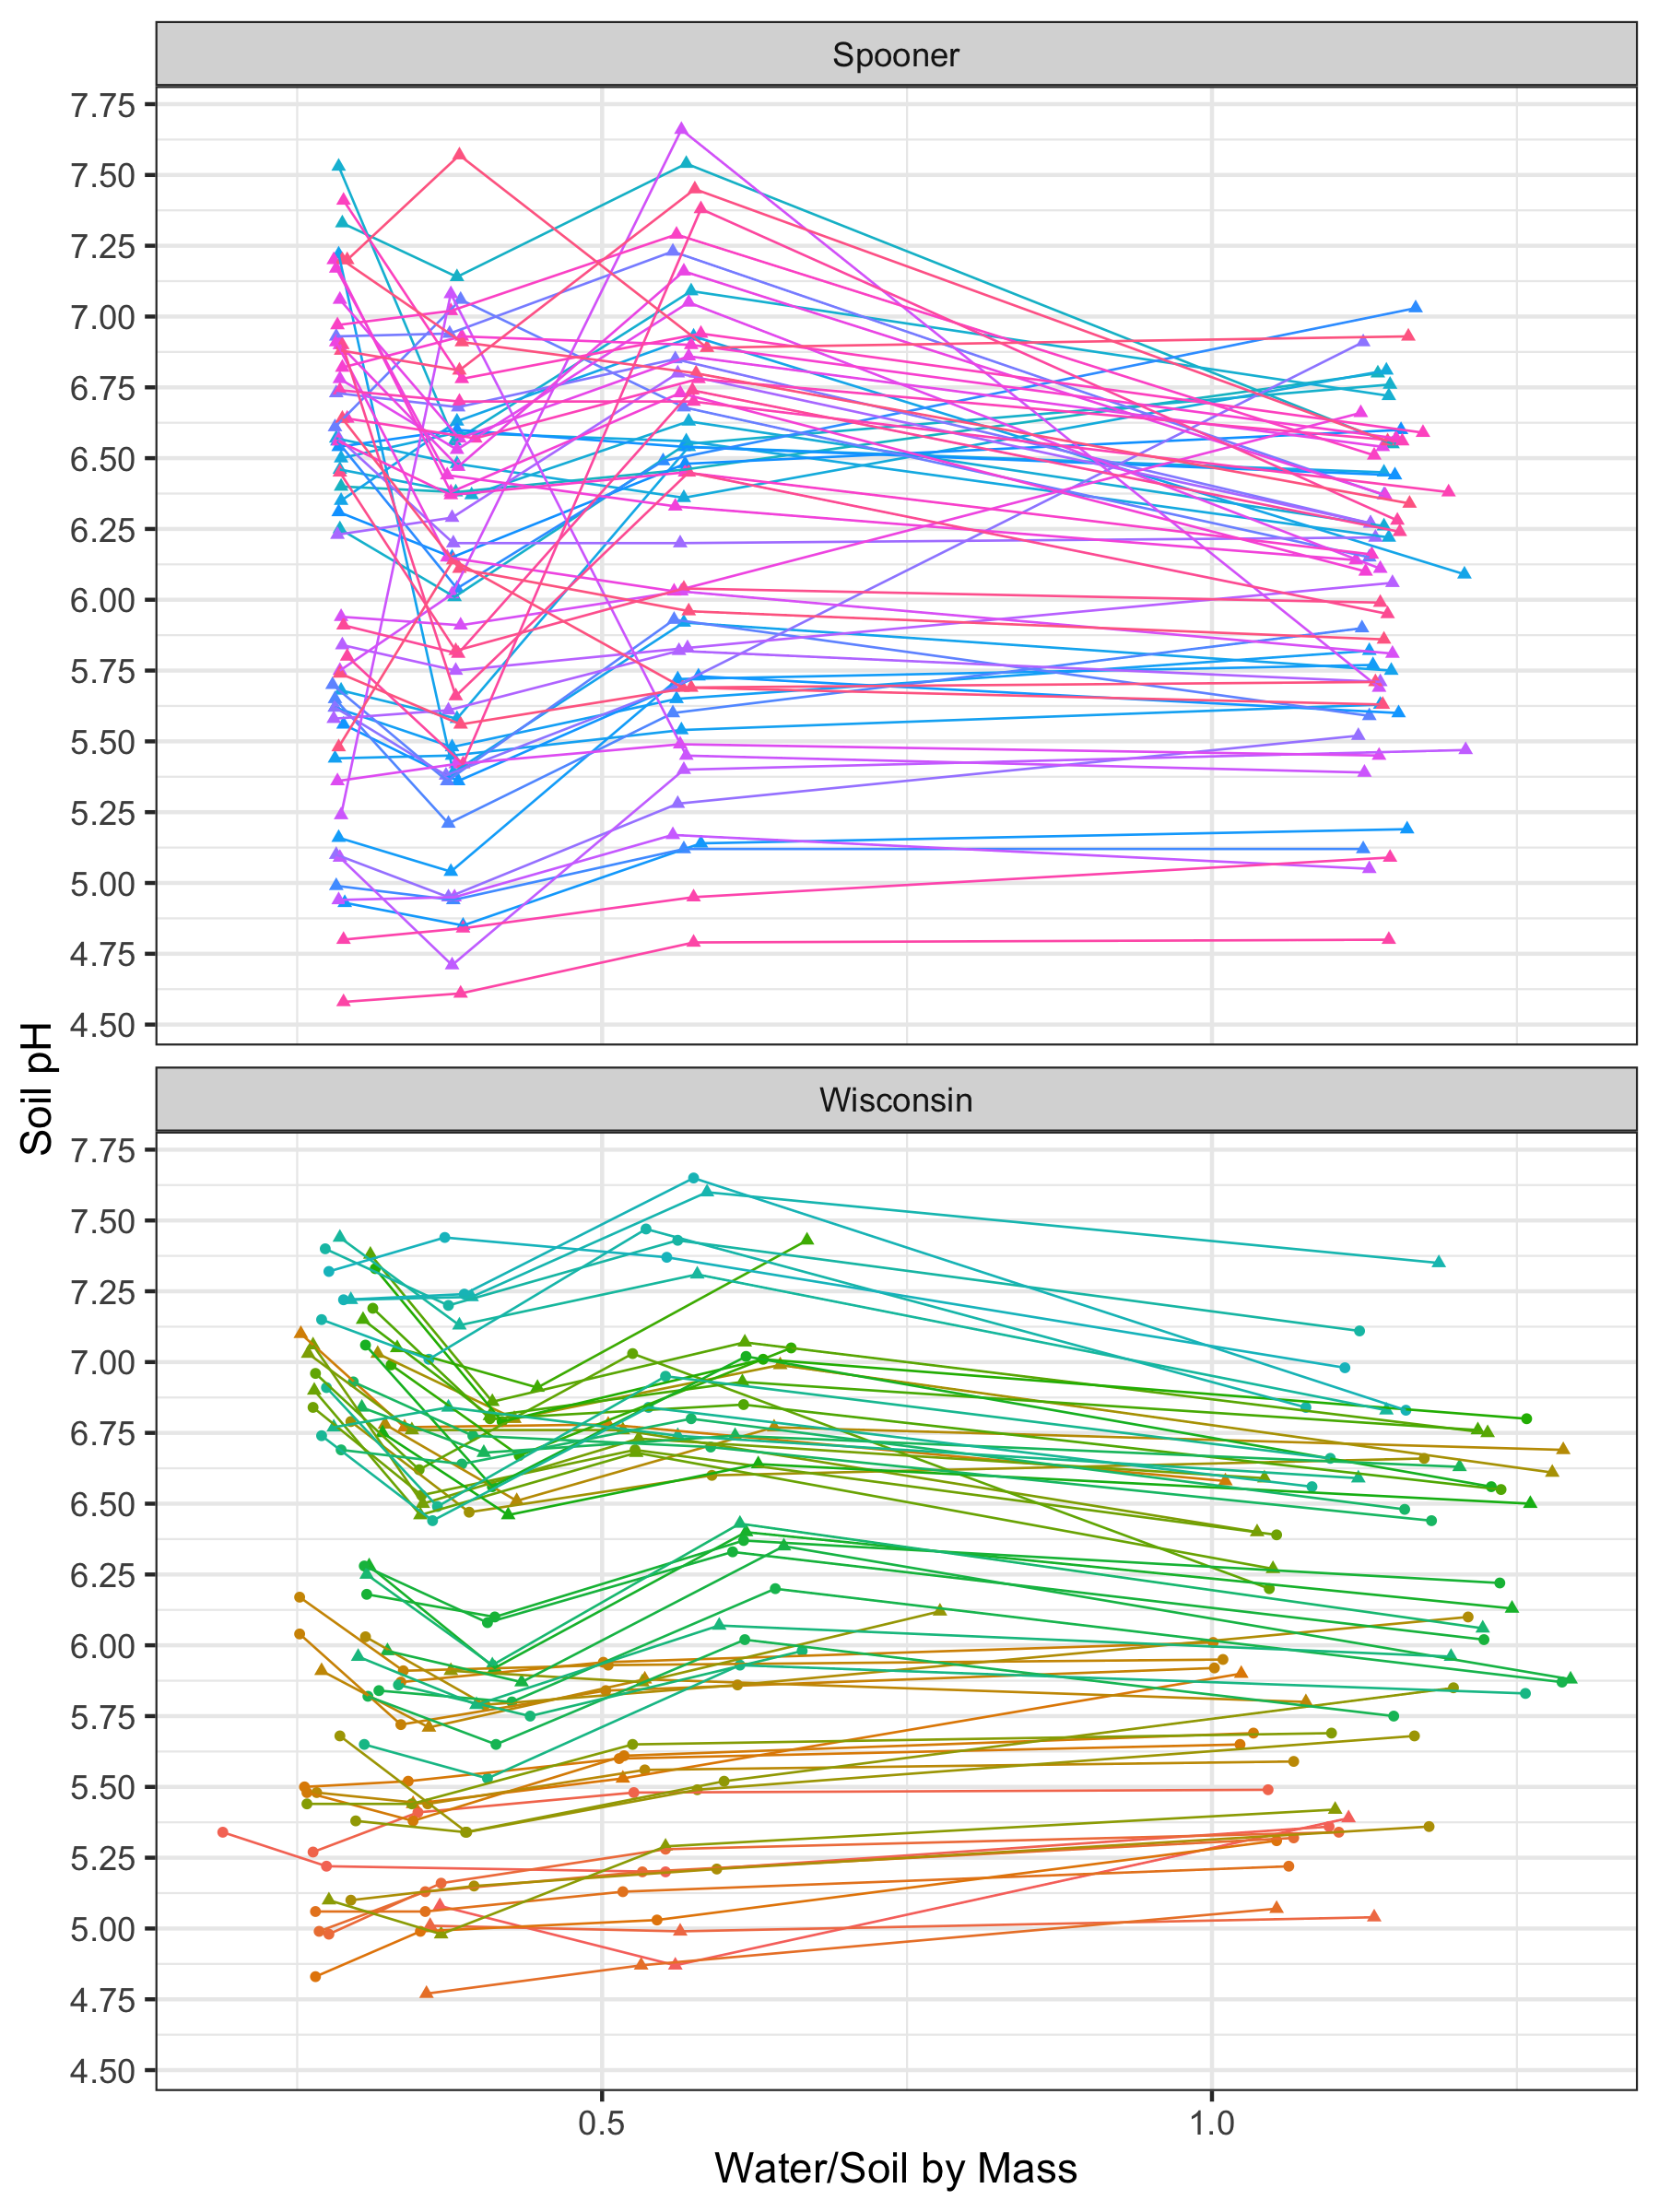
\includegraphics{output-rmd/jackson-plot-ph-1.png}

\begin{Shaded}
\begin{Highlighting}[]
\NormalTok{jack.wisc <-}\StringTok{ }\KeywordTok{ggplot}\NormalTok{(}\KeywordTok{subset}\NormalTok{(dat, Study}\OperatorTok{!=}\StringTok{""}\OperatorTok{&}\NormalTok{Study}\OperatorTok{!=}\StringTok{"Spooner"}\OperatorTok{&}\NormalTok{Real.Water.Soil.ratio}\OperatorTok{<=}\FloatTok{1.3}\NormalTok{), }\KeywordTok{aes}\NormalTok{(Real.Water.Soil.ratio, Lab.CO2.pH, }\DataTypeTok{color=}\NormalTok{Sample.ID, }\DataTypeTok{shape=}\NormalTok{Horizon)) }\OperatorTok{+}\StringTok{ }
\StringTok{  }\KeywordTok{geom_point}\NormalTok{(}\DataTypeTok{size=}\DecValTok{3}\NormalTok{) }\OperatorTok{+}\StringTok{ }\KeywordTok{geom_point}\NormalTok{(}\DataTypeTok{colour =} \StringTok{"grey90"}\NormalTok{, }\DataTypeTok{size =} \FloatTok{1.5}\NormalTok{) }\OperatorTok{+}\StringTok{ }\KeywordTok{geom_line}\NormalTok{(}\DataTypeTok{size=}\FloatTok{0.3}\NormalTok{) }\OperatorTok{+}\StringTok{ }\KeywordTok{theme_bw}\NormalTok{() }\OperatorTok{+}\StringTok{ }\KeywordTok{theme}\NormalTok{(}\DataTypeTok{legend.position=}\StringTok{"none"}\NormalTok{) }\OperatorTok{+}
\StringTok{  }\KeywordTok{facet_wrap}\NormalTok{(}\OperatorTok{~}\NormalTok{Station.Name, }\DataTypeTok{ncol=}\DecValTok{3}\NormalTok{) }\OperatorTok{+}\StringTok{ }\KeywordTok{labs}\NormalTok{(}\DataTypeTok{x=}\StringTok{"Water/Soil by Mass"}\NormalTok{, }\DataTypeTok{y=}\StringTok{"Soil pH"}\NormalTok{) }\OperatorTok{+}\StringTok{ }
\StringTok{  }\KeywordTok{scale_y_continuous}\NormalTok{(}\DataTypeTok{breaks =} \KeywordTok{seq}\NormalTok{(}\DecValTok{4}\NormalTok{, }\DecValTok{8}\NormalTok{, }\DataTypeTok{by =} \FloatTok{0.25}\NormalTok{))}\OperatorTok{+}
\StringTok{  }\KeywordTok{scale_x_continuous}\NormalTok{(}\DataTypeTok{breaks =} \KeywordTok{seq}\NormalTok{(}\DecValTok{0}\NormalTok{, }\FloatTok{1.25}\NormalTok{, }\DataTypeTok{by =} \FloatTok{0.2}\NormalTok{))}
\NormalTok{jack.wisc}
\end{Highlighting}
\end{Shaded}

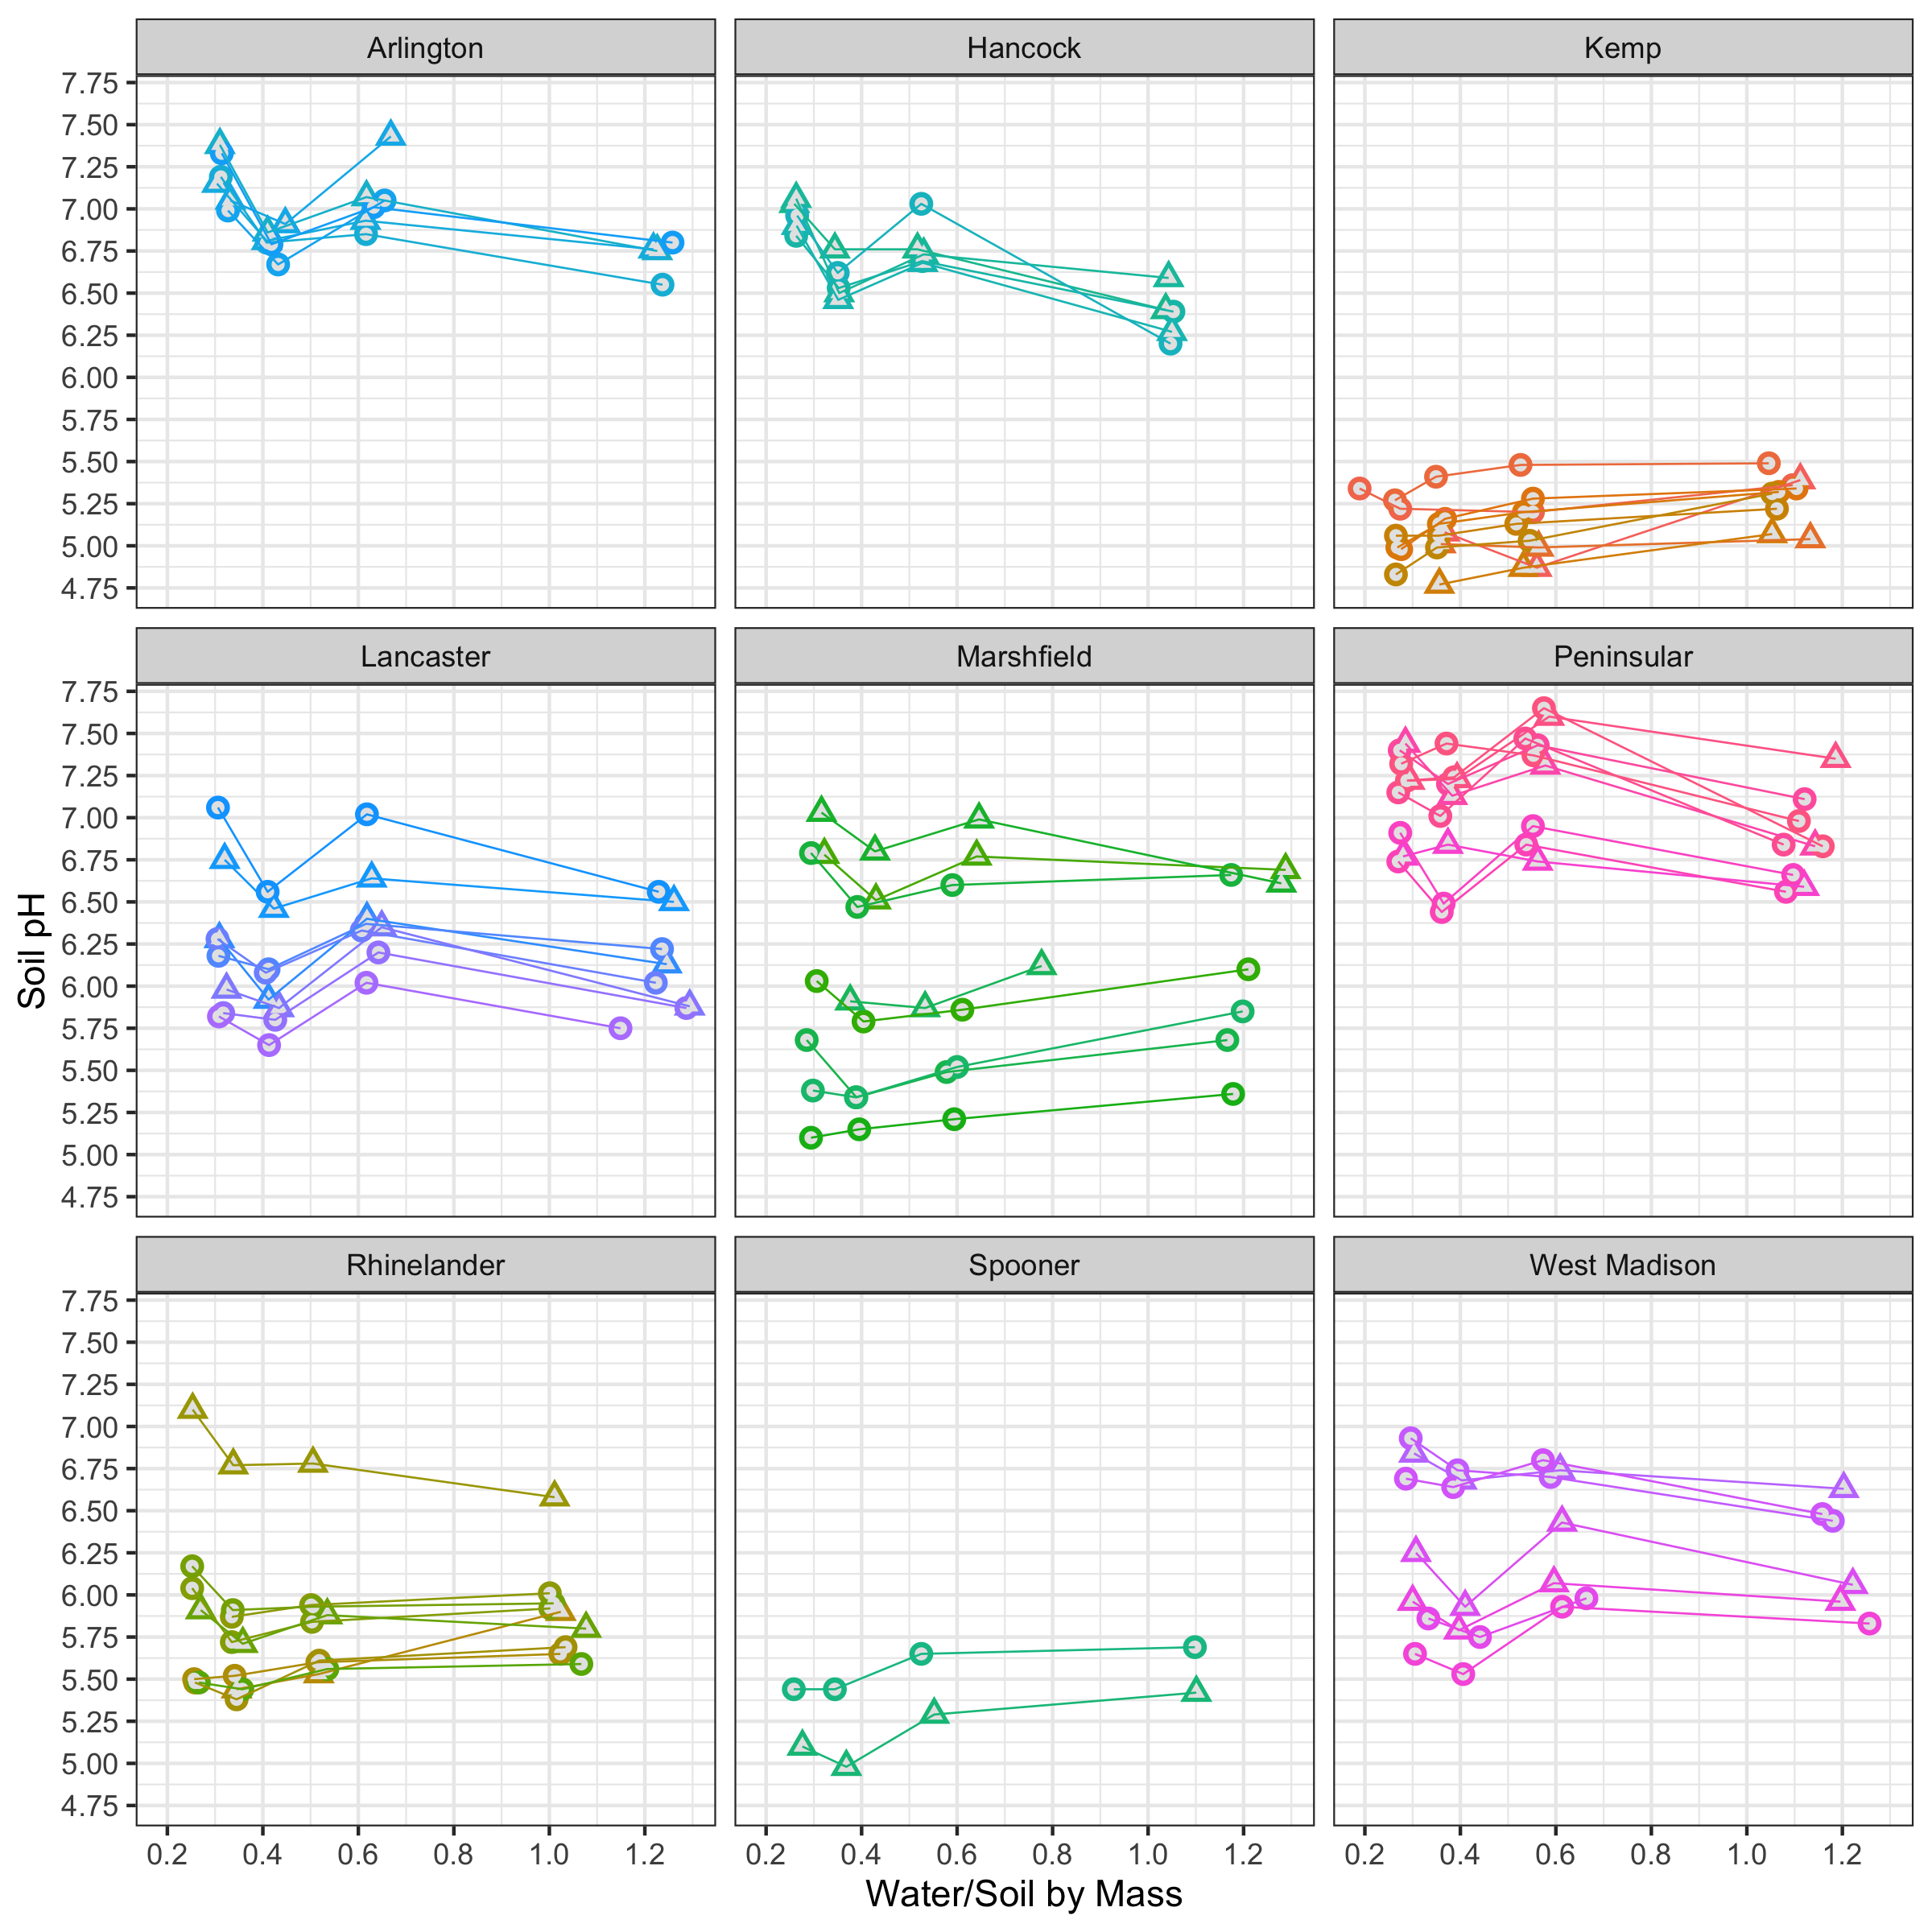
\includegraphics{output-rmd/jackson-plot-ph-wisc-1.png}

\begin{Shaded}
\begin{Highlighting}[]
\NormalTok{jack.spoon <-}\StringTok{ }\KeywordTok{ggplot}\NormalTok{(}\KeywordTok{subset}\NormalTok{(dat, Study}\OperatorTok{!=}\StringTok{""}\OperatorTok{&}\NormalTok{Study}\OperatorTok{!=}\StringTok{"Wisconsin"}\OperatorTok{&}\NormalTok{Real.Water.Soil.ratio}\OperatorTok{<=}\FloatTok{1.3}\NormalTok{), }\KeywordTok{aes}\NormalTok{(Real.Water.Soil.ratio, Lab.CO2.pH, }\DataTypeTok{color=}\NormalTok{Sample.ID, }\DataTypeTok{shape=}\NormalTok{Horizon)) }\OperatorTok{+}\StringTok{ }
\StringTok{  }\KeywordTok{geom_point}\NormalTok{(}\DataTypeTok{size=}\DecValTok{3}\NormalTok{) }\OperatorTok{+}\StringTok{ }\KeywordTok{geom_point}\NormalTok{(}\DataTypeTok{colour =} \StringTok{"grey90"}\NormalTok{, }\DataTypeTok{size =} \FloatTok{1.5}\NormalTok{) }\OperatorTok{+}\StringTok{ }\KeywordTok{geom_line}\NormalTok{(}\DataTypeTok{size=}\FloatTok{0.3}\NormalTok{) }\OperatorTok{+}\StringTok{ }\KeywordTok{theme_bw}\NormalTok{() }\OperatorTok{+}\StringTok{ }\KeywordTok{theme}\NormalTok{(}\DataTypeTok{legend.position=}\StringTok{"none"}\NormalTok{) }\OperatorTok{+}
\StringTok{  }\KeywordTok{facet_wrap}\NormalTok{(}\OperatorTok{~}\NormalTok{Station.Name, }\DataTypeTok{ncol=}\DecValTok{3}\NormalTok{) }\OperatorTok{+}\StringTok{ }\KeywordTok{labs}\NormalTok{(}\DataTypeTok{x=}\StringTok{"Water/Soil by Mass"}\NormalTok{, }\DataTypeTok{y=}\StringTok{"Soil pH"}\NormalTok{) }\OperatorTok{+}\StringTok{ }
\StringTok{  }\KeywordTok{scale_y_continuous}\NormalTok{(}\DataTypeTok{breaks =} \KeywordTok{seq}\NormalTok{(}\DecValTok{4}\NormalTok{, }\DecValTok{8}\NormalTok{, }\DataTypeTok{by =} \FloatTok{0.25}\NormalTok{))}\OperatorTok{+}
\StringTok{  }\KeywordTok{scale_x_continuous}\NormalTok{(}\DataTypeTok{breaks =} \KeywordTok{seq}\NormalTok{(}\DecValTok{0}\NormalTok{, }\FloatTok{1.25}\NormalTok{, }\DataTypeTok{by =} \FloatTok{0.2}\NormalTok{))}
\NormalTok{jack.spoon}
\end{Highlighting}
\end{Shaded}

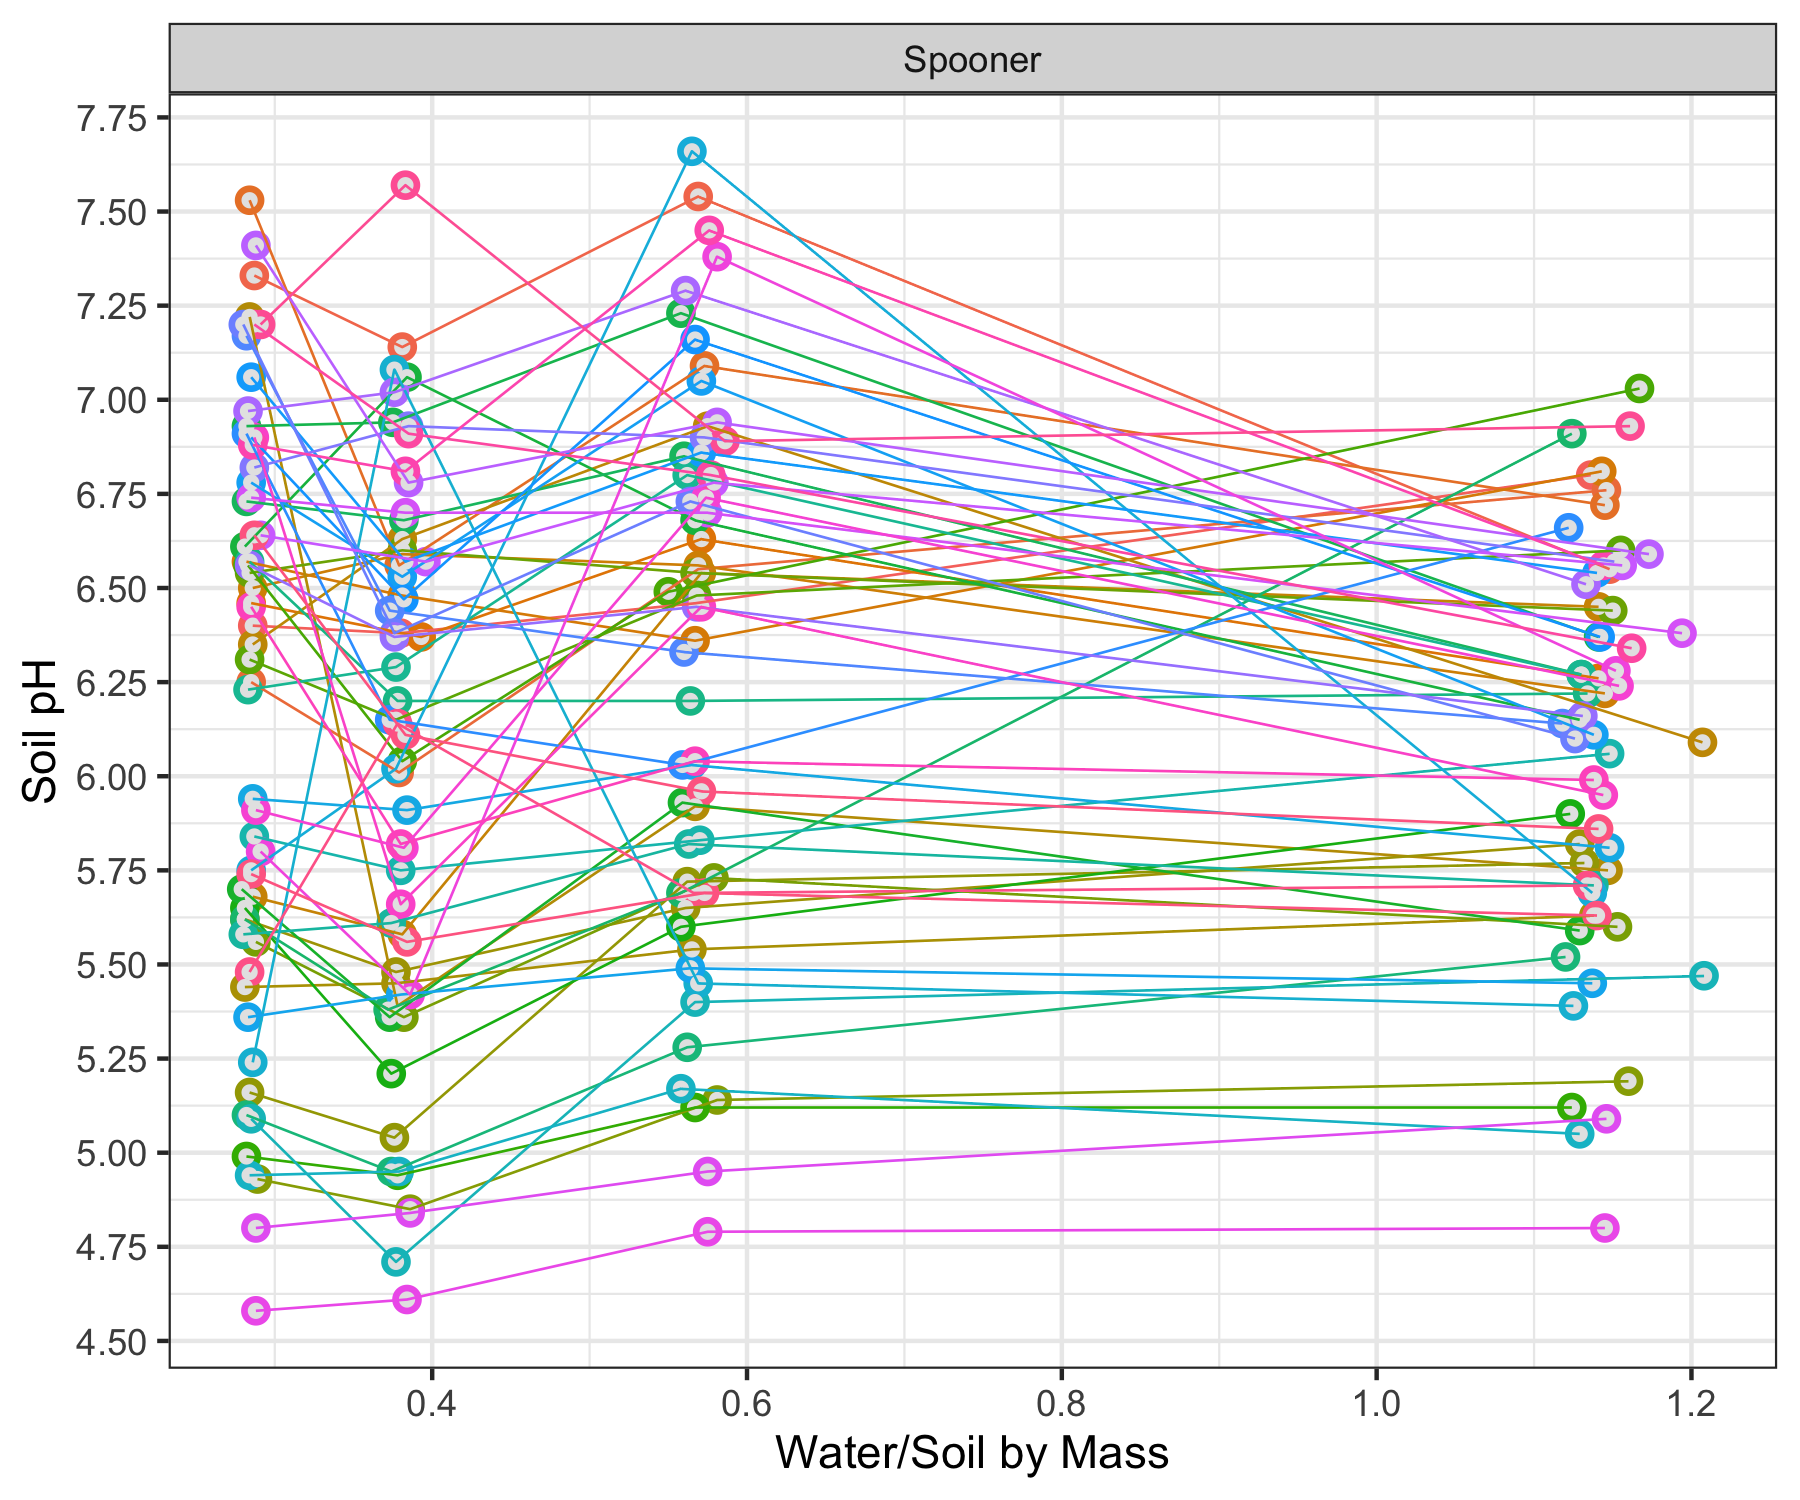
\includegraphics{output-rmd/jackson-plot-ph-spooner-1.png}

\begin{Shaded}
\begin{Highlighting}[]
\KeywordTok{ggplot}\NormalTok{(}\KeywordTok{subset}\NormalTok{(dat, Study}\OperatorTok{!=}\StringTok{""}\OperatorTok{&}\NormalTok{Study}\OperatorTok{!=}\StringTok{"Spooner"}\OperatorTok{&}\NormalTok{Real.Water.Soil.ratio}\OperatorTok{<=}\FloatTok{1.3}\NormalTok{), }\KeywordTok{aes}\NormalTok{(Real.Water.Soil.ratio, }\DecValTok{10}\OperatorTok{^-}\NormalTok{Lab.CO2.pH, }\DataTypeTok{color=}\NormalTok{Sample.ID, }\DataTypeTok{shape=}\NormalTok{Horizon)) }\OperatorTok{+}\StringTok{ }
\StringTok{  }\KeywordTok{geom_point}\NormalTok{(}\DataTypeTok{size=}\DecValTok{2}\NormalTok{) }\OperatorTok{+}\StringTok{ }\KeywordTok{geom_line}\NormalTok{(}\DataTypeTok{size=}\FloatTok{0.3}\NormalTok{) }\OperatorTok{+}\StringTok{ }\KeywordTok{theme_bw}\NormalTok{() }\OperatorTok{+}\StringTok{ }\KeywordTok{theme}\NormalTok{(}\DataTypeTok{legend.position=}\StringTok{"none"}\NormalTok{) }\OperatorTok{+}
\StringTok{  }\KeywordTok{facet_wrap}\NormalTok{(}\OperatorTok{~}\NormalTok{Station.Name, }\DataTypeTok{ncol=}\DecValTok{3}\NormalTok{) }\OperatorTok{+}\StringTok{ }\KeywordTok{labs}\NormalTok{(}\DataTypeTok{x=}\StringTok{"Water/Soil by Mass"}\NormalTok{, }\DataTypeTok{y=}\StringTok{"Soil a(H+)"}\NormalTok{)}
\end{Highlighting}
\end{Shaded}

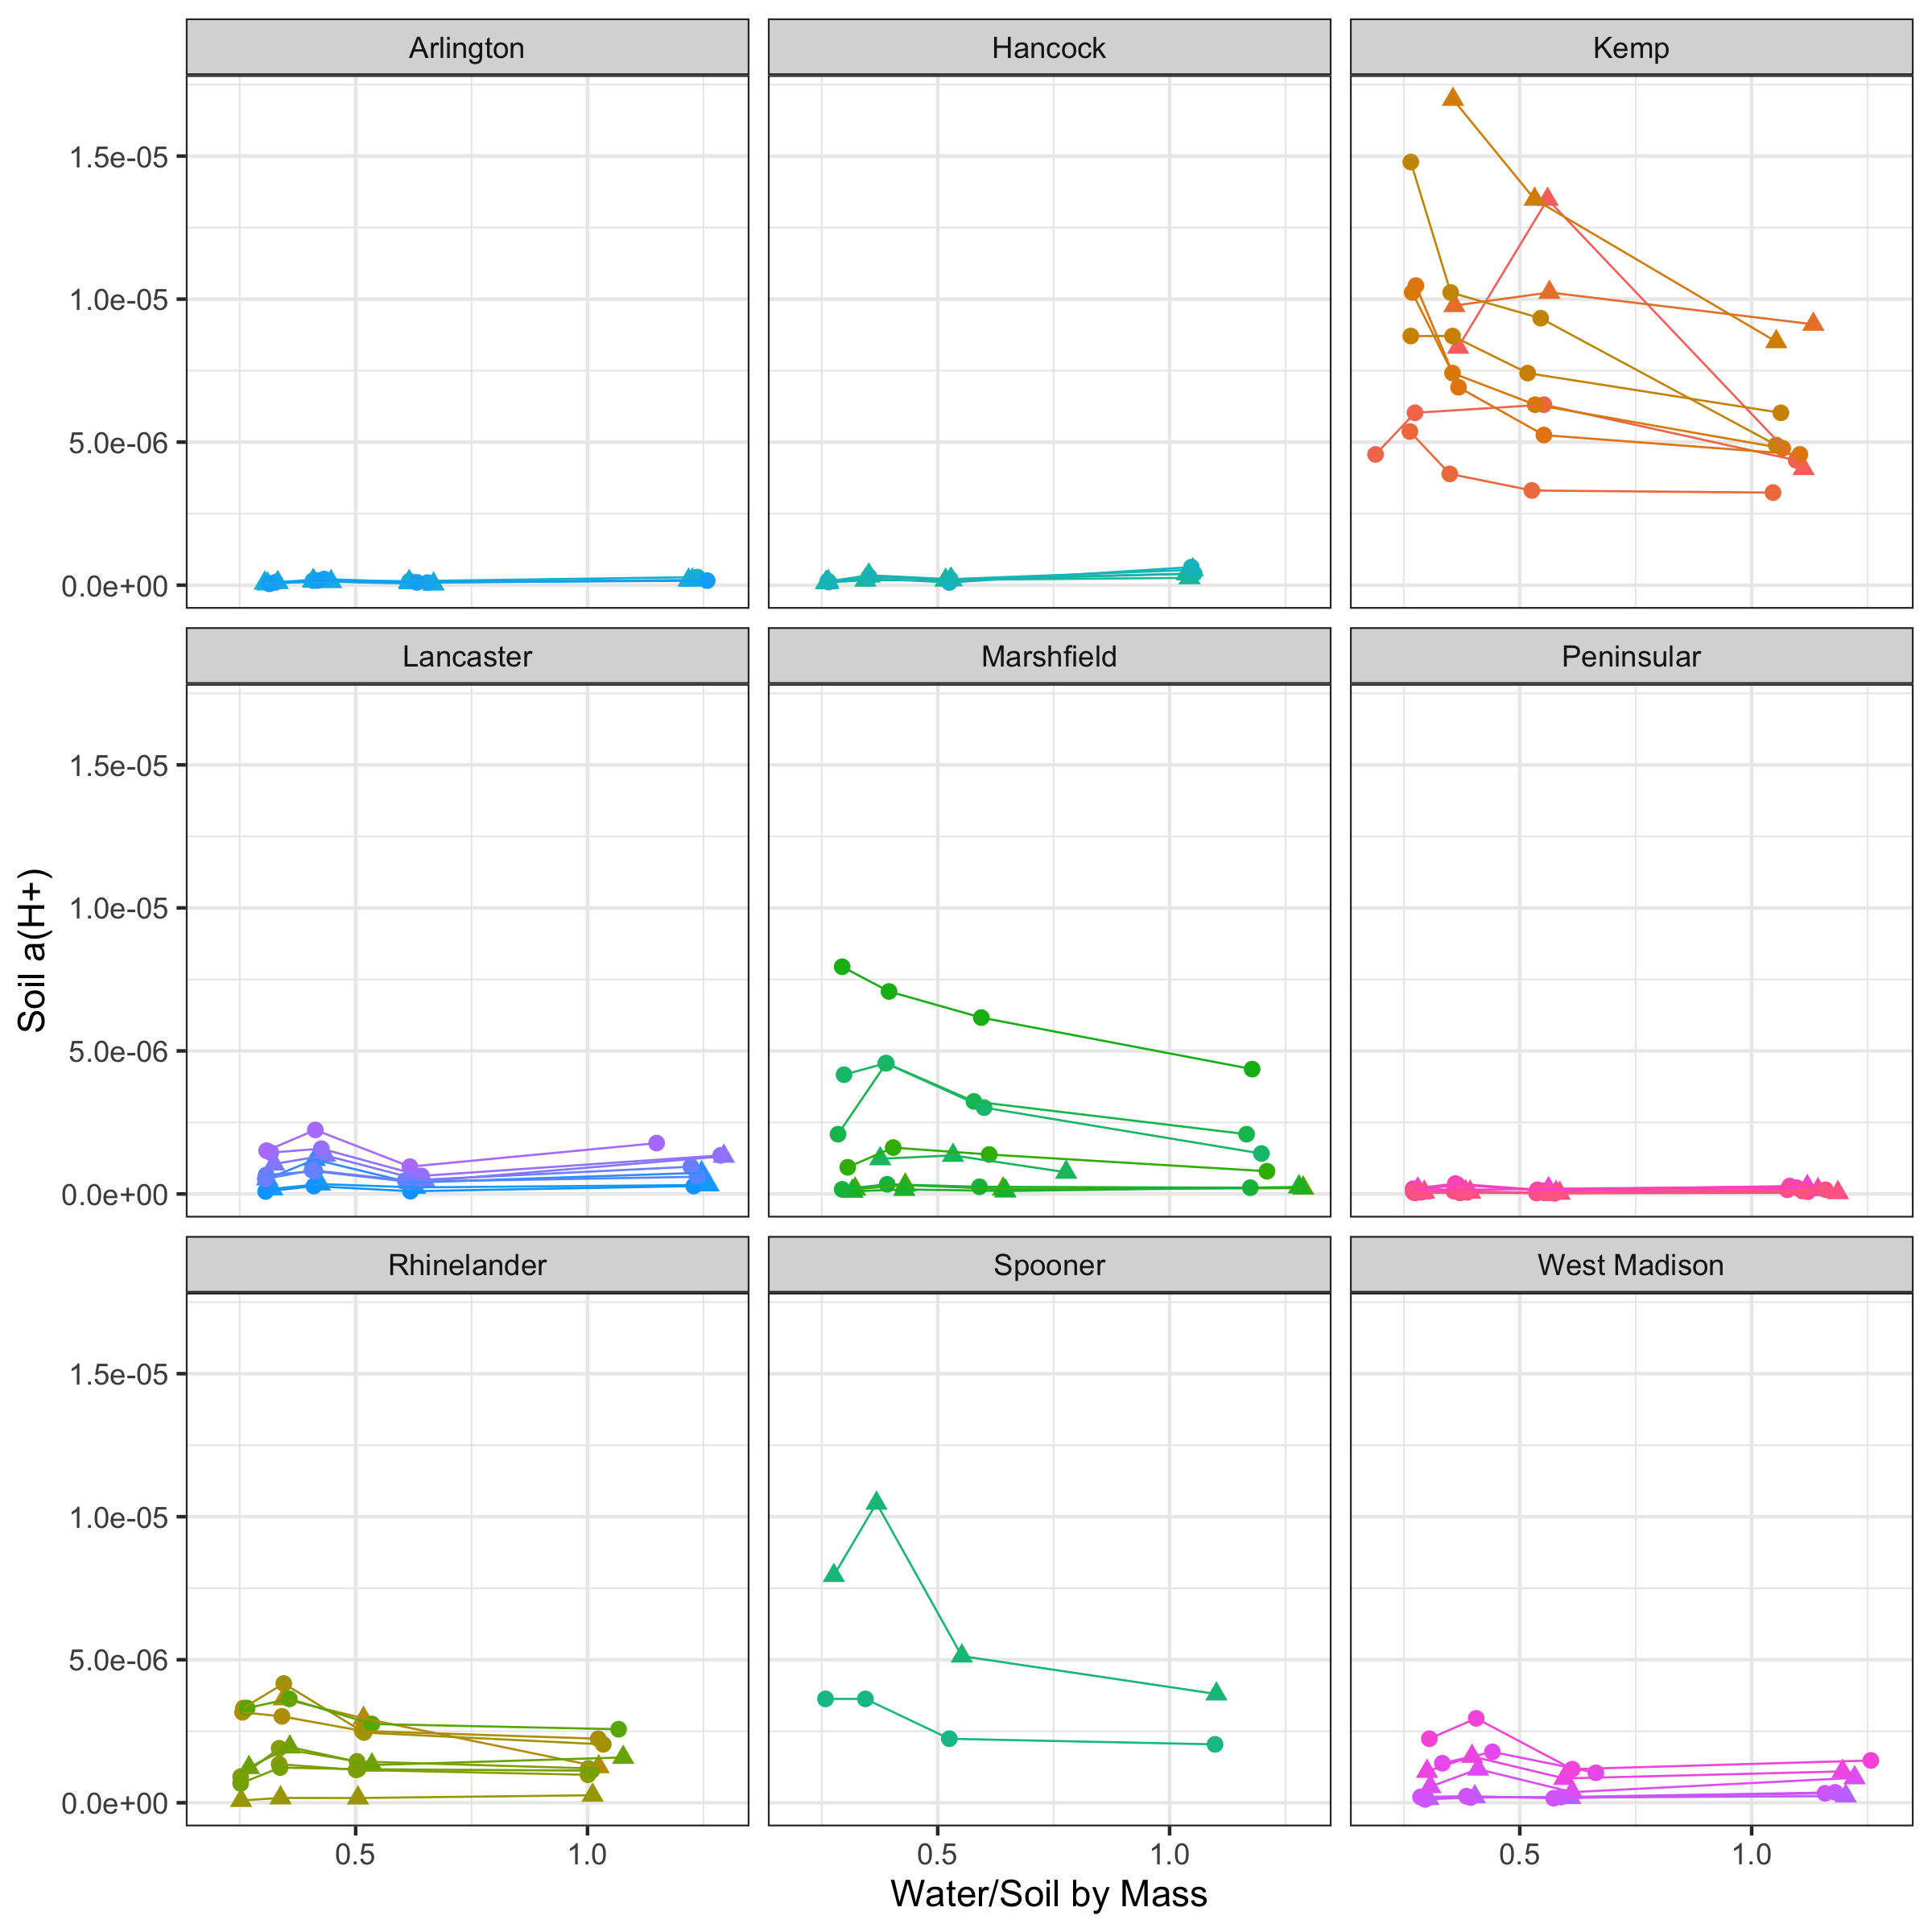
\includegraphics{output-rmd/jackson-plot-activity-wisc-1.png}

\begin{Shaded}
\begin{Highlighting}[]
\KeywordTok{ggplot}\NormalTok{(}\KeywordTok{subset}\NormalTok{(dat, Study}\OperatorTok{!=}\StringTok{""}\OperatorTok{&}\NormalTok{Study}\OperatorTok{!=}\StringTok{"Wisconsin"}\OperatorTok{&}\NormalTok{Real.Water.Soil.ratio}\OperatorTok{<=}\FloatTok{1.3}\NormalTok{), }\KeywordTok{aes}\NormalTok{(Real.Water.Soil.ratio, }\DecValTok{10}\OperatorTok{^-}\NormalTok{Lab.CO2.pH, }\DataTypeTok{color=}\NormalTok{Sample.ID, }\DataTypeTok{shape=}\NormalTok{Horizon)) }\OperatorTok{+}\StringTok{ }
\StringTok{  }\KeywordTok{geom_point}\NormalTok{(}\DataTypeTok{size=}\DecValTok{2}\NormalTok{) }\OperatorTok{+}\StringTok{ }\KeywordTok{geom_line}\NormalTok{(}\DataTypeTok{size=}\FloatTok{0.3}\NormalTok{) }\OperatorTok{+}\StringTok{ }\KeywordTok{theme_bw}\NormalTok{() }\OperatorTok{+}\StringTok{ }\KeywordTok{theme}\NormalTok{(}\DataTypeTok{legend.position=}\StringTok{"none"}\NormalTok{) }\OperatorTok{+}
\StringTok{  }\KeywordTok{facet_wrap}\NormalTok{(}\OperatorTok{~}\NormalTok{Station.Name, }\DataTypeTok{ncol=}\DecValTok{3}\NormalTok{) }\OperatorTok{+}\StringTok{ }\KeywordTok{labs}\NormalTok{(}\DataTypeTok{x=}\StringTok{"Water/Soil by Mass"}\NormalTok{, }\DataTypeTok{y=}\StringTok{"Soil a(H+)"}\NormalTok{)}
\end{Highlighting}
\end{Shaded}

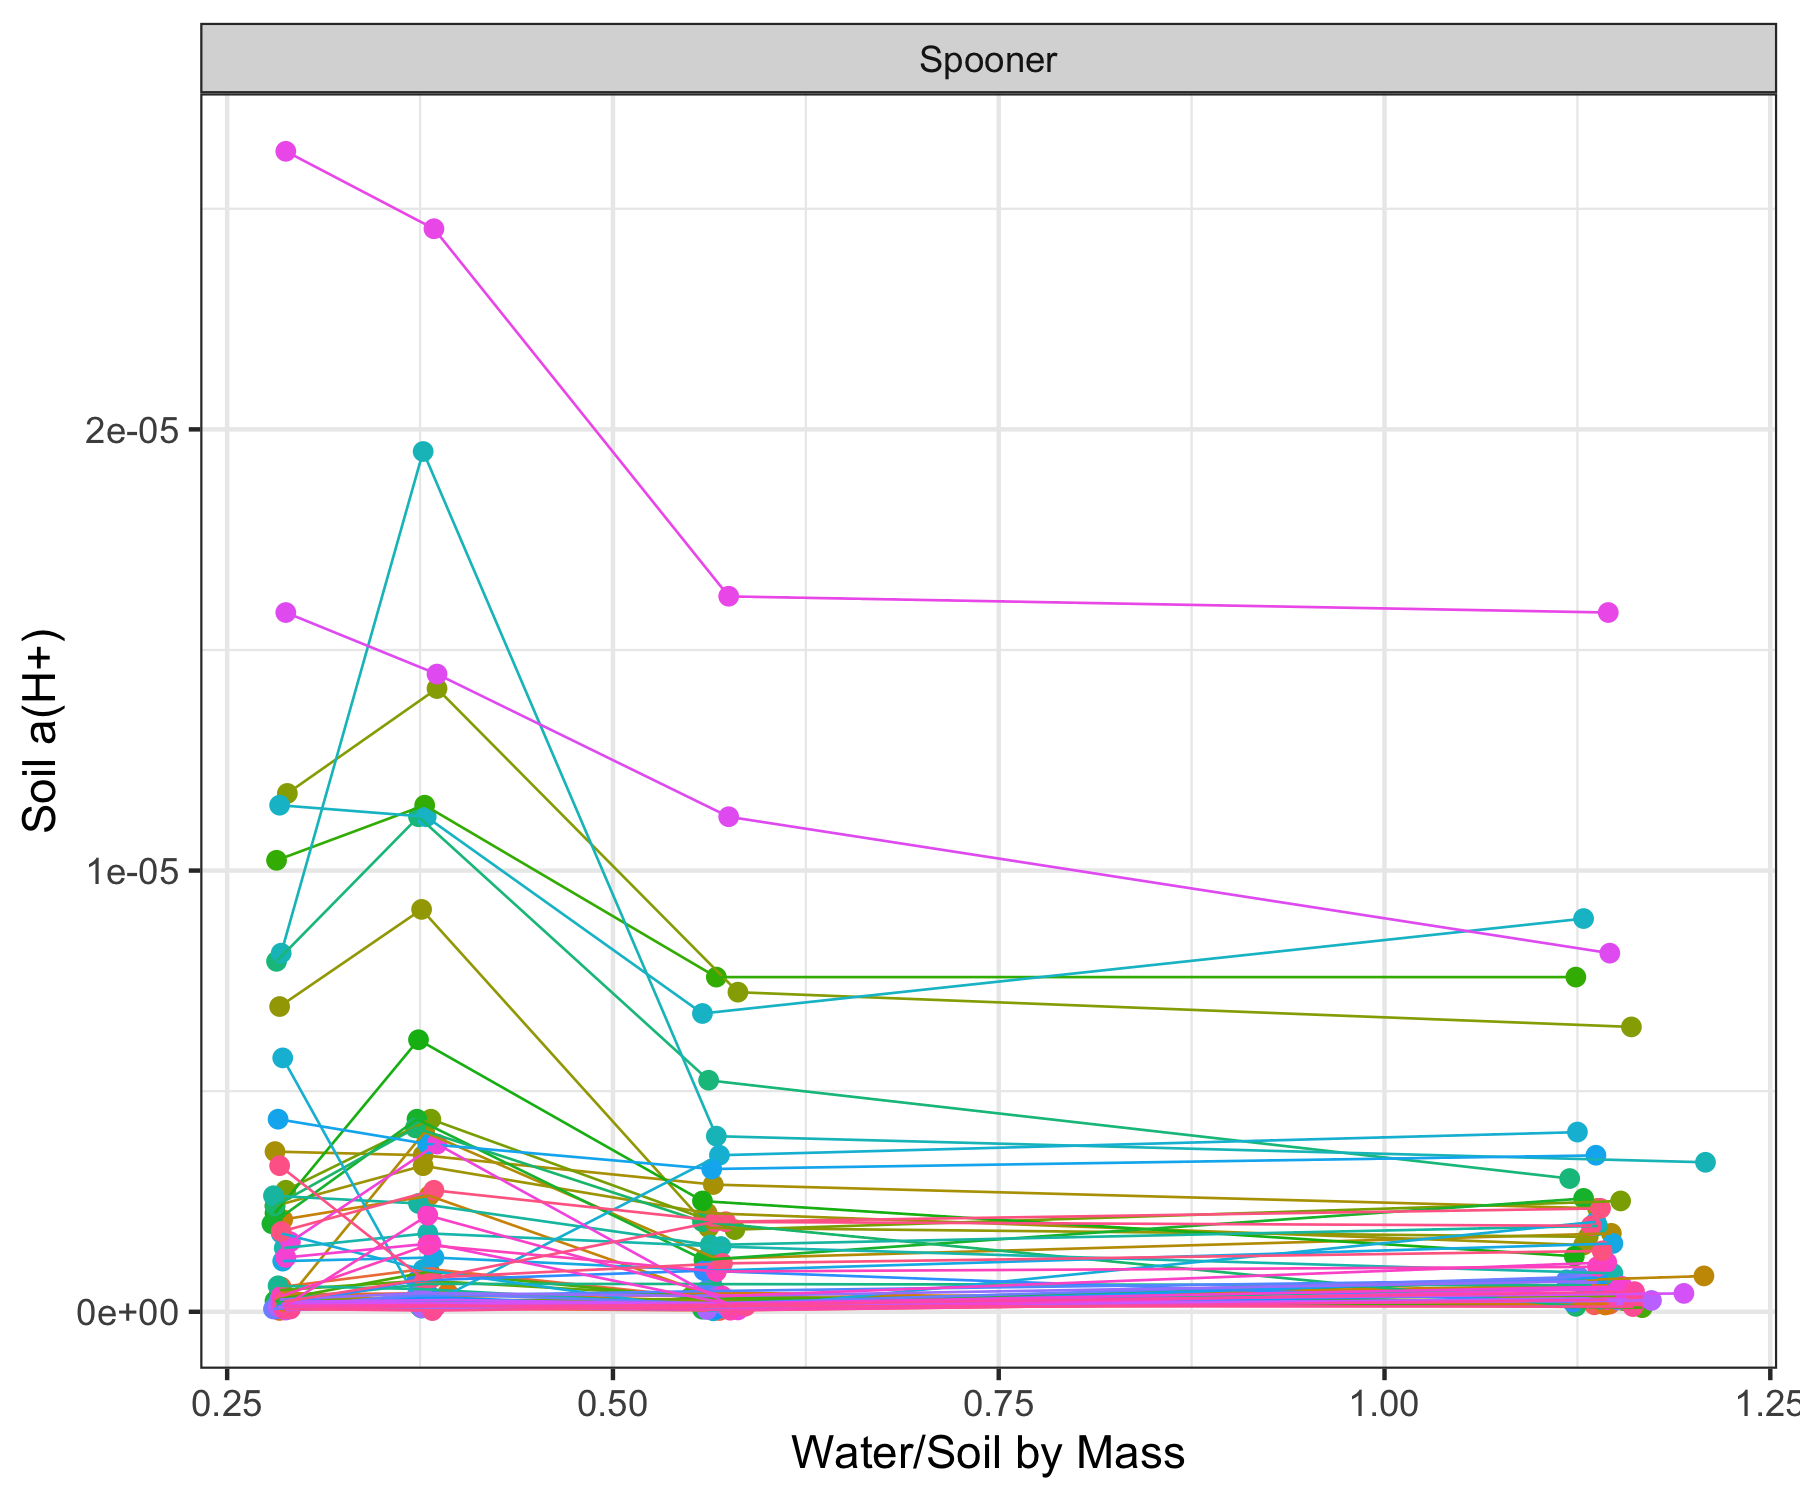
\includegraphics{output-rmd/jackson-plot-activity-spooner-1.png}

\begin{Shaded}
\begin{Highlighting}[]
\KeywordTok{plot_grid}\NormalTok{(jack.spoon, jack.wisc)}
\end{Highlighting}
\end{Shaded}

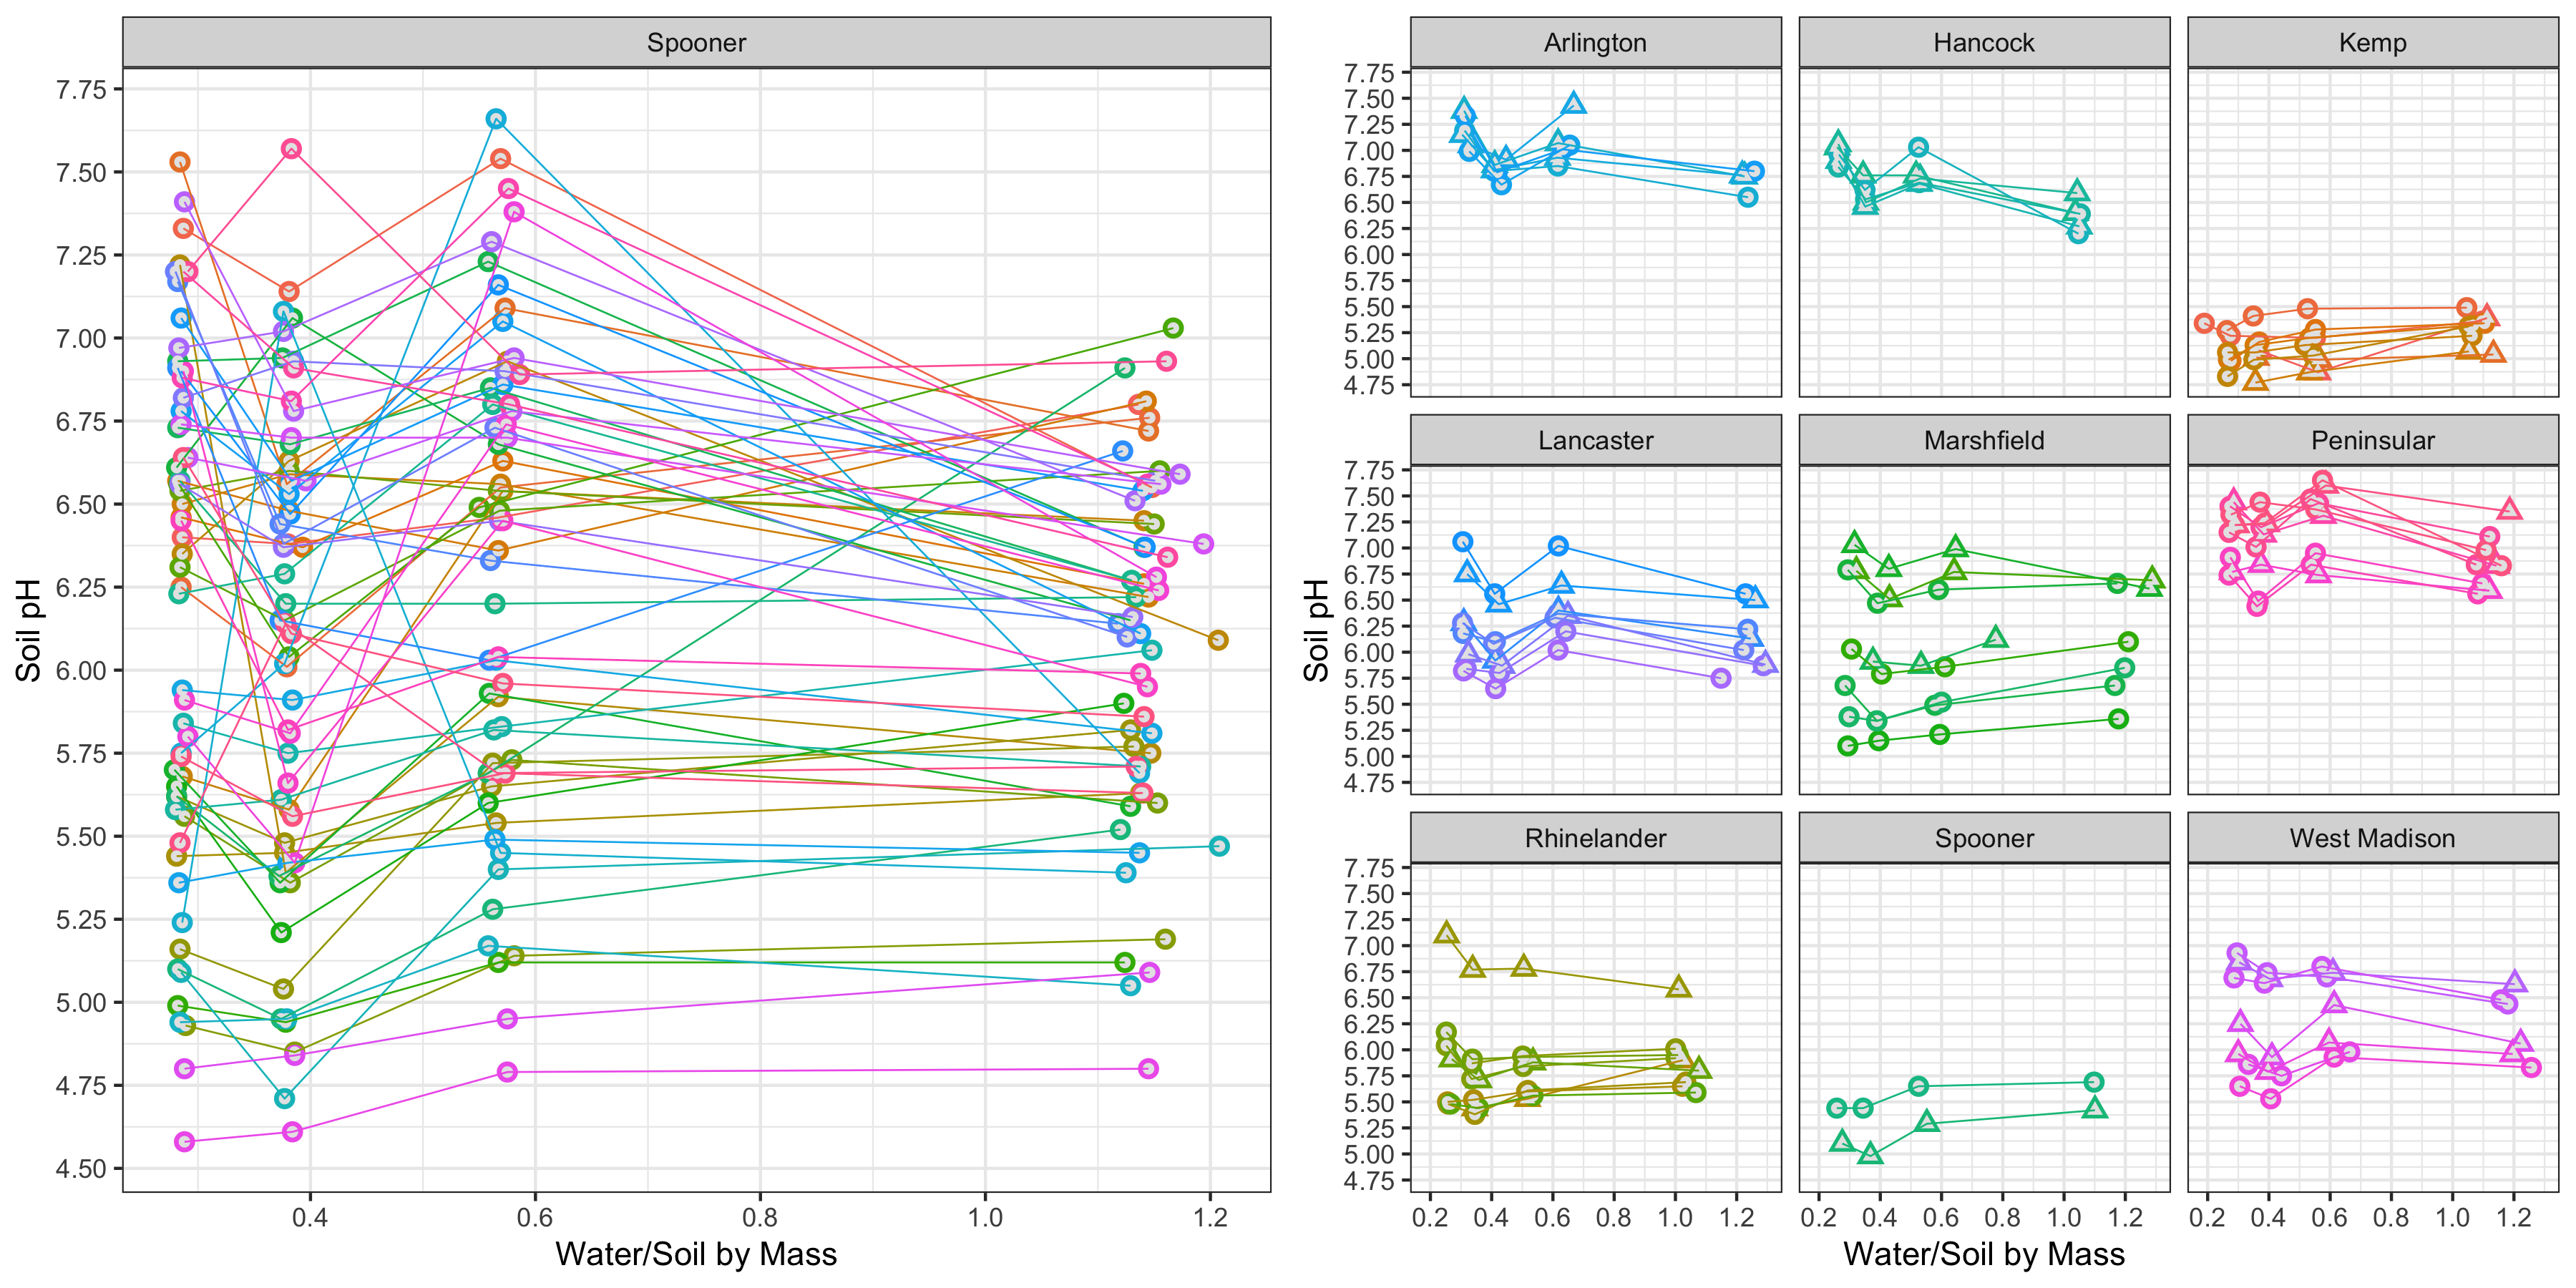
\includegraphics{output-rmd/jackson-plot-wiscons-spooner-1.png}

\hypertarget{wisconsin-soil-ph-nutrient-profiles}{%
\subsection{Wisconsin Soil pH \textasciitilde{} Nutrient
Profiles}\label{wisconsin-soil-ph-nutrient-profiles}}

This is the BIC for the Wisconsin soils, using the available
``metadata'', which means soil chemical data.

\begin{Shaded}
\begin{Highlighting}[]
\NormalTok{dat.wisc <-}\StringTok{ }\KeywordTok{subset}\NormalTok{(dat, Study}\OperatorTok{==}\StringTok{"Wisconsin"}\NormalTok{)}
\end{Highlighting}
\end{Shaded}

\hypertarget{one2one}{%
\subsubsection{one2one}\label{one2one}}

\begin{Shaded}
\begin{Highlighting}[]
\NormalTok{dat.wisc.}\FloatTok{1.}\NormalTok{to}\FloatTok{.1}\NormalTok{ <-}\StringTok{ }\KeywordTok{subset}\NormalTok{(dat.wisc, Water.Soil.Ratio}\OperatorTok{==}\StringTok{"1-to-1"}\NormalTok{)}
\KeywordTok{str}\NormalTok{(dat.wisc.}\FloatTok{1.}\NormalTok{to}\FloatTok{.1}\NormalTok{)}
\end{Highlighting}
\end{Shaded}

\begin{verbatim}
## 'data.frame':    63 obs. of  47 variables:
##  $ Horizon                  : chr  "Topsoil" "Subsoil" "Subsoil" "Topsoil" ...
##  $ Water.Soil.Ratio         : chr  "1-to-1" "1-to-1" "1-to-1" "1-to-1" ...
##  $ Sample.ID                : chr  "001-K1-0-17" "002-K1-17-45" "003-K1-45-60" "005-K3-0-15" ...
##  $ Study                    : chr  "Wisconsin" "Wisconsin" "Wisconsin" "Wisconsin" ...
##  $ Sample.Number            : int  1 2 3 5 6 7 8 9 10 11 ...
##  $ DNA.Extr.pH.After.C1     : num  8.83 9.12 9.38 8.69 9.03 ...
##  $ DNA.Extr.pH.After.C2     : num  7.78 8 7.98 7.72 7.9 ...
##  $ Lab.CO2.pH               : num  5.39 5.36 5.49 5.04 5.34 5.32 5.07 5.22 5.31 5.9 ...
##  $ High.CO2.pH              : num  5.13 5.1 5.33 4.87 5.2 5.15 4.74 5.15 4.98 5.79 ...
##  $ Tube.Empty.g             : num  1.06 1.07 1.06 1.07 1.05 ...
##  $ Moist.Soil.g             : num  0.756 0.785 0.813 0.807 0.826 0.76 0.795 0.859 0.828 0.796 ...
##  $ Water.Added.mL           : num  0.756 0.785 0.813 0.807 0.826 0.76 0.795 0.859 0.828 0.796 ...
##  $ Tube.Dry.Soil.g          : num  1.74 1.78 1.84 1.78 1.8 ...
##  $ Dry.Soil.g               : num  0.68 0.716 0.777 0.712 0.748 0.712 0.755 0.808 0.786 0.777 ...
##  $ Water.Cont.mass          : num  0.101 0.088 0.044 0.118 0.094 0.063 0.05 0.059 0.051 0.024 ...
##  $ Target.Water.Soil.Content: num  1 1 1 1 1 1 1 1 1 1 ...
##  $ Real.Water.Soil.ratio    : num  1.11 1.1 1.05 1.13 1.1 ...
##  $ Error.Water.Soil.ratio   : num  -0.112 -0.096 -0.046 -0.133 -0.104 -0.067 -0.053 -0.063 -0.053 -0.024 ...
##  $ Perc.Sand                : num  64 68 72 64 60 70 78 74 72 82 ...
##  $ Perc.Silt                : num  25.2 21.2 19.2 27.2 31.2 19.2 15.2 15.2 15.2 11.2 ...
##  $ Perc.Clay                : num  10.8 10.8 8.8 8.8 8.8 10.8 6.8 10.8 12.8 6.8 ...
##  $ Texture.Name             : chr  "Sandy Loam" "Sandy Loam" "Sandy Loam" "Sandy Loam" ...
##  $ OM.perc                  : num  2.5 1.3 0.4 4 1.5 0.8 2.5 1.4 0.8 1.2 ...
##  $ Scoop.Density.g.4.24.cc  : num  4.6 5.36 6.28 4.38 5.05 5.76 4.89 5.44 5.51 6.16 ...
##  $ Soil.pH                  : num  4.9 5.4 5.6 4.7 5.1 5.2 4.5 5 4.4 5.5 ...
##  $ Sikora.pH                : num  6.3 6.5 7.1 6.1 6.4 6.7 6.1 6.4 6.5 6.8 ...
##  $ Total.N.perc             : num  0.13 0.09 0.08 0.18 0.12 0.11 0.13 0.11 0.11 0.13 ...
##  $ Total.Org.C.perc         : num  1.64 0.71 0.11 2.52 0.77 0.33 1.63 0.68 0.34 0.81 ...
##  $ Bray.1.P.ppm             : int  99 101 37 63 40 24 18 64 16 197 ...
##  $ K.ppm                    : int  44 41 26 67 57 63 42 29 23 62 ...
##  $ K.perc.CEC               : int  1 1 4 1 2 3 1 1 1 6 ...
##  $ Ca.ppm                   : int  237 194 327 382 170 189 122 22 22 134 ...
##  $ Ca.perc.CEC              : int  12 13 96 15 11 19 5 1 2 23 ...
##  $ Mg.ppm                   : int  40 32 58 85 39 38 22 6 5 8 ...
##  $ Mg.perc.CEC              : int  3 4 28 5 4 6 2 1 1 2 ...
##  $ Na.ppm                   : logi  NA NA NA NA NA NA ...
##  $ Na.perc.CEC              : int  0 0 0 0 0 0 0 0 0 0 ...
##  $ Est.Ac.Hplus             : num  8.6 6.1 0 10.9 7 4 10.7 7.3 5.5 2 ...
##  $ Hplus.perc.CEC           : int  87 85 0 84 87 78 94 98 97 71 ...
##  $ CEC.sum                  : int  9 6 1 13 7 4 10 6 4 2 ...
##  $ Date.of.Collection       : chr  "8/23/2018" "8/23/2018" "8/23/2018" "8/23/2018" ...
##  $ Station.Name             : chr  "Kemp" "Kemp" "Kemp" "Kemp" ...
##  $ St.pH.WSS                : num  5.4 5.4 5.4 5.4 5.4 5.4 5.4 5.4 5.4 5.5 ...
##  $ Site.Number              : int  1 1 1 3 3 3 4 4 4 1 ...
##  $ Upper.Depth.cm           : int  0 17 45 0 15 35 0 15 30 0 ...
##  $ Lower.Depth.cm           : int  17 45 60 15 35 50 15 30 50 27 ...
##  $ Mean.Depth               : num  8.5 31 52.5 7.5 25 42.5 7.5 22.5 40 13.5 ...
\end{verbatim}

\begin{Shaded}
\begin{Highlighting}[]
\NormalTok{bic.wisc.one2one.labco2 <-}\StringTok{ }\KeywordTok{regsubsets}\NormalTok{(Lab.CO2.pH }\OperatorTok{~}\StringTok{ }\NormalTok{Perc.Sand }\OperatorTok{+}\StringTok{ }\NormalTok{Perc.Silt }\OperatorTok{+}\StringTok{ }\NormalTok{Perc.Clay }\OperatorTok{+}\StringTok{ }\NormalTok{OM.perc }\OperatorTok{+}\StringTok{ }\NormalTok{Total.N.perc }\OperatorTok{+}\StringTok{ }\NormalTok{Total.Org.C.perc }\OperatorTok{+}\StringTok{ }\NormalTok{Bray.}\FloatTok{1.}\NormalTok{P.ppm }\OperatorTok{+}\StringTok{ }\NormalTok{K.ppm }\OperatorTok{+}\StringTok{ }\NormalTok{Ca.ppm }\OperatorTok{+}\StringTok{ }\NormalTok{Mg.ppm }\OperatorTok{+}\StringTok{ }\NormalTok{Est.Ac.Hplus }\OperatorTok{+}\StringTok{ }\NormalTok{CEC.sum }\OperatorTok{+}\StringTok{ }\NormalTok{Mean.Depth, }\DataTypeTok{nbest =} \DecValTok{2}\NormalTok{, }\DataTypeTok{data =}\NormalTok{ dat.wisc.}\FloatTok{1.}\NormalTok{to}\FloatTok{.1}\NormalTok{)}
\end{Highlighting}
\end{Shaded}

\begin{verbatim}
## Reordering variables and trying again:
\end{verbatim}

\begin{Shaded}
\begin{Highlighting}[]
\KeywordTok{plot}\NormalTok{(bic.wisc.one2one.labco2, }\DataTypeTok{scale=}\StringTok{'bic'}\NormalTok{, }\DataTypeTok{main=}\StringTok{"Wisconsin Soils, 1-to-1 Water-to-Soil, ~400 ppm CO2"}\NormalTok{)}
\end{Highlighting}
\end{Shaded}

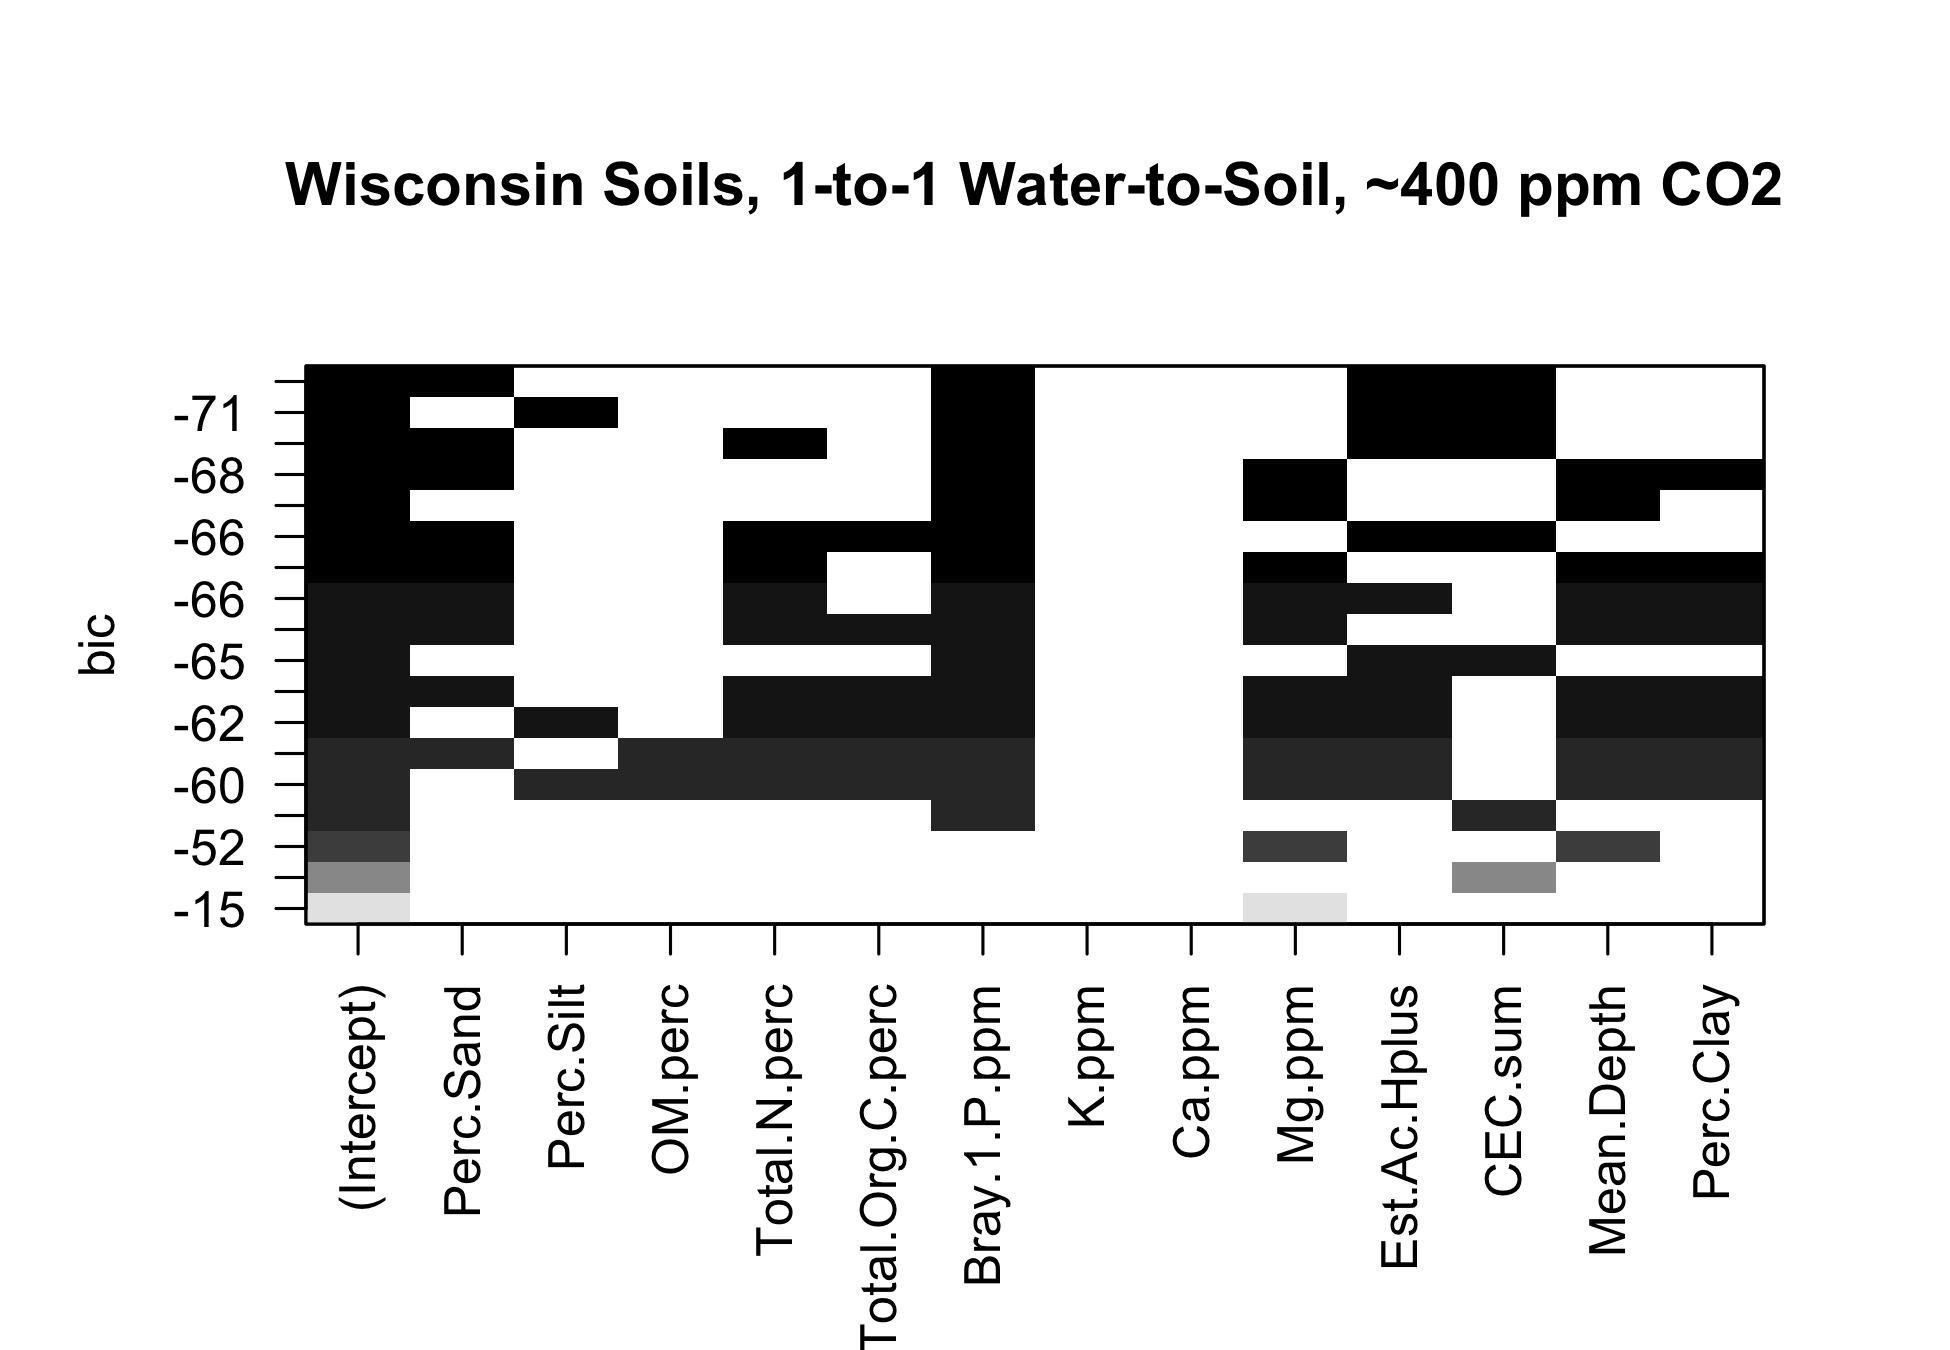
\includegraphics{output-rmd/bic.wisc.one2one.labco2-1.png}

\begin{Shaded}
\begin{Highlighting}[]
\NormalTok{bic.wisc.one2one.highco2 <-}\StringTok{ }\KeywordTok{regsubsets}\NormalTok{(High.CO2.pH }\OperatorTok{~}\StringTok{ }\NormalTok{Perc.Sand }\OperatorTok{+}\StringTok{ }\NormalTok{Perc.Silt }\OperatorTok{+}\StringTok{ }\NormalTok{Perc.Clay }\OperatorTok{+}\StringTok{ }\NormalTok{OM.perc }\OperatorTok{+}\StringTok{ }\NormalTok{Total.N.perc }\OperatorTok{+}\StringTok{ }\NormalTok{Total.Org.C.perc }\OperatorTok{+}\StringTok{ }\NormalTok{Bray.}\FloatTok{1.}\NormalTok{P.ppm }\OperatorTok{+}\StringTok{ }\NormalTok{K.ppm }\OperatorTok{+}\StringTok{ }\NormalTok{Ca.ppm }\OperatorTok{+}\StringTok{ }\NormalTok{Mg.ppm }\OperatorTok{+}\StringTok{ }\NormalTok{Est.Ac.Hplus }\OperatorTok{+}\StringTok{ }\NormalTok{CEC.sum }\OperatorTok{+}\StringTok{ }\NormalTok{Mean.Depth, }\DataTypeTok{nbest =} \DecValTok{2}\NormalTok{,}\DataTypeTok{data =}\NormalTok{ dat.wisc.}\FloatTok{1.}\NormalTok{to}\FloatTok{.1}\NormalTok{)}
\end{Highlighting}
\end{Shaded}

\begin{verbatim}
## Reordering variables and trying again:
\end{verbatim}

\begin{Shaded}
\begin{Highlighting}[]
\KeywordTok{plot}\NormalTok{(bic.wisc.one2one.highco2, }\DataTypeTok{scale=}\StringTok{'bic'}\NormalTok{, }\DataTypeTok{main=}\StringTok{"Wisconsin Soils, 1-to-1 Water-to-Soil, ~2% CO2"}\NormalTok{)}
\end{Highlighting}
\end{Shaded}

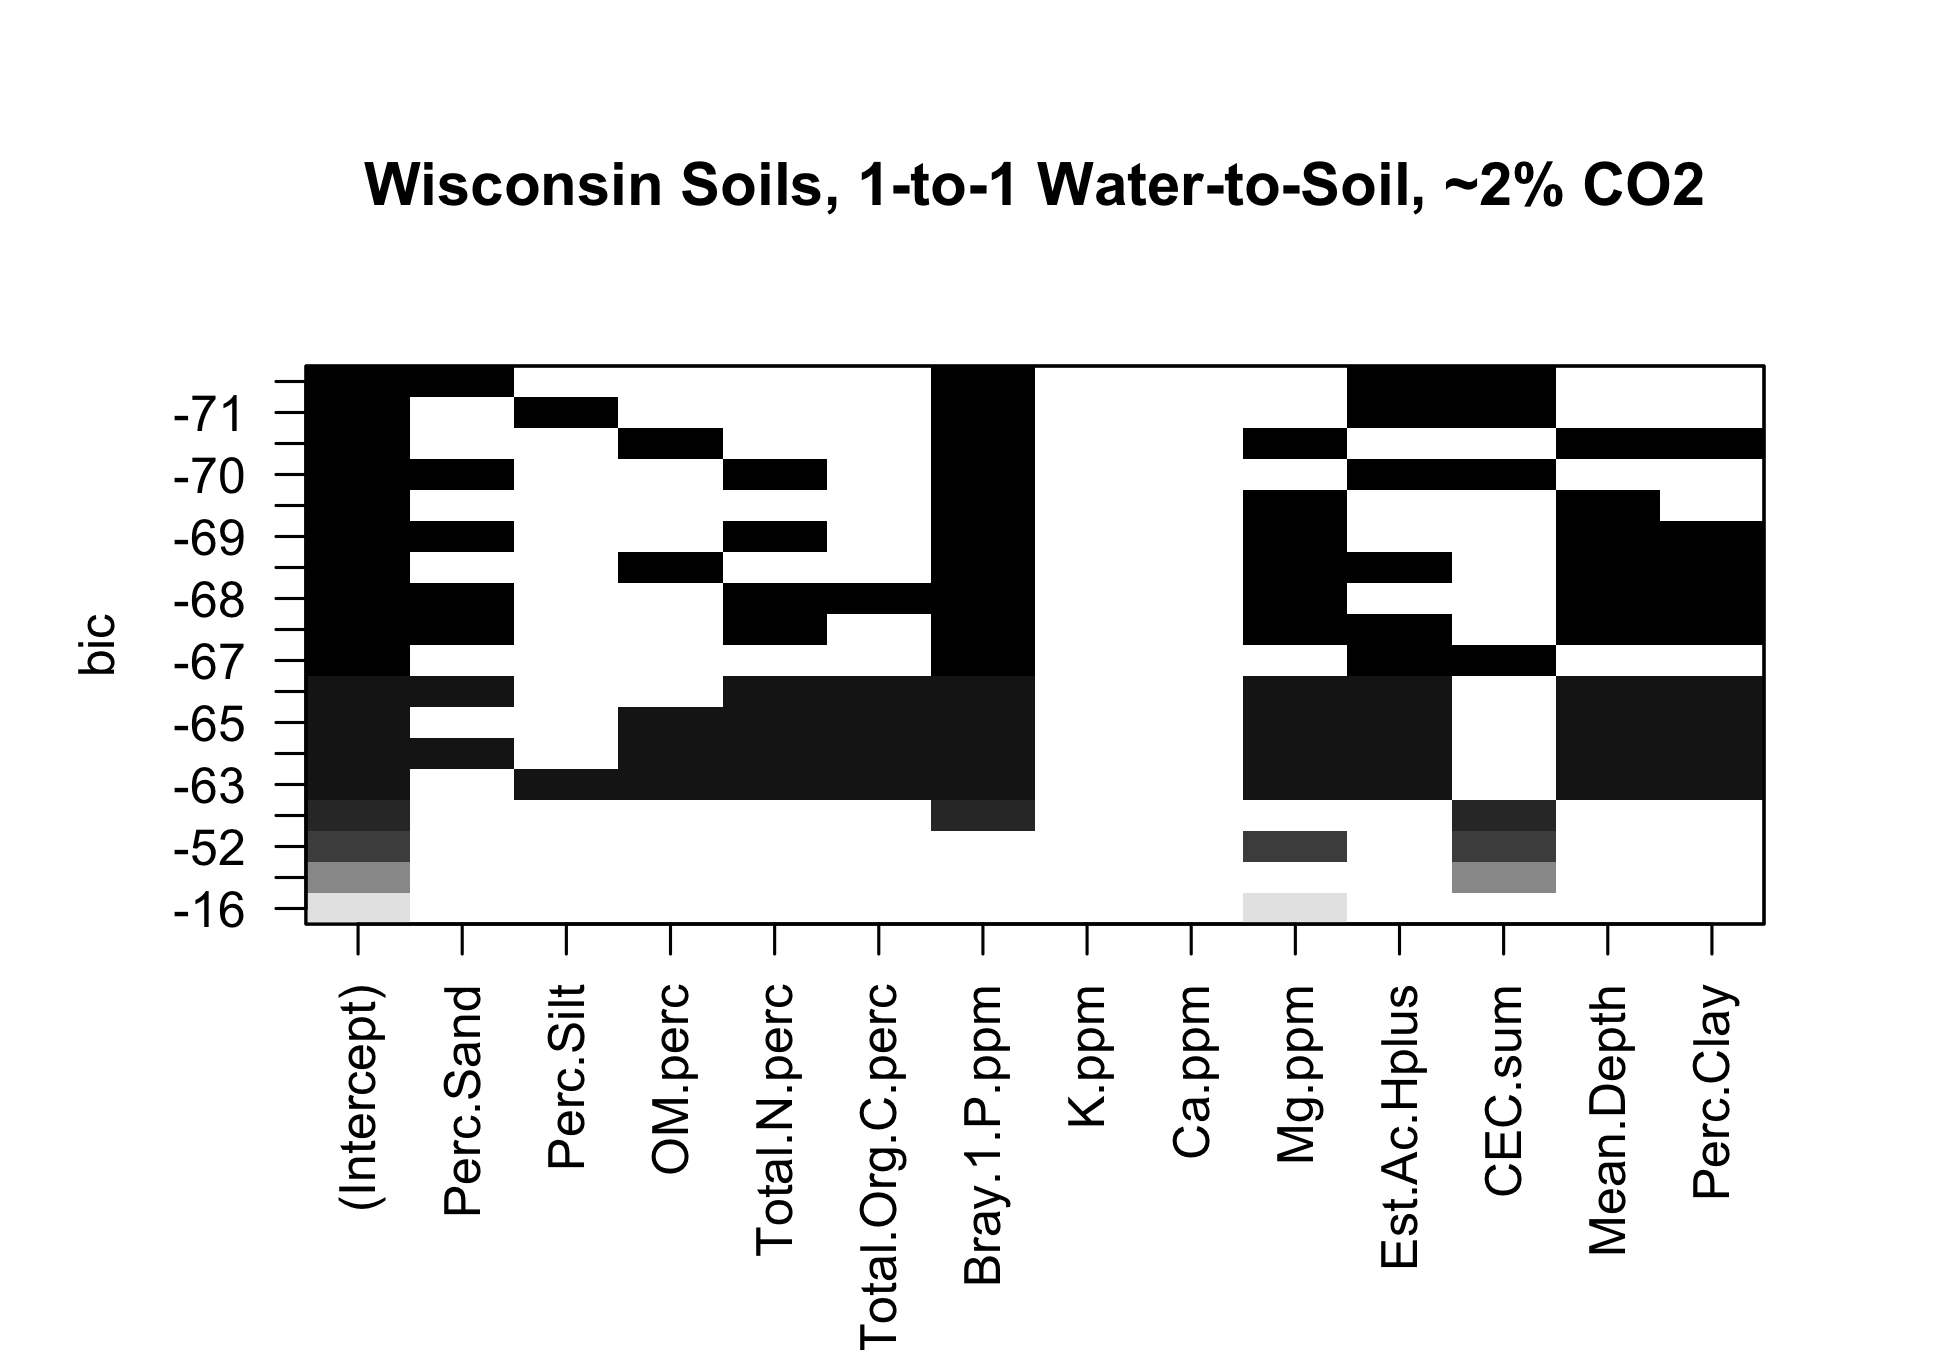
\includegraphics{output-rmd/bic.wisc.one2one.highco2-1.png}

\hypertarget{one2two}{%
\subsubsection{one2two}\label{one2two}}

\begin{Shaded}
\begin{Highlighting}[]
\NormalTok{dat.wisc.}\FloatTok{1.}\NormalTok{to}\FloatTok{.2}\NormalTok{ <-}\StringTok{ }\KeywordTok{subset}\NormalTok{(dat.wisc, Water.Soil.Ratio}\OperatorTok{==}\StringTok{"1-to-2"}\NormalTok{)}
\KeywordTok{str}\NormalTok{(dat.wisc.}\FloatTok{1.}\NormalTok{to}\FloatTok{.2}\NormalTok{)}
\end{Highlighting}
\end{Shaded}

\begin{verbatim}
## 'data.frame':    63 obs. of  47 variables:
##  $ Horizon                  : chr  "Topsoil" "Subsoil" "Subsoil" "Topsoil" ...
##  $ Water.Soil.Ratio         : chr  "1-to-2" "1-to-2" "1-to-2" "1-to-2" ...
##  $ Sample.ID                : chr  "001-K1-0-17" "002-K1-17-45" "003-K1-45-60" "005-K3-0-15" ...
##  $ Study                    : chr  "Wisconsin" "Wisconsin" "Wisconsin" "Wisconsin" ...
##  $ Sample.Number            : int  1 2 3 5 6 7 8 9 10 11 ...
##  $ DNA.Extr.pH.After.C1     : num  8.83 9.12 9.38 8.69 9.03 ...
##  $ DNA.Extr.pH.After.C2     : num  7.78 8 7.98 7.72 7.9 ...
##  $ Lab.CO2.pH               : num  4.87 5.2 5.48 4.99 5.28 5.2 4.87 5.13 5.03 5.53 ...
##  $ High.CO2.pH              : num  4.93 5.33 5.01 5.01 5.22 5.24 4.91 5.1 4.91 5.53 ...
##  $ Tube.Empty.g             : num  1.005 1.008 1.013 0.999 0.999 ...
##  $ Moist.Soil.g             : num  0.946 1.065 1.069 1.053 1.046 ...
##  $ Water.Added.mL           : num  0.473 0.533 0.535 0.527 0.523 0.527 0.472 0.517 0.509 0.508 ...
##  $ Tube.Dry.Soil.g          : num  1.85 1.97 2.03 1.93 1.95 ...
##  $ Dry.Soil.g               : num  0.845 0.964 1.017 0.933 0.947 ...
##  $ Water.Cont.mass          : num  0.107 0.095 0.049 0.114 0.095 0.062 0.06 0.033 0.083 0.032 ...
##  $ Target.Water.Soil.Content: num  0.5 0.5 0.5 0.5 0.5 0.5 0.5 0.5 0.5 0.5 ...
##  $ Real.Water.Soil.ratio    : num  0.56 0.552 0.526 0.564 0.552 0.533 0.532 0.517 0.545 0.517 ...
##  $ Error.Water.Soil.ratio   : num  -0.06 -0.052 -0.026 -0.064 -0.052 -0.033 -0.032 -0.017 -0.045 -0.017 ...
##  $ Perc.Sand                : num  64 68 72 64 60 70 78 74 72 82 ...
##  $ Perc.Silt                : num  25.2 21.2 19.2 27.2 31.2 19.2 15.2 15.2 15.2 11.2 ...
##  $ Perc.Clay                : num  10.8 10.8 8.8 8.8 8.8 10.8 6.8 10.8 12.8 6.8 ...
##  $ Texture.Name             : chr  "Sandy Loam" "Sandy Loam" "Sandy Loam" "Sandy Loam" ...
##  $ OM.perc                  : num  2.5 1.3 0.4 4 1.5 0.8 2.5 1.4 0.8 1.2 ...
##  $ Scoop.Density.g.4.24.cc  : num  4.6 5.36 6.28 4.38 5.05 5.76 4.89 5.44 5.51 6.16 ...
##  $ Soil.pH                  : num  4.9 5.4 5.6 4.7 5.1 5.2 4.5 5 4.4 5.5 ...
##  $ Sikora.pH                : num  6.3 6.5 7.1 6.1 6.4 6.7 6.1 6.4 6.5 6.8 ...
##  $ Total.N.perc             : num  0.13 0.09 0.08 0.18 0.12 0.11 0.13 0.11 0.11 0.13 ...
##  $ Total.Org.C.perc         : num  1.64 0.71 0.11 2.52 0.77 0.33 1.63 0.68 0.34 0.81 ...
##  $ Bray.1.P.ppm             : int  99 101 37 63 40 24 18 64 16 197 ...
##  $ K.ppm                    : int  44 41 26 67 57 63 42 29 23 62 ...
##  $ K.perc.CEC               : int  1 1 4 1 2 3 1 1 1 6 ...
##  $ Ca.ppm                   : int  237 194 327 382 170 189 122 22 22 134 ...
##  $ Ca.perc.CEC              : int  12 13 96 15 11 19 5 1 2 23 ...
##  $ Mg.ppm                   : int  40 32 58 85 39 38 22 6 5 8 ...
##  $ Mg.perc.CEC              : int  3 4 28 5 4 6 2 1 1 2 ...
##  $ Na.ppm                   : logi  NA NA NA NA NA NA ...
##  $ Na.perc.CEC              : int  0 0 0 0 0 0 0 0 0 0 ...
##  $ Est.Ac.Hplus             : num  8.6 6.1 0 10.9 7 4 10.7 7.3 5.5 2 ...
##  $ Hplus.perc.CEC           : int  87 85 0 84 87 78 94 98 97 71 ...
##  $ CEC.sum                  : int  9 6 1 13 7 4 10 6 4 2 ...
##  $ Date.of.Collection       : chr  "8/23/2018" "8/23/2018" "8/23/2018" "8/23/2018" ...
##  $ Station.Name             : chr  "Kemp" "Kemp" "Kemp" "Kemp" ...
##  $ St.pH.WSS                : num  5.4 5.4 5.4 5.4 5.4 5.4 5.4 5.4 5.4 5.5 ...
##  $ Site.Number              : int  1 1 1 3 3 3 4 4 4 1 ...
##  $ Upper.Depth.cm           : int  0 17 45 0 15 35 0 15 30 0 ...
##  $ Lower.Depth.cm           : int  17 45 60 15 35 50 15 30 50 27 ...
##  $ Mean.Depth               : num  8.5 31 52.5 7.5 25 42.5 7.5 22.5 40 13.5 ...
\end{verbatim}

\begin{Shaded}
\begin{Highlighting}[]
\NormalTok{bic.wisc.one2two.labco2 <-}\StringTok{ }\KeywordTok{regsubsets}\NormalTok{(Lab.CO2.pH }\OperatorTok{~}\StringTok{ }\NormalTok{Perc.Sand }\OperatorTok{+}\StringTok{ }\NormalTok{Perc.Silt }\OperatorTok{+}\StringTok{ }\NormalTok{Perc.Clay }\OperatorTok{+}\StringTok{ }\NormalTok{OM.perc }\OperatorTok{+}\StringTok{ }\NormalTok{Total.N.perc }\OperatorTok{+}\StringTok{ }\NormalTok{Total.Org.C.perc }\OperatorTok{+}\StringTok{ }\NormalTok{Bray.}\FloatTok{1.}\NormalTok{P.ppm }\OperatorTok{+}\StringTok{ }\NormalTok{K.ppm }\OperatorTok{+}\StringTok{ }\NormalTok{Ca.ppm }\OperatorTok{+}\StringTok{ }\NormalTok{Mg.ppm }\OperatorTok{+}\StringTok{ }\NormalTok{Est.Ac.Hplus }\OperatorTok{+}\StringTok{ }\NormalTok{CEC.sum }\OperatorTok{+}\StringTok{ }\NormalTok{Mean.Depth, }\DataTypeTok{nbest =} \DecValTok{2}\NormalTok{,}\DataTypeTok{data =}\NormalTok{ dat.wisc.}\FloatTok{1.}\NormalTok{to}\FloatTok{.2}\NormalTok{)}
\end{Highlighting}
\end{Shaded}

\begin{verbatim}
## Reordering variables and trying again:
\end{verbatim}

\begin{Shaded}
\begin{Highlighting}[]
\KeywordTok{plot}\NormalTok{(bic.wisc.one2two.labco2, }\DataTypeTok{scale=}\StringTok{'bic'}\NormalTok{, }\DataTypeTok{main=}\StringTok{"Wisconsin Soils, 1-to-2 Water-to-Soil, ~400 ppm CO2"}\NormalTok{)}
\end{Highlighting}
\end{Shaded}

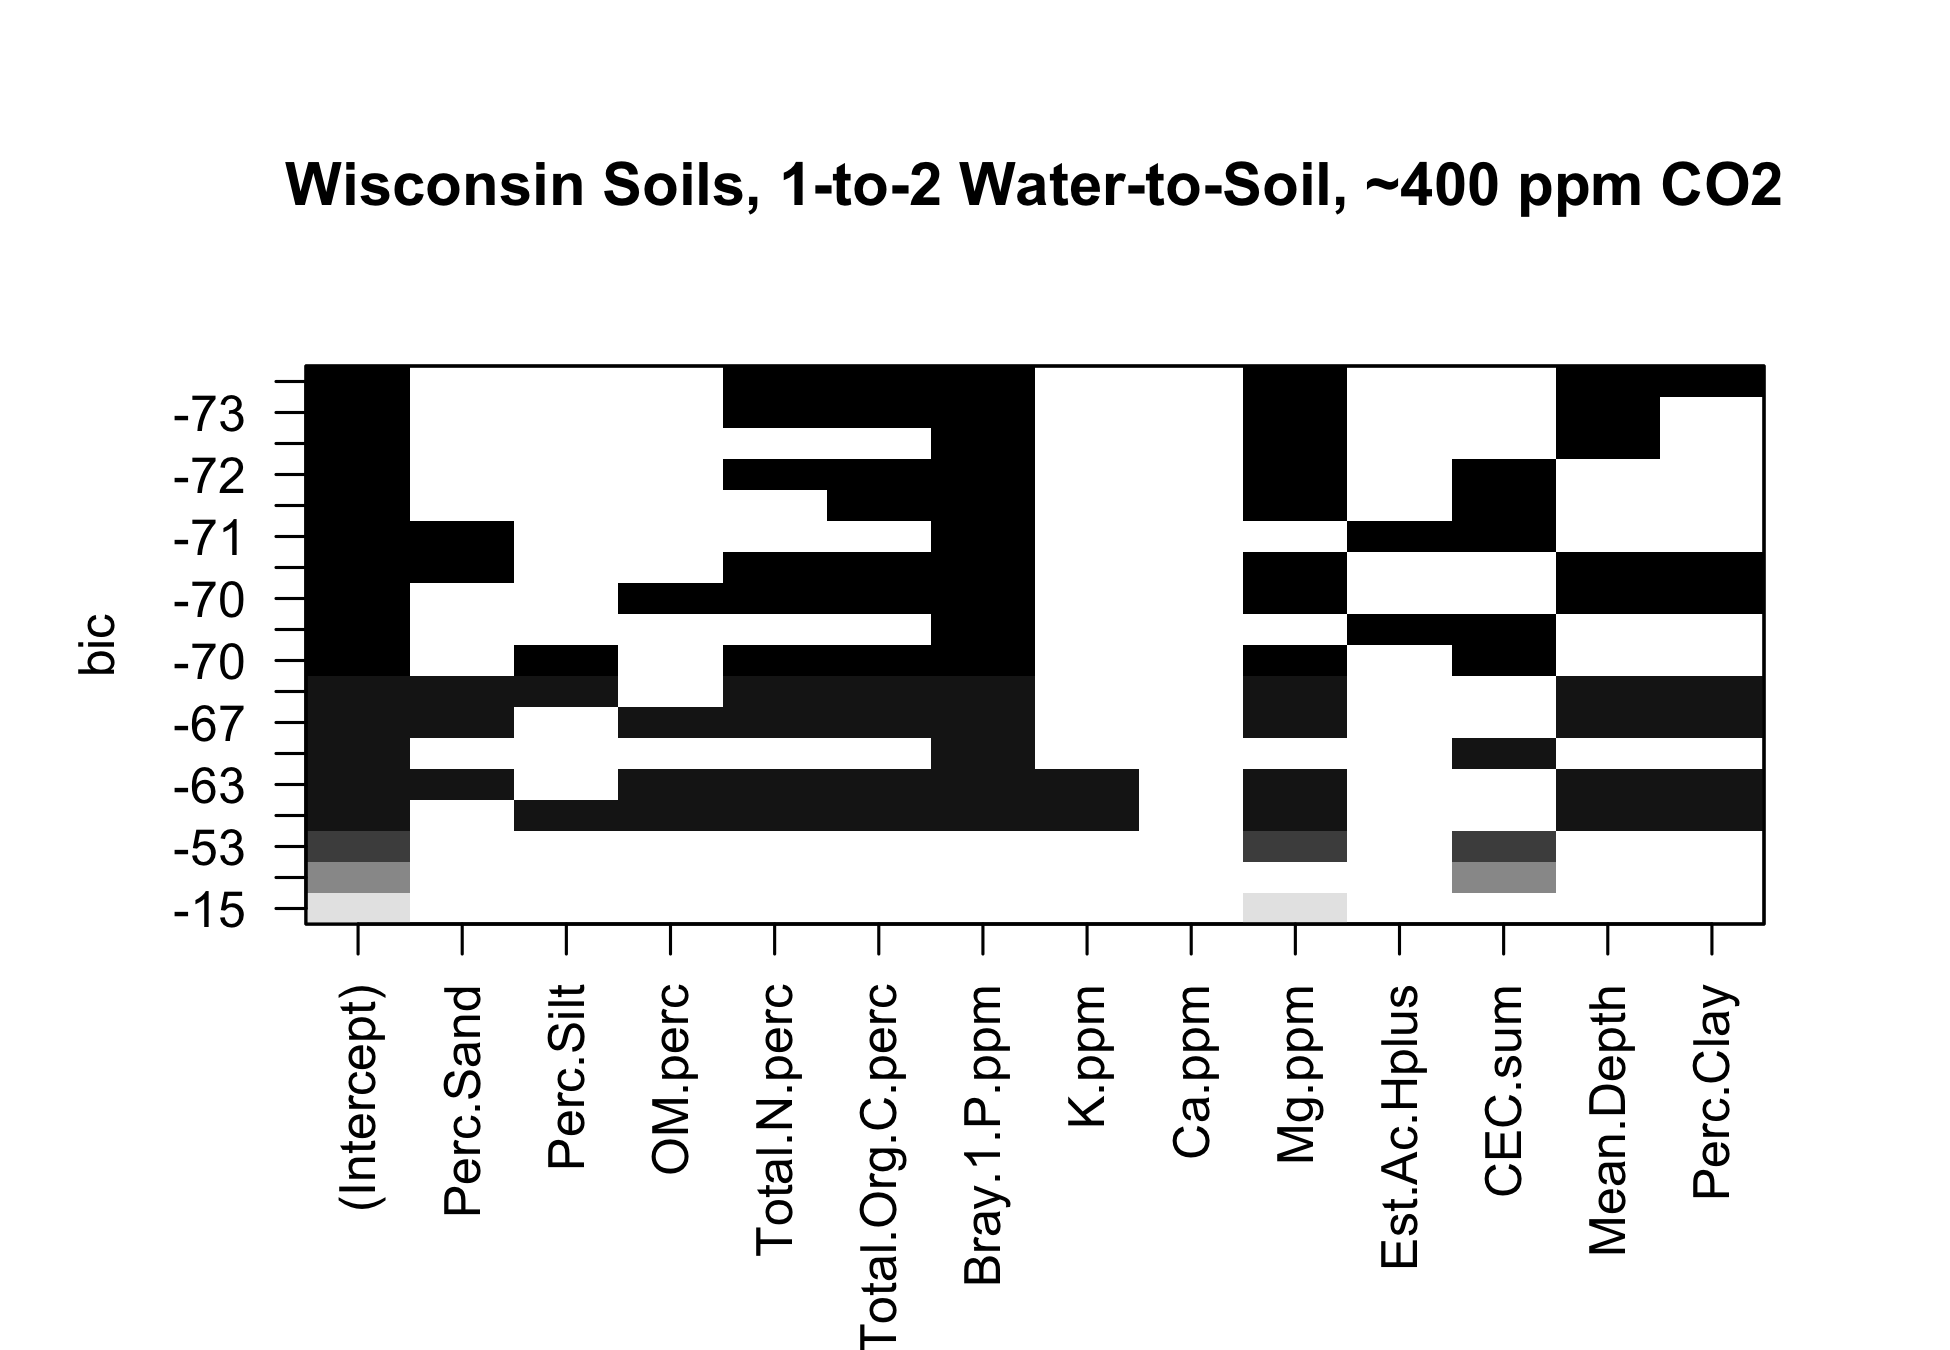
\includegraphics{output-rmd/bic.wisc.one2two.labco2-1.png}

\begin{Shaded}
\begin{Highlighting}[]
\NormalTok{bic.wisc.one2two.highco2 <-}\StringTok{ }\KeywordTok{regsubsets}\NormalTok{(High.CO2.pH }\OperatorTok{~}\StringTok{ }\NormalTok{Perc.Sand }\OperatorTok{+}\StringTok{ }\NormalTok{Perc.Silt }\OperatorTok{+}\StringTok{ }\NormalTok{Perc.Clay }\OperatorTok{+}\StringTok{ }\NormalTok{OM.perc }\OperatorTok{+}\StringTok{ }\NormalTok{Total.N.perc }\OperatorTok{+}\StringTok{ }\NormalTok{Total.Org.C.perc }\OperatorTok{+}\StringTok{ }\NormalTok{Bray.}\FloatTok{1.}\NormalTok{P.ppm }\OperatorTok{+}\StringTok{ }\NormalTok{K.ppm }\OperatorTok{+}\StringTok{ }\NormalTok{Ca.ppm }\OperatorTok{+}\StringTok{ }\NormalTok{Mg.ppm }\OperatorTok{+}\StringTok{ }\NormalTok{Est.Ac.Hplus }\OperatorTok{+}\StringTok{ }\NormalTok{CEC.sum }\OperatorTok{+}\StringTok{ }\NormalTok{Mean.Depth, }\DataTypeTok{nbest =} \DecValTok{2}\NormalTok{, }\DataTypeTok{data =}\NormalTok{ dat.wisc.}\FloatTok{1.}\NormalTok{to}\FloatTok{.2}\NormalTok{)}
\end{Highlighting}
\end{Shaded}

\begin{verbatim}
## Reordering variables and trying again:
\end{verbatim}

\begin{Shaded}
\begin{Highlighting}[]
\KeywordTok{plot}\NormalTok{(bic.wisc.one2two.highco2, }\DataTypeTok{scale=}\StringTok{'bic'}\NormalTok{, }\DataTypeTok{main=}\StringTok{"Wisconsin Soils, 1-to-2 Water-to-Soil, ~2% CO2"}\NormalTok{)}
\end{Highlighting}
\end{Shaded}

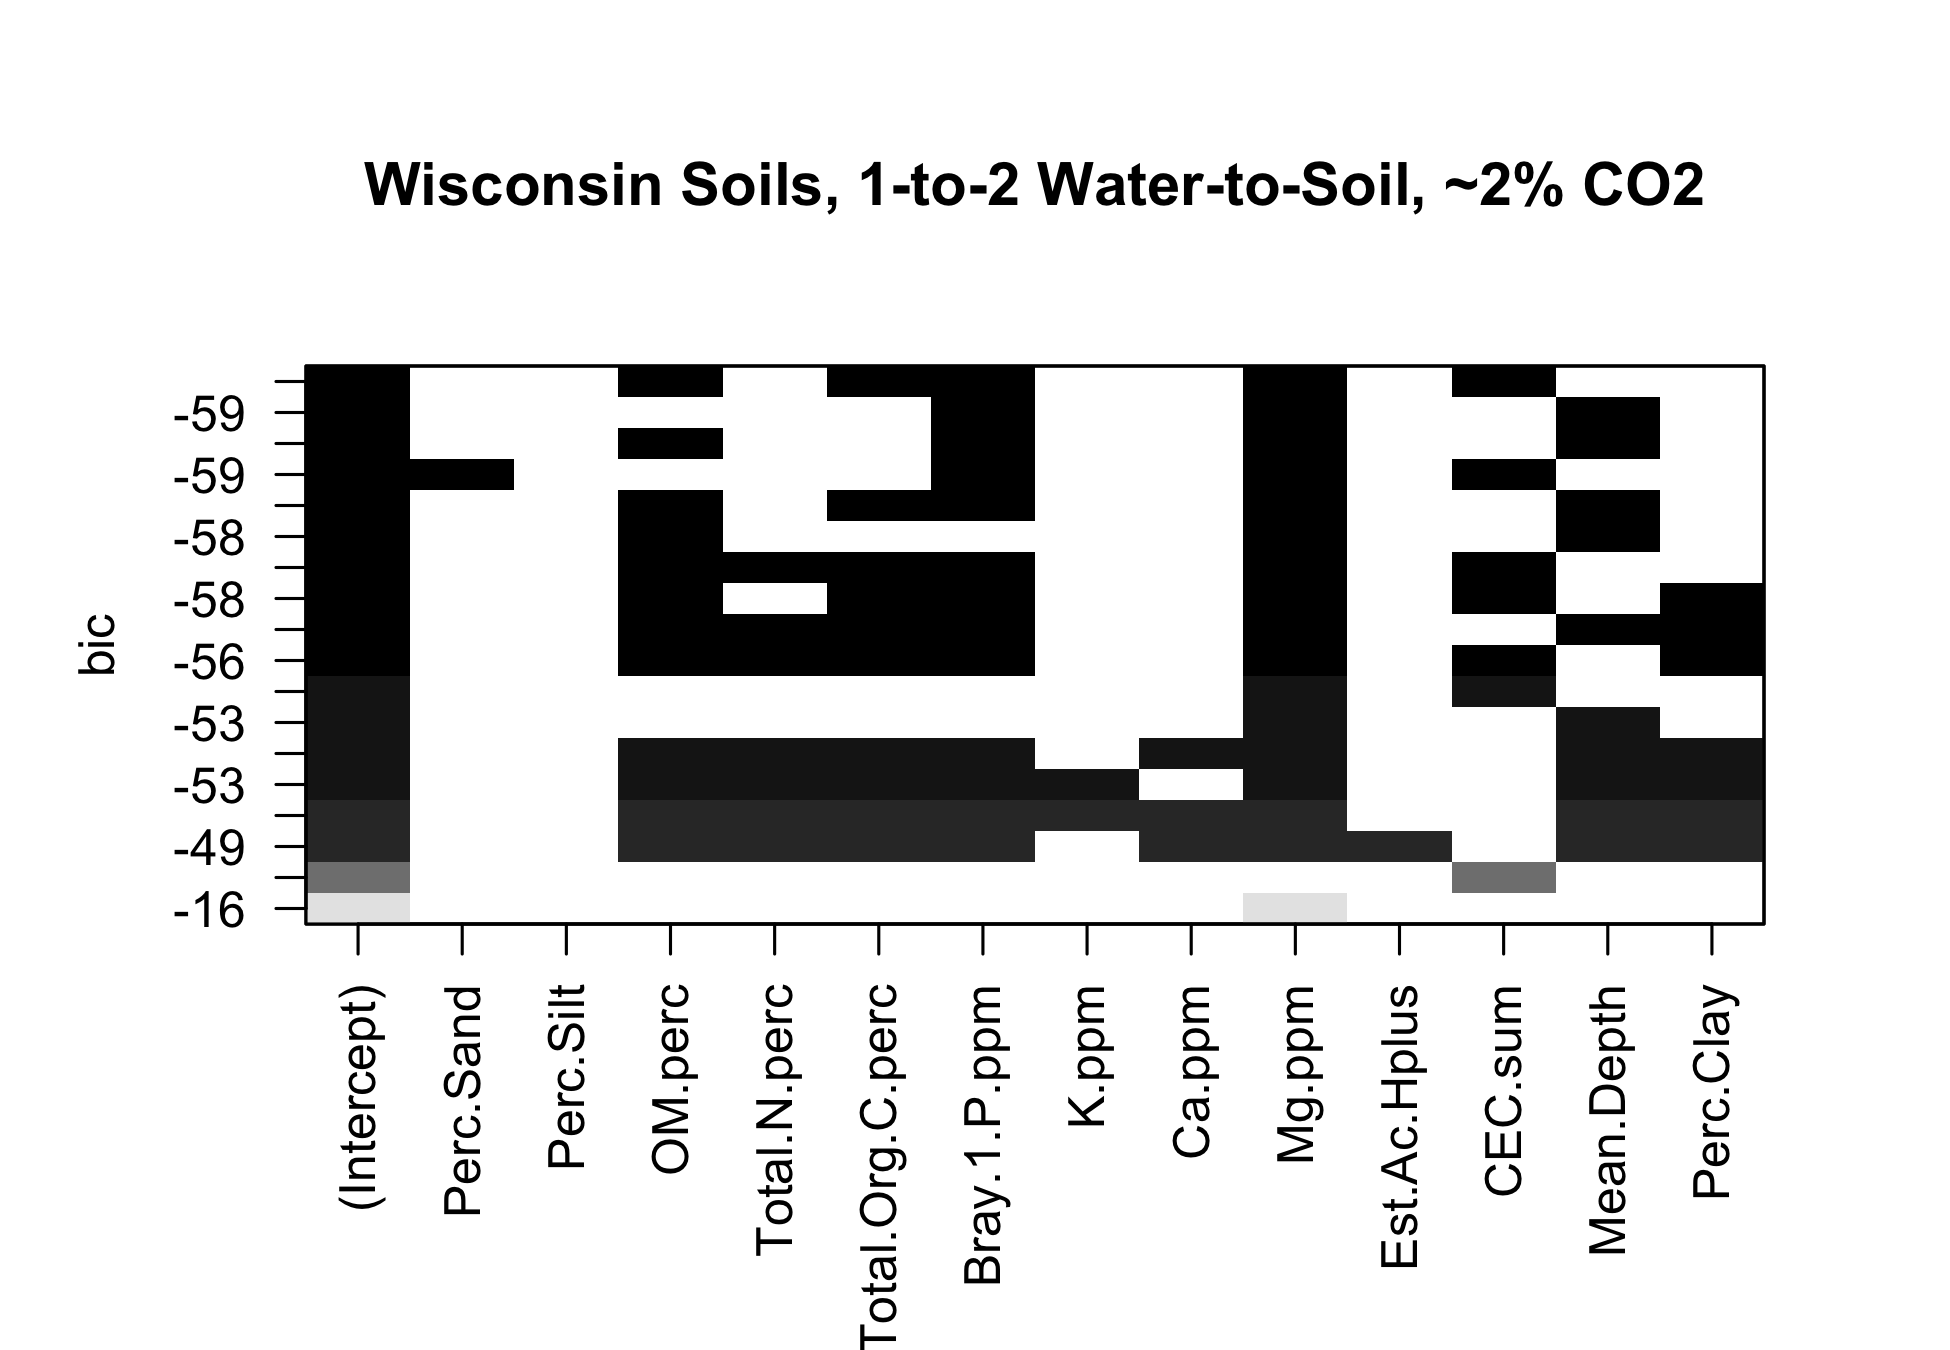
\includegraphics{output-rmd/bic.wisc.one2two.highco2-1.png}

\hypertarget{one2three}{%
\subsubsection{one2three}\label{one2three}}

\begin{Shaded}
\begin{Highlighting}[]
\NormalTok{dat.wisc.}\FloatTok{1.}\NormalTok{to}\FloatTok{.3}\NormalTok{ <-}\StringTok{ }\KeywordTok{subset}\NormalTok{(dat.wisc, Water.Soil.Ratio}\OperatorTok{==}\StringTok{"1-to-3"}\NormalTok{)}
\KeywordTok{str}\NormalTok{(dat.wisc.}\FloatTok{1.}\NormalTok{to}\FloatTok{.3}\NormalTok{)}
\end{Highlighting}
\end{Shaded}

\begin{verbatim}
## 'data.frame':    63 obs. of  47 variables:
##  $ Horizon                  : chr  "Topsoil" "Subsoil" "Subsoil" "Topsoil" ...
##  $ Water.Soil.Ratio         : chr  "1-to-3" "1-to-3" "1-to-3" "1-to-3" ...
##  $ Sample.ID                : chr  "001-K1-0-17" "002-K1-17-45" "003-K1-45-60" "005-K3-0-15" ...
##  $ Study                    : chr  "Wisconsin" "Wisconsin" "Wisconsin" "Wisconsin" ...
##  $ Sample.Number            : int  1 2 3 5 6 7 8 9 10 11 ...
##  $ DNA.Extr.pH.After.C1     : num  8.83 9.12 9.38 8.69 9.03 ...
##  $ DNA.Extr.pH.After.C2     : num  7.78 8 7.98 7.72 7.9 ...
##  $ Lab.CO2.pH               : num  5.08 5.34 5.41 5.01 5.16 5.13 4.77 5.06 4.99 5.44 ...
##  $ High.CO2.pH              : num  5.15 5.44 5.57 5.12 5.3 5.25 4.94 5.13 5.11 5.68 ...
##  $ Tube.Empty.g             : num  1.066 0.016 1.059 1.068 1.058 ...
##  $ Moist.Soil.g             : num  1.18 1.23 1.25 1.24 1.22 ...
##  $ Water.Added.mL           : num  0.392 0.41 0.415 0.413 0.405 0.413 0.397 0.414 0.414 0.399 ...
##  $ Tube.Dry.Soil.g          : num  2.13 2.19 2.25 2.22 2.16 ...
##  $ Dry.Soil.g               : num  1.07 2.17 1.19 1.15 1.1 ...
##  $ Water.Cont.mass          : num  0.091 -0.768 0.045 0.072 0.095 0.061 0.064 0.061 0.052 0.034 ...
##  $ Target.Water.Soil.Content: num  0.333 0.333 0.333 0.333 0.333 0.333 0.333 0.333 0.333 0.333 ...
##  $ Real.Water.Soil.ratio    : num  0.367 0.189 0.349 0.359 0.368 0.355 0.356 0.355 0.351 0.345 ...
##  $ Error.Water.Soil.ratio   : num  -0.033 0.145 -0.016 -0.026 -0.035 -0.022 -0.023 -0.022 -0.018 -0.012 ...
##  $ Perc.Sand                : num  64 68 72 64 60 70 78 74 72 82 ...
##  $ Perc.Silt                : num  25.2 21.2 19.2 27.2 31.2 19.2 15.2 15.2 15.2 11.2 ...
##  $ Perc.Clay                : num  10.8 10.8 8.8 8.8 8.8 10.8 6.8 10.8 12.8 6.8 ...
##  $ Texture.Name             : chr  "Sandy Loam" "Sandy Loam" "Sandy Loam" "Sandy Loam" ...
##  $ OM.perc                  : num  2.5 1.3 0.4 4 1.5 0.8 2.5 1.4 0.8 1.2 ...
##  $ Scoop.Density.g.4.24.cc  : num  4.6 5.36 6.28 4.38 5.05 5.76 4.89 5.44 5.51 6.16 ...
##  $ Soil.pH                  : num  4.9 5.4 5.6 4.7 5.1 5.2 4.5 5 4.4 5.5 ...
##  $ Sikora.pH                : num  6.3 6.5 7.1 6.1 6.4 6.7 6.1 6.4 6.5 6.8 ...
##  $ Total.N.perc             : num  0.13 0.09 0.08 0.18 0.12 0.11 0.13 0.11 0.11 0.13 ...
##  $ Total.Org.C.perc         : num  1.64 0.71 0.11 2.52 0.77 0.33 1.63 0.68 0.34 0.81 ...
##  $ Bray.1.P.ppm             : int  99 101 37 63 40 24 18 64 16 197 ...
##  $ K.ppm                    : int  44 41 26 67 57 63 42 29 23 62 ...
##  $ K.perc.CEC               : int  1 1 4 1 2 3 1 1 1 6 ...
##  $ Ca.ppm                   : int  237 194 327 382 170 189 122 22 22 134 ...
##  $ Ca.perc.CEC              : int  12 13 96 15 11 19 5 1 2 23 ...
##  $ Mg.ppm                   : int  40 32 58 85 39 38 22 6 5 8 ...
##  $ Mg.perc.CEC              : int  3 4 28 5 4 6 2 1 1 2 ...
##  $ Na.ppm                   : logi  NA NA NA NA NA NA ...
##  $ Na.perc.CEC              : int  0 0 0 0 0 0 0 0 0 0 ...
##  $ Est.Ac.Hplus             : num  8.6 6.1 0 10.9 7 4 10.7 7.3 5.5 2 ...
##  $ Hplus.perc.CEC           : int  87 85 0 84 87 78 94 98 97 71 ...
##  $ CEC.sum                  : int  9 6 1 13 7 4 10 6 4 2 ...
##  $ Date.of.Collection       : chr  "8/23/2018" "8/23/2018" "8/23/2018" "8/23/2018" ...
##  $ Station.Name             : chr  "Kemp" "Kemp" "Kemp" "Kemp" ...
##  $ St.pH.WSS                : num  5.4 5.4 5.4 5.4 5.4 5.4 5.4 5.4 5.4 5.5 ...
##  $ Site.Number              : int  1 1 1 3 3 3 4 4 4 1 ...
##  $ Upper.Depth.cm           : int  0 17 45 0 15 35 0 15 30 0 ...
##  $ Lower.Depth.cm           : int  17 45 60 15 35 50 15 30 50 27 ...
##  $ Mean.Depth               : num  8.5 31 52.5 7.5 25 42.5 7.5 22.5 40 13.5 ...
\end{verbatim}

\begin{Shaded}
\begin{Highlighting}[]
\NormalTok{bic.wisc.one2three.labco2 <-}\StringTok{ }\KeywordTok{regsubsets}\NormalTok{(Lab.CO2.pH }\OperatorTok{~}\StringTok{ }\NormalTok{Perc.Sand }\OperatorTok{+}\StringTok{ }\NormalTok{Perc.Silt }\OperatorTok{+}\StringTok{ }\NormalTok{Perc.Clay }\OperatorTok{+}\StringTok{ }\NormalTok{OM.perc }\OperatorTok{+}\StringTok{ }\NormalTok{Total.N.perc }\OperatorTok{+}\StringTok{ }\NormalTok{Total.Org.C.perc }\OperatorTok{+}\StringTok{ }\NormalTok{Bray.}\FloatTok{1.}\NormalTok{P.ppm }\OperatorTok{+}\StringTok{ }\NormalTok{K.ppm }\OperatorTok{+}\StringTok{ }\NormalTok{Ca.ppm }\OperatorTok{+}\StringTok{ }\NormalTok{Mg.ppm }\OperatorTok{+}\StringTok{ }\NormalTok{Est.Ac.Hplus }\OperatorTok{+}\StringTok{ }\NormalTok{CEC.sum }\OperatorTok{+}\StringTok{ }\NormalTok{Mean.Depth, }\DataTypeTok{nbest =} \DecValTok{2}\NormalTok{,}\DataTypeTok{data =}\NormalTok{ dat.wisc.}\FloatTok{1.}\NormalTok{to}\FloatTok{.3}\NormalTok{)}
\end{Highlighting}
\end{Shaded}

\begin{verbatim}
## Reordering variables and trying again:
\end{verbatim}

\begin{Shaded}
\begin{Highlighting}[]
\KeywordTok{plot}\NormalTok{(bic.wisc.one2three.labco2, }\DataTypeTok{scale=}\StringTok{'bic'}\NormalTok{, }\DataTypeTok{main=}\StringTok{"Wisconsin Soils, 1-to-3 Water-to-Soil, ~400 ppm CO2"}\NormalTok{)}
\end{Highlighting}
\end{Shaded}

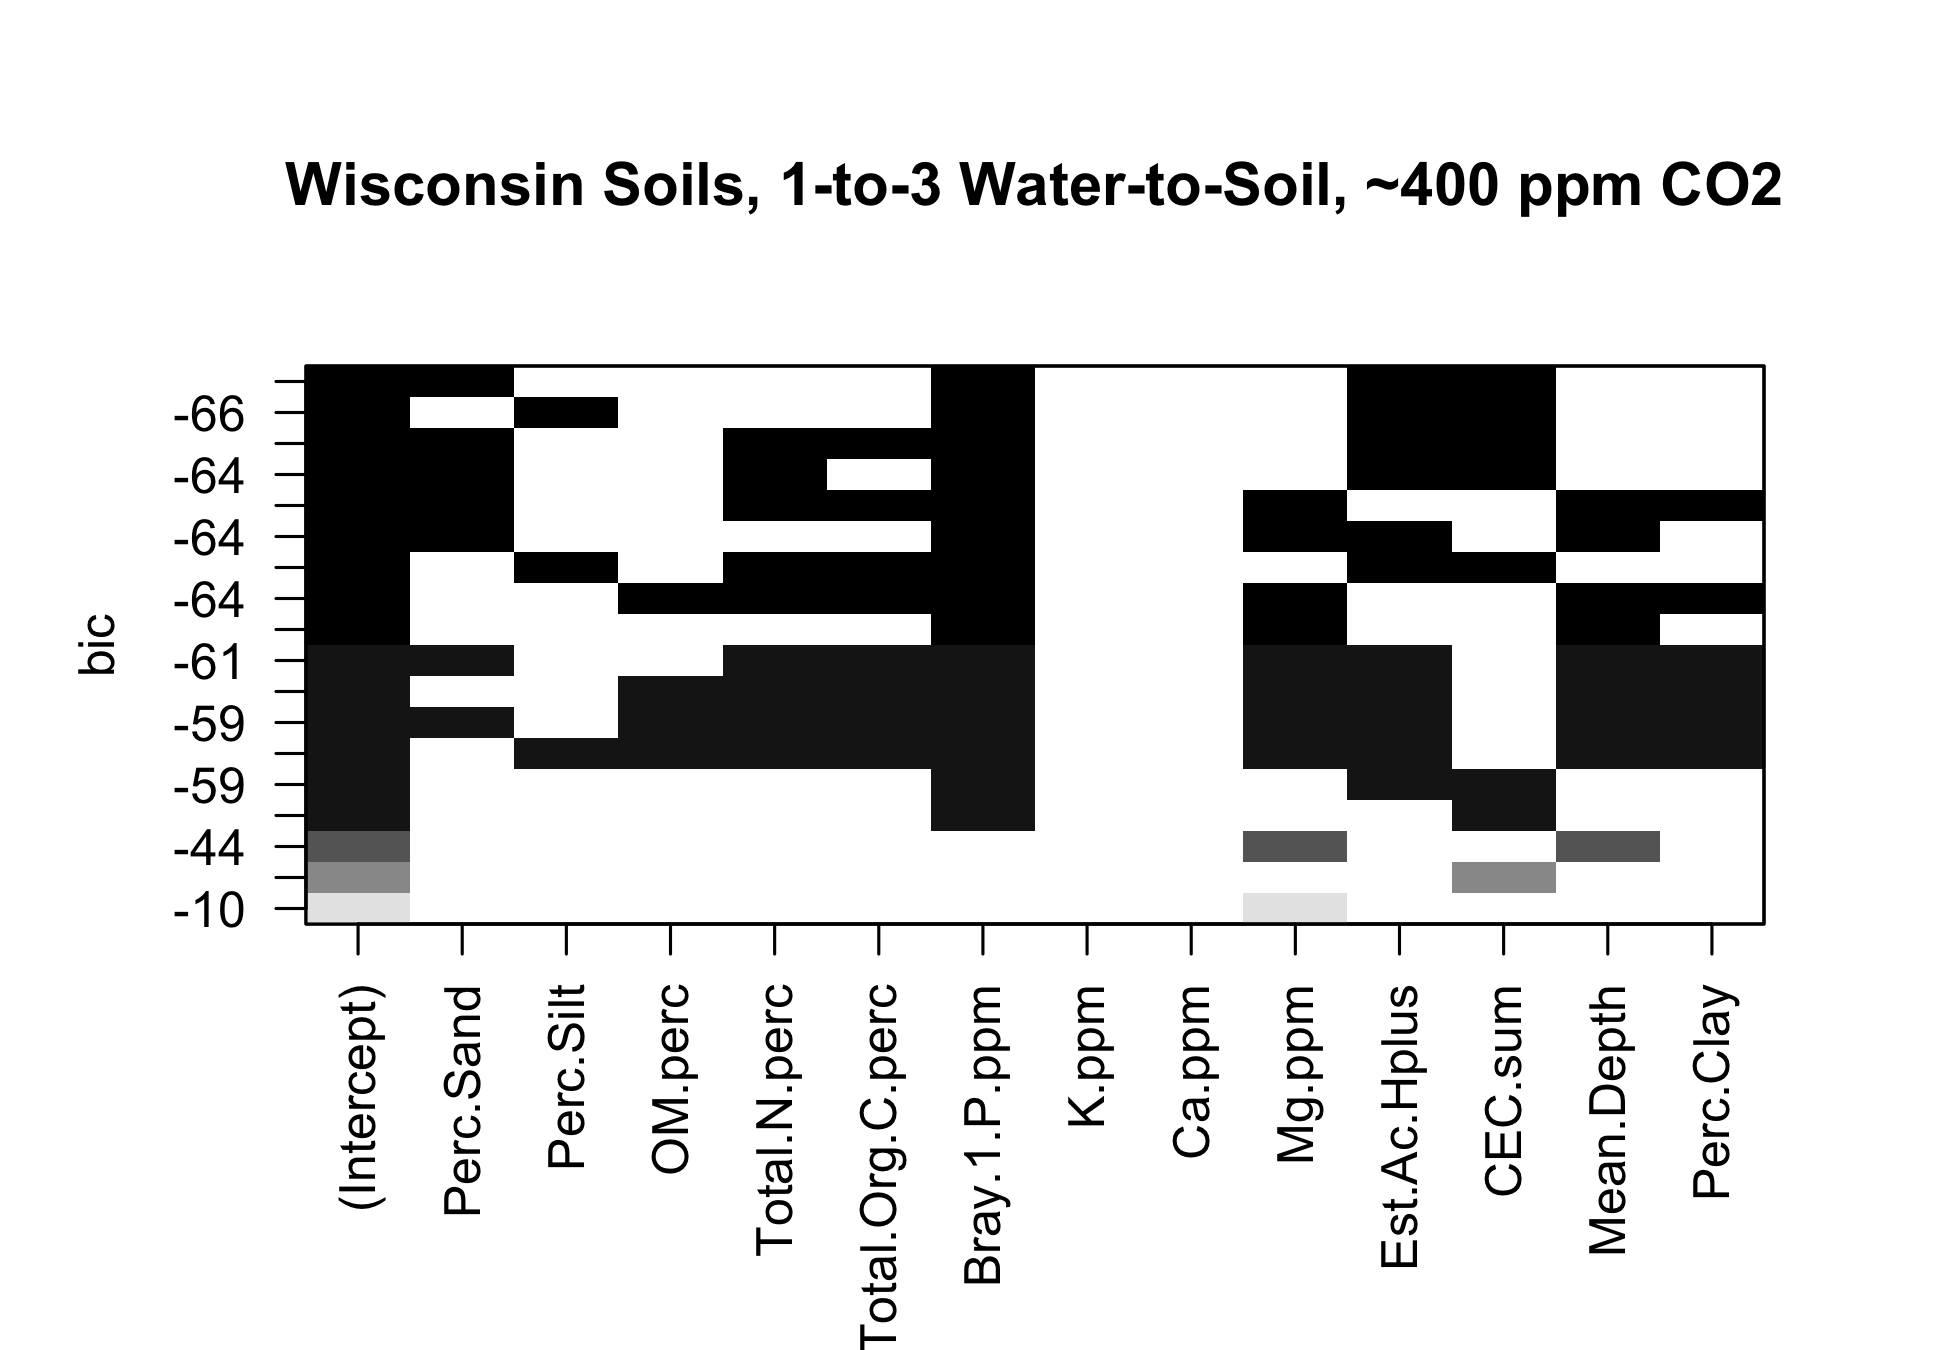
\includegraphics{output-rmd/bic.wisc.one2three.labco2-1.png}

\begin{Shaded}
\begin{Highlighting}[]
\NormalTok{bic.wisc.one2three.labco2 <-}\StringTok{ }\KeywordTok{regsubsets}\NormalTok{(High.CO2.pH }\OperatorTok{~}\StringTok{ }\NormalTok{Perc.Sand }\OperatorTok{+}\StringTok{ }\NormalTok{Perc.Silt }\OperatorTok{+}\StringTok{ }\NormalTok{Perc.Clay }\OperatorTok{+}\StringTok{ }\NormalTok{OM.perc }\OperatorTok{+}\StringTok{ }\NormalTok{Total.N.perc }\OperatorTok{+}\StringTok{ }\NormalTok{Total.Org.C.perc }\OperatorTok{+}\StringTok{ }\NormalTok{Bray.}\FloatTok{1.}\NormalTok{P.ppm }\OperatorTok{+}\StringTok{ }\NormalTok{K.ppm }\OperatorTok{+}\StringTok{ }\NormalTok{Ca.ppm }\OperatorTok{+}\StringTok{ }\NormalTok{Mg.ppm }\OperatorTok{+}\StringTok{ }\NormalTok{Est.Ac.Hplus }\OperatorTok{+}\StringTok{ }\NormalTok{CEC.sum }\OperatorTok{+}\StringTok{ }\NormalTok{Mean.Depth, }\DataTypeTok{nbest =} \DecValTok{2}\NormalTok{,}\DataTypeTok{data =}\NormalTok{ dat.wisc.}\FloatTok{1.}\NormalTok{to}\FloatTok{.3}\NormalTok{)}
\end{Highlighting}
\end{Shaded}

\begin{verbatim}
## Reordering variables and trying again:
\end{verbatim}

\begin{Shaded}
\begin{Highlighting}[]
\KeywordTok{plot}\NormalTok{(bic.wisc.one2three.labco2, }\DataTypeTok{scale=}\StringTok{'bic'}\NormalTok{, }\DataTypeTok{main=}\StringTok{"Wisconsin Soils, 1-to-3 Water-to-Soil, ~2% CO2"}\NormalTok{)}
\end{Highlighting}
\end{Shaded}

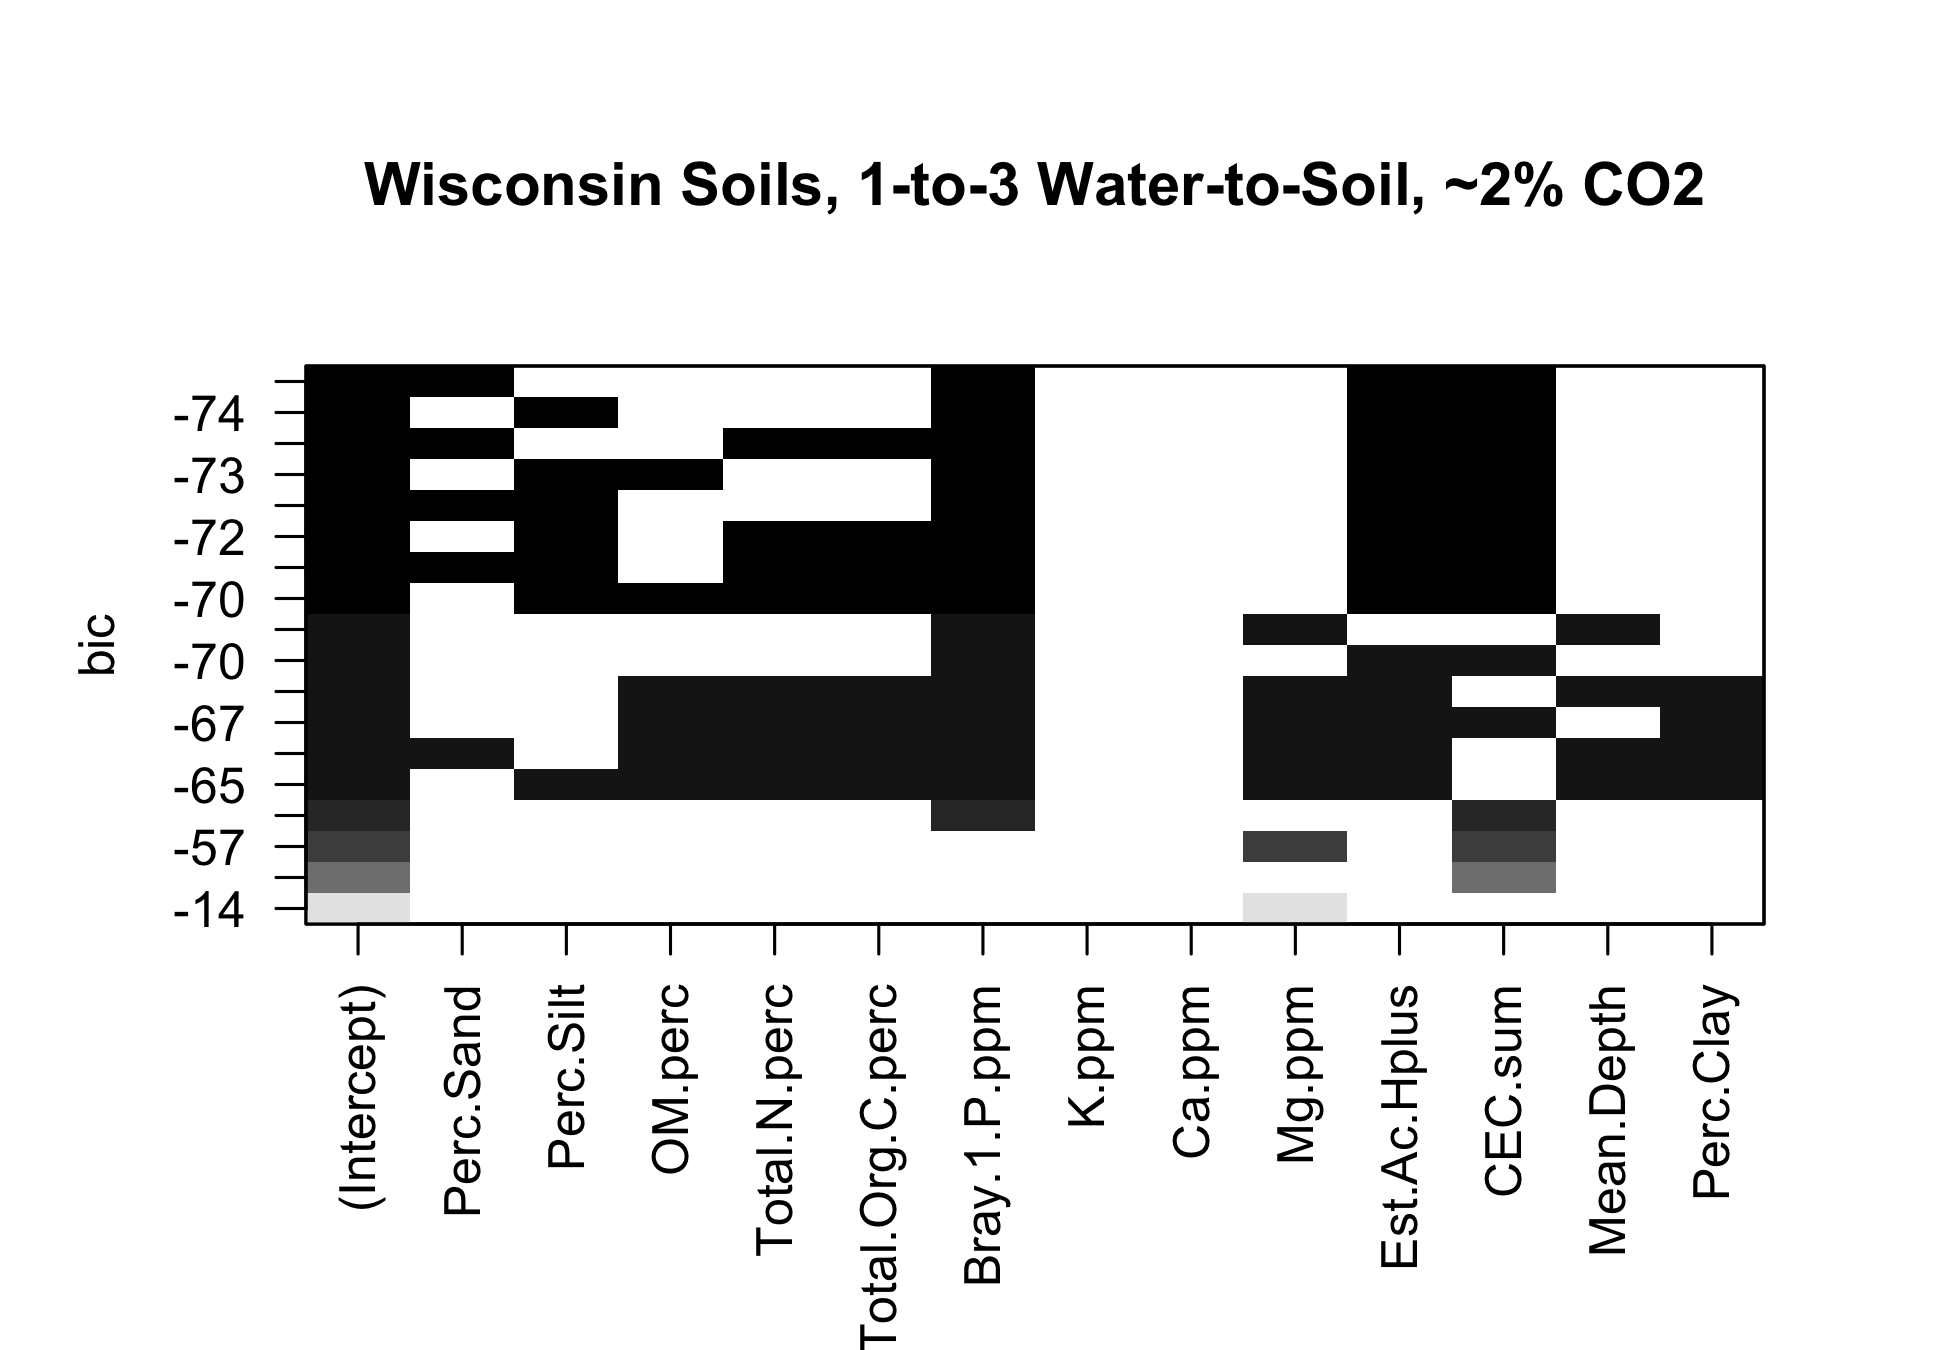
\includegraphics{output-rmd/bic.wisc.one2three.highco2-1.png}

\hypertarget{one2four}{%
\subsubsection{one2four}\label{one2four}}

\begin{Shaded}
\begin{Highlighting}[]
\NormalTok{dat.wisc.}\FloatTok{1.}\NormalTok{to}\FloatTok{.4}\NormalTok{ <-}\StringTok{ }\KeywordTok{subset}\NormalTok{(dat.wisc, Water.Soil.Ratio}\OperatorTok{==}\StringTok{"1-to-4"}\NormalTok{)}
\KeywordTok{str}\NormalTok{(dat.wisc.}\FloatTok{1.}\NormalTok{to}\FloatTok{.4}\NormalTok{)}
\end{Highlighting}
\end{Shaded}

\begin{verbatim}
## 'data.frame':    63 obs. of  47 variables:
##  $ Horizon                  : chr  "Topsoil" "Subsoil" "Subsoil" "Topsoil" ...
##  $ Water.Soil.Ratio         : chr  "1-to-4" "1-to-4" "1-to-4" "1-to-4" ...
##  $ Sample.ID                : chr  "001-K1-0-17" "002-K1-17-45" "003-K1-45-60" "005-K3-0-15" ...
##  $ Study                    : chr  "Wisconsin" "Wisconsin" "Wisconsin" "Wisconsin" ...
##  $ Sample.Number            : int  1 2 3 5 6 7 8 9 10 11 ...
##  $ DNA.Extr.pH.After.C1     : num  8.83 9.12 9.38 8.69 9.03 ...
##  $ DNA.Extr.pH.After.C2     : num  7.78 8 7.98 7.72 7.9 ...
##  $ Lab.CO2.pH               : num  NA 5.22 5.27 NA 4.98 4.99 NA 5.06 4.83 NA ...
##  $ High.CO2.pH              : num  NA 5.36 5.49 NA 5.28 5.28 NA 5.27 5.05 NA ...
##  $ Tube.Empty.g             : num  1.04 1.04 1.02 1.06 1.04 ...
##  $ Moist.Soil.g             : num  1.56 1.61 1.7 1.55 1.61 ...
##  $ Water.Added.mL           : num  0.39 0.404 0.425 0.388 0.404 0.411 0.394 0.407 0.421 0.403 ...
##  $ Tube.Dry.Soil.g          : num  2.44 2.51 2.64 2.41 2.51 ...
##  $ Dry.Soil.g               : num  1.4 1.47 1.62 1.35 1.46 ...
##  $ Water.Cont.mass          : num  0.1 0.089 0.048 0.128 0.095 0.069 0.06 0.058 0.056 0.031 ...
##  $ Target.Water.Soil.Content: num  0.25 0.25 0.25 0.25 0.25 0.25 0.25 0.25 0.25 0.25 ...
##  $ Real.Water.Soil.ratio    : num  0.278 0.274 0.263 0.287 0.276 0.268 0.266 0.265 0.265 0.258 ...
##  $ Error.Water.Soil.ratio   : num  -0.028 -0.024 -0.013 -0.037 -0.026 -0.018 -0.016 -0.015 -0.015 -0.008 ...
##  $ Perc.Sand                : num  64 68 72 64 60 70 78 74 72 82 ...
##  $ Perc.Silt                : num  25.2 21.2 19.2 27.2 31.2 19.2 15.2 15.2 15.2 11.2 ...
##  $ Perc.Clay                : num  10.8 10.8 8.8 8.8 8.8 10.8 6.8 10.8 12.8 6.8 ...
##  $ Texture.Name             : chr  "Sandy Loam" "Sandy Loam" "Sandy Loam" "Sandy Loam" ...
##  $ OM.perc                  : num  2.5 1.3 0.4 4 1.5 0.8 2.5 1.4 0.8 1.2 ...
##  $ Scoop.Density.g.4.24.cc  : num  4.6 5.36 6.28 4.38 5.05 5.76 4.89 5.44 5.51 6.16 ...
##  $ Soil.pH                  : num  4.9 5.4 5.6 4.7 5.1 5.2 4.5 5 4.4 5.5 ...
##  $ Sikora.pH                : num  6.3 6.5 7.1 6.1 6.4 6.7 6.1 6.4 6.5 6.8 ...
##  $ Total.N.perc             : num  0.13 0.09 0.08 0.18 0.12 0.11 0.13 0.11 0.11 0.13 ...
##  $ Total.Org.C.perc         : num  1.64 0.71 0.11 2.52 0.77 0.33 1.63 0.68 0.34 0.81 ...
##  $ Bray.1.P.ppm             : int  99 101 37 63 40 24 18 64 16 197 ...
##  $ K.ppm                    : int  44 41 26 67 57 63 42 29 23 62 ...
##  $ K.perc.CEC               : int  1 1 4 1 2 3 1 1 1 6 ...
##  $ Ca.ppm                   : int  237 194 327 382 170 189 122 22 22 134 ...
##  $ Ca.perc.CEC              : int  12 13 96 15 11 19 5 1 2 23 ...
##  $ Mg.ppm                   : int  40 32 58 85 39 38 22 6 5 8 ...
##  $ Mg.perc.CEC              : int  3 4 28 5 4 6 2 1 1 2 ...
##  $ Na.ppm                   : logi  NA NA NA NA NA NA ...
##  $ Na.perc.CEC              : int  0 0 0 0 0 0 0 0 0 0 ...
##  $ Est.Ac.Hplus             : num  8.6 6.1 0 10.9 7 4 10.7 7.3 5.5 2 ...
##  $ Hplus.perc.CEC           : int  87 85 0 84 87 78 94 98 97 71 ...
##  $ CEC.sum                  : int  9 6 1 13 7 4 10 6 4 2 ...
##  $ Date.of.Collection       : chr  "8/23/2018" "8/23/2018" "8/23/2018" "8/23/2018" ...
##  $ Station.Name             : chr  "Kemp" "Kemp" "Kemp" "Kemp" ...
##  $ St.pH.WSS                : num  5.4 5.4 5.4 5.4 5.4 5.4 5.4 5.4 5.4 5.5 ...
##  $ Site.Number              : int  1 1 1 3 3 3 4 4 4 1 ...
##  $ Upper.Depth.cm           : int  0 17 45 0 15 35 0 15 30 0 ...
##  $ Lower.Depth.cm           : int  17 45 60 15 35 50 15 30 50 27 ...
##  $ Mean.Depth               : num  8.5 31 52.5 7.5 25 42.5 7.5 22.5 40 13.5 ...
\end{verbatim}

\begin{Shaded}
\begin{Highlighting}[]
\NormalTok{bic.wisc.one2four.labco2 <-}\StringTok{ }\KeywordTok{regsubsets}\NormalTok{(Lab.CO2.pH }\OperatorTok{~}\StringTok{ }\NormalTok{Perc.Sand }\OperatorTok{+}\StringTok{ }\NormalTok{Perc.Silt }\OperatorTok{+}\StringTok{ }\NormalTok{Perc.Clay }\OperatorTok{+}\StringTok{ }\NormalTok{OM.perc }\OperatorTok{+}\StringTok{ }\NormalTok{Total.N.perc }\OperatorTok{+}\StringTok{ }\NormalTok{Total.Org.C.perc }\OperatorTok{+}\StringTok{ }\NormalTok{Bray.}\FloatTok{1.}\NormalTok{P.ppm }\OperatorTok{+}\StringTok{ }\NormalTok{K.ppm }\OperatorTok{+}\StringTok{ }\NormalTok{Ca.ppm }\OperatorTok{+}\StringTok{ }\NormalTok{Mg.ppm }\OperatorTok{+}\StringTok{ }\NormalTok{Est.Ac.Hplus }\OperatorTok{+}\StringTok{ }\NormalTok{CEC.sum }\OperatorTok{+}\StringTok{ }\NormalTok{Mean.Depth, }\DataTypeTok{nbest =} \DecValTok{2}\NormalTok{,}\DataTypeTok{data =}\NormalTok{ dat.wisc.}\FloatTok{1.}\NormalTok{to}\FloatTok{.4}\NormalTok{)}
\end{Highlighting}
\end{Shaded}

\begin{verbatim}
## Reordering variables and trying again:
\end{verbatim}

\begin{Shaded}
\begin{Highlighting}[]
\KeywordTok{plot}\NormalTok{(bic.wisc.one2four.labco2, }\DataTypeTok{scale=}\StringTok{'bic'}\NormalTok{, }\DataTypeTok{main=}\StringTok{"Wisconsin Soils, 1-to-4 Water-to-Soil, ~400 ppm CO2"}\NormalTok{)}
\end{Highlighting}
\end{Shaded}

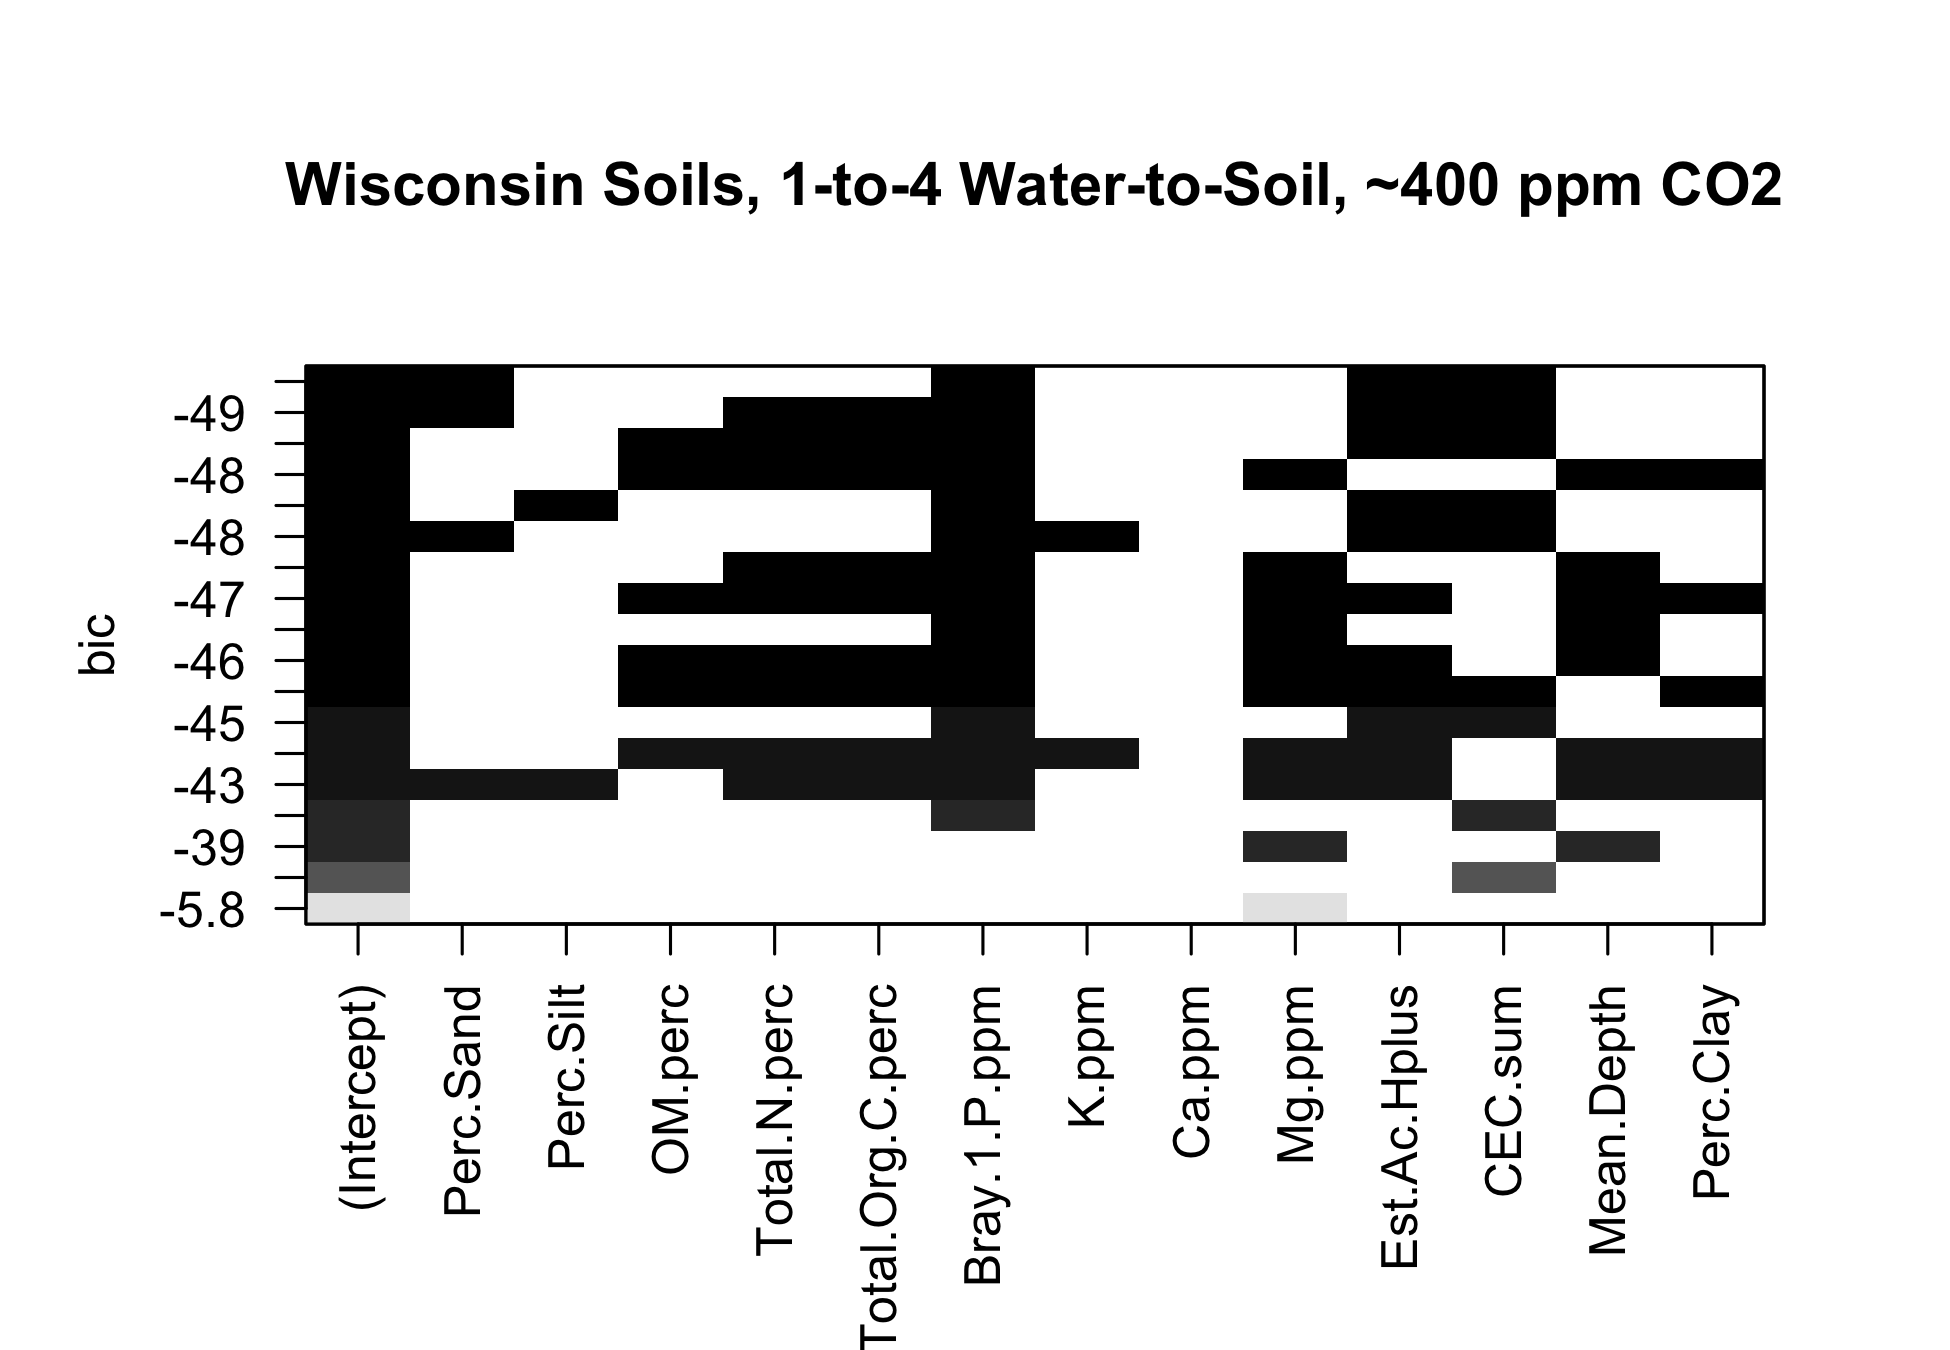
\includegraphics{output-rmd/bic.wisc.one2four.labco2-1.png}

\begin{Shaded}
\begin{Highlighting}[]
\NormalTok{bic.wisc.one2four.highco2 <-}\StringTok{ }\KeywordTok{regsubsets}\NormalTok{(High.CO2.pH }\OperatorTok{~}\StringTok{ }\NormalTok{Perc.Sand }\OperatorTok{+}\StringTok{ }\NormalTok{Perc.Silt }\OperatorTok{+}\StringTok{ }\NormalTok{Perc.Clay }\OperatorTok{+}\StringTok{ }\NormalTok{OM.perc }\OperatorTok{+}\StringTok{ }\NormalTok{Total.N.perc }\OperatorTok{+}\StringTok{ }\NormalTok{Total.Org.C.perc }\OperatorTok{+}\StringTok{ }\NormalTok{Bray.}\FloatTok{1.}\NormalTok{P.ppm }\OperatorTok{+}\StringTok{ }\NormalTok{K.ppm }\OperatorTok{+}\StringTok{ }\NormalTok{Ca.ppm }\OperatorTok{+}\StringTok{ }\NormalTok{Mg.ppm }\OperatorTok{+}\StringTok{ }\NormalTok{Est.Ac.Hplus }\OperatorTok{+}\StringTok{ }\NormalTok{CEC.sum }\OperatorTok{+}\StringTok{ }\NormalTok{Mean.Depth, }\DataTypeTok{nbest =} \DecValTok{2}\NormalTok{,}\DataTypeTok{data =}\NormalTok{ dat.wisc.}\FloatTok{1.}\NormalTok{to}\FloatTok{.4}\NormalTok{)}
\end{Highlighting}
\end{Shaded}

\begin{verbatim}
## Reordering variables and trying again:
\end{verbatim}

\begin{Shaded}
\begin{Highlighting}[]
\KeywordTok{plot}\NormalTok{(bic.wisc.one2four.highco2, }\DataTypeTok{scale=}\StringTok{'bic'}\NormalTok{, }\DataTypeTok{main=}\StringTok{"Wisconsin Soils, 1-to-4 Water-to-Soil, ~2% CO2"}\NormalTok{)}
\end{Highlighting}
\end{Shaded}

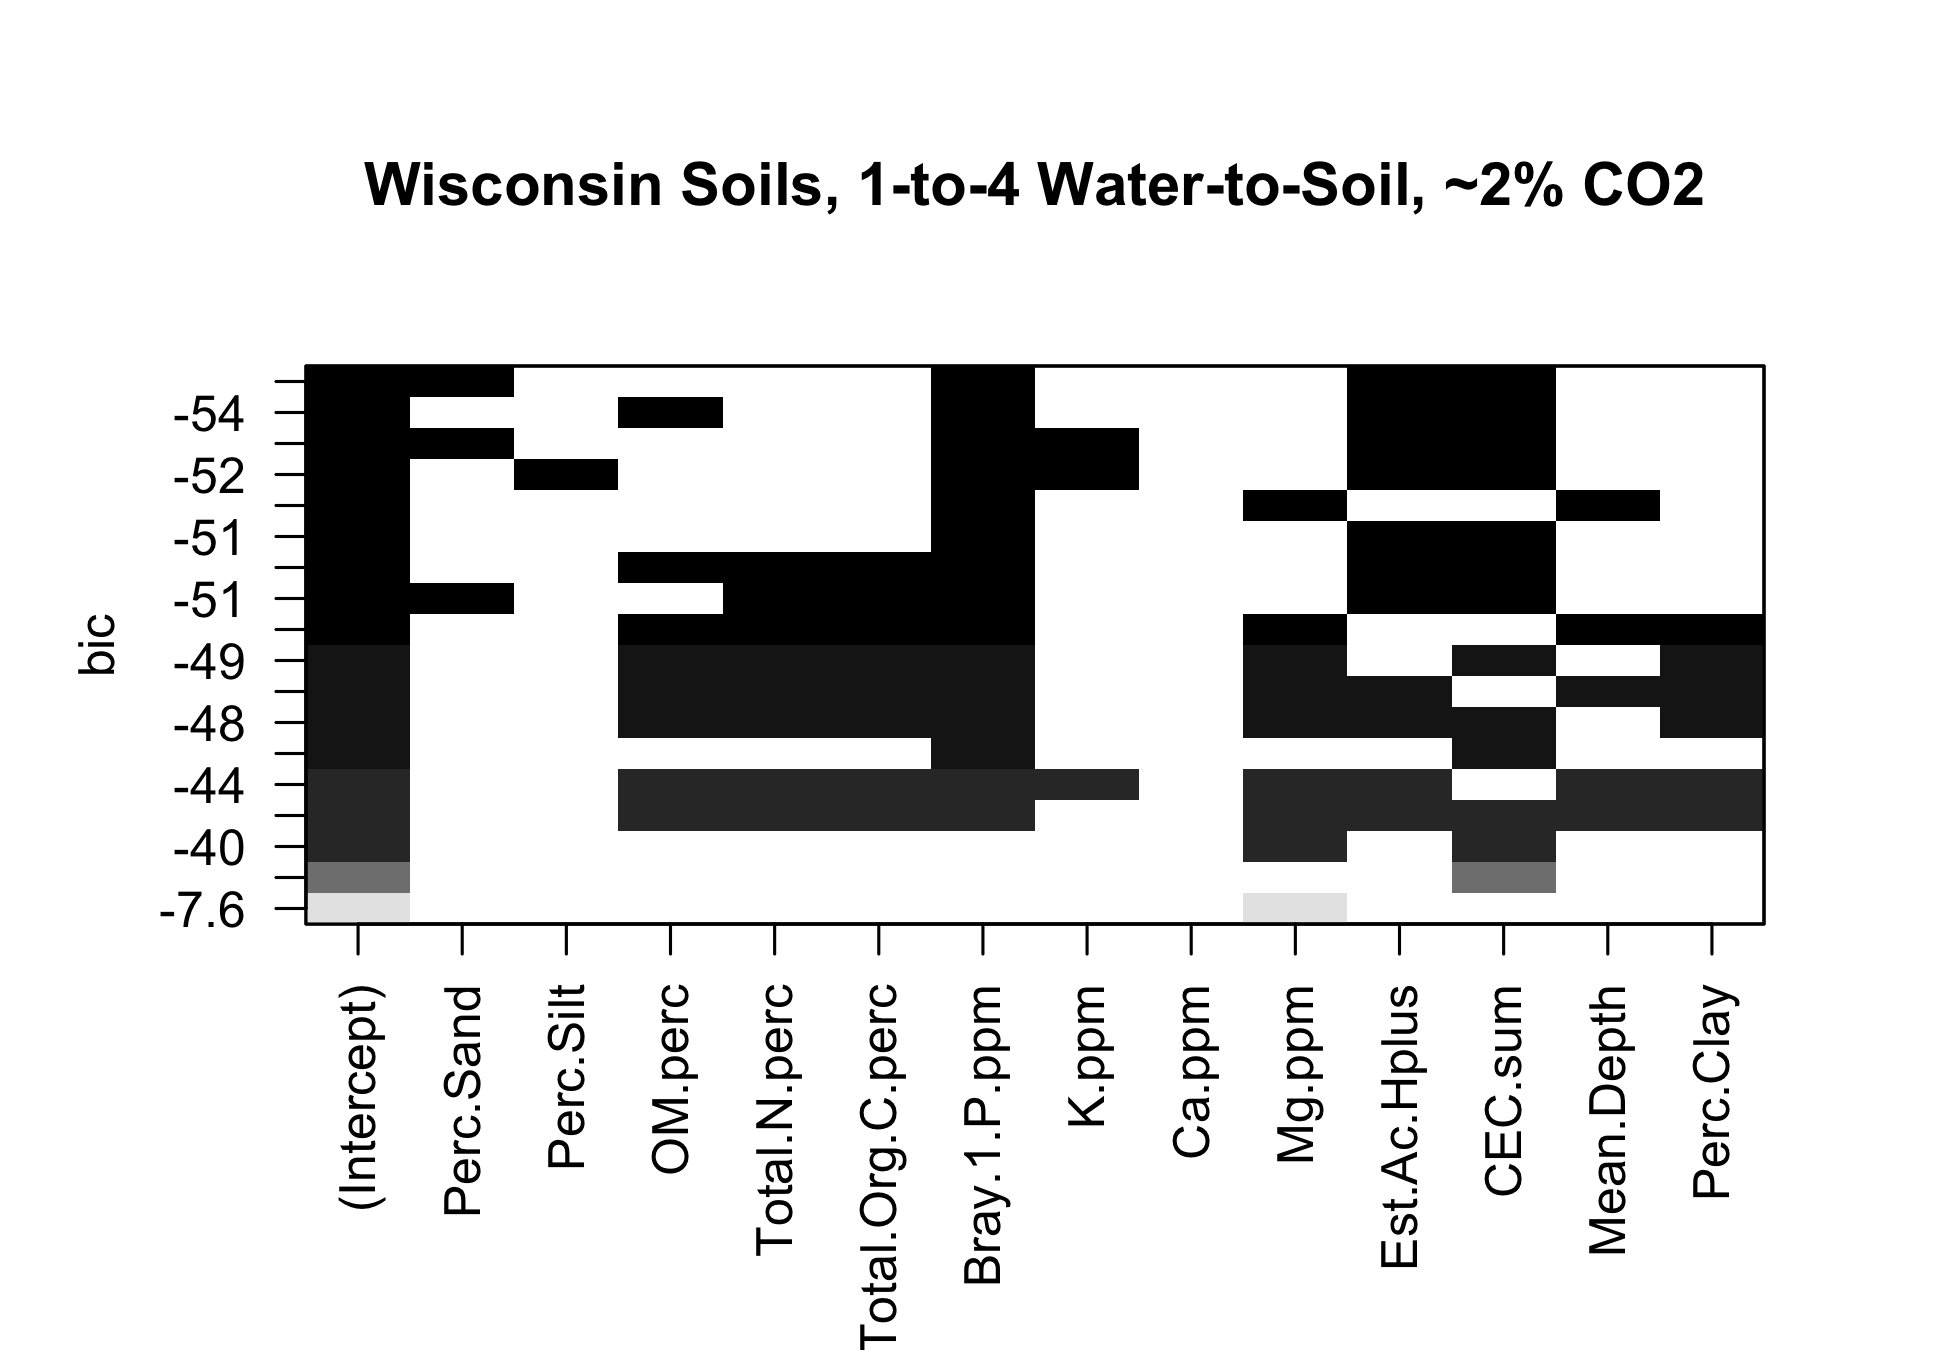
\includegraphics{output-rmd/bic.wisc.one2four.highco2-1.png}

\hypertarget{soil-ph-values}{%
\subsection{Soil pH Values}\label{soil-ph-values}}

\hypertarget{wisconsin}{%
\subsubsection{Wisconsin}\label{wisconsin}}

\begin{Shaded}
\begin{Highlighting}[]
\NormalTok{q1 <-}\StringTok{ }\KeywordTok{qplot}\NormalTok{(}\DataTypeTok{data =}\NormalTok{ dat.wisc, }\DataTypeTok{x =}\NormalTok{ Lab.CO2.pH, }\DataTypeTok{y =}\NormalTok{ High.CO2.pH, }\DataTypeTok{color =}\NormalTok{ Water.Soil.Ratio, }\DataTypeTok{shape =}\NormalTok{ Water.Soil.Ratio) }\OperatorTok{+}\StringTok{ }\KeywordTok{geom_point}\NormalTok{(}\DataTypeTok{size=}\DecValTok{2}\NormalTok{) }\OperatorTok{+}
\StringTok{  }\KeywordTok{theme_bw}\NormalTok{() }\OperatorTok{+}\StringTok{ }\KeywordTok{geom_smooth}\NormalTok{(}\DataTypeTok{method =} \StringTok{"glm"}\NormalTok{) }\OperatorTok{+}\StringTok{ }
\StringTok{  }\KeywordTok{geom_abline}\NormalTok{(}\DataTypeTok{slope =} \DecValTok{1}\NormalTok{, }\DataTypeTok{intercept =} \DecValTok{0}\NormalTok{, }\DataTypeTok{color =} \StringTok{"black"}\NormalTok{) }\OperatorTok{+}\StringTok{ }
\StringTok{  }\KeywordTok{labs}\NormalTok{(}\DataTypeTok{color=}\StringTok{'Solution-to-Soil }\CharTok{\textbackslash{}n}\StringTok{ Ratio by Mass'}\NormalTok{, }
       \DataTypeTok{x =} \StringTok{"pH of Extract at 0.04% carbon dioxide"}\NormalTok{, }
       \DataTypeTok{y =} \StringTok{"pH of Extract at 2.2% carbon dioxide"}\NormalTok{)  }\OperatorTok{+}\StringTok{ }
\StringTok{  }\KeywordTok{ggtitle}\NormalTok{(}\StringTok{"Cross-Wisconsin Soil pH Gradient"}\NormalTok{)}
\NormalTok{q1}
\end{Highlighting}
\end{Shaded}

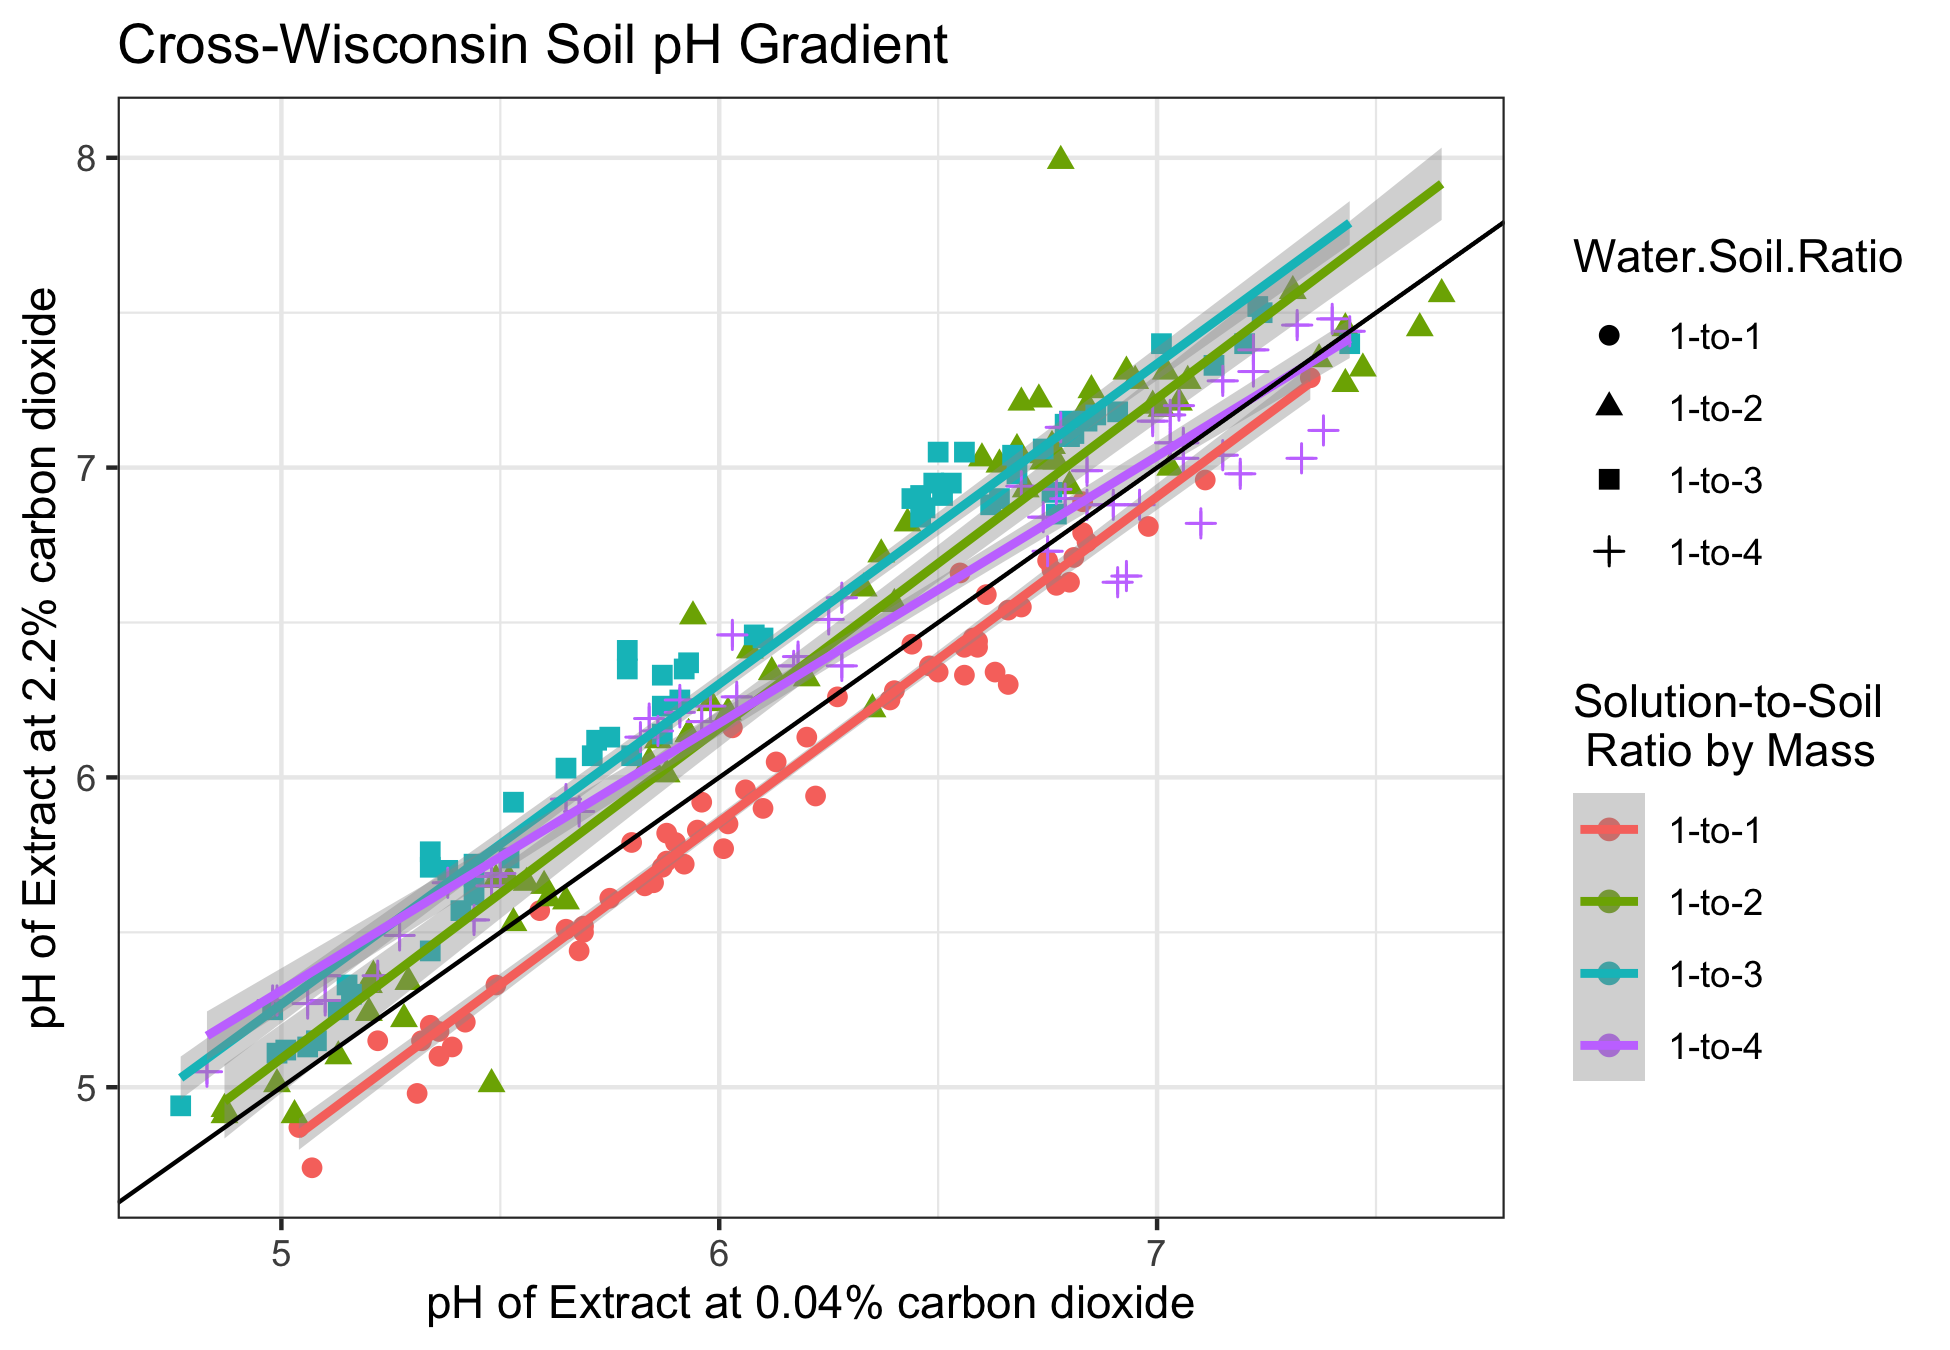
\includegraphics{output-rmd/wisc-stand-sim-soil-ph-1.png}

\begin{Shaded}
\begin{Highlighting}[]
\NormalTok{dat.wisc.one2one <-}\StringTok{ }\KeywordTok{subset}\NormalTok{(dat.wisc, Water.Soil.Ratio}\OperatorTok{==}\StringTok{"1-to-1"}\NormalTok{)}
\NormalTok{lm.dat.wisc.one2one <-}\StringTok{ }\KeywordTok{lm}\NormalTok{(dat.wisc.one2one}\OperatorTok{$}\NormalTok{High.CO2.pH }\OperatorTok{~}\StringTok{ }\NormalTok{dat.wisc.one2one}\OperatorTok{$}\NormalTok{Lab.CO2.pH)}
\KeywordTok{summary}\NormalTok{(lm.dat.wisc.one2one)}
\end{Highlighting}
\end{Shaded}

\begin{verbatim}
## 
## Call:
## lm(formula = dat.wisc.one2one$High.CO2.pH ~ dat.wisc.one2one$Lab.CO2.pH)
## 
## Residuals:
##       Min        1Q    Median        3Q       Max 
## -0.249086 -0.048414 -0.004408  0.039746  0.272258 
## 
## Coefficients:
##                             Estimate Std. Error t value Pr(>|t|)    
## (Intercept)                 -0.44227    0.12905  -3.427   0.0011 ** 
## dat.wisc.one2one$Lab.CO2.pH  1.04975    0.02092  50.169   <2e-16 ***
## ---
## Signif. codes:  0 '***' 0.001 '**' 0.01 '*' 0.05 '.' 0.1 ' ' 1
## 
## Residual standard error: 0.09233 on 61 degrees of freedom
## Multiple R-squared:  0.9763, Adjusted R-squared:  0.9759 
## F-statistic:  2517 on 1 and 61 DF,  p-value: < 2.2e-16
\end{verbatim}

\begin{Shaded}
\begin{Highlighting}[]
\NormalTok{dat.wisc.one2two <-}\StringTok{ }\KeywordTok{subset}\NormalTok{(dat.wisc, Water.Soil.Ratio}\OperatorTok{==}\StringTok{"1-to-2"}\NormalTok{)}
\NormalTok{lm.dat.wisc.one2two <-}\StringTok{ }\KeywordTok{lm}\NormalTok{(dat.wisc.one2two}\OperatorTok{$}\NormalTok{High.CO2.pH }\OperatorTok{~}\StringTok{ }\NormalTok{dat.wisc.one2two}\OperatorTok{$}\NormalTok{Lab.CO2.pH)}
\KeywordTok{summary}\NormalTok{(lm.dat.wisc.one2two)}
\end{Highlighting}
\end{Shaded}

\begin{verbatim}
## 
## Call:
## lm(formula = dat.wisc.one2two$High.CO2.pH ~ dat.wisc.one2two$Lab.CO2.pH)
## 
## Residuals:
##      Min       1Q   Median       3Q      Max 
## -0.59421 -0.07712  0.02317  0.10261  1.00080 
## 
## Coefficients:
##                             Estimate Std. Error t value Pr(>|t|)    
## (Intercept)                 -0.23404    0.24083  -0.972    0.335    
## dat.wisc.one2two$Lab.CO2.pH  1.06537    0.03806  27.995   <2e-16 ***
## ---
## Signif. codes:  0 '***' 0.001 '**' 0.01 '*' 0.05 '.' 0.1 ' ' 1
## 
## Residual standard error: 0.2301 on 61 degrees of freedom
## Multiple R-squared:  0.9278, Adjusted R-squared:  0.9266 
## F-statistic: 783.7 on 1 and 61 DF,  p-value: < 2.2e-16
\end{verbatim}

\begin{Shaded}
\begin{Highlighting}[]
\NormalTok{dat.wisc.one2three <-}\StringTok{ }\KeywordTok{subset}\NormalTok{(dat.wisc, Water.Soil.Ratio}\OperatorTok{==}\StringTok{"1-to-3"}\NormalTok{)}
\NormalTok{lm.dat.wisc.one2three <-}\StringTok{ }\KeywordTok{lm}\NormalTok{(dat.wisc.one2three}\OperatorTok{$}\NormalTok{High.CO2.pH }\OperatorTok{~}\StringTok{ }\NormalTok{dat.wisc.one2three}\OperatorTok{$}\NormalTok{Lab.CO2.pH)}
\KeywordTok{summary}\NormalTok{(lm.dat.wisc.one2three)}
\end{Highlighting}
\end{Shaded}

\begin{verbatim}
## 
## Call:
## lm(formula = dat.wisc.one2three$High.CO2.pH ~ dat.wisc.one2three$Lab.CO2.pH)
## 
## Residuals:
##      Min       1Q   Median       3Q      Max 
## -0.38996 -0.08660 -0.00256  0.08868  0.32564 
## 
## Coefficients:
##                               Estimate Std. Error t value Pr(>|t|)    
## (Intercept)                    0.09923    0.14422   0.688    0.494    
## dat.wisc.one2three$Lab.CO2.pH  1.03370    0.02353  43.937   <2e-16 ***
## ---
## Signif. codes:  0 '***' 0.001 '**' 0.01 '*' 0.05 '.' 0.1 ' ' 1
## 
## Residual standard error: 0.1315 on 61 degrees of freedom
## Multiple R-squared:  0.9694, Adjusted R-squared:  0.9689 
## F-statistic:  1930 on 1 and 61 DF,  p-value: < 2.2e-16
\end{verbatim}

\begin{Shaded}
\begin{Highlighting}[]
\NormalTok{dat.wisc.one2four <-}\StringTok{ }\KeywordTok{subset}\NormalTok{(dat.wisc, Water.Soil.Ratio}\OperatorTok{==}\StringTok{"1-to-4"}\NormalTok{)}
\NormalTok{lm.dat.wisc.one2four <-}\StringTok{ }\KeywordTok{lm}\NormalTok{(dat.wisc.one2four}\OperatorTok{$}\NormalTok{High.CO2.pH }\OperatorTok{~}\StringTok{ }\NormalTok{dat.wisc.one2four}\OperatorTok{$}\NormalTok{Lab.CO2.pH)}
\KeywordTok{summary}\NormalTok{(lm.dat.wisc.one2four)}
\end{Highlighting}
\end{Shaded}

\begin{verbatim}
## 
## Call:
## lm(formula = dat.wisc.one2four$High.CO2.pH ~ dat.wisc.one2four$Lab.CO2.pH)
## 
## Residuals:
##      Min       1Q   Median       3Q      Max 
## -0.32919 -0.07474  0.02195  0.10508  0.28291 
## 
## Coefficients:
##                              Estimate Std. Error t value Pr(>|t|)    
## (Intercept)                   1.00085    0.15157   6.603 1.56e-08 ***
## dat.wisc.one2four$Lab.CO2.pH  0.86228    0.02373  36.334  < 2e-16 ***
## ---
## Signif. codes:  0 '***' 0.001 '**' 0.01 '*' 0.05 '.' 0.1 ' ' 1
## 
## Residual standard error: 0.1402 on 56 degrees of freedom
##   (5 observations deleted due to missingness)
## Multiple R-squared:  0.9593, Adjusted R-squared:  0.9586 
## F-statistic:  1320 on 1 and 56 DF,  p-value: < 2.2e-16
\end{verbatim}

\begin{Shaded}
\begin{Highlighting}[]
\NormalTok{q2 <-}\StringTok{ }\KeywordTok{qplot}\NormalTok{(}\DataTypeTok{data =}\NormalTok{ dat.wisc, }\DataTypeTok{x =} \DecValTok{10}\OperatorTok{^-}\NormalTok{Lab.CO2.pH, }\DataTypeTok{y =} \DecValTok{10}\OperatorTok{^-}\NormalTok{High.CO2.pH, }\DataTypeTok{color =}\NormalTok{ Water.Soil.Ratio, }\DataTypeTok{shape =}\NormalTok{ Water.Soil.Ratio) }\OperatorTok{+}\StringTok{ }\KeywordTok{geom_point}\NormalTok{(}\DataTypeTok{size=}\DecValTok{2}\NormalTok{) }\OperatorTok{+}\StringTok{ }\KeywordTok{scale_x_continuous}\NormalTok{(}\DataTypeTok{limits =} \KeywordTok{c}\NormalTok{(}\DecValTok{10}\OperatorTok{^-}\FloatTok{8.1}\NormalTok{, }\DecValTok{10}\OperatorTok{^-}\FloatTok{4.8}\NormalTok{)) }\OperatorTok{+}\StringTok{ }\KeywordTok{scale_y_continuous}\NormalTok{(}\DataTypeTok{limits =} \KeywordTok{c}\NormalTok{(}\DecValTok{10}\OperatorTok{^-}\FloatTok{8.1}\NormalTok{, }\DecValTok{10}\OperatorTok{^-}\FloatTok{4.8}\NormalTok{)) }\OperatorTok{+}\StringTok{ }\KeywordTok{theme_bw}\NormalTok{() }\OperatorTok{+}\StringTok{ }\KeywordTok{geom_smooth}\NormalTok{(}\DataTypeTok{method =} \StringTok{"glm"}\NormalTok{) }\OperatorTok{+}\StringTok{ }\KeywordTok{geom_abline}\NormalTok{(}\DataTypeTok{slope =} \DecValTok{1}\NormalTok{, }\DataTypeTok{intercept =} \DecValTok{0}\NormalTok{, }\DataTypeTok{color =} \StringTok{"black"}\NormalTok{)}\OperatorTok{+}
\StringTok{  }\KeywordTok{labs}\NormalTok{(}\DataTypeTok{color=}\StringTok{'Solution-to-Soil }\CharTok{\textbackslash{}n}\StringTok{ Ratio by Mass'}\NormalTok{, }
       \DataTypeTok{x =} \StringTok{"a(H+)[M] of Extract at 0.04% carbon dioxide"}\NormalTok{, }
       \DataTypeTok{y =} \StringTok{"a(H+)[M] of Extract at 2.2% carbon dioxide"}\NormalTok{) }\OperatorTok{+}\StringTok{ }
\StringTok{  }\KeywordTok{ggtitle}\NormalTok{(}\StringTok{"Cross-Wisconsin Soil pH Gradient"}\NormalTok{)}
\NormalTok{q2}
\end{Highlighting}
\end{Shaded}

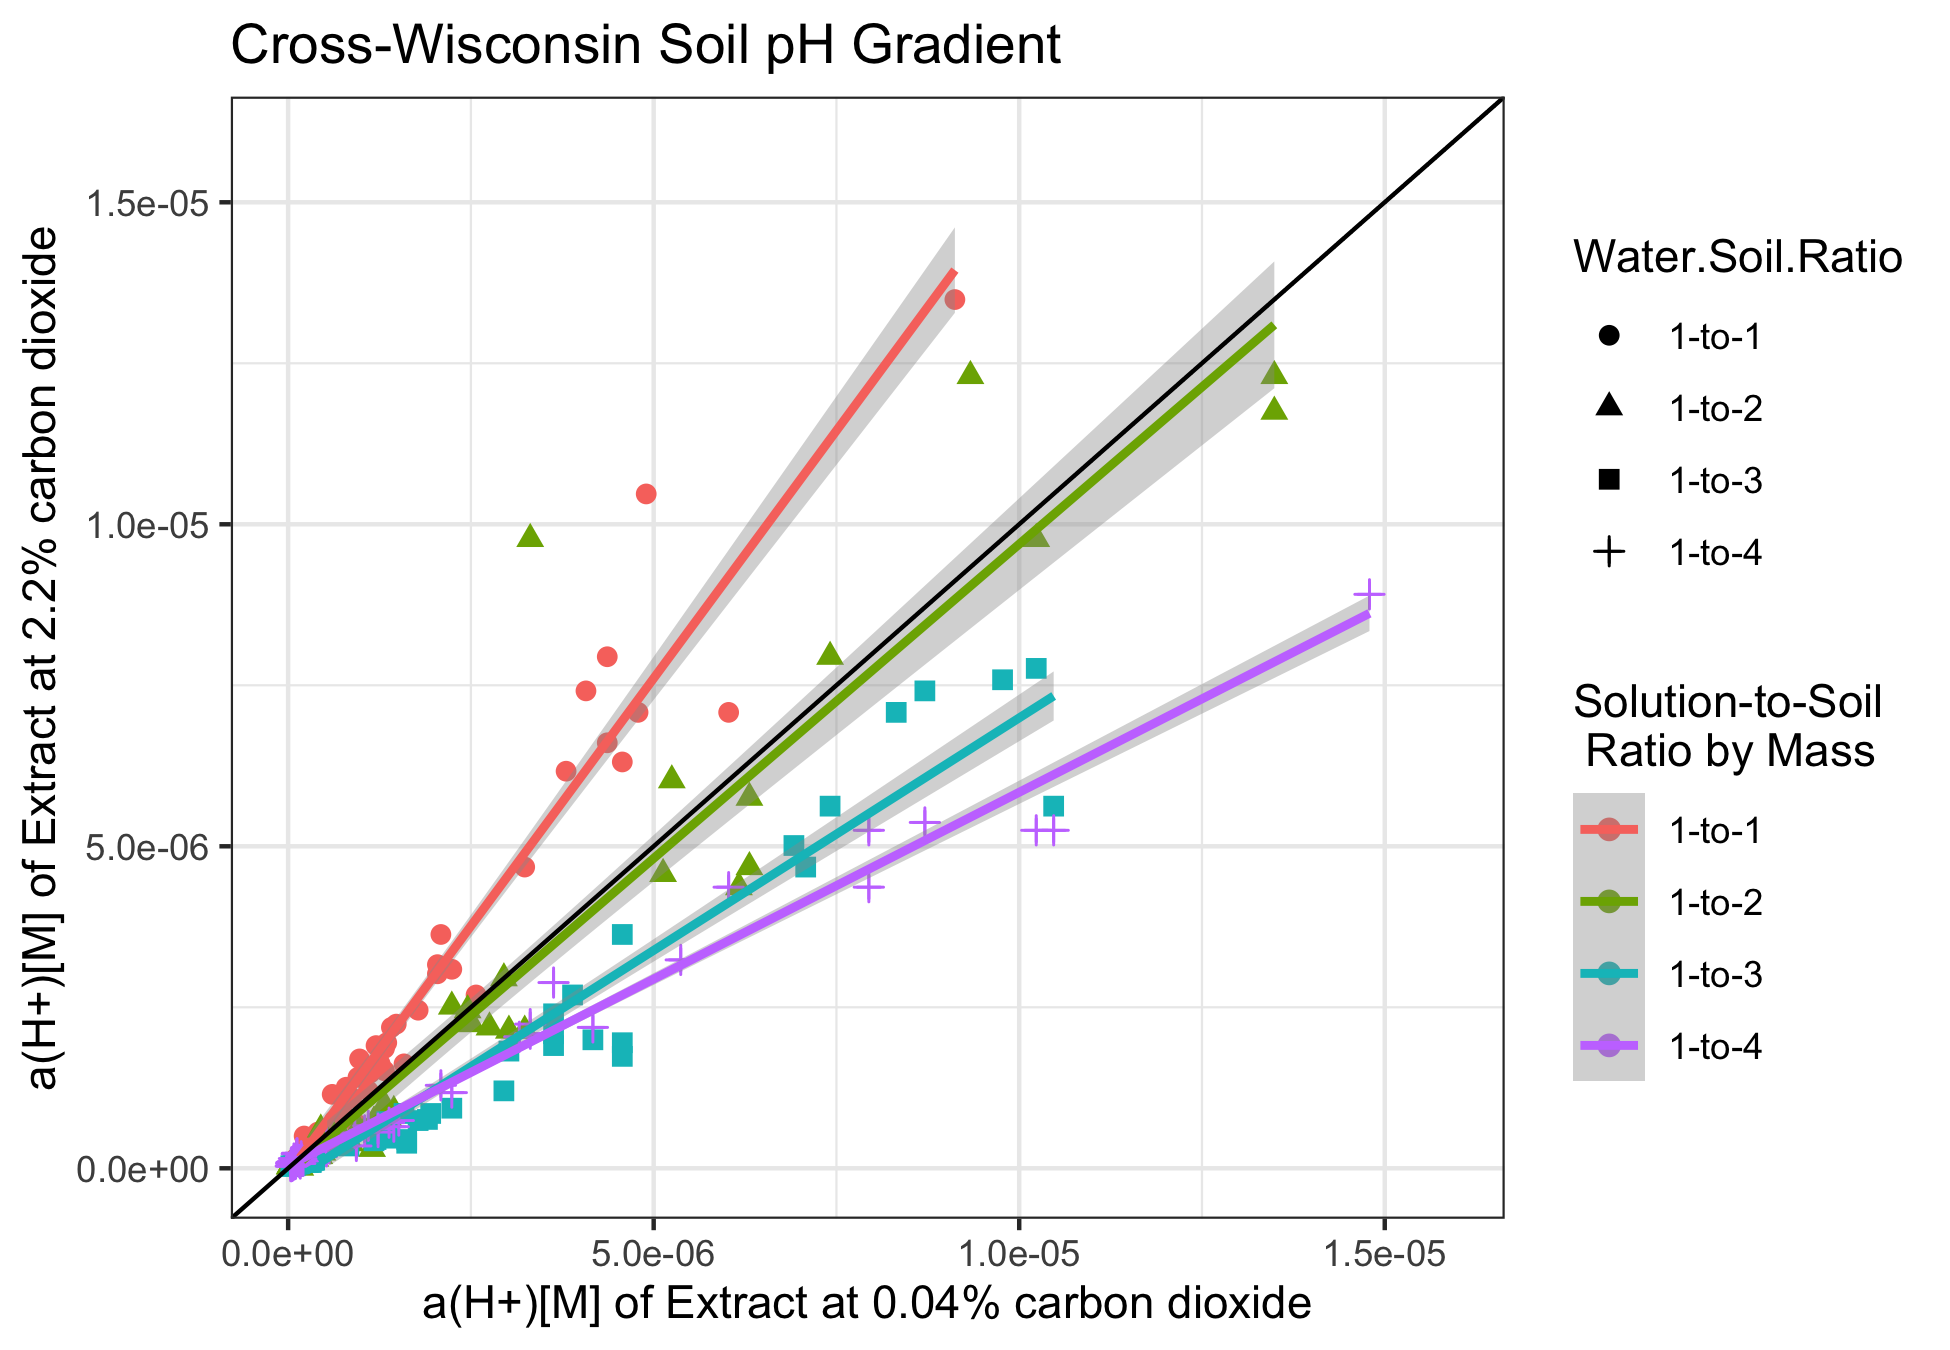
\includegraphics{output-rmd/wisc-stand-sim-soil-hplus-1.png}

\begin{Shaded}
\begin{Highlighting}[]
\NormalTok{dat.wisc}\OperatorTok{$}\NormalTok{Lab.CO2.pH.exp <-}\StringTok{ }\DecValTok{10}\OperatorTok{^-}\NormalTok{dat.wisc}\OperatorTok{$}\NormalTok{Lab.CO2.pH}
\NormalTok{dat.wisc}\OperatorTok{$}\NormalTok{High.CO2.pH.exp <-}\StringTok{ }\DecValTok{10}\OperatorTok{^-}\NormalTok{dat.wisc}\OperatorTok{$}\NormalTok{High.CO2.pH}
\NormalTok{dat.wisc.exp.one2one <-}\StringTok{ }\KeywordTok{subset}\NormalTok{(dat.wisc, Water.Soil.Ratio}\OperatorTok{==}\StringTok{"1-to-1"}\NormalTok{)}
\NormalTok{lm.exp.dat.wisc.exp.one2one <-}\StringTok{ }\KeywordTok{lm}\NormalTok{(dat.wisc.exp.one2one}\OperatorTok{$}\NormalTok{High.CO2.pH.exp }\OperatorTok{~}\StringTok{ }\NormalTok{dat.wisc.exp.one2one}\OperatorTok{$}\NormalTok{Lab.CO2.pH.exp)}
\KeywordTok{summary}\NormalTok{(lm.exp.dat.wisc.exp.one2one)}
\end{Highlighting}
\end{Shaded}

\begin{verbatim}
## 
## Call:
## lm(formula = dat.wisc.exp.one2one$High.CO2.pH.exp ~ dat.wisc.exp.one2one$Lab.CO2.pH.exp)
## 
## Residuals:
##        Min         1Q     Median         3Q        Max 
## -2.857e-06 -1.630e-07  1.056e-07  1.725e-07  4.066e-06 
## 
## Coefficients:
##                                       Estimate Std. Error t value Pr(>|t|)    
## (Intercept)                         -2.306e-07  1.334e-07  -1.729   0.0888 .  
## dat.wisc.exp.one2one$Lab.CO2.pH.exp  1.687e+00  5.350e-02  31.540   <2e-16 ***
## ---
## Signif. codes:  0 '***' 0.001 '**' 0.01 '*' 0.05 '.' 0.1 ' ' 1
## 
## Residual standard error: 8.34e-07 on 61 degrees of freedom
## Multiple R-squared:  0.9422, Adjusted R-squared:  0.9413 
## F-statistic: 994.8 on 1 and 61 DF,  p-value: < 2.2e-16
\end{verbatim}

\begin{Shaded}
\begin{Highlighting}[]
\NormalTok{dat.wisc.exp.one2two <-}\StringTok{ }\KeywordTok{subset}\NormalTok{(dat.wisc, Water.Soil.Ratio}\OperatorTok{==}\StringTok{"1-to-2"}\NormalTok{)}
\NormalTok{lm.exp.dat.wisc.exp.one2two <-}\StringTok{ }\KeywordTok{lm}\NormalTok{(dat.wisc.exp.one2two}\OperatorTok{$}\NormalTok{High.CO2.pH.exp }\OperatorTok{~}\StringTok{ }\NormalTok{dat.wisc.exp.one2two}\OperatorTok{$}\NormalTok{Lab.CO2.pH.exp)}
\KeywordTok{summary}\NormalTok{(lm.exp.dat.wisc.exp.one2two)}
\end{Highlighting}
\end{Shaded}

\begin{verbatim}
## 
## Call:
## lm(formula = dat.wisc.exp.one2two$High.CO2.pH.exp ~ dat.wisc.exp.one2two$Lab.CO2.pH.exp)
## 
## Residuals:
##        Min         1Q     Median         3Q        Max 
## -1.586e-06 -2.932e-07 -4.740e-08  4.260e-08  6.607e-06 
## 
## Coefficients:
##                                       Estimate Std. Error t value Pr(>|t|)    
## (Intercept)                         -6.567e-08  1.555e-07  -0.422    0.674    
## dat.wisc.exp.one2two$Lab.CO2.pH.exp  9.758e-01  4.204e-02  23.209   <2e-16 ***
## ---
## Signif. codes:  0 '***' 0.001 '**' 0.01 '*' 0.05 '.' 0.1 ' ' 1
## 
## Residual standard error: 1.047e-06 on 61 degrees of freedom
## Multiple R-squared:  0.8983, Adjusted R-squared:  0.8966 
## F-statistic: 538.7 on 1 and 61 DF,  p-value: < 2.2e-16
\end{verbatim}

\begin{Shaded}
\begin{Highlighting}[]
\NormalTok{dat.wisc.exp.one2three <-}\StringTok{ }\KeywordTok{subset}\NormalTok{(dat.wisc, Water.Soil.Ratio}\OperatorTok{==}\StringTok{"1-to-3"}\NormalTok{)}
\NormalTok{lm.exp.dat.wisc.exp.one2three <-}\StringTok{ }\KeywordTok{lm}\NormalTok{(dat.wisc.exp.one2three}\OperatorTok{$}\NormalTok{High.CO2.pH.exp }\OperatorTok{~}\StringTok{ }\NormalTok{dat.wisc.exp.one2three}\OperatorTok{$}\NormalTok{Lab.CO2.pH.exp)}
\KeywordTok{summary}\NormalTok{(lm.exp.dat.wisc.exp.one2three)}
\end{Highlighting}
\end{Shaded}

\begin{verbatim}
## 
## Call:
## lm(formula = dat.wisc.exp.one2three$High.CO2.pH.exp ~ dat.wisc.exp.one2three$Lab.CO2.pH.exp)
## 
## Residuals:
##        Min         1Q     Median         3Q        Max 
## -1.611e-06 -2.007e-07  1.015e-07  1.774e-07  1.430e-06 
## 
## Coefficients:
##                                         Estimate Std. Error t value Pr(>|t|)
## (Intercept)                           -2.074e-07  7.690e-08  -2.697  0.00903
## dat.wisc.exp.one2three$Lab.CO2.pH.exp  7.107e-01  1.853e-02  38.349  < 2e-16
##                                          
## (Intercept)                           ** 
## dat.wisc.exp.one2three$Lab.CO2.pH.exp ***
## ---
## Signif. codes:  0 '***' 0.001 '**' 0.01 '*' 0.05 '.' 0.1 ' ' 1
## 
## Residual standard error: 4.962e-07 on 61 degrees of freedom
## Multiple R-squared:  0.9602, Adjusted R-squared:  0.9595 
## F-statistic:  1471 on 1 and 61 DF,  p-value: < 2.2e-16
\end{verbatim}

\begin{Shaded}
\begin{Highlighting}[]
\NormalTok{dat.wisc.exp.one2four <-}\StringTok{ }\KeywordTok{subset}\NormalTok{(dat.wisc, Water.Soil.Ratio}\OperatorTok{==}\StringTok{"1-to-4"}\NormalTok{)}
\NormalTok{lm.exp.dat.wisc.exp.one2four <-}\StringTok{ }\KeywordTok{lm}\NormalTok{(dat.wisc.exp.one2four}\OperatorTok{$}\NormalTok{High.CO2.pH.exp }\OperatorTok{~}\StringTok{ }\NormalTok{dat.wisc.exp.one2four}\OperatorTok{$}\NormalTok{Lab.CO2.pH.exp)}
\KeywordTok{summary}\NormalTok{(lm.exp.dat.wisc.exp.one2four)}
\end{Highlighting}
\end{Shaded}

\begin{verbatim}
## 
## Call:
## lm(formula = dat.wisc.exp.one2four$High.CO2.pH.exp ~ dat.wisc.exp.one2four$Lab.CO2.pH.exp)
## 
## Residuals:
##        Min         1Q     Median         3Q        Max 
## -8.640e-07 -5.226e-08 -1.407e-08  3.586e-08  8.317e-07 
## 
## Coefficients:
##                                       Estimate Std. Error t value Pr(>|t|)    
## (Intercept)                          3.850e-08  3.903e-08   0.987    0.328    
## dat.wisc.exp.one2four$Lab.CO2.pH.exp 5.800e-01  1.059e-02  54.768   <2e-16 ***
## ---
## Signif. codes:  0 '***' 0.001 '**' 0.01 '*' 0.05 '.' 0.1 ' ' 1
## 
## Residual standard error: 2.547e-07 on 56 degrees of freedom
##   (5 observations deleted due to missingness)
## Multiple R-squared:  0.9817, Adjusted R-squared:  0.9813 
## F-statistic:  3000 on 1 and 56 DF,  p-value: < 2.2e-16
\end{verbatim}

\hypertarget{spooner}{%
\subsubsection{Spooner}\label{spooner}}

\begin{Shaded}
\begin{Highlighting}[]
\NormalTok{dat.spooner <-}\StringTok{ }\KeywordTok{subset}\NormalTok{(dat, Study}\OperatorTok{==}\StringTok{"Spooner"}\NormalTok{)}
\end{Highlighting}
\end{Shaded}

\begin{Shaded}
\begin{Highlighting}[]
\NormalTok{q3 <-}\StringTok{ }\KeywordTok{qplot}\NormalTok{(}\DataTypeTok{data =}\NormalTok{ dat.spooner, }\DataTypeTok{x =}\NormalTok{ Lab.CO2.pH, }\DataTypeTok{y =}\NormalTok{ High.CO2.pH, }\DataTypeTok{color =}\NormalTok{ Water.Soil.Ratio, }\DataTypeTok{shape =}\NormalTok{ Water.Soil.Ratio) }\OperatorTok{+}\StringTok{ }\KeywordTok{geom_point}\NormalTok{(}\DataTypeTok{size=}\DecValTok{2}\NormalTok{) }\OperatorTok{+}
\StringTok{  }\KeywordTok{theme_bw}\NormalTok{() }\OperatorTok{+}\StringTok{ }\KeywordTok{geom_smooth}\NormalTok{(}\DataTypeTok{method =} \StringTok{"glm"}\NormalTok{) }\OperatorTok{+}\StringTok{ }
\StringTok{  }\KeywordTok{geom_abline}\NormalTok{(}\DataTypeTok{slope =} \DecValTok{1}\NormalTok{, }\DataTypeTok{intercept =} \DecValTok{0}\NormalTok{, }\DataTypeTok{color =} \StringTok{"black"}\NormalTok{) }\OperatorTok{+}\StringTok{ }
\StringTok{  }\KeywordTok{labs}\NormalTok{(}\DataTypeTok{color=}\StringTok{'Solution-to-Soil }\CharTok{\textbackslash{}n}\StringTok{ Ratio by Mass'}\NormalTok{, }
       \DataTypeTok{x =} \StringTok{"pH of Extract at 0.04% carbon dioxide"}\NormalTok{, }
       \DataTypeTok{y =} \StringTok{"pH of Extract at 2.2% carbon dioxide"}\NormalTok{)  }\OperatorTok{+}\StringTok{ }
\StringTok{  }\KeywordTok{ggtitle}\NormalTok{(}\StringTok{"Long-term Soil pH Manipulation"}\NormalTok{)}
\NormalTok{q3}
\end{Highlighting}
\end{Shaded}

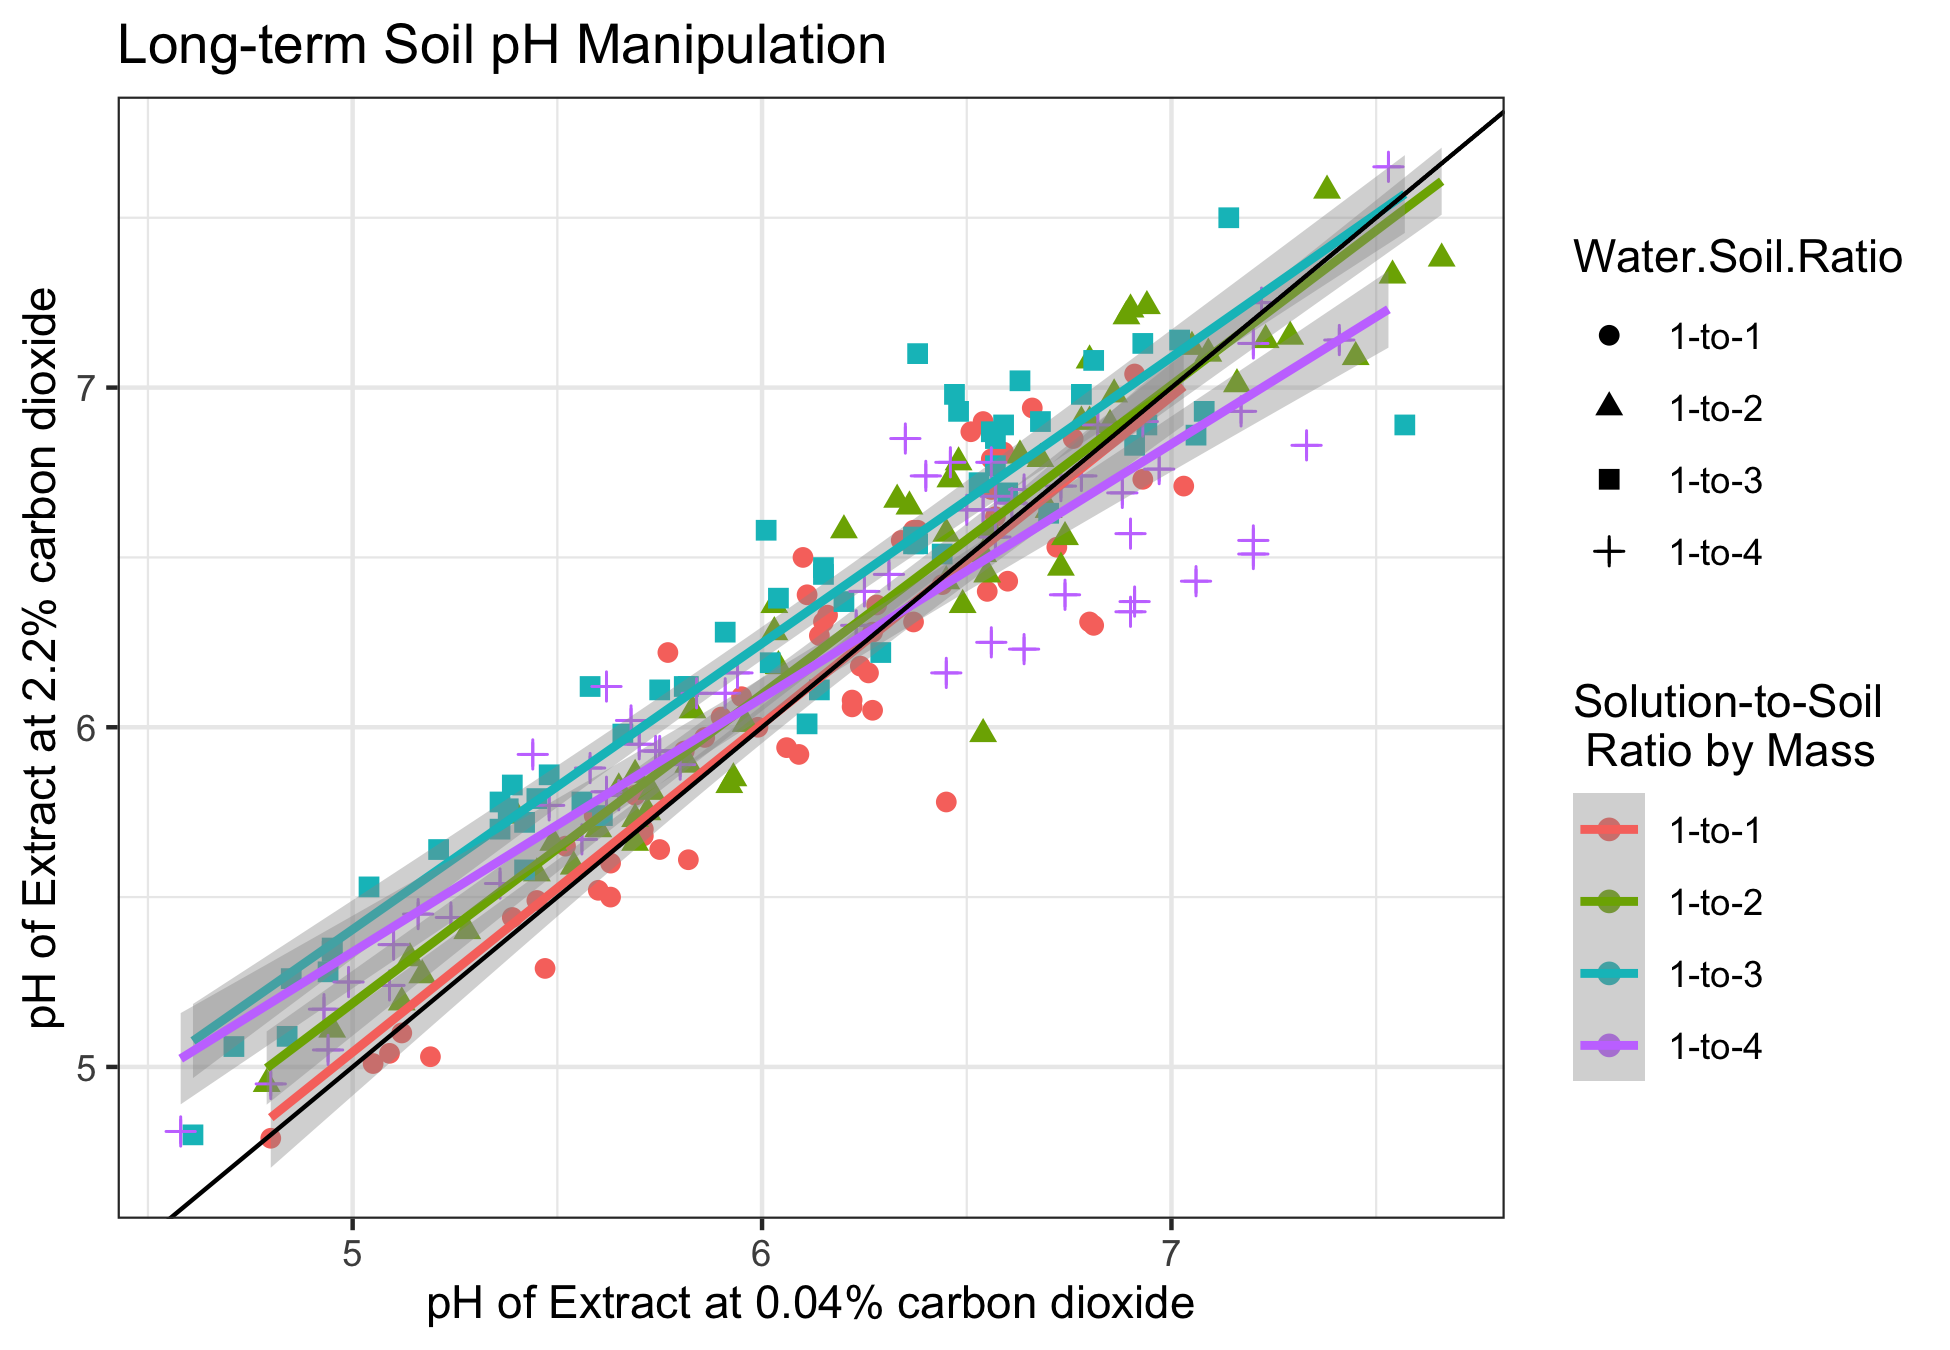
\includegraphics{output-rmd/spooner-stand-sim-soil-ph-1.png}

\begin{Shaded}
\begin{Highlighting}[]
\NormalTok{dat.spooner.one2one <-}\StringTok{ }\KeywordTok{subset}\NormalTok{(dat.spooner, Water.Soil.Ratio}\OperatorTok{==}\StringTok{"1-to-1"}\NormalTok{)}
\NormalTok{lm.dat.spooner.one2one <-}\StringTok{ }\KeywordTok{lm}\NormalTok{(dat.spooner.one2one}\OperatorTok{$}\NormalTok{High.CO2.pH }\OperatorTok{~}\StringTok{ }\NormalTok{dat.spooner.one2one}\OperatorTok{$}\NormalTok{Lab.CO2.pH)}
\KeywordTok{summary}\NormalTok{(lm.dat.spooner.one2one)}
\end{Highlighting}
\end{Shaded}

\begin{verbatim}
## 
## Call:
## lm(formula = dat.spooner.one2one$High.CO2.pH ~ dat.spooner.one2one$Lab.CO2.pH)
## 
## Residuals:
##      Min       1Q   Median       3Q      Max 
## -0.66320 -0.14009 -0.00638  0.13470  0.43313 
## 
## Coefficients:
##                                Estimate Std. Error t value Pr(>|t|)    
## (Intercept)                     0.21771    0.33090   0.658    0.513    
## dat.spooner.one2one$Lab.CO2.pH  0.96519    0.05413  17.832   <2e-16 ***
## ---
## Signif. codes:  0 '***' 0.001 '**' 0.01 '*' 0.05 '.' 0.1 ' ' 1
## 
## Residual standard error: 0.2161 on 58 degrees of freedom
## Multiple R-squared:  0.8457, Adjusted R-squared:  0.8431 
## F-statistic:   318 on 1 and 58 DF,  p-value: < 2.2e-16
\end{verbatim}

\begin{Shaded}
\begin{Highlighting}[]
\NormalTok{dat.spooner.one2two <-}\StringTok{ }\KeywordTok{subset}\NormalTok{(dat.spooner, Water.Soil.Ratio}\OperatorTok{==}\StringTok{"1-to-2"}\NormalTok{)}
\NormalTok{lm.dat.spooner.one2two <-}\StringTok{ }\KeywordTok{lm}\NormalTok{(dat.spooner.one2two}\OperatorTok{$}\NormalTok{High.CO2.pH }\OperatorTok{~}\StringTok{ }\NormalTok{dat.spooner.one2two}\OperatorTok{$}\NormalTok{Lab.CO2.pH)}
\KeywordTok{summary}\NormalTok{(lm.dat.spooner.one2two)}
\end{Highlighting}
\end{Shaded}

\begin{verbatim}
## 
## Call:
## lm(formula = dat.spooner.one2two$High.CO2.pH ~ dat.spooner.one2two$Lab.CO2.pH)
## 
## Residuals:
##      Min       1Q   Median       3Q      Max 
## -0.60874 -0.09311 -0.02963  0.10190  0.31373 
## 
## Coefficients:
##                                Estimate Std. Error t value Pr(>|t|)    
## (Intercept)                      0.6387     0.2092   3.052  0.00342 ** 
## dat.spooner.one2two$Lab.CO2.pH   0.9098     0.0330  27.570  < 2e-16 ***
## ---
## Signif. codes:  0 '***' 0.001 '**' 0.01 '*' 0.05 '.' 0.1 ' ' 1
## 
## Residual standard error: 0.1788 on 58 degrees of freedom
## Multiple R-squared:  0.9291, Adjusted R-squared:  0.9279 
## F-statistic: 760.1 on 1 and 58 DF,  p-value: < 2.2e-16
\end{verbatim}

\begin{Shaded}
\begin{Highlighting}[]
\NormalTok{dat.spooner.one2three <-}\StringTok{ }\KeywordTok{subset}\NormalTok{(dat.spooner, Water.Soil.Ratio}\OperatorTok{==}\StringTok{"1-to-3"}\NormalTok{)}
\NormalTok{lm.dat.spooner.one2three <-}\StringTok{ }\KeywordTok{lm}\NormalTok{(dat.spooner.one2three}\OperatorTok{$}\NormalTok{High.CO2.pH }\OperatorTok{~}\StringTok{ }\NormalTok{dat.spooner.one2three}\OperatorTok{$}\NormalTok{Lab.CO2.pH)}
\KeywordTok{summary}\NormalTok{(lm.dat.spooner.one2three)}
\end{Highlighting}
\end{Shaded}

\begin{verbatim}
## 
## Call:
## lm(formula = dat.spooner.one2three$High.CO2.pH ~ dat.spooner.one2three$Lab.CO2.pH)
## 
## Residuals:
##      Min       1Q   Median       3Q      Max 
## -0.67980 -0.09748  0.02187  0.09653  0.53270 
## 
## Coefficients:
##                                  Estimate Std. Error t value Pr(>|t|)    
## (Intercept)                       1.19251    0.21155   5.637 5.36e-07 ***
## dat.spooner.one2three$Lab.CO2.pH  0.84244    0.03475  24.240  < 2e-16 ***
## ---
## Signif. codes:  0 '***' 0.001 '**' 0.01 '*' 0.05 '.' 0.1 ' ' 1
## 
## Residual standard error: 0.1912 on 58 degrees of freedom
## Multiple R-squared:  0.9102, Adjusted R-squared:  0.9086 
## F-statistic: 587.6 on 1 and 58 DF,  p-value: < 2.2e-16
\end{verbatim}

\begin{Shaded}
\begin{Highlighting}[]
\NormalTok{dat.spooner.one2four <-}\StringTok{ }\KeywordTok{subset}\NormalTok{(dat.spooner, Water.Soil.Ratio}\OperatorTok{==}\StringTok{"1-to-4"}\NormalTok{)}
\NormalTok{lm.dat.spooner.one2four <-}\StringTok{ }\KeywordTok{lm}\NormalTok{(dat.spooner.one2four}\OperatorTok{$}\NormalTok{High.CO2.pH }\OperatorTok{~}\StringTok{ }\NormalTok{dat.spooner.one2four}\OperatorTok{$}\NormalTok{Lab.CO2.pH)}
\KeywordTok{summary}\NormalTok{(lm.dat.spooner.one2four)}
\end{Highlighting}
\end{Shaded}

\begin{verbatim}
## 
## Call:
## lm(formula = dat.spooner.one2four$High.CO2.pH ~ dat.spooner.one2four$Lab.CO2.pH)
## 
## Residuals:
##     Min      1Q  Median      3Q     Max 
## -0.4737 -0.1284  0.0345  0.1339  0.5020 
## 
## Coefficients:
##                                 Estimate Std. Error t value Pr(>|t|)    
## (Intercept)                      1.59886    0.23789   6.721 8.61e-09 ***
## dat.spooner.one2four$Lab.CO2.pH  0.74789    0.03798  19.691  < 2e-16 ***
## ---
## Signif. codes:  0 '***' 0.001 '**' 0.01 '*' 0.05 '.' 0.1 ' ' 1
## 
## Residual standard error: 0.2238 on 58 degrees of freedom
## Multiple R-squared:  0.8699, Adjusted R-squared:  0.8676 
## F-statistic: 387.7 on 1 and 58 DF,  p-value: < 2.2e-16
\end{verbatim}

\begin{Shaded}
\begin{Highlighting}[]
\NormalTok{q4 <-}\StringTok{ }\KeywordTok{qplot}\NormalTok{(}\DataTypeTok{data =}\NormalTok{ dat.spooner, }\DataTypeTok{x =} \DecValTok{10}\OperatorTok{^-}\NormalTok{Lab.CO2.pH, }\DataTypeTok{y =} \DecValTok{10}\OperatorTok{^-}\NormalTok{High.CO2.pH, }\DataTypeTok{color =}\NormalTok{ Water.Soil.Ratio, }\DataTypeTok{shape =}\NormalTok{ Water.Soil.Ratio) }\OperatorTok{+}\StringTok{ }\KeywordTok{geom_point}\NormalTok{(}\DataTypeTok{size=}\DecValTok{2}\NormalTok{) }\OperatorTok{+}\StringTok{ }\KeywordTok{scale_x_continuous}\NormalTok{(}\DataTypeTok{limits =} \KeywordTok{c}\NormalTok{(}\DecValTok{10}\OperatorTok{^-}\FloatTok{8.1}\NormalTok{, }\DecValTok{10}\OperatorTok{^-}\FloatTok{4.8}\NormalTok{)) }\OperatorTok{+}\StringTok{ }\KeywordTok{scale_y_continuous}\NormalTok{(}\DataTypeTok{limits =} \KeywordTok{c}\NormalTok{(}\DecValTok{10}\OperatorTok{^-}\FloatTok{8.1}\NormalTok{, }\DecValTok{10}\OperatorTok{^-}\FloatTok{4.8}\NormalTok{)) }\OperatorTok{+}\StringTok{ }\KeywordTok{theme_bw}\NormalTok{() }\OperatorTok{+}\StringTok{ }\KeywordTok{geom_smooth}\NormalTok{(}\DataTypeTok{method =} \StringTok{"glm"}\NormalTok{) }\OperatorTok{+}\StringTok{ }\KeywordTok{geom_abline}\NormalTok{(}\DataTypeTok{slope =} \DecValTok{1}\NormalTok{, }\DataTypeTok{intercept =} \DecValTok{0}\NormalTok{, }\DataTypeTok{color =} \StringTok{"black"}\NormalTok{)}\OperatorTok{+}
\StringTok{  }\KeywordTok{labs}\NormalTok{(}\DataTypeTok{color=}\StringTok{'Solution-to-Soil }\CharTok{\textbackslash{}n}\StringTok{ Ratio by Mass'}\NormalTok{, }
       \DataTypeTok{x =} \StringTok{"a(H+)[M] of Extract at 0.04% carbon dioxide"}\NormalTok{, }
       \DataTypeTok{y =} \StringTok{"a(H+)[M] of Extract at 2.2% carbon dioxide"}\NormalTok{) }\OperatorTok{+}\StringTok{ }
\StringTok{  }\KeywordTok{ggtitle}\NormalTok{(}\StringTok{"Long-term Soil pH Manipulation"}\NormalTok{)}
\NormalTok{q4}
\end{Highlighting}
\end{Shaded}

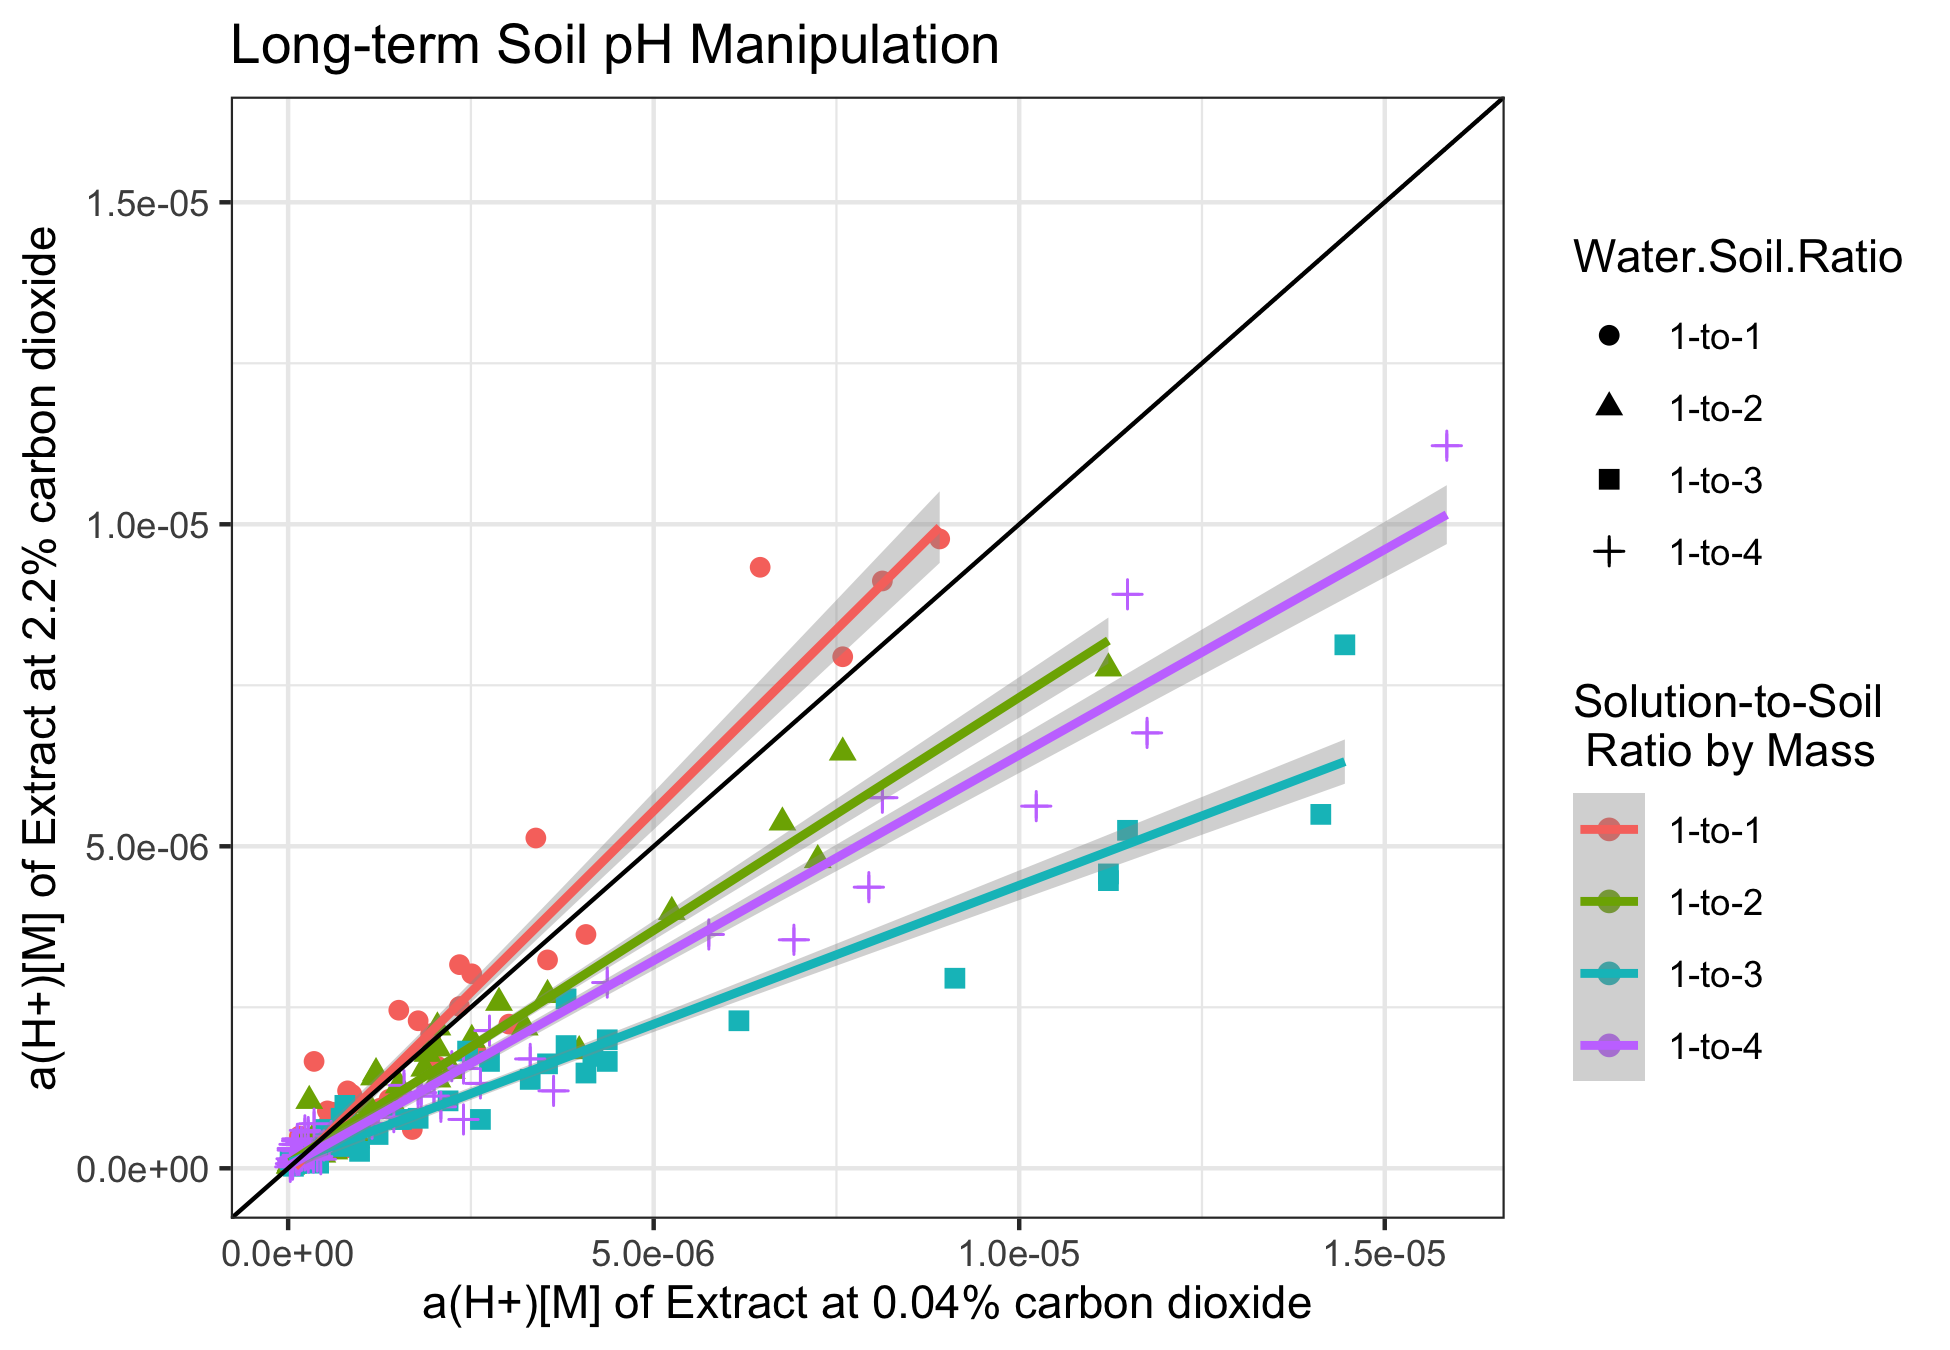
\includegraphics{output-rmd/spooner-stand-sim-soil-hplus-1.png}

\begin{Shaded}
\begin{Highlighting}[]
\NormalTok{dat.spooner}\OperatorTok{$}\NormalTok{Lab.CO2.pH.exp <-}\StringTok{ }\DecValTok{10}\OperatorTok{^-}\NormalTok{dat.spooner}\OperatorTok{$}\NormalTok{Lab.CO2.pH}
\NormalTok{dat.spooner}\OperatorTok{$}\NormalTok{High.CO2.pH.exp <-}\StringTok{ }\DecValTok{10}\OperatorTok{^-}\NormalTok{dat.spooner}\OperatorTok{$}\NormalTok{High.CO2.pH}
\NormalTok{dat.spooner.exp.one2one <-}\StringTok{ }\KeywordTok{subset}\NormalTok{(dat.spooner, Water.Soil.Ratio}\OperatorTok{==}\StringTok{"1-to-1"}\NormalTok{)}
\NormalTok{lm.exp.dat.spooner.exp.one2one <-}\StringTok{ }\KeywordTok{lm}\NormalTok{(dat.spooner.exp.one2one}\OperatorTok{$}\NormalTok{High.CO2.pH.exp }\OperatorTok{~}\StringTok{ }\NormalTok{dat.spooner.exp.one2one}\OperatorTok{$}\NormalTok{Lab.CO2.pH.exp)}
\KeywordTok{summary}\NormalTok{(lm.exp.dat.spooner.exp.one2one)}
\end{Highlighting}
\end{Shaded}

\begin{verbatim}
## 
## Call:
## lm(formula = dat.spooner.exp.one2one$High.CO2.pH.exp ~ dat.spooner.exp.one2one$Lab.CO2.pH.exp)
## 
## Residuals:
##        Min         1Q     Median         3Q        Max 
## -1.204e-06 -2.295e-07 -3.125e-08  2.051e-07  2.410e-06 
## 
## Coefficients:
##                                          Estimate Std. Error t value Pr(>|t|)
## (Intercept)                            -1.981e-08  8.732e-08  -0.227    0.821
## dat.spooner.exp.one2one$Lab.CO2.pH.exp  1.075e+00  2.747e-02  39.136   <2e-16
##                                           
## (Intercept)                               
## dat.spooner.exp.one2one$Lab.CO2.pH.exp ***
## ---
## Signif. codes:  0 '***' 0.001 '**' 0.01 '*' 0.05 '.' 0.1 ' ' 1
## 
## Residual standard error: 5.688e-07 on 58 degrees of freedom
## Multiple R-squared:  0.9635, Adjusted R-squared:  0.9629 
## F-statistic:  1532 on 1 and 58 DF,  p-value: < 2.2e-16
\end{verbatim}

\begin{Shaded}
\begin{Highlighting}[]
\NormalTok{dat.spooner.exp.one2two <-}\StringTok{ }\KeywordTok{subset}\NormalTok{(dat.spooner, Water.Soil.Ratio}\OperatorTok{==}\StringTok{"1-to-2"}\NormalTok{)}
\NormalTok{lm.exp.dat.spooner.exp.one2two <-}\StringTok{ }\KeywordTok{lm}\NormalTok{(dat.spooner.exp.one2two}\OperatorTok{$}\NormalTok{High.CO2.pH.exp }\OperatorTok{~}\StringTok{ }\NormalTok{dat.spooner.exp.one2two}\OperatorTok{$}\NormalTok{Lab.CO2.pH.exp)}
\KeywordTok{summary}\NormalTok{(lm.exp.dat.spooner.exp.one2two)}
\end{Highlighting}
\end{Shaded}

\begin{verbatim}
## 
## Call:
## lm(formula = dat.spooner.exp.one2two$High.CO2.pH.exp ~ dat.spooner.exp.one2two$Lab.CO2.pH.exp)
## 
## Residuals:
##        Min         1Q     Median         3Q        Max 
## -1.086e-06 -1.310e-07 -6.742e-08  1.101e-07  1.004e-06 
## 
## Coefficients:
##                                         Estimate Std. Error t value Pr(>|t|)
## (Intercept)                            9.373e-08  4.586e-08   2.044   0.0455
## dat.spooner.exp.one2two$Lab.CO2.pH.exp 7.065e-01  1.379e-02  51.234   <2e-16
##                                           
## (Intercept)                            *  
## dat.spooner.exp.one2two$Lab.CO2.pH.exp ***
## ---
## Signif. codes:  0 '***' 0.001 '**' 0.01 '*' 0.05 '.' 0.1 ' ' 1
## 
## Residual standard error: 3.085e-07 on 58 degrees of freedom
## Multiple R-squared:  0.9784, Adjusted R-squared:  0.978 
## F-statistic:  2625 on 1 and 58 DF,  p-value: < 2.2e-16
\end{verbatim}

\begin{Shaded}
\begin{Highlighting}[]
\NormalTok{dat.spooner.exp.one2three <-}\StringTok{ }\KeywordTok{subset}\NormalTok{(dat.spooner, Water.Soil.Ratio}\OperatorTok{==}\StringTok{"1-to-3"}\NormalTok{)}
\NormalTok{lm.exp.dat.spooner.exp.one2three <-}\StringTok{ }\KeywordTok{lm}\NormalTok{(dat.spooner.exp.one2three}\OperatorTok{$}\NormalTok{High.CO2.pH.exp }\OperatorTok{~}\StringTok{ }\NormalTok{dat.spooner.exp.one2three}\OperatorTok{$}\NormalTok{Lab.CO2.pH.exp)}
\KeywordTok{summary}\NormalTok{(lm.exp.dat.spooner.exp.one2three)}
\end{Highlighting}
\end{Shaded}

\begin{verbatim}
## 
## Call:
## lm(formula = dat.spooner.exp.one2three$High.CO2.pH.exp ~ dat.spooner.exp.one2three$Lab.CO2.pH.exp)
## 
## Residuals:
##        Min         1Q     Median         3Q        Max 
## -1.618e-06 -8.430e-08  5.650e-08  1.385e-07  3.451e-06 
## 
## Coefficients:
##                                            Estimate Std. Error t value Pr(>|t|)
## (Intercept)                              -5.952e-08  1.007e-07  -0.591    0.557
## dat.spooner.exp.one2three$Lab.CO2.pH.exp  5.075e-01  1.717e-02  29.552   <2e-16
##                                             
## (Intercept)                                 
## dat.spooner.exp.one2three$Lab.CO2.pH.exp ***
## ---
## Signif. codes:  0 '***' 0.001 '**' 0.01 '*' 0.05 '.' 0.1 ' ' 1
## 
## Residual standard error: 6.67e-07 on 58 degrees of freedom
## Multiple R-squared:  0.9377, Adjusted R-squared:  0.9366 
## F-statistic: 873.3 on 1 and 58 DF,  p-value: < 2.2e-16
\end{verbatim}

\begin{Shaded}
\begin{Highlighting}[]
\NormalTok{dat.spooner.exp.one2four <-}\StringTok{ }\KeywordTok{subset}\NormalTok{(dat.spooner, Water.Soil.Ratio}\OperatorTok{==}\StringTok{"1-to-4"}\NormalTok{)}
\NormalTok{lm.exp.dat.spooner.exp.one2four <-}\StringTok{ }\KeywordTok{lm}\NormalTok{(dat.spooner.exp.one2four}\OperatorTok{$}\NormalTok{High.CO2.pH.exp }\OperatorTok{~}\StringTok{ }\NormalTok{dat.spooner.exp.one2four}\OperatorTok{$}\NormalTok{Lab.CO2.pH.exp)}
\KeywordTok{summary}\NormalTok{(lm.exp.dat.spooner.exp.one2four)}
\end{Highlighting}
\end{Shaded}

\begin{verbatim}
## 
## Call:
## lm(formula = dat.spooner.exp.one2four$High.CO2.pH.exp ~ dat.spooner.exp.one2four$Lab.CO2.pH.exp)
## 
## Residuals:
##        Min         1Q     Median         3Q        Max 
## -1.097e-06 -9.412e-08 -1.423e-08  1.356e-07  1.800e-06 
## 
## Coefficients:
##                                          Estimate Std. Error t value Pr(>|t|)
## (Intercept)                             7.342e-08  6.522e-08   1.126    0.265
## dat.spooner.exp.one2four$Lab.CO2.pH.exp 6.131e-01  1.253e-02  48.946   <2e-16
##                                            
## (Intercept)                                
## dat.spooner.exp.one2four$Lab.CO2.pH.exp ***
## ---
## Signif. codes:  0 '***' 0.001 '**' 0.01 '*' 0.05 '.' 0.1 ' ' 1
## 
## Residual standard error: 4.443e-07 on 58 degrees of freedom
## Multiple R-squared:  0.9764, Adjusted R-squared:  0.976 
## F-statistic:  2396 on 1 and 58 DF,  p-value: < 2.2e-16
\end{verbatim}

\hypertarget{grid-of-multifactorial-plots}{%
\subsubsection{Grid of Multifactorial
Plots}\label{grid-of-multifactorial-plots}}

\begin{Shaded}
\begin{Highlighting}[]
\KeywordTok{plot_grid}\NormalTok{(q3, q4, q1, q2) }
\end{Highlighting}
\end{Shaded}

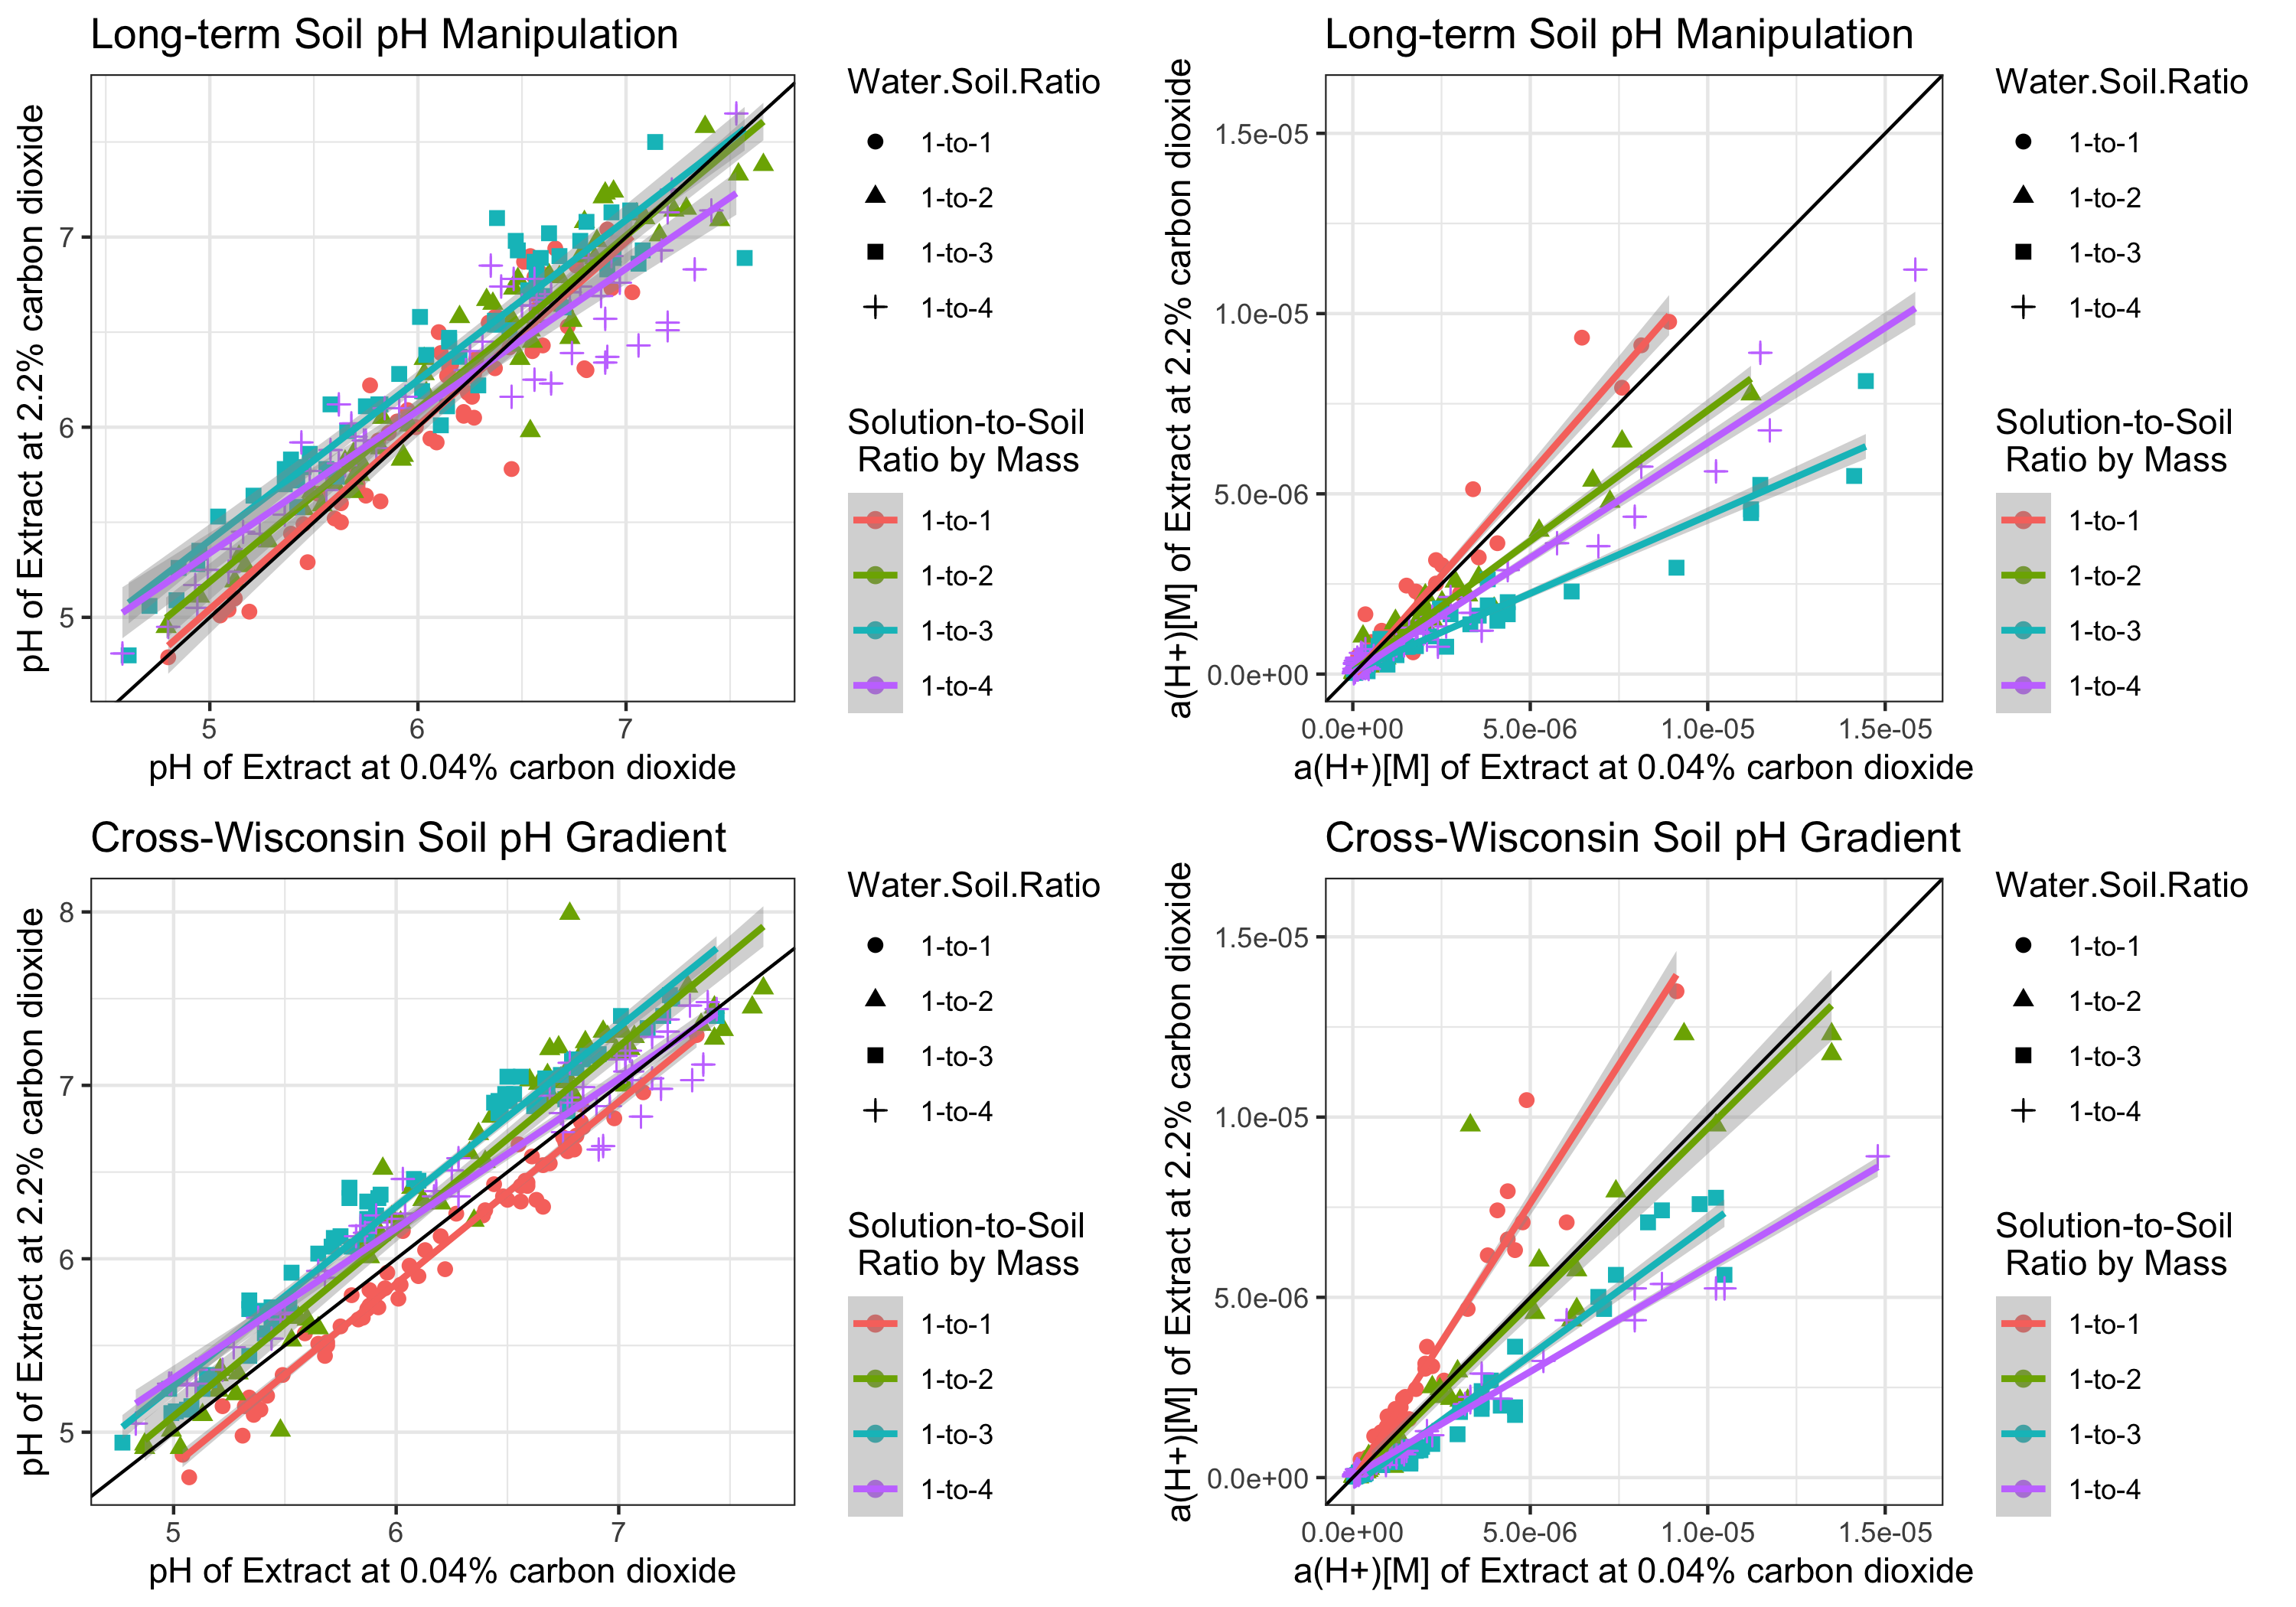
\includegraphics{output-rmd/multifactoral-grid-ph-1.png}

\emph{BLACK AND WHITE}

\begin{Shaded}
\begin{Highlighting}[]
\NormalTok{q1.bw <-}\StringTok{ }\KeywordTok{qplot}\NormalTok{(}\DataTypeTok{data =}\NormalTok{ dat.wisc, }\DataTypeTok{x =}\NormalTok{ Lab.CO2.pH, }\DataTypeTok{y =}\NormalTok{ High.CO2.pH, }\DataTypeTok{shape =}\NormalTok{ Water.Soil.Ratio) }\OperatorTok{+}\StringTok{ }\KeywordTok{geom_point}\NormalTok{(}\DataTypeTok{size=}\DecValTok{2}\NormalTok{) }\OperatorTok{+}
\StringTok{  }\KeywordTok{theme_bw}\NormalTok{() }\OperatorTok{+}\StringTok{ }\KeywordTok{geom_smooth}\NormalTok{(}\DataTypeTok{method =} \StringTok{"glm"}\NormalTok{) }\OperatorTok{+}\StringTok{ }
\StringTok{  }\KeywordTok{geom_abline}\NormalTok{(}\DataTypeTok{slope =} \DecValTok{1}\NormalTok{, }\DataTypeTok{intercept =} \DecValTok{0}\NormalTok{, }\DataTypeTok{color =} \StringTok{"black"}\NormalTok{) }\OperatorTok{+}\StringTok{ }
\StringTok{  }\KeywordTok{labs}\NormalTok{(}\DataTypeTok{color=}\StringTok{'Solution-to-Soil }\CharTok{\textbackslash{}n}\StringTok{ Ratio by Mass'}\NormalTok{, }
       \DataTypeTok{x =} \StringTok{"pH of Extract at 0.04% carbon dioxide"}\NormalTok{, }
       \DataTypeTok{y =} \StringTok{"pH of Extract at 2% carbon dioxide"}\NormalTok{)  }\OperatorTok{+}\StringTok{ }
\StringTok{  }\KeywordTok{ggtitle}\NormalTok{(}\StringTok{"Cross-Wisconsin Soil pH Gradient"}\NormalTok{)}
\NormalTok{q1.bw}
\end{Highlighting}
\end{Shaded}

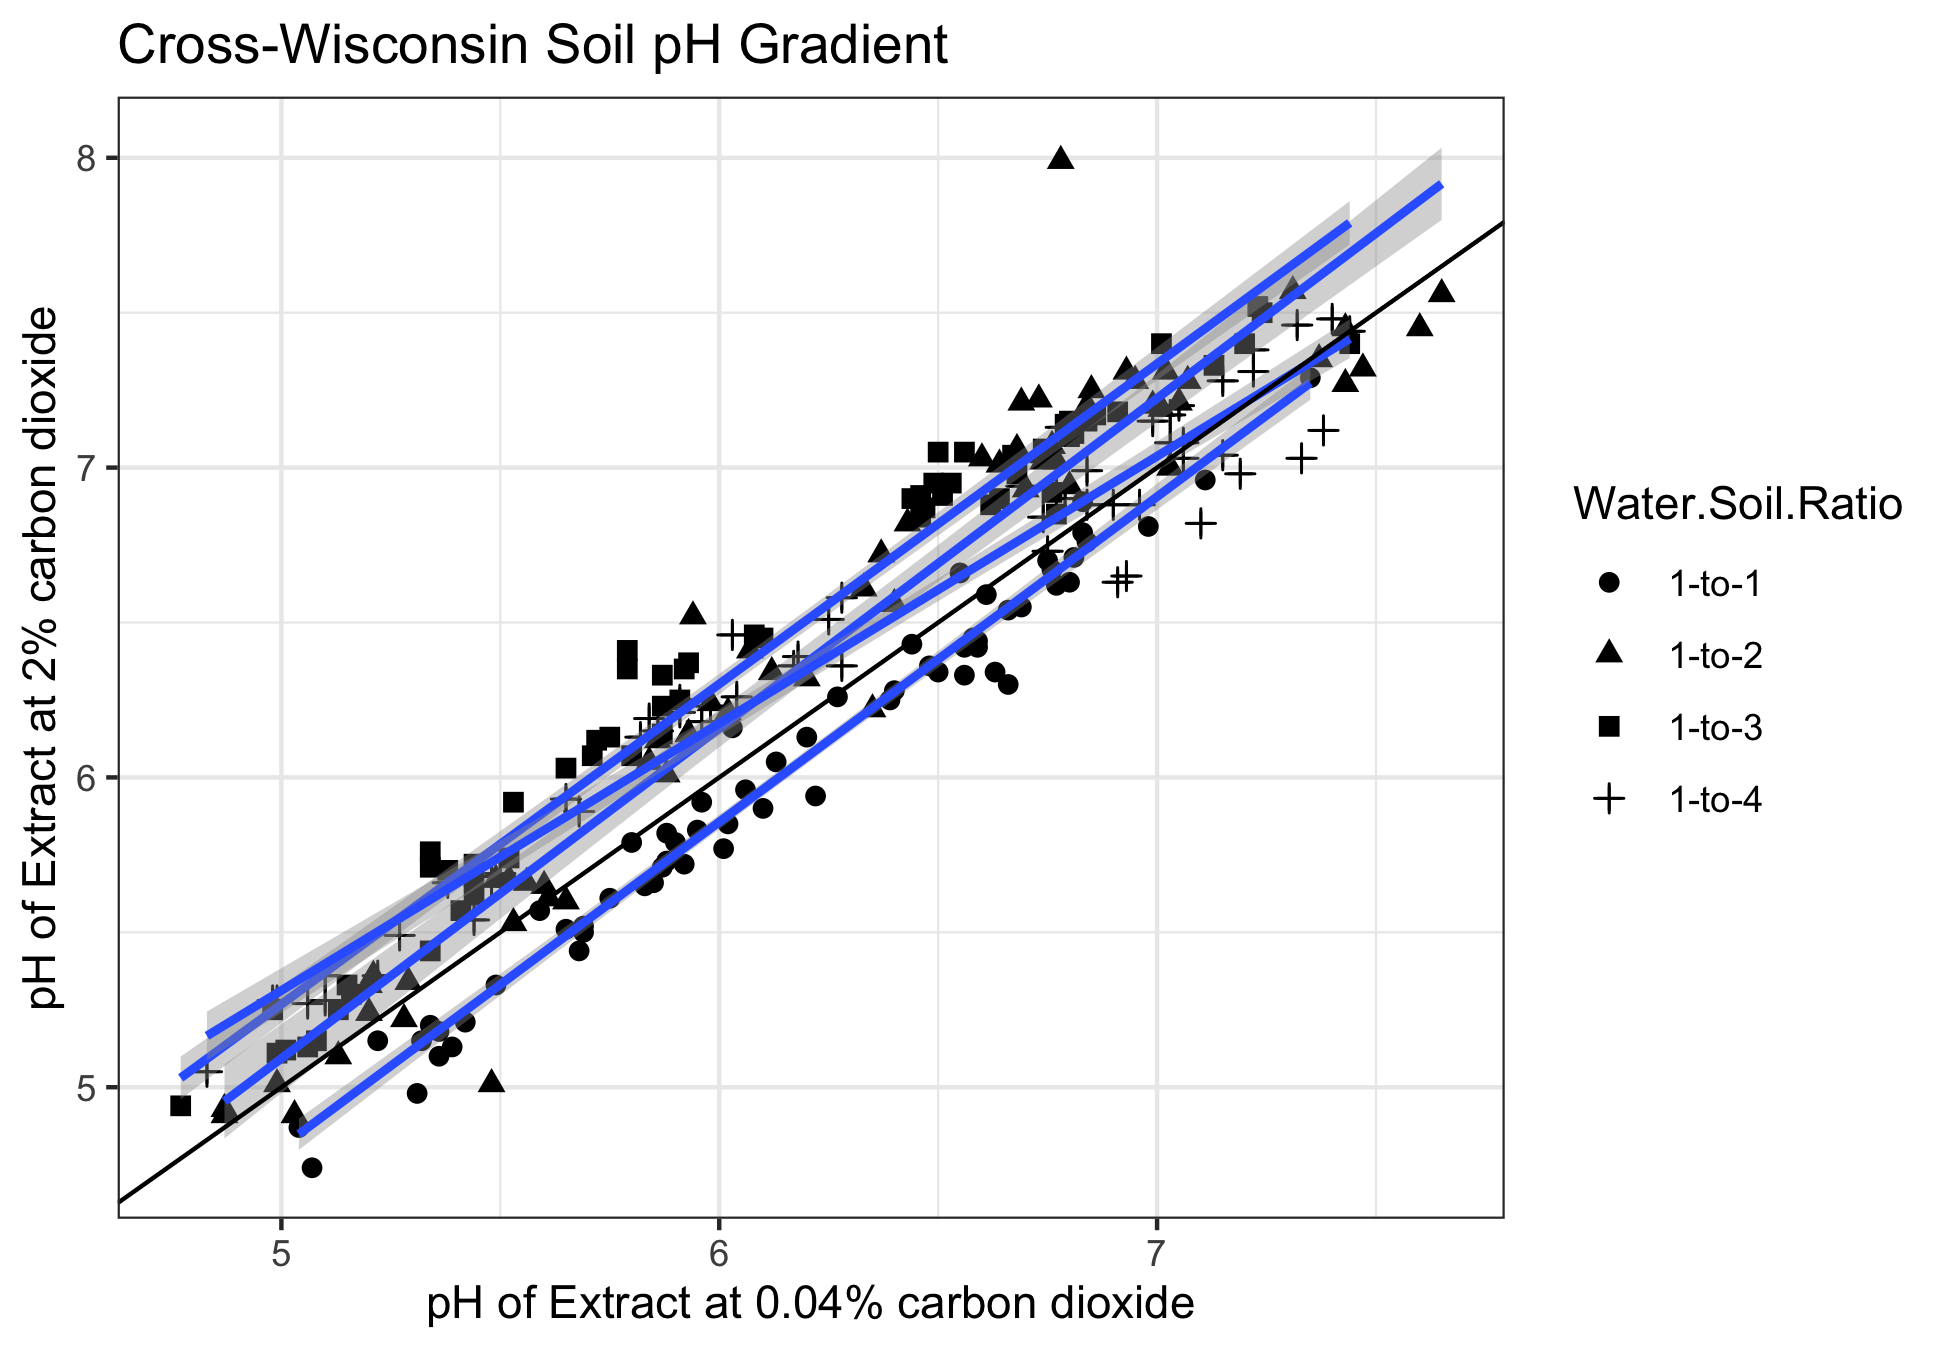
\includegraphics{output-rmd/wisc-stand-sim-soil-ph-bw-1.png}

\begin{Shaded}
\begin{Highlighting}[]
\NormalTok{q2.bw <-}\StringTok{ }\KeywordTok{qplot}\NormalTok{(}\DataTypeTok{data =}\NormalTok{ dat.wisc, }\DataTypeTok{x =} \DecValTok{10}\OperatorTok{^-}\NormalTok{Lab.CO2.pH, }\DataTypeTok{y =} \DecValTok{10}\OperatorTok{^-}\NormalTok{High.CO2.pH, }\DataTypeTok{shape =}\NormalTok{ Water.Soil.Ratio) }\OperatorTok{+}\StringTok{ }\KeywordTok{geom_point}\NormalTok{(}\DataTypeTok{size=}\DecValTok{2}\NormalTok{) }\OperatorTok{+}\StringTok{ }\KeywordTok{scale_x_continuous}\NormalTok{(}\DataTypeTok{limits =} \KeywordTok{c}\NormalTok{(}\DecValTok{10}\OperatorTok{^-}\FloatTok{8.1}\NormalTok{, }\DecValTok{10}\OperatorTok{^-}\FloatTok{4.8}\NormalTok{)) }\OperatorTok{+}\StringTok{ }\KeywordTok{scale_y_continuous}\NormalTok{(}\DataTypeTok{limits =} \KeywordTok{c}\NormalTok{(}\DecValTok{10}\OperatorTok{^-}\FloatTok{8.1}\NormalTok{, }\DecValTok{10}\OperatorTok{^-}\FloatTok{4.8}\NormalTok{)) }\OperatorTok{+}\StringTok{ }\KeywordTok{theme_bw}\NormalTok{() }\OperatorTok{+}\StringTok{ }\KeywordTok{geom_smooth}\NormalTok{(}\DataTypeTok{method =} \StringTok{"glm"}\NormalTok{) }\OperatorTok{+}\StringTok{ }\KeywordTok{geom_abline}\NormalTok{(}\DataTypeTok{slope =} \DecValTok{1}\NormalTok{, }\DataTypeTok{intercept =} \DecValTok{0}\NormalTok{, }\DataTypeTok{color =} \StringTok{"black"}\NormalTok{)}\OperatorTok{+}
\StringTok{  }\KeywordTok{labs}\NormalTok{(}\DataTypeTok{color=}\StringTok{'Solution-to-Soil }\CharTok{\textbackslash{}n}\StringTok{ Ratio by Mass'}\NormalTok{, }
       \DataTypeTok{x =} \StringTok{"a(H+)[M] of Extract at 0.04% carbon dioxide"}\NormalTok{, }
       \DataTypeTok{y =} \StringTok{"a(H+)[M] of Extract at 2% carbon dioxide"}\NormalTok{) }\OperatorTok{+}\StringTok{ }
\StringTok{  }\KeywordTok{ggtitle}\NormalTok{(}\StringTok{"Cross-Wisconsin Soil pH Gradient"}\NormalTok{)}
\NormalTok{q2.bw}
\end{Highlighting}
\end{Shaded}

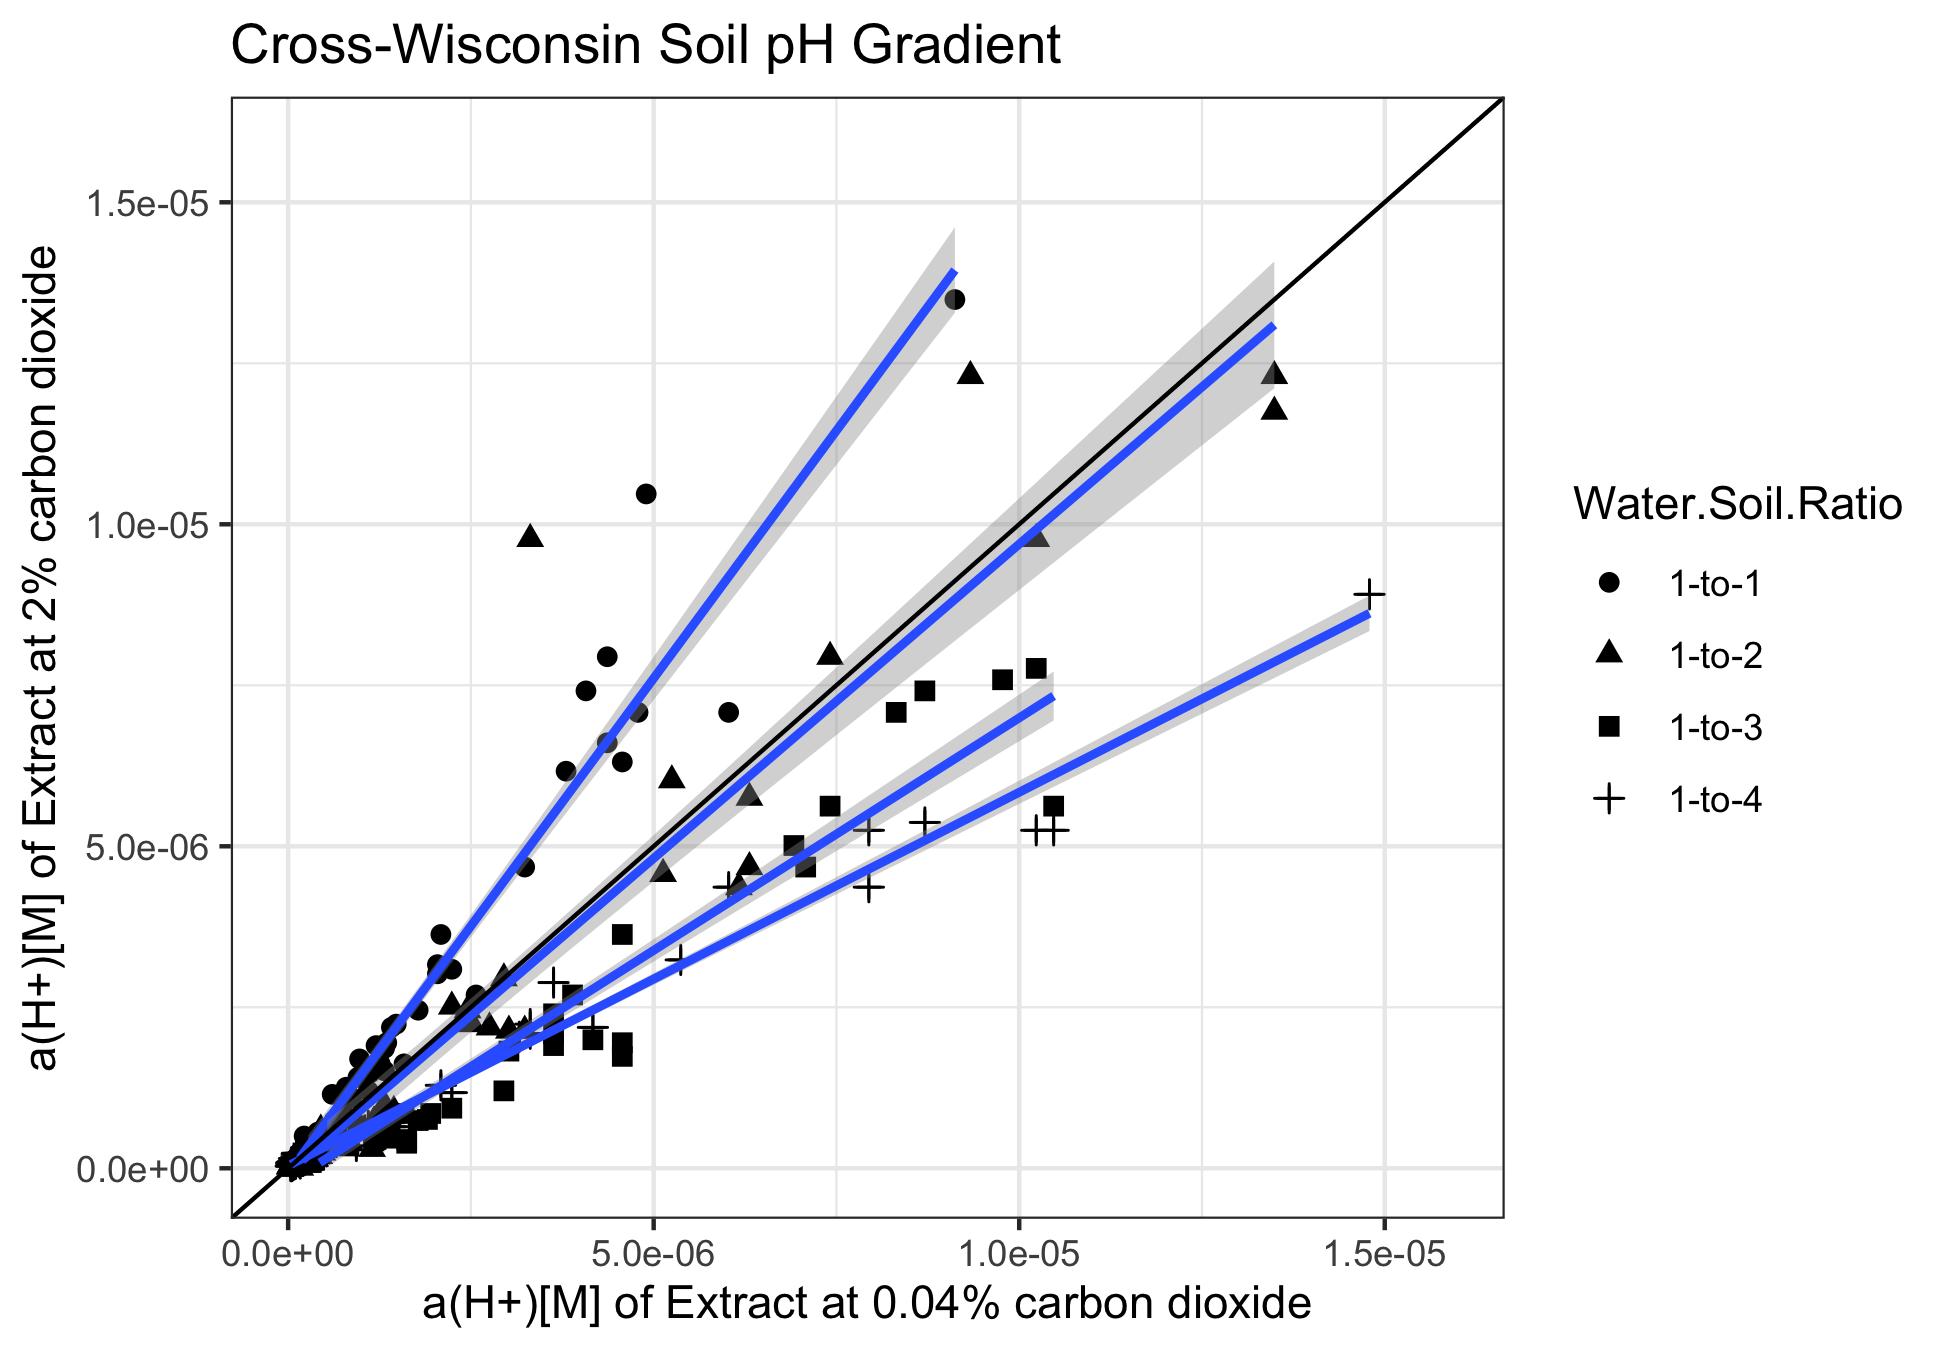
\includegraphics{output-rmd/wisc-stand-sim-soil-hplus-bw-1.png}

\hypertarget{spooner-1}{%
\subsubsection{Spooner}\label{spooner-1}}

\begin{Shaded}
\begin{Highlighting}[]
\NormalTok{q3.bw <-}\StringTok{ }\KeywordTok{qplot}\NormalTok{(}\DataTypeTok{data =}\NormalTok{ dat.spooner, }\DataTypeTok{x =}\NormalTok{ Lab.CO2.pH, }\DataTypeTok{y =}\NormalTok{ High.CO2.pH, }\DataTypeTok{shape =}\NormalTok{ Water.Soil.Ratio) }\OperatorTok{+}\StringTok{ }\KeywordTok{geom_point}\NormalTok{(}\DataTypeTok{size=}\DecValTok{2}\NormalTok{) }\OperatorTok{+}
\StringTok{  }\KeywordTok{theme_bw}\NormalTok{() }\OperatorTok{+}\StringTok{ }\KeywordTok{geom_smooth}\NormalTok{(}\DataTypeTok{method =} \StringTok{"glm"}\NormalTok{) }\OperatorTok{+}\StringTok{ }
\StringTok{  }\KeywordTok{geom_abline}\NormalTok{(}\DataTypeTok{slope =} \DecValTok{1}\NormalTok{, }\DataTypeTok{intercept =} \DecValTok{0}\NormalTok{, }\DataTypeTok{color =} \StringTok{"black"}\NormalTok{) }\OperatorTok{+}\StringTok{ }
\StringTok{  }\KeywordTok{labs}\NormalTok{(}\DataTypeTok{color=}\StringTok{'Solution-to-Soil }\CharTok{\textbackslash{}n}\StringTok{ Ratio by Mass'}\NormalTok{, }
       \DataTypeTok{x =} \StringTok{"pH of Extract at 0.04% carbon dioxide"}\NormalTok{, }
       \DataTypeTok{y =} \StringTok{"pH of Extract at 2% carbon dioxide"}\NormalTok{)  }\OperatorTok{+}\StringTok{ }
\StringTok{  }\KeywordTok{ggtitle}\NormalTok{(}\StringTok{"Long-term Soil pH Manipulation"}\NormalTok{)}
\NormalTok{q3.bw}
\end{Highlighting}
\end{Shaded}

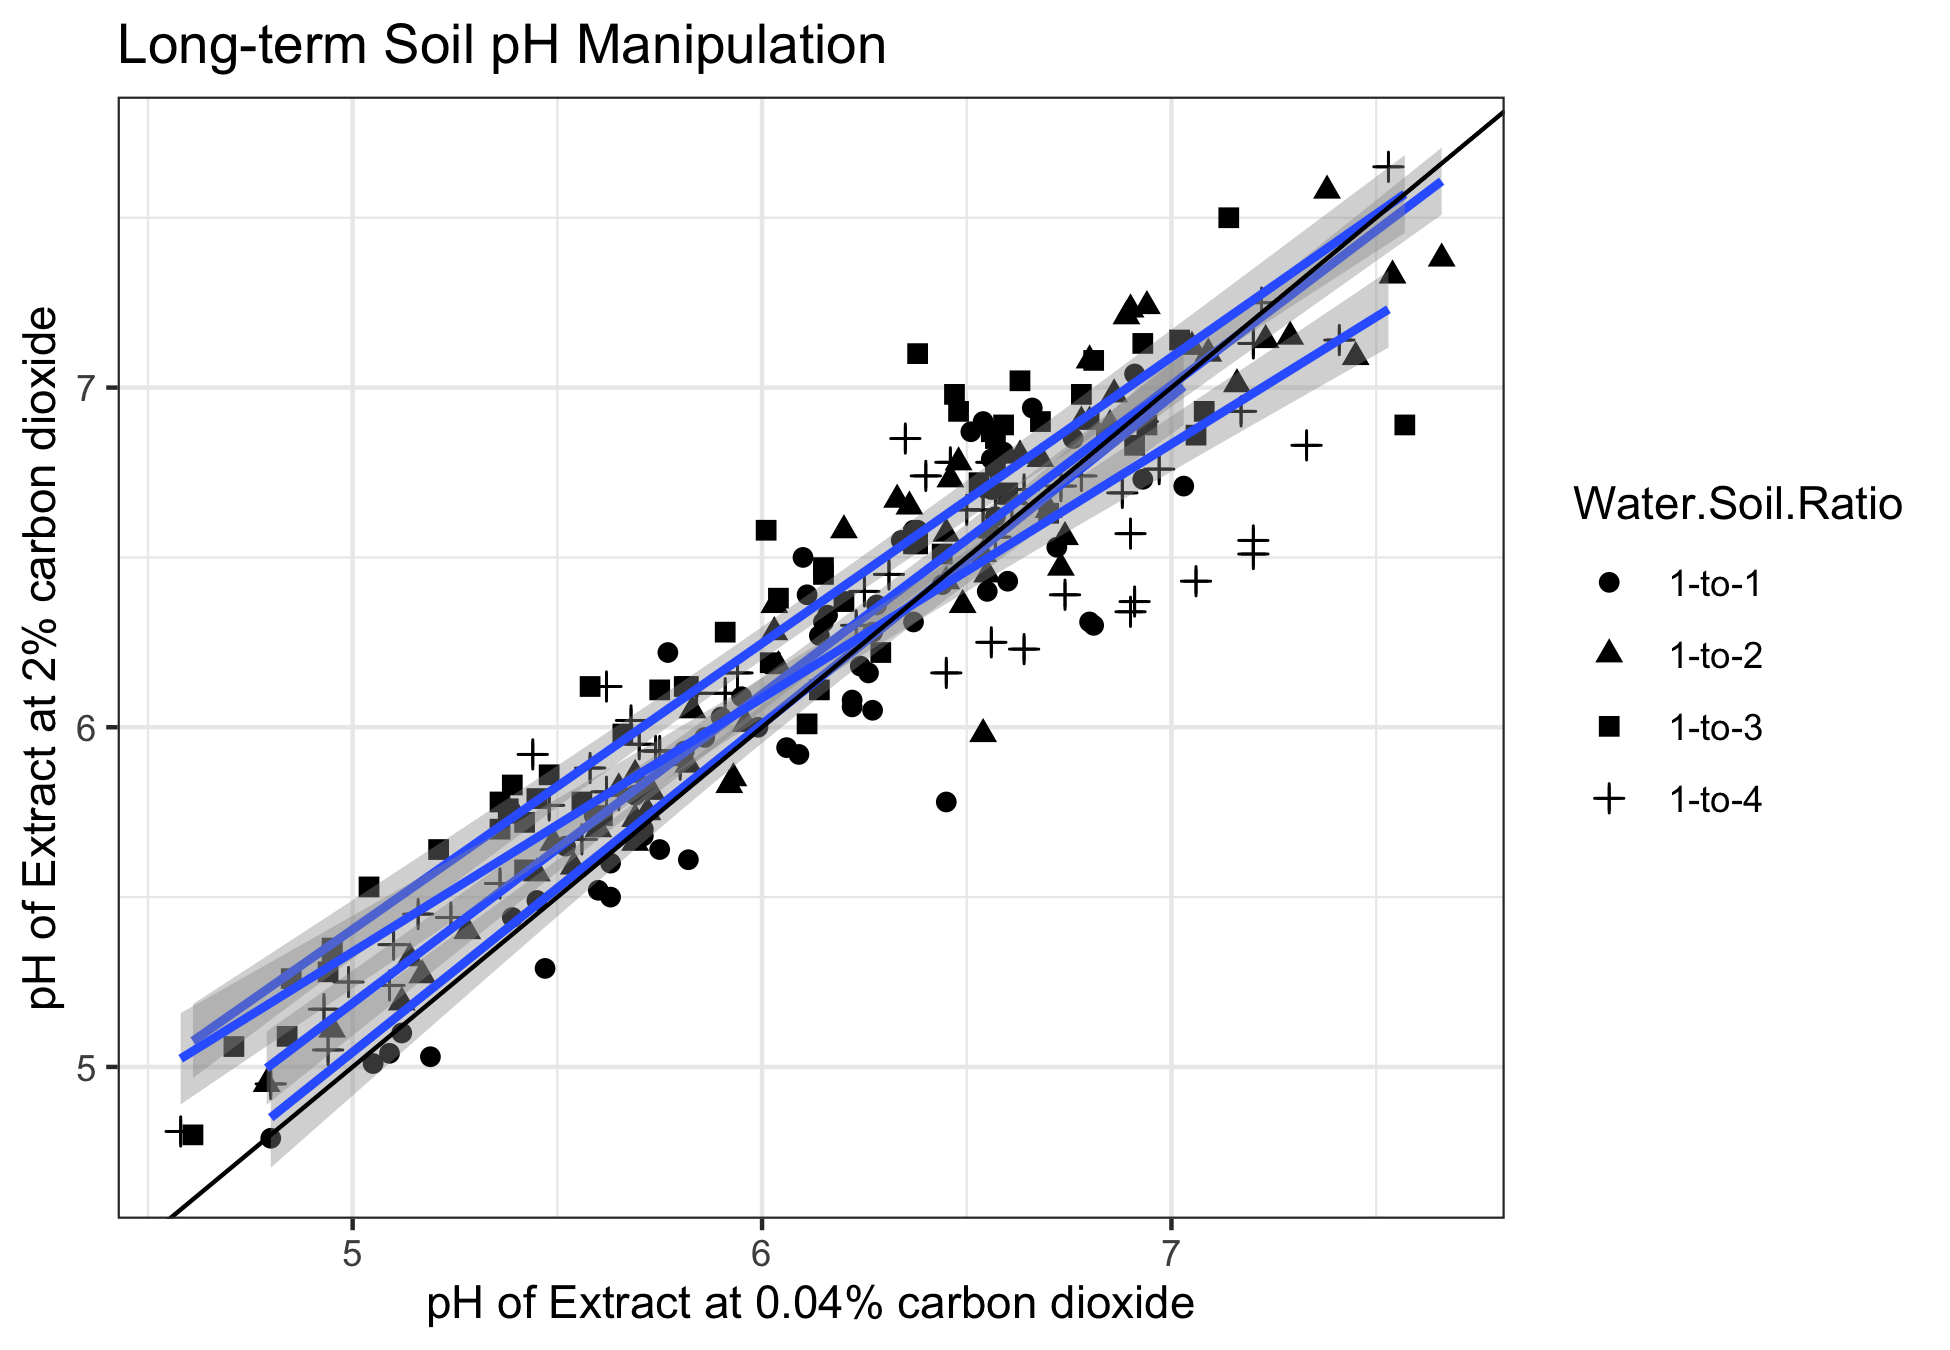
\includegraphics{output-rmd/spooner-stand-sim-soil-ph-bw-1.png}

\begin{Shaded}
\begin{Highlighting}[]
\NormalTok{q4.bw <-}\StringTok{ }\KeywordTok{qplot}\NormalTok{(}\DataTypeTok{data =}\NormalTok{ dat.spooner, }\DataTypeTok{x =} \DecValTok{10}\OperatorTok{^-}\NormalTok{Lab.CO2.pH, }\DataTypeTok{y =} \DecValTok{10}\OperatorTok{^-}\NormalTok{High.CO2.pH, }\DataTypeTok{shape =}\NormalTok{ Water.Soil.Ratio) }\OperatorTok{+}\StringTok{ }\KeywordTok{geom_point}\NormalTok{(}\DataTypeTok{size=}\DecValTok{2}\NormalTok{) }\OperatorTok{+}\StringTok{ }\KeywordTok{scale_x_continuous}\NormalTok{(}\DataTypeTok{limits =} \KeywordTok{c}\NormalTok{(}\DecValTok{10}\OperatorTok{^-}\FloatTok{8.1}\NormalTok{, }\DecValTok{10}\OperatorTok{^-}\FloatTok{4.8}\NormalTok{)) }\OperatorTok{+}\StringTok{ }\KeywordTok{scale_y_continuous}\NormalTok{(}\DataTypeTok{limits =} \KeywordTok{c}\NormalTok{(}\DecValTok{10}\OperatorTok{^-}\FloatTok{8.1}\NormalTok{, }\DecValTok{10}\OperatorTok{^-}\FloatTok{4.8}\NormalTok{)) }\OperatorTok{+}\StringTok{ }\KeywordTok{theme_bw}\NormalTok{() }\OperatorTok{+}\StringTok{ }\KeywordTok{geom_smooth}\NormalTok{(}\DataTypeTok{method =} \StringTok{"glm"}\NormalTok{) }\OperatorTok{+}\StringTok{ }\KeywordTok{geom_abline}\NormalTok{(}\DataTypeTok{slope =} \DecValTok{1}\NormalTok{, }\DataTypeTok{intercept =} \DecValTok{0}\NormalTok{, }\DataTypeTok{color =} \StringTok{"black"}\NormalTok{)}\OperatorTok{+}
\StringTok{  }\KeywordTok{labs}\NormalTok{(}\DataTypeTok{color=}\StringTok{'Solution-to-Soil }\CharTok{\textbackslash{}n}\StringTok{ Ratio by Mass'}\NormalTok{, }
       \DataTypeTok{x =} \StringTok{"a(H+)[M] of Extract at 0.04% carbon dioxide"}\NormalTok{, }
       \DataTypeTok{y =} \StringTok{"a(H+)[M] of Extract at 2% carbon dioxide"}\NormalTok{) }\OperatorTok{+}\StringTok{ }
\StringTok{  }\KeywordTok{ggtitle}\NormalTok{(}\StringTok{"Long-term Soil pH Manipulation"}\NormalTok{)}
\NormalTok{q4.bw}
\end{Highlighting}
\end{Shaded}

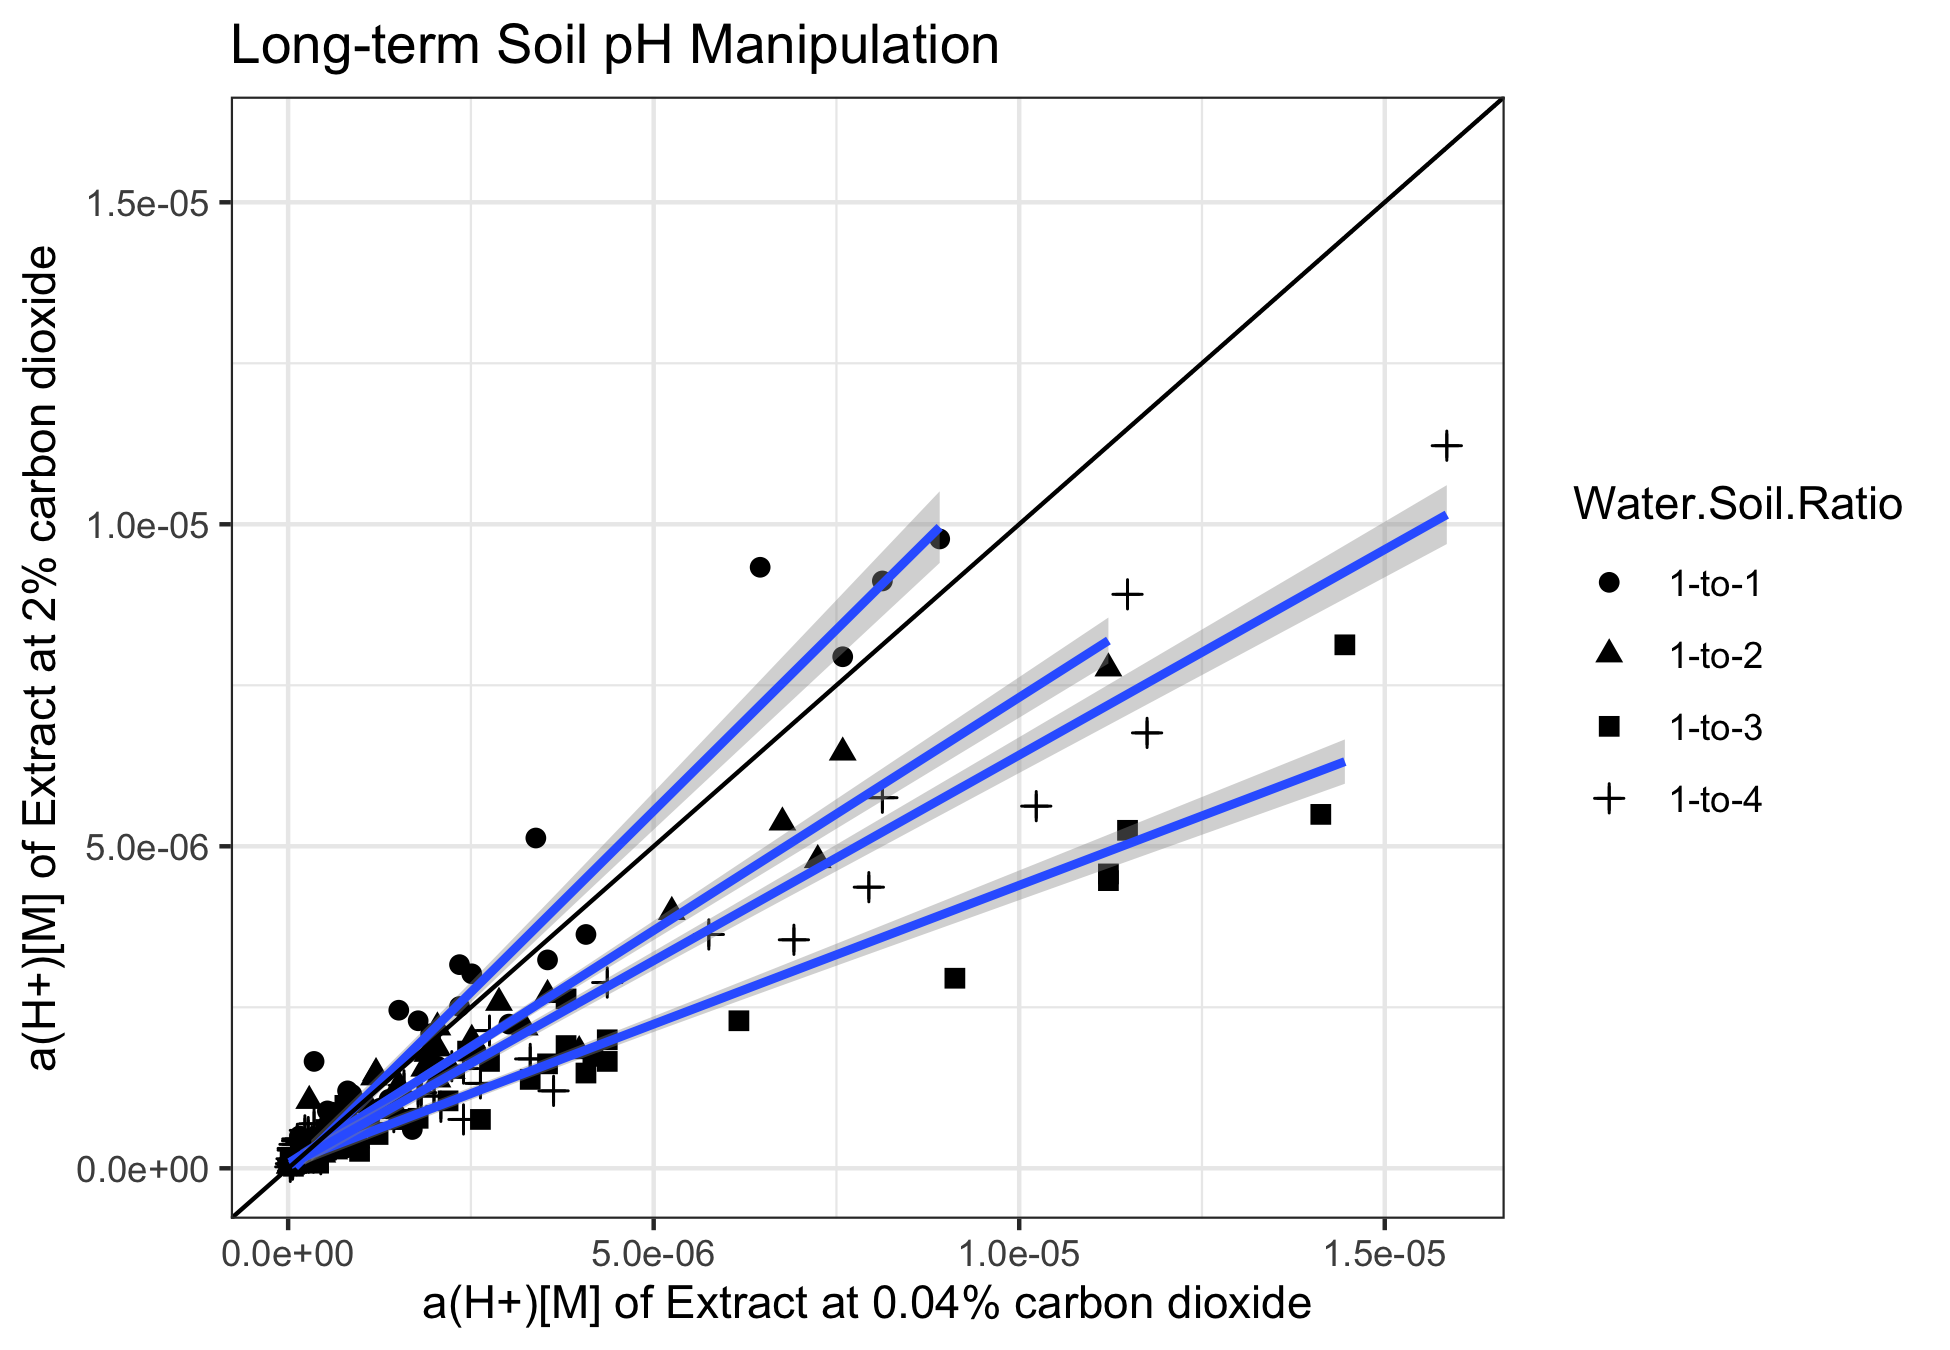
\includegraphics{output-rmd/spooner-stand-sim-soil-hplus-bw-1.png}

\hypertarget{grid-of-multifactorial-plots-1}{%
\subsubsection{Grid of Multifactorial
Plots}\label{grid-of-multifactorial-plots-1}}

\begin{Shaded}
\begin{Highlighting}[]
\KeywordTok{plot_grid}\NormalTok{(q1.bw, q2.bw, q3.bw, q4.bw) }
\end{Highlighting}
\end{Shaded}

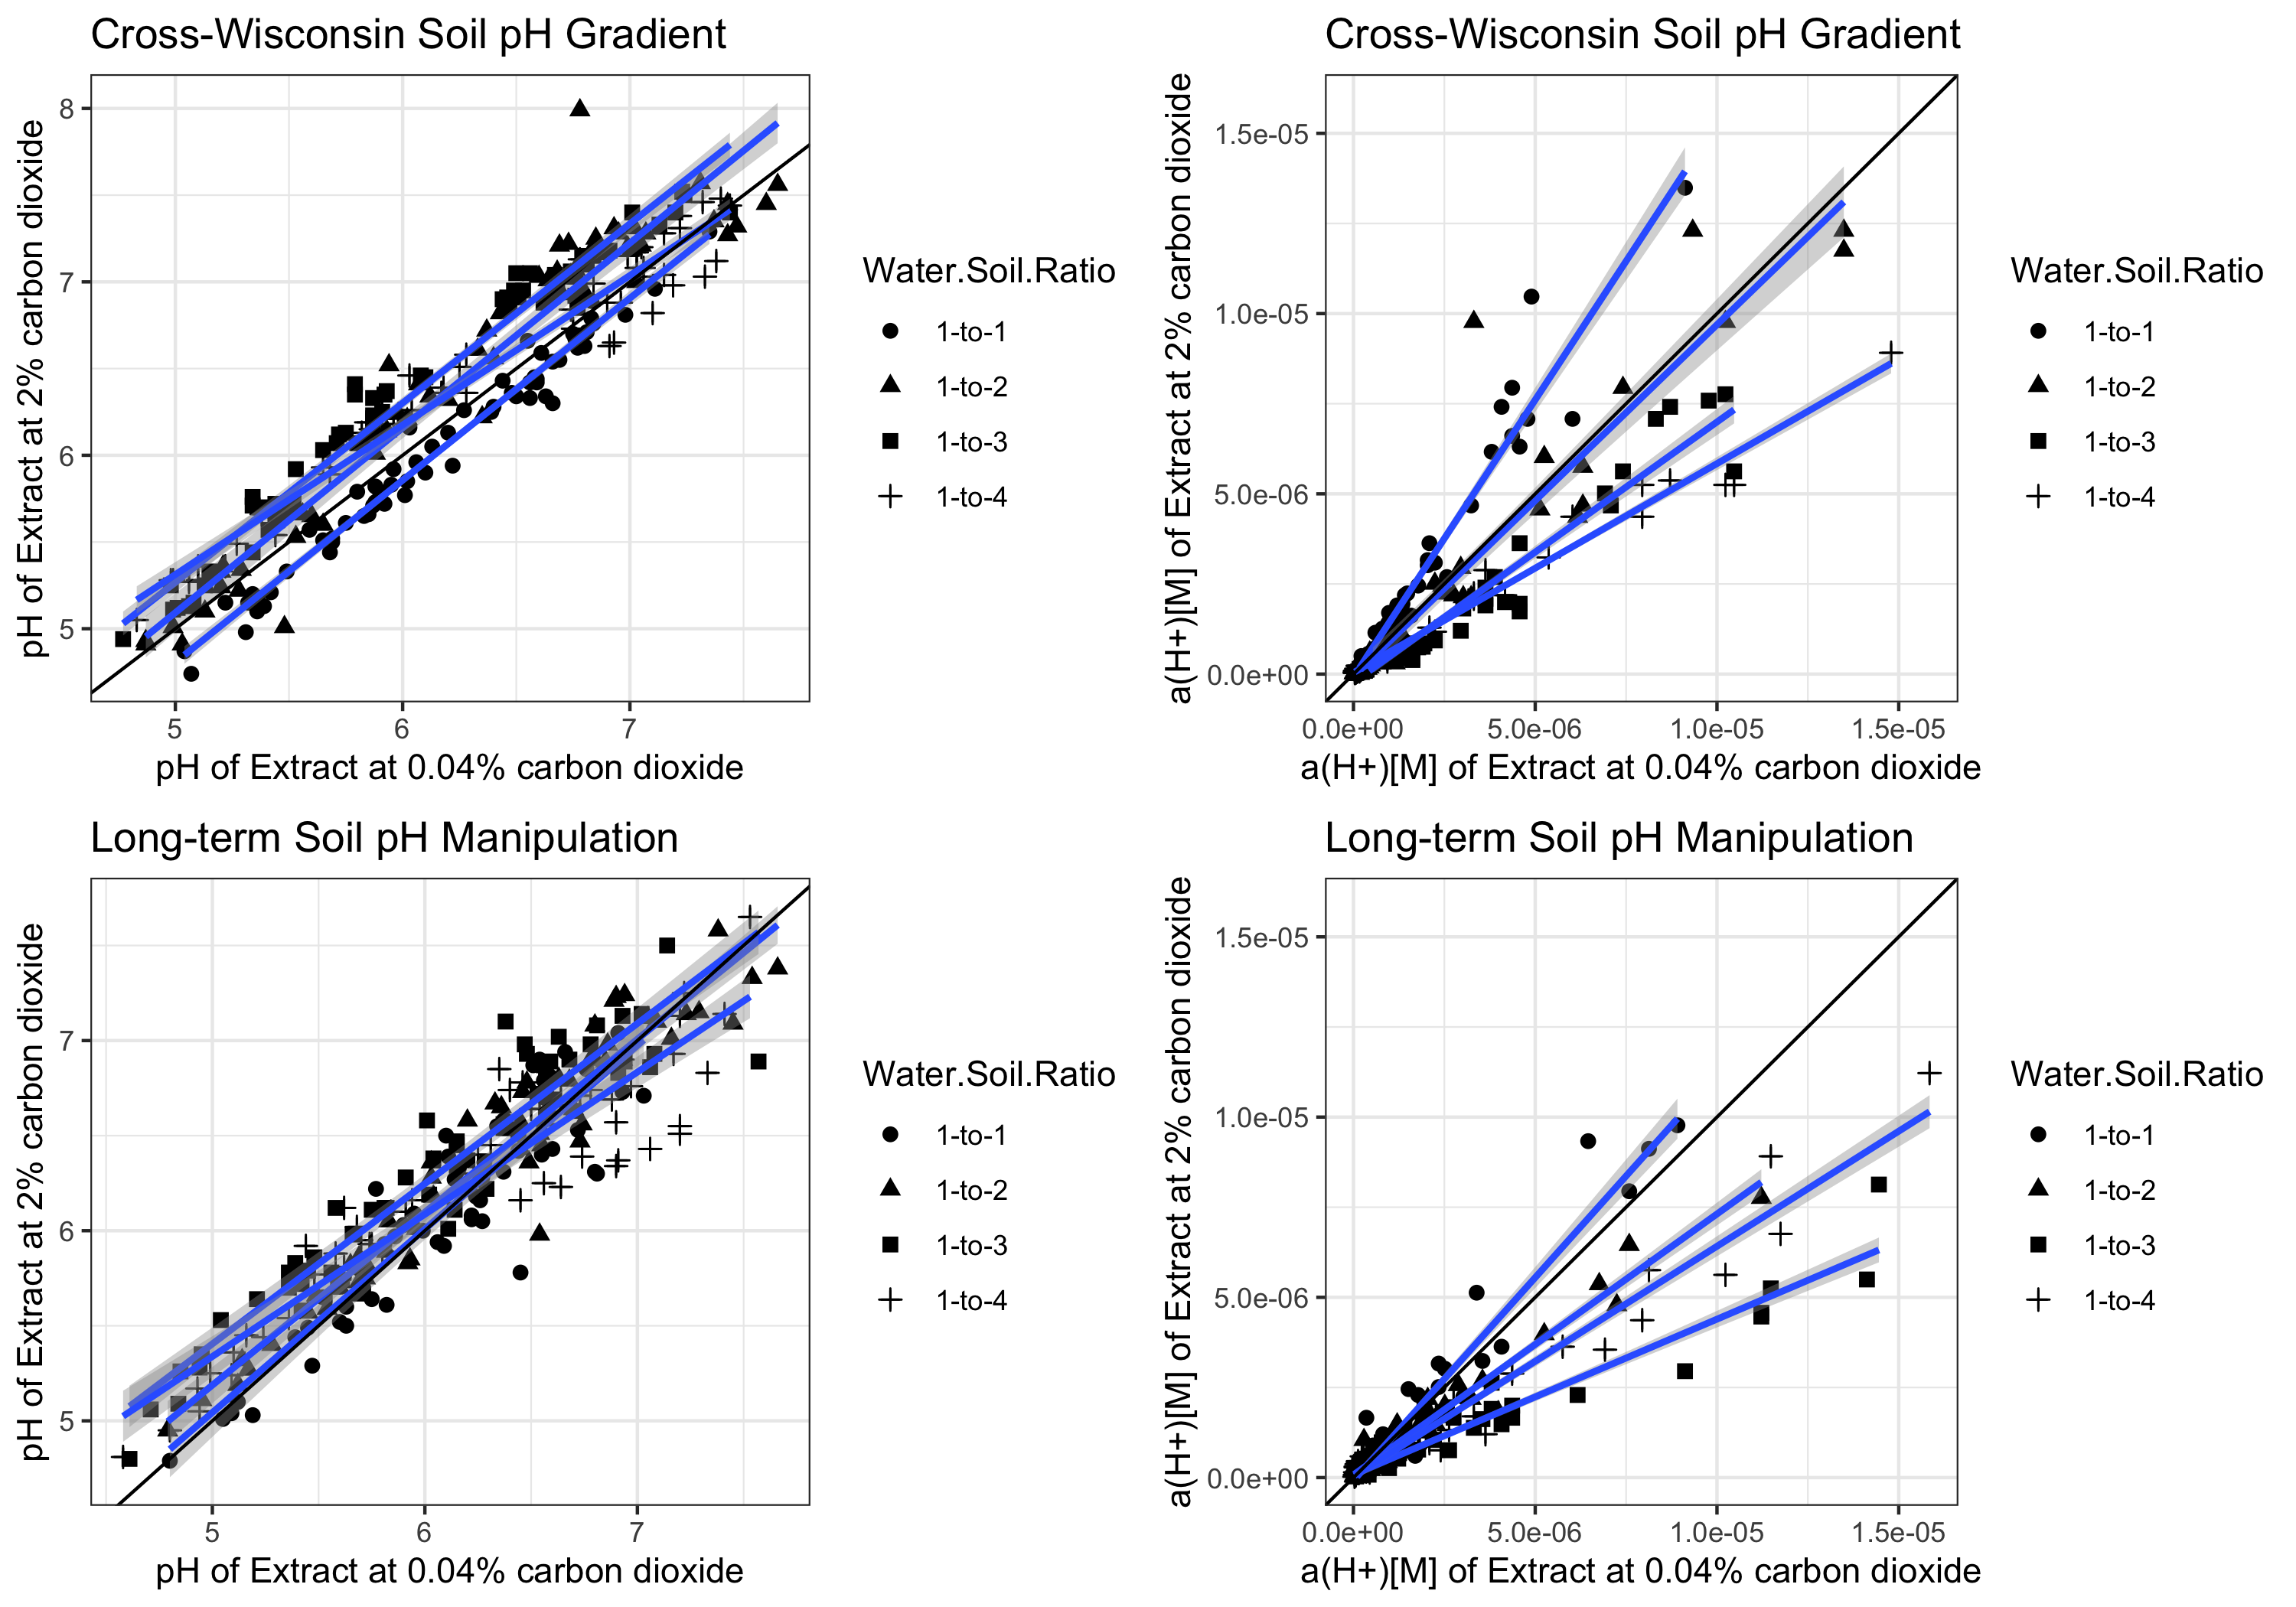
\includegraphics{output-rmd/multifactoral-grid-ph-bw-1.png}

\hypertarget{microbial-paper}{%
\section{MICROBIAL PAPER}\label{microbial-paper}}

\hypertarget{biom-metadata}{%
\subsection{Biom + Metadata}\label{biom-metadata}}

Let's load all these packages.

\begin{Shaded}
\begin{Highlighting}[]
\CommentTok{# Intall:}
\CommentTok{# BiocManager::install("phyloseq")}
\CommentTok{# Load libraries}
\KeywordTok{library}\NormalTok{(phyloseq)}
\CommentTok{#library(dada2)}
\KeywordTok{library}\NormalTok{(ggplot2)}
\KeywordTok{library}\NormalTok{(RColorBrewer)}
\KeywordTok{library}\NormalTok{(vegan)}
\end{Highlighting}
\end{Shaded}

Here we'll load in the microbial data.

\begin{Shaded}
\begin{Highlighting}[]
\CommentTok{# Import sequence processing table and check it out}
\CommentTok{# How many sequences were retained at each step?}
\NormalTok{track =}\StringTok{ }\KeywordTok{readRDS}\NormalTok{(}\StringTok{"reads/track.rds"}\NormalTok{)}
\NormalTok{track}
\end{Highlighting}
\end{Shaded}

\begin{verbatim}
##                           input filtered denoised tabled nonchim
## 001-K1-0-17_S1_          182876   113727    95159  95159   89297
## 002-K1-17-45_S2_          81260    51682    42307  42307   41748
## 003-K1-45-60_S3_          55300    27171    20888  20888   20171
## 004-K2-Muck_S4_          108860    71520    57380  57380   53443
## 005-K3-0-15_S5_          135686    71730    54482  54482   51936
## 006-K3-15-35_S6_         107464    37348    23576  23576   23486
## 007-K3-35-50_S7_         115786    78875    65044  65044   62650
## 008-K4-0-15_S8_          100152    19285     8619   8619    8556
## 009-K4-15-30_S9_          57577    35582    29993  29993   29051
## 010-K4-30-50_S10_         93763    46765    38406  38406   37402
## 011-R1-0-27_S11_         128413    40030    21838  21838   21737
## 012-R1-27-50_S12_        108524    67801    57776  57776   56713
## 013-R1-50-70_S13_        101327    44743    37288  37288   36691
## 014-R2-0-30_S14_          98020    50303    34370  34370   33980
## 015-R2-30-45_S15_        144651    83427    67939  67939   66910
## 016-R2-45-60_S16_        130070    34111    25167  25167   25018
## 017-R2-60-100_S17_       107756    58066    49565  49565   47991
## 018-R3-0-20_S18_          79325    34393    20386  20386   20326
## 019-R3-20-30_S19_        101494    43254    33039  33039   32370
## 020-M1-0-31_S20_          81090    44031    28164  28164   28059
## 021-M1-31-50_S21_        123202    32323    19729  19729   19466
## 022-M1-50-70_S22_        115300    58825    50270  50270   48700
## 023-M2-0-24_S23_          69786    37765    25211  25211   25211
## 024-M2-24-38_S24_         66500     4392     1360   1360    1360
## 025-M2-38-55_S25_         72317    11461     6401   6401    6401
## 026-M3-0-15_S26_          93907    58097    44706  44706   43995
## 027-M3-15-30_S27_        113189    69066    58961  58961   55617
## 028-S-0-30_S28_           84651    45676    33139  33139   32957
## 029-S-30-60_S29_          93210    60904    51755  51755   49984
## 030-H1-0-30_S30_          90750    46239    27822  27822   27668
## 031-H1-30-40_S31_         86567    30139    17938  17938   17938
## 032-H1-40-60_S32_        105640    67558    59240  59240   57478
## 033-H2-0-30_S33_          87099    16339     6348   6348    6348
## 034-H2-30-60_S34_         83980    49334    41732  41732   40567
## 035-A249-0-35_S35_       171995    99802    78097  78097   76177
## 036-A249-35-60_S36_      150886    31831    20121  20121   19889
## 037-A341-0-33_S37_        85427    58108    43652  43652   42498
## 038-A341-33-55_S38_      152238    37509    22947  22947   22729
## 039-A341-55-75_S39_      136405    86536    70615  70615   66543
## 040-A341-75-85_S40_      136079    73684    61036  61036   57498
## 041-L2-0-23_S41_         159454    43258    23094  23094   23094
## 042-L2-23-45_S42_        122710    65865    49028  49028   47069
## 043-L3-0-12_S43_          86274    17177     8855   8855    8855
## 044-L3-12-20_S44_        132616    73576    55701  55701   55220
## 045-L3-20-40_S45_         80337    50489    40351  40351   39803
## 046-L4-0-10_S46_          99581    22005     9226   9226    9171
## 047-L4-10-20_S47_         91215    50684    32790  32790   31661
## 048-L4-20-40_S48_        119412    50107    33518  33518   32534
## 049-W3-Compost_S49_      180030    78201    58381  58381   52148
## 050-W4-0-28_S50_         104694    18856     9956   9956    9956
## 051-W4-28-45_S51_        247394   151323   128651 128651  119735
## 052-W4-45-55_S52_        115897    75634    62731  62731   61321
## 053-W5-0-35_S53_         103001    54100    37307  37307   36937
## 054-W5-35-65_S54_        105301    69483    54655  54655   51766
## 055-W7-0-15_S55_          89996    48631    33299  33299   32938
## 056-W7-15-30_S56_         66065    21643    13343  13343   13343
## 057-P1-0-30_S57_          89999    57426    41822  41822   41207
## 058-P1-30-45_S58_        109185    15843     8812   8812    8812
## 059-P1-45-55_S59_         92847    61590    51573  51573   50559
## 060-P2-0-20_S60_         107565    53905    36050  36050   35670
## 061-P2-20-45_S61_        176157    42505    23826  23826   23486
## 062-P2-45-55_S62_        136875    73794    57793  57793   55732
## 063-P4-0-25_S63_         146085    56463    34722  34722   34268
## 064-P4-25-35_S64_        153343    95555    73081  73081   68963
## 065-P4-35-50_S65_        120945    69145    50362  50362   48655
## 181-Sp11-Cr31-0-20_S66_  107462    27633    10675  10675   10675
## 182-Sp11-Cr32-0-16_S67_   88842    21116     7352   7352    7352
## 183-Sp11-Cr33-0-20_S68_   48207    17300     6739   6739    6739
## 184-Sp12-Cr34-0-16_S69_   91437    57258    37259  37259   37078
## 185-Sp12-Cr35-0-18_S70_  102991    61552    39530  39530   38480
## 186-Sp12-Cr36-0-20_S71_   74281    17619     6050   6050    6050
## 187-Sp13-Cr37-0-20_S72_   87916    35459    16580  16580   16570
## 188-Sp13-Cr38-0-20_S73_   92749    48058    30511  30511   30290
## 189-Sp13-Cr39-0-19_S74_  120274    64100    43911  43911   43536
## 190-Sp14-Cr40-0-17_S75_  147563    19324     7700   7700    7700
## 191-Sp14-Cr41-0-18_S76_  123615    76067    58444  58444   57514
## 192-Sp14-Cr42-0-20_S77_   95005    57765    40490  40490   40337
## 193-Sp15-Cr43-0-18_S78_  117756    55650    40950  40950   40238
## 194-Sp15-Cr44-0-17_S79_  144523    84487    71381  71381   68362
## 195-Sp15-Cr45-0-20_S80_  108008    49459    32985  32985   32567
## 196-Sp16-Cr46-0-20_S81_   82746    25675     8942   8942    8942
## 197-Sp16-Cr47-0-17_S82_  107765    64753    42508  42508   42356
## 198-Sp16-Cr48-0-20_S83_  115552    33125    14483  14483   14483
## 199-Sp17-Cr49-0-20_S84_  120659    64605    52183  52183   50940
## 200-Sp17-Cr50-0-18_S85_  161957    82546    62933  62933   59863
## 201-Sp17-Cr51-0-18_S86_  109479    10752     4159   4159    4159
## 202-Sp18-Cr52-0-18_S87_  113065    72492    49565  49565   49262
## 203-Sp18-Cr53-0-19_S88_   92639    33398    15743  15743   15715
## 204-Sp18-Cr54-0-20_S89_   95422    59781    38645  38645   38431
## 205-Sp19-Cr55-0-20_S90_  204505   101955    73534  73534   71731
## 206-Sp19-Cr56-0-18_S91_   98520     7220     2276   2276    2276
## 207-Sp19-Cr57-0-18_S92_   97994    36745    19184  19184   19184
## 208-Sp20-Cr58-0-20_S93_   81724    36655    17796  17796   17796
## 209-Sp20-Cr59-0-19_S94_  148052    84565    54466  54466   53727
## 210-Sp20-Cr60-0-20_S95_   66841    40391    25375  25375   25288
## 211-Sp1-Cr1-0-20_S96_    134100    15037     6086   6086    6086
## 212-Sp1-Cr2-0-20_S97_     66264    14952     7640   7640    7537
## 213-Sp1-Cr3-0-20_S98_     71197    33638    23553  23553   19873
## 214-Sp2-Cr4-0-20_S99_     64668    32062    19681  19681   19681
## 215-Sp2-Cr5-0-20_S100_    59680     9677     3727   3727    3727
## 216-Sp2-Cr6-0-20_S101_    83270    51845    41388  41388   41287
## 217-Sp3-Cr7-0-20_S102_    73671    46034    29507  29507   29332
## 218-Sp3-Cr8-0-20_S103_    97858    53712    31869  31869   31707
## 219-Sp3-Cr9-0-20_S104_    97545    61866    40989  40989   40599
## 220-Sp4-Cr10-0-20_S105_   71516    34617    18555  18555   18555
## 221-Sp4-Cr11-0-20_S106_   63790    17585     6625   6625    6625
## 222-Sp4-Cr12-0-20_S107_  117411    78366    57338  57338   56779
## 223-Sp5-Cr13-0-20_S108_  108733    20176     6204   6204    6204
## 224-Sp5-Cr14-0-20_S109_   90829    58242    40371  40371   40169
## 225-Sp5-Cr15-0-20_S110_   64613    28212    13220  13220   13143
## 226-Sp6-Cr16-0-15_S111_   82006    19304     7464   7464    7464
## 227-Sp6-Cr17-0-20_S112_   76389    49052    30022  30022   29835
## 228-Sp6-Cr18-0-20_S113_   90349    34880    16346  16346   16247
## 229-Sp7-Cr19-0-20_S114_  115919    64710    51544  51544   50690
## 230-Sp7-Cr20-0-20_S115_   74230    18776    11523  11523   11499
## 231-Sp7-Cr21-0-13_S116_   75045    12521     5294   5294    5294
## 232-Sp8-Cr22-0-20_S117_  141073    69721    45560  45560   45482
## 233-Sp8-Cr23-0-20_S118_  110558    45709    26455  26455   26417
## 234-Sp8-Cr24-0-20_S119_   61465    37231    24321  24321   24273
## 235-Sp9-Cr25-0-15_S120_   83784    41544    22254  22254   22165
## 236-Sp9-Cr26-0-20_S121_   80446    48274    32007  32007   31862
## 237-Sp9-Cr27-0-15_S122_   80498    21827     8729   8729    8729
## 238-Sp10-Cr28-0-20_S123_  75603    36729    24170  24170   24160
## 239-Sp10-Cr29-0-15_S124_  84146    43982    30468  30468   30468
## 240-Sp10-Cr30-0-20_S125_  85612    12867     4856   4856    4856
## 241-S-0-30-Dry_S126_      81180    46857    39598  39598   39224
\end{verbatim}

\begin{Shaded}
\begin{Highlighting}[]
\CommentTok{# Import final otu table}
\NormalTok{OTUs =}\StringTok{ }\KeywordTok{readRDS}\NormalTok{(}\StringTok{"reads/OTUtab.nochim.rds"}\NormalTok{)}
\CommentTok{# Change rows and columns so taxa are rows}
\NormalTok{OTUs =}\StringTok{ }\KeywordTok{t}\NormalTok{(OTUs)}
\CommentTok{# Import as phyloseq object table}
\NormalTok{otutab =}\StringTok{ }\KeywordTok{otu_table}\NormalTok{(OTUs, }\DataTypeTok{taxa_are_rows=}\OtherTok{TRUE}\NormalTok{)}
\KeywordTok{head}\NormalTok{(otutab)}
\end{Highlighting}
\end{Shaded}

\begin{verbatim}
## OTU Table:          [6 taxa and 126 samples]
##                      taxa are rows
##                                                                                                                                                                                                                                                           001-K1-0-17_S1__F_filt.fastq.gz
## CGTAGGGCGCAAGCGTTATCCGGAATTATTGGGCGTAAAGAGCTCGTAGGCGGTTTGTCGCGTCTGCCGTGAAAGTCCGGGGCTCAACTCCGGATCTGCGGTGGGTACGGGCAGACTAGAGTGATGTAGGGGAGACTGGAATTCCTGGTGTAGCGGTGAAATGCGCAGATATCAGGAGGAACACCGATGGCGAAGGCAGGTCTCTGGGCATTAACTGACGCTGAGGAGCGAAAGCATGGGGAGCGAACA                               0
## CAGAGGTCTCAAGCGTTGTTCGGATTCATTGGGCGTAAAGGGTGCGTAGGCGGCGCGGTAAGTCGGGTGTGAAATCTCGGAGCTTAACTCCGAAACTGCATTCGATACTGCCGTGCTTGAGGACTGGAGAGGAGACTGGAATTTACGGTGTAGCGGTGAAATGCGTAGATATCGTAAGGAAGACCAGTGGCGAAGGCGGGTCTCTGGACAGTTCCTGACGCTGAGGCACGAAGGCCAGGGGAGCAAACG                             461
## GTAGGGGGCAAGCGTTATCCAGATTTACTGGGCGTAAAGCGCGTGTAGGCGGCTGGTTAGGTGTGATGTGAAATCTTCCGGCTCAACCGGAAAACTGCATTGCAAACCGGCCTGGCTAGAGTGCAGGAGAGGGAAGCGGAATTCCAGGTGTAGCGGTGAAATGCGTAGATATCTGGAGGAACACCAGTGGCGAAGGCGGCTTCCTGGCCTGCAACTGACGCTGAGACGCGAAAGCGTGGGGAGCGAAC                              157
## CGAAGGGGGCTAGCGTTGCTCGGAATCACTGGGCGTAAAGGGTGCGTAGGCGGGTCTTTAAGTCAGGGGTGAAATCCTGGAGCTCAACTCCAGAACTGCCTTTGATACTGAAGATCTTGAGTTCGGGAGAGGTGAGTGGAACTGCGAGTGTAGAGGTGAAATTCGTAGATATTCGCAAGAACACCAGTGGCGAAGGCGGCTCACTGGCCCGATACTGACGCTGAGGCACGAAAGCGTGGGGAGCAAACA                             482
## CGTAGGTGGCAAGCGTTGTCCGGATTTACTGGGCGTAAAGAGCGCGCAGGCGGTCGTTCAAGTCGCGTGTGAAAGCCCCCGGCTCAACTGGGGAGGGTCACGCGATACTGATCGACTCGAAGGCAGGAGAGGGTAGTGGAATTCCCGGTGTAGTGGTGAAATGCGTAGATATCGGGAGGAACACCAGTGGCGAAGGCGACTACCTGGCCTGTTCTTGACGCTGAGGCGCGAAAGCTAGGGGAGCAAACG                               0
## CAGAGGTCTCAAGCGTTGTTCGGATTCATTGGGCGTAAAGGGTGCGTAGGCGGCGCGGTAAGTCGGGTGTGAAATCTCGGGGCTTAACTCCGAAACTGCATTCGATACTGCCGTGCTTGAGGACTGGAGAGGAGACTGGAATTTACGGTGTAGCGGTGAAATGCGTAGATATCGTAAGGAAGACCAGTGGCGAAGGCGGGTCTCTGGACAGTTCCTGACGCTGAGGCACGAAGGCCAGGGGAGCAAACG                             181
##                                                                                                                                                                                                                                                           002-K1-17-45_S2__F_filt.fastq.gz
## CGTAGGGCGCAAGCGTTATCCGGAATTATTGGGCGTAAAGAGCTCGTAGGCGGTTTGTCGCGTCTGCCGTGAAAGTCCGGGGCTCAACTCCGGATCTGCGGTGGGTACGGGCAGACTAGAGTGATGTAGGGGAGACTGGAATTCCTGGTGTAGCGGTGAAATGCGCAGATATCAGGAGGAACACCGATGGCGAAGGCAGGTCTCTGGGCATTAACTGACGCTGAGGAGCGAAAGCATGGGGAGCGAACA                                0
## CAGAGGTCTCAAGCGTTGTTCGGATTCATTGGGCGTAAAGGGTGCGTAGGCGGCGCGGTAAGTCGGGTGTGAAATCTCGGAGCTTAACTCCGAAACTGCATTCGATACTGCCGTGCTTGAGGACTGGAGAGGAGACTGGAATTTACGGTGTAGCGGTGAAATGCGTAGATATCGTAAGGAAGACCAGTGGCGAAGGCGGGTCTCTGGACAGTTCCTGACGCTGAGGCACGAAGGCCAGGGGAGCAAACG                              369
## GTAGGGGGCAAGCGTTATCCAGATTTACTGGGCGTAAAGCGCGTGTAGGCGGCTGGTTAGGTGTGATGTGAAATCTTCCGGCTCAACCGGAAAACTGCATTGCAAACCGGCCTGGCTAGAGTGCAGGAGAGGGAAGCGGAATTCCAGGTGTAGCGGTGAAATGCGTAGATATCTGGAGGAACACCAGTGGCGAAGGCGGCTTCCTGGCCTGCAACTGACGCTGAGACGCGAAAGCGTGGGGAGCGAAC                               522
## CGAAGGGGGCTAGCGTTGCTCGGAATCACTGGGCGTAAAGGGTGCGTAGGCGGGTCTTTAAGTCAGGGGTGAAATCCTGGAGCTCAACTCCAGAACTGCCTTTGATACTGAAGATCTTGAGTTCGGGAGAGGTGAGTGGAACTGCGAGTGTAGAGGTGAAATTCGTAGATATTCGCAAGAACACCAGTGGCGAAGGCGGCTCACTGGCCCGATACTGACGCTGAGGCACGAAAGCGTGGGGAGCAAACA                              159
## CGTAGGTGGCAAGCGTTGTCCGGATTTACTGGGCGTAAAGAGCGCGCAGGCGGTCGTTCAAGTCGCGTGTGAAAGCCCCCGGCTCAACTGGGGAGGGTCACGCGATACTGATCGACTCGAAGGCAGGAGAGGGTAGTGGAATTCCCGGTGTAGTGGTGAAATGCGTAGATATCGGGAGGAACACCAGTGGCGAAGGCGACTACCTGGCCTGTTCTTGACGCTGAGGCGCGAAAGCTAGGGGAGCAAACG                                0
## CAGAGGTCTCAAGCGTTGTTCGGATTCATTGGGCGTAAAGGGTGCGTAGGCGGCGCGGTAAGTCGGGTGTGAAATCTCGGGGCTTAACTCCGAAACTGCATTCGATACTGCCGTGCTTGAGGACTGGAGAGGAGACTGGAATTTACGGTGTAGCGGTGAAATGCGTAGATATCGTAAGGAAGACCAGTGGCGAAGGCGGGTCTCTGGACAGTTCCTGACGCTGAGGCACGAAGGCCAGGGGAGCAAACG                              247
##                                                                                                                                                                                                                                                           003-K1-45-60_S3__F_filt.fastq.gz
## CGTAGGGCGCAAGCGTTATCCGGAATTATTGGGCGTAAAGAGCTCGTAGGCGGTTTGTCGCGTCTGCCGTGAAAGTCCGGGGCTCAACTCCGGATCTGCGGTGGGTACGGGCAGACTAGAGTGATGTAGGGGAGACTGGAATTCCTGGTGTAGCGGTGAAATGCGCAGATATCAGGAGGAACACCGATGGCGAAGGCAGGTCTCTGGGCATTAACTGACGCTGAGGAGCGAAAGCATGGGGAGCGAACA                               49
## CAGAGGTCTCAAGCGTTGTTCGGATTCATTGGGCGTAAAGGGTGCGTAGGCGGCGCGGTAAGTCGGGTGTGAAATCTCGGAGCTTAACTCCGAAACTGCATTCGATACTGCCGTGCTTGAGGACTGGAGAGGAGACTGGAATTTACGGTGTAGCGGTGAAATGCGTAGATATCGTAAGGAAGACCAGTGGCGAAGGCGGGTCTCTGGACAGTTCCTGACGCTGAGGCACGAAGGCCAGGGGAGCAAACG                                0
## GTAGGGGGCAAGCGTTATCCAGATTTACTGGGCGTAAAGCGCGTGTAGGCGGCTGGTTAGGTGTGATGTGAAATCTTCCGGCTCAACCGGAAAACTGCATTGCAAACCGGCCTGGCTAGAGTGCAGGAGAGGGAAGCGGAATTCCAGGTGTAGCGGTGAAATGCGTAGATATCTGGAGGAACACCAGTGGCGAAGGCGGCTTCCTGGCCTGCAACTGACGCTGAGACGCGAAAGCGTGGGGAGCGAAC                               429
## CGAAGGGGGCTAGCGTTGCTCGGAATCACTGGGCGTAAAGGGTGCGTAGGCGGGTCTTTAAGTCAGGGGTGAAATCCTGGAGCTCAACTCCAGAACTGCCTTTGATACTGAAGATCTTGAGTTCGGGAGAGGTGAGTGGAACTGCGAGTGTAGAGGTGAAATTCGTAGATATTCGCAAGAACACCAGTGGCGAAGGCGGCTCACTGGCCCGATACTGACGCTGAGGCACGAAAGCGTGGGGAGCAAACA                                0
## CGTAGGTGGCAAGCGTTGTCCGGATTTACTGGGCGTAAAGAGCGCGCAGGCGGTCGTTCAAGTCGCGTGTGAAAGCCCCCGGCTCAACTGGGGAGGGTCACGCGATACTGATCGACTCGAAGGCAGGAGAGGGTAGTGGAATTCCCGGTGTAGTGGTGAAATGCGTAGATATCGGGAGGAACACCAGTGGCGAAGGCGACTACCTGGCCTGTTCTTGACGCTGAGGCGCGAAAGCTAGGGGAGCAAACG                                0
## CAGAGGTCTCAAGCGTTGTTCGGATTCATTGGGCGTAAAGGGTGCGTAGGCGGCGCGGTAAGTCGGGTGTGAAATCTCGGGGCTTAACTCCGAAACTGCATTCGATACTGCCGTGCTTGAGGACTGGAGAGGAGACTGGAATTTACGGTGTAGCGGTGAAATGCGTAGATATCGTAAGGAAGACCAGTGGCGAAGGCGGGTCTCTGGACAGTTCCTGACGCTGAGGCACGAAGGCCAGGGGAGCAAACG                              271
##                                                                                                                                                                                                                                                           004-K2-Muck_S4__F_filt.fastq.gz
## CGTAGGGCGCAAGCGTTATCCGGAATTATTGGGCGTAAAGAGCTCGTAGGCGGTTTGTCGCGTCTGCCGTGAAAGTCCGGGGCTCAACTCCGGATCTGCGGTGGGTACGGGCAGACTAGAGTGATGTAGGGGAGACTGGAATTCCTGGTGTAGCGGTGAAATGCGCAGATATCAGGAGGAACACCGATGGCGAAGGCAGGTCTCTGGGCATTAACTGACGCTGAGGAGCGAAAGCATGGGGAGCGAACA                               0
## CAGAGGTCTCAAGCGTTGTTCGGATTCATTGGGCGTAAAGGGTGCGTAGGCGGCGCGGTAAGTCGGGTGTGAAATCTCGGAGCTTAACTCCGAAACTGCATTCGATACTGCCGTGCTTGAGGACTGGAGAGGAGACTGGAATTTACGGTGTAGCGGTGAAATGCGTAGATATCGTAAGGAAGACCAGTGGCGAAGGCGGGTCTCTGGACAGTTCCTGACGCTGAGGCACGAAGGCCAGGGGAGCAAACG                               0
## GTAGGGGGCAAGCGTTATCCAGATTTACTGGGCGTAAAGCGCGTGTAGGCGGCTGGTTAGGTGTGATGTGAAATCTTCCGGCTCAACCGGAAAACTGCATTGCAAACCGGCCTGGCTAGAGTGCAGGAGAGGGAAGCGGAATTCCAGGTGTAGCGGTGAAATGCGTAGATATCTGGAGGAACACCAGTGGCGAAGGCGGCTTCCTGGCCTGCAACTGACGCTGAGACGCGAAAGCGTGGGGAGCGAAC                                0
## CGAAGGGGGCTAGCGTTGCTCGGAATCACTGGGCGTAAAGGGTGCGTAGGCGGGTCTTTAAGTCAGGGGTGAAATCCTGGAGCTCAACTCCAGAACTGCCTTTGATACTGAAGATCTTGAGTTCGGGAGAGGTGAGTGGAACTGCGAGTGTAGAGGTGAAATTCGTAGATATTCGCAAGAACACCAGTGGCGAAGGCGGCTCACTGGCCCGATACTGACGCTGAGGCACGAAAGCGTGGGGAGCAAACA                               0
## CGTAGGTGGCAAGCGTTGTCCGGATTTACTGGGCGTAAAGAGCGCGCAGGCGGTCGTTCAAGTCGCGTGTGAAAGCCCCCGGCTCAACTGGGGAGGGTCACGCGATACTGATCGACTCGAAGGCAGGAGAGGGTAGTGGAATTCCCGGTGTAGTGGTGAAATGCGTAGATATCGGGAGGAACACCAGTGGCGAAGGCGACTACCTGGCCTGTTCTTGACGCTGAGGCGCGAAAGCTAGGGGAGCAAACG                               0
## CAGAGGTCTCAAGCGTTGTTCGGATTCATTGGGCGTAAAGGGTGCGTAGGCGGCGCGGTAAGTCGGGTGTGAAATCTCGGGGCTTAACTCCGAAACTGCATTCGATACTGCCGTGCTTGAGGACTGGAGAGGAGACTGGAATTTACGGTGTAGCGGTGAAATGCGTAGATATCGTAAGGAAGACCAGTGGCGAAGGCGGGTCTCTGGACAGTTCCTGACGCTGAGGCACGAAGGCCAGGGGAGCAAACG                               0
##                                                                                                                                                                                                                                                           005-K3-0-15_S5__F_filt.fastq.gz
## CGTAGGGCGCAAGCGTTATCCGGAATTATTGGGCGTAAAGAGCTCGTAGGCGGTTTGTCGCGTCTGCCGTGAAAGTCCGGGGCTCAACTCCGGATCTGCGGTGGGTACGGGCAGACTAGAGTGATGTAGGGGAGACTGGAATTCCTGGTGTAGCGGTGAAATGCGCAGATATCAGGAGGAACACCGATGGCGAAGGCAGGTCTCTGGGCATTAACTGACGCTGAGGAGCGAAAGCATGGGGAGCGAACA                             115
## CAGAGGTCTCAAGCGTTGTTCGGATTCATTGGGCGTAAAGGGTGCGTAGGCGGCGCGGTAAGTCGGGTGTGAAATCTCGGAGCTTAACTCCGAAACTGCATTCGATACTGCCGTGCTTGAGGACTGGAGAGGAGACTGGAATTTACGGTGTAGCGGTGAAATGCGTAGATATCGTAAGGAAGACCAGTGGCGAAGGCGGGTCTCTGGACAGTTCCTGACGCTGAGGCACGAAGGCCAGGGGAGCAAACG                             546
## GTAGGGGGCAAGCGTTATCCAGATTTACTGGGCGTAAAGCGCGTGTAGGCGGCTGGTTAGGTGTGATGTGAAATCTTCCGGCTCAACCGGAAAACTGCATTGCAAACCGGCCTGGCTAGAGTGCAGGAGAGGGAAGCGGAATTCCAGGTGTAGCGGTGAAATGCGTAGATATCTGGAGGAACACCAGTGGCGAAGGCGGCTTCCTGGCCTGCAACTGACGCTGAGACGCGAAAGCGTGGGGAGCGAAC                               64
## CGAAGGGGGCTAGCGTTGCTCGGAATCACTGGGCGTAAAGGGTGCGTAGGCGGGTCTTTAAGTCAGGGGTGAAATCCTGGAGCTCAACTCCAGAACTGCCTTTGATACTGAAGATCTTGAGTTCGGGAGAGGTGAGTGGAACTGCGAGTGTAGAGGTGAAATTCGTAGATATTCGCAAGAACACCAGTGGCGAAGGCGGCTCACTGGCCCGATACTGACGCTGAGGCACGAAAGCGTGGGGAGCAAACA                             452
## CGTAGGTGGCAAGCGTTGTCCGGATTTACTGGGCGTAAAGAGCGCGCAGGCGGTCGTTCAAGTCGCGTGTGAAAGCCCCCGGCTCAACTGGGGAGGGTCACGCGATACTGATCGACTCGAAGGCAGGAGAGGGTAGTGGAATTCCCGGTGTAGTGGTGAAATGCGTAGATATCGGGAGGAACACCAGTGGCGAAGGCGACTACCTGGCCTGTTCTTGACGCTGAGGCGCGAAAGCTAGGGGAGCAAACG                               0
## CAGAGGTCTCAAGCGTTGTTCGGATTCATTGGGCGTAAAGGGTGCGTAGGCGGCGCGGTAAGTCGGGTGTGAAATCTCGGGGCTTAACTCCGAAACTGCATTCGATACTGCCGTGCTTGAGGACTGGAGAGGAGACTGGAATTTACGGTGTAGCGGTGAAATGCGTAGATATCGTAAGGAAGACCAGTGGCGAAGGCGGGTCTCTGGACAGTTCCTGACGCTGAGGCACGAAGGCCAGGGGAGCAAACG                             269
##                                                                                                                                                                                                                                                           006-K3-15-35_S6__F_filt.fastq.gz
## CGTAGGGCGCAAGCGTTATCCGGAATTATTGGGCGTAAAGAGCTCGTAGGCGGTTTGTCGCGTCTGCCGTGAAAGTCCGGGGCTCAACTCCGGATCTGCGGTGGGTACGGGCAGACTAGAGTGATGTAGGGGAGACTGGAATTCCTGGTGTAGCGGTGAAATGCGCAGATATCAGGAGGAACACCGATGGCGAAGGCAGGTCTCTGGGCATTAACTGACGCTGAGGAGCGAAAGCATGGGGAGCGAACA                                0
## CAGAGGTCTCAAGCGTTGTTCGGATTCATTGGGCGTAAAGGGTGCGTAGGCGGCGCGGTAAGTCGGGTGTGAAATCTCGGAGCTTAACTCCGAAACTGCATTCGATACTGCCGTGCTTGAGGACTGGAGAGGAGACTGGAATTTACGGTGTAGCGGTGAAATGCGTAGATATCGTAAGGAAGACCAGTGGCGAAGGCGGGTCTCTGGACAGTTCCTGACGCTGAGGCACGAAGGCCAGGGGAGCAAACG                              509
## GTAGGGGGCAAGCGTTATCCAGATTTACTGGGCGTAAAGCGCGTGTAGGCGGCTGGTTAGGTGTGATGTGAAATCTTCCGGCTCAACCGGAAAACTGCATTGCAAACCGGCCTGGCTAGAGTGCAGGAGAGGGAAGCGGAATTCCAGGTGTAGCGGTGAAATGCGTAGATATCTGGAGGAACACCAGTGGCGAAGGCGGCTTCCTGGCCTGCAACTGACGCTGAGACGCGAAAGCGTGGGGAGCGAAC                               343
## CGAAGGGGGCTAGCGTTGCTCGGAATCACTGGGCGTAAAGGGTGCGTAGGCGGGTCTTTAAGTCAGGGGTGAAATCCTGGAGCTCAACTCCAGAACTGCCTTTGATACTGAAGATCTTGAGTTCGGGAGAGGTGAGTGGAACTGCGAGTGTAGAGGTGAAATTCGTAGATATTCGCAAGAACACCAGTGGCGAAGGCGGCTCACTGGCCCGATACTGACGCTGAGGCACGAAAGCGTGGGGAGCAAACA                              227
## CGTAGGTGGCAAGCGTTGTCCGGATTTACTGGGCGTAAAGAGCGCGCAGGCGGTCGTTCAAGTCGCGTGTGAAAGCCCCCGGCTCAACTGGGGAGGGTCACGCGATACTGATCGACTCGAAGGCAGGAGAGGGTAGTGGAATTCCCGGTGTAGTGGTGAAATGCGTAGATATCGGGAGGAACACCAGTGGCGAAGGCGACTACCTGGCCTGTTCTTGACGCTGAGGCGCGAAAGCTAGGGGAGCAAACG                                0
## CAGAGGTCTCAAGCGTTGTTCGGATTCATTGGGCGTAAAGGGTGCGTAGGCGGCGCGGTAAGTCGGGTGTGAAATCTCGGGGCTTAACTCCGAAACTGCATTCGATACTGCCGTGCTTGAGGACTGGAGAGGAGACTGGAATTTACGGTGTAGCGGTGAAATGCGTAGATATCGTAAGGAAGACCAGTGGCGAAGGCGGGTCTCTGGACAGTTCCTGACGCTGAGGCACGAAGGCCAGGGGAGCAAACG                              429
##                                                                                                                                                                                                                                                           007-K3-35-50_S7__F_filt.fastq.gz
## CGTAGGGCGCAAGCGTTATCCGGAATTATTGGGCGTAAAGAGCTCGTAGGCGGTTTGTCGCGTCTGCCGTGAAAGTCCGGGGCTCAACTCCGGATCTGCGGTGGGTACGGGCAGACTAGAGTGATGTAGGGGAGACTGGAATTCCTGGTGTAGCGGTGAAATGCGCAGATATCAGGAGGAACACCGATGGCGAAGGCAGGTCTCTGGGCATTAACTGACGCTGAGGAGCGAAAGCATGGGGAGCGAACA                               25
## CAGAGGTCTCAAGCGTTGTTCGGATTCATTGGGCGTAAAGGGTGCGTAGGCGGCGCGGTAAGTCGGGTGTGAAATCTCGGAGCTTAACTCCGAAACTGCATTCGATACTGCCGTGCTTGAGGACTGGAGAGGAGACTGGAATTTACGGTGTAGCGGTGAAATGCGTAGATATCGTAAGGAAGACCAGTGGCGAAGGCGGGTCTCTGGACAGTTCCTGACGCTGAGGCACGAAGGCCAGGGGAGCAAACG                              983
## GTAGGGGGCAAGCGTTATCCAGATTTACTGGGCGTAAAGCGCGTGTAGGCGGCTGGTTAGGTGTGATGTGAAATCTTCCGGCTCAACCGGAAAACTGCATTGCAAACCGGCCTGGCTAGAGTGCAGGAGAGGGAAGCGGAATTCCAGGTGTAGCGGTGAAATGCGTAGATATCTGGAGGAACACCAGTGGCGAAGGCGGCTTCCTGGCCTGCAACTGACGCTGAGACGCGAAAGCGTGGGGAGCGAAC                               452
## CGAAGGGGGCTAGCGTTGCTCGGAATCACTGGGCGTAAAGGGTGCGTAGGCGGGTCTTTAAGTCAGGGGTGAAATCCTGGAGCTCAACTCCAGAACTGCCTTTGATACTGAAGATCTTGAGTTCGGGAGAGGTGAGTGGAACTGCGAGTGTAGAGGTGAAATTCGTAGATATTCGCAAGAACACCAGTGGCGAAGGCGGCTCACTGGCCCGATACTGACGCTGAGGCACGAAAGCGTGGGGAGCAAACA                              313
## CGTAGGTGGCAAGCGTTGTCCGGATTTACTGGGCGTAAAGAGCGCGCAGGCGGTCGTTCAAGTCGCGTGTGAAAGCCCCCGGCTCAACTGGGGAGGGTCACGCGATACTGATCGACTCGAAGGCAGGAGAGGGTAGTGGAATTCCCGGTGTAGTGGTGAAATGCGTAGATATCGGGAGGAACACCAGTGGCGAAGGCGACTACCTGGCCTGTTCTTGACGCTGAGGCGCGAAAGCTAGGGGAGCAAACG                               24
## CAGAGGTCTCAAGCGTTGTTCGGATTCATTGGGCGTAAAGGGTGCGTAGGCGGCGCGGTAAGTCGGGTGTGAAATCTCGGGGCTTAACTCCGAAACTGCATTCGATACTGCCGTGCTTGAGGACTGGAGAGGAGACTGGAATTTACGGTGTAGCGGTGAAATGCGTAGATATCGTAAGGAAGACCAGTGGCGAAGGCGGGTCTCTGGACAGTTCCTGACGCTGAGGCACGAAGGCCAGGGGAGCAAACG                             1184
##                                                                                                                                                                                                                                                           008-K4-0-15_S8__F_filt.fastq.gz
## CGTAGGGCGCAAGCGTTATCCGGAATTATTGGGCGTAAAGAGCTCGTAGGCGGTTTGTCGCGTCTGCCGTGAAAGTCCGGGGCTCAACTCCGGATCTGCGGTGGGTACGGGCAGACTAGAGTGATGTAGGGGAGACTGGAATTCCTGGTGTAGCGGTGAAATGCGCAGATATCAGGAGGAACACCGATGGCGAAGGCAGGTCTCTGGGCATTAACTGACGCTGAGGAGCGAAAGCATGGGGAGCGAACA                               0
## CAGAGGTCTCAAGCGTTGTTCGGATTCATTGGGCGTAAAGGGTGCGTAGGCGGCGCGGTAAGTCGGGTGTGAAATCTCGGAGCTTAACTCCGAAACTGCATTCGATACTGCCGTGCTTGAGGACTGGAGAGGAGACTGGAATTTACGGTGTAGCGGTGAAATGCGTAGATATCGTAAGGAAGACCAGTGGCGAAGGCGGGTCTCTGGACAGTTCCTGACGCTGAGGCACGAAGGCCAGGGGAGCAAACG                               0
## GTAGGGGGCAAGCGTTATCCAGATTTACTGGGCGTAAAGCGCGTGTAGGCGGCTGGTTAGGTGTGATGTGAAATCTTCCGGCTCAACCGGAAAACTGCATTGCAAACCGGCCTGGCTAGAGTGCAGGAGAGGGAAGCGGAATTCCAGGTGTAGCGGTGAAATGCGTAGATATCTGGAGGAACACCAGTGGCGAAGGCGGCTTCCTGGCCTGCAACTGACGCTGAGACGCGAAAGCGTGGGGAGCGAAC                                0
## CGAAGGGGGCTAGCGTTGCTCGGAATCACTGGGCGTAAAGGGTGCGTAGGCGGGTCTTTAAGTCAGGGGTGAAATCCTGGAGCTCAACTCCAGAACTGCCTTTGATACTGAAGATCTTGAGTTCGGGAGAGGTGAGTGGAACTGCGAGTGTAGAGGTGAAATTCGTAGATATTCGCAAGAACACCAGTGGCGAAGGCGGCTCACTGGCCCGATACTGACGCTGAGGCACGAAAGCGTGGGGAGCAAACA                               0
## CGTAGGTGGCAAGCGTTGTCCGGATTTACTGGGCGTAAAGAGCGCGCAGGCGGTCGTTCAAGTCGCGTGTGAAAGCCCCCGGCTCAACTGGGGAGGGTCACGCGATACTGATCGACTCGAAGGCAGGAGAGGGTAGTGGAATTCCCGGTGTAGTGGTGAAATGCGTAGATATCGGGAGGAACACCAGTGGCGAAGGCGACTACCTGGCCTGTTCTTGACGCTGAGGCGCGAAAGCTAGGGGAGCAAACG                               0
## CAGAGGTCTCAAGCGTTGTTCGGATTCATTGGGCGTAAAGGGTGCGTAGGCGGCGCGGTAAGTCGGGTGTGAAATCTCGGGGCTTAACTCCGAAACTGCATTCGATACTGCCGTGCTTGAGGACTGGAGAGGAGACTGGAATTTACGGTGTAGCGGTGAAATGCGTAGATATCGTAAGGAAGACCAGTGGCGAAGGCGGGTCTCTGGACAGTTCCTGACGCTGAGGCACGAAGGCCAGGGGAGCAAACG                               0
##                                                                                                                                                                                                                                                           009-K4-15-30_S9__F_filt.fastq.gz
## CGTAGGGCGCAAGCGTTATCCGGAATTATTGGGCGTAAAGAGCTCGTAGGCGGTTTGTCGCGTCTGCCGTGAAAGTCCGGGGCTCAACTCCGGATCTGCGGTGGGTACGGGCAGACTAGAGTGATGTAGGGGAGACTGGAATTCCTGGTGTAGCGGTGAAATGCGCAGATATCAGGAGGAACACCGATGGCGAAGGCAGGTCTCTGGGCATTAACTGACGCTGAGGAGCGAAAGCATGGGGAGCGAACA                                0
## CAGAGGTCTCAAGCGTTGTTCGGATTCATTGGGCGTAAAGGGTGCGTAGGCGGCGCGGTAAGTCGGGTGTGAAATCTCGGAGCTTAACTCCGAAACTGCATTCGATACTGCCGTGCTTGAGGACTGGAGAGGAGACTGGAATTTACGGTGTAGCGGTGAAATGCGTAGATATCGTAAGGAAGACCAGTGGCGAAGGCGGGTCTCTGGACAGTTCCTGACGCTGAGGCACGAAGGCCAGGGGAGCAAACG                                0
## GTAGGGGGCAAGCGTTATCCAGATTTACTGGGCGTAAAGCGCGTGTAGGCGGCTGGTTAGGTGTGATGTGAAATCTTCCGGCTCAACCGGAAAACTGCATTGCAAACCGGCCTGGCTAGAGTGCAGGAGAGGGAAGCGGAATTCCAGGTGTAGCGGTGAAATGCGTAGATATCTGGAGGAACACCAGTGGCGAAGGCGGCTTCCTGGCCTGCAACTGACGCTGAGACGCGAAAGCGTGGGGAGCGAAC                               635
## CGAAGGGGGCTAGCGTTGCTCGGAATCACTGGGCGTAAAGGGTGCGTAGGCGGGTCTTTAAGTCAGGGGTGAAATCCTGGAGCTCAACTCCAGAACTGCCTTTGATACTGAAGATCTTGAGTTCGGGAGAGGTGAGTGGAACTGCGAGTGTAGAGGTGAAATTCGTAGATATTCGCAAGAACACCAGTGGCGAAGGCGGCTCACTGGCCCGATACTGACGCTGAGGCACGAAAGCGTGGGGAGCAAACA                                0
## CGTAGGTGGCAAGCGTTGTCCGGATTTACTGGGCGTAAAGAGCGCGCAGGCGGTCGTTCAAGTCGCGTGTGAAAGCCCCCGGCTCAACTGGGGAGGGTCACGCGATACTGATCGACTCGAAGGCAGGAGAGGGTAGTGGAATTCCCGGTGTAGTGGTGAAATGCGTAGATATCGGGAGGAACACCAGTGGCGAAGGCGACTACCTGGCCTGTTCTTGACGCTGAGGCGCGAAAGCTAGGGGAGCAAACG                                0
## CAGAGGTCTCAAGCGTTGTTCGGATTCATTGGGCGTAAAGGGTGCGTAGGCGGCGCGGTAAGTCGGGTGTGAAATCTCGGGGCTTAACTCCGAAACTGCATTCGATACTGCCGTGCTTGAGGACTGGAGAGGAGACTGGAATTTACGGTGTAGCGGTGAAATGCGTAGATATCGTAAGGAAGACCAGTGGCGAAGGCGGGTCTCTGGACAGTTCCTGACGCTGAGGCACGAAGGCCAGGGGAGCAAACG                                0
##                                                                                                                                                                                                                                                           010-K4-30-50_S10__F_filt.fastq.gz
## CGTAGGGCGCAAGCGTTATCCGGAATTATTGGGCGTAAAGAGCTCGTAGGCGGTTTGTCGCGTCTGCCGTGAAAGTCCGGGGCTCAACTCCGGATCTGCGGTGGGTACGGGCAGACTAGAGTGATGTAGGGGAGACTGGAATTCCTGGTGTAGCGGTGAAATGCGCAGATATCAGGAGGAACACCGATGGCGAAGGCAGGTCTCTGGGCATTAACTGACGCTGAGGAGCGAAAGCATGGGGAGCGAACA                                 0
## CAGAGGTCTCAAGCGTTGTTCGGATTCATTGGGCGTAAAGGGTGCGTAGGCGGCGCGGTAAGTCGGGTGTGAAATCTCGGAGCTTAACTCCGAAACTGCATTCGATACTGCCGTGCTTGAGGACTGGAGAGGAGACTGGAATTTACGGTGTAGCGGTGAAATGCGTAGATATCGTAAGGAAGACCAGTGGCGAAGGCGGGTCTCTGGACAGTTCCTGACGCTGAGGCACGAAGGCCAGGGGAGCAAACG                               156
## GTAGGGGGCAAGCGTTATCCAGATTTACTGGGCGTAAAGCGCGTGTAGGCGGCTGGTTAGGTGTGATGTGAAATCTTCCGGCTCAACCGGAAAACTGCATTGCAAACCGGCCTGGCTAGAGTGCAGGAGAGGGAAGCGGAATTCCAGGTGTAGCGGTGAAATGCGTAGATATCTGGAGGAACACCAGTGGCGAAGGCGGCTTCCTGGCCTGCAACTGACGCTGAGACGCGAAAGCGTGGGGAGCGAAC                               1162
## CGAAGGGGGCTAGCGTTGCTCGGAATCACTGGGCGTAAAGGGTGCGTAGGCGGGTCTTTAAGTCAGGGGTGAAATCCTGGAGCTCAACTCCAGAACTGCCTTTGATACTGAAGATCTTGAGTTCGGGAGAGGTGAGTGGAACTGCGAGTGTAGAGGTGAAATTCGTAGATATTCGCAAGAACACCAGTGGCGAAGGCGGCTCACTGGCCCGATACTGACGCTGAGGCACGAAAGCGTGGGGAGCAAACA                                75
## CGTAGGTGGCAAGCGTTGTCCGGATTTACTGGGCGTAAAGAGCGCGCAGGCGGTCGTTCAAGTCGCGTGTGAAAGCCCCCGGCTCAACTGGGGAGGGTCACGCGATACTGATCGACTCGAAGGCAGGAGAGGGTAGTGGAATTCCCGGTGTAGTGGTGAAATGCGTAGATATCGGGAGGAACACCAGTGGCGAAGGCGACTACCTGGCCTGTTCTTGACGCTGAGGCGCGAAAGCTAGGGGAGCAAACG                                 0
## CAGAGGTCTCAAGCGTTGTTCGGATTCATTGGGCGTAAAGGGTGCGTAGGCGGCGCGGTAAGTCGGGTGTGAAATCTCGGGGCTTAACTCCGAAACTGCATTCGATACTGCCGTGCTTGAGGACTGGAGAGGAGACTGGAATTTACGGTGTAGCGGTGAAATGCGTAGATATCGTAAGGAAGACCAGTGGCGAAGGCGGGTCTCTGGACAGTTCCTGACGCTGAGGCACGAAGGCCAGGGGAGCAAACG                                 0
##                                                                                                                                                                                                                                                           011-R1-0-27_S11__F_filt.fastq.gz
## CGTAGGGCGCAAGCGTTATCCGGAATTATTGGGCGTAAAGAGCTCGTAGGCGGTTTGTCGCGTCTGCCGTGAAAGTCCGGGGCTCAACTCCGGATCTGCGGTGGGTACGGGCAGACTAGAGTGATGTAGGGGAGACTGGAATTCCTGGTGTAGCGGTGAAATGCGCAGATATCAGGAGGAACACCGATGGCGAAGGCAGGTCTCTGGGCATTAACTGACGCTGAGGAGCGAAAGCATGGGGAGCGAACA                             1096
## CAGAGGTCTCAAGCGTTGTTCGGATTCATTGGGCGTAAAGGGTGCGTAGGCGGCGCGGTAAGTCGGGTGTGAAATCTCGGAGCTTAACTCCGAAACTGCATTCGATACTGCCGTGCTTGAGGACTGGAGAGGAGACTGGAATTTACGGTGTAGCGGTGAAATGCGTAGATATCGTAAGGAAGACCAGTGGCGAAGGCGGGTCTCTGGACAGTTCCTGACGCTGAGGCACGAAGGCCAGGGGAGCAAACG                              205
## GTAGGGGGCAAGCGTTATCCAGATTTACTGGGCGTAAAGCGCGTGTAGGCGGCTGGTTAGGTGTGATGTGAAATCTTCCGGCTCAACCGGAAAACTGCATTGCAAACCGGCCTGGCTAGAGTGCAGGAGAGGGAAGCGGAATTCCAGGTGTAGCGGTGAAATGCGTAGATATCTGGAGGAACACCAGTGGCGAAGGCGGCTTCCTGGCCTGCAACTGACGCTGAGACGCGAAAGCGTGGGGAGCGAAC                               184
## CGAAGGGGGCTAGCGTTGCTCGGAATCACTGGGCGTAAAGGGTGCGTAGGCGGGTCTTTAAGTCAGGGGTGAAATCCTGGAGCTCAACTCCAGAACTGCCTTTGATACTGAAGATCTTGAGTTCGGGAGAGGTGAGTGGAACTGCGAGTGTAGAGGTGAAATTCGTAGATATTCGCAAGAACACCAGTGGCGAAGGCGGCTCACTGGCCCGATACTGACGCTGAGGCACGAAAGCGTGGGGAGCAAACA                              262
## CGTAGGTGGCAAGCGTTGTCCGGATTTACTGGGCGTAAAGAGCGCGCAGGCGGTCGTTCAAGTCGCGTGTGAAAGCCCCCGGCTCAACTGGGGAGGGTCACGCGATACTGATCGACTCGAAGGCAGGAGAGGGTAGTGGAATTCCCGGTGTAGTGGTGAAATGCGTAGATATCGGGAGGAACACCAGTGGCGAAGGCGACTACCTGGCCTGTTCTTGACGCTGAGGCGCGAAAGCTAGGGGAGCAAACG                                0
## CAGAGGTCTCAAGCGTTGTTCGGATTCATTGGGCGTAAAGGGTGCGTAGGCGGCGCGGTAAGTCGGGTGTGAAATCTCGGGGCTTAACTCCGAAACTGCATTCGATACTGCCGTGCTTGAGGACTGGAGAGGAGACTGGAATTTACGGTGTAGCGGTGAAATGCGTAGATATCGTAAGGAAGACCAGTGGCGAAGGCGGGTCTCTGGACAGTTCCTGACGCTGAGGCACGAAGGCCAGGGGAGCAAACG                                0
##                                                                                                                                                                                                                                                           012-R1-27-50_S12__F_filt.fastq.gz
## CGTAGGGCGCAAGCGTTATCCGGAATTATTGGGCGTAAAGAGCTCGTAGGCGGTTTGTCGCGTCTGCCGTGAAAGTCCGGGGCTCAACTCCGGATCTGCGGTGGGTACGGGCAGACTAGAGTGATGTAGGGGAGACTGGAATTCCTGGTGTAGCGGTGAAATGCGCAGATATCAGGAGGAACACCGATGGCGAAGGCAGGTCTCTGGGCATTAACTGACGCTGAGGAGCGAAAGCATGGGGAGCGAACA                               635
## CAGAGGTCTCAAGCGTTGTTCGGATTCATTGGGCGTAAAGGGTGCGTAGGCGGCGCGGTAAGTCGGGTGTGAAATCTCGGAGCTTAACTCCGAAACTGCATTCGATACTGCCGTGCTTGAGGACTGGAGAGGAGACTGGAATTTACGGTGTAGCGGTGAAATGCGTAGATATCGTAAGGAAGACCAGTGGCGAAGGCGGGTCTCTGGACAGTTCCTGACGCTGAGGCACGAAGGCCAGGGGAGCAAACG                                84
## GTAGGGGGCAAGCGTTATCCAGATTTACTGGGCGTAAAGCGCGTGTAGGCGGCTGGTTAGGTGTGATGTGAAATCTTCCGGCTCAACCGGAAAACTGCATTGCAAACCGGCCTGGCTAGAGTGCAGGAGAGGGAAGCGGAATTCCAGGTGTAGCGGTGAAATGCGTAGATATCTGGAGGAACACCAGTGGCGAAGGCGGCTTCCTGGCCTGCAACTGACGCTGAGACGCGAAAGCGTGGGGAGCGAAC                               1659
## CGAAGGGGGCTAGCGTTGCTCGGAATCACTGGGCGTAAAGGGTGCGTAGGCGGGTCTTTAAGTCAGGGGTGAAATCCTGGAGCTCAACTCCAGAACTGCCTTTGATACTGAAGATCTTGAGTTCGGGAGAGGTGAGTGGAACTGCGAGTGTAGAGGTGAAATTCGTAGATATTCGCAAGAACACCAGTGGCGAAGGCGGCTCACTGGCCCGATACTGACGCTGAGGCACGAAAGCGTGGGGAGCAAACA                                 0
## CGTAGGTGGCAAGCGTTGTCCGGATTTACTGGGCGTAAAGAGCGCGCAGGCGGTCGTTCAAGTCGCGTGTGAAAGCCCCCGGCTCAACTGGGGAGGGTCACGCGATACTGATCGACTCGAAGGCAGGAGAGGGTAGTGGAATTCCCGGTGTAGTGGTGAAATGCGTAGATATCGGGAGGAACACCAGTGGCGAAGGCGACTACCTGGCCTGTTCTTGACGCTGAGGCGCGAAAGCTAGGGGAGCAAACG                                 0
## CAGAGGTCTCAAGCGTTGTTCGGATTCATTGGGCGTAAAGGGTGCGTAGGCGGCGCGGTAAGTCGGGTGTGAAATCTCGGGGCTTAACTCCGAAACTGCATTCGATACTGCCGTGCTTGAGGACTGGAGAGGAGACTGGAATTTACGGTGTAGCGGTGAAATGCGTAGATATCGTAAGGAAGACCAGTGGCGAAGGCGGGTCTCTGGACAGTTCCTGACGCTGAGGCACGAAGGCCAGGGGAGCAAACG                               198
##                                                                                                                                                                                                                                                           013-R1-50-70_S13__F_filt.fastq.gz
## CGTAGGGCGCAAGCGTTATCCGGAATTATTGGGCGTAAAGAGCTCGTAGGCGGTTTGTCGCGTCTGCCGTGAAAGTCCGGGGCTCAACTCCGGATCTGCGGTGGGTACGGGCAGACTAGAGTGATGTAGGGGAGACTGGAATTCCTGGTGTAGCGGTGAAATGCGCAGATATCAGGAGGAACACCGATGGCGAAGGCAGGTCTCTGGGCATTAACTGACGCTGAGGAGCGAAAGCATGGGGAGCGAACA                               225
## CAGAGGTCTCAAGCGTTGTTCGGATTCATTGGGCGTAAAGGGTGCGTAGGCGGCGCGGTAAGTCGGGTGTGAAATCTCGGAGCTTAACTCCGAAACTGCATTCGATACTGCCGTGCTTGAGGACTGGAGAGGAGACTGGAATTTACGGTGTAGCGGTGAAATGCGTAGATATCGTAAGGAAGACCAGTGGCGAAGGCGGGTCTCTGGACAGTTCCTGACGCTGAGGCACGAAGGCCAGGGGAGCAAACG                                 0
## GTAGGGGGCAAGCGTTATCCAGATTTACTGGGCGTAAAGCGCGTGTAGGCGGCTGGTTAGGTGTGATGTGAAATCTTCCGGCTCAACCGGAAAACTGCATTGCAAACCGGCCTGGCTAGAGTGCAGGAGAGGGAAGCGGAATTCCAGGTGTAGCGGTGAAATGCGTAGATATCTGGAGGAACACCAGTGGCGAAGGCGGCTTCCTGGCCTGCAACTGACGCTGAGACGCGAAAGCGTGGGGAGCGAAC                               1094
## CGAAGGGGGCTAGCGTTGCTCGGAATCACTGGGCGTAAAGGGTGCGTAGGCGGGTCTTTAAGTCAGGGGTGAAATCCTGGAGCTCAACTCCAGAACTGCCTTTGATACTGAAGATCTTGAGTTCGGGAGAGGTGAGTGGAACTGCGAGTGTAGAGGTGAAATTCGTAGATATTCGCAAGAACACCAGTGGCGAAGGCGGCTCACTGGCCCGATACTGACGCTGAGGCACGAAAGCGTGGGGAGCAAACA                                 0
## CGTAGGTGGCAAGCGTTGTCCGGATTTACTGGGCGTAAAGAGCGCGCAGGCGGTCGTTCAAGTCGCGTGTGAAAGCCCCCGGCTCAACTGGGGAGGGTCACGCGATACTGATCGACTCGAAGGCAGGAGAGGGTAGTGGAATTCCCGGTGTAGTGGTGAAATGCGTAGATATCGGGAGGAACACCAGTGGCGAAGGCGACTACCTGGCCTGTTCTTGACGCTGAGGCGCGAAAGCTAGGGGAGCAAACG                                 0
## CAGAGGTCTCAAGCGTTGTTCGGATTCATTGGGCGTAAAGGGTGCGTAGGCGGCGCGGTAAGTCGGGTGTGAAATCTCGGGGCTTAACTCCGAAACTGCATTCGATACTGCCGTGCTTGAGGACTGGAGAGGAGACTGGAATTTACGGTGTAGCGGTGAAATGCGTAGATATCGTAAGGAAGACCAGTGGCGAAGGCGGGTCTCTGGACAGTTCCTGACGCTGAGGCACGAAGGCCAGGGGAGCAAACG                                 0
##                                                                                                                                                                                                                                                           014-R2-0-30_S14__F_filt.fastq.gz
## CGTAGGGCGCAAGCGTTATCCGGAATTATTGGGCGTAAAGAGCTCGTAGGCGGTTTGTCGCGTCTGCCGTGAAAGTCCGGGGCTCAACTCCGGATCTGCGGTGGGTACGGGCAGACTAGAGTGATGTAGGGGAGACTGGAATTCCTGGTGTAGCGGTGAAATGCGCAGATATCAGGAGGAACACCGATGGCGAAGGCAGGTCTCTGGGCATTAACTGACGCTGAGGAGCGAAAGCATGGGGAGCGAACA                             1303
## CAGAGGTCTCAAGCGTTGTTCGGATTCATTGGGCGTAAAGGGTGCGTAGGCGGCGCGGTAAGTCGGGTGTGAAATCTCGGAGCTTAACTCCGAAACTGCATTCGATACTGCCGTGCTTGAGGACTGGAGAGGAGACTGGAATTTACGGTGTAGCGGTGAAATGCGTAGATATCGTAAGGAAGACCAGTGGCGAAGGCGGGTCTCTGGACAGTTCCTGACGCTGAGGCACGAAGGCCAGGGGAGCAAACG                                0
## GTAGGGGGCAAGCGTTATCCAGATTTACTGGGCGTAAAGCGCGTGTAGGCGGCTGGTTAGGTGTGATGTGAAATCTTCCGGCTCAACCGGAAAACTGCATTGCAAACCGGCCTGGCTAGAGTGCAGGAGAGGGAAGCGGAATTCCAGGTGTAGCGGTGAAATGCGTAGATATCTGGAGGAACACCAGTGGCGAAGGCGGCTTCCTGGCCTGCAACTGACGCTGAGACGCGAAAGCGTGGGGAGCGAAC                                 0
## CGAAGGGGGCTAGCGTTGCTCGGAATCACTGGGCGTAAAGGGTGCGTAGGCGGGTCTTTAAGTCAGGGGTGAAATCCTGGAGCTCAACTCCAGAACTGCCTTTGATACTGAAGATCTTGAGTTCGGGAGAGGTGAGTGGAACTGCGAGTGTAGAGGTGAAATTCGTAGATATTCGCAAGAACACCAGTGGCGAAGGCGGCTCACTGGCCCGATACTGACGCTGAGGCACGAAAGCGTGGGGAGCAAACA                              167
## CGTAGGTGGCAAGCGTTGTCCGGATTTACTGGGCGTAAAGAGCGCGCAGGCGGTCGTTCAAGTCGCGTGTGAAAGCCCCCGGCTCAACTGGGGAGGGTCACGCGATACTGATCGACTCGAAGGCAGGAGAGGGTAGTGGAATTCCCGGTGTAGTGGTGAAATGCGTAGATATCGGGAGGAACACCAGTGGCGAAGGCGACTACCTGGCCTGTTCTTGACGCTGAGGCGCGAAAGCTAGGGGAGCAAACG                              333
## CAGAGGTCTCAAGCGTTGTTCGGATTCATTGGGCGTAAAGGGTGCGTAGGCGGCGCGGTAAGTCGGGTGTGAAATCTCGGGGCTTAACTCCGAAACTGCATTCGATACTGCCGTGCTTGAGGACTGGAGAGGAGACTGGAATTTACGGTGTAGCGGTGAAATGCGTAGATATCGTAAGGAAGACCAGTGGCGAAGGCGGGTCTCTGGACAGTTCCTGACGCTGAGGCACGAAGGCCAGGGGAGCAAACG                                0
##                                                                                                                                                                                                                                                           015-R2-30-45_S15__F_filt.fastq.gz
## CGTAGGGCGCAAGCGTTATCCGGAATTATTGGGCGTAAAGAGCTCGTAGGCGGTTTGTCGCGTCTGCCGTGAAAGTCCGGGGCTCAACTCCGGATCTGCGGTGGGTACGGGCAGACTAGAGTGATGTAGGGGAGACTGGAATTCCTGGTGTAGCGGTGAAATGCGCAGATATCAGGAGGAACACCGATGGCGAAGGCAGGTCTCTGGGCATTAACTGACGCTGAGGAGCGAAAGCATGGGGAGCGAACA                               730
## CAGAGGTCTCAAGCGTTGTTCGGATTCATTGGGCGTAAAGGGTGCGTAGGCGGCGCGGTAAGTCGGGTGTGAAATCTCGGAGCTTAACTCCGAAACTGCATTCGATACTGCCGTGCTTGAGGACTGGAGAGGAGACTGGAATTTACGGTGTAGCGGTGAAATGCGTAGATATCGTAAGGAAGACCAGTGGCGAAGGCGGGTCTCTGGACAGTTCCTGACGCTGAGGCACGAAGGCCAGGGGAGCAAACG                               233
## GTAGGGGGCAAGCGTTATCCAGATTTACTGGGCGTAAAGCGCGTGTAGGCGGCTGGTTAGGTGTGATGTGAAATCTTCCGGCTCAACCGGAAAACTGCATTGCAAACCGGCCTGGCTAGAGTGCAGGAGAGGGAAGCGGAATTCCAGGTGTAGCGGTGAAATGCGTAGATATCTGGAGGAACACCAGTGGCGAAGGCGGCTTCCTGGCCTGCAACTGACGCTGAGACGCGAAAGCGTGGGGAGCGAAC                                984
## CGAAGGGGGCTAGCGTTGCTCGGAATCACTGGGCGTAAAGGGTGCGTAGGCGGGTCTTTAAGTCAGGGGTGAAATCCTGGAGCTCAACTCCAGAACTGCCTTTGATACTGAAGATCTTGAGTTCGGGAGAGGTGAGTGGAACTGCGAGTGTAGAGGTGAAATTCGTAGATATTCGCAAGAACACCAGTGGCGAAGGCGGCTCACTGGCCCGATACTGACGCTGAGGCACGAAAGCGTGGGGAGCAAACA                                71
## CGTAGGTGGCAAGCGTTGTCCGGATTTACTGGGCGTAAAGAGCGCGCAGGCGGTCGTTCAAGTCGCGTGTGAAAGCCCCCGGCTCAACTGGGGAGGGTCACGCGATACTGATCGACTCGAAGGCAGGAGAGGGTAGTGGAATTCCCGGTGTAGTGGTGAAATGCGTAGATATCGGGAGGAACACCAGTGGCGAAGGCGACTACCTGGCCTGTTCTTGACGCTGAGGCGCGAAAGCTAGGGGAGCAAACG                               193
## CAGAGGTCTCAAGCGTTGTTCGGATTCATTGGGCGTAAAGGGTGCGTAGGCGGCGCGGTAAGTCGGGTGTGAAATCTCGGGGCTTAACTCCGAAACTGCATTCGATACTGCCGTGCTTGAGGACTGGAGAGGAGACTGGAATTTACGGTGTAGCGGTGAAATGCGTAGATATCGTAAGGAAGACCAGTGGCGAAGGCGGGTCTCTGGACAGTTCCTGACGCTGAGGCACGAAGGCCAGGGGAGCAAACG                              1665
##                                                                                                                                                                                                                                                           016-R2-45-60_S16__F_filt.fastq.gz
## CGTAGGGCGCAAGCGTTATCCGGAATTATTGGGCGTAAAGAGCTCGTAGGCGGTTTGTCGCGTCTGCCGTGAAAGTCCGGGGCTCAACTCCGGATCTGCGGTGGGTACGGGCAGACTAGAGTGATGTAGGGGAGACTGGAATTCCTGGTGTAGCGGTGAAATGCGCAGATATCAGGAGGAACACCGATGGCGAAGGCAGGTCTCTGGGCATTAACTGACGCTGAGGAGCGAAAGCATGGGGAGCGAACA                               349
## CAGAGGTCTCAAGCGTTGTTCGGATTCATTGGGCGTAAAGGGTGCGTAGGCGGCGCGGTAAGTCGGGTGTGAAATCTCGGAGCTTAACTCCGAAACTGCATTCGATACTGCCGTGCTTGAGGACTGGAGAGGAGACTGGAATTTACGGTGTAGCGGTGAAATGCGTAGATATCGTAAGGAAGACCAGTGGCGAAGGCGGGTCTCTGGACAGTTCCTGACGCTGAGGCACGAAGGCCAGGGGAGCAAACG                                 0
## GTAGGGGGCAAGCGTTATCCAGATTTACTGGGCGTAAAGCGCGTGTAGGCGGCTGGTTAGGTGTGATGTGAAATCTTCCGGCTCAACCGGAAAACTGCATTGCAAACCGGCCTGGCTAGAGTGCAGGAGAGGGAAGCGGAATTCCAGGTGTAGCGGTGAAATGCGTAGATATCTGGAGGAACACCAGTGGCGAAGGCGGCTTCCTGGCCTGCAACTGACGCTGAGACGCGAAAGCGTGGGGAGCGAAC                                332
## CGAAGGGGGCTAGCGTTGCTCGGAATCACTGGGCGTAAAGGGTGCGTAGGCGGGTCTTTAAGTCAGGGGTGAAATCCTGGAGCTCAACTCCAGAACTGCCTTTGATACTGAAGATCTTGAGTTCGGGAGAGGTGAGTGGAACTGCGAGTGTAGAGGTGAAATTCGTAGATATTCGCAAGAACACCAGTGGCGAAGGCGGCTCACTGGCCCGATACTGACGCTGAGGCACGAAAGCGTGGGGAGCAAACA                                 0
## CGTAGGTGGCAAGCGTTGTCCGGATTTACTGGGCGTAAAGAGCGCGCAGGCGGTCGTTCAAGTCGCGTGTGAAAGCCCCCGGCTCAACTGGGGAGGGTCACGCGATACTGATCGACTCGAAGGCAGGAGAGGGTAGTGGAATTCCCGGTGTAGTGGTGAAATGCGTAGATATCGGGAGGAACACCAGTGGCGAAGGCGACTACCTGGCCTGTTCTTGACGCTGAGGCGCGAAAGCTAGGGGAGCAAACG                                 0
## CAGAGGTCTCAAGCGTTGTTCGGATTCATTGGGCGTAAAGGGTGCGTAGGCGGCGCGGTAAGTCGGGTGTGAAATCTCGGGGCTTAACTCCGAAACTGCATTCGATACTGCCGTGCTTGAGGACTGGAGAGGAGACTGGAATTTACGGTGTAGCGGTGAAATGCGTAGATATCGTAAGGAAGACCAGTGGCGAAGGCGGGTCTCTGGACAGTTCCTGACGCTGAGGCACGAAGGCCAGGGGAGCAAACG                               456
##                                                                                                                                                                                                                                                           017-R2-60-100_S17__F_filt.fastq.gz
## CGTAGGGCGCAAGCGTTATCCGGAATTATTGGGCGTAAAGAGCTCGTAGGCGGTTTGTCGCGTCTGCCGTGAAAGTCCGGGGCTCAACTCCGGATCTGCGGTGGGTACGGGCAGACTAGAGTGATGTAGGGGAGACTGGAATTCCTGGTGTAGCGGTGAAATGCGCAGATATCAGGAGGAACACCGATGGCGAAGGCAGGTCTCTGGGCATTAACTGACGCTGAGGAGCGAAAGCATGGGGAGCGAACA                               1483
## CAGAGGTCTCAAGCGTTGTTCGGATTCATTGGGCGTAAAGGGTGCGTAGGCGGCGCGGTAAGTCGGGTGTGAAATCTCGGAGCTTAACTCCGAAACTGCATTCGATACTGCCGTGCTTGAGGACTGGAGAGGAGACTGGAATTTACGGTGTAGCGGTGAAATGCGTAGATATCGTAAGGAAGACCAGTGGCGAAGGCGGGTCTCTGGACAGTTCCTGACGCTGAGGCACGAAGGCCAGGGGAGCAAACG                                  0
## GTAGGGGGCAAGCGTTATCCAGATTTACTGGGCGTAAAGCGCGTGTAGGCGGCTGGTTAGGTGTGATGTGAAATCTTCCGGCTCAACCGGAAAACTGCATTGCAAACCGGCCTGGCTAGAGTGCAGGAGAGGGAAGCGGAATTCCAGGTGTAGCGGTGAAATGCGTAGATATCTGGAGGAACACCAGTGGCGAAGGCGGCTTCCTGGCCTGCAACTGACGCTGAGACGCGAAAGCGTGGGGAGCGAAC                                 838
## CGAAGGGGGCTAGCGTTGCTCGGAATCACTGGGCGTAAAGGGTGCGTAGGCGGGTCTTTAAGTCAGGGGTGAAATCCTGGAGCTCAACTCCAGAACTGCCTTTGATACTGAAGATCTTGAGTTCGGGAGAGGTGAGTGGAACTGCGAGTGTAGAGGTGAAATTCGTAGATATTCGCAAGAACACCAGTGGCGAAGGCGGCTCACTGGCCCGATACTGACGCTGAGGCACGAAAGCGTGGGGAGCAAACA                                  0
## CGTAGGTGGCAAGCGTTGTCCGGATTTACTGGGCGTAAAGAGCGCGCAGGCGGTCGTTCAAGTCGCGTGTGAAAGCCCCCGGCTCAACTGGGGAGGGTCACGCGATACTGATCGACTCGAAGGCAGGAGAGGGTAGTGGAATTCCCGGTGTAGTGGTGAAATGCGTAGATATCGGGAGGAACACCAGTGGCGAAGGCGACTACCTGGCCTGTTCTTGACGCTGAGGCGCGAAAGCTAGGGGAGCAAACG                                  0
## CAGAGGTCTCAAGCGTTGTTCGGATTCATTGGGCGTAAAGGGTGCGTAGGCGGCGCGGTAAGTCGGGTGTGAAATCTCGGGGCTTAACTCCGAAACTGCATTCGATACTGCCGTGCTTGAGGACTGGAGAGGAGACTGGAATTTACGGTGTAGCGGTGAAATGCGTAGATATCGTAAGGAAGACCAGTGGCGAAGGCGGGTCTCTGGACAGTTCCTGACGCTGAGGCACGAAGGCCAGGGGAGCAAACG                                555
##                                                                                                                                                                                                                                                           018-R3-0-20_S18__F_filt.fastq.gz
## CGTAGGGCGCAAGCGTTATCCGGAATTATTGGGCGTAAAGAGCTCGTAGGCGGTTTGTCGCGTCTGCCGTGAAAGTCCGGGGCTCAACTCCGGATCTGCGGTGGGTACGGGCAGACTAGAGTGATGTAGGGGAGACTGGAATTCCTGGTGTAGCGGTGAAATGCGCAGATATCAGGAGGAACACCGATGGCGAAGGCAGGTCTCTGGGCATTAACTGACGCTGAGGAGCGAAAGCATGGGGAGCGAACA                              426
## CAGAGGTCTCAAGCGTTGTTCGGATTCATTGGGCGTAAAGGGTGCGTAGGCGGCGCGGTAAGTCGGGTGTGAAATCTCGGAGCTTAACTCCGAAACTGCATTCGATACTGCCGTGCTTGAGGACTGGAGAGGAGACTGGAATTTACGGTGTAGCGGTGAAATGCGTAGATATCGTAAGGAAGACCAGTGGCGAAGGCGGGTCTCTGGACAGTTCCTGACGCTGAGGCACGAAGGCCAGGGGAGCAAACG                              211
## GTAGGGGGCAAGCGTTATCCAGATTTACTGGGCGTAAAGCGCGTGTAGGCGGCTGGTTAGGTGTGATGTGAAATCTTCCGGCTCAACCGGAAAACTGCATTGCAAACCGGCCTGGCTAGAGTGCAGGAGAGGGAAGCGGAATTCCAGGTGTAGCGGTGAAATGCGTAGATATCTGGAGGAACACCAGTGGCGAAGGCGGCTTCCTGGCCTGCAACTGACGCTGAGACGCGAAAGCGTGGGGAGCGAAC                                45
## CGAAGGGGGCTAGCGTTGCTCGGAATCACTGGGCGTAAAGGGTGCGTAGGCGGGTCTTTAAGTCAGGGGTGAAATCCTGGAGCTCAACTCCAGAACTGCCTTTGATACTGAAGATCTTGAGTTCGGGAGAGGTGAGTGGAACTGCGAGTGTAGAGGTGAAATTCGTAGATATTCGCAAGAACACCAGTGGCGAAGGCGGCTCACTGGCCCGATACTGACGCTGAGGCACGAAAGCGTGGGGAGCAAACA                               87
## CGTAGGTGGCAAGCGTTGTCCGGATTTACTGGGCGTAAAGAGCGCGCAGGCGGTCGTTCAAGTCGCGTGTGAAAGCCCCCGGCTCAACTGGGGAGGGTCACGCGATACTGATCGACTCGAAGGCAGGAGAGGGTAGTGGAATTCCCGGTGTAGTGGTGAAATGCGTAGATATCGGGAGGAACACCAGTGGCGAAGGCGACTACCTGGCCTGTTCTTGACGCTGAGGCGCGAAAGCTAGGGGAGCAAACG                               72
## CAGAGGTCTCAAGCGTTGTTCGGATTCATTGGGCGTAAAGGGTGCGTAGGCGGCGCGGTAAGTCGGGTGTGAAATCTCGGGGCTTAACTCCGAAACTGCATTCGATACTGCCGTGCTTGAGGACTGGAGAGGAGACTGGAATTTACGGTGTAGCGGTGAAATGCGTAGATATCGTAAGGAAGACCAGTGGCGAAGGCGGGTCTCTGGACAGTTCCTGACGCTGAGGCACGAAGGCCAGGGGAGCAAACG                                0
##                                                                                                                                                                                                                                                           019-R3-20-30_S19__F_filt.fastq.gz
## CGTAGGGCGCAAGCGTTATCCGGAATTATTGGGCGTAAAGAGCTCGTAGGCGGTTTGTCGCGTCTGCCGTGAAAGTCCGGGGCTCAACTCCGGATCTGCGGTGGGTACGGGCAGACTAGAGTGATGTAGGGGAGACTGGAATTCCTGGTGTAGCGGTGAAATGCGCAGATATCAGGAGGAACACCGATGGCGAAGGCAGGTCTCTGGGCATTAACTGACGCTGAGGAGCGAAAGCATGGGGAGCGAACA                                 0
## CAGAGGTCTCAAGCGTTGTTCGGATTCATTGGGCGTAAAGGGTGCGTAGGCGGCGCGGTAAGTCGGGTGTGAAATCTCGGAGCTTAACTCCGAAACTGCATTCGATACTGCCGTGCTTGAGGACTGGAGAGGAGACTGGAATTTACGGTGTAGCGGTGAAATGCGTAGATATCGTAAGGAAGACCAGTGGCGAAGGCGGGTCTCTGGACAGTTCCTGACGCTGAGGCACGAAGGCCAGGGGAGCAAACG                                64
## GTAGGGGGCAAGCGTTATCCAGATTTACTGGGCGTAAAGCGCGTGTAGGCGGCTGGTTAGGTGTGATGTGAAATCTTCCGGCTCAACCGGAAAACTGCATTGCAAACCGGCCTGGCTAGAGTGCAGGAGAGGGAAGCGGAATTCCAGGTGTAGCGGTGAAATGCGTAGATATCTGGAGGAACACCAGTGGCGAAGGCGGCTTCCTGGCCTGCAACTGACGCTGAGACGCGAAAGCGTGGGGAGCGAAC                               1711
## CGAAGGGGGCTAGCGTTGCTCGGAATCACTGGGCGTAAAGGGTGCGTAGGCGGGTCTTTAAGTCAGGGGTGAAATCCTGGAGCTCAACTCCAGAACTGCCTTTGATACTGAAGATCTTGAGTTCGGGAGAGGTGAGTGGAACTGCGAGTGTAGAGGTGAAATTCGTAGATATTCGCAAGAACACCAGTGGCGAAGGCGGCTCACTGGCCCGATACTGACGCTGAGGCACGAAAGCGTGGGGAGCAAACA                                 0
## CGTAGGTGGCAAGCGTTGTCCGGATTTACTGGGCGTAAAGAGCGCGCAGGCGGTCGTTCAAGTCGCGTGTGAAAGCCCCCGGCTCAACTGGGGAGGGTCACGCGATACTGATCGACTCGAAGGCAGGAGAGGGTAGTGGAATTCCCGGTGTAGTGGTGAAATGCGTAGATATCGGGAGGAACACCAGTGGCGAAGGCGACTACCTGGCCTGTTCTTGACGCTGAGGCGCGAAAGCTAGGGGAGCAAACG                                 0
## CAGAGGTCTCAAGCGTTGTTCGGATTCATTGGGCGTAAAGGGTGCGTAGGCGGCGCGGTAAGTCGGGTGTGAAATCTCGGGGCTTAACTCCGAAACTGCATTCGATACTGCCGTGCTTGAGGACTGGAGAGGAGACTGGAATTTACGGTGTAGCGGTGAAATGCGTAGATATCGTAAGGAAGACCAGTGGCGAAGGCGGGTCTCTGGACAGTTCCTGACGCTGAGGCACGAAGGCCAGGGGAGCAAACG                                57
##                                                                                                                                                                                                                                                           020-M1-0-31_S20__F_filt.fastq.gz
## CGTAGGGCGCAAGCGTTATCCGGAATTATTGGGCGTAAAGAGCTCGTAGGCGGTTTGTCGCGTCTGCCGTGAAAGTCCGGGGCTCAACTCCGGATCTGCGGTGGGTACGGGCAGACTAGAGTGATGTAGGGGAGACTGGAATTCCTGGTGTAGCGGTGAAATGCGCAGATATCAGGAGGAACACCGATGGCGAAGGCAGGTCTCTGGGCATTAACTGACGCTGAGGAGCGAAAGCATGGGGAGCGAACA                              216
## CAGAGGTCTCAAGCGTTGTTCGGATTCATTGGGCGTAAAGGGTGCGTAGGCGGCGCGGTAAGTCGGGTGTGAAATCTCGGAGCTTAACTCCGAAACTGCATTCGATACTGCCGTGCTTGAGGACTGGAGAGGAGACTGGAATTTACGGTGTAGCGGTGAAATGCGTAGATATCGTAAGGAAGACCAGTGGCGAAGGCGGGTCTCTGGACAGTTCCTGACGCTGAGGCACGAAGGCCAGGGGAGCAAACG                              246
## GTAGGGGGCAAGCGTTATCCAGATTTACTGGGCGTAAAGCGCGTGTAGGCGGCTGGTTAGGTGTGATGTGAAATCTTCCGGCTCAACCGGAAAACTGCATTGCAAACCGGCCTGGCTAGAGTGCAGGAGAGGGAAGCGGAATTCCAGGTGTAGCGGTGAAATGCGTAGATATCTGGAGGAACACCAGTGGCGAAGGCGGCTTCCTGGCCTGCAACTGACGCTGAGACGCGAAAGCGTGGGGAGCGAAC                                 6
## CGAAGGGGGCTAGCGTTGCTCGGAATCACTGGGCGTAAAGGGTGCGTAGGCGGGTCTTTAAGTCAGGGGTGAAATCCTGGAGCTCAACTCCAGAACTGCCTTTGATACTGAAGATCTTGAGTTCGGGAGAGGTGAGTGGAACTGCGAGTGTAGAGGTGAAATTCGTAGATATTCGCAAGAACACCAGTGGCGAAGGCGGCTCACTGGCCCGATACTGACGCTGAGGCACGAAAGCGTGGGGAGCAAACA                              112
## CGTAGGTGGCAAGCGTTGTCCGGATTTACTGGGCGTAAAGAGCGCGCAGGCGGTCGTTCAAGTCGCGTGTGAAAGCCCCCGGCTCAACTGGGGAGGGTCACGCGATACTGATCGACTCGAAGGCAGGAGAGGGTAGTGGAATTCCCGGTGTAGTGGTGAAATGCGTAGATATCGGGAGGAACACCAGTGGCGAAGGCGACTACCTGGCCTGTTCTTGACGCTGAGGCGCGAAAGCTAGGGGAGCAAACG                              536
## CAGAGGTCTCAAGCGTTGTTCGGATTCATTGGGCGTAAAGGGTGCGTAGGCGGCGCGGTAAGTCGGGTGTGAAATCTCGGGGCTTAACTCCGAAACTGCATTCGATACTGCCGTGCTTGAGGACTGGAGAGGAGACTGGAATTTACGGTGTAGCGGTGAAATGCGTAGATATCGTAAGGAAGACCAGTGGCGAAGGCGGGTCTCTGGACAGTTCCTGACGCTGAGGCACGAAGGCCAGGGGAGCAAACG                                0
##                                                                                                                                                                                                                                                           021-M1-31-50_S21__F_filt.fastq.gz
## CGTAGGGCGCAAGCGTTATCCGGAATTATTGGGCGTAAAGAGCTCGTAGGCGGTTTGTCGCGTCTGCCGTGAAAGTCCGGGGCTCAACTCCGGATCTGCGGTGGGTACGGGCAGACTAGAGTGATGTAGGGGAGACTGGAATTCCTGGTGTAGCGGTGAAATGCGCAGATATCAGGAGGAACACCGATGGCGAAGGCAGGTCTCTGGGCATTAACTGACGCTGAGGAGCGAAAGCATGGGGAGCGAACA                                89
## CAGAGGTCTCAAGCGTTGTTCGGATTCATTGGGCGTAAAGGGTGCGTAGGCGGCGCGGTAAGTCGGGTGTGAAATCTCGGAGCTTAACTCCGAAACTGCATTCGATACTGCCGTGCTTGAGGACTGGAGAGGAGACTGGAATTTACGGTGTAGCGGTGAAATGCGTAGATATCGTAAGGAAGACCAGTGGCGAAGGCGGGTCTCTGGACAGTTCCTGACGCTGAGGCACGAAGGCCAGGGGAGCAAACG                               298
## GTAGGGGGCAAGCGTTATCCAGATTTACTGGGCGTAAAGCGCGTGTAGGCGGCTGGTTAGGTGTGATGTGAAATCTTCCGGCTCAACCGGAAAACTGCATTGCAAACCGGCCTGGCTAGAGTGCAGGAGAGGGAAGCGGAATTCCAGGTGTAGCGGTGAAATGCGTAGATATCTGGAGGAACACCAGTGGCGAAGGCGGCTTCCTGGCCTGCAACTGACGCTGAGACGCGAAAGCGTGGGGAGCGAAC                               1691
## CGAAGGGGGCTAGCGTTGCTCGGAATCACTGGGCGTAAAGGGTGCGTAGGCGGGTCTTTAAGTCAGGGGTGAAATCCTGGAGCTCAACTCCAGAACTGCCTTTGATACTGAAGATCTTGAGTTCGGGAGAGGTGAGTGGAACTGCGAGTGTAGAGGTGAAATTCGTAGATATTCGCAAGAACACCAGTGGCGAAGGCGGCTCACTGGCCCGATACTGACGCTGAGGCACGAAAGCGTGGGGAGCAAACA                               108
## CGTAGGTGGCAAGCGTTGTCCGGATTTACTGGGCGTAAAGAGCGCGCAGGCGGTCGTTCAAGTCGCGTGTGAAAGCCCCCGGCTCAACTGGGGAGGGTCACGCGATACTGATCGACTCGAAGGCAGGAGAGGGTAGTGGAATTCCCGGTGTAGTGGTGAAATGCGTAGATATCGGGAGGAACACCAGTGGCGAAGGCGACTACCTGGCCTGTTCTTGACGCTGAGGCGCGAAAGCTAGGGGAGCAAACG                               279
## CAGAGGTCTCAAGCGTTGTTCGGATTCATTGGGCGTAAAGGGTGCGTAGGCGGCGCGGTAAGTCGGGTGTGAAATCTCGGGGCTTAACTCCGAAACTGCATTCGATACTGCCGTGCTTGAGGACTGGAGAGGAGACTGGAATTTACGGTGTAGCGGTGAAATGCGTAGATATCGTAAGGAAGACCAGTGGCGAAGGCGGGTCTCTGGACAGTTCCTGACGCTGAGGCACGAAGGCCAGGGGAGCAAACG                                 0
##                                                                                                                                                                                                                                                           022-M1-50-70_S22__F_filt.fastq.gz
## CGTAGGGCGCAAGCGTTATCCGGAATTATTGGGCGTAAAGAGCTCGTAGGCGGTTTGTCGCGTCTGCCGTGAAAGTCCGGGGCTCAACTCCGGATCTGCGGTGGGTACGGGCAGACTAGAGTGATGTAGGGGAGACTGGAATTCCTGGTGTAGCGGTGAAATGCGCAGATATCAGGAGGAACACCGATGGCGAAGGCAGGTCTCTGGGCATTAACTGACGCTGAGGAGCGAAAGCATGGGGAGCGAACA                               128
## CAGAGGTCTCAAGCGTTGTTCGGATTCATTGGGCGTAAAGGGTGCGTAGGCGGCGCGGTAAGTCGGGTGTGAAATCTCGGAGCTTAACTCCGAAACTGCATTCGATACTGCCGTGCTTGAGGACTGGAGAGGAGACTGGAATTTACGGTGTAGCGGTGAAATGCGTAGATATCGTAAGGAAGACCAGTGGCGAAGGCGGGTCTCTGGACAGTTCCTGACGCTGAGGCACGAAGGCCAGGGGAGCAAACG                               258
## GTAGGGGGCAAGCGTTATCCAGATTTACTGGGCGTAAAGCGCGTGTAGGCGGCTGGTTAGGTGTGATGTGAAATCTTCCGGCTCAACCGGAAAACTGCATTGCAAACCGGCCTGGCTAGAGTGCAGGAGAGGGAAGCGGAATTCCAGGTGTAGCGGTGAAATGCGTAGATATCTGGAGGAACACCAGTGGCGAAGGCGGCTTCCTGGCCTGCAACTGACGCTGAGACGCGAAAGCGTGGGGAGCGAAC                               5550
## CGAAGGGGGCTAGCGTTGCTCGGAATCACTGGGCGTAAAGGGTGCGTAGGCGGGTCTTTAAGTCAGGGGTGAAATCCTGGAGCTCAACTCCAGAACTGCCTTTGATACTGAAGATCTTGAGTTCGGGAGAGGTGAGTGGAACTGCGAGTGTAGAGGTGAAATTCGTAGATATTCGCAAGAACACCAGTGGCGAAGGCGGCTCACTGGCCCGATACTGACGCTGAGGCACGAAAGCGTGGGGAGCAAACA                               183
## CGTAGGTGGCAAGCGTTGTCCGGATTTACTGGGCGTAAAGAGCGCGCAGGCGGTCGTTCAAGTCGCGTGTGAAAGCCCCCGGCTCAACTGGGGAGGGTCACGCGATACTGATCGACTCGAAGGCAGGAGAGGGTAGTGGAATTCCCGGTGTAGTGGTGAAATGCGTAGATATCGGGAGGAACACCAGTGGCGAAGGCGACTACCTGGCCTGTTCTTGACGCTGAGGCGCGAAAGCTAGGGGAGCAAACG                                53
## CAGAGGTCTCAAGCGTTGTTCGGATTCATTGGGCGTAAAGGGTGCGTAGGCGGCGCGGTAAGTCGGGTGTGAAATCTCGGGGCTTAACTCCGAAACTGCATTCGATACTGCCGTGCTTGAGGACTGGAGAGGAGACTGGAATTTACGGTGTAGCGGTGAAATGCGTAGATATCGTAAGGAAGACCAGTGGCGAAGGCGGGTCTCTGGACAGTTCCTGACGCTGAGGCACGAAGGCCAGGGGAGCAAACG                               248
##                                                                                                                                                                                                                                                           023-M2-0-24_S23__F_filt.fastq.gz
## CGTAGGGCGCAAGCGTTATCCGGAATTATTGGGCGTAAAGAGCTCGTAGGCGGTTTGTCGCGTCTGCCGTGAAAGTCCGGGGCTCAACTCCGGATCTGCGGTGGGTACGGGCAGACTAGAGTGATGTAGGGGAGACTGGAATTCCTGGTGTAGCGGTGAAATGCGCAGATATCAGGAGGAACACCGATGGCGAAGGCAGGTCTCTGGGCATTAACTGACGCTGAGGAGCGAAAGCATGGGGAGCGAACA                              149
## CAGAGGTCTCAAGCGTTGTTCGGATTCATTGGGCGTAAAGGGTGCGTAGGCGGCGCGGTAAGTCGGGTGTGAAATCTCGGAGCTTAACTCCGAAACTGCATTCGATACTGCCGTGCTTGAGGACTGGAGAGGAGACTGGAATTTACGGTGTAGCGGTGAAATGCGTAGATATCGTAAGGAAGACCAGTGGCGAAGGCGGGTCTCTGGACAGTTCCTGACGCTGAGGCACGAAGGCCAGGGGAGCAAACG                              105
## GTAGGGGGCAAGCGTTATCCAGATTTACTGGGCGTAAAGCGCGTGTAGGCGGCTGGTTAGGTGTGATGTGAAATCTTCCGGCTCAACCGGAAAACTGCATTGCAAACCGGCCTGGCTAGAGTGCAGGAGAGGGAAGCGGAATTCCAGGTGTAGCGGTGAAATGCGTAGATATCTGGAGGAACACCAGTGGCGAAGGCGGCTTCCTGGCCTGCAACTGACGCTGAGACGCGAAAGCGTGGGGAGCGAAC                                 5
## CGAAGGGGGCTAGCGTTGCTCGGAATCACTGGGCGTAAAGGGTGCGTAGGCGGGTCTTTAAGTCAGGGGTGAAATCCTGGAGCTCAACTCCAGAACTGCCTTTGATACTGAAGATCTTGAGTTCGGGAGAGGTGAGTGGAACTGCGAGTGTAGAGGTGAAATTCGTAGATATTCGCAAGAACACCAGTGGCGAAGGCGGCTCACTGGCCCGATACTGACGCTGAGGCACGAAAGCGTGGGGAGCAAACA                               81
## CGTAGGTGGCAAGCGTTGTCCGGATTTACTGGGCGTAAAGAGCGCGCAGGCGGTCGTTCAAGTCGCGTGTGAAAGCCCCCGGCTCAACTGGGGAGGGTCACGCGATACTGATCGACTCGAAGGCAGGAGAGGGTAGTGGAATTCCCGGTGTAGTGGTGAAATGCGTAGATATCGGGAGGAACACCAGTGGCGAAGGCGACTACCTGGCCTGTTCTTGACGCTGAGGCGCGAAAGCTAGGGGAGCAAACG                              329
## CAGAGGTCTCAAGCGTTGTTCGGATTCATTGGGCGTAAAGGGTGCGTAGGCGGCGCGGTAAGTCGGGTGTGAAATCTCGGGGCTTAACTCCGAAACTGCATTCGATACTGCCGTGCTTGAGGACTGGAGAGGAGACTGGAATTTACGGTGTAGCGGTGAAATGCGTAGATATCGTAAGGAAGACCAGTGGCGAAGGCGGGTCTCTGGACAGTTCCTGACGCTGAGGCACGAAGGCCAGGGGAGCAAACG                                0
##                                                                                                                                                                                                                                                           024-M2-24-38_S24__F_filt.fastq.gz
## CGTAGGGCGCAAGCGTTATCCGGAATTATTGGGCGTAAAGAGCTCGTAGGCGGTTTGTCGCGTCTGCCGTGAAAGTCCGGGGCTCAACTCCGGATCTGCGGTGGGTACGGGCAGACTAGAGTGATGTAGGGGAGACTGGAATTCCTGGTGTAGCGGTGAAATGCGCAGATATCAGGAGGAACACCGATGGCGAAGGCAGGTCTCTGGGCATTAACTGACGCTGAGGAGCGAAAGCATGGGGAGCGAACA                                 0
## CAGAGGTCTCAAGCGTTGTTCGGATTCATTGGGCGTAAAGGGTGCGTAGGCGGCGCGGTAAGTCGGGTGTGAAATCTCGGAGCTTAACTCCGAAACTGCATTCGATACTGCCGTGCTTGAGGACTGGAGAGGAGACTGGAATTTACGGTGTAGCGGTGAAATGCGTAGATATCGTAAGGAAGACCAGTGGCGAAGGCGGGTCTCTGGACAGTTCCTGACGCTGAGGCACGAAGGCCAGGGGAGCAAACG                                 0
## GTAGGGGGCAAGCGTTATCCAGATTTACTGGGCGTAAAGCGCGTGTAGGCGGCTGGTTAGGTGTGATGTGAAATCTTCCGGCTCAACCGGAAAACTGCATTGCAAACCGGCCTGGCTAGAGTGCAGGAGAGGGAAGCGGAATTCCAGGTGTAGCGGTGAAATGCGTAGATATCTGGAGGAACACCAGTGGCGAAGGCGGCTTCCTGGCCTGCAACTGACGCTGAGACGCGAAAGCGTGGGGAGCGAAC                                 72
## CGAAGGGGGCTAGCGTTGCTCGGAATCACTGGGCGTAAAGGGTGCGTAGGCGGGTCTTTAAGTCAGGGGTGAAATCCTGGAGCTCAACTCCAGAACTGCCTTTGATACTGAAGATCTTGAGTTCGGGAGAGGTGAGTGGAACTGCGAGTGTAGAGGTGAAATTCGTAGATATTCGCAAGAACACCAGTGGCGAAGGCGGCTCACTGGCCCGATACTGACGCTGAGGCACGAAAGCGTGGGGAGCAAACA                                 0
## CGTAGGTGGCAAGCGTTGTCCGGATTTACTGGGCGTAAAGAGCGCGCAGGCGGTCGTTCAAGTCGCGTGTGAAAGCCCCCGGCTCAACTGGGGAGGGTCACGCGATACTGATCGACTCGAAGGCAGGAGAGGGTAGTGGAATTCCCGGTGTAGTGGTGAAATGCGTAGATATCGGGAGGAACACCAGTGGCGAAGGCGACTACCTGGCCTGTTCTTGACGCTGAGGCGCGAAAGCTAGGGGAGCAAACG                                98
## CAGAGGTCTCAAGCGTTGTTCGGATTCATTGGGCGTAAAGGGTGCGTAGGCGGCGCGGTAAGTCGGGTGTGAAATCTCGGGGCTTAACTCCGAAACTGCATTCGATACTGCCGTGCTTGAGGACTGGAGAGGAGACTGGAATTTACGGTGTAGCGGTGAAATGCGTAGATATCGTAAGGAAGACCAGTGGCGAAGGCGGGTCTCTGGACAGTTCCTGACGCTGAGGCACGAAGGCCAGGGGAGCAAACG                                 0
##                                                                                                                                                                                                                                                           025-M2-38-55_S25__F_filt.fastq.gz
## CGTAGGGCGCAAGCGTTATCCGGAATTATTGGGCGTAAAGAGCTCGTAGGCGGTTTGTCGCGTCTGCCGTGAAAGTCCGGGGCTCAACTCCGGATCTGCGGTGGGTACGGGCAGACTAGAGTGATGTAGGGGAGACTGGAATTCCTGGTGTAGCGGTGAAATGCGCAGATATCAGGAGGAACACCGATGGCGAAGGCAGGTCTCTGGGCATTAACTGACGCTGAGGAGCGAAAGCATGGGGAGCGAACA                                39
## CAGAGGTCTCAAGCGTTGTTCGGATTCATTGGGCGTAAAGGGTGCGTAGGCGGCGCGGTAAGTCGGGTGTGAAATCTCGGAGCTTAACTCCGAAACTGCATTCGATACTGCCGTGCTTGAGGACTGGAGAGGAGACTGGAATTTACGGTGTAGCGGTGAAATGCGTAGATATCGTAAGGAAGACCAGTGGCGAAGGCGGGTCTCTGGACAGTTCCTGACGCTGAGGCACGAAGGCCAGGGGAGCAAACG                                 0
## GTAGGGGGCAAGCGTTATCCAGATTTACTGGGCGTAAAGCGCGTGTAGGCGGCTGGTTAGGTGTGATGTGAAATCTTCCGGCTCAACCGGAAAACTGCATTGCAAACCGGCCTGGCTAGAGTGCAGGAGAGGGAAGCGGAATTCCAGGTGTAGCGGTGAAATGCGTAGATATCTGGAGGAACACCAGTGGCGAAGGCGGCTTCCTGGCCTGCAACTGACGCTGAGACGCGAAAGCGTGGGGAGCGAAC                                904
## CGAAGGGGGCTAGCGTTGCTCGGAATCACTGGGCGTAAAGGGTGCGTAGGCGGGTCTTTAAGTCAGGGGTGAAATCCTGGAGCTCAACTCCAGAACTGCCTTTGATACTGAAGATCTTGAGTTCGGGAGAGGTGAGTGGAACTGCGAGTGTAGAGGTGAAATTCGTAGATATTCGCAAGAACACCAGTGGCGAAGGCGGCTCACTGGCCCGATACTGACGCTGAGGCACGAAAGCGTGGGGAGCAAACA                                 0
## CGTAGGTGGCAAGCGTTGTCCGGATTTACTGGGCGTAAAGAGCGCGCAGGCGGTCGTTCAAGTCGCGTGTGAAAGCCCCCGGCTCAACTGGGGAGGGTCACGCGATACTGATCGACTCGAAGGCAGGAGAGGGTAGTGGAATTCCCGGTGTAGTGGTGAAATGCGTAGATATCGGGAGGAACACCAGTGGCGAAGGCGACTACCTGGCCTGTTCTTGACGCTGAGGCGCGAAAGCTAGGGGAGCAAACG                                52
## CAGAGGTCTCAAGCGTTGTTCGGATTCATTGGGCGTAAAGGGTGCGTAGGCGGCGCGGTAAGTCGGGTGTGAAATCTCGGGGCTTAACTCCGAAACTGCATTCGATACTGCCGTGCTTGAGGACTGGAGAGGAGACTGGAATTTACGGTGTAGCGGTGAAATGCGTAGATATCGTAAGGAAGACCAGTGGCGAAGGCGGGTCTCTGGACAGTTCCTGACGCTGAGGCACGAAGGCCAGGGGAGCAAACG                                 0
##                                                                                                                                                                                                                                                           026-M3-0-15_S26__F_filt.fastq.gz
## CGTAGGGCGCAAGCGTTATCCGGAATTATTGGGCGTAAAGAGCTCGTAGGCGGTTTGTCGCGTCTGCCGTGAAAGTCCGGGGCTCAACTCCGGATCTGCGGTGGGTACGGGCAGACTAGAGTGATGTAGGGGAGACTGGAATTCCTGGTGTAGCGGTGAAATGCGCAGATATCAGGAGGAACACCGATGGCGAAGGCAGGTCTCTGGGCATTAACTGACGCTGAGGAGCGAAAGCATGGGGAGCGAACA                              115
## CAGAGGTCTCAAGCGTTGTTCGGATTCATTGGGCGTAAAGGGTGCGTAGGCGGCGCGGTAAGTCGGGTGTGAAATCTCGGAGCTTAACTCCGAAACTGCATTCGATACTGCCGTGCTTGAGGACTGGAGAGGAGACTGGAATTTACGGTGTAGCGGTGAAATGCGTAGATATCGTAAGGAAGACCAGTGGCGAAGGCGGGTCTCTGGACAGTTCCTGACGCTGAGGCACGAAGGCCAGGGGAGCAAACG                              424
## GTAGGGGGCAAGCGTTATCCAGATTTACTGGGCGTAAAGCGCGTGTAGGCGGCTGGTTAGGTGTGATGTGAAATCTTCCGGCTCAACCGGAAAACTGCATTGCAAACCGGCCTGGCTAGAGTGCAGGAGAGGGAAGCGGAATTCCAGGTGTAGCGGTGAAATGCGTAGATATCTGGAGGAACACCAGTGGCGAAGGCGGCTTCCTGGCCTGCAACTGACGCTGAGACGCGAAAGCGTGGGGAGCGAAC                                15
## CGAAGGGGGCTAGCGTTGCTCGGAATCACTGGGCGTAAAGGGTGCGTAGGCGGGTCTTTAAGTCAGGGGTGAAATCCTGGAGCTCAACTCCAGAACTGCCTTTGATACTGAAGATCTTGAGTTCGGGAGAGGTGAGTGGAACTGCGAGTGTAGAGGTGAAATTCGTAGATATTCGCAAGAACACCAGTGGCGAAGGCGGCTCACTGGCCCGATACTGACGCTGAGGCACGAAAGCGTGGGGAGCAAACA                              201
## CGTAGGTGGCAAGCGTTGTCCGGATTTACTGGGCGTAAAGAGCGCGCAGGCGGTCGTTCAAGTCGCGTGTGAAAGCCCCCGGCTCAACTGGGGAGGGTCACGCGATACTGATCGACTCGAAGGCAGGAGAGGGTAGTGGAATTCCCGGTGTAGTGGTGAAATGCGTAGATATCGGGAGGAACACCAGTGGCGAAGGCGACTACCTGGCCTGTTCTTGACGCTGAGGCGCGAAAGCTAGGGGAGCAAACG                              547
## CAGAGGTCTCAAGCGTTGTTCGGATTCATTGGGCGTAAAGGGTGCGTAGGCGGCGCGGTAAGTCGGGTGTGAAATCTCGGGGCTTAACTCCGAAACTGCATTCGATACTGCCGTGCTTGAGGACTGGAGAGGAGACTGGAATTTACGGTGTAGCGGTGAAATGCGTAGATATCGTAAGGAAGACCAGTGGCGAAGGCGGGTCTCTGGACAGTTCCTGACGCTGAGGCACGAAGGCCAGGGGAGCAAACG                                0
##                                                                                                                                                                                                                                                           027-M3-15-30_S27__F_filt.fastq.gz
## CGTAGGGCGCAAGCGTTATCCGGAATTATTGGGCGTAAAGAGCTCGTAGGCGGTTTGTCGCGTCTGCCGTGAAAGTCCGGGGCTCAACTCCGGATCTGCGGTGGGTACGGGCAGACTAGAGTGATGTAGGGGAGACTGGAATTCCTGGTGTAGCGGTGAAATGCGCAGATATCAGGAGGAACACCGATGGCGAAGGCAGGTCTCTGGGCATTAACTGACGCTGAGGAGCGAAAGCATGGGGAGCGAACA                               656
## CAGAGGTCTCAAGCGTTGTTCGGATTCATTGGGCGTAAAGGGTGCGTAGGCGGCGCGGTAAGTCGGGTGTGAAATCTCGGAGCTTAACTCCGAAACTGCATTCGATACTGCCGTGCTTGAGGACTGGAGAGGAGACTGGAATTTACGGTGTAGCGGTGAAATGCGTAGATATCGTAAGGAAGACCAGTGGCGAAGGCGGGTCTCTGGACAGTTCCTGACGCTGAGGCACGAAGGCCAGGGGAGCAAACG                               644
## GTAGGGGGCAAGCGTTATCCAGATTTACTGGGCGTAAAGCGCGTGTAGGCGGCTGGTTAGGTGTGATGTGAAATCTTCCGGCTCAACCGGAAAACTGCATTGCAAACCGGCCTGGCTAGAGTGCAGGAGAGGGAAGCGGAATTCCAGGTGTAGCGGTGAAATGCGTAGATATCTGGAGGAACACCAGTGGCGAAGGCGGCTTCCTGGCCTGCAACTGACGCTGAGACGCGAAAGCGTGGGGAGCGAAC                               1119
## CGAAGGGGGCTAGCGTTGCTCGGAATCACTGGGCGTAAAGGGTGCGTAGGCGGGTCTTTAAGTCAGGGGTGAAATCCTGGAGCTCAACTCCAGAACTGCCTTTGATACTGAAGATCTTGAGTTCGGGAGAGGTGAGTGGAACTGCGAGTGTAGAGGTGAAATTCGTAGATATTCGCAAGAACACCAGTGGCGAAGGCGGCTCACTGGCCCGATACTGACGCTGAGGCACGAAAGCGTGGGGAGCAAACA                               119
## CGTAGGTGGCAAGCGTTGTCCGGATTTACTGGGCGTAAAGAGCGCGCAGGCGGTCGTTCAAGTCGCGTGTGAAAGCCCCCGGCTCAACTGGGGAGGGTCACGCGATACTGATCGACTCGAAGGCAGGAGAGGGTAGTGGAATTCCCGGTGTAGTGGTGAAATGCGTAGATATCGGGAGGAACACCAGTGGCGAAGGCGACTACCTGGCCTGTTCTTGACGCTGAGGCGCGAAAGCTAGGGGAGCAAACG                               457
## CAGAGGTCTCAAGCGTTGTTCGGATTCATTGGGCGTAAAGGGTGCGTAGGCGGCGCGGTAAGTCGGGTGTGAAATCTCGGGGCTTAACTCCGAAACTGCATTCGATACTGCCGTGCTTGAGGACTGGAGAGGAGACTGGAATTTACGGTGTAGCGGTGAAATGCGTAGATATCGTAAGGAAGACCAGTGGCGAAGGCGGGTCTCTGGACAGTTCCTGACGCTGAGGCACGAAGGCCAGGGGAGCAAACG                               671
##                                                                                                                                                                                                                                                           028-S-0-30_S28__F_filt.fastq.gz
## CGTAGGGCGCAAGCGTTATCCGGAATTATTGGGCGTAAAGAGCTCGTAGGCGGTTTGTCGCGTCTGCCGTGAAAGTCCGGGGCTCAACTCCGGATCTGCGGTGGGTACGGGCAGACTAGAGTGATGTAGGGGAGACTGGAATTCCTGGTGTAGCGGTGAAATGCGCAGATATCAGGAGGAACACCGATGGCGAAGGCAGGTCTCTGGGCATTAACTGACGCTGAGGAGCGAAAGCATGGGGAGCGAACA                              51
## CAGAGGTCTCAAGCGTTGTTCGGATTCATTGGGCGTAAAGGGTGCGTAGGCGGCGCGGTAAGTCGGGTGTGAAATCTCGGAGCTTAACTCCGAAACTGCATTCGATACTGCCGTGCTTGAGGACTGGAGAGGAGACTGGAATTTACGGTGTAGCGGTGAAATGCGTAGATATCGTAAGGAAGACCAGTGGCGAAGGCGGGTCTCTGGACAGTTCCTGACGCTGAGGCACGAAGGCCAGGGGAGCAAACG                             436
## GTAGGGGGCAAGCGTTATCCAGATTTACTGGGCGTAAAGCGCGTGTAGGCGGCTGGTTAGGTGTGATGTGAAATCTTCCGGCTCAACCGGAAAACTGCATTGCAAACCGGCCTGGCTAGAGTGCAGGAGAGGGAAGCGGAATTCCAGGTGTAGCGGTGAAATGCGTAGATATCTGGAGGAACACCAGTGGCGAAGGCGGCTTCCTGGCCTGCAACTGACGCTGAGACGCGAAAGCGTGGGGAGCGAAC                               80
## CGAAGGGGGCTAGCGTTGCTCGGAATCACTGGGCGTAAAGGGTGCGTAGGCGGGTCTTTAAGTCAGGGGTGAAATCCTGGAGCTCAACTCCAGAACTGCCTTTGATACTGAAGATCTTGAGTTCGGGAGAGGTGAGTGGAACTGCGAGTGTAGAGGTGAAATTCGTAGATATTCGCAAGAACACCAGTGGCGAAGGCGGCTCACTGGCCCGATACTGACGCTGAGGCACGAAAGCGTGGGGAGCAAACA                             240
## CGTAGGTGGCAAGCGTTGTCCGGATTTACTGGGCGTAAAGAGCGCGCAGGCGGTCGTTCAAGTCGCGTGTGAAAGCCCCCGGCTCAACTGGGGAGGGTCACGCGATACTGATCGACTCGAAGGCAGGAGAGGGTAGTGGAATTCCCGGTGTAGTGGTGAAATGCGTAGATATCGGGAGGAACACCAGTGGCGAAGGCGACTACCTGGCCTGTTCTTGACGCTGAGGCGCGAAAGCTAGGGGAGCAAACG                               0
## CAGAGGTCTCAAGCGTTGTTCGGATTCATTGGGCGTAAAGGGTGCGTAGGCGGCGCGGTAAGTCGGGTGTGAAATCTCGGGGCTTAACTCCGAAACTGCATTCGATACTGCCGTGCTTGAGGACTGGAGAGGAGACTGGAATTTACGGTGTAGCGGTGAAATGCGTAGATATCGTAAGGAAGACCAGTGGCGAAGGCGGGTCTCTGGACAGTTCCTGACGCTGAGGCACGAAGGCCAGGGGAGCAAACG                             144
##                                                                                                                                                                                                                                                           029-S-30-60_S29__F_filt.fastq.gz
## CGTAGGGCGCAAGCGTTATCCGGAATTATTGGGCGTAAAGAGCTCGTAGGCGGTTTGTCGCGTCTGCCGTGAAAGTCCGGGGCTCAACTCCGGATCTGCGGTGGGTACGGGCAGACTAGAGTGATGTAGGGGAGACTGGAATTCCTGGTGTAGCGGTGAAATGCGCAGATATCAGGAGGAACACCGATGGCGAAGGCAGGTCTCTGGGCATTAACTGACGCTGAGGAGCGAAAGCATGGGGAGCGAACA                               71
## CAGAGGTCTCAAGCGTTGTTCGGATTCATTGGGCGTAAAGGGTGCGTAGGCGGCGCGGTAAGTCGGGTGTGAAATCTCGGAGCTTAACTCCGAAACTGCATTCGATACTGCCGTGCTTGAGGACTGGAGAGGAGACTGGAATTTACGGTGTAGCGGTGAAATGCGTAGATATCGTAAGGAAGACCAGTGGCGAAGGCGGGTCTCTGGACAGTTCCTGACGCTGAGGCACGAAGGCCAGGGGAGCAAACG                             1128
## GTAGGGGGCAAGCGTTATCCAGATTTACTGGGCGTAAAGCGCGTGTAGGCGGCTGGTTAGGTGTGATGTGAAATCTTCCGGCTCAACCGGAAAACTGCATTGCAAACCGGCCTGGCTAGAGTGCAGGAGAGGGAAGCGGAATTCCAGGTGTAGCGGTGAAATGCGTAGATATCTGGAGGAACACCAGTGGCGAAGGCGGCTTCCTGGCCTGCAACTGACGCTGAGACGCGAAAGCGTGGGGAGCGAAC                              1042
## CGAAGGGGGCTAGCGTTGCTCGGAATCACTGGGCGTAAAGGGTGCGTAGGCGGGTCTTTAAGTCAGGGGTGAAATCCTGGAGCTCAACTCCAGAACTGCCTTTGATACTGAAGATCTTGAGTTCGGGAGAGGTGAGTGGAACTGCGAGTGTAGAGGTGAAATTCGTAGATATTCGCAAGAACACCAGTGGCGAAGGCGGCTCACTGGCCCGATACTGACGCTGAGGCACGAAAGCGTGGGGAGCAAACA                              181
## CGTAGGTGGCAAGCGTTGTCCGGATTTACTGGGCGTAAAGAGCGCGCAGGCGGTCGTTCAAGTCGCGTGTGAAAGCCCCCGGCTCAACTGGGGAGGGTCACGCGATACTGATCGACTCGAAGGCAGGAGAGGGTAGTGGAATTCCCGGTGTAGTGGTGAAATGCGTAGATATCGGGAGGAACACCAGTGGCGAAGGCGACTACCTGGCCTGTTCTTGACGCTGAGGCGCGAAAGCTAGGGGAGCAAACG                                0
## CAGAGGTCTCAAGCGTTGTTCGGATTCATTGGGCGTAAAGGGTGCGTAGGCGGCGCGGTAAGTCGGGTGTGAAATCTCGGGGCTTAACTCCGAAACTGCATTCGATACTGCCGTGCTTGAGGACTGGAGAGGAGACTGGAATTTACGGTGTAGCGGTGAAATGCGTAGATATCGTAAGGAAGACCAGTGGCGAAGGCGGGTCTCTGGACAGTTCCTGACGCTGAGGCACGAAGGCCAGGGGAGCAAACG                              574
##                                                                                                                                                                                                                                                           030-H1-0-30_S30__F_filt.fastq.gz
## CGTAGGGCGCAAGCGTTATCCGGAATTATTGGGCGTAAAGAGCTCGTAGGCGGTTTGTCGCGTCTGCCGTGAAAGTCCGGGGCTCAACTCCGGATCTGCGGTGGGTACGGGCAGACTAGAGTGATGTAGGGGAGACTGGAATTCCTGGTGTAGCGGTGAAATGCGCAGATATCAGGAGGAACACCGATGGCGAAGGCAGGTCTCTGGGCATTAACTGACGCTGAGGAGCGAAAGCATGGGGAGCGAACA                              354
## CAGAGGTCTCAAGCGTTGTTCGGATTCATTGGGCGTAAAGGGTGCGTAGGCGGCGCGGTAAGTCGGGTGTGAAATCTCGGAGCTTAACTCCGAAACTGCATTCGATACTGCCGTGCTTGAGGACTGGAGAGGAGACTGGAATTTACGGTGTAGCGGTGAAATGCGTAGATATCGTAAGGAAGACCAGTGGCGAAGGCGGGTCTCTGGACAGTTCCTGACGCTGAGGCACGAAGGCCAGGGGAGCAAACG                                0
## GTAGGGGGCAAGCGTTATCCAGATTTACTGGGCGTAAAGCGCGTGTAGGCGGCTGGTTAGGTGTGATGTGAAATCTTCCGGCTCAACCGGAAAACTGCATTGCAAACCGGCCTGGCTAGAGTGCAGGAGAGGGAAGCGGAATTCCAGGTGTAGCGGTGAAATGCGTAGATATCTGGAGGAACACCAGTGGCGAAGGCGGCTTCCTGGCCTGCAACTGACGCTGAGACGCGAAAGCGTGGGGAGCGAAC                                 0
## CGAAGGGGGCTAGCGTTGCTCGGAATCACTGGGCGTAAAGGGTGCGTAGGCGGGTCTTTAAGTCAGGGGTGAAATCCTGGAGCTCAACTCCAGAACTGCCTTTGATACTGAAGATCTTGAGTTCGGGAGAGGTGAGTGGAACTGCGAGTGTAGAGGTGAAATTCGTAGATATTCGCAAGAACACCAGTGGCGAAGGCGGCTCACTGGCCCGATACTGACGCTGAGGCACGAAAGCGTGGGGAGCAAACA                               87
## CGTAGGTGGCAAGCGTTGTCCGGATTTACTGGGCGTAAAGAGCGCGCAGGCGGTCGTTCAAGTCGCGTGTGAAAGCCCCCGGCTCAACTGGGGAGGGTCACGCGATACTGATCGACTCGAAGGCAGGAGAGGGTAGTGGAATTCCCGGTGTAGTGGTGAAATGCGTAGATATCGGGAGGAACACCAGTGGCGAAGGCGACTACCTGGCCTGTTCTTGACGCTGAGGCGCGAAAGCTAGGGGAGCAAACG                              999
## CAGAGGTCTCAAGCGTTGTTCGGATTCATTGGGCGTAAAGGGTGCGTAGGCGGCGCGGTAAGTCGGGTGTGAAATCTCGGGGCTTAACTCCGAAACTGCATTCGATACTGCCGTGCTTGAGGACTGGAGAGGAGACTGGAATTTACGGTGTAGCGGTGAAATGCGTAGATATCGTAAGGAAGACCAGTGGCGAAGGCGGGTCTCTGGACAGTTCCTGACGCTGAGGCACGAAGGCCAGGGGAGCAAACG                                0
##                                                                                                                                                                                                                                                           031-H1-30-40_S31__F_filt.fastq.gz
## CGTAGGGCGCAAGCGTTATCCGGAATTATTGGGCGTAAAGAGCTCGTAGGCGGTTTGTCGCGTCTGCCGTGAAAGTCCGGGGCTCAACTCCGGATCTGCGGTGGGTACGGGCAGACTAGAGTGATGTAGGGGAGACTGGAATTCCTGGTGTAGCGGTGAAATGCGCAGATATCAGGAGGAACACCGATGGCGAAGGCAGGTCTCTGGGCATTAACTGACGCTGAGGAGCGAAAGCATGGGGAGCGAACA                               158
## CAGAGGTCTCAAGCGTTGTTCGGATTCATTGGGCGTAAAGGGTGCGTAGGCGGCGCGGTAAGTCGGGTGTGAAATCTCGGAGCTTAACTCCGAAACTGCATTCGATACTGCCGTGCTTGAGGACTGGAGAGGAGACTGGAATTTACGGTGTAGCGGTGAAATGCGTAGATATCGTAAGGAAGACCAGTGGCGAAGGCGGGTCTCTGGACAGTTCCTGACGCTGAGGCACGAAGGCCAGGGGAGCAAACG                               140
## GTAGGGGGCAAGCGTTATCCAGATTTACTGGGCGTAAAGCGCGTGTAGGCGGCTGGTTAGGTGTGATGTGAAATCTTCCGGCTCAACCGGAAAACTGCATTGCAAACCGGCCTGGCTAGAGTGCAGGAGAGGGAAGCGGAATTCCAGGTGTAGCGGTGAAATGCGTAGATATCTGGAGGAACACCAGTGGCGAAGGCGGCTTCCTGGCCTGCAACTGACGCTGAGACGCGAAAGCGTGGGGAGCGAAC                                  0
## CGAAGGGGGCTAGCGTTGCTCGGAATCACTGGGCGTAAAGGGTGCGTAGGCGGGTCTTTAAGTCAGGGGTGAAATCCTGGAGCTCAACTCCAGAACTGCCTTTGATACTGAAGATCTTGAGTTCGGGAGAGGTGAGTGGAACTGCGAGTGTAGAGGTGAAATTCGTAGATATTCGCAAGAACACCAGTGGCGAAGGCGGCTCACTGGCCCGATACTGACGCTGAGGCACGAAAGCGTGGGGAGCAAACA                                17
## CGTAGGTGGCAAGCGTTGTCCGGATTTACTGGGCGTAAAGAGCGCGCAGGCGGTCGTTCAAGTCGCGTGTGAAAGCCCCCGGCTCAACTGGGGAGGGTCACGCGATACTGATCGACTCGAAGGCAGGAGAGGGTAGTGGAATTCCCGGTGTAGTGGTGAAATGCGTAGATATCGGGAGGAACACCAGTGGCGAAGGCGACTACCTGGCCTGTTCTTGACGCTGAGGCGCGAAAGCTAGGGGAGCAAACG                               163
## CAGAGGTCTCAAGCGTTGTTCGGATTCATTGGGCGTAAAGGGTGCGTAGGCGGCGCGGTAAGTCGGGTGTGAAATCTCGGGGCTTAACTCCGAAACTGCATTCGATACTGCCGTGCTTGAGGACTGGAGAGGAGACTGGAATTTACGGTGTAGCGGTGAAATGCGTAGATATCGTAAGGAAGACCAGTGGCGAAGGCGGGTCTCTGGACAGTTCCTGACGCTGAGGCACGAAGGCCAGGGGAGCAAACG                               106
##                                                                                                                                                                                                                                                           032-H1-40-60_S32__F_filt.fastq.gz
## CGTAGGGCGCAAGCGTTATCCGGAATTATTGGGCGTAAAGAGCTCGTAGGCGGTTTGTCGCGTCTGCCGTGAAAGTCCGGGGCTCAACTCCGGATCTGCGGTGGGTACGGGCAGACTAGAGTGATGTAGGGGAGACTGGAATTCCTGGTGTAGCGGTGAAATGCGCAGATATCAGGAGGAACACCGATGGCGAAGGCAGGTCTCTGGGCATTAACTGACGCTGAGGAGCGAAAGCATGGGGAGCGAACA                               129
## CAGAGGTCTCAAGCGTTGTTCGGATTCATTGGGCGTAAAGGGTGCGTAGGCGGCGCGGTAAGTCGGGTGTGAAATCTCGGAGCTTAACTCCGAAACTGCATTCGATACTGCCGTGCTTGAGGACTGGAGAGGAGACTGGAATTTACGGTGTAGCGGTGAAATGCGTAGATATCGTAAGGAAGACCAGTGGCGAAGGCGGGTCTCTGGACAGTTCCTGACGCTGAGGCACGAAGGCCAGGGGAGCAAACG                               902
## GTAGGGGGCAAGCGTTATCCAGATTTACTGGGCGTAAAGCGCGTGTAGGCGGCTGGTTAGGTGTGATGTGAAATCTTCCGGCTCAACCGGAAAACTGCATTGCAAACCGGCCTGGCTAGAGTGCAGGAGAGGGAAGCGGAATTCCAGGTGTAGCGGTGAAATGCGTAGATATCTGGAGGAACACCAGTGGCGAAGGCGGCTTCCTGGCCTGCAACTGACGCTGAGACGCGAAAGCGTGGGGAGCGAAC                                  0
## CGAAGGGGGCTAGCGTTGCTCGGAATCACTGGGCGTAAAGGGTGCGTAGGCGGGTCTTTAAGTCAGGGGTGAAATCCTGGAGCTCAACTCCAGAACTGCCTTTGATACTGAAGATCTTGAGTTCGGGAGAGGTGAGTGGAACTGCGAGTGTAGAGGTGAAATTCGTAGATATTCGCAAGAACACCAGTGGCGAAGGCGGCTCACTGGCCCGATACTGACGCTGAGGCACGAAAGCGTGGGGAGCAAACA                               105
## CGTAGGTGGCAAGCGTTGTCCGGATTTACTGGGCGTAAAGAGCGCGCAGGCGGTCGTTCAAGTCGCGTGTGAAAGCCCCCGGCTCAACTGGGGAGGGTCACGCGATACTGATCGACTCGAAGGCAGGAGAGGGTAGTGGAATTCCCGGTGTAGTGGTGAAATGCGTAGATATCGGGAGGAACACCAGTGGCGAAGGCGACTACCTGGCCTGTTCTTGACGCTGAGGCGCGAAAGCTAGGGGAGCAAACG                                31
## CAGAGGTCTCAAGCGTTGTTCGGATTCATTGGGCGTAAAGGGTGCGTAGGCGGCGCGGTAAGTCGGGTGTGAAATCTCGGGGCTTAACTCCGAAACTGCATTCGATACTGCCGTGCTTGAGGACTGGAGAGGAGACTGGAATTTACGGTGTAGCGGTGAAATGCGTAGATATCGTAAGGAAGACCAGTGGCGAAGGCGGGTCTCTGGACAGTTCCTGACGCTGAGGCACGAAGGCCAGGGGAGCAAACG                               704
##                                                                                                                                                                                                                                                           033-H2-0-30_S33__F_filt.fastq.gz
## CGTAGGGCGCAAGCGTTATCCGGAATTATTGGGCGTAAAGAGCTCGTAGGCGGTTTGTCGCGTCTGCCGTGAAAGTCCGGGGCTCAACTCCGGATCTGCGGTGGGTACGGGCAGACTAGAGTGATGTAGGGGAGACTGGAATTCCTGGTGTAGCGGTGAAATGCGCAGATATCAGGAGGAACACCGATGGCGAAGGCAGGTCTCTGGGCATTAACTGACGCTGAGGAGCGAAAGCATGGGGAGCGAACA                               96
## CAGAGGTCTCAAGCGTTGTTCGGATTCATTGGGCGTAAAGGGTGCGTAGGCGGCGCGGTAAGTCGGGTGTGAAATCTCGGAGCTTAACTCCGAAACTGCATTCGATACTGCCGTGCTTGAGGACTGGAGAGGAGACTGGAATTTACGGTGTAGCGGTGAAATGCGTAGATATCGTAAGGAAGACCAGTGGCGAAGGCGGGTCTCTGGACAGTTCCTGACGCTGAGGCACGAAGGCCAGGGGAGCAAACG                              119
## GTAGGGGGCAAGCGTTATCCAGATTTACTGGGCGTAAAGCGCGTGTAGGCGGCTGGTTAGGTGTGATGTGAAATCTTCCGGCTCAACCGGAAAACTGCATTGCAAACCGGCCTGGCTAGAGTGCAGGAGAGGGAAGCGGAATTCCAGGTGTAGCGGTGAAATGCGTAGATATCTGGAGGAACACCAGTGGCGAAGGCGGCTTCCTGGCCTGCAACTGACGCTGAGACGCGAAAGCGTGGGGAGCGAAC                                 0
## CGAAGGGGGCTAGCGTTGCTCGGAATCACTGGGCGTAAAGGGTGCGTAGGCGGGTCTTTAAGTCAGGGGTGAAATCCTGGAGCTCAACTCCAGAACTGCCTTTGATACTGAAGATCTTGAGTTCGGGAGAGGTGAGTGGAACTGCGAGTGTAGAGGTGAAATTCGTAGATATTCGCAAGAACACCAGTGGCGAAGGCGGCTCACTGGCCCGATACTGACGCTGAGGCACGAAAGCGTGGGGAGCAAACA                               60
## CGTAGGTGGCAAGCGTTGTCCGGATTTACTGGGCGTAAAGAGCGCGCAGGCGGTCGTTCAAGTCGCGTGTGAAAGCCCCCGGCTCAACTGGGGAGGGTCACGCGATACTGATCGACTCGAAGGCAGGAGAGGGTAGTGGAATTCCCGGTGTAGTGGTGAAATGCGTAGATATCGGGAGGAACACCAGTGGCGAAGGCGACTACCTGGCCTGTTCTTGACGCTGAGGCGCGAAAGCTAGGGGAGCAAACG                              138
## CAGAGGTCTCAAGCGTTGTTCGGATTCATTGGGCGTAAAGGGTGCGTAGGCGGCGCGGTAAGTCGGGTGTGAAATCTCGGGGCTTAACTCCGAAACTGCATTCGATACTGCCGTGCTTGAGGACTGGAGAGGAGACTGGAATTTACGGTGTAGCGGTGAAATGCGTAGATATCGTAAGGAAGACCAGTGGCGAAGGCGGGTCTCTGGACAGTTCCTGACGCTGAGGCACGAAGGCCAGGGGAGCAAACG                                0
##                                                                                                                                                                                                                                                           034-H2-30-60_S34__F_filt.fastq.gz
## CGTAGGGCGCAAGCGTTATCCGGAATTATTGGGCGTAAAGAGCTCGTAGGCGGTTTGTCGCGTCTGCCGTGAAAGTCCGGGGCTCAACTCCGGATCTGCGGTGGGTACGGGCAGACTAGAGTGATGTAGGGGAGACTGGAATTCCTGGTGTAGCGGTGAAATGCGCAGATATCAGGAGGAACACCGATGGCGAAGGCAGGTCTCTGGGCATTAACTGACGCTGAGGAGCGAAAGCATGGGGAGCGAACA                               287
## CAGAGGTCTCAAGCGTTGTTCGGATTCATTGGGCGTAAAGGGTGCGTAGGCGGCGCGGTAAGTCGGGTGTGAAATCTCGGAGCTTAACTCCGAAACTGCATTCGATACTGCCGTGCTTGAGGACTGGAGAGGAGACTGGAATTTACGGTGTAGCGGTGAAATGCGTAGATATCGTAAGGAAGACCAGTGGCGAAGGCGGGTCTCTGGACAGTTCCTGACGCTGAGGCACGAAGGCCAGGGGAGCAAACG                               497
## GTAGGGGGCAAGCGTTATCCAGATTTACTGGGCGTAAAGCGCGTGTAGGCGGCTGGTTAGGTGTGATGTGAAATCTTCCGGCTCAACCGGAAAACTGCATTGCAAACCGGCCTGGCTAGAGTGCAGGAGAGGGAAGCGGAATTCCAGGTGTAGCGGTGAAATGCGTAGATATCTGGAGGAACACCAGTGGCGAAGGCGGCTTCCTGGCCTGCAACTGACGCTGAGACGCGAAAGCGTGGGGAGCGAAC                                 15
## CGAAGGGGGCTAGCGTTGCTCGGAATCACTGGGCGTAAAGGGTGCGTAGGCGGGTCTTTAAGTCAGGGGTGAAATCCTGGAGCTCAACTCCAGAACTGCCTTTGATACTGAAGATCTTGAGTTCGGGAGAGGTGAGTGGAACTGCGAGTGTAGAGGTGAAATTCGTAGATATTCGCAAGAACACCAGTGGCGAAGGCGGCTCACTGGCCCGATACTGACGCTGAGGCACGAAAGCGTGGGGAGCAAACA                                82
## CGTAGGTGGCAAGCGTTGTCCGGATTTACTGGGCGTAAAGAGCGCGCAGGCGGTCGTTCAAGTCGCGTGTGAAAGCCCCCGGCTCAACTGGGGAGGGTCACGCGATACTGATCGACTCGAAGGCAGGAGAGGGTAGTGGAATTCCCGGTGTAGTGGTGAAATGCGTAGATATCGGGAGGAACACCAGTGGCGAAGGCGACTACCTGGCCTGTTCTTGACGCTGAGGCGCGAAAGCTAGGGGAGCAAACG                                71
## CAGAGGTCTCAAGCGTTGTTCGGATTCATTGGGCGTAAAGGGTGCGTAGGCGGCGCGGTAAGTCGGGTGTGAAATCTCGGGGCTTAACTCCGAAACTGCATTCGATACTGCCGTGCTTGAGGACTGGAGAGGAGACTGGAATTTACGGTGTAGCGGTGAAATGCGTAGATATCGTAAGGAAGACCAGTGGCGAAGGCGGGTCTCTGGACAGTTCCTGACGCTGAGGCACGAAGGCCAGGGGAGCAAACG                               296
##                                                                                                                                                                                                                                                           035-A249-0-35_S35__F_filt.fastq.gz
## CGTAGGGCGCAAGCGTTATCCGGAATTATTGGGCGTAAAGAGCTCGTAGGCGGTTTGTCGCGTCTGCCGTGAAAGTCCGGGGCTCAACTCCGGATCTGCGGTGGGTACGGGCAGACTAGAGTGATGTAGGGGAGACTGGAATTCCTGGTGTAGCGGTGAAATGCGCAGATATCAGGAGGAACACCGATGGCGAAGGCAGGTCTCTGGGCATTAACTGACGCTGAGGAGCGAAAGCATGGGGAGCGAACA                                462
## CAGAGGTCTCAAGCGTTGTTCGGATTCATTGGGCGTAAAGGGTGCGTAGGCGGCGCGGTAAGTCGGGTGTGAAATCTCGGAGCTTAACTCCGAAACTGCATTCGATACTGCCGTGCTTGAGGACTGGAGAGGAGACTGGAATTTACGGTGTAGCGGTGAAATGCGTAGATATCGTAAGGAAGACCAGTGGCGAAGGCGGGTCTCTGGACAGTTCCTGACGCTGAGGCACGAAGGCCAGGGGAGCAAACG                                322
## GTAGGGGGCAAGCGTTATCCAGATTTACTGGGCGTAAAGCGCGTGTAGGCGGCTGGTTAGGTGTGATGTGAAATCTTCCGGCTCAACCGGAAAACTGCATTGCAAACCGGCCTGGCTAGAGTGCAGGAGAGGGAAGCGGAATTCCAGGTGTAGCGGTGAAATGCGTAGATATCTGGAGGAACACCAGTGGCGAAGGCGGCTTCCTGGCCTGCAACTGACGCTGAGACGCGAAAGCGTGGGGAGCGAAC                                   0
## CGAAGGGGGCTAGCGTTGCTCGGAATCACTGGGCGTAAAGGGTGCGTAGGCGGGTCTTTAAGTCAGGGGTGAAATCCTGGAGCTCAACTCCAGAACTGCCTTTGATACTGAAGATCTTGAGTTCGGGAGAGGTGAGTGGAACTGCGAGTGTAGAGGTGAAATTCGTAGATATTCGCAAGAACACCAGTGGCGAAGGCGGCTCACTGGCCCGATACTGACGCTGAGGCACGAAAGCGTGGGGAGCAAACA                                195
## CGTAGGTGGCAAGCGTTGTCCGGATTTACTGGGCGTAAAGAGCGCGCAGGCGGTCGTTCAAGTCGCGTGTGAAAGCCCCCGGCTCAACTGGGGAGGGTCACGCGATACTGATCGACTCGAAGGCAGGAGAGGGTAGTGGAATTCCCGGTGTAGTGGTGAAATGCGTAGATATCGGGAGGAACACCAGTGGCGAAGGCGACTACCTGGCCTGTTCTTGACGCTGAGGCGCGAAAGCTAGGGGAGCAAACG                               1203
## CAGAGGTCTCAAGCGTTGTTCGGATTCATTGGGCGTAAAGGGTGCGTAGGCGGCGCGGTAAGTCGGGTGTGAAATCTCGGGGCTTAACTCCGAAACTGCATTCGATACTGCCGTGCTTGAGGACTGGAGAGGAGACTGGAATTTACGGTGTAGCGGTGAAATGCGTAGATATCGTAAGGAAGACCAGTGGCGAAGGCGGGTCTCTGGACAGTTCCTGACGCTGAGGCACGAAGGCCAGGGGAGCAAACG                                405
##                                                                                                                                                                                                                                                           036-A249-35-60_S36__F_filt.fastq.gz
## CGTAGGGCGCAAGCGTTATCCGGAATTATTGGGCGTAAAGAGCTCGTAGGCGGTTTGTCGCGTCTGCCGTGAAAGTCCGGGGCTCAACTCCGGATCTGCGGTGGGTACGGGCAGACTAGAGTGATGTAGGGGAGACTGGAATTCCTGGTGTAGCGGTGAAATGCGCAGATATCAGGAGGAACACCGATGGCGAAGGCAGGTCTCTGGGCATTAACTGACGCTGAGGAGCGAAAGCATGGGGAGCGAACA                                  95
## CAGAGGTCTCAAGCGTTGTTCGGATTCATTGGGCGTAAAGGGTGCGTAGGCGGCGCGGTAAGTCGGGTGTGAAATCTCGGAGCTTAACTCCGAAACTGCATTCGATACTGCCGTGCTTGAGGACTGGAGAGGAGACTGGAATTTACGGTGTAGCGGTGAAATGCGTAGATATCGTAAGGAAGACCAGTGGCGAAGGCGGGTCTCTGGACAGTTCCTGACGCTGAGGCACGAAGGCCAGGGGAGCAAACG                                 315
## GTAGGGGGCAAGCGTTATCCAGATTTACTGGGCGTAAAGCGCGTGTAGGCGGCTGGTTAGGTGTGATGTGAAATCTTCCGGCTCAACCGGAAAACTGCATTGCAAACCGGCCTGGCTAGAGTGCAGGAGAGGGAAGCGGAATTCCAGGTGTAGCGGTGAAATGCGTAGATATCTGGAGGAACACCAGTGGCGAAGGCGGCTTCCTGGCCTGCAACTGACGCTGAGACGCGAAAGCGTGGGGAGCGAAC                                  311
## CGAAGGGGGCTAGCGTTGCTCGGAATCACTGGGCGTAAAGGGTGCGTAGGCGGGTCTTTAAGTCAGGGGTGAAATCCTGGAGCTCAACTCCAGAACTGCCTTTGATACTGAAGATCTTGAGTTCGGGAGAGGTGAGTGGAACTGCGAGTGTAGAGGTGAAATTCGTAGATATTCGCAAGAACACCAGTGGCGAAGGCGGCTCACTGGCCCGATACTGACGCTGAGGCACGAAAGCGTGGGGAGCAAACA                                 149
## CGTAGGTGGCAAGCGTTGTCCGGATTTACTGGGCGTAAAGAGCGCGCAGGCGGTCGTTCAAGTCGCGTGTGAAAGCCCCCGGCTCAACTGGGGAGGGTCACGCGATACTGATCGACTCGAAGGCAGGAGAGGGTAGTGGAATTCCCGGTGTAGTGGTGAAATGCGTAGATATCGGGAGGAACACCAGTGGCGAAGGCGACTACCTGGCCTGTTCTTGACGCTGAGGCGCGAAAGCTAGGGGAGCAAACG                                 173
## CAGAGGTCTCAAGCGTTGTTCGGATTCATTGGGCGTAAAGGGTGCGTAGGCGGCGCGGTAAGTCGGGTGTGAAATCTCGGGGCTTAACTCCGAAACTGCATTCGATACTGCCGTGCTTGAGGACTGGAGAGGAGACTGGAATTTACGGTGTAGCGGTGAAATGCGTAGATATCGTAAGGAAGACCAGTGGCGAAGGCGGGTCTCTGGACAGTTCCTGACGCTGAGGCACGAAGGCCAGGGGAGCAAACG                                 479
##                                                                                                                                                                                                                                                           037-A341-0-33_S37__F_filt.fastq.gz
## CGTAGGGCGCAAGCGTTATCCGGAATTATTGGGCGTAAAGAGCTCGTAGGCGGTTTGTCGCGTCTGCCGTGAAAGTCCGGGGCTCAACTCCGGATCTGCGGTGGGTACGGGCAGACTAGAGTGATGTAGGGGAGACTGGAATTCCTGGTGTAGCGGTGAAATGCGCAGATATCAGGAGGAACACCGATGGCGAAGGCAGGTCTCTGGGCATTAACTGACGCTGAGGAGCGAAAGCATGGGGAGCGAACA                                305
## CAGAGGTCTCAAGCGTTGTTCGGATTCATTGGGCGTAAAGGGTGCGTAGGCGGCGCGGTAAGTCGGGTGTGAAATCTCGGAGCTTAACTCCGAAACTGCATTCGATACTGCCGTGCTTGAGGACTGGAGAGGAGACTGGAATTTACGGTGTAGCGGTGAAATGCGTAGATATCGTAAGGAAGACCAGTGGCGAAGGCGGGTCTCTGGACAGTTCCTGACGCTGAGGCACGAAGGCCAGGGGAGCAAACG                                157
## GTAGGGGGCAAGCGTTATCCAGATTTACTGGGCGTAAAGCGCGTGTAGGCGGCTGGTTAGGTGTGATGTGAAATCTTCCGGCTCAACCGGAAAACTGCATTGCAAACCGGCCTGGCTAGAGTGCAGGAGAGGGAAGCGGAATTCCAGGTGTAGCGGTGAAATGCGTAGATATCTGGAGGAACACCAGTGGCGAAGGCGGCTTCCTGGCCTGCAACTGACGCTGAGACGCGAAAGCGTGGGGAGCGAAC                                   0
## CGAAGGGGGCTAGCGTTGCTCGGAATCACTGGGCGTAAAGGGTGCGTAGGCGGGTCTTTAAGTCAGGGGTGAAATCCTGGAGCTCAACTCCAGAACTGCCTTTGATACTGAAGATCTTGAGTTCGGGAGAGGTGAGTGGAACTGCGAGTGTAGAGGTGAAATTCGTAGATATTCGCAAGAACACCAGTGGCGAAGGCGGCTCACTGGCCCGATACTGACGCTGAGGCACGAAAGCGTGGGGAGCAAACA                                 88
## CGTAGGTGGCAAGCGTTGTCCGGATTTACTGGGCGTAAAGAGCGCGCAGGCGGTCGTTCAAGTCGCGTGTGAAAGCCCCCGGCTCAACTGGGGAGGGTCACGCGATACTGATCGACTCGAAGGCAGGAGAGGGTAGTGGAATTCCCGGTGTAGTGGTGAAATGCGTAGATATCGGGAGGAACACCAGTGGCGAAGGCGACTACCTGGCCTGTTCTTGACGCTGAGGCGCGAAAGCTAGGGGAGCAAACG                                682
## CAGAGGTCTCAAGCGTTGTTCGGATTCATTGGGCGTAAAGGGTGCGTAGGCGGCGCGGTAAGTCGGGTGTGAAATCTCGGGGCTTAACTCCGAAACTGCATTCGATACTGCCGTGCTTGAGGACTGGAGAGGAGACTGGAATTTACGGTGTAGCGGTGAAATGCGTAGATATCGTAAGGAAGACCAGTGGCGAAGGCGGGTCTCTGGACAGTTCCTGACGCTGAGGCACGAAGGCCAGGGGAGCAAACG                                  0
##                                                                                                                                                                                                                                                           038-A341-33-55_S38__F_filt.fastq.gz
## CGTAGGGCGCAAGCGTTATCCGGAATTATTGGGCGTAAAGAGCTCGTAGGCGGTTTGTCGCGTCTGCCGTGAAAGTCCGGGGCTCAACTCCGGATCTGCGGTGGGTACGGGCAGACTAGAGTGATGTAGGGGAGACTGGAATTCCTGGTGTAGCGGTGAAATGCGCAGATATCAGGAGGAACACCGATGGCGAAGGCAGGTCTCTGGGCATTAACTGACGCTGAGGAGCGAAAGCATGGGGAGCGAACA                                 119
## CAGAGGTCTCAAGCGTTGTTCGGATTCATTGGGCGTAAAGGGTGCGTAGGCGGCGCGGTAAGTCGGGTGTGAAATCTCGGAGCTTAACTCCGAAACTGCATTCGATACTGCCGTGCTTGAGGACTGGAGAGGAGACTGGAATTTACGGTGTAGCGGTGAAATGCGTAGATATCGTAAGGAAGACCAGTGGCGAAGGCGGGTCTCTGGACAGTTCCTGACGCTGAGGCACGAAGGCCAGGGGAGCAAACG                                 695
## GTAGGGGGCAAGCGTTATCCAGATTTACTGGGCGTAAAGCGCGTGTAGGCGGCTGGTTAGGTGTGATGTGAAATCTTCCGGCTCAACCGGAAAACTGCATTGCAAACCGGCCTGGCTAGAGTGCAGGAGAGGGAAGCGGAATTCCAGGTGTAGCGGTGAAATGCGTAGATATCTGGAGGAACACCAGTGGCGAAGGCGGCTTCCTGGCCTGCAACTGACGCTGAGACGCGAAAGCGTGGGGAGCGAAC                                  126
## CGAAGGGGGCTAGCGTTGCTCGGAATCACTGGGCGTAAAGGGTGCGTAGGCGGGTCTTTAAGTCAGGGGTGAAATCCTGGAGCTCAACTCCAGAACTGCCTTTGATACTGAAGATCTTGAGTTCGGGAGAGGTGAGTGGAACTGCGAGTGTAGAGGTGAAATTCGTAGATATTCGCAAGAACACCAGTGGCGAAGGCGGCTCACTGGCCCGATACTGACGCTGAGGCACGAAAGCGTGGGGAGCAAACA                                   0
## CGTAGGTGGCAAGCGTTGTCCGGATTTACTGGGCGTAAAGAGCGCGCAGGCGGTCGTTCAAGTCGCGTGTGAAAGCCCCCGGCTCAACTGGGGAGGGTCACGCGATACTGATCGACTCGAAGGCAGGAGAGGGTAGTGGAATTCCCGGTGTAGTGGTGAAATGCGTAGATATCGGGAGGAACACCAGTGGCGAAGGCGACTACCTGGCCTGTTCTTGACGCTGAGGCGCGAAAGCTAGGGGAGCAAACG                                 312
## CAGAGGTCTCAAGCGTTGTTCGGATTCATTGGGCGTAAAGGGTGCGTAGGCGGCGCGGTAAGTCGGGTGTGAAATCTCGGGGCTTAACTCCGAAACTGCATTCGATACTGCCGTGCTTGAGGACTGGAGAGGAGACTGGAATTTACGGTGTAGCGGTGAAATGCGTAGATATCGTAAGGAAGACCAGTGGCGAAGGCGGGTCTCTGGACAGTTCCTGACGCTGAGGCACGAAGGCCAGGGGAGCAAACG                                 573
##                                                                                                                                                                                                                                                           039-A341-55-75_S39__F_filt.fastq.gz
## CGTAGGGCGCAAGCGTTATCCGGAATTATTGGGCGTAAAGAGCTCGTAGGCGGTTTGTCGCGTCTGCCGTGAAAGTCCGGGGCTCAACTCCGGATCTGCGGTGGGTACGGGCAGACTAGAGTGATGTAGGGGAGACTGGAATTCCTGGTGTAGCGGTGAAATGCGCAGATATCAGGAGGAACACCGATGGCGAAGGCAGGTCTCTGGGCATTAACTGACGCTGAGGAGCGAAAGCATGGGGAGCGAACA                                 232
## CAGAGGTCTCAAGCGTTGTTCGGATTCATTGGGCGTAAAGGGTGCGTAGGCGGCGCGGTAAGTCGGGTGTGAAATCTCGGAGCTTAACTCCGAAACTGCATTCGATACTGCCGTGCTTGAGGACTGGAGAGGAGACTGGAATTTACGGTGTAGCGGTGAAATGCGTAGATATCGTAAGGAAGACCAGTGGCGAAGGCGGGTCTCTGGACAGTTCCTGACGCTGAGGCACGAAGGCCAGGGGAGCAAACG                                 389
## GTAGGGGGCAAGCGTTATCCAGATTTACTGGGCGTAAAGCGCGTGTAGGCGGCTGGTTAGGTGTGATGTGAAATCTTCCGGCTCAACCGGAAAACTGCATTGCAAACCGGCCTGGCTAGAGTGCAGGAGAGGGAAGCGGAATTCCAGGTGTAGCGGTGAAATGCGTAGATATCTGGAGGAACACCAGTGGCGAAGGCGGCTTCCTGGCCTGCAACTGACGCTGAGACGCGAAAGCGTGGGGAGCGAAC                                 1302
## CGAAGGGGGCTAGCGTTGCTCGGAATCACTGGGCGTAAAGGGTGCGTAGGCGGGTCTTTAAGTCAGGGGTGAAATCCTGGAGCTCAACTCCAGAACTGCCTTTGATACTGAAGATCTTGAGTTCGGGAGAGGTGAGTGGAACTGCGAGTGTAGAGGTGAAATTCGTAGATATTCGCAAGAACACCAGTGGCGAAGGCGGCTCACTGGCCCGATACTGACGCTGAGGCACGAAAGCGTGGGGAGCAAACA                                 133
## CGTAGGTGGCAAGCGTTGTCCGGATTTACTGGGCGTAAAGAGCGCGCAGGCGGTCGTTCAAGTCGCGTGTGAAAGCCCCCGGCTCAACTGGGGAGGGTCACGCGATACTGATCGACTCGAAGGCAGGAGAGGGTAGTGGAATTCCCGGTGTAGTGGTGAAATGCGTAGATATCGGGAGGAACACCAGTGGCGAAGGCGACTACCTGGCCTGTTCTTGACGCTGAGGCGCGAAAGCTAGGGGAGCAAACG                                 443
## CAGAGGTCTCAAGCGTTGTTCGGATTCATTGGGCGTAAAGGGTGCGTAGGCGGCGCGGTAAGTCGGGTGTGAAATCTCGGGGCTTAACTCCGAAACTGCATTCGATACTGCCGTGCTTGAGGACTGGAGAGGAGACTGGAATTTACGGTGTAGCGGTGAAATGCGTAGATATCGTAAGGAAGACCAGTGGCGAAGGCGGGTCTCTGGACAGTTCCTGACGCTGAGGCACGAAGGCCAGGGGAGCAAACG                                 681
##                                                                                                                                                                                                                                                           040-A341-75-85_S40__F_filt.fastq.gz
## CGTAGGGCGCAAGCGTTATCCGGAATTATTGGGCGTAAAGAGCTCGTAGGCGGTTTGTCGCGTCTGCCGTGAAAGTCCGGGGCTCAACTCCGGATCTGCGGTGGGTACGGGCAGACTAGAGTGATGTAGGGGAGACTGGAATTCCTGGTGTAGCGGTGAAATGCGCAGATATCAGGAGGAACACCGATGGCGAAGGCAGGTCTCTGGGCATTAACTGACGCTGAGGAGCGAAAGCATGGGGAGCGAACA                                  64
## CAGAGGTCTCAAGCGTTGTTCGGATTCATTGGGCGTAAAGGGTGCGTAGGCGGCGCGGTAAGTCGGGTGTGAAATCTCGGAGCTTAACTCCGAAACTGCATTCGATACTGCCGTGCTTGAGGACTGGAGAGGAGACTGGAATTTACGGTGTAGCGGTGAAATGCGTAGATATCGTAAGGAAGACCAGTGGCGAAGGCGGGTCTCTGGACAGTTCCTGACGCTGAGGCACGAAGGCCAGGGGAGCAAACG                                 220
## GTAGGGGGCAAGCGTTATCCAGATTTACTGGGCGTAAAGCGCGTGTAGGCGGCTGGTTAGGTGTGATGTGAAATCTTCCGGCTCAACCGGAAAACTGCATTGCAAACCGGCCTGGCTAGAGTGCAGGAGAGGGAAGCGGAATTCCAGGTGTAGCGGTGAAATGCGTAGATATCTGGAGGAACACCAGTGGCGAAGGCGGCTTCCTGGCCTGCAACTGACGCTGAGACGCGAAAGCGTGGGGAGCGAAC                                 2972
## CGAAGGGGGCTAGCGTTGCTCGGAATCACTGGGCGTAAAGGGTGCGTAGGCGGGTCTTTAAGTCAGGGGTGAAATCCTGGAGCTCAACTCCAGAACTGCCTTTGATACTGAAGATCTTGAGTTCGGGAGAGGTGAGTGGAACTGCGAGTGTAGAGGTGAAATTCGTAGATATTCGCAAGAACACCAGTGGCGAAGGCGGCTCACTGGCCCGATACTGACGCTGAGGCACGAAAGCGTGGGGAGCAAACA                                  43
## CGTAGGTGGCAAGCGTTGTCCGGATTTACTGGGCGTAAAGAGCGCGCAGGCGGTCGTTCAAGTCGCGTGTGAAAGCCCCCGGCTCAACTGGGGAGGGTCACGCGATACTGATCGACTCGAAGGCAGGAGAGGGTAGTGGAATTCCCGGTGTAGTGGTGAAATGCGTAGATATCGGGAGGAACACCAGTGGCGAAGGCGACTACCTGGCCTGTTCTTGACGCTGAGGCGCGAAAGCTAGGGGAGCAAACG                                 129
## CAGAGGTCTCAAGCGTTGTTCGGATTCATTGGGCGTAAAGGGTGCGTAGGCGGCGCGGTAAGTCGGGTGTGAAATCTCGGGGCTTAACTCCGAAACTGCATTCGATACTGCCGTGCTTGAGGACTGGAGAGGAGACTGGAATTTACGGTGTAGCGGTGAAATGCGTAGATATCGTAAGGAAGACCAGTGGCGAAGGCGGGTCTCTGGACAGTTCCTGACGCTGAGGCACGAAGGCCAGGGGAGCAAACG                                 256
##                                                                                                                                                                                                                                                           041-L2-0-23_S41__F_filt.fastq.gz
## CGTAGGGCGCAAGCGTTATCCGGAATTATTGGGCGTAAAGAGCTCGTAGGCGGTTTGTCGCGTCTGCCGTGAAAGTCCGGGGCTCAACTCCGGATCTGCGGTGGGTACGGGCAGACTAGAGTGATGTAGGGGAGACTGGAATTCCTGGTGTAGCGGTGAAATGCGCAGATATCAGGAGGAACACCGATGGCGAAGGCAGGTCTCTGGGCATTAACTGACGCTGAGGAGCGAAAGCATGGGGAGCGAACA                               77
## CAGAGGTCTCAAGCGTTGTTCGGATTCATTGGGCGTAAAGGGTGCGTAGGCGGCGCGGTAAGTCGGGTGTGAAATCTCGGAGCTTAACTCCGAAACTGCATTCGATACTGCCGTGCTTGAGGACTGGAGAGGAGACTGGAATTTACGGTGTAGCGGTGAAATGCGTAGATATCGTAAGGAAGACCAGTGGCGAAGGCGGGTCTCTGGACAGTTCCTGACGCTGAGGCACGAAGGCCAGGGGAGCAAACG                              788
## GTAGGGGGCAAGCGTTATCCAGATTTACTGGGCGTAAAGCGCGTGTAGGCGGCTGGTTAGGTGTGATGTGAAATCTTCCGGCTCAACCGGAAAACTGCATTGCAAACCGGCCTGGCTAGAGTGCAGGAGAGGGAAGCGGAATTCCAGGTGTAGCGGTGAAATGCGTAGATATCTGGAGGAACACCAGTGGCGAAGGCGGCTTCCTGGCCTGCAACTGACGCTGAGACGCGAAAGCGTGGGGAGCGAAC                                 0
## CGAAGGGGGCTAGCGTTGCTCGGAATCACTGGGCGTAAAGGGTGCGTAGGCGGGTCTTTAAGTCAGGGGTGAAATCCTGGAGCTCAACTCCAGAACTGCCTTTGATACTGAAGATCTTGAGTTCGGGAGAGGTGAGTGGAACTGCGAGTGTAGAGGTGAAATTCGTAGATATTCGCAAGAACACCAGTGGCGAAGGCGGCTCACTGGCCCGATACTGACGCTGAGGCACGAAAGCGTGGGGAGCAAACA                              133
## CGTAGGTGGCAAGCGTTGTCCGGATTTACTGGGCGTAAAGAGCGCGCAGGCGGTCGTTCAAGTCGCGTGTGAAAGCCCCCGGCTCAACTGGGGAGGGTCACGCGATACTGATCGACTCGAAGGCAGGAGAGGGTAGTGGAATTCCCGGTGTAGTGGTGAAATGCGTAGATATCGGGAGGAACACCAGTGGCGAAGGCGACTACCTGGCCTGTTCTTGACGCTGAGGCGCGAAAGCTAGGGGAGCAAACG                              272
## CAGAGGTCTCAAGCGTTGTTCGGATTCATTGGGCGTAAAGGGTGCGTAGGCGGCGCGGTAAGTCGGGTGTGAAATCTCGGGGCTTAACTCCGAAACTGCATTCGATACTGCCGTGCTTGAGGACTGGAGAGGAGACTGGAATTTACGGTGTAGCGGTGAAATGCGTAGATATCGTAAGGAAGACCAGTGGCGAAGGCGGGTCTCTGGACAGTTCCTGACGCTGAGGCACGAAGGCCAGGGGAGCAAACG                              263
##                                                                                                                                                                                                                                                           042-L2-23-45_S42__F_filt.fastq.gz
## CGTAGGGCGCAAGCGTTATCCGGAATTATTGGGCGTAAAGAGCTCGTAGGCGGTTTGTCGCGTCTGCCGTGAAAGTCCGGGGCTCAACTCCGGATCTGCGGTGGGTACGGGCAGACTAGAGTGATGTAGGGGAGACTGGAATTCCTGGTGTAGCGGTGAAATGCGCAGATATCAGGAGGAACACCGATGGCGAAGGCAGGTCTCTGGGCATTAACTGACGCTGAGGAGCGAAAGCATGGGGAGCGAACA                               174
## CAGAGGTCTCAAGCGTTGTTCGGATTCATTGGGCGTAAAGGGTGCGTAGGCGGCGCGGTAAGTCGGGTGTGAAATCTCGGAGCTTAACTCCGAAACTGCATTCGATACTGCCGTGCTTGAGGACTGGAGAGGAGACTGGAATTTACGGTGTAGCGGTGAAATGCGTAGATATCGTAAGGAAGACCAGTGGCGAAGGCGGGTCTCTGGACAGTTCCTGACGCTGAGGCACGAAGGCCAGGGGAGCAAACG                              2370
## GTAGGGGGCAAGCGTTATCCAGATTTACTGGGCGTAAAGCGCGTGTAGGCGGCTGGTTAGGTGTGATGTGAAATCTTCCGGCTCAACCGGAAAACTGCATTGCAAACCGGCCTGGCTAGAGTGCAGGAGAGGGAAGCGGAATTCCAGGTGTAGCGGTGAAATGCGTAGATATCTGGAGGAACACCAGTGGCGAAGGCGGCTTCCTGGCCTGCAACTGACGCTGAGACGCGAAAGCGTGGGGAGCGAAC                                240
## CGAAGGGGGCTAGCGTTGCTCGGAATCACTGGGCGTAAAGGGTGCGTAGGCGGGTCTTTAAGTCAGGGGTGAAATCCTGGAGCTCAACTCCAGAACTGCCTTTGATACTGAAGATCTTGAGTTCGGGAGAGGTGAGTGGAACTGCGAGTGTAGAGGTGAAATTCGTAGATATTCGCAAGAACACCAGTGGCGAAGGCGGCTCACTGGCCCGATACTGACGCTGAGGCACGAAAGCGTGGGGAGCAAACA                               269
## CGTAGGTGGCAAGCGTTGTCCGGATTTACTGGGCGTAAAGAGCGCGCAGGCGGTCGTTCAAGTCGCGTGTGAAAGCCCCCGGCTCAACTGGGGAGGGTCACGCGATACTGATCGACTCGAAGGCAGGAGAGGGTAGTGGAATTCCCGGTGTAGTGGTGAAATGCGTAGATATCGGGAGGAACACCAGTGGCGAAGGCGACTACCTGGCCTGTTCTTGACGCTGAGGCGCGAAAGCTAGGGGAGCAAACG                               166
## CAGAGGTCTCAAGCGTTGTTCGGATTCATTGGGCGTAAAGGGTGCGTAGGCGGCGCGGTAAGTCGGGTGTGAAATCTCGGGGCTTAACTCCGAAACTGCATTCGATACTGCCGTGCTTGAGGACTGGAGAGGAGACTGGAATTTACGGTGTAGCGGTGAAATGCGTAGATATCGTAAGGAAGACCAGTGGCGAAGGCGGGTCTCTGGACAGTTCCTGACGCTGAGGCACGAAGGCCAGGGGAGCAAACG                               788
##                                                                                                                                                                                                                                                           043-L3-0-12_S43__F_filt.fastq.gz
## CGTAGGGCGCAAGCGTTATCCGGAATTATTGGGCGTAAAGAGCTCGTAGGCGGTTTGTCGCGTCTGCCGTGAAAGTCCGGGGCTCAACTCCGGATCTGCGGTGGGTACGGGCAGACTAGAGTGATGTAGGGGAGACTGGAATTCCTGGTGTAGCGGTGAAATGCGCAGATATCAGGAGGAACACCGATGGCGAAGGCAGGTCTCTGGGCATTAACTGACGCTGAGGAGCGAAAGCATGGGGAGCGAACA                                0
## CAGAGGTCTCAAGCGTTGTTCGGATTCATTGGGCGTAAAGGGTGCGTAGGCGGCGCGGTAAGTCGGGTGTGAAATCTCGGAGCTTAACTCCGAAACTGCATTCGATACTGCCGTGCTTGAGGACTGGAGAGGAGACTGGAATTTACGGTGTAGCGGTGAAATGCGTAGATATCGTAAGGAAGACCAGTGGCGAAGGCGGGTCTCTGGACAGTTCCTGACGCTGAGGCACGAAGGCCAGGGGAGCAAACG                              317
## GTAGGGGGCAAGCGTTATCCAGATTTACTGGGCGTAAAGCGCGTGTAGGCGGCTGGTTAGGTGTGATGTGAAATCTTCCGGCTCAACCGGAAAACTGCATTGCAAACCGGCCTGGCTAGAGTGCAGGAGAGGGAAGCGGAATTCCAGGTGTAGCGGTGAAATGCGTAGATATCTGGAGGAACACCAGTGGCGAAGGCGGCTTCCTGGCCTGCAACTGACGCTGAGACGCGAAAGCGTGGGGAGCGAAC                                 0
## CGAAGGGGGCTAGCGTTGCTCGGAATCACTGGGCGTAAAGGGTGCGTAGGCGGGTCTTTAAGTCAGGGGTGAAATCCTGGAGCTCAACTCCAGAACTGCCTTTGATACTGAAGATCTTGAGTTCGGGAGAGGTGAGTGGAACTGCGAGTGTAGAGGTGAAATTCGTAGATATTCGCAAGAACACCAGTGGCGAAGGCGGCTCACTGGCCCGATACTGACGCTGAGGCACGAAAGCGTGGGGAGCAAACA                              121
## CGTAGGTGGCAAGCGTTGTCCGGATTTACTGGGCGTAAAGAGCGCGCAGGCGGTCGTTCAAGTCGCGTGTGAAAGCCCCCGGCTCAACTGGGGAGGGTCACGCGATACTGATCGACTCGAAGGCAGGAGAGGGTAGTGGAATTCCCGGTGTAGTGGTGAAATGCGTAGATATCGGGAGGAACACCAGTGGCGAAGGCGACTACCTGGCCTGTTCTTGACGCTGAGGCGCGAAAGCTAGGGGAGCAAACG                              180
## CAGAGGTCTCAAGCGTTGTTCGGATTCATTGGGCGTAAAGGGTGCGTAGGCGGCGCGGTAAGTCGGGTGTGAAATCTCGGGGCTTAACTCCGAAACTGCATTCGATACTGCCGTGCTTGAGGACTGGAGAGGAGACTGGAATTTACGGTGTAGCGGTGAAATGCGTAGATATCGTAAGGAAGACCAGTGGCGAAGGCGGGTCTCTGGACAGTTCCTGACGCTGAGGCACGAAGGCCAGGGGAGCAAACG                                0
##                                                                                                                                                                                                                                                           044-L3-12-20_S44__F_filt.fastq.gz
## CGTAGGGCGCAAGCGTTATCCGGAATTATTGGGCGTAAAGAGCTCGTAGGCGGTTTGTCGCGTCTGCCGTGAAAGTCCGGGGCTCAACTCCGGATCTGCGGTGGGTACGGGCAGACTAGAGTGATGTAGGGGAGACTGGAATTCCTGGTGTAGCGGTGAAATGCGCAGATATCAGGAGGAACACCGATGGCGAAGGCAGGTCTCTGGGCATTAACTGACGCTGAGGAGCGAAAGCATGGGGAGCGAACA                               130
## CAGAGGTCTCAAGCGTTGTTCGGATTCATTGGGCGTAAAGGGTGCGTAGGCGGCGCGGTAAGTCGGGTGTGAAATCTCGGAGCTTAACTCCGAAACTGCATTCGATACTGCCGTGCTTGAGGACTGGAGAGGAGACTGGAATTTACGGTGTAGCGGTGAAATGCGTAGATATCGTAAGGAAGACCAGTGGCGAAGGCGGGTCTCTGGACAGTTCCTGACGCTGAGGCACGAAGGCCAGGGGAGCAAACG                               830
## GTAGGGGGCAAGCGTTATCCAGATTTACTGGGCGTAAAGCGCGTGTAGGCGGCTGGTTAGGTGTGATGTGAAATCTTCCGGCTCAACCGGAAAACTGCATTGCAAACCGGCCTGGCTAGAGTGCAGGAGAGGGAAGCGGAATTCCAGGTGTAGCGGTGAAATGCGTAGATATCTGGAGGAACACCAGTGGCGAAGGCGGCTTCCTGGCCTGCAACTGACGCTGAGACGCGAAAGCGTGGGGAGCGAAC                                 14
## CGAAGGGGGCTAGCGTTGCTCGGAATCACTGGGCGTAAAGGGTGCGTAGGCGGGTCTTTAAGTCAGGGGTGAAATCCTGGAGCTCAACTCCAGAACTGCCTTTGATACTGAAGATCTTGAGTTCGGGAGAGGTGAGTGGAACTGCGAGTGTAGAGGTGAAATTCGTAGATATTCGCAAGAACACCAGTGGCGAAGGCGGCTCACTGGCCCGATACTGACGCTGAGGCACGAAAGCGTGGGGAGCAAACA                               216
## CGTAGGTGGCAAGCGTTGTCCGGATTTACTGGGCGTAAAGAGCGCGCAGGCGGTCGTTCAAGTCGCGTGTGAAAGCCCCCGGCTCAACTGGGGAGGGTCACGCGATACTGATCGACTCGAAGGCAGGAGAGGGTAGTGGAATTCCCGGTGTAGTGGTGAAATGCGTAGATATCGGGAGGAACACCAGTGGCGAAGGCGACTACCTGGCCTGTTCTTGACGCTGAGGCGCGAAAGCTAGGGGAGCAAACG                               561
## CAGAGGTCTCAAGCGTTGTTCGGATTCATTGGGCGTAAAGGGTGCGTAGGCGGCGCGGTAAGTCGGGTGTGAAATCTCGGGGCTTAACTCCGAAACTGCATTCGATACTGCCGTGCTTGAGGACTGGAGAGGAGACTGGAATTTACGGTGTAGCGGTGAAATGCGTAGATATCGTAAGGAAGACCAGTGGCGAAGGCGGGTCTCTGGACAGTTCCTGACGCTGAGGCACGAAGGCCAGGGGAGCAAACG                               483
##                                                                                                                                                                                                                                                           045-L3-20-40_S45__F_filt.fastq.gz
## CGTAGGGCGCAAGCGTTATCCGGAATTATTGGGCGTAAAGAGCTCGTAGGCGGTTTGTCGCGTCTGCCGTGAAAGTCCGGGGCTCAACTCCGGATCTGCGGTGGGTACGGGCAGACTAGAGTGATGTAGGGGAGACTGGAATTCCTGGTGTAGCGGTGAAATGCGCAGATATCAGGAGGAACACCGATGGCGAAGGCAGGTCTCTGGGCATTAACTGACGCTGAGGAGCGAAAGCATGGGGAGCGAACA                                71
## CAGAGGTCTCAAGCGTTGTTCGGATTCATTGGGCGTAAAGGGTGCGTAGGCGGCGCGGTAAGTCGGGTGTGAAATCTCGGAGCTTAACTCCGAAACTGCATTCGATACTGCCGTGCTTGAGGACTGGAGAGGAGACTGGAATTTACGGTGTAGCGGTGAAATGCGTAGATATCGTAAGGAAGACCAGTGGCGAAGGCGGGTCTCTGGACAGTTCCTGACGCTGAGGCACGAAGGCCAGGGGAGCAAACG                               674
## GTAGGGGGCAAGCGTTATCCAGATTTACTGGGCGTAAAGCGCGTGTAGGCGGCTGGTTAGGTGTGATGTGAAATCTTCCGGCTCAACCGGAAAACTGCATTGCAAACCGGCCTGGCTAGAGTGCAGGAGAGGGAAGCGGAATTCCAGGTGTAGCGGTGAAATGCGTAGATATCTGGAGGAACACCAGTGGCGAAGGCGGCTTCCTGGCCTGCAACTGACGCTGAGACGCGAAAGCGTGGGGAGCGAAC                                614
## CGAAGGGGGCTAGCGTTGCTCGGAATCACTGGGCGTAAAGGGTGCGTAGGCGGGTCTTTAAGTCAGGGGTGAAATCCTGGAGCTCAACTCCAGAACTGCCTTTGATACTGAAGATCTTGAGTTCGGGAGAGGTGAGTGGAACTGCGAGTGTAGAGGTGAAATTCGTAGATATTCGCAAGAACACCAGTGGCGAAGGCGGCTCACTGGCCCGATACTGACGCTGAGGCACGAAAGCGTGGGGAGCAAACA                               265
## CGTAGGTGGCAAGCGTTGTCCGGATTTACTGGGCGTAAAGAGCGCGCAGGCGGTCGTTCAAGTCGCGTGTGAAAGCCCCCGGCTCAACTGGGGAGGGTCACGCGATACTGATCGACTCGAAGGCAGGAGAGGGTAGTGGAATTCCCGGTGTAGTGGTGAAATGCGTAGATATCGGGAGGAACACCAGTGGCGAAGGCGACTACCTGGCCTGTTCTTGACGCTGAGGCGCGAAAGCTAGGGGAGCAAACG                               397
## CAGAGGTCTCAAGCGTTGTTCGGATTCATTGGGCGTAAAGGGTGCGTAGGCGGCGCGGTAAGTCGGGTGTGAAATCTCGGGGCTTAACTCCGAAACTGCATTCGATACTGCCGTGCTTGAGGACTGGAGAGGAGACTGGAATTTACGGTGTAGCGGTGAAATGCGTAGATATCGTAAGGAAGACCAGTGGCGAAGGCGGGTCTCTGGACAGTTCCTGACGCTGAGGCACGAAGGCCAGGGGAGCAAACG                               606
##                                                                                                                                                                                                                                                           046-L4-0-10_S46__F_filt.fastq.gz
## CGTAGGGCGCAAGCGTTATCCGGAATTATTGGGCGTAAAGAGCTCGTAGGCGGTTTGTCGCGTCTGCCGTGAAAGTCCGGGGCTCAACTCCGGATCTGCGGTGGGTACGGGCAGACTAGAGTGATGTAGGGGAGACTGGAATTCCTGGTGTAGCGGTGAAATGCGCAGATATCAGGAGGAACACCGATGGCGAAGGCAGGTCTCTGGGCATTAACTGACGCTGAGGAGCGAAAGCATGGGGAGCGAACA                               27
## CAGAGGTCTCAAGCGTTGTTCGGATTCATTGGGCGTAAAGGGTGCGTAGGCGGCGCGGTAAGTCGGGTGTGAAATCTCGGAGCTTAACTCCGAAACTGCATTCGATACTGCCGTGCTTGAGGACTGGAGAGGAGACTGGAATTTACGGTGTAGCGGTGAAATGCGTAGATATCGTAAGGAAGACCAGTGGCGAAGGCGGGTCTCTGGACAGTTCCTGACGCTGAGGCACGAAGGCCAGGGGAGCAAACG                             1202
## GTAGGGGGCAAGCGTTATCCAGATTTACTGGGCGTAAAGCGCGTGTAGGCGGCTGGTTAGGTGTGATGTGAAATCTTCCGGCTCAACCGGAAAACTGCATTGCAAACCGGCCTGGCTAGAGTGCAGGAGAGGGAAGCGGAATTCCAGGTGTAGCGGTGAAATGCGTAGATATCTGGAGGAACACCAGTGGCGAAGGCGGCTTCCTGGCCTGCAACTGACGCTGAGACGCGAAAGCGTGGGGAGCGAAC                                 0
## CGAAGGGGGCTAGCGTTGCTCGGAATCACTGGGCGTAAAGGGTGCGTAGGCGGGTCTTTAAGTCAGGGGTGAAATCCTGGAGCTCAACTCCAGAACTGCCTTTGATACTGAAGATCTTGAGTTCGGGAGAGGTGAGTGGAACTGCGAGTGTAGAGGTGAAATTCGTAGATATTCGCAAGAACACCAGTGGCGAAGGCGGCTCACTGGCCCGATACTGACGCTGAGGCACGAAAGCGTGGGGAGCAAACA                              235
## CGTAGGTGGCAAGCGTTGTCCGGATTTACTGGGCGTAAAGAGCGCGCAGGCGGTCGTTCAAGTCGCGTGTGAAAGCCCCCGGCTCAACTGGGGAGGGTCACGCGATACTGATCGACTCGAAGGCAGGAGAGGGTAGTGGAATTCCCGGTGTAGTGGTGAAATGCGTAGATATCGGGAGGAACACCAGTGGCGAAGGCGACTACCTGGCCTGTTCTTGACGCTGAGGCGCGAAAGCTAGGGGAGCAAACG                              186
## CAGAGGTCTCAAGCGTTGTTCGGATTCATTGGGCGTAAAGGGTGCGTAGGCGGCGCGGTAAGTCGGGTGTGAAATCTCGGGGCTTAACTCCGAAACTGCATTCGATACTGCCGTGCTTGAGGACTGGAGAGGAGACTGGAATTTACGGTGTAGCGGTGAAATGCGTAGATATCGTAAGGAAGACCAGTGGCGAAGGCGGGTCTCTGGACAGTTCCTGACGCTGAGGCACGAAGGCCAGGGGAGCAAACG                               32
##                                                                                                                                                                                                                                                           047-L4-10-20_S47__F_filt.fastq.gz
## CGTAGGGCGCAAGCGTTATCCGGAATTATTGGGCGTAAAGAGCTCGTAGGCGGTTTGTCGCGTCTGCCGTGAAAGTCCGGGGCTCAACTCCGGATCTGCGGTGGGTACGGGCAGACTAGAGTGATGTAGGGGAGACTGGAATTCCTGGTGTAGCGGTGAAATGCGCAGATATCAGGAGGAACACCGATGGCGAAGGCAGGTCTCTGGGCATTAACTGACGCTGAGGAGCGAAAGCATGGGGAGCGAACA                                 0
## CAGAGGTCTCAAGCGTTGTTCGGATTCATTGGGCGTAAAGGGTGCGTAGGCGGCGCGGTAAGTCGGGTGTGAAATCTCGGAGCTTAACTCCGAAACTGCATTCGATACTGCCGTGCTTGAGGACTGGAGAGGAGACTGGAATTTACGGTGTAGCGGTGAAATGCGTAGATATCGTAAGGAAGACCAGTGGCGAAGGCGGGTCTCTGGACAGTTCCTGACGCTGAGGCACGAAGGCCAGGGGAGCAAACG                              2267
## GTAGGGGGCAAGCGTTATCCAGATTTACTGGGCGTAAAGCGCGTGTAGGCGGCTGGTTAGGTGTGATGTGAAATCTTCCGGCTCAACCGGAAAACTGCATTGCAAACCGGCCTGGCTAGAGTGCAGGAGAGGGAAGCGGAATTCCAGGTGTAGCGGTGAAATGCGTAGATATCTGGAGGAACACCAGTGGCGAAGGCGGCTTCCTGGCCTGCAACTGACGCTGAGACGCGAAAGCGTGGGGAGCGAAC                                 16
## CGAAGGGGGCTAGCGTTGCTCGGAATCACTGGGCGTAAAGGGTGCGTAGGCGGGTCTTTAAGTCAGGGGTGAAATCCTGGAGCTCAACTCCAGAACTGCCTTTGATACTGAAGATCTTGAGTTCGGGAGAGGTGAGTGGAACTGCGAGTGTAGAGGTGAAATTCGTAGATATTCGCAAGAACACCAGTGGCGAAGGCGGCTCACTGGCCCGATACTGACGCTGAGGCACGAAAGCGTGGGGAGCAAACA                               314
## CGTAGGTGGCAAGCGTTGTCCGGATTTACTGGGCGTAAAGAGCGCGCAGGCGGTCGTTCAAGTCGCGTGTGAAAGCCCCCGGCTCAACTGGGGAGGGTCACGCGATACTGATCGACTCGAAGGCAGGAGAGGGTAGTGGAATTCCCGGTGTAGTGGTGAAATGCGTAGATATCGGGAGGAACACCAGTGGCGAAGGCGACTACCTGGCCTGTTCTTGACGCTGAGGCGCGAAAGCTAGGGGAGCAAACG                               303
## CAGAGGTCTCAAGCGTTGTTCGGATTCATTGGGCGTAAAGGGTGCGTAGGCGGCGCGGTAAGTCGGGTGTGAAATCTCGGGGCTTAACTCCGAAACTGCATTCGATACTGCCGTGCTTGAGGACTGGAGAGGAGACTGGAATTTACGGTGTAGCGGTGAAATGCGTAGATATCGTAAGGAAGACCAGTGGCGAAGGCGGGTCTCTGGACAGTTCCTGACGCTGAGGCACGAAGGCCAGGGGAGCAAACG                               720
##                                                                                                                                                                                                                                                           048-L4-20-40_S48__F_filt.fastq.gz
## CGTAGGGCGCAAGCGTTATCCGGAATTATTGGGCGTAAAGAGCTCGTAGGCGGTTTGTCGCGTCTGCCGTGAAAGTCCGGGGCTCAACTCCGGATCTGCGGTGGGTACGGGCAGACTAGAGTGATGTAGGGGAGACTGGAATTCCTGGTGTAGCGGTGAAATGCGCAGATATCAGGAGGAACACCGATGGCGAAGGCAGGTCTCTGGGCATTAACTGACGCTGAGGAGCGAAAGCATGGGGAGCGAACA                                56
## CAGAGGTCTCAAGCGTTGTTCGGATTCATTGGGCGTAAAGGGTGCGTAGGCGGCGCGGTAAGTCGGGTGTGAAATCTCGGAGCTTAACTCCGAAACTGCATTCGATACTGCCGTGCTTGAGGACTGGAGAGGAGACTGGAATTTACGGTGTAGCGGTGAAATGCGTAGATATCGTAAGGAAGACCAGTGGCGAAGGCGGGTCTCTGGACAGTTCCTGACGCTGAGGCACGAAGGCCAGGGGAGCAAACG                               864
## GTAGGGGGCAAGCGTTATCCAGATTTACTGGGCGTAAAGCGCGTGTAGGCGGCTGGTTAGGTGTGATGTGAAATCTTCCGGCTCAACCGGAAAACTGCATTGCAAACCGGCCTGGCTAGAGTGCAGGAGAGGGAAGCGGAATTCCAGGTGTAGCGGTGAAATGCGTAGATATCTGGAGGAACACCAGTGGCGAAGGCGGCTTCCTGGCCTGCAACTGACGCTGAGACGCGAAAGCGTGGGGAGCGAAC                                343
## CGAAGGGGGCTAGCGTTGCTCGGAATCACTGGGCGTAAAGGGTGCGTAGGCGGGTCTTTAAGTCAGGGGTGAAATCCTGGAGCTCAACTCCAGAACTGCCTTTGATACTGAAGATCTTGAGTTCGGGAGAGGTGAGTGGAACTGCGAGTGTAGAGGTGAAATTCGTAGATATTCGCAAGAACACCAGTGGCGAAGGCGGCTCACTGGCCCGATACTGACGCTGAGGCACGAAAGCGTGGGGAGCAAACA                               367
## CGTAGGTGGCAAGCGTTGTCCGGATTTACTGGGCGTAAAGAGCGCGCAGGCGGTCGTTCAAGTCGCGTGTGAAAGCCCCCGGCTCAACTGGGGAGGGTCACGCGATACTGATCGACTCGAAGGCAGGAGAGGGTAGTGGAATTCCCGGTGTAGTGGTGAAATGCGTAGATATCGGGAGGAACACCAGTGGCGAAGGCGACTACCTGGCCTGTTCTTGACGCTGAGGCGCGAAAGCTAGGGGAGCAAACG                               196
## CAGAGGTCTCAAGCGTTGTTCGGATTCATTGGGCGTAAAGGGTGCGTAGGCGGCGCGGTAAGTCGGGTGTGAAATCTCGGGGCTTAACTCCGAAACTGCATTCGATACTGCCGTGCTTGAGGACTGGAGAGGAGACTGGAATTTACGGTGTAGCGGTGAAATGCGTAGATATCGTAAGGAAGACCAGTGGCGAAGGCGGGTCTCTGGACAGTTCCTGACGCTGAGGCACGAAGGCCAGGGGAGCAAACG                               522
##                                                                                                                                                                                                                                                           049-W3-Compost_S49__F_filt.fastq.gz
## CGTAGGGCGCAAGCGTTATCCGGAATTATTGGGCGTAAAGAGCTCGTAGGCGGTTTGTCGCGTCTGCCGTGAAAGTCCGGGGCTCAACTCCGGATCTGCGGTGGGTACGGGCAGACTAGAGTGATGTAGGGGAGACTGGAATTCCTGGTGTAGCGGTGAAATGCGCAGATATCAGGAGGAACACCGATGGCGAAGGCAGGTCTCTGGGCATTAACTGACGCTGAGGAGCGAAAGCATGGGGAGCGAACA                                   0
## CAGAGGTCTCAAGCGTTGTTCGGATTCATTGGGCGTAAAGGGTGCGTAGGCGGCGCGGTAAGTCGGGTGTGAAATCTCGGAGCTTAACTCCGAAACTGCATTCGATACTGCCGTGCTTGAGGACTGGAGAGGAGACTGGAATTTACGGTGTAGCGGTGAAATGCGTAGATATCGTAAGGAAGACCAGTGGCGAAGGCGGGTCTCTGGACAGTTCCTGACGCTGAGGCACGAAGGCCAGGGGAGCAAACG                                   0
## GTAGGGGGCAAGCGTTATCCAGATTTACTGGGCGTAAAGCGCGTGTAGGCGGCTGGTTAGGTGTGATGTGAAATCTTCCGGCTCAACCGGAAAACTGCATTGCAAACCGGCCTGGCTAGAGTGCAGGAGAGGGAAGCGGAATTCCAGGTGTAGCGGTGAAATGCGTAGATATCTGGAGGAACACCAGTGGCGAAGGCGGCTTCCTGGCCTGCAACTGACGCTGAGACGCGAAAGCGTGGGGAGCGAAC                                    0
## CGAAGGGGGCTAGCGTTGCTCGGAATCACTGGGCGTAAAGGGTGCGTAGGCGGGTCTTTAAGTCAGGGGTGAAATCCTGGAGCTCAACTCCAGAACTGCCTTTGATACTGAAGATCTTGAGTTCGGGAGAGGTGAGTGGAACTGCGAGTGTAGAGGTGAAATTCGTAGATATTCGCAAGAACACCAGTGGCGAAGGCGGCTCACTGGCCCGATACTGACGCTGAGGCACGAAAGCGTGGGGAGCAAACA                                   0
## CGTAGGTGGCAAGCGTTGTCCGGATTTACTGGGCGTAAAGAGCGCGCAGGCGGTCGTTCAAGTCGCGTGTGAAAGCCCCCGGCTCAACTGGGGAGGGTCACGCGATACTGATCGACTCGAAGGCAGGAGAGGGTAGTGGAATTCCCGGTGTAGTGGTGAAATGCGTAGATATCGGGAGGAACACCAGTGGCGAAGGCGACTACCTGGCCTGTTCTTGACGCTGAGGCGCGAAAGCTAGGGGAGCAAACG                                   0
## CAGAGGTCTCAAGCGTTGTTCGGATTCATTGGGCGTAAAGGGTGCGTAGGCGGCGCGGTAAGTCGGGTGTGAAATCTCGGGGCTTAACTCCGAAACTGCATTCGATACTGCCGTGCTTGAGGACTGGAGAGGAGACTGGAATTTACGGTGTAGCGGTGAAATGCGTAGATATCGTAAGGAAGACCAGTGGCGAAGGCGGGTCTCTGGACAGTTCCTGACGCTGAGGCACGAAGGCCAGGGGAGCAAACG                                   0
##                                                                                                                                                                                                                                                           050-W4-0-28_S50__F_filt.fastq.gz
## CGTAGGGCGCAAGCGTTATCCGGAATTATTGGGCGTAAAGAGCTCGTAGGCGGTTTGTCGCGTCTGCCGTGAAAGTCCGGGGCTCAACTCCGGATCTGCGGTGGGTACGGGCAGACTAGAGTGATGTAGGGGAGACTGGAATTCCTGGTGTAGCGGTGAAATGCGCAGATATCAGGAGGAACACCGATGGCGAAGGCAGGTCTCTGGGCATTAACTGACGCTGAGGAGCGAAAGCATGGGGAGCGAACA                                0
## CAGAGGTCTCAAGCGTTGTTCGGATTCATTGGGCGTAAAGGGTGCGTAGGCGGCGCGGTAAGTCGGGTGTGAAATCTCGGAGCTTAACTCCGAAACTGCATTCGATACTGCCGTGCTTGAGGACTGGAGAGGAGACTGGAATTTACGGTGTAGCGGTGAAATGCGTAGATATCGTAAGGAAGACCAGTGGCGAAGGCGGGTCTCTGGACAGTTCCTGACGCTGAGGCACGAAGGCCAGGGGAGCAAACG                              324
## GTAGGGGGCAAGCGTTATCCAGATTTACTGGGCGTAAAGCGCGTGTAGGCGGCTGGTTAGGTGTGATGTGAAATCTTCCGGCTCAACCGGAAAACTGCATTGCAAACCGGCCTGGCTAGAGTGCAGGAGAGGGAAGCGGAATTCCAGGTGTAGCGGTGAAATGCGTAGATATCTGGAGGAACACCAGTGGCGAAGGCGGCTTCCTGGCCTGCAACTGACGCTGAGACGCGAAAGCGTGGGGAGCGAAC                                 0
## CGAAGGGGGCTAGCGTTGCTCGGAATCACTGGGCGTAAAGGGTGCGTAGGCGGGTCTTTAAGTCAGGGGTGAAATCCTGGAGCTCAACTCCAGAACTGCCTTTGATACTGAAGATCTTGAGTTCGGGAGAGGTGAGTGGAACTGCGAGTGTAGAGGTGAAATTCGTAGATATTCGCAAGAACACCAGTGGCGAAGGCGGCTCACTGGCCCGATACTGACGCTGAGGCACGAAAGCGTGGGGAGCAAACA                                0
## CGTAGGTGGCAAGCGTTGTCCGGATTTACTGGGCGTAAAGAGCGCGCAGGCGGTCGTTCAAGTCGCGTGTGAAAGCCCCCGGCTCAACTGGGGAGGGTCACGCGATACTGATCGACTCGAAGGCAGGAGAGGGTAGTGGAATTCCCGGTGTAGTGGTGAAATGCGTAGATATCGGGAGGAACACCAGTGGCGAAGGCGACTACCTGGCCTGTTCTTGACGCTGAGGCGCGAAAGCTAGGGGAGCAAACG                                0
## CAGAGGTCTCAAGCGTTGTTCGGATTCATTGGGCGTAAAGGGTGCGTAGGCGGCGCGGTAAGTCGGGTGTGAAATCTCGGGGCTTAACTCCGAAACTGCATTCGATACTGCCGTGCTTGAGGACTGGAGAGGAGACTGGAATTTACGGTGTAGCGGTGAAATGCGTAGATATCGTAAGGAAGACCAGTGGCGAAGGCGGGTCTCTGGACAGTTCCTGACGCTGAGGCACGAAGGCCAGGGGAGCAAACG                                0
##                                                                                                                                                                                                                                                           051-W4-28-45_S51__F_filt.fastq.gz
## CGTAGGGCGCAAGCGTTATCCGGAATTATTGGGCGTAAAGAGCTCGTAGGCGGTTTGTCGCGTCTGCCGTGAAAGTCCGGGGCTCAACTCCGGATCTGCGGTGGGTACGGGCAGACTAGAGTGATGTAGGGGAGACTGGAATTCCTGGTGTAGCGGTGAAATGCGCAGATATCAGGAGGAACACCGATGGCGAAGGCAGGTCTCTGGGCATTAACTGACGCTGAGGAGCGAAAGCATGGGGAGCGAACA                               970
## CAGAGGTCTCAAGCGTTGTTCGGATTCATTGGGCGTAAAGGGTGCGTAGGCGGCGCGGTAAGTCGGGTGTGAAATCTCGGAGCTTAACTCCGAAACTGCATTCGATACTGCCGTGCTTGAGGACTGGAGAGGAGACTGGAATTTACGGTGTAGCGGTGAAATGCGTAGATATCGTAAGGAAGACCAGTGGCGAAGGCGGGTCTCTGGACAGTTCCTGACGCTGAGGCACGAAGGCCAGGGGAGCAAACG                              1291
## GTAGGGGGCAAGCGTTATCCAGATTTACTGGGCGTAAAGCGCGTGTAGGCGGCTGGTTAGGTGTGATGTGAAATCTTCCGGCTCAACCGGAAAACTGCATTGCAAACCGGCCTGGCTAGAGTGCAGGAGAGGGAAGCGGAATTCCAGGTGTAGCGGTGAAATGCGTAGATATCTGGAGGAACACCAGTGGCGAAGGCGGCTTCCTGGCCTGCAACTGACGCTGAGACGCGAAAGCGTGGGGAGCGAAC                               2177
## CGAAGGGGGCTAGCGTTGCTCGGAATCACTGGGCGTAAAGGGTGCGTAGGCGGGTCTTTAAGTCAGGGGTGAAATCCTGGAGCTCAACTCCAGAACTGCCTTTGATACTGAAGATCTTGAGTTCGGGAGAGGTGAGTGGAACTGCGAGTGTAGAGGTGAAATTCGTAGATATTCGCAAGAACACCAGTGGCGAAGGCGGCTCACTGGCCCGATACTGACGCTGAGGCACGAAAGCGTGGGGAGCAAACA                               388
## CGTAGGTGGCAAGCGTTGTCCGGATTTACTGGGCGTAAAGAGCGCGCAGGCGGTCGTTCAAGTCGCGTGTGAAAGCCCCCGGCTCAACTGGGGAGGGTCACGCGATACTGATCGACTCGAAGGCAGGAGAGGGTAGTGGAATTCCCGGTGTAGTGGTGAAATGCGTAGATATCGGGAGGAACACCAGTGGCGAAGGCGACTACCTGGCCTGTTCTTGACGCTGAGGCGCGAAAGCTAGGGGAGCAAACG                               324
## CAGAGGTCTCAAGCGTTGTTCGGATTCATTGGGCGTAAAGGGTGCGTAGGCGGCGCGGTAAGTCGGGTGTGAAATCTCGGGGCTTAACTCCGAAACTGCATTCGATACTGCCGTGCTTGAGGACTGGAGAGGAGACTGGAATTTACGGTGTAGCGGTGAAATGCGTAGATATCGTAAGGAAGACCAGTGGCGAAGGCGGGTCTCTGGACAGTTCCTGACGCTGAGGCACGAAGGCCAGGGGAGCAAACG                              1538
##                                                                                                                                                                                                                                                           052-W4-45-55_S52__F_filt.fastq.gz
## CGTAGGGCGCAAGCGTTATCCGGAATTATTGGGCGTAAAGAGCTCGTAGGCGGTTTGTCGCGTCTGCCGTGAAAGTCCGGGGCTCAACTCCGGATCTGCGGTGGGTACGGGCAGACTAGAGTGATGTAGGGGAGACTGGAATTCCTGGTGTAGCGGTGAAATGCGCAGATATCAGGAGGAACACCGATGGCGAAGGCAGGTCTCTGGGCATTAACTGACGCTGAGGAGCGAAAGCATGGGGAGCGAACA                               257
## CAGAGGTCTCAAGCGTTGTTCGGATTCATTGGGCGTAAAGGGTGCGTAGGCGGCGCGGTAAGTCGGGTGTGAAATCTCGGAGCTTAACTCCGAAACTGCATTCGATACTGCCGTGCTTGAGGACTGGAGAGGAGACTGGAATTTACGGTGTAGCGGTGAAATGCGTAGATATCGTAAGGAAGACCAGTGGCGAAGGCGGGTCTCTGGACAGTTCCTGACGCTGAGGCACGAAGGCCAGGGGAGCAAACG                              1013
## GTAGGGGGCAAGCGTTATCCAGATTTACTGGGCGTAAAGCGCGTGTAGGCGGCTGGTTAGGTGTGATGTGAAATCTTCCGGCTCAACCGGAAAACTGCATTGCAAACCGGCCTGGCTAGAGTGCAGGAGAGGGAAGCGGAATTCCAGGTGTAGCGGTGAAATGCGTAGATATCTGGAGGAACACCAGTGGCGAAGGCGGCTTCCTGGCCTGCAACTGACGCTGAGACGCGAAAGCGTGGGGAGCGAAC                               1017
## CGAAGGGGGCTAGCGTTGCTCGGAATCACTGGGCGTAAAGGGTGCGTAGGCGGGTCTTTAAGTCAGGGGTGAAATCCTGGAGCTCAACTCCAGAACTGCCTTTGATACTGAAGATCTTGAGTTCGGGAGAGGTGAGTGGAACTGCGAGTGTAGAGGTGAAATTCGTAGATATTCGCAAGAACACCAGTGGCGAAGGCGGCTCACTGGCCCGATACTGACGCTGAGGCACGAAAGCGTGGGGAGCAAACA                               222
## CGTAGGTGGCAAGCGTTGTCCGGATTTACTGGGCGTAAAGAGCGCGCAGGCGGTCGTTCAAGTCGCGTGTGAAAGCCCCCGGCTCAACTGGGGAGGGTCACGCGATACTGATCGACTCGAAGGCAGGAGAGGGTAGTGGAATTCCCGGTGTAGTGGTGAAATGCGTAGATATCGGGAGGAACACCAGTGGCGAAGGCGACTACCTGGCCTGTTCTTGACGCTGAGGCGCGAAAGCTAGGGGAGCAAACG                               477
## CAGAGGTCTCAAGCGTTGTTCGGATTCATTGGGCGTAAAGGGTGCGTAGGCGGCGCGGTAAGTCGGGTGTGAAATCTCGGGGCTTAACTCCGAAACTGCATTCGATACTGCCGTGCTTGAGGACTGGAGAGGAGACTGGAATTTACGGTGTAGCGGTGAAATGCGTAGATATCGTAAGGAAGACCAGTGGCGAAGGCGGGTCTCTGGACAGTTCCTGACGCTGAGGCACGAAGGCCAGGGGAGCAAACG                               600
##                                                                                                                                                                                                                                                           053-W5-0-35_S53__F_filt.fastq.gz
## CGTAGGGCGCAAGCGTTATCCGGAATTATTGGGCGTAAAGAGCTCGTAGGCGGTTTGTCGCGTCTGCCGTGAAAGTCCGGGGCTCAACTCCGGATCTGCGGTGGGTACGGGCAGACTAGAGTGATGTAGGGGAGACTGGAATTCCTGGTGTAGCGGTGAAATGCGCAGATATCAGGAGGAACACCGATGGCGAAGGCAGGTCTCTGGGCATTAACTGACGCTGAGGAGCGAAAGCATGGGGAGCGAACA                              367
## CAGAGGTCTCAAGCGTTGTTCGGATTCATTGGGCGTAAAGGGTGCGTAGGCGGCGCGGTAAGTCGGGTGTGAAATCTCGGAGCTTAACTCCGAAACTGCATTCGATACTGCCGTGCTTGAGGACTGGAGAGGAGACTGGAATTTACGGTGTAGCGGTGAAATGCGTAGATATCGTAAGGAAGACCAGTGGCGAAGGCGGGTCTCTGGACAGTTCCTGACGCTGAGGCACGAAGGCCAGGGGAGCAAACG                              547
## GTAGGGGGCAAGCGTTATCCAGATTTACTGGGCGTAAAGCGCGTGTAGGCGGCTGGTTAGGTGTGATGTGAAATCTTCCGGCTCAACCGGAAAACTGCATTGCAAACCGGCCTGGCTAGAGTGCAGGAGAGGGAAGCGGAATTCCAGGTGTAGCGGTGAAATGCGTAGATATCTGGAGGAACACCAGTGGCGAAGGCGGCTTCCTGGCCTGCAACTGACGCTGAGACGCGAAAGCGTGGGGAGCGAAC                                32
## CGAAGGGGGCTAGCGTTGCTCGGAATCACTGGGCGTAAAGGGTGCGTAGGCGGGTCTTTAAGTCAGGGGTGAAATCCTGGAGCTCAACTCCAGAACTGCCTTTGATACTGAAGATCTTGAGTTCGGGAGAGGTGAGTGGAACTGCGAGTGTAGAGGTGAAATTCGTAGATATTCGCAAGAACACCAGTGGCGAAGGCGGCTCACTGGCCCGATACTGACGCTGAGGCACGAAAGCGTGGGGAGCAAACA                              212
## CGTAGGTGGCAAGCGTTGTCCGGATTTACTGGGCGTAAAGAGCGCGCAGGCGGTCGTTCAAGTCGCGTGTGAAAGCCCCCGGCTCAACTGGGGAGGGTCACGCGATACTGATCGACTCGAAGGCAGGAGAGGGTAGTGGAATTCCCGGTGTAGTGGTGAAATGCGTAGATATCGGGAGGAACACCAGTGGCGAAGGCGACTACCTGGCCTGTTCTTGACGCTGAGGCGCGAAAGCTAGGGGAGCAAACG                              430
## CAGAGGTCTCAAGCGTTGTTCGGATTCATTGGGCGTAAAGGGTGCGTAGGCGGCGCGGTAAGTCGGGTGTGAAATCTCGGGGCTTAACTCCGAAACTGCATTCGATACTGCCGTGCTTGAGGACTGGAGAGGAGACTGGAATTTACGGTGTAGCGGTGAAATGCGTAGATATCGTAAGGAAGACCAGTGGCGAAGGCGGGTCTCTGGACAGTTCCTGACGCTGAGGCACGAAGGCCAGGGGAGCAAACG                              293
##                                                                                                                                                                                                                                                           054-W5-35-65_S54__F_filt.fastq.gz
## CGTAGGGCGCAAGCGTTATCCGGAATTATTGGGCGTAAAGAGCTCGTAGGCGGTTTGTCGCGTCTGCCGTGAAAGTCCGGGGCTCAACTCCGGATCTGCGGTGGGTACGGGCAGACTAGAGTGATGTAGGGGAGACTGGAATTCCTGGTGTAGCGGTGAAATGCGCAGATATCAGGAGGAACACCGATGGCGAAGGCAGGTCTCTGGGCATTAACTGACGCTGAGGAGCGAAAGCATGGGGAGCGAACA                                31
## CAGAGGTCTCAAGCGTTGTTCGGATTCATTGGGCGTAAAGGGTGCGTAGGCGGCGCGGTAAGTCGGGTGTGAAATCTCGGAGCTTAACTCCGAAACTGCATTCGATACTGCCGTGCTTGAGGACTGGAGAGGAGACTGGAATTTACGGTGTAGCGGTGAAATGCGTAGATATCGTAAGGAAGACCAGTGGCGAAGGCGGGTCTCTGGACAGTTCCTGACGCTGAGGCACGAAGGCCAGGGGAGCAAACG                              1871
## GTAGGGGGCAAGCGTTATCCAGATTTACTGGGCGTAAAGCGCGTGTAGGCGGCTGGTTAGGTGTGATGTGAAATCTTCCGGCTCAACCGGAAAACTGCATTGCAAACCGGCCTGGCTAGAGTGCAGGAGAGGGAAGCGGAATTCCAGGTGTAGCGGTGAAATGCGTAGATATCTGGAGGAACACCAGTGGCGAAGGCGGCTTCCTGGCCTGCAACTGACGCTGAGACGCGAAAGCGTGGGGAGCGAAC                                117
## CGAAGGGGGCTAGCGTTGCTCGGAATCACTGGGCGTAAAGGGTGCGTAGGCGGGTCTTTAAGTCAGGGGTGAAATCCTGGAGCTCAACTCCAGAACTGCCTTTGATACTGAAGATCTTGAGTTCGGGAGAGGTGAGTGGAACTGCGAGTGTAGAGGTGAAATTCGTAGATATTCGCAAGAACACCAGTGGCGAAGGCGGCTCACTGGCCCGATACTGACGCTGAGGCACGAAAGCGTGGGGAGCAAACA                               210
## CGTAGGTGGCAAGCGTTGTCCGGATTTACTGGGCGTAAAGAGCGCGCAGGCGGTCGTTCAAGTCGCGTGTGAAAGCCCCCGGCTCAACTGGGGAGGGTCACGCGATACTGATCGACTCGAAGGCAGGAGAGGGTAGTGGAATTCCCGGTGTAGTGGTGAAATGCGTAGATATCGGGAGGAACACCAGTGGCGAAGGCGACTACCTGGCCTGTTCTTGACGCTGAGGCGCGAAAGCTAGGGGAGCAAACG                                49
## CAGAGGTCTCAAGCGTTGTTCGGATTCATTGGGCGTAAAGGGTGCGTAGGCGGCGCGGTAAGTCGGGTGTGAAATCTCGGGGCTTAACTCCGAAACTGCATTCGATACTGCCGTGCTTGAGGACTGGAGAGGAGACTGGAATTTACGGTGTAGCGGTGAAATGCGTAGATATCGTAAGGAAGACCAGTGGCGAAGGCGGGTCTCTGGACAGTTCCTGACGCTGAGGCACGAAGGCCAGGGGAGCAAACG                              1051
##                                                                                                                                                                                                                                                           055-W7-0-15_S55__F_filt.fastq.gz
## CGTAGGGCGCAAGCGTTATCCGGAATTATTGGGCGTAAAGAGCTCGTAGGCGGTTTGTCGCGTCTGCCGTGAAAGTCCGGGGCTCAACTCCGGATCTGCGGTGGGTACGGGCAGACTAGAGTGATGTAGGGGAGACTGGAATTCCTGGTGTAGCGGTGAAATGCGCAGATATCAGGAGGAACACCGATGGCGAAGGCAGGTCTCTGGGCATTAACTGACGCTGAGGAGCGAAAGCATGGGGAGCGAACA                              180
## CAGAGGTCTCAAGCGTTGTTCGGATTCATTGGGCGTAAAGGGTGCGTAGGCGGCGCGGTAAGTCGGGTGTGAAATCTCGGAGCTTAACTCCGAAACTGCATTCGATACTGCCGTGCTTGAGGACTGGAGAGGAGACTGGAATTTACGGTGTAGCGGTGAAATGCGTAGATATCGTAAGGAAGACCAGTGGCGAAGGCGGGTCTCTGGACAGTTCCTGACGCTGAGGCACGAAGGCCAGGGGAGCAAACG                              978
## GTAGGGGGCAAGCGTTATCCAGATTTACTGGGCGTAAAGCGCGTGTAGGCGGCTGGTTAGGTGTGATGTGAAATCTTCCGGCTCAACCGGAAAACTGCATTGCAAACCGGCCTGGCTAGAGTGCAGGAGAGGGAAGCGGAATTCCAGGTGTAGCGGTGAAATGCGTAGATATCTGGAGGAACACCAGTGGCGAAGGCGGCTTCCTGGCCTGCAACTGACGCTGAGACGCGAAAGCGTGGGGAGCGAAC                                94
## CGAAGGGGGCTAGCGTTGCTCGGAATCACTGGGCGTAAAGGGTGCGTAGGCGGGTCTTTAAGTCAGGGGTGAAATCCTGGAGCTCAACTCCAGAACTGCCTTTGATACTGAAGATCTTGAGTTCGGGAGAGGTGAGTGGAACTGCGAGTGTAGAGGTGAAATTCGTAGATATTCGCAAGAACACCAGTGGCGAAGGCGGCTCACTGGCCCGATACTGACGCTGAGGCACGAAAGCGTGGGGAGCAAACA                              152
## CGTAGGTGGCAAGCGTTGTCCGGATTTACTGGGCGTAAAGAGCGCGCAGGCGGTCGTTCAAGTCGCGTGTGAAAGCCCCCGGCTCAACTGGGGAGGGTCACGCGATACTGATCGACTCGAAGGCAGGAGAGGGTAGTGGAATTCCCGGTGTAGTGGTGAAATGCGTAGATATCGGGAGGAACACCAGTGGCGAAGGCGACTACCTGGCCTGTTCTTGACGCTGAGGCGCGAAAGCTAGGGGAGCAAACG                              198
## CAGAGGTCTCAAGCGTTGTTCGGATTCATTGGGCGTAAAGGGTGCGTAGGCGGCGCGGTAAGTCGGGTGTGAAATCTCGGGGCTTAACTCCGAAACTGCATTCGATACTGCCGTGCTTGAGGACTGGAGAGGAGACTGGAATTTACGGTGTAGCGGTGAAATGCGTAGATATCGTAAGGAAGACCAGTGGCGAAGGCGGGTCTCTGGACAGTTCCTGACGCTGAGGCACGAAGGCCAGGGGAGCAAACG                              795
##                                                                                                                                                                                                                                                           056-W7-15-30_S56__F_filt.fastq.gz
## CGTAGGGCGCAAGCGTTATCCGGAATTATTGGGCGTAAAGAGCTCGTAGGCGGTTTGTCGCGTCTGCCGTGAAAGTCCGGGGCTCAACTCCGGATCTGCGGTGGGTACGGGCAGACTAGAGTGATGTAGGGGAGACTGGAATTCCTGGTGTAGCGGTGAAATGCGCAGATATCAGGAGGAACACCGATGGCGAAGGCAGGTCTCTGGGCATTAACTGACGCTGAGGAGCGAAAGCATGGGGAGCGAACA                                 0
## CAGAGGTCTCAAGCGTTGTTCGGATTCATTGGGCGTAAAGGGTGCGTAGGCGGCGCGGTAAGTCGGGTGTGAAATCTCGGAGCTTAACTCCGAAACTGCATTCGATACTGCCGTGCTTGAGGACTGGAGAGGAGACTGGAATTTACGGTGTAGCGGTGAAATGCGTAGATATCGTAAGGAAGACCAGTGGCGAAGGCGGGTCTCTGGACAGTTCCTGACGCTGAGGCACGAAGGCCAGGGGAGCAAACG                               459
## GTAGGGGGCAAGCGTTATCCAGATTTACTGGGCGTAAAGCGCGTGTAGGCGGCTGGTTAGGTGTGATGTGAAATCTTCCGGCTCAACCGGAAAACTGCATTGCAAACCGGCCTGGCTAGAGTGCAGGAGAGGGAAGCGGAATTCCAGGTGTAGCGGTGAAATGCGTAGATATCTGGAGGAACACCAGTGGCGAAGGCGGCTTCCTGGCCTGCAACTGACGCTGAGACGCGAAAGCGTGGGGAGCGAAC                                917
## CGAAGGGGGCTAGCGTTGCTCGGAATCACTGGGCGTAAAGGGTGCGTAGGCGGGTCTTTAAGTCAGGGGTGAAATCCTGGAGCTCAACTCCAGAACTGCCTTTGATACTGAAGATCTTGAGTTCGGGAGAGGTGAGTGGAACTGCGAGTGTAGAGGTGAAATTCGTAGATATTCGCAAGAACACCAGTGGCGAAGGCGGCTCACTGGCCCGATACTGACGCTGAGGCACGAAAGCGTGGGGAGCAAACA                                66
## CGTAGGTGGCAAGCGTTGTCCGGATTTACTGGGCGTAAAGAGCGCGCAGGCGGTCGTTCAAGTCGCGTGTGAAAGCCCCCGGCTCAACTGGGGAGGGTCACGCGATACTGATCGACTCGAAGGCAGGAGAGGGTAGTGGAATTCCCGGTGTAGTGGTGAAATGCGTAGATATCGGGAGGAACACCAGTGGCGAAGGCGACTACCTGGCCTGTTCTTGACGCTGAGGCGCGAAAGCTAGGGGAGCAAACG                                 0
## CAGAGGTCTCAAGCGTTGTTCGGATTCATTGGGCGTAAAGGGTGCGTAGGCGGCGCGGTAAGTCGGGTGTGAAATCTCGGGGCTTAACTCCGAAACTGCATTCGATACTGCCGTGCTTGAGGACTGGAGAGGAGACTGGAATTTACGGTGTAGCGGTGAAATGCGTAGATATCGTAAGGAAGACCAGTGGCGAAGGCGGGTCTCTGGACAGTTCCTGACGCTGAGGCACGAAGGCCAGGGGAGCAAACG                               542
##                                                                                                                                                                                                                                                           057-P1-0-30_S57__F_filt.fastq.gz
## CGTAGGGCGCAAGCGTTATCCGGAATTATTGGGCGTAAAGAGCTCGTAGGCGGTTTGTCGCGTCTGCCGTGAAAGTCCGGGGCTCAACTCCGGATCTGCGGTGGGTACGGGCAGACTAGAGTGATGTAGGGGAGACTGGAATTCCTGGTGTAGCGGTGAAATGCGCAGATATCAGGAGGAACACCGATGGCGAAGGCAGGTCTCTGGGCATTAACTGACGCTGAGGAGCGAAAGCATGGGGAGCGAACA                              665
## CAGAGGTCTCAAGCGTTGTTCGGATTCATTGGGCGTAAAGGGTGCGTAGGCGGCGCGGTAAGTCGGGTGTGAAATCTCGGAGCTTAACTCCGAAACTGCATTCGATACTGCCGTGCTTGAGGACTGGAGAGGAGACTGGAATTTACGGTGTAGCGGTGAAATGCGTAGATATCGTAAGGAAGACCAGTGGCGAAGGCGGGTCTCTGGACAGTTCCTGACGCTGAGGCACGAAGGCCAGGGGAGCAAACG                              548
## GTAGGGGGCAAGCGTTATCCAGATTTACTGGGCGTAAAGCGCGTGTAGGCGGCTGGTTAGGTGTGATGTGAAATCTTCCGGCTCAACCGGAAAACTGCATTGCAAACCGGCCTGGCTAGAGTGCAGGAGAGGGAAGCGGAATTCCAGGTGTAGCGGTGAAATGCGTAGATATCTGGAGGAACACCAGTGGCGAAGGCGGCTTCCTGGCCTGCAACTGACGCTGAGACGCGAAAGCGTGGGGAGCGAAC                                 0
## CGAAGGGGGCTAGCGTTGCTCGGAATCACTGGGCGTAAAGGGTGCGTAGGCGGGTCTTTAAGTCAGGGGTGAAATCCTGGAGCTCAACTCCAGAACTGCCTTTGATACTGAAGATCTTGAGTTCGGGAGAGGTGAGTGGAACTGCGAGTGTAGAGGTGAAATTCGTAGATATTCGCAAGAACACCAGTGGCGAAGGCGGCTCACTGGCCCGATACTGACGCTGAGGCACGAAAGCGTGGGGAGCAAACA                               91
## CGTAGGTGGCAAGCGTTGTCCGGATTTACTGGGCGTAAAGAGCGCGCAGGCGGTCGTTCAAGTCGCGTGTGAAAGCCCCCGGCTCAACTGGGGAGGGTCACGCGATACTGATCGACTCGAAGGCAGGAGAGGGTAGTGGAATTCCCGGTGTAGTGGTGAAATGCGTAGATATCGGGAGGAACACCAGTGGCGAAGGCGACTACCTGGCCTGTTCTTGACGCTGAGGCGCGAAAGCTAGGGGAGCAAACG                              588
## CAGAGGTCTCAAGCGTTGTTCGGATTCATTGGGCGTAAAGGGTGCGTAGGCGGCGCGGTAAGTCGGGTGTGAAATCTCGGGGCTTAACTCCGAAACTGCATTCGATACTGCCGTGCTTGAGGACTGGAGAGGAGACTGGAATTTACGGTGTAGCGGTGAAATGCGTAGATATCGTAAGGAAGACCAGTGGCGAAGGCGGGTCTCTGGACAGTTCCTGACGCTGAGGCACGAAGGCCAGGGGAGCAAACG                                0
##                                                                                                                                                                                                                                                           058-P1-30-45_S58__F_filt.fastq.gz
## CGTAGGGCGCAAGCGTTATCCGGAATTATTGGGCGTAAAGAGCTCGTAGGCGGTTTGTCGCGTCTGCCGTGAAAGTCCGGGGCTCAACTCCGGATCTGCGGTGGGTACGGGCAGACTAGAGTGATGTAGGGGAGACTGGAATTCCTGGTGTAGCGGTGAAATGCGCAGATATCAGGAGGAACACCGATGGCGAAGGCAGGTCTCTGGGCATTAACTGACGCTGAGGAGCGAAAGCATGGGGAGCGAACA                               135
## CAGAGGTCTCAAGCGTTGTTCGGATTCATTGGGCGTAAAGGGTGCGTAGGCGGCGCGGTAAGTCGGGTGTGAAATCTCGGAGCTTAACTCCGAAACTGCATTCGATACTGCCGTGCTTGAGGACTGGAGAGGAGACTGGAATTTACGGTGTAGCGGTGAAATGCGTAGATATCGTAAGGAAGACCAGTGGCGAAGGCGGGTCTCTGGACAGTTCCTGACGCTGAGGCACGAAGGCCAGGGGAGCAAACG                                 0
## GTAGGGGGCAAGCGTTATCCAGATTTACTGGGCGTAAAGCGCGTGTAGGCGGCTGGTTAGGTGTGATGTGAAATCTTCCGGCTCAACCGGAAAACTGCATTGCAAACCGGCCTGGCTAGAGTGCAGGAGAGGGAAGCGGAATTCCAGGTGTAGCGGTGAAATGCGTAGATATCTGGAGGAACACCAGTGGCGAAGGCGGCTTCCTGGCCTGCAACTGACGCTGAGACGCGAAAGCGTGGGGAGCGAAC                                 28
## CGAAGGGGGCTAGCGTTGCTCGGAATCACTGGGCGTAAAGGGTGCGTAGGCGGGTCTTTAAGTCAGGGGTGAAATCCTGGAGCTCAACTCCAGAACTGCCTTTGATACTGAAGATCTTGAGTTCGGGAGAGGTGAGTGGAACTGCGAGTGTAGAGGTGAAATTCGTAGATATTCGCAAGAACACCAGTGGCGAAGGCGGCTCACTGGCCCGATACTGACGCTGAGGCACGAAAGCGTGGGGAGCAAACA                               105
## CGTAGGTGGCAAGCGTTGTCCGGATTTACTGGGCGTAAAGAGCGCGCAGGCGGTCGTTCAAGTCGCGTGTGAAAGCCCCCGGCTCAACTGGGGAGGGTCACGCGATACTGATCGACTCGAAGGCAGGAGAGGGTAGTGGAATTCCCGGTGTAGTGGTGAAATGCGTAGATATCGGGAGGAACACCAGTGGCGAAGGCGACTACCTGGCCTGTTCTTGACGCTGAGGCGCGAAAGCTAGGGGAGCAAACG                                 0
## CAGAGGTCTCAAGCGTTGTTCGGATTCATTGGGCGTAAAGGGTGCGTAGGCGGCGCGGTAAGTCGGGTGTGAAATCTCGGGGCTTAACTCCGAAACTGCATTCGATACTGCCGTGCTTGAGGACTGGAGAGGAGACTGGAATTTACGGTGTAGCGGTGAAATGCGTAGATATCGTAAGGAAGACCAGTGGCGAAGGCGGGTCTCTGGACAGTTCCTGACGCTGAGGCACGAAGGCCAGGGGAGCAAACG                                 0
##                                                                                                                                                                                                                                                           059-P1-45-55_S59__F_filt.fastq.gz
## CGTAGGGCGCAAGCGTTATCCGGAATTATTGGGCGTAAAGAGCTCGTAGGCGGTTTGTCGCGTCTGCCGTGAAAGTCCGGGGCTCAACTCCGGATCTGCGGTGGGTACGGGCAGACTAGAGTGATGTAGGGGAGACTGGAATTCCTGGTGTAGCGGTGAAATGCGCAGATATCAGGAGGAACACCGATGGCGAAGGCAGGTCTCTGGGCATTAACTGACGCTGAGGAGCGAAAGCATGGGGAGCGAACA                               875
## CAGAGGTCTCAAGCGTTGTTCGGATTCATTGGGCGTAAAGGGTGCGTAGGCGGCGCGGTAAGTCGGGTGTGAAATCTCGGAGCTTAACTCCGAAACTGCATTCGATACTGCCGTGCTTGAGGACTGGAGAGGAGACTGGAATTTACGGTGTAGCGGTGAAATGCGTAGATATCGTAAGGAAGACCAGTGGCGAAGGCGGGTCTCTGGACAGTTCCTGACGCTGAGGCACGAAGGCCAGGGGAGCAAACG                                71
## GTAGGGGGCAAGCGTTATCCAGATTTACTGGGCGTAAAGCGCGTGTAGGCGGCTGGTTAGGTGTGATGTGAAATCTTCCGGCTCAACCGGAAAACTGCATTGCAAACCGGCCTGGCTAGAGTGCAGGAGAGGGAAGCGGAATTCCAGGTGTAGCGGTGAAATGCGTAGATATCTGGAGGAACACCAGTGGCGAAGGCGGCTTCCTGGCCTGCAACTGACGCTGAGACGCGAAAGCGTGGGGAGCGAAC                                130
## CGAAGGGGGCTAGCGTTGCTCGGAATCACTGGGCGTAAAGGGTGCGTAGGCGGGTCTTTAAGTCAGGGGTGAAATCCTGGAGCTCAACTCCAGAACTGCCTTTGATACTGAAGATCTTGAGTTCGGGAGAGGTGAGTGGAACTGCGAGTGTAGAGGTGAAATTCGTAGATATTCGCAAGAACACCAGTGGCGAAGGCGGCTCACTGGCCCGATACTGACGCTGAGGCACGAAAGCGTGGGGAGCAAACA                                60
## CGTAGGTGGCAAGCGTTGTCCGGATTTACTGGGCGTAAAGAGCGCGCAGGCGGTCGTTCAAGTCGCGTGTGAAAGCCCCCGGCTCAACTGGGGAGGGTCACGCGATACTGATCGACTCGAAGGCAGGAGAGGGTAGTGGAATTCCCGGTGTAGTGGTGAAATGCGTAGATATCGGGAGGAACACCAGTGGCGAAGGCGACTACCTGGCCTGTTCTTGACGCTGAGGCGCGAAAGCTAGGGGAGCAAACG                                80
## CAGAGGTCTCAAGCGTTGTTCGGATTCATTGGGCGTAAAGGGTGCGTAGGCGGCGCGGTAAGTCGGGTGTGAAATCTCGGGGCTTAACTCCGAAACTGCATTCGATACTGCCGTGCTTGAGGACTGGAGAGGAGACTGGAATTTACGGTGTAGCGGTGAAATGCGTAGATATCGTAAGGAAGACCAGTGGCGAAGGCGGGTCTCTGGACAGTTCCTGACGCTGAGGCACGAAGGCCAGGGGAGCAAACG                               390
##                                                                                                                                                                                                                                                           060-P2-0-20_S60__F_filt.fastq.gz
## CGTAGGGCGCAAGCGTTATCCGGAATTATTGGGCGTAAAGAGCTCGTAGGCGGTTTGTCGCGTCTGCCGTGAAAGTCCGGGGCTCAACTCCGGATCTGCGGTGGGTACGGGCAGACTAGAGTGATGTAGGGGAGACTGGAATTCCTGGTGTAGCGGTGAAATGCGCAGATATCAGGAGGAACACCGATGGCGAAGGCAGGTCTCTGGGCATTAACTGACGCTGAGGAGCGAAAGCATGGGGAGCGAACA                              486
## CAGAGGTCTCAAGCGTTGTTCGGATTCATTGGGCGTAAAGGGTGCGTAGGCGGCGCGGTAAGTCGGGTGTGAAATCTCGGAGCTTAACTCCGAAACTGCATTCGATACTGCCGTGCTTGAGGACTGGAGAGGAGACTGGAATTTACGGTGTAGCGGTGAAATGCGTAGATATCGTAAGGAAGACCAGTGGCGAAGGCGGGTCTCTGGACAGTTCCTGACGCTGAGGCACGAAGGCCAGGGGAGCAAACG                               77
## GTAGGGGGCAAGCGTTATCCAGATTTACTGGGCGTAAAGCGCGTGTAGGCGGCTGGTTAGGTGTGATGTGAAATCTTCCGGCTCAACCGGAAAACTGCATTGCAAACCGGCCTGGCTAGAGTGCAGGAGAGGGAAGCGGAATTCCAGGTGTAGCGGTGAAATGCGTAGATATCTGGAGGAACACCAGTGGCGAAGGCGGCTTCCTGGCCTGCAACTGACGCTGAGACGCGAAAGCGTGGGGAGCGAAC                                 0
## CGAAGGGGGCTAGCGTTGCTCGGAATCACTGGGCGTAAAGGGTGCGTAGGCGGGTCTTTAAGTCAGGGGTGAAATCCTGGAGCTCAACTCCAGAACTGCCTTTGATACTGAAGATCTTGAGTTCGGGAGAGGTGAGTGGAACTGCGAGTGTAGAGGTGAAATTCGTAGATATTCGCAAGAACACCAGTGGCGAAGGCGGCTCACTGGCCCGATACTGACGCTGAGGCACGAAAGCGTGGGGAGCAAACA                              157
## CGTAGGTGGCAAGCGTTGTCCGGATTTACTGGGCGTAAAGAGCGCGCAGGCGGTCGTTCAAGTCGCGTGTGAAAGCCCCCGGCTCAACTGGGGAGGGTCACGCGATACTGATCGACTCGAAGGCAGGAGAGGGTAGTGGAATTCCCGGTGTAGTGGTGAAATGCGTAGATATCGGGAGGAACACCAGTGGCGAAGGCGACTACCTGGCCTGTTCTTGACGCTGAGGCGCGAAAGCTAGGGGAGCAAACG                              447
## CAGAGGTCTCAAGCGTTGTTCGGATTCATTGGGCGTAAAGGGTGCGTAGGCGGCGCGGTAAGTCGGGTGTGAAATCTCGGGGCTTAACTCCGAAACTGCATTCGATACTGCCGTGCTTGAGGACTGGAGAGGAGACTGGAATTTACGGTGTAGCGGTGAAATGCGTAGATATCGTAAGGAAGACCAGTGGCGAAGGCGGGTCTCTGGACAGTTCCTGACGCTGAGGCACGAAGGCCAGGGGAGCAAACG                                0
##                                                                                                                                                                                                                                                           061-P2-20-45_S61__F_filt.fastq.gz
## CGTAGGGCGCAAGCGTTATCCGGAATTATTGGGCGTAAAGAGCTCGTAGGCGGTTTGTCGCGTCTGCCGTGAAAGTCCGGGGCTCAACTCCGGATCTGCGGTGGGTACGGGCAGACTAGAGTGATGTAGGGGAGACTGGAATTCCTGGTGTAGCGGTGAAATGCGCAGATATCAGGAGGAACACCGATGGCGAAGGCAGGTCTCTGGGCATTAACTGACGCTGAGGAGCGAAAGCATGGGGAGCGAACA                               192
## CAGAGGTCTCAAGCGTTGTTCGGATTCATTGGGCGTAAAGGGTGCGTAGGCGGCGCGGTAAGTCGGGTGTGAAATCTCGGAGCTTAACTCCGAAACTGCATTCGATACTGCCGTGCTTGAGGACTGGAGAGGAGACTGGAATTTACGGTGTAGCGGTGAAATGCGTAGATATCGTAAGGAAGACCAGTGGCGAAGGCGGGTCTCTGGACAGTTCCTGACGCTGAGGCACGAAGGCCAGGGGAGCAAACG                               136
## GTAGGGGGCAAGCGTTATCCAGATTTACTGGGCGTAAAGCGCGTGTAGGCGGCTGGTTAGGTGTGATGTGAAATCTTCCGGCTCAACCGGAAAACTGCATTGCAAACCGGCCTGGCTAGAGTGCAGGAGAGGGAAGCGGAATTCCAGGTGTAGCGGTGAAATGCGTAGATATCTGGAGGAACACCAGTGGCGAAGGCGGCTTCCTGGCCTGCAACTGACGCTGAGACGCGAAAGCGTGGGGAGCGAAC                                  0
## CGAAGGGGGCTAGCGTTGCTCGGAATCACTGGGCGTAAAGGGTGCGTAGGCGGGTCTTTAAGTCAGGGGTGAAATCCTGGAGCTCAACTCCAGAACTGCCTTTGATACTGAAGATCTTGAGTTCGGGAGAGGTGAGTGGAACTGCGAGTGTAGAGGTGAAATTCGTAGATATTCGCAAGAACACCAGTGGCGAAGGCGGCTCACTGGCCCGATACTGACGCTGAGGCACGAAAGCGTGGGGAGCAAACA                               124
## CGTAGGTGGCAAGCGTTGTCCGGATTTACTGGGCGTAAAGAGCGCGCAGGCGGTCGTTCAAGTCGCGTGTGAAAGCCCCCGGCTCAACTGGGGAGGGTCACGCGATACTGATCGACTCGAAGGCAGGAGAGGGTAGTGGAATTCCCGGTGTAGTGGTGAAATGCGTAGATATCGGGAGGAACACCAGTGGCGAAGGCGACTACCTGGCCTGTTCTTGACGCTGAGGCGCGAAAGCTAGGGGAGCAAACG                                 0
## CAGAGGTCTCAAGCGTTGTTCGGATTCATTGGGCGTAAAGGGTGCGTAGGCGGCGCGGTAAGTCGGGTGTGAAATCTCGGGGCTTAACTCCGAAACTGCATTCGATACTGCCGTGCTTGAGGACTGGAGAGGAGACTGGAATTTACGGTGTAGCGGTGAAATGCGTAGATATCGTAAGGAAGACCAGTGGCGAAGGCGGGTCTCTGGACAGTTCCTGACGCTGAGGCACGAAGGCCAGGGGAGCAAACG                                 0
##                                                                                                                                                                                                                                                           062-P2-45-55_S62__F_filt.fastq.gz
## CGTAGGGCGCAAGCGTTATCCGGAATTATTGGGCGTAAAGAGCTCGTAGGCGGTTTGTCGCGTCTGCCGTGAAAGTCCGGGGCTCAACTCCGGATCTGCGGTGGGTACGGGCAGACTAGAGTGATGTAGGGGAGACTGGAATTCCTGGTGTAGCGGTGAAATGCGCAGATATCAGGAGGAACACCGATGGCGAAGGCAGGTCTCTGGGCATTAACTGACGCTGAGGAGCGAAAGCATGGGGAGCGAACA                               462
## CAGAGGTCTCAAGCGTTGTTCGGATTCATTGGGCGTAAAGGGTGCGTAGGCGGCGCGGTAAGTCGGGTGTGAAATCTCGGAGCTTAACTCCGAAACTGCATTCGATACTGCCGTGCTTGAGGACTGGAGAGGAGACTGGAATTTACGGTGTAGCGGTGAAATGCGTAGATATCGTAAGGAAGACCAGTGGCGAAGGCGGGTCTCTGGACAGTTCCTGACGCTGAGGCACGAAGGCCAGGGGAGCAAACG                                 0
## GTAGGGGGCAAGCGTTATCCAGATTTACTGGGCGTAAAGCGCGTGTAGGCGGCTGGTTAGGTGTGATGTGAAATCTTCCGGCTCAACCGGAAAACTGCATTGCAAACCGGCCTGGCTAGAGTGCAGGAGAGGGAAGCGGAATTCCAGGTGTAGCGGTGAAATGCGTAGATATCTGGAGGAACACCAGTGGCGAAGGCGGCTTCCTGGCCTGCAACTGACGCTGAGACGCGAAAGCGTGGGGAGCGAAC                                  0
## CGAAGGGGGCTAGCGTTGCTCGGAATCACTGGGCGTAAAGGGTGCGTAGGCGGGTCTTTAAGTCAGGGGTGAAATCCTGGAGCTCAACTCCAGAACTGCCTTTGATACTGAAGATCTTGAGTTCGGGAGAGGTGAGTGGAACTGCGAGTGTAGAGGTGAAATTCGTAGATATTCGCAAGAACACCAGTGGCGAAGGCGGCTCACTGGCCCGATACTGACGCTGAGGCACGAAAGCGTGGGGAGCAAACA                               129
## CGTAGGTGGCAAGCGTTGTCCGGATTTACTGGGCGTAAAGAGCGCGCAGGCGGTCGTTCAAGTCGCGTGTGAAAGCCCCCGGCTCAACTGGGGAGGGTCACGCGATACTGATCGACTCGAAGGCAGGAGAGGGTAGTGGAATTCCCGGTGTAGTGGTGAAATGCGTAGATATCGGGAGGAACACCAGTGGCGAAGGCGACTACCTGGCCTGTTCTTGACGCTGAGGCGCGAAAGCTAGGGGAGCAAACG                               159
## CAGAGGTCTCAAGCGTTGTTCGGATTCATTGGGCGTAAAGGGTGCGTAGGCGGCGCGGTAAGTCGGGTGTGAAATCTCGGGGCTTAACTCCGAAACTGCATTCGATACTGCCGTGCTTGAGGACTGGAGAGGAGACTGGAATTTACGGTGTAGCGGTGAAATGCGTAGATATCGTAAGGAAGACCAGTGGCGAAGGCGGGTCTCTGGACAGTTCCTGACGCTGAGGCACGAAGGCCAGGGGAGCAAACG                                 0
##                                                                                                                                                                                                                                                           063-P4-0-25_S63__F_filt.fastq.gz
## CGTAGGGCGCAAGCGTTATCCGGAATTATTGGGCGTAAAGAGCTCGTAGGCGGTTTGTCGCGTCTGCCGTGAAAGTCCGGGGCTCAACTCCGGATCTGCGGTGGGTACGGGCAGACTAGAGTGATGTAGGGGAGACTGGAATTCCTGGTGTAGCGGTGAAATGCGCAGATATCAGGAGGAACACCGATGGCGAAGGCAGGTCTCTGGGCATTAACTGACGCTGAGGAGCGAAAGCATGGGGAGCGAACA                              160
## CAGAGGTCTCAAGCGTTGTTCGGATTCATTGGGCGTAAAGGGTGCGTAGGCGGCGCGGTAAGTCGGGTGTGAAATCTCGGAGCTTAACTCCGAAACTGCATTCGATACTGCCGTGCTTGAGGACTGGAGAGGAGACTGGAATTTACGGTGTAGCGGTGAAATGCGTAGATATCGTAAGGAAGACCAGTGGCGAAGGCGGGTCTCTGGACAGTTCCTGACGCTGAGGCACGAAGGCCAGGGGAGCAAACG                              395
## GTAGGGGGCAAGCGTTATCCAGATTTACTGGGCGTAAAGCGCGTGTAGGCGGCTGGTTAGGTGTGATGTGAAATCTTCCGGCTCAACCGGAAAACTGCATTGCAAACCGGCCTGGCTAGAGTGCAGGAGAGGGAAGCGGAATTCCAGGTGTAGCGGTGAAATGCGTAGATATCTGGAGGAACACCAGTGGCGAAGGCGGCTTCCTGGCCTGCAACTGACGCTGAGACGCGAAAGCGTGGGGAGCGAAC                                 0
## CGAAGGGGGCTAGCGTTGCTCGGAATCACTGGGCGTAAAGGGTGCGTAGGCGGGTCTTTAAGTCAGGGGTGAAATCCTGGAGCTCAACTCCAGAACTGCCTTTGATACTGAAGATCTTGAGTTCGGGAGAGGTGAGTGGAACTGCGAGTGTAGAGGTGAAATTCGTAGATATTCGCAAGAACACCAGTGGCGAAGGCGGCTCACTGGCCCGATACTGACGCTGAGGCACGAAAGCGTGGGGAGCAAACA                              154
## CGTAGGTGGCAAGCGTTGTCCGGATTTACTGGGCGTAAAGAGCGCGCAGGCGGTCGTTCAAGTCGCGTGTGAAAGCCCCCGGCTCAACTGGGGAGGGTCACGCGATACTGATCGACTCGAAGGCAGGAGAGGGTAGTGGAATTCCCGGTGTAGTGGTGAAATGCGTAGATATCGGGAGGAACACCAGTGGCGAAGGCGACTACCTGGCCTGTTCTTGACGCTGAGGCGCGAAAGCTAGGGGAGCAAACG                              497
## CAGAGGTCTCAAGCGTTGTTCGGATTCATTGGGCGTAAAGGGTGCGTAGGCGGCGCGGTAAGTCGGGTGTGAAATCTCGGGGCTTAACTCCGAAACTGCATTCGATACTGCCGTGCTTGAGGACTGGAGAGGAGACTGGAATTTACGGTGTAGCGGTGAAATGCGTAGATATCGTAAGGAAGACCAGTGGCGAAGGCGGGTCTCTGGACAGTTCCTGACGCTGAGGCACGAAGGCCAGGGGAGCAAACG                                0
##                                                                                                                                                                                                                                                           064-P4-25-35_S64__F_filt.fastq.gz
## CGTAGGGCGCAAGCGTTATCCGGAATTATTGGGCGTAAAGAGCTCGTAGGCGGTTTGTCGCGTCTGCCGTGAAAGTCCGGGGCTCAACTCCGGATCTGCGGTGGGTACGGGCAGACTAGAGTGATGTAGGGGAGACTGGAATTCCTGGTGTAGCGGTGAAATGCGCAGATATCAGGAGGAACACCGATGGCGAAGGCAGGTCTCTGGGCATTAACTGACGCTGAGGAGCGAAAGCATGGGGAGCGAACA                               335
## CAGAGGTCTCAAGCGTTGTTCGGATTCATTGGGCGTAAAGGGTGCGTAGGCGGCGCGGTAAGTCGGGTGTGAAATCTCGGAGCTTAACTCCGAAACTGCATTCGATACTGCCGTGCTTGAGGACTGGAGAGGAGACTGGAATTTACGGTGTAGCGGTGAAATGCGTAGATATCGTAAGGAAGACCAGTGGCGAAGGCGGGTCTCTGGACAGTTCCTGACGCTGAGGCACGAAGGCCAGGGGAGCAAACG                               273
## GTAGGGGGCAAGCGTTATCCAGATTTACTGGGCGTAAAGCGCGTGTAGGCGGCTGGTTAGGTGTGATGTGAAATCTTCCGGCTCAACCGGAAAACTGCATTGCAAACCGGCCTGGCTAGAGTGCAGGAGAGGGAAGCGGAATTCCAGGTGTAGCGGTGAAATGCGTAGATATCTGGAGGAACACCAGTGGCGAAGGCGGCTTCCTGGCCTGCAACTGACGCTGAGACGCGAAAGCGTGGGGAGCGAAC                                  0
## CGAAGGGGGCTAGCGTTGCTCGGAATCACTGGGCGTAAAGGGTGCGTAGGCGGGTCTTTAAGTCAGGGGTGAAATCCTGGAGCTCAACTCCAGAACTGCCTTTGATACTGAAGATCTTGAGTTCGGGAGAGGTGAGTGGAACTGCGAGTGTAGAGGTGAAATTCGTAGATATTCGCAAGAACACCAGTGGCGAAGGCGGCTCACTGGCCCGATACTGACGCTGAGGCACGAAAGCGTGGGGAGCAAACA                               244
## CGTAGGTGGCAAGCGTTGTCCGGATTTACTGGGCGTAAAGAGCGCGCAGGCGGTCGTTCAAGTCGCGTGTGAAAGCCCCCGGCTCAACTGGGGAGGGTCACGCGATACTGATCGACTCGAAGGCAGGAGAGGGTAGTGGAATTCCCGGTGTAGTGGTGAAATGCGTAGATATCGGGAGGAACACCAGTGGCGAAGGCGACTACCTGGCCTGTTCTTGACGCTGAGGCGCGAAAGCTAGGGGAGCAAACG                               319
## CAGAGGTCTCAAGCGTTGTTCGGATTCATTGGGCGTAAAGGGTGCGTAGGCGGCGCGGTAAGTCGGGTGTGAAATCTCGGGGCTTAACTCCGAAACTGCATTCGATACTGCCGTGCTTGAGGACTGGAGAGGAGACTGGAATTTACGGTGTAGCGGTGAAATGCGTAGATATCGTAAGGAAGACCAGTGGCGAAGGCGGGTCTCTGGACAGTTCCTGACGCTGAGGCACGAAGGCCAGGGGAGCAAACG                                 0
##                                                                                                                                                                                                                                                           065-P4-35-50_S65__F_filt.fastq.gz
## CGTAGGGCGCAAGCGTTATCCGGAATTATTGGGCGTAAAGAGCTCGTAGGCGGTTTGTCGCGTCTGCCGTGAAAGTCCGGGGCTCAACTCCGGATCTGCGGTGGGTACGGGCAGACTAGAGTGATGTAGGGGAGACTGGAATTCCTGGTGTAGCGGTGAAATGCGCAGATATCAGGAGGAACACCGATGGCGAAGGCAGGTCTCTGGGCATTAACTGACGCTGAGGAGCGAAAGCATGGGGAGCGAACA                               211
## CAGAGGTCTCAAGCGTTGTTCGGATTCATTGGGCGTAAAGGGTGCGTAGGCGGCGCGGTAAGTCGGGTGTGAAATCTCGGAGCTTAACTCCGAAACTGCATTCGATACTGCCGTGCTTGAGGACTGGAGAGGAGACTGGAATTTACGGTGTAGCGGTGAAATGCGTAGATATCGTAAGGAAGACCAGTGGCGAAGGCGGGTCTCTGGACAGTTCCTGACGCTGAGGCACGAAGGCCAGGGGAGCAAACG                                79
## GTAGGGGGCAAGCGTTATCCAGATTTACTGGGCGTAAAGCGCGTGTAGGCGGCTGGTTAGGTGTGATGTGAAATCTTCCGGCTCAACCGGAAAACTGCATTGCAAACCGGCCTGGCTAGAGTGCAGGAGAGGGAAGCGGAATTCCAGGTGTAGCGGTGAAATGCGTAGATATCTGGAGGAACACCAGTGGCGAAGGCGGCTTCCTGGCCTGCAACTGACGCTGAGACGCGAAAGCGTGGGGAGCGAAC                                  0
## CGAAGGGGGCTAGCGTTGCTCGGAATCACTGGGCGTAAAGGGTGCGTAGGCGGGTCTTTAAGTCAGGGGTGAAATCCTGGAGCTCAACTCCAGAACTGCCTTTGATACTGAAGATCTTGAGTTCGGGAGAGGTGAGTGGAACTGCGAGTGTAGAGGTGAAATTCGTAGATATTCGCAAGAACACCAGTGGCGAAGGCGGCTCACTGGCCCGATACTGACGCTGAGGCACGAAAGCGTGGGGAGCAAACA                               158
## CGTAGGTGGCAAGCGTTGTCCGGATTTACTGGGCGTAAAGAGCGCGCAGGCGGTCGTTCAAGTCGCGTGTGAAAGCCCCCGGCTCAACTGGGGAGGGTCACGCGATACTGATCGACTCGAAGGCAGGAGAGGGTAGTGGAATTCCCGGTGTAGTGGTGAAATGCGTAGATATCGGGAGGAACACCAGTGGCGAAGGCGACTACCTGGCCTGTTCTTGACGCTGAGGCGCGAAAGCTAGGGGAGCAAACG                               256
## CAGAGGTCTCAAGCGTTGTTCGGATTCATTGGGCGTAAAGGGTGCGTAGGCGGCGCGGTAAGTCGGGTGTGAAATCTCGGGGCTTAACTCCGAAACTGCATTCGATACTGCCGTGCTTGAGGACTGGAGAGGAGACTGGAATTTACGGTGTAGCGGTGAAATGCGTAGATATCGTAAGGAAGACCAGTGGCGAAGGCGGGTCTCTGGACAGTTCCTGACGCTGAGGCACGAAGGCCAGGGGAGCAAACG                                 0
##                                                                                                                                                                                                                                                           181-Sp11-Cr31-0-20_S66__F_filt.fastq.gz
## CGTAGGGCGCAAGCGTTATCCGGAATTATTGGGCGTAAAGAGCTCGTAGGCGGTTTGTCGCGTCTGCCGTGAAAGTCCGGGGCTCAACTCCGGATCTGCGGTGGGTACGGGCAGACTAGAGTGATGTAGGGGAGACTGGAATTCCTGGTGTAGCGGTGAAATGCGCAGATATCAGGAGGAACACCGATGGCGAAGGCAGGTCTCTGGGCATTAACTGACGCTGAGGAGCGAAAGCATGGGGAGCGAACA                                     307
## CAGAGGTCTCAAGCGTTGTTCGGATTCATTGGGCGTAAAGGGTGCGTAGGCGGCGCGGTAAGTCGGGTGTGAAATCTCGGAGCTTAACTCCGAAACTGCATTCGATACTGCCGTGCTTGAGGACTGGAGAGGAGACTGGAATTTACGGTGTAGCGGTGAAATGCGTAGATATCGTAAGGAAGACCAGTGGCGAAGGCGGGTCTCTGGACAGTTCCTGACGCTGAGGCACGAAGGCCAGGGGAGCAAACG                                     231
## GTAGGGGGCAAGCGTTATCCAGATTTACTGGGCGTAAAGCGCGTGTAGGCGGCTGGTTAGGTGTGATGTGAAATCTTCCGGCTCAACCGGAAAACTGCATTGCAAACCGGCCTGGCTAGAGTGCAGGAGAGGGAAGCGGAATTCCAGGTGTAGCGGTGAAATGCGTAGATATCTGGAGGAACACCAGTGGCGAAGGCGGCTTCCTGGCCTGCAACTGACGCTGAGACGCGAAAGCGTGGGGAGCGAAC                                        0
## CGAAGGGGGCTAGCGTTGCTCGGAATCACTGGGCGTAAAGGGTGCGTAGGCGGGTCTTTAAGTCAGGGGTGAAATCCTGGAGCTCAACTCCAGAACTGCCTTTGATACTGAAGATCTTGAGTTCGGGAGAGGTGAGTGGAACTGCGAGTGTAGAGGTGAAATTCGTAGATATTCGCAAGAACACCAGTGGCGAAGGCGGCTCACTGGCCCGATACTGACGCTGAGGCACGAAAGCGTGGGGAGCAAACA                                     124
## CGTAGGTGGCAAGCGTTGTCCGGATTTACTGGGCGTAAAGAGCGCGCAGGCGGTCGTTCAAGTCGCGTGTGAAAGCCCCCGGCTCAACTGGGGAGGGTCACGCGATACTGATCGACTCGAAGGCAGGAGAGGGTAGTGGAATTCCCGGTGTAGTGGTGAAATGCGTAGATATCGGGAGGAACACCAGTGGCGAAGGCGACTACCTGGCCTGTTCTTGACGCTGAGGCGCGAAAGCTAGGGGAGCAAACG                                     204
## CAGAGGTCTCAAGCGTTGTTCGGATTCATTGGGCGTAAAGGGTGCGTAGGCGGCGCGGTAAGTCGGGTGTGAAATCTCGGGGCTTAACTCCGAAACTGCATTCGATACTGCCGTGCTTGAGGACTGGAGAGGAGACTGGAATTTACGGTGTAGCGGTGAAATGCGTAGATATCGTAAGGAAGACCAGTGGCGAAGGCGGGTCTCTGGACAGTTCCTGACGCTGAGGCACGAAGGCCAGGGGAGCAAACG                                       0
##                                                                                                                                                                                                                                                           182-Sp11-Cr32-0-16_S67__F_filt.fastq.gz
## CGTAGGGCGCAAGCGTTATCCGGAATTATTGGGCGTAAAGAGCTCGTAGGCGGTTTGTCGCGTCTGCCGTGAAAGTCCGGGGCTCAACTCCGGATCTGCGGTGGGTACGGGCAGACTAGAGTGATGTAGGGGAGACTGGAATTCCTGGTGTAGCGGTGAAATGCGCAGATATCAGGAGGAACACCGATGGCGAAGGCAGGTCTCTGGGCATTAACTGACGCTGAGGAGCGAAAGCATGGGGAGCGAACA                                     195
## CAGAGGTCTCAAGCGTTGTTCGGATTCATTGGGCGTAAAGGGTGCGTAGGCGGCGCGGTAAGTCGGGTGTGAAATCTCGGAGCTTAACTCCGAAACTGCATTCGATACTGCCGTGCTTGAGGACTGGAGAGGAGACTGGAATTTACGGTGTAGCGGTGAAATGCGTAGATATCGTAAGGAAGACCAGTGGCGAAGGCGGGTCTCTGGACAGTTCCTGACGCTGAGGCACGAAGGCCAGGGGAGCAAACG                                     242
## GTAGGGGGCAAGCGTTATCCAGATTTACTGGGCGTAAAGCGCGTGTAGGCGGCTGGTTAGGTGTGATGTGAAATCTTCCGGCTCAACCGGAAAACTGCATTGCAAACCGGCCTGGCTAGAGTGCAGGAGAGGGAAGCGGAATTCCAGGTGTAGCGGTGAAATGCGTAGATATCTGGAGGAACACCAGTGGCGAAGGCGGCTTCCTGGCCTGCAACTGACGCTGAGACGCGAAAGCGTGGGGAGCGAAC                                        0
## CGAAGGGGGCTAGCGTTGCTCGGAATCACTGGGCGTAAAGGGTGCGTAGGCGGGTCTTTAAGTCAGGGGTGAAATCCTGGAGCTCAACTCCAGAACTGCCTTTGATACTGAAGATCTTGAGTTCGGGAGAGGTGAGTGGAACTGCGAGTGTAGAGGTGAAATTCGTAGATATTCGCAAGAACACCAGTGGCGAAGGCGGCTCACTGGCCCGATACTGACGCTGAGGCACGAAAGCGTGGGGAGCAAACA                                     157
## CGTAGGTGGCAAGCGTTGTCCGGATTTACTGGGCGTAAAGAGCGCGCAGGCGGTCGTTCAAGTCGCGTGTGAAAGCCCCCGGCTCAACTGGGGAGGGTCACGCGATACTGATCGACTCGAAGGCAGGAGAGGGTAGTGGAATTCCCGGTGTAGTGGTGAAATGCGTAGATATCGGGAGGAACACCAGTGGCGAAGGCGACTACCTGGCCTGTTCTTGACGCTGAGGCGCGAAAGCTAGGGGAGCAAACG                                     170
## CAGAGGTCTCAAGCGTTGTTCGGATTCATTGGGCGTAAAGGGTGCGTAGGCGGCGCGGTAAGTCGGGTGTGAAATCTCGGGGCTTAACTCCGAAACTGCATTCGATACTGCCGTGCTTGAGGACTGGAGAGGAGACTGGAATTTACGGTGTAGCGGTGAAATGCGTAGATATCGTAAGGAAGACCAGTGGCGAAGGCGGGTCTCTGGACAGTTCCTGACGCTGAGGCACGAAGGCCAGGGGAGCAAACG                                       0
##                                                                                                                                                                                                                                                           183-Sp11-Cr33-0-20_S68__F_filt.fastq.gz
## CGTAGGGCGCAAGCGTTATCCGGAATTATTGGGCGTAAAGAGCTCGTAGGCGGTTTGTCGCGTCTGCCGTGAAAGTCCGGGGCTCAACTCCGGATCTGCGGTGGGTACGGGCAGACTAGAGTGATGTAGGGGAGACTGGAATTCCTGGTGTAGCGGTGAAATGCGCAGATATCAGGAGGAACACCGATGGCGAAGGCAGGTCTCTGGGCATTAACTGACGCTGAGGAGCGAAAGCATGGGGAGCGAACA                                     785
## CAGAGGTCTCAAGCGTTGTTCGGATTCATTGGGCGTAAAGGGTGCGTAGGCGGCGCGGTAAGTCGGGTGTGAAATCTCGGAGCTTAACTCCGAAACTGCATTCGATACTGCCGTGCTTGAGGACTGGAGAGGAGACTGGAATTTACGGTGTAGCGGTGAAATGCGTAGATATCGTAAGGAAGACCAGTGGCGAAGGCGGGTCTCTGGACAGTTCCTGACGCTGAGGCACGAAGGCCAGGGGAGCAAACG                                     151
## GTAGGGGGCAAGCGTTATCCAGATTTACTGGGCGTAAAGCGCGTGTAGGCGGCTGGTTAGGTGTGATGTGAAATCTTCCGGCTCAACCGGAAAACTGCATTGCAAACCGGCCTGGCTAGAGTGCAGGAGAGGGAAGCGGAATTCCAGGTGTAGCGGTGAAATGCGTAGATATCTGGAGGAACACCAGTGGCGAAGGCGGCTTCCTGGCCTGCAACTGACGCTGAGACGCGAAAGCGTGGGGAGCGAAC                                        0
## CGAAGGGGGCTAGCGTTGCTCGGAATCACTGGGCGTAAAGGGTGCGTAGGCGGGTCTTTAAGTCAGGGGTGAAATCCTGGAGCTCAACTCCAGAACTGCCTTTGATACTGAAGATCTTGAGTTCGGGAGAGGTGAGTGGAACTGCGAGTGTAGAGGTGAAATTCGTAGATATTCGCAAGAACACCAGTGGCGAAGGCGGCTCACTGGCCCGATACTGACGCTGAGGCACGAAAGCGTGGGGAGCAAACA                                     204
## CGTAGGTGGCAAGCGTTGTCCGGATTTACTGGGCGTAAAGAGCGCGCAGGCGGTCGTTCAAGTCGCGTGTGAAAGCCCCCGGCTCAACTGGGGAGGGTCACGCGATACTGATCGACTCGAAGGCAGGAGAGGGTAGTGGAATTCCCGGTGTAGTGGTGAAATGCGTAGATATCGGGAGGAACACCAGTGGCGAAGGCGACTACCTGGCCTGTTCTTGACGCTGAGGCGCGAAAGCTAGGGGAGCAAACG                                      81
## CAGAGGTCTCAAGCGTTGTTCGGATTCATTGGGCGTAAAGGGTGCGTAGGCGGCGCGGTAAGTCGGGTGTGAAATCTCGGGGCTTAACTCCGAAACTGCATTCGATACTGCCGTGCTTGAGGACTGGAGAGGAGACTGGAATTTACGGTGTAGCGGTGAAATGCGTAGATATCGTAAGGAAGACCAGTGGCGAAGGCGGGTCTCTGGACAGTTCCTGACGCTGAGGCACGAAGGCCAGGGGAGCAAACG                                       0
##                                                                                                                                                                                                                                                           184-Sp12-Cr34-0-16_S69__F_filt.fastq.gz
## CGTAGGGCGCAAGCGTTATCCGGAATTATTGGGCGTAAAGAGCTCGTAGGCGGTTTGTCGCGTCTGCCGTGAAAGTCCGGGGCTCAACTCCGGATCTGCGGTGGGTACGGGCAGACTAGAGTGATGTAGGGGAGACTGGAATTCCTGGTGTAGCGGTGAAATGCGCAGATATCAGGAGGAACACCGATGGCGAAGGCAGGTCTCTGGGCATTAACTGACGCTGAGGAGCGAAAGCATGGGGAGCGAACA                                     975
## CAGAGGTCTCAAGCGTTGTTCGGATTCATTGGGCGTAAAGGGTGCGTAGGCGGCGCGGTAAGTCGGGTGTGAAATCTCGGAGCTTAACTCCGAAACTGCATTCGATACTGCCGTGCTTGAGGACTGGAGAGGAGACTGGAATTTACGGTGTAGCGGTGAAATGCGTAGATATCGTAAGGAAGACCAGTGGCGAAGGCGGGTCTCTGGACAGTTCCTGACGCTGAGGCACGAAGGCCAGGGGAGCAAACG                                     267
## GTAGGGGGCAAGCGTTATCCAGATTTACTGGGCGTAAAGCGCGTGTAGGCGGCTGGTTAGGTGTGATGTGAAATCTTCCGGCTCAACCGGAAAACTGCATTGCAAACCGGCCTGGCTAGAGTGCAGGAGAGGGAAGCGGAATTCCAGGTGTAGCGGTGAAATGCGTAGATATCTGGAGGAACACCAGTGGCGAAGGCGGCTTCCTGGCCTGCAACTGACGCTGAGACGCGAAAGCGTGGGGAGCGAAC                                        0
## CGAAGGGGGCTAGCGTTGCTCGGAATCACTGGGCGTAAAGGGTGCGTAGGCGGGTCTTTAAGTCAGGGGTGAAATCCTGGAGCTCAACTCCAGAACTGCCTTTGATACTGAAGATCTTGAGTTCGGGAGAGGTGAGTGGAACTGCGAGTGTAGAGGTGAAATTCGTAGATATTCGCAAGAACACCAGTGGCGAAGGCGGCTCACTGGCCCGATACTGACGCTGAGGCACGAAAGCGTGGGGAGCAAACA                                     275
## CGTAGGTGGCAAGCGTTGTCCGGATTTACTGGGCGTAAAGAGCGCGCAGGCGGTCGTTCAAGTCGCGTGTGAAAGCCCCCGGCTCAACTGGGGAGGGTCACGCGATACTGATCGACTCGAAGGCAGGAGAGGGTAGTGGAATTCCCGGTGTAGTGGTGAAATGCGTAGATATCGGGAGGAACACCAGTGGCGAAGGCGACTACCTGGCCTGTTCTTGACGCTGAGGCGCGAAAGCTAGGGGAGCAAACG                                     461
## CAGAGGTCTCAAGCGTTGTTCGGATTCATTGGGCGTAAAGGGTGCGTAGGCGGCGCGGTAAGTCGGGTGTGAAATCTCGGGGCTTAACTCCGAAACTGCATTCGATACTGCCGTGCTTGAGGACTGGAGAGGAGACTGGAATTTACGGTGTAGCGGTGAAATGCGTAGATATCGTAAGGAAGACCAGTGGCGAAGGCGGGTCTCTGGACAGTTCCTGACGCTGAGGCACGAAGGCCAGGGGAGCAAACG                                       0
##                                                                                                                                                                                                                                                           185-Sp12-Cr35-0-18_S70__F_filt.fastq.gz
## CGTAGGGCGCAAGCGTTATCCGGAATTATTGGGCGTAAAGAGCTCGTAGGCGGTTTGTCGCGTCTGCCGTGAAAGTCCGGGGCTCAACTCCGGATCTGCGGTGGGTACGGGCAGACTAGAGTGATGTAGGGGAGACTGGAATTCCTGGTGTAGCGGTGAAATGCGCAGATATCAGGAGGAACACCGATGGCGAAGGCAGGTCTCTGGGCATTAACTGACGCTGAGGAGCGAAAGCATGGGGAGCGAACA                                     685
## CAGAGGTCTCAAGCGTTGTTCGGATTCATTGGGCGTAAAGGGTGCGTAGGCGGCGCGGTAAGTCGGGTGTGAAATCTCGGAGCTTAACTCCGAAACTGCATTCGATACTGCCGTGCTTGAGGACTGGAGAGGAGACTGGAATTTACGGTGTAGCGGTGAAATGCGTAGATATCGTAAGGAAGACCAGTGGCGAAGGCGGGTCTCTGGACAGTTCCTGACGCTGAGGCACGAAGGCCAGGGGAGCAAACG                                     240
## GTAGGGGGCAAGCGTTATCCAGATTTACTGGGCGTAAAGCGCGTGTAGGCGGCTGGTTAGGTGTGATGTGAAATCTTCCGGCTCAACCGGAAAACTGCATTGCAAACCGGCCTGGCTAGAGTGCAGGAGAGGGAAGCGGAATTCCAGGTGTAGCGGTGAAATGCGTAGATATCTGGAGGAACACCAGTGGCGAAGGCGGCTTCCTGGCCTGCAACTGACGCTGAGACGCGAAAGCGTGGGGAGCGAAC                                        0
## CGAAGGGGGCTAGCGTTGCTCGGAATCACTGGGCGTAAAGGGTGCGTAGGCGGGTCTTTAAGTCAGGGGTGAAATCCTGGAGCTCAACTCCAGAACTGCCTTTGATACTGAAGATCTTGAGTTCGGGAGAGGTGAGTGGAACTGCGAGTGTAGAGGTGAAATTCGTAGATATTCGCAAGAACACCAGTGGCGAAGGCGGCTCACTGGCCCGATACTGACGCTGAGGCACGAAAGCGTGGGGAGCAAACA                                    2352
## CGTAGGTGGCAAGCGTTGTCCGGATTTACTGGGCGTAAAGAGCGCGCAGGCGGTCGTTCAAGTCGCGTGTGAAAGCCCCCGGCTCAACTGGGGAGGGTCACGCGATACTGATCGACTCGAAGGCAGGAGAGGGTAGTGGAATTCCCGGTGTAGTGGTGAAATGCGTAGATATCGGGAGGAACACCAGTGGCGAAGGCGACTACCTGGCCTGTTCTTGACGCTGAGGCGCGAAAGCTAGGGGAGCAAACG                                     380
## CAGAGGTCTCAAGCGTTGTTCGGATTCATTGGGCGTAAAGGGTGCGTAGGCGGCGCGGTAAGTCGGGTGTGAAATCTCGGGGCTTAACTCCGAAACTGCATTCGATACTGCCGTGCTTGAGGACTGGAGAGGAGACTGGAATTTACGGTGTAGCGGTGAAATGCGTAGATATCGTAAGGAAGACCAGTGGCGAAGGCGGGTCTCTGGACAGTTCCTGACGCTGAGGCACGAAGGCCAGGGGAGCAAACG                                       0
##                                                                                                                                                                                                                                                           186-Sp12-Cr36-0-20_S71__F_filt.fastq.gz
## CGTAGGGCGCAAGCGTTATCCGGAATTATTGGGCGTAAAGAGCTCGTAGGCGGTTTGTCGCGTCTGCCGTGAAAGTCCGGGGCTCAACTCCGGATCTGCGGTGGGTACGGGCAGACTAGAGTGATGTAGGGGAGACTGGAATTCCTGGTGTAGCGGTGAAATGCGCAGATATCAGGAGGAACACCGATGGCGAAGGCAGGTCTCTGGGCATTAACTGACGCTGAGGAGCGAAAGCATGGGGAGCGAACA                                     744
## CAGAGGTCTCAAGCGTTGTTCGGATTCATTGGGCGTAAAGGGTGCGTAGGCGGCGCGGTAAGTCGGGTGTGAAATCTCGGAGCTTAACTCCGAAACTGCATTCGATACTGCCGTGCTTGAGGACTGGAGAGGAGACTGGAATTTACGGTGTAGCGGTGAAATGCGTAGATATCGTAAGGAAGACCAGTGGCGAAGGCGGGTCTCTGGACAGTTCCTGACGCTGAGGCACGAAGGCCAGGGGAGCAAACG                                     171
## GTAGGGGGCAAGCGTTATCCAGATTTACTGGGCGTAAAGCGCGTGTAGGCGGCTGGTTAGGTGTGATGTGAAATCTTCCGGCTCAACCGGAAAACTGCATTGCAAACCGGCCTGGCTAGAGTGCAGGAGAGGGAAGCGGAATTCCAGGTGTAGCGGTGAAATGCGTAGATATCTGGAGGAACACCAGTGGCGAAGGCGGCTTCCTGGCCTGCAACTGACGCTGAGACGCGAAAGCGTGGGGAGCGAAC                                        0
## CGAAGGGGGCTAGCGTTGCTCGGAATCACTGGGCGTAAAGGGTGCGTAGGCGGGTCTTTAAGTCAGGGGTGAAATCCTGGAGCTCAACTCCAGAACTGCCTTTGATACTGAAGATCTTGAGTTCGGGAGAGGTGAGTGGAACTGCGAGTGTAGAGGTGAAATTCGTAGATATTCGCAAGAACACCAGTGGCGAAGGCGGCTCACTGGCCCGATACTGACGCTGAGGCACGAAAGCGTGGGGAGCAAACA                                     318
## CGTAGGTGGCAAGCGTTGTCCGGATTTACTGGGCGTAAAGAGCGCGCAGGCGGTCGTTCAAGTCGCGTGTGAAAGCCCCCGGCTCAACTGGGGAGGGTCACGCGATACTGATCGACTCGAAGGCAGGAGAGGGTAGTGGAATTCCCGGTGTAGTGGTGAAATGCGTAGATATCGGGAGGAACACCAGTGGCGAAGGCGACTACCTGGCCTGTTCTTGACGCTGAGGCGCGAAAGCTAGGGGAGCAAACG                                     126
## CAGAGGTCTCAAGCGTTGTTCGGATTCATTGGGCGTAAAGGGTGCGTAGGCGGCGCGGTAAGTCGGGTGTGAAATCTCGGGGCTTAACTCCGAAACTGCATTCGATACTGCCGTGCTTGAGGACTGGAGAGGAGACTGGAATTTACGGTGTAGCGGTGAAATGCGTAGATATCGTAAGGAAGACCAGTGGCGAAGGCGGGTCTCTGGACAGTTCCTGACGCTGAGGCACGAAGGCCAGGGGAGCAAACG                                       0
##                                                                                                                                                                                                                                                           187-Sp13-Cr37-0-20_S72__F_filt.fastq.gz
## CGTAGGGCGCAAGCGTTATCCGGAATTATTGGGCGTAAAGAGCTCGTAGGCGGTTTGTCGCGTCTGCCGTGAAAGTCCGGGGCTCAACTCCGGATCTGCGGTGGGTACGGGCAGACTAGAGTGATGTAGGGGAGACTGGAATTCCTGGTGTAGCGGTGAAATGCGCAGATATCAGGAGGAACACCGATGGCGAAGGCAGGTCTCTGGGCATTAACTGACGCTGAGGAGCGAAAGCATGGGGAGCGAACA                                     423
## CAGAGGTCTCAAGCGTTGTTCGGATTCATTGGGCGTAAAGGGTGCGTAGGCGGCGCGGTAAGTCGGGTGTGAAATCTCGGAGCTTAACTCCGAAACTGCATTCGATACTGCCGTGCTTGAGGACTGGAGAGGAGACTGGAATTTACGGTGTAGCGGTGAAATGCGTAGATATCGTAAGGAAGACCAGTGGCGAAGGCGGGTCTCTGGACAGTTCCTGACGCTGAGGCACGAAGGCCAGGGGAGCAAACG                                     279
## GTAGGGGGCAAGCGTTATCCAGATTTACTGGGCGTAAAGCGCGTGTAGGCGGCTGGTTAGGTGTGATGTGAAATCTTCCGGCTCAACCGGAAAACTGCATTGCAAACCGGCCTGGCTAGAGTGCAGGAGAGGGAAGCGGAATTCCAGGTGTAGCGGTGAAATGCGTAGATATCTGGAGGAACACCAGTGGCGAAGGCGGCTTCCTGGCCTGCAACTGACGCTGAGACGCGAAAGCGTGGGGAGCGAAC                                        0
## CGAAGGGGGCTAGCGTTGCTCGGAATCACTGGGCGTAAAGGGTGCGTAGGCGGGTCTTTAAGTCAGGGGTGAAATCCTGGAGCTCAACTCCAGAACTGCCTTTGATACTGAAGATCTTGAGTTCGGGAGAGGTGAGTGGAACTGCGAGTGTAGAGGTGAAATTCGTAGATATTCGCAAGAACACCAGTGGCGAAGGCGGCTCACTGGCCCGATACTGACGCTGAGGCACGAAAGCGTGGGGAGCAAACA                                     324
## CGTAGGTGGCAAGCGTTGTCCGGATTTACTGGGCGTAAAGAGCGCGCAGGCGGTCGTTCAAGTCGCGTGTGAAAGCCCCCGGCTCAACTGGGGAGGGTCACGCGATACTGATCGACTCGAAGGCAGGAGAGGGTAGTGGAATTCCCGGTGTAGTGGTGAAATGCGTAGATATCGGGAGGAACACCAGTGGCGAAGGCGACTACCTGGCCTGTTCTTGACGCTGAGGCGCGAAAGCTAGGGGAGCAAACG                                     263
## CAGAGGTCTCAAGCGTTGTTCGGATTCATTGGGCGTAAAGGGTGCGTAGGCGGCGCGGTAAGTCGGGTGTGAAATCTCGGGGCTTAACTCCGAAACTGCATTCGATACTGCCGTGCTTGAGGACTGGAGAGGAGACTGGAATTTACGGTGTAGCGGTGAAATGCGTAGATATCGTAAGGAAGACCAGTGGCGAAGGCGGGTCTCTGGACAGTTCCTGACGCTGAGGCACGAAGGCCAGGGGAGCAAACG                                       0
##                                                                                                                                                                                                                                                           188-Sp13-Cr38-0-20_S73__F_filt.fastq.gz
## CGTAGGGCGCAAGCGTTATCCGGAATTATTGGGCGTAAAGAGCTCGTAGGCGGTTTGTCGCGTCTGCCGTGAAAGTCCGGGGCTCAACTCCGGATCTGCGGTGGGTACGGGCAGACTAGAGTGATGTAGGGGAGACTGGAATTCCTGGTGTAGCGGTGAAATGCGCAGATATCAGGAGGAACACCGATGGCGAAGGCAGGTCTCTGGGCATTAACTGACGCTGAGGAGCGAAAGCATGGGGAGCGAACA                                    1472
## CAGAGGTCTCAAGCGTTGTTCGGATTCATTGGGCGTAAAGGGTGCGTAGGCGGCGCGGTAAGTCGGGTGTGAAATCTCGGAGCTTAACTCCGAAACTGCATTCGATACTGCCGTGCTTGAGGACTGGAGAGGAGACTGGAATTTACGGTGTAGCGGTGAAATGCGTAGATATCGTAAGGAAGACCAGTGGCGAAGGCGGGTCTCTGGACAGTTCCTGACGCTGAGGCACGAAGGCCAGGGGAGCAAACG                                     395
## GTAGGGGGCAAGCGTTATCCAGATTTACTGGGCGTAAAGCGCGTGTAGGCGGCTGGTTAGGTGTGATGTGAAATCTTCCGGCTCAACCGGAAAACTGCATTGCAAACCGGCCTGGCTAGAGTGCAGGAGAGGGAAGCGGAATTCCAGGTGTAGCGGTGAAATGCGTAGATATCTGGAGGAACACCAGTGGCGAAGGCGGCTTCCTGGCCTGCAACTGACGCTGAGACGCGAAAGCGTGGGGAGCGAAC                                       62
## CGAAGGGGGCTAGCGTTGCTCGGAATCACTGGGCGTAAAGGGTGCGTAGGCGGGTCTTTAAGTCAGGGGTGAAATCCTGGAGCTCAACTCCAGAACTGCCTTTGATACTGAAGATCTTGAGTTCGGGAGAGGTGAGTGGAACTGCGAGTGTAGAGGTGAAATTCGTAGATATTCGCAAGAACACCAGTGGCGAAGGCGGCTCACTGGCCCGATACTGACGCTGAGGCACGAAAGCGTGGGGAGCAAACA                                     363
## CGTAGGTGGCAAGCGTTGTCCGGATTTACTGGGCGTAAAGAGCGCGCAGGCGGTCGTTCAAGTCGCGTGTGAAAGCCCCCGGCTCAACTGGGGAGGGTCACGCGATACTGATCGACTCGAAGGCAGGAGAGGGTAGTGGAATTCCCGGTGTAGTGGTGAAATGCGTAGATATCGGGAGGAACACCAGTGGCGAAGGCGACTACCTGGCCTGTTCTTGACGCTGAGGCGCGAAAGCTAGGGGAGCAAACG                                      92
## CAGAGGTCTCAAGCGTTGTTCGGATTCATTGGGCGTAAAGGGTGCGTAGGCGGCGCGGTAAGTCGGGTGTGAAATCTCGGGGCTTAACTCCGAAACTGCATTCGATACTGCCGTGCTTGAGGACTGGAGAGGAGACTGGAATTTACGGTGTAGCGGTGAAATGCGTAGATATCGTAAGGAAGACCAGTGGCGAAGGCGGGTCTCTGGACAGTTCCTGACGCTGAGGCACGAAGGCCAGGGGAGCAAACG                                     144
##                                                                                                                                                                                                                                                           189-Sp13-Cr39-0-19_S74__F_filt.fastq.gz
## CGTAGGGCGCAAGCGTTATCCGGAATTATTGGGCGTAAAGAGCTCGTAGGCGGTTTGTCGCGTCTGCCGTGAAAGTCCGGGGCTCAACTCCGGATCTGCGGTGGGTACGGGCAGACTAGAGTGATGTAGGGGAGACTGGAATTCCTGGTGTAGCGGTGAAATGCGCAGATATCAGGAGGAACACCGATGGCGAAGGCAGGTCTCTGGGCATTAACTGACGCTGAGGAGCGAAAGCATGGGGAGCGAACA                                    1393
## CAGAGGTCTCAAGCGTTGTTCGGATTCATTGGGCGTAAAGGGTGCGTAGGCGGCGCGGTAAGTCGGGTGTGAAATCTCGGAGCTTAACTCCGAAACTGCATTCGATACTGCCGTGCTTGAGGACTGGAGAGGAGACTGGAATTTACGGTGTAGCGGTGAAATGCGTAGATATCGTAAGGAAGACCAGTGGCGAAGGCGGGTCTCTGGACAGTTCCTGACGCTGAGGCACGAAGGCCAGGGGAGCAAACG                                     467
## GTAGGGGGCAAGCGTTATCCAGATTTACTGGGCGTAAAGCGCGTGTAGGCGGCTGGTTAGGTGTGATGTGAAATCTTCCGGCTCAACCGGAAAACTGCATTGCAAACCGGCCTGGCTAGAGTGCAGGAGAGGGAAGCGGAATTCCAGGTGTAGCGGTGAAATGCGTAGATATCTGGAGGAACACCAGTGGCGAAGGCGGCTTCCTGGCCTGCAACTGACGCTGAGACGCGAAAGCGTGGGGAGCGAAC                                       72
## CGAAGGGGGCTAGCGTTGCTCGGAATCACTGGGCGTAAAGGGTGCGTAGGCGGGTCTTTAAGTCAGGGGTGAAATCCTGGAGCTCAACTCCAGAACTGCCTTTGATACTGAAGATCTTGAGTTCGGGAGAGGTGAGTGGAACTGCGAGTGTAGAGGTGAAATTCGTAGATATTCGCAAGAACACCAGTGGCGAAGGCGGCTCACTGGCCCGATACTGACGCTGAGGCACGAAAGCGTGGGGAGCAAACA                                     361
## CGTAGGTGGCAAGCGTTGTCCGGATTTACTGGGCGTAAAGAGCGCGCAGGCGGTCGTTCAAGTCGCGTGTGAAAGCCCCCGGCTCAACTGGGGAGGGTCACGCGATACTGATCGACTCGAAGGCAGGAGAGGGTAGTGGAATTCCCGGTGTAGTGGTGAAATGCGTAGATATCGGGAGGAACACCAGTGGCGAAGGCGACTACCTGGCCTGTTCTTGACGCTGAGGCGCGAAAGCTAGGGGAGCAAACG                                     173
## CAGAGGTCTCAAGCGTTGTTCGGATTCATTGGGCGTAAAGGGTGCGTAGGCGGCGCGGTAAGTCGGGTGTGAAATCTCGGGGCTTAACTCCGAAACTGCATTCGATACTGCCGTGCTTGAGGACTGGAGAGGAGACTGGAATTTACGGTGTAGCGGTGAAATGCGTAGATATCGTAAGGAAGACCAGTGGCGAAGGCGGGTCTCTGGACAGTTCCTGACGCTGAGGCACGAAGGCCAGGGGAGCAAACG                                     129
##                                                                                                                                                                                                                                                           190-Sp14-Cr40-0-17_S75__F_filt.fastq.gz
## CGTAGGGCGCAAGCGTTATCCGGAATTATTGGGCGTAAAGAGCTCGTAGGCGGTTTGTCGCGTCTGCCGTGAAAGTCCGGGGCTCAACTCCGGATCTGCGGTGGGTACGGGCAGACTAGAGTGATGTAGGGGAGACTGGAATTCCTGGTGTAGCGGTGAAATGCGCAGATATCAGGAGGAACACCGATGGCGAAGGCAGGTCTCTGGGCATTAACTGACGCTGAGGAGCGAAAGCATGGGGAGCGAACA                                     121
## CAGAGGTCTCAAGCGTTGTTCGGATTCATTGGGCGTAAAGGGTGCGTAGGCGGCGCGGTAAGTCGGGTGTGAAATCTCGGAGCTTAACTCCGAAACTGCATTCGATACTGCCGTGCTTGAGGACTGGAGAGGAGACTGGAATTTACGGTGTAGCGGTGAAATGCGTAGATATCGTAAGGAAGACCAGTGGCGAAGGCGGGTCTCTGGACAGTTCCTGACGCTGAGGCACGAAGGCCAGGGGAGCAAACG                                       0
## GTAGGGGGCAAGCGTTATCCAGATTTACTGGGCGTAAAGCGCGTGTAGGCGGCTGGTTAGGTGTGATGTGAAATCTTCCGGCTCAACCGGAAAACTGCATTGCAAACCGGCCTGGCTAGAGTGCAGGAGAGGGAAGCGGAATTCCAGGTGTAGCGGTGAAATGCGTAGATATCTGGAGGAACACCAGTGGCGAAGGCGGCTTCCTGGCCTGCAACTGACGCTGAGACGCGAAAGCGTGGGGAGCGAAC                                       43
## CGAAGGGGGCTAGCGTTGCTCGGAATCACTGGGCGTAAAGGGTGCGTAGGCGGGTCTTTAAGTCAGGGGTGAAATCCTGGAGCTCAACTCCAGAACTGCCTTTGATACTGAAGATCTTGAGTTCGGGAGAGGTGAGTGGAACTGCGAGTGTAGAGGTGAAATTCGTAGATATTCGCAAGAACACCAGTGGCGAAGGCGGCTCACTGGCCCGATACTGACGCTGAGGCACGAAAGCGTGGGGAGCAAACA                                     181
## CGTAGGTGGCAAGCGTTGTCCGGATTTACTGGGCGTAAAGAGCGCGCAGGCGGTCGTTCAAGTCGCGTGTGAAAGCCCCCGGCTCAACTGGGGAGGGTCACGCGATACTGATCGACTCGAAGGCAGGAGAGGGTAGTGGAATTCCCGGTGTAGTGGTGAAATGCGTAGATATCGGGAGGAACACCAGTGGCGAAGGCGACTACCTGGCCTGTTCTTGACGCTGAGGCGCGAAAGCTAGGGGAGCAAACG                                       0
## CAGAGGTCTCAAGCGTTGTTCGGATTCATTGGGCGTAAAGGGTGCGTAGGCGGCGCGGTAAGTCGGGTGTGAAATCTCGGGGCTTAACTCCGAAACTGCATTCGATACTGCCGTGCTTGAGGACTGGAGAGGAGACTGGAATTTACGGTGTAGCGGTGAAATGCGTAGATATCGTAAGGAAGACCAGTGGCGAAGGCGGGTCTCTGGACAGTTCCTGACGCTGAGGCACGAAGGCCAGGGGAGCAAACG                                       0
##                                                                                                                                                                                                                                                           191-Sp14-Cr41-0-18_S76__F_filt.fastq.gz
## CGTAGGGCGCAAGCGTTATCCGGAATTATTGGGCGTAAAGAGCTCGTAGGCGGTTTGTCGCGTCTGCCGTGAAAGTCCGGGGCTCAACTCCGGATCTGCGGTGGGTACGGGCAGACTAGAGTGATGTAGGGGAGACTGGAATTCCTGGTGTAGCGGTGAAATGCGCAGATATCAGGAGGAACACCGATGGCGAAGGCAGGTCTCTGGGCATTAACTGACGCTGAGGAGCGAAAGCATGGGGAGCGAACA                                     730
## CAGAGGTCTCAAGCGTTGTTCGGATTCATTGGGCGTAAAGGGTGCGTAGGCGGCGCGGTAAGTCGGGTGTGAAATCTCGGAGCTTAACTCCGAAACTGCATTCGATACTGCCGTGCTTGAGGACTGGAGAGGAGACTGGAATTTACGGTGTAGCGGTGAAATGCGTAGATATCGTAAGGAAGACCAGTGGCGAAGGCGGGTCTCTGGACAGTTCCTGACGCTGAGGCACGAAGGCCAGGGGAGCAAACG                                     120
## GTAGGGGGCAAGCGTTATCCAGATTTACTGGGCGTAAAGCGCGTGTAGGCGGCTGGTTAGGTGTGATGTGAAATCTTCCGGCTCAACCGGAAAACTGCATTGCAAACCGGCCTGGCTAGAGTGCAGGAGAGGGAAGCGGAATTCCAGGTGTAGCGGTGAAATGCGTAGATATCTGGAGGAACACCAGTGGCGAAGGCGGCTTCCTGGCCTGCAACTGACGCTGAGACGCGAAAGCGTGGGGAGCGAAC                                      115
## CGAAGGGGGCTAGCGTTGCTCGGAATCACTGGGCGTAAAGGGTGCGTAGGCGGGTCTTTAAGTCAGGGGTGAAATCCTGGAGCTCAACTCCAGAACTGCCTTTGATACTGAAGATCTTGAGTTCGGGAGAGGTGAGTGGAACTGCGAGTGTAGAGGTGAAATTCGTAGATATTCGCAAGAACACCAGTGGCGAAGGCGGCTCACTGGCCCGATACTGACGCTGAGGCACGAAAGCGTGGGGAGCAAACA                                     228
## CGTAGGTGGCAAGCGTTGTCCGGATTTACTGGGCGTAAAGAGCGCGCAGGCGGTCGTTCAAGTCGCGTGTGAAAGCCCCCGGCTCAACTGGGGAGGGTCACGCGATACTGATCGACTCGAAGGCAGGAGAGGGTAGTGGAATTCCCGGTGTAGTGGTGAAATGCGTAGATATCGGGAGGAACACCAGTGGCGAAGGCGACTACCTGGCCTGTTCTTGACGCTGAGGCGCGAAAGCTAGGGGAGCAAACG                                       0
## CAGAGGTCTCAAGCGTTGTTCGGATTCATTGGGCGTAAAGGGTGCGTAGGCGGCGCGGTAAGTCGGGTGTGAAATCTCGGGGCTTAACTCCGAAACTGCATTCGATACTGCCGTGCTTGAGGACTGGAGAGGAGACTGGAATTTACGGTGTAGCGGTGAAATGCGTAGATATCGTAAGGAAGACCAGTGGCGAAGGCGGGTCTCTGGACAGTTCCTGACGCTGAGGCACGAAGGCCAGGGGAGCAAACG                                       0
##                                                                                                                                                                                                                                                           192-Sp14-Cr42-0-20_S77__F_filt.fastq.gz
## CGTAGGGCGCAAGCGTTATCCGGAATTATTGGGCGTAAAGAGCTCGTAGGCGGTTTGTCGCGTCTGCCGTGAAAGTCCGGGGCTCAACTCCGGATCTGCGGTGGGTACGGGCAGACTAGAGTGATGTAGGGGAGACTGGAATTCCTGGTGTAGCGGTGAAATGCGCAGATATCAGGAGGAACACCGATGGCGAAGGCAGGTCTCTGGGCATTAACTGACGCTGAGGAGCGAAAGCATGGGGAGCGAACA                                     635
## CAGAGGTCTCAAGCGTTGTTCGGATTCATTGGGCGTAAAGGGTGCGTAGGCGGCGCGGTAAGTCGGGTGTGAAATCTCGGAGCTTAACTCCGAAACTGCATTCGATACTGCCGTGCTTGAGGACTGGAGAGGAGACTGGAATTTACGGTGTAGCGGTGAAATGCGTAGATATCGTAAGGAAGACCAGTGGCGAAGGCGGGTCTCTGGACAGTTCCTGACGCTGAGGCACGAAGGCCAGGGGAGCAAACG                                     179
## GTAGGGGGCAAGCGTTATCCAGATTTACTGGGCGTAAAGCGCGTGTAGGCGGCTGGTTAGGTGTGATGTGAAATCTTCCGGCTCAACCGGAAAACTGCATTGCAAACCGGCCTGGCTAGAGTGCAGGAGAGGGAAGCGGAATTCCAGGTGTAGCGGTGAAATGCGTAGATATCTGGAGGAACACCAGTGGCGAAGGCGGCTTCCTGGCCTGCAACTGACGCTGAGACGCGAAAGCGTGGGGAGCGAAC                                      140
## CGAAGGGGGCTAGCGTTGCTCGGAATCACTGGGCGTAAAGGGTGCGTAGGCGGGTCTTTAAGTCAGGGGTGAAATCCTGGAGCTCAACTCCAGAACTGCCTTTGATACTGAAGATCTTGAGTTCGGGAGAGGTGAGTGGAACTGCGAGTGTAGAGGTGAAATTCGTAGATATTCGCAAGAACACCAGTGGCGAAGGCGGCTCACTGGCCCGATACTGACGCTGAGGCACGAAAGCGTGGGGAGCAAACA                                     359
## CGTAGGTGGCAAGCGTTGTCCGGATTTACTGGGCGTAAAGAGCGCGCAGGCGGTCGTTCAAGTCGCGTGTGAAAGCCCCCGGCTCAACTGGGGAGGGTCACGCGATACTGATCGACTCGAAGGCAGGAGAGGGTAGTGGAATTCCCGGTGTAGTGGTGAAATGCGTAGATATCGGGAGGAACACCAGTGGCGAAGGCGACTACCTGGCCTGTTCTTGACGCTGAGGCGCGAAAGCTAGGGGAGCAAACG                                      47
## CAGAGGTCTCAAGCGTTGTTCGGATTCATTGGGCGTAAAGGGTGCGTAGGCGGCGCGGTAAGTCGGGTGTGAAATCTCGGGGCTTAACTCCGAAACTGCATTCGATACTGCCGTGCTTGAGGACTGGAGAGGAGACTGGAATTTACGGTGTAGCGGTGAAATGCGTAGATATCGTAAGGAAGACCAGTGGCGAAGGCGGGTCTCTGGACAGTTCCTGACGCTGAGGCACGAAGGCCAGGGGAGCAAACG                                       0
##                                                                                                                                                                                                                                                           193-Sp15-Cr43-0-18_S78__F_filt.fastq.gz
## CGTAGGGCGCAAGCGTTATCCGGAATTATTGGGCGTAAAGAGCTCGTAGGCGGTTTGTCGCGTCTGCCGTGAAAGTCCGGGGCTCAACTCCGGATCTGCGGTGGGTACGGGCAGACTAGAGTGATGTAGGGGAGACTGGAATTCCTGGTGTAGCGGTGAAATGCGCAGATATCAGGAGGAACACCGATGGCGAAGGCAGGTCTCTGGGCATTAACTGACGCTGAGGAGCGAAAGCATGGGGAGCGAACA                                    1568
## CAGAGGTCTCAAGCGTTGTTCGGATTCATTGGGCGTAAAGGGTGCGTAGGCGGCGCGGTAAGTCGGGTGTGAAATCTCGGAGCTTAACTCCGAAACTGCATTCGATACTGCCGTGCTTGAGGACTGGAGAGGAGACTGGAATTTACGGTGTAGCGGTGAAATGCGTAGATATCGTAAGGAAGACCAGTGGCGAAGGCGGGTCTCTGGACAGTTCCTGACGCTGAGGCACGAAGGCCAGGGGAGCAAACG                                       0
## GTAGGGGGCAAGCGTTATCCAGATTTACTGGGCGTAAAGCGCGTGTAGGCGGCTGGTTAGGTGTGATGTGAAATCTTCCGGCTCAACCGGAAAACTGCATTGCAAACCGGCCTGGCTAGAGTGCAGGAGAGGGAAGCGGAATTCCAGGTGTAGCGGTGAAATGCGTAGATATCTGGAGGAACACCAGTGGCGAAGGCGGCTTCCTGGCCTGCAACTGACGCTGAGACGCGAAAGCGTGGGGAGCGAAC                                        0
## CGAAGGGGGCTAGCGTTGCTCGGAATCACTGGGCGTAAAGGGTGCGTAGGCGGGTCTTTAAGTCAGGGGTGAAATCCTGGAGCTCAACTCCAGAACTGCCTTTGATACTGAAGATCTTGAGTTCGGGAGAGGTGAGTGGAACTGCGAGTGTAGAGGTGAAATTCGTAGATATTCGCAAGAACACCAGTGGCGAAGGCGGCTCACTGGCCCGATACTGACGCTGAGGCACGAAAGCGTGGGGAGCAAACA                                     376
## CGTAGGTGGCAAGCGTTGTCCGGATTTACTGGGCGTAAAGAGCGCGCAGGCGGTCGTTCAAGTCGCGTGTGAAAGCCCCCGGCTCAACTGGGGAGGGTCACGCGATACTGATCGACTCGAAGGCAGGAGAGGGTAGTGGAATTCCCGGTGTAGTGGTGAAATGCGTAGATATCGGGAGGAACACCAGTGGCGAAGGCGACTACCTGGCCTGTTCTTGACGCTGAGGCGCGAAAGCTAGGGGAGCAAACG                                       0
## CAGAGGTCTCAAGCGTTGTTCGGATTCATTGGGCGTAAAGGGTGCGTAGGCGGCGCGGTAAGTCGGGTGTGAAATCTCGGGGCTTAACTCCGAAACTGCATTCGATACTGCCGTGCTTGAGGACTGGAGAGGAGACTGGAATTTACGGTGTAGCGGTGAAATGCGTAGATATCGTAAGGAAGACCAGTGGCGAAGGCGGGTCTCTGGACAGTTCCTGACGCTGAGGCACGAAGGCCAGGGGAGCAAACG                                       0
##                                                                                                                                                                                                                                                           194-Sp15-Cr44-0-17_S79__F_filt.fastq.gz
## CGTAGGGCGCAAGCGTTATCCGGAATTATTGGGCGTAAAGAGCTCGTAGGCGGTTTGTCGCGTCTGCCGTGAAAGTCCGGGGCTCAACTCCGGATCTGCGGTGGGTACGGGCAGACTAGAGTGATGTAGGGGAGACTGGAATTCCTGGTGTAGCGGTGAAATGCGCAGATATCAGGAGGAACACCGATGGCGAAGGCAGGTCTCTGGGCATTAACTGACGCTGAGGAGCGAAAGCATGGGGAGCGAACA                                    1439
## CAGAGGTCTCAAGCGTTGTTCGGATTCATTGGGCGTAAAGGGTGCGTAGGCGGCGCGGTAAGTCGGGTGTGAAATCTCGGAGCTTAACTCCGAAACTGCATTCGATACTGCCGTGCTTGAGGACTGGAGAGGAGACTGGAATTTACGGTGTAGCGGTGAAATGCGTAGATATCGTAAGGAAGACCAGTGGCGAAGGCGGGTCTCTGGACAGTTCCTGACGCTGAGGCACGAAGGCCAGGGGAGCAAACG                                       0
## GTAGGGGGCAAGCGTTATCCAGATTTACTGGGCGTAAAGCGCGTGTAGGCGGCTGGTTAGGTGTGATGTGAAATCTTCCGGCTCAACCGGAAAACTGCATTGCAAACCGGCCTGGCTAGAGTGCAGGAGAGGGAAGCGGAATTCCAGGTGTAGCGGTGAAATGCGTAGATATCTGGAGGAACACCAGTGGCGAAGGCGGCTTCCTGGCCTGCAACTGACGCTGAGACGCGAAAGCGTGGGGAGCGAAC                                      479
## CGAAGGGGGCTAGCGTTGCTCGGAATCACTGGGCGTAAAGGGTGCGTAGGCGGGTCTTTAAGTCAGGGGTGAAATCCTGGAGCTCAACTCCAGAACTGCCTTTGATACTGAAGATCTTGAGTTCGGGAGAGGTGAGTGGAACTGCGAGTGTAGAGGTGAAATTCGTAGATATTCGCAAGAACACCAGTGGCGAAGGCGGCTCACTGGCCCGATACTGACGCTGAGGCACGAAAGCGTGGGGAGCAAACA                                     235
## CGTAGGTGGCAAGCGTTGTCCGGATTTACTGGGCGTAAAGAGCGCGCAGGCGGTCGTTCAAGTCGCGTGTGAAAGCCCCCGGCTCAACTGGGGAGGGTCACGCGATACTGATCGACTCGAAGGCAGGAGAGGGTAGTGGAATTCCCGGTGTAGTGGTGAAATGCGTAGATATCGGGAGGAACACCAGTGGCGAAGGCGACTACCTGGCCTGTTCTTGACGCTGAGGCGCGAAAGCTAGGGGAGCAAACG                                       0
## CAGAGGTCTCAAGCGTTGTTCGGATTCATTGGGCGTAAAGGGTGCGTAGGCGGCGCGGTAAGTCGGGTGTGAAATCTCGGGGCTTAACTCCGAAACTGCATTCGATACTGCCGTGCTTGAGGACTGGAGAGGAGACTGGAATTTACGGTGTAGCGGTGAAATGCGTAGATATCGTAAGGAAGACCAGTGGCGAAGGCGGGTCTCTGGACAGTTCCTGACGCTGAGGCACGAAGGCCAGGGGAGCAAACG                                       0
##                                                                                                                                                                                                                                                           195-Sp15-Cr45-0-20_S80__F_filt.fastq.gz
## CGTAGGGCGCAAGCGTTATCCGGAATTATTGGGCGTAAAGAGCTCGTAGGCGGTTTGTCGCGTCTGCCGTGAAAGTCCGGGGCTCAACTCCGGATCTGCGGTGGGTACGGGCAGACTAGAGTGATGTAGGGGAGACTGGAATTCCTGGTGTAGCGGTGAAATGCGCAGATATCAGGAGGAACACCGATGGCGAAGGCAGGTCTCTGGGCATTAACTGACGCTGAGGAGCGAAAGCATGGGGAGCGAACA                                    1037
## CAGAGGTCTCAAGCGTTGTTCGGATTCATTGGGCGTAAAGGGTGCGTAGGCGGCGCGGTAAGTCGGGTGTGAAATCTCGGAGCTTAACTCCGAAACTGCATTCGATACTGCCGTGCTTGAGGACTGGAGAGGAGACTGGAATTTACGGTGTAGCGGTGAAATGCGTAGATATCGTAAGGAAGACCAGTGGCGAAGGCGGGTCTCTGGACAGTTCCTGACGCTGAGGCACGAAGGCCAGGGGAGCAAACG                                       0
## GTAGGGGGCAAGCGTTATCCAGATTTACTGGGCGTAAAGCGCGTGTAGGCGGCTGGTTAGGTGTGATGTGAAATCTTCCGGCTCAACCGGAAAACTGCATTGCAAACCGGCCTGGCTAGAGTGCAGGAGAGGGAAGCGGAATTCCAGGTGTAGCGGTGAAATGCGTAGATATCTGGAGGAACACCAGTGGCGAAGGCGGCTTCCTGGCCTGCAACTGACGCTGAGACGCGAAAGCGTGGGGAGCGAAC                                        0
## CGAAGGGGGCTAGCGTTGCTCGGAATCACTGGGCGTAAAGGGTGCGTAGGCGGGTCTTTAAGTCAGGGGTGAAATCCTGGAGCTCAACTCCAGAACTGCCTTTGATACTGAAGATCTTGAGTTCGGGAGAGGTGAGTGGAACTGCGAGTGTAGAGGTGAAATTCGTAGATATTCGCAAGAACACCAGTGGCGAAGGCGGCTCACTGGCCCGATACTGACGCTGAGGCACGAAAGCGTGGGGAGCAAACA                                     688
## CGTAGGTGGCAAGCGTTGTCCGGATTTACTGGGCGTAAAGAGCGCGCAGGCGGTCGTTCAAGTCGCGTGTGAAAGCCCCCGGCTCAACTGGGGAGGGTCACGCGATACTGATCGACTCGAAGGCAGGAGAGGGTAGTGGAATTCCCGGTGTAGTGGTGAAATGCGTAGATATCGGGAGGAACACCAGTGGCGAAGGCGACTACCTGGCCTGTTCTTGACGCTGAGGCGCGAAAGCTAGGGGAGCAAACG                                      50
## CAGAGGTCTCAAGCGTTGTTCGGATTCATTGGGCGTAAAGGGTGCGTAGGCGGCGCGGTAAGTCGGGTGTGAAATCTCGGGGCTTAACTCCGAAACTGCATTCGATACTGCCGTGCTTGAGGACTGGAGAGGAGACTGGAATTTACGGTGTAGCGGTGAAATGCGTAGATATCGTAAGGAAGACCAGTGGCGAAGGCGGGTCTCTGGACAGTTCCTGACGCTGAGGCACGAAGGCCAGGGGAGCAAACG                                       0
##                                                                                                                                                                                                                                                           196-Sp16-Cr46-0-20_S81__F_filt.fastq.gz
## CGTAGGGCGCAAGCGTTATCCGGAATTATTGGGCGTAAAGAGCTCGTAGGCGGTTTGTCGCGTCTGCCGTGAAAGTCCGGGGCTCAACTCCGGATCTGCGGTGGGTACGGGCAGACTAGAGTGATGTAGGGGAGACTGGAATTCCTGGTGTAGCGGTGAAATGCGCAGATATCAGGAGGAACACCGATGGCGAAGGCAGGTCTCTGGGCATTAACTGACGCTGAGGAGCGAAAGCATGGGGAGCGAACA                                     321
## CAGAGGTCTCAAGCGTTGTTCGGATTCATTGGGCGTAAAGGGTGCGTAGGCGGCGCGGTAAGTCGGGTGTGAAATCTCGGAGCTTAACTCCGAAACTGCATTCGATACTGCCGTGCTTGAGGACTGGAGAGGAGACTGGAATTTACGGTGTAGCGGTGAAATGCGTAGATATCGTAAGGAAGACCAGTGGCGAAGGCGGGTCTCTGGACAGTTCCTGACGCTGAGGCACGAAGGCCAGGGGAGCAAACG                                       0
## GTAGGGGGCAAGCGTTATCCAGATTTACTGGGCGTAAAGCGCGTGTAGGCGGCTGGTTAGGTGTGATGTGAAATCTTCCGGCTCAACCGGAAAACTGCATTGCAAACCGGCCTGGCTAGAGTGCAGGAGAGGGAAGCGGAATTCCAGGTGTAGCGGTGAAATGCGTAGATATCTGGAGGAACACCAGTGGCGAAGGCGGCTTCCTGGCCTGCAACTGACGCTGAGACGCGAAAGCGTGGGGAGCGAAC                                        0
## CGAAGGGGGCTAGCGTTGCTCGGAATCACTGGGCGTAAAGGGTGCGTAGGCGGGTCTTTAAGTCAGGGGTGAAATCCTGGAGCTCAACTCCAGAACTGCCTTTGATACTGAAGATCTTGAGTTCGGGAGAGGTGAGTGGAACTGCGAGTGTAGAGGTGAAATTCGTAGATATTCGCAAGAACACCAGTGGCGAAGGCGGCTCACTGGCCCGATACTGACGCTGAGGCACGAAAGCGTGGGGAGCAAACA                                     175
## CGTAGGTGGCAAGCGTTGTCCGGATTTACTGGGCGTAAAGAGCGCGCAGGCGGTCGTTCAAGTCGCGTGTGAAAGCCCCCGGCTCAACTGGGGAGGGTCACGCGATACTGATCGACTCGAAGGCAGGAGAGGGTAGTGGAATTCCCGGTGTAGTGGTGAAATGCGTAGATATCGGGAGGAACACCAGTGGCGAAGGCGACTACCTGGCCTGTTCTTGACGCTGAGGCGCGAAAGCTAGGGGAGCAAACG                                     138
## CAGAGGTCTCAAGCGTTGTTCGGATTCATTGGGCGTAAAGGGTGCGTAGGCGGCGCGGTAAGTCGGGTGTGAAATCTCGGGGCTTAACTCCGAAACTGCATTCGATACTGCCGTGCTTGAGGACTGGAGAGGAGACTGGAATTTACGGTGTAGCGGTGAAATGCGTAGATATCGTAAGGAAGACCAGTGGCGAAGGCGGGTCTCTGGACAGTTCCTGACGCTGAGGCACGAAGGCCAGGGGAGCAAACG                                       0
##                                                                                                                                                                                                                                                           197-Sp16-Cr47-0-17_S82__F_filt.fastq.gz
## CGTAGGGCGCAAGCGTTATCCGGAATTATTGGGCGTAAAGAGCTCGTAGGCGGTTTGTCGCGTCTGCCGTGAAAGTCCGGGGCTCAACTCCGGATCTGCGGTGGGTACGGGCAGACTAGAGTGATGTAGGGGAGACTGGAATTCCTGGTGTAGCGGTGAAATGCGCAGATATCAGGAGGAACACCGATGGCGAAGGCAGGTCTCTGGGCATTAACTGACGCTGAGGAGCGAAAGCATGGGGAGCGAACA                                    1055
## CAGAGGTCTCAAGCGTTGTTCGGATTCATTGGGCGTAAAGGGTGCGTAGGCGGCGCGGTAAGTCGGGTGTGAAATCTCGGAGCTTAACTCCGAAACTGCATTCGATACTGCCGTGCTTGAGGACTGGAGAGGAGACTGGAATTTACGGTGTAGCGGTGAAATGCGTAGATATCGTAAGGAAGACCAGTGGCGAAGGCGGGTCTCTGGACAGTTCCTGACGCTGAGGCACGAAGGCCAGGGGAGCAAACG                                     348
## GTAGGGGGCAAGCGTTATCCAGATTTACTGGGCGTAAAGCGCGTGTAGGCGGCTGGTTAGGTGTGATGTGAAATCTTCCGGCTCAACCGGAAAACTGCATTGCAAACCGGCCTGGCTAGAGTGCAGGAGAGGGAAGCGGAATTCCAGGTGTAGCGGTGAAATGCGTAGATATCTGGAGGAACACCAGTGGCGAAGGCGGCTTCCTGGCCTGCAACTGACGCTGAGACGCGAAAGCGTGGGGAGCGAAC                                        0
## CGAAGGGGGCTAGCGTTGCTCGGAATCACTGGGCGTAAAGGGTGCGTAGGCGGGTCTTTAAGTCAGGGGTGAAATCCTGGAGCTCAACTCCAGAACTGCCTTTGATACTGAAGATCTTGAGTTCGGGAGAGGTGAGTGGAACTGCGAGTGTAGAGGTGAAATTCGTAGATATTCGCAAGAACACCAGTGGCGAAGGCGGCTCACTGGCCCGATACTGACGCTGAGGCACGAAAGCGTGGGGAGCAAACA                                     348
## CGTAGGTGGCAAGCGTTGTCCGGATTTACTGGGCGTAAAGAGCGCGCAGGCGGTCGTTCAAGTCGCGTGTGAAAGCCCCCGGCTCAACTGGGGAGGGTCACGCGATACTGATCGACTCGAAGGCAGGAGAGGGTAGTGGAATTCCCGGTGTAGTGGTGAAATGCGTAGATATCGGGAGGAACACCAGTGGCGAAGGCGACTACCTGGCCTGTTCTTGACGCTGAGGCGCGAAAGCTAGGGGAGCAAACG                                     323
## CAGAGGTCTCAAGCGTTGTTCGGATTCATTGGGCGTAAAGGGTGCGTAGGCGGCGCGGTAAGTCGGGTGTGAAATCTCGGGGCTTAACTCCGAAACTGCATTCGATACTGCCGTGCTTGAGGACTGGAGAGGAGACTGGAATTTACGGTGTAGCGGTGAAATGCGTAGATATCGTAAGGAAGACCAGTGGCGAAGGCGGGTCTCTGGACAGTTCCTGACGCTGAGGCACGAAGGCCAGGGGAGCAAACG                                     141
##                                                                                                                                                                                                                                                           198-Sp16-Cr48-0-20_S83__F_filt.fastq.gz
## CGTAGGGCGCAAGCGTTATCCGGAATTATTGGGCGTAAAGAGCTCGTAGGCGGTTTGTCGCGTCTGCCGTGAAAGTCCGGGGCTCAACTCCGGATCTGCGGTGGGTACGGGCAGACTAGAGTGATGTAGGGGAGACTGGAATTCCTGGTGTAGCGGTGAAATGCGCAGATATCAGGAGGAACACCGATGGCGAAGGCAGGTCTCTGGGCATTAACTGACGCTGAGGAGCGAAAGCATGGGGAGCGAACA                                     397
## CAGAGGTCTCAAGCGTTGTTCGGATTCATTGGGCGTAAAGGGTGCGTAGGCGGCGCGGTAAGTCGGGTGTGAAATCTCGGAGCTTAACTCCGAAACTGCATTCGATACTGCCGTGCTTGAGGACTGGAGAGGAGACTGGAATTTACGGTGTAGCGGTGAAATGCGTAGATATCGTAAGGAAGACCAGTGGCGAAGGCGGGTCTCTGGACAGTTCCTGACGCTGAGGCACGAAGGCCAGGGGAGCAAACG                                     192
## GTAGGGGGCAAGCGTTATCCAGATTTACTGGGCGTAAAGCGCGTGTAGGCGGCTGGTTAGGTGTGATGTGAAATCTTCCGGCTCAACCGGAAAACTGCATTGCAAACCGGCCTGGCTAGAGTGCAGGAGAGGGAAGCGGAATTCCAGGTGTAGCGGTGAAATGCGTAGATATCTGGAGGAACACCAGTGGCGAAGGCGGCTTCCTGGCCTGCAACTGACGCTGAGACGCGAAAGCGTGGGGAGCGAAC                                        0
## CGAAGGGGGCTAGCGTTGCTCGGAATCACTGGGCGTAAAGGGTGCGTAGGCGGGTCTTTAAGTCAGGGGTGAAATCCTGGAGCTCAACTCCAGAACTGCCTTTGATACTGAAGATCTTGAGTTCGGGAGAGGTGAGTGGAACTGCGAGTGTAGAGGTGAAATTCGTAGATATTCGCAAGAACACCAGTGGCGAAGGCGGCTCACTGGCCCGATACTGACGCTGAGGCACGAAAGCGTGGGGAGCAAACA                                     516
## CGTAGGTGGCAAGCGTTGTCCGGATTTACTGGGCGTAAAGAGCGCGCAGGCGGTCGTTCAAGTCGCGTGTGAAAGCCCCCGGCTCAACTGGGGAGGGTCACGCGATACTGATCGACTCGAAGGCAGGAGAGGGTAGTGGAATTCCCGGTGTAGTGGTGAAATGCGTAGATATCGGGAGGAACACCAGTGGCGAAGGCGACTACCTGGCCTGTTCTTGACGCTGAGGCGCGAAAGCTAGGGGAGCAAACG                                     130
## CAGAGGTCTCAAGCGTTGTTCGGATTCATTGGGCGTAAAGGGTGCGTAGGCGGCGCGGTAAGTCGGGTGTGAAATCTCGGGGCTTAACTCCGAAACTGCATTCGATACTGCCGTGCTTGAGGACTGGAGAGGAGACTGGAATTTACGGTGTAGCGGTGAAATGCGTAGATATCGTAAGGAAGACCAGTGGCGAAGGCGGGTCTCTGGACAGTTCCTGACGCTGAGGCACGAAGGCCAGGGGAGCAAACG                                       0
##                                                                                                                                                                                                                                                           199-Sp17-Cr49-0-20_S84__F_filt.fastq.gz
## CGTAGGGCGCAAGCGTTATCCGGAATTATTGGGCGTAAAGAGCTCGTAGGCGGTTTGTCGCGTCTGCCGTGAAAGTCCGGGGCTCAACTCCGGATCTGCGGTGGGTACGGGCAGACTAGAGTGATGTAGGGGAGACTGGAATTCCTGGTGTAGCGGTGAAATGCGCAGATATCAGGAGGAACACCGATGGCGAAGGCAGGTCTCTGGGCATTAACTGACGCTGAGGAGCGAAAGCATGGGGAGCGAACA                                     492
## CAGAGGTCTCAAGCGTTGTTCGGATTCATTGGGCGTAAAGGGTGCGTAGGCGGCGCGGTAAGTCGGGTGTGAAATCTCGGAGCTTAACTCCGAAACTGCATTCGATACTGCCGTGCTTGAGGACTGGAGAGGAGACTGGAATTTACGGTGTAGCGGTGAAATGCGTAGATATCGTAAGGAAGACCAGTGGCGAAGGCGGGTCTCTGGACAGTTCCTGACGCTGAGGCACGAAGGCCAGGGGAGCAAACG                                       0
## GTAGGGGGCAAGCGTTATCCAGATTTACTGGGCGTAAAGCGCGTGTAGGCGGCTGGTTAGGTGTGATGTGAAATCTTCCGGCTCAACCGGAAAACTGCATTGCAAACCGGCCTGGCTAGAGTGCAGGAGAGGGAAGCGGAATTCCAGGTGTAGCGGTGAAATGCGTAGATATCTGGAGGAACACCAGTGGCGAAGGCGGCTTCCTGGCCTGCAACTGACGCTGAGACGCGAAAGCGTGGGGAGCGAAC                                      281
## CGAAGGGGGCTAGCGTTGCTCGGAATCACTGGGCGTAAAGGGTGCGTAGGCGGGTCTTTAAGTCAGGGGTGAAATCCTGGAGCTCAACTCCAGAACTGCCTTTGATACTGAAGATCTTGAGTTCGGGAGAGGTGAGTGGAACTGCGAGTGTAGAGGTGAAATTCGTAGATATTCGCAAGAACACCAGTGGCGAAGGCGGCTCACTGGCCCGATACTGACGCTGAGGCACGAAAGCGTGGGGAGCAAACA                                     166
## CGTAGGTGGCAAGCGTTGTCCGGATTTACTGGGCGTAAAGAGCGCGCAGGCGGTCGTTCAAGTCGCGTGTGAAAGCCCCCGGCTCAACTGGGGAGGGTCACGCGATACTGATCGACTCGAAGGCAGGAGAGGGTAGTGGAATTCCCGGTGTAGTGGTGAAATGCGTAGATATCGGGAGGAACACCAGTGGCGAAGGCGACTACCTGGCCTGTTCTTGACGCTGAGGCGCGAAAGCTAGGGGAGCAAACG                                       0
## CAGAGGTCTCAAGCGTTGTTCGGATTCATTGGGCGTAAAGGGTGCGTAGGCGGCGCGGTAAGTCGGGTGTGAAATCTCGGGGCTTAACTCCGAAACTGCATTCGATACTGCCGTGCTTGAGGACTGGAGAGGAGACTGGAATTTACGGTGTAGCGGTGAAATGCGTAGATATCGTAAGGAAGACCAGTGGCGAAGGCGGGTCTCTGGACAGTTCCTGACGCTGAGGCACGAAGGCCAGGGGAGCAAACG                                       0
##                                                                                                                                                                                                                                                           200-Sp17-Cr50-0-18_S85__F_filt.fastq.gz
## CGTAGGGCGCAAGCGTTATCCGGAATTATTGGGCGTAAAGAGCTCGTAGGCGGTTTGTCGCGTCTGCCGTGAAAGTCCGGGGCTCAACTCCGGATCTGCGGTGGGTACGGGCAGACTAGAGTGATGTAGGGGAGACTGGAATTCCTGGTGTAGCGGTGAAATGCGCAGATATCAGGAGGAACACCGATGGCGAAGGCAGGTCTCTGGGCATTAACTGACGCTGAGGAGCGAAAGCATGGGGAGCGAACA                                    1223
## CAGAGGTCTCAAGCGTTGTTCGGATTCATTGGGCGTAAAGGGTGCGTAGGCGGCGCGGTAAGTCGGGTGTGAAATCTCGGAGCTTAACTCCGAAACTGCATTCGATACTGCCGTGCTTGAGGACTGGAGAGGAGACTGGAATTTACGGTGTAGCGGTGAAATGCGTAGATATCGTAAGGAAGACCAGTGGCGAAGGCGGGTCTCTGGACAGTTCCTGACGCTGAGGCACGAAGGCCAGGGGAGCAAACG                                       0
## GTAGGGGGCAAGCGTTATCCAGATTTACTGGGCGTAAAGCGCGTGTAGGCGGCTGGTTAGGTGTGATGTGAAATCTTCCGGCTCAACCGGAAAACTGCATTGCAAACCGGCCTGGCTAGAGTGCAGGAGAGGGAAGCGGAATTCCAGGTGTAGCGGTGAAATGCGTAGATATCTGGAGGAACACCAGTGGCGAAGGCGGCTTCCTGGCCTGCAACTGACGCTGAGACGCGAAAGCGTGGGGAGCGAAC                                      101
## CGAAGGGGGCTAGCGTTGCTCGGAATCACTGGGCGTAAAGGGTGCGTAGGCGGGTCTTTAAGTCAGGGGTGAAATCCTGGAGCTCAACTCCAGAACTGCCTTTGATACTGAAGATCTTGAGTTCGGGAGAGGTGAGTGGAACTGCGAGTGTAGAGGTGAAATTCGTAGATATTCGCAAGAACACCAGTGGCGAAGGCGGCTCACTGGCCCGATACTGACGCTGAGGCACGAAAGCGTGGGGAGCAAACA                                    1959
## CGTAGGTGGCAAGCGTTGTCCGGATTTACTGGGCGTAAAGAGCGCGCAGGCGGTCGTTCAAGTCGCGTGTGAAAGCCCCCGGCTCAACTGGGGAGGGTCACGCGATACTGATCGACTCGAAGGCAGGAGAGGGTAGTGGAATTCCCGGTGTAGTGGTGAAATGCGTAGATATCGGGAGGAACACCAGTGGCGAAGGCGACTACCTGGCCTGTTCTTGACGCTGAGGCGCGAAAGCTAGGGGAGCAAACG                                      90
## CAGAGGTCTCAAGCGTTGTTCGGATTCATTGGGCGTAAAGGGTGCGTAGGCGGCGCGGTAAGTCGGGTGTGAAATCTCGGGGCTTAACTCCGAAACTGCATTCGATACTGCCGTGCTTGAGGACTGGAGAGGAGACTGGAATTTACGGTGTAGCGGTGAAATGCGTAGATATCGTAAGGAAGACCAGTGGCGAAGGCGGGTCTCTGGACAGTTCCTGACGCTGAGGCACGAAGGCCAGGGGAGCAAACG                                       0
##                                                                                                                                                                                                                                                           201-Sp17-Cr51-0-18_S86__F_filt.fastq.gz
## CGTAGGGCGCAAGCGTTATCCGGAATTATTGGGCGTAAAGAGCTCGTAGGCGGTTTGTCGCGTCTGCCGTGAAAGTCCGGGGCTCAACTCCGGATCTGCGGTGGGTACGGGCAGACTAGAGTGATGTAGGGGAGACTGGAATTCCTGGTGTAGCGGTGAAATGCGCAGATATCAGGAGGAACACCGATGGCGAAGGCAGGTCTCTGGGCATTAACTGACGCTGAGGAGCGAAAGCATGGGGAGCGAACA                                     482
## CAGAGGTCTCAAGCGTTGTTCGGATTCATTGGGCGTAAAGGGTGCGTAGGCGGCGCGGTAAGTCGGGTGTGAAATCTCGGAGCTTAACTCCGAAACTGCATTCGATACTGCCGTGCTTGAGGACTGGAGAGGAGACTGGAATTTACGGTGTAGCGGTGAAATGCGTAGATATCGTAAGGAAGACCAGTGGCGAAGGCGGGTCTCTGGACAGTTCCTGACGCTGAGGCACGAAGGCCAGGGGAGCAAACG                                       0
## GTAGGGGGCAAGCGTTATCCAGATTTACTGGGCGTAAAGCGCGTGTAGGCGGCTGGTTAGGTGTGATGTGAAATCTTCCGGCTCAACCGGAAAACTGCATTGCAAACCGGCCTGGCTAGAGTGCAGGAGAGGGAAGCGGAATTCCAGGTGTAGCGGTGAAATGCGTAGATATCTGGAGGAACACCAGTGGCGAAGGCGGCTTCCTGGCCTGCAACTGACGCTGAGACGCGAAAGCGTGGGGAGCGAAC                                       83
## CGAAGGGGGCTAGCGTTGCTCGGAATCACTGGGCGTAAAGGGTGCGTAGGCGGGTCTTTAAGTCAGGGGTGAAATCCTGGAGCTCAACTCCAGAACTGCCTTTGATACTGAAGATCTTGAGTTCGGGAGAGGTGAGTGGAACTGCGAGTGTAGAGGTGAAATTCGTAGATATTCGCAAGAACACCAGTGGCGAAGGCGGCTCACTGGCCCGATACTGACGCTGAGGCACGAAAGCGTGGGGAGCAAACA                                     164
## CGTAGGTGGCAAGCGTTGTCCGGATTTACTGGGCGTAAAGAGCGCGCAGGCGGTCGTTCAAGTCGCGTGTGAAAGCCCCCGGCTCAACTGGGGAGGGTCACGCGATACTGATCGACTCGAAGGCAGGAGAGGGTAGTGGAATTCCCGGTGTAGTGGTGAAATGCGTAGATATCGGGAGGAACACCAGTGGCGAAGGCGACTACCTGGCCTGTTCTTGACGCTGAGGCGCGAAAGCTAGGGGAGCAAACG                                       0
## CAGAGGTCTCAAGCGTTGTTCGGATTCATTGGGCGTAAAGGGTGCGTAGGCGGCGCGGTAAGTCGGGTGTGAAATCTCGGGGCTTAACTCCGAAACTGCATTCGATACTGCCGTGCTTGAGGACTGGAGAGGAGACTGGAATTTACGGTGTAGCGGTGAAATGCGTAGATATCGTAAGGAAGACCAGTGGCGAAGGCGGGTCTCTGGACAGTTCCTGACGCTGAGGCACGAAGGCCAGGGGAGCAAACG                                       0
##                                                                                                                                                                                                                                                           202-Sp18-Cr52-0-18_S87__F_filt.fastq.gz
## CGTAGGGCGCAAGCGTTATCCGGAATTATTGGGCGTAAAGAGCTCGTAGGCGGTTTGTCGCGTCTGCCGTGAAAGTCCGGGGCTCAACTCCGGATCTGCGGTGGGTACGGGCAGACTAGAGTGATGTAGGGGAGACTGGAATTCCTGGTGTAGCGGTGAAATGCGCAGATATCAGGAGGAACACCGATGGCGAAGGCAGGTCTCTGGGCATTAACTGACGCTGAGGAGCGAAAGCATGGGGAGCGAACA                                    1306
## CAGAGGTCTCAAGCGTTGTTCGGATTCATTGGGCGTAAAGGGTGCGTAGGCGGCGCGGTAAGTCGGGTGTGAAATCTCGGAGCTTAACTCCGAAACTGCATTCGATACTGCCGTGCTTGAGGACTGGAGAGGAGACTGGAATTTACGGTGTAGCGGTGAAATGCGTAGATATCGTAAGGAAGACCAGTGGCGAAGGCGGGTCTCTGGACAGTTCCTGACGCTGAGGCACGAAGGCCAGGGGAGCAAACG                                     236
## GTAGGGGGCAAGCGTTATCCAGATTTACTGGGCGTAAAGCGCGTGTAGGCGGCTGGTTAGGTGTGATGTGAAATCTTCCGGCTCAACCGGAAAACTGCATTGCAAACCGGCCTGGCTAGAGTGCAGGAGAGGGAAGCGGAATTCCAGGTGTAGCGGTGAAATGCGTAGATATCTGGAGGAACACCAGTGGCGAAGGCGGCTTCCTGGCCTGCAACTGACGCTGAGACGCGAAAGCGTGGGGAGCGAAC                                        0
## CGAAGGGGGCTAGCGTTGCTCGGAATCACTGGGCGTAAAGGGTGCGTAGGCGGGTCTTTAAGTCAGGGGTGAAATCCTGGAGCTCAACTCCAGAACTGCCTTTGATACTGAAGATCTTGAGTTCGGGAGAGGTGAGTGGAACTGCGAGTGTAGAGGTGAAATTCGTAGATATTCGCAAGAACACCAGTGGCGAAGGCGGCTCACTGGCCCGATACTGACGCTGAGGCACGAAAGCGTGGGGAGCAAACA                                     278
## CGTAGGTGGCAAGCGTTGTCCGGATTTACTGGGCGTAAAGAGCGCGCAGGCGGTCGTTCAAGTCGCGTGTGAAAGCCCCCGGCTCAACTGGGGAGGGTCACGCGATACTGATCGACTCGAAGGCAGGAGAGGGTAGTGGAATTCCCGGTGTAGTGGTGAAATGCGTAGATATCGGGAGGAACACCAGTGGCGAAGGCGACTACCTGGCCTGTTCTTGACGCTGAGGCGCGAAAGCTAGGGGAGCAAACG                                     553
## CAGAGGTCTCAAGCGTTGTTCGGATTCATTGGGCGTAAAGGGTGCGTAGGCGGCGCGGTAAGTCGGGTGTGAAATCTCGGGGCTTAACTCCGAAACTGCATTCGATACTGCCGTGCTTGAGGACTGGAGAGGAGACTGGAATTTACGGTGTAGCGGTGAAATGCGTAGATATCGTAAGGAAGACCAGTGGCGAAGGCGGGTCTCTGGACAGTTCCTGACGCTGAGGCACGAAGGCCAGGGGAGCAAACG                                     107
##                                                                                                                                                                                                                                                           203-Sp18-Cr53-0-19_S88__F_filt.fastq.gz
## CGTAGGGCGCAAGCGTTATCCGGAATTATTGGGCGTAAAGAGCTCGTAGGCGGTTTGTCGCGTCTGCCGTGAAAGTCCGGGGCTCAACTCCGGATCTGCGGTGGGTACGGGCAGACTAGAGTGATGTAGGGGAGACTGGAATTCCTGGTGTAGCGGTGAAATGCGCAGATATCAGGAGGAACACCGATGGCGAAGGCAGGTCTCTGGGCATTAACTGACGCTGAGGAGCGAAAGCATGGGGAGCGAACA                                     857
## CAGAGGTCTCAAGCGTTGTTCGGATTCATTGGGCGTAAAGGGTGCGTAGGCGGCGCGGTAAGTCGGGTGTGAAATCTCGGAGCTTAACTCCGAAACTGCATTCGATACTGCCGTGCTTGAGGACTGGAGAGGAGACTGGAATTTACGGTGTAGCGGTGAAATGCGTAGATATCGTAAGGAAGACCAGTGGCGAAGGCGGGTCTCTGGACAGTTCCTGACGCTGAGGCACGAAGGCCAGGGGAGCAAACG                                     271
## GTAGGGGGCAAGCGTTATCCAGATTTACTGGGCGTAAAGCGCGTGTAGGCGGCTGGTTAGGTGTGATGTGAAATCTTCCGGCTCAACCGGAAAACTGCATTGCAAACCGGCCTGGCTAGAGTGCAGGAGAGGGAAGCGGAATTCCAGGTGTAGCGGTGAAATGCGTAGATATCTGGAGGAACACCAGTGGCGAAGGCGGCTTCCTGGCCTGCAACTGACGCTGAGACGCGAAAGCGTGGGGAGCGAAC                                        0
## CGAAGGGGGCTAGCGTTGCTCGGAATCACTGGGCGTAAAGGGTGCGTAGGCGGGTCTTTAAGTCAGGGGTGAAATCCTGGAGCTCAACTCCAGAACTGCCTTTGATACTGAAGATCTTGAGTTCGGGAGAGGTGAGTGGAACTGCGAGTGTAGAGGTGAAATTCGTAGATATTCGCAAGAACACCAGTGGCGAAGGCGGCTCACTGGCCCGATACTGACGCTGAGGCACGAAAGCGTGGGGAGCAAACA                                     279
## CGTAGGTGGCAAGCGTTGTCCGGATTTACTGGGCGTAAAGAGCGCGCAGGCGGTCGTTCAAGTCGCGTGTGAAAGCCCCCGGCTCAACTGGGGAGGGTCACGCGATACTGATCGACTCGAAGGCAGGAGAGGGTAGTGGAATTCCCGGTGTAGTGGTGAAATGCGTAGATATCGGGAGGAACACCAGTGGCGAAGGCGACTACCTGGCCTGTTCTTGACGCTGAGGCGCGAAAGCTAGGGGAGCAAACG                                     300
## CAGAGGTCTCAAGCGTTGTTCGGATTCATTGGGCGTAAAGGGTGCGTAGGCGGCGCGGTAAGTCGGGTGTGAAATCTCGGGGCTTAACTCCGAAACTGCATTCGATACTGCCGTGCTTGAGGACTGGAGAGGAGACTGGAATTTACGGTGTAGCGGTGAAATGCGTAGATATCGTAAGGAAGACCAGTGGCGAAGGCGGGTCTCTGGACAGTTCCTGACGCTGAGGCACGAAGGCCAGGGGAGCAAACG                                       0
##                                                                                                                                                                                                                                                           204-Sp18-Cr54-0-20_S89__F_filt.fastq.gz
## CGTAGGGCGCAAGCGTTATCCGGAATTATTGGGCGTAAAGAGCTCGTAGGCGGTTTGTCGCGTCTGCCGTGAAAGTCCGGGGCTCAACTCCGGATCTGCGGTGGGTACGGGCAGACTAGAGTGATGTAGGGGAGACTGGAATTCCTGGTGTAGCGGTGAAATGCGCAGATATCAGGAGGAACACCGATGGCGAAGGCAGGTCTCTGGGCATTAACTGACGCTGAGGAGCGAAAGCATGGGGAGCGAACA                                    1367
## CAGAGGTCTCAAGCGTTGTTCGGATTCATTGGGCGTAAAGGGTGCGTAGGCGGCGCGGTAAGTCGGGTGTGAAATCTCGGAGCTTAACTCCGAAACTGCATTCGATACTGCCGTGCTTGAGGACTGGAGAGGAGACTGGAATTTACGGTGTAGCGGTGAAATGCGTAGATATCGTAAGGAAGACCAGTGGCGAAGGCGGGTCTCTGGACAGTTCCTGACGCTGAGGCACGAAGGCCAGGGGAGCAAACG                                     227
## GTAGGGGGCAAGCGTTATCCAGATTTACTGGGCGTAAAGCGCGTGTAGGCGGCTGGTTAGGTGTGATGTGAAATCTTCCGGCTCAACCGGAAAACTGCATTGCAAACCGGCCTGGCTAGAGTGCAGGAGAGGGAAGCGGAATTCCAGGTGTAGCGGTGAAATGCGTAGATATCTGGAGGAACACCAGTGGCGAAGGCGGCTTCCTGGCCTGCAACTGACGCTGAGACGCGAAAGCGTGGGGAGCGAAC                                        0
## CGAAGGGGGCTAGCGTTGCTCGGAATCACTGGGCGTAAAGGGTGCGTAGGCGGGTCTTTAAGTCAGGGGTGAAATCCTGGAGCTCAACTCCAGAACTGCCTTTGATACTGAAGATCTTGAGTTCGGGAGAGGTGAGTGGAACTGCGAGTGTAGAGGTGAAATTCGTAGATATTCGCAAGAACACCAGTGGCGAAGGCGGCTCACTGGCCCGATACTGACGCTGAGGCACGAAAGCGTGGGGAGCAAACA                                     347
## CGTAGGTGGCAAGCGTTGTCCGGATTTACTGGGCGTAAAGAGCGCGCAGGCGGTCGTTCAAGTCGCGTGTGAAAGCCCCCGGCTCAACTGGGGAGGGTCACGCGATACTGATCGACTCGAAGGCAGGAGAGGGTAGTGGAATTCCCGGTGTAGTGGTGAAATGCGTAGATATCGGGAGGAACACCAGTGGCGAAGGCGACTACCTGGCCTGTTCTTGACGCTGAGGCGCGAAAGCTAGGGGAGCAAACG                                     384
## CAGAGGTCTCAAGCGTTGTTCGGATTCATTGGGCGTAAAGGGTGCGTAGGCGGCGCGGTAAGTCGGGTGTGAAATCTCGGGGCTTAACTCCGAAACTGCATTCGATACTGCCGTGCTTGAGGACTGGAGAGGAGACTGGAATTTACGGTGTAGCGGTGAAATGCGTAGATATCGTAAGGAAGACCAGTGGCGAAGGCGGGTCTCTGGACAGTTCCTGACGCTGAGGCACGAAGGCCAGGGGAGCAAACG                                      83
##                                                                                                                                                                                                                                                           205-Sp19-Cr55-0-20_S90__F_filt.fastq.gz
## CGTAGGGCGCAAGCGTTATCCGGAATTATTGGGCGTAAAGAGCTCGTAGGCGGTTTGTCGCGTCTGCCGTGAAAGTCCGGGGCTCAACTCCGGATCTGCGGTGGGTACGGGCAGACTAGAGTGATGTAGGGGAGACTGGAATTCCTGGTGTAGCGGTGAAATGCGCAGATATCAGGAGGAACACCGATGGCGAAGGCAGGTCTCTGGGCATTAACTGACGCTGAGGAGCGAAAGCATGGGGAGCGAACA                                    1716
## CAGAGGTCTCAAGCGTTGTTCGGATTCATTGGGCGTAAAGGGTGCGTAGGCGGCGCGGTAAGTCGGGTGTGAAATCTCGGAGCTTAACTCCGAAACTGCATTCGATACTGCCGTGCTTGAGGACTGGAGAGGAGACTGGAATTTACGGTGTAGCGGTGAAATGCGTAGATATCGTAAGGAAGACCAGTGGCGAAGGCGGGTCTCTGGACAGTTCCTGACGCTGAGGCACGAAGGCCAGGGGAGCAAACG                                     162
## GTAGGGGGCAAGCGTTATCCAGATTTACTGGGCGTAAAGCGCGTGTAGGCGGCTGGTTAGGTGTGATGTGAAATCTTCCGGCTCAACCGGAAAACTGCATTGCAAACCGGCCTGGCTAGAGTGCAGGAGAGGGAAGCGGAATTCCAGGTGTAGCGGTGAAATGCGTAGATATCTGGAGGAACACCAGTGGCGAAGGCGGCTTCCTGGCCTGCAACTGACGCTGAGACGCGAAAGCGTGGGGAGCGAAC                                      242
## CGAAGGGGGCTAGCGTTGCTCGGAATCACTGGGCGTAAAGGGTGCGTAGGCGGGTCTTTAAGTCAGGGGTGAAATCCTGGAGCTCAACTCCAGAACTGCCTTTGATACTGAAGATCTTGAGTTCGGGAGAGGTGAGTGGAACTGCGAGTGTAGAGGTGAAATTCGTAGATATTCGCAAGAACACCAGTGGCGAAGGCGGCTCACTGGCCCGATACTGACGCTGAGGCACGAAAGCGTGGGGAGCAAACA                                     446
## CGTAGGTGGCAAGCGTTGTCCGGATTTACTGGGCGTAAAGAGCGCGCAGGCGGTCGTTCAAGTCGCGTGTGAAAGCCCCCGGCTCAACTGGGGAGGGTCACGCGATACTGATCGACTCGAAGGCAGGAGAGGGTAGTGGAATTCCCGGTGTAGTGGTGAAATGCGTAGATATCGGGAGGAACACCAGTGGCGAAGGCGACTACCTGGCCTGTTCTTGACGCTGAGGCGCGAAAGCTAGGGGAGCAAACG                                       0
## CAGAGGTCTCAAGCGTTGTTCGGATTCATTGGGCGTAAAGGGTGCGTAGGCGGCGCGGTAAGTCGGGTGTGAAATCTCGGGGCTTAACTCCGAAACTGCATTCGATACTGCCGTGCTTGAGGACTGGAGAGGAGACTGGAATTTACGGTGTAGCGGTGAAATGCGTAGATATCGTAAGGAAGACCAGTGGCGAAGGCGGGTCTCTGGACAGTTCCTGACGCTGAGGCACGAAGGCCAGGGGAGCAAACG                                       0
##                                                                                                                                                                                                                                                           206-Sp19-Cr56-0-18_S91__F_filt.fastq.gz
## CGTAGGGCGCAAGCGTTATCCGGAATTATTGGGCGTAAAGAGCTCGTAGGCGGTTTGTCGCGTCTGCCGTGAAAGTCCGGGGCTCAACTCCGGATCTGCGGTGGGTACGGGCAGACTAGAGTGATGTAGGGGAGACTGGAATTCCTGGTGTAGCGGTGAAATGCGCAGATATCAGGAGGAACACCGATGGCGAAGGCAGGTCTCTGGGCATTAACTGACGCTGAGGAGCGAAAGCATGGGGAGCGAACA                                     113
## CAGAGGTCTCAAGCGTTGTTCGGATTCATTGGGCGTAAAGGGTGCGTAGGCGGCGCGGTAAGTCGGGTGTGAAATCTCGGAGCTTAACTCCGAAACTGCATTCGATACTGCCGTGCTTGAGGACTGGAGAGGAGACTGGAATTTACGGTGTAGCGGTGAAATGCGTAGATATCGTAAGGAAGACCAGTGGCGAAGGCGGGTCTCTGGACAGTTCCTGACGCTGAGGCACGAAGGCCAGGGGAGCAAACG                                       0
## GTAGGGGGCAAGCGTTATCCAGATTTACTGGGCGTAAAGCGCGTGTAGGCGGCTGGTTAGGTGTGATGTGAAATCTTCCGGCTCAACCGGAAAACTGCATTGCAAACCGGCCTGGCTAGAGTGCAGGAGAGGGAAGCGGAATTCCAGGTGTAGCGGTGAAATGCGTAGATATCTGGAGGAACACCAGTGGCGAAGGCGGCTTCCTGGCCTGCAACTGACGCTGAGACGCGAAAGCGTGGGGAGCGAAC                                       51
## CGAAGGGGGCTAGCGTTGCTCGGAATCACTGGGCGTAAAGGGTGCGTAGGCGGGTCTTTAAGTCAGGGGTGAAATCCTGGAGCTCAACTCCAGAACTGCCTTTGATACTGAAGATCTTGAGTTCGGGAGAGGTGAGTGGAACTGCGAGTGTAGAGGTGAAATTCGTAGATATTCGCAAGAACACCAGTGGCGAAGGCGGCTCACTGGCCCGATACTGACGCTGAGGCACGAAAGCGTGGGGAGCAAACA                                       0
## CGTAGGTGGCAAGCGTTGTCCGGATTTACTGGGCGTAAAGAGCGCGCAGGCGGTCGTTCAAGTCGCGTGTGAAAGCCCCCGGCTCAACTGGGGAGGGTCACGCGATACTGATCGACTCGAAGGCAGGAGAGGGTAGTGGAATTCCCGGTGTAGTGGTGAAATGCGTAGATATCGGGAGGAACACCAGTGGCGAAGGCGACTACCTGGCCTGTTCTTGACGCTGAGGCGCGAAAGCTAGGGGAGCAAACG                                       0
## CAGAGGTCTCAAGCGTTGTTCGGATTCATTGGGCGTAAAGGGTGCGTAGGCGGCGCGGTAAGTCGGGTGTGAAATCTCGGGGCTTAACTCCGAAACTGCATTCGATACTGCCGTGCTTGAGGACTGGAGAGGAGACTGGAATTTACGGTGTAGCGGTGAAATGCGTAGATATCGTAAGGAAGACCAGTGGCGAAGGCGGGTCTCTGGACAGTTCCTGACGCTGAGGCACGAAGGCCAGGGGAGCAAACG                                       0
##                                                                                                                                                                                                                                                           207-Sp19-Cr57-0-18_S92__F_filt.fastq.gz
## CGTAGGGCGCAAGCGTTATCCGGAATTATTGGGCGTAAAGAGCTCGTAGGCGGTTTGTCGCGTCTGCCGTGAAAGTCCGGGGCTCAACTCCGGATCTGCGGTGGGTACGGGCAGACTAGAGTGATGTAGGGGAGACTGGAATTCCTGGTGTAGCGGTGAAATGCGCAGATATCAGGAGGAACACCGATGGCGAAGGCAGGTCTCTGGGCATTAACTGACGCTGAGGAGCGAAAGCATGGGGAGCGAACA                                    1179
## CAGAGGTCTCAAGCGTTGTTCGGATTCATTGGGCGTAAAGGGTGCGTAGGCGGCGCGGTAAGTCGGGTGTGAAATCTCGGAGCTTAACTCCGAAACTGCATTCGATACTGCCGTGCTTGAGGACTGGAGAGGAGACTGGAATTTACGGTGTAGCGGTGAAATGCGTAGATATCGTAAGGAAGACCAGTGGCGAAGGCGGGTCTCTGGACAGTTCCTGACGCTGAGGCACGAAGGCCAGGGGAGCAAACG                                       0
## GTAGGGGGCAAGCGTTATCCAGATTTACTGGGCGTAAAGCGCGTGTAGGCGGCTGGTTAGGTGTGATGTGAAATCTTCCGGCTCAACCGGAAAACTGCATTGCAAACCGGCCTGGCTAGAGTGCAGGAGAGGGAAGCGGAATTCCAGGTGTAGCGGTGAAATGCGTAGATATCTGGAGGAACACCAGTGGCGAAGGCGGCTTCCTGGCCTGCAACTGACGCTGAGACGCGAAAGCGTGGGGAGCGAAC                                       41
## CGAAGGGGGCTAGCGTTGCTCGGAATCACTGGGCGTAAAGGGTGCGTAGGCGGGTCTTTAAGTCAGGGGTGAAATCCTGGAGCTCAACTCCAGAACTGCCTTTGATACTGAAGATCTTGAGTTCGGGAGAGGTGAGTGGAACTGCGAGTGTAGAGGTGAAATTCGTAGATATTCGCAAGAACACCAGTGGCGAAGGCGGCTCACTGGCCCGATACTGACGCTGAGGCACGAAAGCGTGGGGAGCAAACA                                       0
## CGTAGGTGGCAAGCGTTGTCCGGATTTACTGGGCGTAAAGAGCGCGCAGGCGGTCGTTCAAGTCGCGTGTGAAAGCCCCCGGCTCAACTGGGGAGGGTCACGCGATACTGATCGACTCGAAGGCAGGAGAGGGTAGTGGAATTCCCGGTGTAGTGGTGAAATGCGTAGATATCGGGAGGAACACCAGTGGCGAAGGCGACTACCTGGCCTGTTCTTGACGCTGAGGCGCGAAAGCTAGGGGAGCAAACG                                       0
## CAGAGGTCTCAAGCGTTGTTCGGATTCATTGGGCGTAAAGGGTGCGTAGGCGGCGCGGTAAGTCGGGTGTGAAATCTCGGGGCTTAACTCCGAAACTGCATTCGATACTGCCGTGCTTGAGGACTGGAGAGGAGACTGGAATTTACGGTGTAGCGGTGAAATGCGTAGATATCGTAAGGAAGACCAGTGGCGAAGGCGGGTCTCTGGACAGTTCCTGACGCTGAGGCACGAAGGCCAGGGGAGCAAACG                                       0
##                                                                                                                                                                                                                                                           208-Sp20-Cr58-0-20_S93__F_filt.fastq.gz
## CGTAGGGCGCAAGCGTTATCCGGAATTATTGGGCGTAAAGAGCTCGTAGGCGGTTTGTCGCGTCTGCCGTGAAAGTCCGGGGCTCAACTCCGGATCTGCGGTGGGTACGGGCAGACTAGAGTGATGTAGGGGAGACTGGAATTCCTGGTGTAGCGGTGAAATGCGCAGATATCAGGAGGAACACCGATGGCGAAGGCAGGTCTCTGGGCATTAACTGACGCTGAGGAGCGAAAGCATGGGGAGCGAACA                                     997
## CAGAGGTCTCAAGCGTTGTTCGGATTCATTGGGCGTAAAGGGTGCGTAGGCGGCGCGGTAAGTCGGGTGTGAAATCTCGGAGCTTAACTCCGAAACTGCATTCGATACTGCCGTGCTTGAGGACTGGAGAGGAGACTGGAATTTACGGTGTAGCGGTGAAATGCGTAGATATCGTAAGGAAGACCAGTGGCGAAGGCGGGTCTCTGGACAGTTCCTGACGCTGAGGCACGAAGGCCAGGGGAGCAAACG                                     314
## GTAGGGGGCAAGCGTTATCCAGATTTACTGGGCGTAAAGCGCGTGTAGGCGGCTGGTTAGGTGTGATGTGAAATCTTCCGGCTCAACCGGAAAACTGCATTGCAAACCGGCCTGGCTAGAGTGCAGGAGAGGGAAGCGGAATTCCAGGTGTAGCGGTGAAATGCGTAGATATCTGGAGGAACACCAGTGGCGAAGGCGGCTTCCTGGCCTGCAACTGACGCTGAGACGCGAAAGCGTGGGGAGCGAAC                                        0
## CGAAGGGGGCTAGCGTTGCTCGGAATCACTGGGCGTAAAGGGTGCGTAGGCGGGTCTTTAAGTCAGGGGTGAAATCCTGGAGCTCAACTCCAGAACTGCCTTTGATACTGAAGATCTTGAGTTCGGGAGAGGTGAGTGGAACTGCGAGTGTAGAGGTGAAATTCGTAGATATTCGCAAGAACACCAGTGGCGAAGGCGGCTCACTGGCCCGATACTGACGCTGAGGCACGAAAGCGTGGGGAGCAAACA                                     341
## CGTAGGTGGCAAGCGTTGTCCGGATTTACTGGGCGTAAAGAGCGCGCAGGCGGTCGTTCAAGTCGCGTGTGAAAGCCCCCGGCTCAACTGGGGAGGGTCACGCGATACTGATCGACTCGAAGGCAGGAGAGGGTAGTGGAATTCCCGGTGTAGTGGTGAAATGCGTAGATATCGGGAGGAACACCAGTGGCGAAGGCGACTACCTGGCCTGTTCTTGACGCTGAGGCGCGAAAGCTAGGGGAGCAAACG                                     315
## CAGAGGTCTCAAGCGTTGTTCGGATTCATTGGGCGTAAAGGGTGCGTAGGCGGCGCGGTAAGTCGGGTGTGAAATCTCGGGGCTTAACTCCGAAACTGCATTCGATACTGCCGTGCTTGAGGACTGGAGAGGAGACTGGAATTTACGGTGTAGCGGTGAAATGCGTAGATATCGTAAGGAAGACCAGTGGCGAAGGCGGGTCTCTGGACAGTTCCTGACGCTGAGGCACGAAGGCCAGGGGAGCAAACG                                       0
##                                                                                                                                                                                                                                                           209-Sp20-Cr59-0-19_S94__F_filt.fastq.gz
## CGTAGGGCGCAAGCGTTATCCGGAATTATTGGGCGTAAAGAGCTCGTAGGCGGTTTGTCGCGTCTGCCGTGAAAGTCCGGGGCTCAACTCCGGATCTGCGGTGGGTACGGGCAGACTAGAGTGATGTAGGGGAGACTGGAATTCCTGGTGTAGCGGTGAAATGCGCAGATATCAGGAGGAACACCGATGGCGAAGGCAGGTCTCTGGGCATTAACTGACGCTGAGGAGCGAAAGCATGGGGAGCGAACA                                    1546
## CAGAGGTCTCAAGCGTTGTTCGGATTCATTGGGCGTAAAGGGTGCGTAGGCGGCGCGGTAAGTCGGGTGTGAAATCTCGGAGCTTAACTCCGAAACTGCATTCGATACTGCCGTGCTTGAGGACTGGAGAGGAGACTGGAATTTACGGTGTAGCGGTGAAATGCGTAGATATCGTAAGGAAGACCAGTGGCGAAGGCGGGTCTCTGGACAGTTCCTGACGCTGAGGCACGAAGGCCAGGGGAGCAAACG                                     323
## GTAGGGGGCAAGCGTTATCCAGATTTACTGGGCGTAAAGCGCGTGTAGGCGGCTGGTTAGGTGTGATGTGAAATCTTCCGGCTCAACCGGAAAACTGCATTGCAAACCGGCCTGGCTAGAGTGCAGGAGAGGGAAGCGGAATTCCAGGTGTAGCGGTGAAATGCGTAGATATCTGGAGGAACACCAGTGGCGAAGGCGGCTTCCTGGCCTGCAACTGACGCTGAGACGCGAAAGCGTGGGGAGCGAAC                                       70
## CGAAGGGGGCTAGCGTTGCTCGGAATCACTGGGCGTAAAGGGTGCGTAGGCGGGTCTTTAAGTCAGGGGTGAAATCCTGGAGCTCAACTCCAGAACTGCCTTTGATACTGAAGATCTTGAGTTCGGGAGAGGTGAGTGGAACTGCGAGTGTAGAGGTGAAATTCGTAGATATTCGCAAGAACACCAGTGGCGAAGGCGGCTCACTGGCCCGATACTGACGCTGAGGCACGAAAGCGTGGGGAGCAAACA                                     711
## CGTAGGTGGCAAGCGTTGTCCGGATTTACTGGGCGTAAAGAGCGCGCAGGCGGTCGTTCAAGTCGCGTGTGAAAGCCCCCGGCTCAACTGGGGAGGGTCACGCGATACTGATCGACTCGAAGGCAGGAGAGGGTAGTGGAATTCCCGGTGTAGTGGTGAAATGCGTAGATATCGGGAGGAACACCAGTGGCGAAGGCGACTACCTGGCCTGTTCTTGACGCTGAGGCGCGAAAGCTAGGGGAGCAAACG                                     408
## CAGAGGTCTCAAGCGTTGTTCGGATTCATTGGGCGTAAAGGGTGCGTAGGCGGCGCGGTAAGTCGGGTGTGAAATCTCGGGGCTTAACTCCGAAACTGCATTCGATACTGCCGTGCTTGAGGACTGGAGAGGAGACTGGAATTTACGGTGTAGCGGTGAAATGCGTAGATATCGTAAGGAAGACCAGTGGCGAAGGCGGGTCTCTGGACAGTTCCTGACGCTGAGGCACGAAGGCCAGGGGAGCAAACG                                     256
##                                                                                                                                                                                                                                                           210-Sp20-Cr60-0-20_S95__F_filt.fastq.gz
## CGTAGGGCGCAAGCGTTATCCGGAATTATTGGGCGTAAAGAGCTCGTAGGCGGTTTGTCGCGTCTGCCGTGAAAGTCCGGGGCTCAACTCCGGATCTGCGGTGGGTACGGGCAGACTAGAGTGATGTAGGGGAGACTGGAATTCCTGGTGTAGCGGTGAAATGCGCAGATATCAGGAGGAACACCGATGGCGAAGGCAGGTCTCTGGGCATTAACTGACGCTGAGGAGCGAAAGCATGGGGAGCGAACA                                     878
## CAGAGGTCTCAAGCGTTGTTCGGATTCATTGGGCGTAAAGGGTGCGTAGGCGGCGCGGTAAGTCGGGTGTGAAATCTCGGAGCTTAACTCCGAAACTGCATTCGATACTGCCGTGCTTGAGGACTGGAGAGGAGACTGGAATTTACGGTGTAGCGGTGAAATGCGTAGATATCGTAAGGAAGACCAGTGGCGAAGGCGGGTCTCTGGACAGTTCCTGACGCTGAGGCACGAAGGCCAGGGGAGCAAACG                                     225
## GTAGGGGGCAAGCGTTATCCAGATTTACTGGGCGTAAAGCGCGTGTAGGCGGCTGGTTAGGTGTGATGTGAAATCTTCCGGCTCAACCGGAAAACTGCATTGCAAACCGGCCTGGCTAGAGTGCAGGAGAGGGAAGCGGAATTCCAGGTGTAGCGGTGAAATGCGTAGATATCTGGAGGAACACCAGTGGCGAAGGCGGCTTCCTGGCCTGCAACTGACGCTGAGACGCGAAAGCGTGGGGAGCGAAC                                        0
## CGAAGGGGGCTAGCGTTGCTCGGAATCACTGGGCGTAAAGGGTGCGTAGGCGGGTCTTTAAGTCAGGGGTGAAATCCTGGAGCTCAACTCCAGAACTGCCTTTGATACTGAAGATCTTGAGTTCGGGAGAGGTGAGTGGAACTGCGAGTGTAGAGGTGAAATTCGTAGATATTCGCAAGAACACCAGTGGCGAAGGCGGCTCACTGGCCCGATACTGACGCTGAGGCACGAAAGCGTGGGGAGCAAACA                                     181
## CGTAGGTGGCAAGCGTTGTCCGGATTTACTGGGCGTAAAGAGCGCGCAGGCGGTCGTTCAAGTCGCGTGTGAAAGCCCCCGGCTCAACTGGGGAGGGTCACGCGATACTGATCGACTCGAAGGCAGGAGAGGGTAGTGGAATTCCCGGTGTAGTGGTGAAATGCGTAGATATCGGGAGGAACACCAGTGGCGAAGGCGACTACCTGGCCTGTTCTTGACGCTGAGGCGCGAAAGCTAGGGGAGCAAACG                                     204
## CAGAGGTCTCAAGCGTTGTTCGGATTCATTGGGCGTAAAGGGTGCGTAGGCGGCGCGGTAAGTCGGGTGTGAAATCTCGGGGCTTAACTCCGAAACTGCATTCGATACTGCCGTGCTTGAGGACTGGAGAGGAGACTGGAATTTACGGTGTAGCGGTGAAATGCGTAGATATCGTAAGGAAGACCAGTGGCGAAGGCGGGTCTCTGGACAGTTCCTGACGCTGAGGCACGAAGGCCAGGGGAGCAAACG                                     194
##                                                                                                                                                                                                                                                           211-Sp1-Cr1-0-20_S96__F_filt.fastq.gz
## CGTAGGGCGCAAGCGTTATCCGGAATTATTGGGCGTAAAGAGCTCGTAGGCGGTTTGTCGCGTCTGCCGTGAAAGTCCGGGGCTCAACTCCGGATCTGCGGTGGGTACGGGCAGACTAGAGTGATGTAGGGGAGACTGGAATTCCTGGTGTAGCGGTGAAATGCGCAGATATCAGGAGGAACACCGATGGCGAAGGCAGGTCTCTGGGCATTAACTGACGCTGAGGAGCGAAAGCATGGGGAGCGAACA                                    99
## CAGAGGTCTCAAGCGTTGTTCGGATTCATTGGGCGTAAAGGGTGCGTAGGCGGCGCGGTAAGTCGGGTGTGAAATCTCGGAGCTTAACTCCGAAACTGCATTCGATACTGCCGTGCTTGAGGACTGGAGAGGAGACTGGAATTTACGGTGTAGCGGTGAAATGCGTAGATATCGTAAGGAAGACCAGTGGCGAAGGCGGGTCTCTGGACAGTTCCTGACGCTGAGGCACGAAGGCCAGGGGAGCAAACG                                     0
## GTAGGGGGCAAGCGTTATCCAGATTTACTGGGCGTAAAGCGCGTGTAGGCGGCTGGTTAGGTGTGATGTGAAATCTTCCGGCTCAACCGGAAAACTGCATTGCAAACCGGCCTGGCTAGAGTGCAGGAGAGGGAAGCGGAATTCCAGGTGTAGCGGTGAAATGCGTAGATATCTGGAGGAACACCAGTGGCGAAGGCGGCTTCCTGGCCTGCAACTGACGCTGAGACGCGAAAGCGTGGGGAGCGAAC                                      0
## CGAAGGGGGCTAGCGTTGCTCGGAATCACTGGGCGTAAAGGGTGCGTAGGCGGGTCTTTAAGTCAGGGGTGAAATCCTGGAGCTCAACTCCAGAACTGCCTTTGATACTGAAGATCTTGAGTTCGGGAGAGGTGAGTGGAACTGCGAGTGTAGAGGTGAAATTCGTAGATATTCGCAAGAACACCAGTGGCGAAGGCGGCTCACTGGCCCGATACTGACGCTGAGGCACGAAAGCGTGGGGAGCAAACA                                   127
## CGTAGGTGGCAAGCGTTGTCCGGATTTACTGGGCGTAAAGAGCGCGCAGGCGGTCGTTCAAGTCGCGTGTGAAAGCCCCCGGCTCAACTGGGGAGGGTCACGCGATACTGATCGACTCGAAGGCAGGAGAGGGTAGTGGAATTCCCGGTGTAGTGGTGAAATGCGTAGATATCGGGAGGAACACCAGTGGCGAAGGCGACTACCTGGCCTGTTCTTGACGCTGAGGCGCGAAAGCTAGGGGAGCAAACG                                     0
## CAGAGGTCTCAAGCGTTGTTCGGATTCATTGGGCGTAAAGGGTGCGTAGGCGGCGCGGTAAGTCGGGTGTGAAATCTCGGGGCTTAACTCCGAAACTGCATTCGATACTGCCGTGCTTGAGGACTGGAGAGGAGACTGGAATTTACGGTGTAGCGGTGAAATGCGTAGATATCGTAAGGAAGACCAGTGGCGAAGGCGGGTCTCTGGACAGTTCCTGACGCTGAGGCACGAAGGCCAGGGGAGCAAACG                                     0
##                                                                                                                                                                                                                                                           212-Sp1-Cr2-0-20_S97__F_filt.fastq.gz
## CGTAGGGCGCAAGCGTTATCCGGAATTATTGGGCGTAAAGAGCTCGTAGGCGGTTTGTCGCGTCTGCCGTGAAAGTCCGGGGCTCAACTCCGGATCTGCGGTGGGTACGGGCAGACTAGAGTGATGTAGGGGAGACTGGAATTCCTGGTGTAGCGGTGAAATGCGCAGATATCAGGAGGAACACCGATGGCGAAGGCAGGTCTCTGGGCATTAACTGACGCTGAGGAGCGAAAGCATGGGGAGCGAACA                                    96
## CAGAGGTCTCAAGCGTTGTTCGGATTCATTGGGCGTAAAGGGTGCGTAGGCGGCGCGGTAAGTCGGGTGTGAAATCTCGGAGCTTAACTCCGAAACTGCATTCGATACTGCCGTGCTTGAGGACTGGAGAGGAGACTGGAATTTACGGTGTAGCGGTGAAATGCGTAGATATCGTAAGGAAGACCAGTGGCGAAGGCGGGTCTCTGGACAGTTCCTGACGCTGAGGCACGAAGGCCAGGGGAGCAAACG                                     0
## GTAGGGGGCAAGCGTTATCCAGATTTACTGGGCGTAAAGCGCGTGTAGGCGGCTGGTTAGGTGTGATGTGAAATCTTCCGGCTCAACCGGAAAACTGCATTGCAAACCGGCCTGGCTAGAGTGCAGGAGAGGGAAGCGGAATTCCAGGTGTAGCGGTGAAATGCGTAGATATCTGGAGGAACACCAGTGGCGAAGGCGGCTTCCTGGCCTGCAACTGACGCTGAGACGCGAAAGCGTGGGGAGCGAAC                                      0
## CGAAGGGGGCTAGCGTTGCTCGGAATCACTGGGCGTAAAGGGTGCGTAGGCGGGTCTTTAAGTCAGGGGTGAAATCCTGGAGCTCAACTCCAGAACTGCCTTTGATACTGAAGATCTTGAGTTCGGGAGAGGTGAGTGGAACTGCGAGTGTAGAGGTGAAATTCGTAGATATTCGCAAGAACACCAGTGGCGAAGGCGGCTCACTGGCCCGATACTGACGCTGAGGCACGAAAGCGTGGGGAGCAAACA                                  2578
## CGTAGGTGGCAAGCGTTGTCCGGATTTACTGGGCGTAAAGAGCGCGCAGGCGGTCGTTCAAGTCGCGTGTGAAAGCCCCCGGCTCAACTGGGGAGGGTCACGCGATACTGATCGACTCGAAGGCAGGAGAGGGTAGTGGAATTCCCGGTGTAGTGGTGAAATGCGTAGATATCGGGAGGAACACCAGTGGCGAAGGCGACTACCTGGCCTGTTCTTGACGCTGAGGCGCGAAAGCTAGGGGAGCAAACG                                     0
## CAGAGGTCTCAAGCGTTGTTCGGATTCATTGGGCGTAAAGGGTGCGTAGGCGGCGCGGTAAGTCGGGTGTGAAATCTCGGGGCTTAACTCCGAAACTGCATTCGATACTGCCGTGCTTGAGGACTGGAGAGGAGACTGGAATTTACGGTGTAGCGGTGAAATGCGTAGATATCGTAAGGAAGACCAGTGGCGAAGGCGGGTCTCTGGACAGTTCCTGACGCTGAGGCACGAAGGCCAGGGGAGCAAACG                                     0
##                                                                                                                                                                                                                                                           213-Sp1-Cr3-0-20_S98__F_filt.fastq.gz
## CGTAGGGCGCAAGCGTTATCCGGAATTATTGGGCGTAAAGAGCTCGTAGGCGGTTTGTCGCGTCTGCCGTGAAAGTCCGGGGCTCAACTCCGGATCTGCGGTGGGTACGGGCAGACTAGAGTGATGTAGGGGAGACTGGAATTCCTGGTGTAGCGGTGAAATGCGCAGATATCAGGAGGAACACCGATGGCGAAGGCAGGTCTCTGGGCATTAACTGACGCTGAGGAGCGAAAGCATGGGGAGCGAACA                                   253
## CAGAGGTCTCAAGCGTTGTTCGGATTCATTGGGCGTAAAGGGTGCGTAGGCGGCGCGGTAAGTCGGGTGTGAAATCTCGGAGCTTAACTCCGAAACTGCATTCGATACTGCCGTGCTTGAGGACTGGAGAGGAGACTGGAATTTACGGTGTAGCGGTGAAATGCGTAGATATCGTAAGGAAGACCAGTGGCGAAGGCGGGTCTCTGGACAGTTCCTGACGCTGAGGCACGAAGGCCAGGGGAGCAAACG                                     0
## GTAGGGGGCAAGCGTTATCCAGATTTACTGGGCGTAAAGCGCGTGTAGGCGGCTGGTTAGGTGTGATGTGAAATCTTCCGGCTCAACCGGAAAACTGCATTGCAAACCGGCCTGGCTAGAGTGCAGGAGAGGGAAGCGGAATTCCAGGTGTAGCGGTGAAATGCGTAGATATCTGGAGGAACACCAGTGGCGAAGGCGGCTTCCTGGCCTGCAACTGACGCTGAGACGCGAAAGCGTGGGGAGCGAAC                                     50
## CGAAGGGGGCTAGCGTTGCTCGGAATCACTGGGCGTAAAGGGTGCGTAGGCGGGTCTTTAAGTCAGGGGTGAAATCCTGGAGCTCAACTCCAGAACTGCCTTTGATACTGAAGATCTTGAGTTCGGGAGAGGTGAGTGGAACTGCGAGTGTAGAGGTGAAATTCGTAGATATTCGCAAGAACACCAGTGGCGAAGGCGGCTCACTGGCCCGATACTGACGCTGAGGCACGAAAGCGTGGGGAGCAAACA                                     0
## CGTAGGTGGCAAGCGTTGTCCGGATTTACTGGGCGTAAAGAGCGCGCAGGCGGTCGTTCAAGTCGCGTGTGAAAGCCCCCGGCTCAACTGGGGAGGGTCACGCGATACTGATCGACTCGAAGGCAGGAGAGGGTAGTGGAATTCCCGGTGTAGTGGTGAAATGCGTAGATATCGGGAGGAACACCAGTGGCGAAGGCGACTACCTGGCCTGTTCTTGACGCTGAGGCGCGAAAGCTAGGGGAGCAAACG                                     0
## CAGAGGTCTCAAGCGTTGTTCGGATTCATTGGGCGTAAAGGGTGCGTAGGCGGCGCGGTAAGTCGGGTGTGAAATCTCGGGGCTTAACTCCGAAACTGCATTCGATACTGCCGTGCTTGAGGACTGGAGAGGAGACTGGAATTTACGGTGTAGCGGTGAAATGCGTAGATATCGTAAGGAAGACCAGTGGCGAAGGCGGGTCTCTGGACAGTTCCTGACGCTGAGGCACGAAGGCCAGGGGAGCAAACG                                     0
##                                                                                                                                                                                                                                                           214-Sp2-Cr4-0-20_S99__F_filt.fastq.gz
## CGTAGGGCGCAAGCGTTATCCGGAATTATTGGGCGTAAAGAGCTCGTAGGCGGTTTGTCGCGTCTGCCGTGAAAGTCCGGGGCTCAACTCCGGATCTGCGGTGGGTACGGGCAGACTAGAGTGATGTAGGGGAGACTGGAATTCCTGGTGTAGCGGTGAAATGCGCAGATATCAGGAGGAACACCGATGGCGAAGGCAGGTCTCTGGGCATTAACTGACGCTGAGGAGCGAAAGCATGGGGAGCGAACA                                  1054
## CAGAGGTCTCAAGCGTTGTTCGGATTCATTGGGCGTAAAGGGTGCGTAGGCGGCGCGGTAAGTCGGGTGTGAAATCTCGGAGCTTAACTCCGAAACTGCATTCGATACTGCCGTGCTTGAGGACTGGAGAGGAGACTGGAATTTACGGTGTAGCGGTGAAATGCGTAGATATCGTAAGGAAGACCAGTGGCGAAGGCGGGTCTCTGGACAGTTCCTGACGCTGAGGCACGAAGGCCAGGGGAGCAAACG                                   228
## GTAGGGGGCAAGCGTTATCCAGATTTACTGGGCGTAAAGCGCGTGTAGGCGGCTGGTTAGGTGTGATGTGAAATCTTCCGGCTCAACCGGAAAACTGCATTGCAAACCGGCCTGGCTAGAGTGCAGGAGAGGGAAGCGGAATTCCAGGTGTAGCGGTGAAATGCGTAGATATCTGGAGGAACACCAGTGGCGAAGGCGGCTTCCTGGCCTGCAACTGACGCTGAGACGCGAAAGCGTGGGGAGCGAAC                                      0
## CGAAGGGGGCTAGCGTTGCTCGGAATCACTGGGCGTAAAGGGTGCGTAGGCGGGTCTTTAAGTCAGGGGTGAAATCCTGGAGCTCAACTCCAGAACTGCCTTTGATACTGAAGATCTTGAGTTCGGGAGAGGTGAGTGGAACTGCGAGTGTAGAGGTGAAATTCGTAGATATTCGCAAGAACACCAGTGGCGAAGGCGGCTCACTGGCCCGATACTGACGCTGAGGCACGAAAGCGTGGGGAGCAAACA                                   153
## CGTAGGTGGCAAGCGTTGTCCGGATTTACTGGGCGTAAAGAGCGCGCAGGCGGTCGTTCAAGTCGCGTGTGAAAGCCCCCGGCTCAACTGGGGAGGGTCACGCGATACTGATCGACTCGAAGGCAGGAGAGGGTAGTGGAATTCCCGGTGTAGTGGTGAAATGCGTAGATATCGGGAGGAACACCAGTGGCGAAGGCGACTACCTGGCCTGTTCTTGACGCTGAGGCGCGAAAGCTAGGGGAGCAAACG                                     0
## CAGAGGTCTCAAGCGTTGTTCGGATTCATTGGGCGTAAAGGGTGCGTAGGCGGCGCGGTAAGTCGGGTGTGAAATCTCGGGGCTTAACTCCGAAACTGCATTCGATACTGCCGTGCTTGAGGACTGGAGAGGAGACTGGAATTTACGGTGTAGCGGTGAAATGCGTAGATATCGTAAGGAAGACCAGTGGCGAAGGCGGGTCTCTGGACAGTTCCTGACGCTGAGGCACGAAGGCCAGGGGAGCAAACG                                     0
##                                                                                                                                                                                                                                                           215-Sp2-Cr5-0-20_S100__F_filt.fastq.gz
## CGTAGGGCGCAAGCGTTATCCGGAATTATTGGGCGTAAAGAGCTCGTAGGCGGTTTGTCGCGTCTGCCGTGAAAGTCCGGGGCTCAACTCCGGATCTGCGGTGGGTACGGGCAGACTAGAGTGATGTAGGGGAGACTGGAATTCCTGGTGTAGCGGTGAAATGCGCAGATATCAGGAGGAACACCGATGGCGAAGGCAGGTCTCTGGGCATTAACTGACGCTGAGGAGCGAAAGCATGGGGAGCGAACA                                      0
## CAGAGGTCTCAAGCGTTGTTCGGATTCATTGGGCGTAAAGGGTGCGTAGGCGGCGCGGTAAGTCGGGTGTGAAATCTCGGAGCTTAACTCCGAAACTGCATTCGATACTGCCGTGCTTGAGGACTGGAGAGGAGACTGGAATTTACGGTGTAGCGGTGAAATGCGTAGATATCGTAAGGAAGACCAGTGGCGAAGGCGGGTCTCTGGACAGTTCCTGACGCTGAGGCACGAAGGCCAGGGGAGCAAACG                                      0
## GTAGGGGGCAAGCGTTATCCAGATTTACTGGGCGTAAAGCGCGTGTAGGCGGCTGGTTAGGTGTGATGTGAAATCTTCCGGCTCAACCGGAAAACTGCATTGCAAACCGGCCTGGCTAGAGTGCAGGAGAGGGAAGCGGAATTCCAGGTGTAGCGGTGAAATGCGTAGATATCTGGAGGAACACCAGTGGCGAAGGCGGCTTCCTGGCCTGCAACTGACGCTGAGACGCGAAAGCGTGGGGAGCGAAC                                       0
## CGAAGGGGGCTAGCGTTGCTCGGAATCACTGGGCGTAAAGGGTGCGTAGGCGGGTCTTTAAGTCAGGGGTGAAATCCTGGAGCTCAACTCCAGAACTGCCTTTGATACTGAAGATCTTGAGTTCGGGAGAGGTGAGTGGAACTGCGAGTGTAGAGGTGAAATTCGTAGATATTCGCAAGAACACCAGTGGCGAAGGCGGCTCACTGGCCCGATACTGACGCTGAGGCACGAAAGCGTGGGGAGCAAACA                                      0
## CGTAGGTGGCAAGCGTTGTCCGGATTTACTGGGCGTAAAGAGCGCGCAGGCGGTCGTTCAAGTCGCGTGTGAAAGCCCCCGGCTCAACTGGGGAGGGTCACGCGATACTGATCGACTCGAAGGCAGGAGAGGGTAGTGGAATTCCCGGTGTAGTGGTGAAATGCGTAGATATCGGGAGGAACACCAGTGGCGAAGGCGACTACCTGGCCTGTTCTTGACGCTGAGGCGCGAAAGCTAGGGGAGCAAACG                                      0
## CAGAGGTCTCAAGCGTTGTTCGGATTCATTGGGCGTAAAGGGTGCGTAGGCGGCGCGGTAAGTCGGGTGTGAAATCTCGGGGCTTAACTCCGAAACTGCATTCGATACTGCCGTGCTTGAGGACTGGAGAGGAGACTGGAATTTACGGTGTAGCGGTGAAATGCGTAGATATCGTAAGGAAGACCAGTGGCGAAGGCGGGTCTCTGGACAGTTCCTGACGCTGAGGCACGAAGGCCAGGGGAGCAAACG                                      0
##                                                                                                                                                                                                                                                           216-Sp2-Cr6-0-20_S101__F_filt.fastq.gz
## CGTAGGGCGCAAGCGTTATCCGGAATTATTGGGCGTAAAGAGCTCGTAGGCGGTTTGTCGCGTCTGCCGTGAAAGTCCGGGGCTCAACTCCGGATCTGCGGTGGGTACGGGCAGACTAGAGTGATGTAGGGGAGACTGGAATTCCTGGTGTAGCGGTGAAATGCGCAGATATCAGGAGGAACACCGATGGCGAAGGCAGGTCTCTGGGCATTAACTGACGCTGAGGAGCGAAAGCATGGGGAGCGAACA                                    356
## CAGAGGTCTCAAGCGTTGTTCGGATTCATTGGGCGTAAAGGGTGCGTAGGCGGCGCGGTAAGTCGGGTGTGAAATCTCGGAGCTTAACTCCGAAACTGCATTCGATACTGCCGTGCTTGAGGACTGGAGAGGAGACTGGAATTTACGGTGTAGCGGTGAAATGCGTAGATATCGTAAGGAAGACCAGTGGCGAAGGCGGGTCTCTGGACAGTTCCTGACGCTGAGGCACGAAGGCCAGGGGAGCAAACG                                    344
## GTAGGGGGCAAGCGTTATCCAGATTTACTGGGCGTAAAGCGCGTGTAGGCGGCTGGTTAGGTGTGATGTGAAATCTTCCGGCTCAACCGGAAAACTGCATTGCAAACCGGCCTGGCTAGAGTGCAGGAGAGGGAAGCGGAATTCCAGGTGTAGCGGTGAAATGCGTAGATATCTGGAGGAACACCAGTGGCGAAGGCGGCTTCCTGGCCTGCAACTGACGCTGAGACGCGAAAGCGTGGGGAGCGAAC                                     150
## CGAAGGGGGCTAGCGTTGCTCGGAATCACTGGGCGTAAAGGGTGCGTAGGCGGGTCTTTAAGTCAGGGGTGAAATCCTGGAGCTCAACTCCAGAACTGCCTTTGATACTGAAGATCTTGAGTTCGGGAGAGGTGAGTGGAACTGCGAGTGTAGAGGTGAAATTCGTAGATATTCGCAAGAACACCAGTGGCGAAGGCGGCTCACTGGCCCGATACTGACGCTGAGGCACGAAAGCGTGGGGAGCAAACA                                    154
## CGTAGGTGGCAAGCGTTGTCCGGATTTACTGGGCGTAAAGAGCGCGCAGGCGGTCGTTCAAGTCGCGTGTGAAAGCCCCCGGCTCAACTGGGGAGGGTCACGCGATACTGATCGACTCGAAGGCAGGAGAGGGTAGTGGAATTCCCGGTGTAGTGGTGAAATGCGTAGATATCGGGAGGAACACCAGTGGCGAAGGCGACTACCTGGCCTGTTCTTGACGCTGAGGCGCGAAAGCTAGGGGAGCAAACG                                      0
## CAGAGGTCTCAAGCGTTGTTCGGATTCATTGGGCGTAAAGGGTGCGTAGGCGGCGCGGTAAGTCGGGTGTGAAATCTCGGGGCTTAACTCCGAAACTGCATTCGATACTGCCGTGCTTGAGGACTGGAGAGGAGACTGGAATTTACGGTGTAGCGGTGAAATGCGTAGATATCGTAAGGAAGACCAGTGGCGAAGGCGGGTCTCTGGACAGTTCCTGACGCTGAGGCACGAAGGCCAGGGGAGCAAACG                                    131
##                                                                                                                                                                                                                                                           217-Sp3-Cr7-0-20_S102__F_filt.fastq.gz
## CGTAGGGCGCAAGCGTTATCCGGAATTATTGGGCGTAAAGAGCTCGTAGGCGGTTTGTCGCGTCTGCCGTGAAAGTCCGGGGCTCAACTCCGGATCTGCGGTGGGTACGGGCAGACTAGAGTGATGTAGGGGAGACTGGAATTCCTGGTGTAGCGGTGAAATGCGCAGATATCAGGAGGAACACCGATGGCGAAGGCAGGTCTCTGGGCATTAACTGACGCTGAGGAGCGAAAGCATGGGGAGCGAACA                                   1342
## CAGAGGTCTCAAGCGTTGTTCGGATTCATTGGGCGTAAAGGGTGCGTAGGCGGCGCGGTAAGTCGGGTGTGAAATCTCGGAGCTTAACTCCGAAACTGCATTCGATACTGCCGTGCTTGAGGACTGGAGAGGAGACTGGAATTTACGGTGTAGCGGTGAAATGCGTAGATATCGTAAGGAAGACCAGTGGCGAAGGCGGGTCTCTGGACAGTTCCTGACGCTGAGGCACGAAGGCCAGGGGAGCAAACG                                    240
## GTAGGGGGCAAGCGTTATCCAGATTTACTGGGCGTAAAGCGCGTGTAGGCGGCTGGTTAGGTGTGATGTGAAATCTTCCGGCTCAACCGGAAAACTGCATTGCAAACCGGCCTGGCTAGAGTGCAGGAGAGGGAAGCGGAATTCCAGGTGTAGCGGTGAAATGCGTAGATATCTGGAGGAACACCAGTGGCGAAGGCGGCTTCCTGGCCTGCAACTGACGCTGAGACGCGAAAGCGTGGGGAGCGAAC                                       0
## CGAAGGGGGCTAGCGTTGCTCGGAATCACTGGGCGTAAAGGGTGCGTAGGCGGGTCTTTAAGTCAGGGGTGAAATCCTGGAGCTCAACTCCAGAACTGCCTTTGATACTGAAGATCTTGAGTTCGGGAGAGGTGAGTGGAACTGCGAGTGTAGAGGTGAAATTCGTAGATATTCGCAAGAACACCAGTGGCGAAGGCGGCTCACTGGCCCGATACTGACGCTGAGGCACGAAAGCGTGGGGAGCAAACA                                    465
## CGTAGGTGGCAAGCGTTGTCCGGATTTACTGGGCGTAAAGAGCGCGCAGGCGGTCGTTCAAGTCGCGTGTGAAAGCCCCCGGCTCAACTGGGGAGGGTCACGCGATACTGATCGACTCGAAGGCAGGAGAGGGTAGTGGAATTCCCGGTGTAGTGGTGAAATGCGTAGATATCGGGAGGAACACCAGTGGCGAAGGCGACTACCTGGCCTGTTCTTGACGCTGAGGCGCGAAAGCTAGGGGAGCAAACG                                    405
## CAGAGGTCTCAAGCGTTGTTCGGATTCATTGGGCGTAAAGGGTGCGTAGGCGGCGCGGTAAGTCGGGTGTGAAATCTCGGGGCTTAACTCCGAAACTGCATTCGATACTGCCGTGCTTGAGGACTGGAGAGGAGACTGGAATTTACGGTGTAGCGGTGAAATGCGTAGATATCGTAAGGAAGACCAGTGGCGAAGGCGGGTCTCTGGACAGTTCCTGACGCTGAGGCACGAAGGCCAGGGGAGCAAACG                                     99
##                                                                                                                                                                                                                                                           218-Sp3-Cr8-0-20_S103__F_filt.fastq.gz
## CGTAGGGCGCAAGCGTTATCCGGAATTATTGGGCGTAAAGAGCTCGTAGGCGGTTTGTCGCGTCTGCCGTGAAAGTCCGGGGCTCAACTCCGGATCTGCGGTGGGTACGGGCAGACTAGAGTGATGTAGGGGAGACTGGAATTCCTGGTGTAGCGGTGAAATGCGCAGATATCAGGAGGAACACCGATGGCGAAGGCAGGTCTCTGGGCATTAACTGACGCTGAGGAGCGAAAGCATGGGGAGCGAACA                                   1200
## CAGAGGTCTCAAGCGTTGTTCGGATTCATTGGGCGTAAAGGGTGCGTAGGCGGCGCGGTAAGTCGGGTGTGAAATCTCGGAGCTTAACTCCGAAACTGCATTCGATACTGCCGTGCTTGAGGACTGGAGAGGAGACTGGAATTTACGGTGTAGCGGTGAAATGCGTAGATATCGTAAGGAAGACCAGTGGCGAAGGCGGGTCTCTGGACAGTTCCTGACGCTGAGGCACGAAGGCCAGGGGAGCAAACG                                    257
## GTAGGGGGCAAGCGTTATCCAGATTTACTGGGCGTAAAGCGCGTGTAGGCGGCTGGTTAGGTGTGATGTGAAATCTTCCGGCTCAACCGGAAAACTGCATTGCAAACCGGCCTGGCTAGAGTGCAGGAGAGGGAAGCGGAATTCCAGGTGTAGCGGTGAAATGCGTAGATATCTGGAGGAACACCAGTGGCGAAGGCGGCTTCCTGGCCTGCAACTGACGCTGAGACGCGAAAGCGTGGGGAGCGAAC                                       0
## CGAAGGGGGCTAGCGTTGCTCGGAATCACTGGGCGTAAAGGGTGCGTAGGCGGGTCTTTAAGTCAGGGGTGAAATCCTGGAGCTCAACTCCAGAACTGCCTTTGATACTGAAGATCTTGAGTTCGGGAGAGGTGAGTGGAACTGCGAGTGTAGAGGTGAAATTCGTAGATATTCGCAAGAACACCAGTGGCGAAGGCGGCTCACTGGCCCGATACTGACGCTGAGGCACGAAAGCGTGGGGAGCAAACA                                    164
## CGTAGGTGGCAAGCGTTGTCCGGATTTACTGGGCGTAAAGAGCGCGCAGGCGGTCGTTCAAGTCGCGTGTGAAAGCCCCCGGCTCAACTGGGGAGGGTCACGCGATACTGATCGACTCGAAGGCAGGAGAGGGTAGTGGAATTCCCGGTGTAGTGGTGAAATGCGTAGATATCGGGAGGAACACCAGTGGCGAAGGCGACTACCTGGCCTGTTCTTGACGCTGAGGCGCGAAAGCTAGGGGAGCAAACG                                    375
## CAGAGGTCTCAAGCGTTGTTCGGATTCATTGGGCGTAAAGGGTGCGTAGGCGGCGCGGTAAGTCGGGTGTGAAATCTCGGGGCTTAACTCCGAAACTGCATTCGATACTGCCGTGCTTGAGGACTGGAGAGGAGACTGGAATTTACGGTGTAGCGGTGAAATGCGTAGATATCGTAAGGAAGACCAGTGGCGAAGGCGGGTCTCTGGACAGTTCCTGACGCTGAGGCACGAAGGCCAGGGGAGCAAACG                                    111
##                                                                                                                                                                                                                                                           219-Sp3-Cr9-0-20_S104__F_filt.fastq.gz
## CGTAGGGCGCAAGCGTTATCCGGAATTATTGGGCGTAAAGAGCTCGTAGGCGGTTTGTCGCGTCTGCCGTGAAAGTCCGGGGCTCAACTCCGGATCTGCGGTGGGTACGGGCAGACTAGAGTGATGTAGGGGAGACTGGAATTCCTGGTGTAGCGGTGAAATGCGCAGATATCAGGAGGAACACCGATGGCGAAGGCAGGTCTCTGGGCATTAACTGACGCTGAGGAGCGAAAGCATGGGGAGCGAACA                                   1786
## CAGAGGTCTCAAGCGTTGTTCGGATTCATTGGGCGTAAAGGGTGCGTAGGCGGCGCGGTAAGTCGGGTGTGAAATCTCGGAGCTTAACTCCGAAACTGCATTCGATACTGCCGTGCTTGAGGACTGGAGAGGAGACTGGAATTTACGGTGTAGCGGTGAAATGCGTAGATATCGTAAGGAAGACCAGTGGCGAAGGCGGGTCTCTGGACAGTTCCTGACGCTGAGGCACGAAGGCCAGGGGAGCAAACG                                    286
## GTAGGGGGCAAGCGTTATCCAGATTTACTGGGCGTAAAGCGCGTGTAGGCGGCTGGTTAGGTGTGATGTGAAATCTTCCGGCTCAACCGGAAAACTGCATTGCAAACCGGCCTGGCTAGAGTGCAGGAGAGGGAAGCGGAATTCCAGGTGTAGCGGTGAAATGCGTAGATATCTGGAGGAACACCAGTGGCGAAGGCGGCTTCCTGGCCTGCAACTGACGCTGAGACGCGAAAGCGTGGGGAGCGAAC                                       0
## CGAAGGGGGCTAGCGTTGCTCGGAATCACTGGGCGTAAAGGGTGCGTAGGCGGGTCTTTAAGTCAGGGGTGAAATCCTGGAGCTCAACTCCAGAACTGCCTTTGATACTGAAGATCTTGAGTTCGGGAGAGGTGAGTGGAACTGCGAGTGTAGAGGTGAAATTCGTAGATATTCGCAAGAACACCAGTGGCGAAGGCGGCTCACTGGCCCGATACTGACGCTGAGGCACGAAAGCGTGGGGAGCAAACA                                    245
## CGTAGGTGGCAAGCGTTGTCCGGATTTACTGGGCGTAAAGAGCGCGCAGGCGGTCGTTCAAGTCGCGTGTGAAAGCCCCCGGCTCAACTGGGGAGGGTCACGCGATACTGATCGACTCGAAGGCAGGAGAGGGTAGTGGAATTCCCGGTGTAGTGGTGAAATGCGTAGATATCGGGAGGAACACCAGTGGCGAAGGCGACTACCTGGCCTGTTCTTGACGCTGAGGCGCGAAAGCTAGGGGAGCAAACG                                    425
## CAGAGGTCTCAAGCGTTGTTCGGATTCATTGGGCGTAAAGGGTGCGTAGGCGGCGCGGTAAGTCGGGTGTGAAATCTCGGGGCTTAACTCCGAAACTGCATTCGATACTGCCGTGCTTGAGGACTGGAGAGGAGACTGGAATTTACGGTGTAGCGGTGAAATGCGTAGATATCGTAAGGAAGACCAGTGGCGAAGGCGGGTCTCTGGACAGTTCCTGACGCTGAGGCACGAAGGCCAGGGGAGCAAACG                                    130
##                                                                                                                                                                                                                                                           220-Sp4-Cr10-0-20_S105__F_filt.fastq.gz
## CGTAGGGCGCAAGCGTTATCCGGAATTATTGGGCGTAAAGAGCTCGTAGGCGGTTTGTCGCGTCTGCCGTGAAAGTCCGGGGCTCAACTCCGGATCTGCGGTGGGTACGGGCAGACTAGAGTGATGTAGGGGAGACTGGAATTCCTGGTGTAGCGGTGAAATGCGCAGATATCAGGAGGAACACCGATGGCGAAGGCAGGTCTCTGGGCATTAACTGACGCTGAGGAGCGAAAGCATGGGGAGCGAACA                                     962
## CAGAGGTCTCAAGCGTTGTTCGGATTCATTGGGCGTAAAGGGTGCGTAGGCGGCGCGGTAAGTCGGGTGTGAAATCTCGGAGCTTAACTCCGAAACTGCATTCGATACTGCCGTGCTTGAGGACTGGAGAGGAGACTGGAATTTACGGTGTAGCGGTGAAATGCGTAGATATCGTAAGGAAGACCAGTGGCGAAGGCGGGTCTCTGGACAGTTCCTGACGCTGAGGCACGAAGGCCAGGGGAGCAAACG                                     176
## GTAGGGGGCAAGCGTTATCCAGATTTACTGGGCGTAAAGCGCGTGTAGGCGGCTGGTTAGGTGTGATGTGAAATCTTCCGGCTCAACCGGAAAACTGCATTGCAAACCGGCCTGGCTAGAGTGCAGGAGAGGGAAGCGGAATTCCAGGTGTAGCGGTGAAATGCGTAGATATCTGGAGGAACACCAGTGGCGAAGGCGGCTTCCTGGCCTGCAACTGACGCTGAGACGCGAAAGCGTGGGGAGCGAAC                                        0
## CGAAGGGGGCTAGCGTTGCTCGGAATCACTGGGCGTAAAGGGTGCGTAGGCGGGTCTTTAAGTCAGGGGTGAAATCCTGGAGCTCAACTCCAGAACTGCCTTTGATACTGAAGATCTTGAGTTCGGGAGAGGTGAGTGGAACTGCGAGTGTAGAGGTGAAATTCGTAGATATTCGCAAGAACACCAGTGGCGAAGGCGGCTCACTGGCCCGATACTGACGCTGAGGCACGAAAGCGTGGGGAGCAAACA                                     303
## CGTAGGTGGCAAGCGTTGTCCGGATTTACTGGGCGTAAAGAGCGCGCAGGCGGTCGTTCAAGTCGCGTGTGAAAGCCCCCGGCTCAACTGGGGAGGGTCACGCGATACTGATCGACTCGAAGGCAGGAGAGGGTAGTGGAATTCCCGGTGTAGTGGTGAAATGCGTAGATATCGGGAGGAACACCAGTGGCGAAGGCGACTACCTGGCCTGTTCTTGACGCTGAGGCGCGAAAGCTAGGGGAGCAAACG                                     191
## CAGAGGTCTCAAGCGTTGTTCGGATTCATTGGGCGTAAAGGGTGCGTAGGCGGCGCGGTAAGTCGGGTGTGAAATCTCGGGGCTTAACTCCGAAACTGCATTCGATACTGCCGTGCTTGAGGACTGGAGAGGAGACTGGAATTTACGGTGTAGCGGTGAAATGCGTAGATATCGTAAGGAAGACCAGTGGCGAAGGCGGGTCTCTGGACAGTTCCTGACGCTGAGGCACGAAGGCCAGGGGAGCAAACG                                     176
##                                                                                                                                                                                                                                                           221-Sp4-Cr11-0-20_S106__F_filt.fastq.gz
## CGTAGGGCGCAAGCGTTATCCGGAATTATTGGGCGTAAAGAGCTCGTAGGCGGTTTGTCGCGTCTGCCGTGAAAGTCCGGGGCTCAACTCCGGATCTGCGGTGGGTACGGGCAGACTAGAGTGATGTAGGGGAGACTGGAATTCCTGGTGTAGCGGTGAAATGCGCAGATATCAGGAGGAACACCGATGGCGAAGGCAGGTCTCTGGGCATTAACTGACGCTGAGGAGCGAAAGCATGGGGAGCGAACA                                     676
## CAGAGGTCTCAAGCGTTGTTCGGATTCATTGGGCGTAAAGGGTGCGTAGGCGGCGCGGTAAGTCGGGTGTGAAATCTCGGAGCTTAACTCCGAAACTGCATTCGATACTGCCGTGCTTGAGGACTGGAGAGGAGACTGGAATTTACGGTGTAGCGGTGAAATGCGTAGATATCGTAAGGAAGACCAGTGGCGAAGGCGGGTCTCTGGACAGTTCCTGACGCTGAGGCACGAAGGCCAGGGGAGCAAACG                                     102
## GTAGGGGGCAAGCGTTATCCAGATTTACTGGGCGTAAAGCGCGTGTAGGCGGCTGGTTAGGTGTGATGTGAAATCTTCCGGCTCAACCGGAAAACTGCATTGCAAACCGGCCTGGCTAGAGTGCAGGAGAGGGAAGCGGAATTCCAGGTGTAGCGGTGAAATGCGTAGATATCTGGAGGAACACCAGTGGCGAAGGCGGCTTCCTGGCCTGCAACTGACGCTGAGACGCGAAAGCGTGGGGAGCGAAC                                        0
## CGAAGGGGGCTAGCGTTGCTCGGAATCACTGGGCGTAAAGGGTGCGTAGGCGGGTCTTTAAGTCAGGGGTGAAATCCTGGAGCTCAACTCCAGAACTGCCTTTGATACTGAAGATCTTGAGTTCGGGAGAGGTGAGTGGAACTGCGAGTGTAGAGGTGAAATTCGTAGATATTCGCAAGAACACCAGTGGCGAAGGCGGCTCACTGGCCCGATACTGACGCTGAGGCACGAAAGCGTGGGGAGCAAACA                                     107
## CGTAGGTGGCAAGCGTTGTCCGGATTTACTGGGCGTAAAGAGCGCGCAGGCGGTCGTTCAAGTCGCGTGTGAAAGCCCCCGGCTCAACTGGGGAGGGTCACGCGATACTGATCGACTCGAAGGCAGGAGAGGGTAGTGGAATTCCCGGTGTAGTGGTGAAATGCGTAGATATCGGGAGGAACACCAGTGGCGAAGGCGACTACCTGGCCTGTTCTTGACGCTGAGGCGCGAAAGCTAGGGGAGCAAACG                                      84
## CAGAGGTCTCAAGCGTTGTTCGGATTCATTGGGCGTAAAGGGTGCGTAGGCGGCGCGGTAAGTCGGGTGTGAAATCTCGGGGCTTAACTCCGAAACTGCATTCGATACTGCCGTGCTTGAGGACTGGAGAGGAGACTGGAATTTACGGTGTAGCGGTGAAATGCGTAGATATCGTAAGGAAGACCAGTGGCGAAGGCGGGTCTCTGGACAGTTCCTGACGCTGAGGCACGAAGGCCAGGGGAGCAAACG                                       0
##                                                                                                                                                                                                                                                           222-Sp4-Cr12-0-20_S107__F_filt.fastq.gz
## CGTAGGGCGCAAGCGTTATCCGGAATTATTGGGCGTAAAGAGCTCGTAGGCGGTTTGTCGCGTCTGCCGTGAAAGTCCGGGGCTCAACTCCGGATCTGCGGTGGGTACGGGCAGACTAGAGTGATGTAGGGGAGACTGGAATTCCTGGTGTAGCGGTGAAATGCGCAGATATCAGGAGGAACACCGATGGCGAAGGCAGGTCTCTGGGCATTAACTGACGCTGAGGAGCGAAAGCATGGGGAGCGAACA                                    1114
## CAGAGGTCTCAAGCGTTGTTCGGATTCATTGGGCGTAAAGGGTGCGTAGGCGGCGCGGTAAGTCGGGTGTGAAATCTCGGAGCTTAACTCCGAAACTGCATTCGATACTGCCGTGCTTGAGGACTGGAGAGGAGACTGGAATTTACGGTGTAGCGGTGAAATGCGTAGATATCGTAAGGAAGACCAGTGGCGAAGGCGGGTCTCTGGACAGTTCCTGACGCTGAGGCACGAAGGCCAGGGGAGCAAACG                                     363
## GTAGGGGGCAAGCGTTATCCAGATTTACTGGGCGTAAAGCGCGTGTAGGCGGCTGGTTAGGTGTGATGTGAAATCTTCCGGCTCAACCGGAAAACTGCATTGCAAACCGGCCTGGCTAGAGTGCAGGAGAGGGAAGCGGAATTCCAGGTGTAGCGGTGAAATGCGTAGATATCTGGAGGAACACCAGTGGCGAAGGCGGCTTCCTGGCCTGCAACTGACGCTGAGACGCGAAAGCGTGGGGAGCGAAC                                       33
## CGAAGGGGGCTAGCGTTGCTCGGAATCACTGGGCGTAAAGGGTGCGTAGGCGGGTCTTTAAGTCAGGGGTGAAATCCTGGAGCTCAACTCCAGAACTGCCTTTGATACTGAAGATCTTGAGTTCGGGAGAGGTGAGTGGAACTGCGAGTGTAGAGGTGAAATTCGTAGATATTCGCAAGAACACCAGTGGCGAAGGCGGCTCACTGGCCCGATACTGACGCTGAGGCACGAAAGCGTGGGGAGCAAACA                                     336
## CGTAGGTGGCAAGCGTTGTCCGGATTTACTGGGCGTAAAGAGCGCGCAGGCGGTCGTTCAAGTCGCGTGTGAAAGCCCCCGGCTCAACTGGGGAGGGTCACGCGATACTGATCGACTCGAAGGCAGGAGAGGGTAGTGGAATTCCCGGTGTAGTGGTGAAATGCGTAGATATCGGGAGGAACACCAGTGGCGAAGGCGACTACCTGGCCTGTTCTTGACGCTGAGGCGCGAAAGCTAGGGGAGCAAACG                                     547
## CAGAGGTCTCAAGCGTTGTTCGGATTCATTGGGCGTAAAGGGTGCGTAGGCGGCGCGGTAAGTCGGGTGTGAAATCTCGGGGCTTAACTCCGAAACTGCATTCGATACTGCCGTGCTTGAGGACTGGAGAGGAGACTGGAATTTACGGTGTAGCGGTGAAATGCGTAGATATCGTAAGGAAGACCAGTGGCGAAGGCGGGTCTCTGGACAGTTCCTGACGCTGAGGCACGAAGGCCAGGGGAGCAAACG                                     388
##                                                                                                                                                                                                                                                           223-Sp5-Cr13-0-20_S108__F_filt.fastq.gz
## CGTAGGGCGCAAGCGTTATCCGGAATTATTGGGCGTAAAGAGCTCGTAGGCGGTTTGTCGCGTCTGCCGTGAAAGTCCGGGGCTCAACTCCGGATCTGCGGTGGGTACGGGCAGACTAGAGTGATGTAGGGGAGACTGGAATTCCTGGTGTAGCGGTGAAATGCGCAGATATCAGGAGGAACACCGATGGCGAAGGCAGGTCTCTGGGCATTAACTGACGCTGAGGAGCGAAAGCATGGGGAGCGAACA                                     204
## CAGAGGTCTCAAGCGTTGTTCGGATTCATTGGGCGTAAAGGGTGCGTAGGCGGCGCGGTAAGTCGGGTGTGAAATCTCGGAGCTTAACTCCGAAACTGCATTCGATACTGCCGTGCTTGAGGACTGGAGAGGAGACTGGAATTTACGGTGTAGCGGTGAAATGCGTAGATATCGTAAGGAAGACCAGTGGCGAAGGCGGGTCTCTGGACAGTTCCTGACGCTGAGGCACGAAGGCCAGGGGAGCAAACG                                     132
## GTAGGGGGCAAGCGTTATCCAGATTTACTGGGCGTAAAGCGCGTGTAGGCGGCTGGTTAGGTGTGATGTGAAATCTTCCGGCTCAACCGGAAAACTGCATTGCAAACCGGCCTGGCTAGAGTGCAGGAGAGGGAAGCGGAATTCCAGGTGTAGCGGTGAAATGCGTAGATATCTGGAGGAACACCAGTGGCGAAGGCGGCTTCCTGGCCTGCAACTGACGCTGAGACGCGAAAGCGTGGGGAGCGAAC                                        0
## CGAAGGGGGCTAGCGTTGCTCGGAATCACTGGGCGTAAAGGGTGCGTAGGCGGGTCTTTAAGTCAGGGGTGAAATCCTGGAGCTCAACTCCAGAACTGCCTTTGATACTGAAGATCTTGAGTTCGGGAGAGGTGAGTGGAACTGCGAGTGTAGAGGTGAAATTCGTAGATATTCGCAAGAACACCAGTGGCGAAGGCGGCTCACTGGCCCGATACTGACGCTGAGGCACGAAAGCGTGGGGAGCAAACA                                     202
## CGTAGGTGGCAAGCGTTGTCCGGATTTACTGGGCGTAAAGAGCGCGCAGGCGGTCGTTCAAGTCGCGTGTGAAAGCCCCCGGCTCAACTGGGGAGGGTCACGCGATACTGATCGACTCGAAGGCAGGAGAGGGTAGTGGAATTCCCGGTGTAGTGGTGAAATGCGTAGATATCGGGAGGAACACCAGTGGCGAAGGCGACTACCTGGCCTGTTCTTGACGCTGAGGCGCGAAAGCTAGGGGAGCAAACG                                     224
## CAGAGGTCTCAAGCGTTGTTCGGATTCATTGGGCGTAAAGGGTGCGTAGGCGGCGCGGTAAGTCGGGTGTGAAATCTCGGGGCTTAACTCCGAAACTGCATTCGATACTGCCGTGCTTGAGGACTGGAGAGGAGACTGGAATTTACGGTGTAGCGGTGAAATGCGTAGATATCGTAAGGAAGACCAGTGGCGAAGGCGGGTCTCTGGACAGTTCCTGACGCTGAGGCACGAAGGCCAGGGGAGCAAACG                                       0
##                                                                                                                                                                                                                                                           224-Sp5-Cr14-0-20_S109__F_filt.fastq.gz
## CGTAGGGCGCAAGCGTTATCCGGAATTATTGGGCGTAAAGAGCTCGTAGGCGGTTTGTCGCGTCTGCCGTGAAAGTCCGGGGCTCAACTCCGGATCTGCGGTGGGTACGGGCAGACTAGAGTGATGTAGGGGAGACTGGAATTCCTGGTGTAGCGGTGAAATGCGCAGATATCAGGAGGAACACCGATGGCGAAGGCAGGTCTCTGGGCATTAACTGACGCTGAGGAGCGAAAGCATGGGGAGCGAACA                                    1062
## CAGAGGTCTCAAGCGTTGTTCGGATTCATTGGGCGTAAAGGGTGCGTAGGCGGCGCGGTAAGTCGGGTGTGAAATCTCGGAGCTTAACTCCGAAACTGCATTCGATACTGCCGTGCTTGAGGACTGGAGAGGAGACTGGAATTTACGGTGTAGCGGTGAAATGCGTAGATATCGTAAGGAAGACCAGTGGCGAAGGCGGGTCTCTGGACAGTTCCTGACGCTGAGGCACGAAGGCCAGGGGAGCAAACG                                     313
## GTAGGGGGCAAGCGTTATCCAGATTTACTGGGCGTAAAGCGCGTGTAGGCGGCTGGTTAGGTGTGATGTGAAATCTTCCGGCTCAACCGGAAAACTGCATTGCAAACCGGCCTGGCTAGAGTGCAGGAGAGGGAAGCGGAATTCCAGGTGTAGCGGTGAAATGCGTAGATATCTGGAGGAACACCAGTGGCGAAGGCGGCTTCCTGGCCTGCAACTGACGCTGAGACGCGAAAGCGTGGGGAGCGAAC                                        0
## CGAAGGGGGCTAGCGTTGCTCGGAATCACTGGGCGTAAAGGGTGCGTAGGCGGGTCTTTAAGTCAGGGGTGAAATCCTGGAGCTCAACTCCAGAACTGCCTTTGATACTGAAGATCTTGAGTTCGGGAGAGGTGAGTGGAACTGCGAGTGTAGAGGTGAAATTCGTAGATATTCGCAAGAACACCAGTGGCGAAGGCGGCTCACTGGCCCGATACTGACGCTGAGGCACGAAAGCGTGGGGAGCAAACA                                     417
## CGTAGGTGGCAAGCGTTGTCCGGATTTACTGGGCGTAAAGAGCGCGCAGGCGGTCGTTCAAGTCGCGTGTGAAAGCCCCCGGCTCAACTGGGGAGGGTCACGCGATACTGATCGACTCGAAGGCAGGAGAGGGTAGTGGAATTCCCGGTGTAGTGGTGAAATGCGTAGATATCGGGAGGAACACCAGTGGCGAAGGCGACTACCTGGCCTGTTCTTGACGCTGAGGCGCGAAAGCTAGGGGAGCAAACG                                     505
## CAGAGGTCTCAAGCGTTGTTCGGATTCATTGGGCGTAAAGGGTGCGTAGGCGGCGCGGTAAGTCGGGTGTGAAATCTCGGGGCTTAACTCCGAAACTGCATTCGATACTGCCGTGCTTGAGGACTGGAGAGGAGACTGGAATTTACGGTGTAGCGGTGAAATGCGTAGATATCGTAAGGAAGACCAGTGGCGAAGGCGGGTCTCTGGACAGTTCCTGACGCTGAGGCACGAAGGCCAGGGGAGCAAACG                                     228
##                                                                                                                                                                                                                                                           225-Sp5-Cr15-0-20_S110__F_filt.fastq.gz
## CGTAGGGCGCAAGCGTTATCCGGAATTATTGGGCGTAAAGAGCTCGTAGGCGGTTTGTCGCGTCTGCCGTGAAAGTCCGGGGCTCAACTCCGGATCTGCGGTGGGTACGGGCAGACTAGAGTGATGTAGGGGAGACTGGAATTCCTGGTGTAGCGGTGAAATGCGCAGATATCAGGAGGAACACCGATGGCGAAGGCAGGTCTCTGGGCATTAACTGACGCTGAGGAGCGAAAGCATGGGGAGCGAACA                                     908
## CAGAGGTCTCAAGCGTTGTTCGGATTCATTGGGCGTAAAGGGTGCGTAGGCGGCGCGGTAAGTCGGGTGTGAAATCTCGGAGCTTAACTCCGAAACTGCATTCGATACTGCCGTGCTTGAGGACTGGAGAGGAGACTGGAATTTACGGTGTAGCGGTGAAATGCGTAGATATCGTAAGGAAGACCAGTGGCGAAGGCGGGTCTCTGGACAGTTCCTGACGCTGAGGCACGAAGGCCAGGGGAGCAAACG                                     136
## GTAGGGGGCAAGCGTTATCCAGATTTACTGGGCGTAAAGCGCGTGTAGGCGGCTGGTTAGGTGTGATGTGAAATCTTCCGGCTCAACCGGAAAACTGCATTGCAAACCGGCCTGGCTAGAGTGCAGGAGAGGGAAGCGGAATTCCAGGTGTAGCGGTGAAATGCGTAGATATCTGGAGGAACACCAGTGGCGAAGGCGGCTTCCTGGCCTGCAACTGACGCTGAGACGCGAAAGCGTGGGGAGCGAAC                                        0
## CGAAGGGGGCTAGCGTTGCTCGGAATCACTGGGCGTAAAGGGTGCGTAGGCGGGTCTTTAAGTCAGGGGTGAAATCCTGGAGCTCAACTCCAGAACTGCCTTTGATACTGAAGATCTTGAGTTCGGGAGAGGTGAGTGGAACTGCGAGTGTAGAGGTGAAATTCGTAGATATTCGCAAGAACACCAGTGGCGAAGGCGGCTCACTGGCCCGATACTGACGCTGAGGCACGAAAGCGTGGGGAGCAAACA                                     227
## CGTAGGTGGCAAGCGTTGTCCGGATTTACTGGGCGTAAAGAGCGCGCAGGCGGTCGTTCAAGTCGCGTGTGAAAGCCCCCGGCTCAACTGGGGAGGGTCACGCGATACTGATCGACTCGAAGGCAGGAGAGGGTAGTGGAATTCCCGGTGTAGTGGTGAAATGCGTAGATATCGGGAGGAACACCAGTGGCGAAGGCGACTACCTGGCCTGTTCTTGACGCTGAGGCGCGAAAGCTAGGGGAGCAAACG                                     204
## CAGAGGTCTCAAGCGTTGTTCGGATTCATTGGGCGTAAAGGGTGCGTAGGCGGCGCGGTAAGTCGGGTGTGAAATCTCGGGGCTTAACTCCGAAACTGCATTCGATACTGCCGTGCTTGAGGACTGGAGAGGAGACTGGAATTTACGGTGTAGCGGTGAAATGCGTAGATATCGTAAGGAAGACCAGTGGCGAAGGCGGGTCTCTGGACAGTTCCTGACGCTGAGGCACGAAGGCCAGGGGAGCAAACG                                       0
##                                                                                                                                                                                                                                                           226-Sp6-Cr16-0-15_S111__F_filt.fastq.gz
## CGTAGGGCGCAAGCGTTATCCGGAATTATTGGGCGTAAAGAGCTCGTAGGCGGTTTGTCGCGTCTGCCGTGAAAGTCCGGGGCTCAACTCCGGATCTGCGGTGGGTACGGGCAGACTAGAGTGATGTAGGGGAGACTGGAATTCCTGGTGTAGCGGTGAAATGCGCAGATATCAGGAGGAACACCGATGGCGAAGGCAGGTCTCTGGGCATTAACTGACGCTGAGGAGCGAAAGCATGGGGAGCGAACA                                     160
## CAGAGGTCTCAAGCGTTGTTCGGATTCATTGGGCGTAAAGGGTGCGTAGGCGGCGCGGTAAGTCGGGTGTGAAATCTCGGAGCTTAACTCCGAAACTGCATTCGATACTGCCGTGCTTGAGGACTGGAGAGGAGACTGGAATTTACGGTGTAGCGGTGAAATGCGTAGATATCGTAAGGAAGACCAGTGGCGAAGGCGGGTCTCTGGACAGTTCCTGACGCTGAGGCACGAAGGCCAGGGGAGCAAACG                                       0
## GTAGGGGGCAAGCGTTATCCAGATTTACTGGGCGTAAAGCGCGTGTAGGCGGCTGGTTAGGTGTGATGTGAAATCTTCCGGCTCAACCGGAAAACTGCATTGCAAACCGGCCTGGCTAGAGTGCAGGAGAGGGAAGCGGAATTCCAGGTGTAGCGGTGAAATGCGTAGATATCTGGAGGAACACCAGTGGCGAAGGCGGCTTCCTGGCCTGCAACTGACGCTGAGACGCGAAAGCGTGGGGAGCGAAC                                        0
## CGAAGGGGGCTAGCGTTGCTCGGAATCACTGGGCGTAAAGGGTGCGTAGGCGGGTCTTTAAGTCAGGGGTGAAATCCTGGAGCTCAACTCCAGAACTGCCTTTGATACTGAAGATCTTGAGTTCGGGAGAGGTGAGTGGAACTGCGAGTGTAGAGGTGAAATTCGTAGATATTCGCAAGAACACCAGTGGCGAAGGCGGCTCACTGGCCCGATACTGACGCTGAGGCACGAAAGCGTGGGGAGCAAACA                                     196
## CGTAGGTGGCAAGCGTTGTCCGGATTTACTGGGCGTAAAGAGCGCGCAGGCGGTCGTTCAAGTCGCGTGTGAAAGCCCCCGGCTCAACTGGGGAGGGTCACGCGATACTGATCGACTCGAAGGCAGGAGAGGGTAGTGGAATTCCCGGTGTAGTGGTGAAATGCGTAGATATCGGGAGGAACACCAGTGGCGAAGGCGACTACCTGGCCTGTTCTTGACGCTGAGGCGCGAAAGCTAGGGGAGCAAACG                                     143
## CAGAGGTCTCAAGCGTTGTTCGGATTCATTGGGCGTAAAGGGTGCGTAGGCGGCGCGGTAAGTCGGGTGTGAAATCTCGGGGCTTAACTCCGAAACTGCATTCGATACTGCCGTGCTTGAGGACTGGAGAGGAGACTGGAATTTACGGTGTAGCGGTGAAATGCGTAGATATCGTAAGGAAGACCAGTGGCGAAGGCGGGTCTCTGGACAGTTCCTGACGCTGAGGCACGAAGGCCAGGGGAGCAAACG                                       0
##                                                                                                                                                                                                                                                           227-Sp6-Cr17-0-20_S112__F_filt.fastq.gz
## CGTAGGGCGCAAGCGTTATCCGGAATTATTGGGCGTAAAGAGCTCGTAGGCGGTTTGTCGCGTCTGCCGTGAAAGTCCGGGGCTCAACTCCGGATCTGCGGTGGGTACGGGCAGACTAGAGTGATGTAGGGGAGACTGGAATTCCTGGTGTAGCGGTGAAATGCGCAGATATCAGGAGGAACACCGATGGCGAAGGCAGGTCTCTGGGCATTAACTGACGCTGAGGAGCGAAAGCATGGGGAGCGAACA                                     754
## CAGAGGTCTCAAGCGTTGTTCGGATTCATTGGGCGTAAAGGGTGCGTAGGCGGCGCGGTAAGTCGGGTGTGAAATCTCGGAGCTTAACTCCGAAACTGCATTCGATACTGCCGTGCTTGAGGACTGGAGAGGAGACTGGAATTTACGGTGTAGCGGTGAAATGCGTAGATATCGTAAGGAAGACCAGTGGCGAAGGCGGGTCTCTGGACAGTTCCTGACGCTGAGGCACGAAGGCCAGGGGAGCAAACG                                     131
## GTAGGGGGCAAGCGTTATCCAGATTTACTGGGCGTAAAGCGCGTGTAGGCGGCTGGTTAGGTGTGATGTGAAATCTTCCGGCTCAACCGGAAAACTGCATTGCAAACCGGCCTGGCTAGAGTGCAGGAGAGGGAAGCGGAATTCCAGGTGTAGCGGTGAAATGCGTAGATATCTGGAGGAACACCAGTGGCGAAGGCGGCTTCCTGGCCTGCAACTGACGCTGAGACGCGAAAGCGTGGGGAGCGAAC                                        0
## CGAAGGGGGCTAGCGTTGCTCGGAATCACTGGGCGTAAAGGGTGCGTAGGCGGGTCTTTAAGTCAGGGGTGAAATCCTGGAGCTCAACTCCAGAACTGCCTTTGATACTGAAGATCTTGAGTTCGGGAGAGGTGAGTGGAACTGCGAGTGTAGAGGTGAAATTCGTAGATATTCGCAAGAACACCAGTGGCGAAGGCGGCTCACTGGCCCGATACTGACGCTGAGGCACGAAAGCGTGGGGAGCAAACA                                     316
## CGTAGGTGGCAAGCGTTGTCCGGATTTACTGGGCGTAAAGAGCGCGCAGGCGGTCGTTCAAGTCGCGTGTGAAAGCCCCCGGCTCAACTGGGGAGGGTCACGCGATACTGATCGACTCGAAGGCAGGAGAGGGTAGTGGAATTCCCGGTGTAGTGGTGAAATGCGTAGATATCGGGAGGAACACCAGTGGCGAAGGCGACTACCTGGCCTGTTCTTGACGCTGAGGCGCGAAAGCTAGGGGAGCAAACG                                     329
## CAGAGGTCTCAAGCGTTGTTCGGATTCATTGGGCGTAAAGGGTGCGTAGGCGGCGCGGTAAGTCGGGTGTGAAATCTCGGGGCTTAACTCCGAAACTGCATTCGATACTGCCGTGCTTGAGGACTGGAGAGGAGACTGGAATTTACGGTGTAGCGGTGAAATGCGTAGATATCGTAAGGAAGACCAGTGGCGAAGGCGGGTCTCTGGACAGTTCCTGACGCTGAGGCACGAAGGCCAGGGGAGCAAACG                                      70
##                                                                                                                                                                                                                                                           228-Sp6-Cr18-0-20_S113__F_filt.fastq.gz
## CGTAGGGCGCAAGCGTTATCCGGAATTATTGGGCGTAAAGAGCTCGTAGGCGGTTTGTCGCGTCTGCCGTGAAAGTCCGGGGCTCAACTCCGGATCTGCGGTGGGTACGGGCAGACTAGAGTGATGTAGGGGAGACTGGAATTCCTGGTGTAGCGGTGAAATGCGCAGATATCAGGAGGAACACCGATGGCGAAGGCAGGTCTCTGGGCATTAACTGACGCTGAGGAGCGAAAGCATGGGGAGCGAACA                                     377
## CAGAGGTCTCAAGCGTTGTTCGGATTCATTGGGCGTAAAGGGTGCGTAGGCGGCGCGGTAAGTCGGGTGTGAAATCTCGGAGCTTAACTCCGAAACTGCATTCGATACTGCCGTGCTTGAGGACTGGAGAGGAGACTGGAATTTACGGTGTAGCGGTGAAATGCGTAGATATCGTAAGGAAGACCAGTGGCGAAGGCGGGTCTCTGGACAGTTCCTGACGCTGAGGCACGAAGGCCAGGGGAGCAAACG                                     233
## GTAGGGGGCAAGCGTTATCCAGATTTACTGGGCGTAAAGCGCGTGTAGGCGGCTGGTTAGGTGTGATGTGAAATCTTCCGGCTCAACCGGAAAACTGCATTGCAAACCGGCCTGGCTAGAGTGCAGGAGAGGGAAGCGGAATTCCAGGTGTAGCGGTGAAATGCGTAGATATCTGGAGGAACACCAGTGGCGAAGGCGGCTTCCTGGCCTGCAACTGACGCTGAGACGCGAAAGCGTGGGGAGCGAAC                                        0
## CGAAGGGGGCTAGCGTTGCTCGGAATCACTGGGCGTAAAGGGTGCGTAGGCGGGTCTTTAAGTCAGGGGTGAAATCCTGGAGCTCAACTCCAGAACTGCCTTTGATACTGAAGATCTTGAGTTCGGGAGAGGTGAGTGGAACTGCGAGTGTAGAGGTGAAATTCGTAGATATTCGCAAGAACACCAGTGGCGAAGGCGGCTCACTGGCCCGATACTGACGCTGAGGCACGAAAGCGTGGGGAGCAAACA                                     172
## CGTAGGTGGCAAGCGTTGTCCGGATTTACTGGGCGTAAAGAGCGCGCAGGCGGTCGTTCAAGTCGCGTGTGAAAGCCCCCGGCTCAACTGGGGAGGGTCACGCGATACTGATCGACTCGAAGGCAGGAGAGGGTAGTGGAATTCCCGGTGTAGTGGTGAAATGCGTAGATATCGGGAGGAACACCAGTGGCGAAGGCGACTACCTGGCCTGTTCTTGACGCTGAGGCGCGAAAGCTAGGGGAGCAAACG                                     330
## CAGAGGTCTCAAGCGTTGTTCGGATTCATTGGGCGTAAAGGGTGCGTAGGCGGCGCGGTAAGTCGGGTGTGAAATCTCGGGGCTTAACTCCGAAACTGCATTCGATACTGCCGTGCTTGAGGACTGGAGAGGAGACTGGAATTTACGGTGTAGCGGTGAAATGCGTAGATATCGTAAGGAAGACCAGTGGCGAAGGCGGGTCTCTGGACAGTTCCTGACGCTGAGGCACGAAGGCCAGGGGAGCAAACG                                       0
##                                                                                                                                                                                                                                                           229-Sp7-Cr19-0-20_S114__F_filt.fastq.gz
## CGTAGGGCGCAAGCGTTATCCGGAATTATTGGGCGTAAAGAGCTCGTAGGCGGTTTGTCGCGTCTGCCGTGAAAGTCCGGGGCTCAACTCCGGATCTGCGGTGGGTACGGGCAGACTAGAGTGATGTAGGGGAGACTGGAATTCCTGGTGTAGCGGTGAAATGCGCAGATATCAGGAGGAACACCGATGGCGAAGGCAGGTCTCTGGGCATTAACTGACGCTGAGGAGCGAAAGCATGGGGAGCGAACA                                     296
## CAGAGGTCTCAAGCGTTGTTCGGATTCATTGGGCGTAAAGGGTGCGTAGGCGGCGCGGTAAGTCGGGTGTGAAATCTCGGAGCTTAACTCCGAAACTGCATTCGATACTGCCGTGCTTGAGGACTGGAGAGGAGACTGGAATTTACGGTGTAGCGGTGAAATGCGTAGATATCGTAAGGAAGACCAGTGGCGAAGGCGGGTCTCTGGACAGTTCCTGACGCTGAGGCACGAAGGCCAGGGGAGCAAACG                                       0
## GTAGGGGGCAAGCGTTATCCAGATTTACTGGGCGTAAAGCGCGTGTAGGCGGCTGGTTAGGTGTGATGTGAAATCTTCCGGCTCAACCGGAAAACTGCATTGCAAACCGGCCTGGCTAGAGTGCAGGAGAGGGAAGCGGAATTCCAGGTGTAGCGGTGAAATGCGTAGATATCTGGAGGAACACCAGTGGCGAAGGCGGCTTCCTGGCCTGCAACTGACGCTGAGACGCGAAAGCGTGGGGAGCGAAC                                      250
## CGAAGGGGGCTAGCGTTGCTCGGAATCACTGGGCGTAAAGGGTGCGTAGGCGGGTCTTTAAGTCAGGGGTGAAATCCTGGAGCTCAACTCCAGAACTGCCTTTGATACTGAAGATCTTGAGTTCGGGAGAGGTGAGTGGAACTGCGAGTGTAGAGGTGAAATTCGTAGATATTCGCAAGAACACCAGTGGCGAAGGCGGCTCACTGGCCCGATACTGACGCTGAGGCACGAAAGCGTGGGGAGCAAACA                                     235
## CGTAGGTGGCAAGCGTTGTCCGGATTTACTGGGCGTAAAGAGCGCGCAGGCGGTCGTTCAAGTCGCGTGTGAAAGCCCCCGGCTCAACTGGGGAGGGTCACGCGATACTGATCGACTCGAAGGCAGGAGAGGGTAGTGGAATTCCCGGTGTAGTGGTGAAATGCGTAGATATCGGGAGGAACACCAGTGGCGAAGGCGACTACCTGGCCTGTTCTTGACGCTGAGGCGCGAAAGCTAGGGGAGCAAACG                                       0
## CAGAGGTCTCAAGCGTTGTTCGGATTCATTGGGCGTAAAGGGTGCGTAGGCGGCGCGGTAAGTCGGGTGTGAAATCTCGGGGCTTAACTCCGAAACTGCATTCGATACTGCCGTGCTTGAGGACTGGAGAGGAGACTGGAATTTACGGTGTAGCGGTGAAATGCGTAGATATCGTAAGGAAGACCAGTGGCGAAGGCGGGTCTCTGGACAGTTCCTGACGCTGAGGCACGAAGGCCAGGGGAGCAAACG                                       0
##                                                                                                                                                                                                                                                           230-Sp7-Cr20-0-20_S115__F_filt.fastq.gz
## CGTAGGGCGCAAGCGTTATCCGGAATTATTGGGCGTAAAGAGCTCGTAGGCGGTTTGTCGCGTCTGCCGTGAAAGTCCGGGGCTCAACTCCGGATCTGCGGTGGGTACGGGCAGACTAGAGTGATGTAGGGGAGACTGGAATTCCTGGTGTAGCGGTGAAATGCGCAGATATCAGGAGGAACACCGATGGCGAAGGCAGGTCTCTGGGCATTAACTGACGCTGAGGAGCGAAAGCATGGGGAGCGAACA                                     300
## CAGAGGTCTCAAGCGTTGTTCGGATTCATTGGGCGTAAAGGGTGCGTAGGCGGCGCGGTAAGTCGGGTGTGAAATCTCGGAGCTTAACTCCGAAACTGCATTCGATACTGCCGTGCTTGAGGACTGGAGAGGAGACTGGAATTTACGGTGTAGCGGTGAAATGCGTAGATATCGTAAGGAAGACCAGTGGCGAAGGCGGGTCTCTGGACAGTTCCTGACGCTGAGGCACGAAGGCCAGGGGAGCAAACG                                       0
## GTAGGGGGCAAGCGTTATCCAGATTTACTGGGCGTAAAGCGCGTGTAGGCGGCTGGTTAGGTGTGATGTGAAATCTTCCGGCTCAACCGGAAAACTGCATTGCAAACCGGCCTGGCTAGAGTGCAGGAGAGGGAAGCGGAATTCCAGGTGTAGCGGTGAAATGCGTAGATATCTGGAGGAACACCAGTGGCGAAGGCGGCTTCCTGGCCTGCAACTGACGCTGAGACGCGAAAGCGTGGGGAGCGAAC                                        0
## CGAAGGGGGCTAGCGTTGCTCGGAATCACTGGGCGTAAAGGGTGCGTAGGCGGGTCTTTAAGTCAGGGGTGAAATCCTGGAGCTCAACTCCAGAACTGCCTTTGATACTGAAGATCTTGAGTTCGGGAGAGGTGAGTGGAACTGCGAGTGTAGAGGTGAAATTCGTAGATATTCGCAAGAACACCAGTGGCGAAGGCGGCTCACTGGCCCGATACTGACGCTGAGGCACGAAAGCGTGGGGAGCAAACA                                     250
## CGTAGGTGGCAAGCGTTGTCCGGATTTACTGGGCGTAAAGAGCGCGCAGGCGGTCGTTCAAGTCGCGTGTGAAAGCCCCCGGCTCAACTGGGGAGGGTCACGCGATACTGATCGACTCGAAGGCAGGAGAGGGTAGTGGAATTCCCGGTGTAGTGGTGAAATGCGTAGATATCGGGAGGAACACCAGTGGCGAAGGCGACTACCTGGCCTGTTCTTGACGCTGAGGCGCGAAAGCTAGGGGAGCAAACG                                       0
## CAGAGGTCTCAAGCGTTGTTCGGATTCATTGGGCGTAAAGGGTGCGTAGGCGGCGCGGTAAGTCGGGTGTGAAATCTCGGGGCTTAACTCCGAAACTGCATTCGATACTGCCGTGCTTGAGGACTGGAGAGGAGACTGGAATTTACGGTGTAGCGGTGAAATGCGTAGATATCGTAAGGAAGACCAGTGGCGAAGGCGGGTCTCTGGACAGTTCCTGACGCTGAGGCACGAAGGCCAGGGGAGCAAACG                                       0
##                                                                                                                                                                                                                                                           231-Sp7-Cr21-0-13_S116__F_filt.fastq.gz
## CGTAGGGCGCAAGCGTTATCCGGAATTATTGGGCGTAAAGAGCTCGTAGGCGGTTTGTCGCGTCTGCCGTGAAAGTCCGGGGCTCAACTCCGGATCTGCGGTGGGTACGGGCAGACTAGAGTGATGTAGGGGAGACTGGAATTCCTGGTGTAGCGGTGAAATGCGCAGATATCAGGAGGAACACCGATGGCGAAGGCAGGTCTCTGGGCATTAACTGACGCTGAGGAGCGAAAGCATGGGGAGCGAACA                                     525
## CAGAGGTCTCAAGCGTTGTTCGGATTCATTGGGCGTAAAGGGTGCGTAGGCGGCGCGGTAAGTCGGGTGTGAAATCTCGGAGCTTAACTCCGAAACTGCATTCGATACTGCCGTGCTTGAGGACTGGAGAGGAGACTGGAATTTACGGTGTAGCGGTGAAATGCGTAGATATCGTAAGGAAGACCAGTGGCGAAGGCGGGTCTCTGGACAGTTCCTGACGCTGAGGCACGAAGGCCAGGGGAGCAAACG                                       0
## GTAGGGGGCAAGCGTTATCCAGATTTACTGGGCGTAAAGCGCGTGTAGGCGGCTGGTTAGGTGTGATGTGAAATCTTCCGGCTCAACCGGAAAACTGCATTGCAAACCGGCCTGGCTAGAGTGCAGGAGAGGGAAGCGGAATTCCAGGTGTAGCGGTGAAATGCGTAGATATCTGGAGGAACACCAGTGGCGAAGGCGGCTTCCTGGCCTGCAACTGACGCTGAGACGCGAAAGCGTGGGGAGCGAAC                                       44
## CGAAGGGGGCTAGCGTTGCTCGGAATCACTGGGCGTAAAGGGTGCGTAGGCGGGTCTTTAAGTCAGGGGTGAAATCCTGGAGCTCAACTCCAGAACTGCCTTTGATACTGAAGATCTTGAGTTCGGGAGAGGTGAGTGGAACTGCGAGTGTAGAGGTGAAATTCGTAGATATTCGCAAGAACACCAGTGGCGAAGGCGGCTCACTGGCCCGATACTGACGCTGAGGCACGAAAGCGTGGGGAGCAAACA                                       0
## CGTAGGTGGCAAGCGTTGTCCGGATTTACTGGGCGTAAAGAGCGCGCAGGCGGTCGTTCAAGTCGCGTGTGAAAGCCCCCGGCTCAACTGGGGAGGGTCACGCGATACTGATCGACTCGAAGGCAGGAGAGGGTAGTGGAATTCCCGGTGTAGTGGTGAAATGCGTAGATATCGGGAGGAACACCAGTGGCGAAGGCGACTACCTGGCCTGTTCTTGACGCTGAGGCGCGAAAGCTAGGGGAGCAAACG                                       0
## CAGAGGTCTCAAGCGTTGTTCGGATTCATTGGGCGTAAAGGGTGCGTAGGCGGCGCGGTAAGTCGGGTGTGAAATCTCGGGGCTTAACTCCGAAACTGCATTCGATACTGCCGTGCTTGAGGACTGGAGAGGAGACTGGAATTTACGGTGTAGCGGTGAAATGCGTAGATATCGTAAGGAAGACCAGTGGCGAAGGCGGGTCTCTGGACAGTTCCTGACGCTGAGGCACGAAGGCCAGGGGAGCAAACG                                       0
##                                                                                                                                                                                                                                                           232-Sp8-Cr22-0-20_S117__F_filt.fastq.gz
## CGTAGGGCGCAAGCGTTATCCGGAATTATTGGGCGTAAAGAGCTCGTAGGCGGTTTGTCGCGTCTGCCGTGAAAGTCCGGGGCTCAACTCCGGATCTGCGGTGGGTACGGGCAGACTAGAGTGATGTAGGGGAGACTGGAATTCCTGGTGTAGCGGTGAAATGCGCAGATATCAGGAGGAACACCGATGGCGAAGGCAGGTCTCTGGGCATTAACTGACGCTGAGGAGCGAAAGCATGGGGAGCGAACA                                    1144
## CAGAGGTCTCAAGCGTTGTTCGGATTCATTGGGCGTAAAGGGTGCGTAGGCGGCGCGGTAAGTCGGGTGTGAAATCTCGGAGCTTAACTCCGAAACTGCATTCGATACTGCCGTGCTTGAGGACTGGAGAGGAGACTGGAATTTACGGTGTAGCGGTGAAATGCGTAGATATCGTAAGGAAGACCAGTGGCGAAGGCGGGTCTCTGGACAGTTCCTGACGCTGAGGCACGAAGGCCAGGGGAGCAAACG                                     469
## GTAGGGGGCAAGCGTTATCCAGATTTACTGGGCGTAAAGCGCGTGTAGGCGGCTGGTTAGGTGTGATGTGAAATCTTCCGGCTCAACCGGAAAACTGCATTGCAAACCGGCCTGGCTAGAGTGCAGGAGAGGGAAGCGGAATTCCAGGTGTAGCGGTGAAATGCGTAGATATCTGGAGGAACACCAGTGGCGAAGGCGGCTTCCTGGCCTGCAACTGACGCTGAGACGCGAAAGCGTGGGGAGCGAAC                                       93
## CGAAGGGGGCTAGCGTTGCTCGGAATCACTGGGCGTAAAGGGTGCGTAGGCGGGTCTTTAAGTCAGGGGTGAAATCCTGGAGCTCAACTCCAGAACTGCCTTTGATACTGAAGATCTTGAGTTCGGGAGAGGTGAGTGGAACTGCGAGTGTAGAGGTGAAATTCGTAGATATTCGCAAGAACACCAGTGGCGAAGGCGGCTCACTGGCCCGATACTGACGCTGAGGCACGAAAGCGTGGGGAGCAAACA                                     415
## CGTAGGTGGCAAGCGTTGTCCGGATTTACTGGGCGTAAAGAGCGCGCAGGCGGTCGTTCAAGTCGCGTGTGAAAGCCCCCGGCTCAACTGGGGAGGGTCACGCGATACTGATCGACTCGAAGGCAGGAGAGGGTAGTGGAATTCCCGGTGTAGTGGTGAAATGCGTAGATATCGGGAGGAACACCAGTGGCGAAGGCGACTACCTGGCCTGTTCTTGACGCTGAGGCGCGAAAGCTAGGGGAGCAAACG                                     183
## CAGAGGTCTCAAGCGTTGTTCGGATTCATTGGGCGTAAAGGGTGCGTAGGCGGCGCGGTAAGTCGGGTGTGAAATCTCGGGGCTTAACTCCGAAACTGCATTCGATACTGCCGTGCTTGAGGACTGGAGAGGAGACTGGAATTTACGGTGTAGCGGTGAAATGCGTAGATATCGTAAGGAAGACCAGTGGCGAAGGCGGGTCTCTGGACAGTTCCTGACGCTGAGGCACGAAGGCCAGGGGAGCAAACG                                     129
##                                                                                                                                                                                                                                                           233-Sp8-Cr23-0-20_S118__F_filt.fastq.gz
## CGTAGGGCGCAAGCGTTATCCGGAATTATTGGGCGTAAAGAGCTCGTAGGCGGTTTGTCGCGTCTGCCGTGAAAGTCCGGGGCTCAACTCCGGATCTGCGGTGGGTACGGGCAGACTAGAGTGATGTAGGGGAGACTGGAATTCCTGGTGTAGCGGTGAAATGCGCAGATATCAGGAGGAACACCGATGGCGAAGGCAGGTCTCTGGGCATTAACTGACGCTGAGGAGCGAAAGCATGGGGAGCGAACA                                     831
## CAGAGGTCTCAAGCGTTGTTCGGATTCATTGGGCGTAAAGGGTGCGTAGGCGGCGCGGTAAGTCGGGTGTGAAATCTCGGAGCTTAACTCCGAAACTGCATTCGATACTGCCGTGCTTGAGGACTGGAGAGGAGACTGGAATTTACGGTGTAGCGGTGAAATGCGTAGATATCGTAAGGAAGACCAGTGGCGAAGGCGGGTCTCTGGACAGTTCCTGACGCTGAGGCACGAAGGCCAGGGGAGCAAACG                                     484
## GTAGGGGGCAAGCGTTATCCAGATTTACTGGGCGTAAAGCGCGTGTAGGCGGCTGGTTAGGTGTGATGTGAAATCTTCCGGCTCAACCGGAAAACTGCATTGCAAACCGGCCTGGCTAGAGTGCAGGAGAGGGAAGCGGAATTCCAGGTGTAGCGGTGAAATGCGTAGATATCTGGAGGAACACCAGTGGCGAAGGCGGCTTCCTGGCCTGCAACTGACGCTGAGACGCGAAAGCGTGGGGAGCGAAC                                       97
## CGAAGGGGGCTAGCGTTGCTCGGAATCACTGGGCGTAAAGGGTGCGTAGGCGGGTCTTTAAGTCAGGGGTGAAATCCTGGAGCTCAACTCCAGAACTGCCTTTGATACTGAAGATCTTGAGTTCGGGAGAGGTGAGTGGAACTGCGAGTGTAGAGGTGAAATTCGTAGATATTCGCAAGAACACCAGTGGCGAAGGCGGCTCACTGGCCCGATACTGACGCTGAGGCACGAAAGCGTGGGGAGCAAACA                                     280
## CGTAGGTGGCAAGCGTTGTCCGGATTTACTGGGCGTAAAGAGCGCGCAGGCGGTCGTTCAAGTCGCGTGTGAAAGCCCCCGGCTCAACTGGGGAGGGTCACGCGATACTGATCGACTCGAAGGCAGGAGAGGGTAGTGGAATTCCCGGTGTAGTGGTGAAATGCGTAGATATCGGGAGGAACACCAGTGGCGAAGGCGACTACCTGGCCTGTTCTTGACGCTGAGGCGCGAAAGCTAGGGGAGCAAACG                                      84
## CAGAGGTCTCAAGCGTTGTTCGGATTCATTGGGCGTAAAGGGTGCGTAGGCGGCGCGGTAAGTCGGGTGTGAAATCTCGGGGCTTAACTCCGAAACTGCATTCGATACTGCCGTGCTTGAGGACTGGAGAGGAGACTGGAATTTACGGTGTAGCGGTGAAATGCGTAGATATCGTAAGGAAGACCAGTGGCGAAGGCGGGTCTCTGGACAGTTCCTGACGCTGAGGCACGAAGGCCAGGGGAGCAAACG                                       0
##                                                                                                                                                                                                                                                           234-Sp8-Cr24-0-20_S119__F_filt.fastq.gz
## CGTAGGGCGCAAGCGTTATCCGGAATTATTGGGCGTAAAGAGCTCGTAGGCGGTTTGTCGCGTCTGCCGTGAAAGTCCGGGGCTCAACTCCGGATCTGCGGTGGGTACGGGCAGACTAGAGTGATGTAGGGGAGACTGGAATTCCTGGTGTAGCGGTGAAATGCGCAGATATCAGGAGGAACACCGATGGCGAAGGCAGGTCTCTGGGCATTAACTGACGCTGAGGAGCGAAAGCATGGGGAGCGAACA                                     312
## CAGAGGTCTCAAGCGTTGTTCGGATTCATTGGGCGTAAAGGGTGCGTAGGCGGCGCGGTAAGTCGGGTGTGAAATCTCGGAGCTTAACTCCGAAACTGCATTCGATACTGCCGTGCTTGAGGACTGGAGAGGAGACTGGAATTTACGGTGTAGCGGTGAAATGCGTAGATATCGTAAGGAAGACCAGTGGCGAAGGCGGGTCTCTGGACAGTTCCTGACGCTGAGGCACGAAGGCCAGGGGAGCAAACG                                     776
## GTAGGGGGCAAGCGTTATCCAGATTTACTGGGCGTAAAGCGCGTGTAGGCGGCTGGTTAGGTGTGATGTGAAATCTTCCGGCTCAACCGGAAAACTGCATTGCAAACCGGCCTGGCTAGAGTGCAGGAGAGGGAAGCGGAATTCCAGGTGTAGCGGTGAAATGCGTAGATATCTGGAGGAACACCAGTGGCGAAGGCGGCTTCCTGGCCTGCAACTGACGCTGAGACGCGAAAGCGTGGGGAGCGAAC                                       71
## CGAAGGGGGCTAGCGTTGCTCGGAATCACTGGGCGTAAAGGGTGCGTAGGCGGGTCTTTAAGTCAGGGGTGAAATCCTGGAGCTCAACTCCAGAACTGCCTTTGATACTGAAGATCTTGAGTTCGGGAGAGGTGAGTGGAACTGCGAGTGTAGAGGTGAAATTCGTAGATATTCGCAAGAACACCAGTGGCGAAGGCGGCTCACTGGCCCGATACTGACGCTGAGGCACGAAAGCGTGGGGAGCAAACA                                     287
## CGTAGGTGGCAAGCGTTGTCCGGATTTACTGGGCGTAAAGAGCGCGCAGGCGGTCGTTCAAGTCGCGTGTGAAAGCCCCCGGCTCAACTGGGGAGGGTCACGCGATACTGATCGACTCGAAGGCAGGAGAGGGTAGTGGAATTCCCGGTGTAGTGGTGAAATGCGTAGATATCGGGAGGAACACCAGTGGCGAAGGCGACTACCTGGCCTGTTCTTGACGCTGAGGCGCGAAAGCTAGGGGAGCAAACG                                     169
## CAGAGGTCTCAAGCGTTGTTCGGATTCATTGGGCGTAAAGGGTGCGTAGGCGGCGCGGTAAGTCGGGTGTGAAATCTCGGGGCTTAACTCCGAAACTGCATTCGATACTGCCGTGCTTGAGGACTGGAGAGGAGACTGGAATTTACGGTGTAGCGGTGAAATGCGTAGATATCGTAAGGAAGACCAGTGGCGAAGGCGGGTCTCTGGACAGTTCCTGACGCTGAGGCACGAAGGCCAGGGGAGCAAACG                                       0
##                                                                                                                                                                                                                                                           235-Sp9-Cr25-0-15_S120__F_filt.fastq.gz
## CGTAGGGCGCAAGCGTTATCCGGAATTATTGGGCGTAAAGAGCTCGTAGGCGGTTTGTCGCGTCTGCCGTGAAAGTCCGGGGCTCAACTCCGGATCTGCGGTGGGTACGGGCAGACTAGAGTGATGTAGGGGAGACTGGAATTCCTGGTGTAGCGGTGAAATGCGCAGATATCAGGAGGAACACCGATGGCGAAGGCAGGTCTCTGGGCATTAACTGACGCTGAGGAGCGAAAGCATGGGGAGCGAACA                                     753
## CAGAGGTCTCAAGCGTTGTTCGGATTCATTGGGCGTAAAGGGTGCGTAGGCGGCGCGGTAAGTCGGGTGTGAAATCTCGGAGCTTAACTCCGAAACTGCATTCGATACTGCCGTGCTTGAGGACTGGAGAGGAGACTGGAATTTACGGTGTAGCGGTGAAATGCGTAGATATCGTAAGGAAGACCAGTGGCGAAGGCGGGTCTCTGGACAGTTCCTGACGCTGAGGCACGAAGGCCAGGGGAGCAAACG                                     160
## GTAGGGGGCAAGCGTTATCCAGATTTACTGGGCGTAAAGCGCGTGTAGGCGGCTGGTTAGGTGTGATGTGAAATCTTCCGGCTCAACCGGAAAACTGCATTGCAAACCGGCCTGGCTAGAGTGCAGGAGAGGGAAGCGGAATTCCAGGTGTAGCGGTGAAATGCGTAGATATCTGGAGGAACACCAGTGGCGAAGGCGGCTTCCTGGCCTGCAACTGACGCTGAGACGCGAAAGCGTGGGGAGCGAAC                                        0
## CGAAGGGGGCTAGCGTTGCTCGGAATCACTGGGCGTAAAGGGTGCGTAGGCGGGTCTTTAAGTCAGGGGTGAAATCCTGGAGCTCAACTCCAGAACTGCCTTTGATACTGAAGATCTTGAGTTCGGGAGAGGTGAGTGGAACTGCGAGTGTAGAGGTGAAATTCGTAGATATTCGCAAGAACACCAGTGGCGAAGGCGGCTCACTGGCCCGATACTGACGCTGAGGCACGAAAGCGTGGGGAGCAAACA                                     190
## CGTAGGTGGCAAGCGTTGTCCGGATTTACTGGGCGTAAAGAGCGCGCAGGCGGTCGTTCAAGTCGCGTGTGAAAGCCCCCGGCTCAACTGGGGAGGGTCACGCGATACTGATCGACTCGAAGGCAGGAGAGGGTAGTGGAATTCCCGGTGTAGTGGTGAAATGCGTAGATATCGGGAGGAACACCAGTGGCGAAGGCGACTACCTGGCCTGTTCTTGACGCTGAGGCGCGAAAGCTAGGGGAGCAAACG                                     412
## CAGAGGTCTCAAGCGTTGTTCGGATTCATTGGGCGTAAAGGGTGCGTAGGCGGCGCGGTAAGTCGGGTGTGAAATCTCGGGGCTTAACTCCGAAACTGCATTCGATACTGCCGTGCTTGAGGACTGGAGAGGAGACTGGAATTTACGGTGTAGCGGTGAAATGCGTAGATATCGTAAGGAAGACCAGTGGCGAAGGCGGGTCTCTGGACAGTTCCTGACGCTGAGGCACGAAGGCCAGGGGAGCAAACG                                       0
##                                                                                                                                                                                                                                                           236-Sp9-Cr26-0-20_S121__F_filt.fastq.gz
## CGTAGGGCGCAAGCGTTATCCGGAATTATTGGGCGTAAAGAGCTCGTAGGCGGTTTGTCGCGTCTGCCGTGAAAGTCCGGGGCTCAACTCCGGATCTGCGGTGGGTACGGGCAGACTAGAGTGATGTAGGGGAGACTGGAATTCCTGGTGTAGCGGTGAAATGCGCAGATATCAGGAGGAACACCGATGGCGAAGGCAGGTCTCTGGGCATTAACTGACGCTGAGGAGCGAAAGCATGGGGAGCGAACA                                     405
## CAGAGGTCTCAAGCGTTGTTCGGATTCATTGGGCGTAAAGGGTGCGTAGGCGGCGCGGTAAGTCGGGTGTGAAATCTCGGAGCTTAACTCCGAAACTGCATTCGATACTGCCGTGCTTGAGGACTGGAGAGGAGACTGGAATTTACGGTGTAGCGGTGAAATGCGTAGATATCGTAAGGAAGACCAGTGGCGAAGGCGGGTCTCTGGACAGTTCCTGACGCTGAGGCACGAAGGCCAGGGGAGCAAACG                                     204
## GTAGGGGGCAAGCGTTATCCAGATTTACTGGGCGTAAAGCGCGTGTAGGCGGCTGGTTAGGTGTGATGTGAAATCTTCCGGCTCAACCGGAAAACTGCATTGCAAACCGGCCTGGCTAGAGTGCAGGAGAGGGAAGCGGAATTCCAGGTGTAGCGGTGAAATGCGTAGATATCTGGAGGAACACCAGTGGCGAAGGCGGCTTCCTGGCCTGCAACTGACGCTGAGACGCGAAAGCGTGGGGAGCGAAC                                        0
## CGAAGGGGGCTAGCGTTGCTCGGAATCACTGGGCGTAAAGGGTGCGTAGGCGGGTCTTTAAGTCAGGGGTGAAATCCTGGAGCTCAACTCCAGAACTGCCTTTGATACTGAAGATCTTGAGTTCGGGAGAGGTGAGTGGAACTGCGAGTGTAGAGGTGAAATTCGTAGATATTCGCAAGAACACCAGTGGCGAAGGCGGCTCACTGGCCCGATACTGACGCTGAGGCACGAAAGCGTGGGGAGCAAACA                                     196
## CGTAGGTGGCAAGCGTTGTCCGGATTTACTGGGCGTAAAGAGCGCGCAGGCGGTCGTTCAAGTCGCGTGTGAAAGCCCCCGGCTCAACTGGGGAGGGTCACGCGATACTGATCGACTCGAAGGCAGGAGAGGGTAGTGGAATTCCCGGTGTAGTGGTGAAATGCGTAGATATCGGGAGGAACACCAGTGGCGAAGGCGACTACCTGGCCTGTTCTTGACGCTGAGGCGCGAAAGCTAGGGGAGCAAACG                                     484
## CAGAGGTCTCAAGCGTTGTTCGGATTCATTGGGCGTAAAGGGTGCGTAGGCGGCGCGGTAAGTCGGGTGTGAAATCTCGGGGCTTAACTCCGAAACTGCATTCGATACTGCCGTGCTTGAGGACTGGAGAGGAGACTGGAATTTACGGTGTAGCGGTGAAATGCGTAGATATCGTAAGGAAGACCAGTGGCGAAGGCGGGTCTCTGGACAGTTCCTGACGCTGAGGCACGAAGGCCAGGGGAGCAAACG                                       0
##                                                                                                                                                                                                                                                           237-Sp9-Cr27-0-15_S122__F_filt.fastq.gz
## CGTAGGGCGCAAGCGTTATCCGGAATTATTGGGCGTAAAGAGCTCGTAGGCGGTTTGTCGCGTCTGCCGTGAAAGTCCGGGGCTCAACTCCGGATCTGCGGTGGGTACGGGCAGACTAGAGTGATGTAGGGGAGACTGGAATTCCTGGTGTAGCGGTGAAATGCGCAGATATCAGGAGGAACACCGATGGCGAAGGCAGGTCTCTGGGCATTAACTGACGCTGAGGAGCGAAAGCATGGGGAGCGAACA                                     611
## CAGAGGTCTCAAGCGTTGTTCGGATTCATTGGGCGTAAAGGGTGCGTAGGCGGCGCGGTAAGTCGGGTGTGAAATCTCGGAGCTTAACTCCGAAACTGCATTCGATACTGCCGTGCTTGAGGACTGGAGAGGAGACTGGAATTTACGGTGTAGCGGTGAAATGCGTAGATATCGTAAGGAAGACCAGTGGCGAAGGCGGGTCTCTGGACAGTTCCTGACGCTGAGGCACGAAGGCCAGGGGAGCAAACG                                     126
## GTAGGGGGCAAGCGTTATCCAGATTTACTGGGCGTAAAGCGCGTGTAGGCGGCTGGTTAGGTGTGATGTGAAATCTTCCGGCTCAACCGGAAAACTGCATTGCAAACCGGCCTGGCTAGAGTGCAGGAGAGGGAAGCGGAATTCCAGGTGTAGCGGTGAAATGCGTAGATATCTGGAGGAACACCAGTGGCGAAGGCGGCTTCCTGGCCTGCAACTGACGCTGAGACGCGAAAGCGTGGGGAGCGAAC                                        0
## CGAAGGGGGCTAGCGTTGCTCGGAATCACTGGGCGTAAAGGGTGCGTAGGCGGGTCTTTAAGTCAGGGGTGAAATCCTGGAGCTCAACTCCAGAACTGCCTTTGATACTGAAGATCTTGAGTTCGGGAGAGGTGAGTGGAACTGCGAGTGTAGAGGTGAAATTCGTAGATATTCGCAAGAACACCAGTGGCGAAGGCGGCTCACTGGCCCGATACTGACGCTGAGGCACGAAAGCGTGGGGAGCAAACA                                      61
## CGTAGGTGGCAAGCGTTGTCCGGATTTACTGGGCGTAAAGAGCGCGCAGGCGGTCGTTCAAGTCGCGTGTGAAAGCCCCCGGCTCAACTGGGGAGGGTCACGCGATACTGATCGACTCGAAGGCAGGAGAGGGTAGTGGAATTCCCGGTGTAGTGGTGAAATGCGTAGATATCGGGAGGAACACCAGTGGCGAAGGCGACTACCTGGCCTGTTCTTGACGCTGAGGCGCGAAAGCTAGGGGAGCAAACG                                     224
## CAGAGGTCTCAAGCGTTGTTCGGATTCATTGGGCGTAAAGGGTGCGTAGGCGGCGCGGTAAGTCGGGTGTGAAATCTCGGGGCTTAACTCCGAAACTGCATTCGATACTGCCGTGCTTGAGGACTGGAGAGGAGACTGGAATTTACGGTGTAGCGGTGAAATGCGTAGATATCGTAAGGAAGACCAGTGGCGAAGGCGGGTCTCTGGACAGTTCCTGACGCTGAGGCACGAAGGCCAGGGGAGCAAACG                                       0
##                                                                                                                                                                                                                                                           238-Sp10-Cr28-0-20_S123__F_filt.fastq.gz
## CGTAGGGCGCAAGCGTTATCCGGAATTATTGGGCGTAAAGAGCTCGTAGGCGGTTTGTCGCGTCTGCCGTGAAAGTCCGGGGCTCAACTCCGGATCTGCGGTGGGTACGGGCAGACTAGAGTGATGTAGGGGAGACTGGAATTCCTGGTGTAGCGGTGAAATGCGCAGATATCAGGAGGAACACCGATGGCGAAGGCAGGTCTCTGGGCATTAACTGACGCTGAGGAGCGAAAGCATGGGGAGCGAACA                                      353
## CAGAGGTCTCAAGCGTTGTTCGGATTCATTGGGCGTAAAGGGTGCGTAGGCGGCGCGGTAAGTCGGGTGTGAAATCTCGGAGCTTAACTCCGAAACTGCATTCGATACTGCCGTGCTTGAGGACTGGAGAGGAGACTGGAATTTACGGTGTAGCGGTGAAATGCGTAGATATCGTAAGGAAGACCAGTGGCGAAGGCGGGTCTCTGGACAGTTCCTGACGCTGAGGCACGAAGGCCAGGGGAGCAAACG                                        0
## GTAGGGGGCAAGCGTTATCCAGATTTACTGGGCGTAAAGCGCGTGTAGGCGGCTGGTTAGGTGTGATGTGAAATCTTCCGGCTCAACCGGAAAACTGCATTGCAAACCGGCCTGGCTAGAGTGCAGGAGAGGGAAGCGGAATTCCAGGTGTAGCGGTGAAATGCGTAGATATCTGGAGGAACACCAGTGGCGAAGGCGGCTTCCTGGCCTGCAACTGACGCTGAGACGCGAAAGCGTGGGGAGCGAAC                                       144
## CGAAGGGGGCTAGCGTTGCTCGGAATCACTGGGCGTAAAGGGTGCGTAGGCGGGTCTTTAAGTCAGGGGTGAAATCCTGGAGCTCAACTCCAGAACTGCCTTTGATACTGAAGATCTTGAGTTCGGGAGAGGTGAGTGGAACTGCGAGTGTAGAGGTGAAATTCGTAGATATTCGCAAGAACACCAGTGGCGAAGGCGGCTCACTGGCCCGATACTGACGCTGAGGCACGAAAGCGTGGGGAGCAAACA                                      169
## CGTAGGTGGCAAGCGTTGTCCGGATTTACTGGGCGTAAAGAGCGCGCAGGCGGTCGTTCAAGTCGCGTGTGAAAGCCCCCGGCTCAACTGGGGAGGGTCACGCGATACTGATCGACTCGAAGGCAGGAGAGGGTAGTGGAATTCCCGGTGTAGTGGTGAAATGCGTAGATATCGGGAGGAACACCAGTGGCGAAGGCGACTACCTGGCCTGTTCTTGACGCTGAGGCGCGAAAGCTAGGGGAGCAAACG                                       35
## CAGAGGTCTCAAGCGTTGTTCGGATTCATTGGGCGTAAAGGGTGCGTAGGCGGCGCGGTAAGTCGGGTGTGAAATCTCGGGGCTTAACTCCGAAACTGCATTCGATACTGCCGTGCTTGAGGACTGGAGAGGAGACTGGAATTTACGGTGTAGCGGTGAAATGCGTAGATATCGTAAGGAAGACCAGTGGCGAAGGCGGGTCTCTGGACAGTTCCTGACGCTGAGGCACGAAGGCCAGGGGAGCAAACG                                        0
##                                                                                                                                                                                                                                                           239-Sp10-Cr29-0-15_S124__F_filt.fastq.gz
## CGTAGGGCGCAAGCGTTATCCGGAATTATTGGGCGTAAAGAGCTCGTAGGCGGTTTGTCGCGTCTGCCGTGAAAGTCCGGGGCTCAACTCCGGATCTGCGGTGGGTACGGGCAGACTAGAGTGATGTAGGGGAGACTGGAATTCCTGGTGTAGCGGTGAAATGCGCAGATATCAGGAGGAACACCGATGGCGAAGGCAGGTCTCTGGGCATTAACTGACGCTGAGGAGCGAAAGCATGGGGAGCGAACA                                      271
## CAGAGGTCTCAAGCGTTGTTCGGATTCATTGGGCGTAAAGGGTGCGTAGGCGGCGCGGTAAGTCGGGTGTGAAATCTCGGAGCTTAACTCCGAAACTGCATTCGATACTGCCGTGCTTGAGGACTGGAGAGGAGACTGGAATTTACGGTGTAGCGGTGAAATGCGTAGATATCGTAAGGAAGACCAGTGGCGAAGGCGGGTCTCTGGACAGTTCCTGACGCTGAGGCACGAAGGCCAGGGGAGCAAACG                                        0
## GTAGGGGGCAAGCGTTATCCAGATTTACTGGGCGTAAAGCGCGTGTAGGCGGCTGGTTAGGTGTGATGTGAAATCTTCCGGCTCAACCGGAAAACTGCATTGCAAACCGGCCTGGCTAGAGTGCAGGAGAGGGAAGCGGAATTCCAGGTGTAGCGGTGAAATGCGTAGATATCTGGAGGAACACCAGTGGCGAAGGCGGCTTCCTGGCCTGCAACTGACGCTGAGACGCGAAAGCGTGGGGAGCGAAC                                        43
## CGAAGGGGGCTAGCGTTGCTCGGAATCACTGGGCGTAAAGGGTGCGTAGGCGGGTCTTTAAGTCAGGGGTGAAATCCTGGAGCTCAACTCCAGAACTGCCTTTGATACTGAAGATCTTGAGTTCGGGAGAGGTGAGTGGAACTGCGAGTGTAGAGGTGAAATTCGTAGATATTCGCAAGAACACCAGTGGCGAAGGCGGCTCACTGGCCCGATACTGACGCTGAGGCACGAAAGCGTGGGGAGCAAACA                                      319
## CGTAGGTGGCAAGCGTTGTCCGGATTTACTGGGCGTAAAGAGCGCGCAGGCGGTCGTTCAAGTCGCGTGTGAAAGCCCCCGGCTCAACTGGGGAGGGTCACGCGATACTGATCGACTCGAAGGCAGGAGAGGGTAGTGGAATTCCCGGTGTAGTGGTGAAATGCGTAGATATCGGGAGGAACACCAGTGGCGAAGGCGACTACCTGGCCTGTTCTTGACGCTGAGGCGCGAAAGCTAGGGGAGCAAACG                                       55
## CAGAGGTCTCAAGCGTTGTTCGGATTCATTGGGCGTAAAGGGTGCGTAGGCGGCGCGGTAAGTCGGGTGTGAAATCTCGGGGCTTAACTCCGAAACTGCATTCGATACTGCCGTGCTTGAGGACTGGAGAGGAGACTGGAATTTACGGTGTAGCGGTGAAATGCGTAGATATCGTAAGGAAGACCAGTGGCGAAGGCGGGTCTCTGGACAGTTCCTGACGCTGAGGCACGAAGGCCAGGGGAGCAAACG                                        0
##                                                                                                                                                                                                                                                           240-Sp10-Cr30-0-20_S125__F_filt.fastq.gz
## CGTAGGGCGCAAGCGTTATCCGGAATTATTGGGCGTAAAGAGCTCGTAGGCGGTTTGTCGCGTCTGCCGTGAAAGTCCGGGGCTCAACTCCGGATCTGCGGTGGGTACGGGCAGACTAGAGTGATGTAGGGGAGACTGGAATTCCTGGTGTAGCGGTGAAATGCGCAGATATCAGGAGGAACACCGATGGCGAAGGCAGGTCTCTGGGCATTAACTGACGCTGAGGAGCGAAAGCATGGGGAGCGAACA                                      130
## CAGAGGTCTCAAGCGTTGTTCGGATTCATTGGGCGTAAAGGGTGCGTAGGCGGCGCGGTAAGTCGGGTGTGAAATCTCGGAGCTTAACTCCGAAACTGCATTCGATACTGCCGTGCTTGAGGACTGGAGAGGAGACTGGAATTTACGGTGTAGCGGTGAAATGCGTAGATATCGTAAGGAAGACCAGTGGCGAAGGCGGGTCTCTGGACAGTTCCTGACGCTGAGGCACGAAGGCCAGGGGAGCAAACG                                        0
## GTAGGGGGCAAGCGTTATCCAGATTTACTGGGCGTAAAGCGCGTGTAGGCGGCTGGTTAGGTGTGATGTGAAATCTTCCGGCTCAACCGGAAAACTGCATTGCAAACCGGCCTGGCTAGAGTGCAGGAGAGGGAAGCGGAATTCCAGGTGTAGCGGTGAAATGCGTAGATATCTGGAGGAACACCAGTGGCGAAGGCGGCTTCCTGGCCTGCAACTGACGCTGAGACGCGAAAGCGTGGGGAGCGAAC                                        58
## CGAAGGGGGCTAGCGTTGCTCGGAATCACTGGGCGTAAAGGGTGCGTAGGCGGGTCTTTAAGTCAGGGGTGAAATCCTGGAGCTCAACTCCAGAACTGCCTTTGATACTGAAGATCTTGAGTTCGGGAGAGGTGAGTGGAACTGCGAGTGTAGAGGTGAAATTCGTAGATATTCGCAAGAACACCAGTGGCGAAGGCGGCTCACTGGCCCGATACTGACGCTGAGGCACGAAAGCGTGGGGAGCAAACA                                      114
## CGTAGGTGGCAAGCGTTGTCCGGATTTACTGGGCGTAAAGAGCGCGCAGGCGGTCGTTCAAGTCGCGTGTGAAAGCCCCCGGCTCAACTGGGGAGGGTCACGCGATACTGATCGACTCGAAGGCAGGAGAGGGTAGTGGAATTCCCGGTGTAGTGGTGAAATGCGTAGATATCGGGAGGAACACCAGTGGCGAAGGCGACTACCTGGCCTGTTCTTGACGCTGAGGCGCGAAAGCTAGGGGAGCAAACG                                        0
## CAGAGGTCTCAAGCGTTGTTCGGATTCATTGGGCGTAAAGGGTGCGTAGGCGGCGCGGTAAGTCGGGTGTGAAATCTCGGGGCTTAACTCCGAAACTGCATTCGATACTGCCGTGCTTGAGGACTGGAGAGGAGACTGGAATTTACGGTGTAGCGGTGAAATGCGTAGATATCGTAAGGAAGACCAGTGGCGAAGGCGGGTCTCTGGACAGTTCCTGACGCTGAGGCACGAAGGCCAGGGGAGCAAACG                                        0
##                                                                                                                                                                                                                                                           241-S-0-30-Dry_S126__F_filt.fastq.gz
## CGTAGGGCGCAAGCGTTATCCGGAATTATTGGGCGTAAAGAGCTCGTAGGCGGTTTGTCGCGTCTGCCGTGAAAGTCCGGGGCTCAACTCCGGATCTGCGGTGGGTACGGGCAGACTAGAGTGATGTAGGGGAGACTGGAATTCCTGGTGTAGCGGTGAAATGCGCAGATATCAGGAGGAACACCGATGGCGAAGGCAGGTCTCTGGGCATTAACTGACGCTGAGGAGCGAAAGCATGGGGAGCGAACA                                    0
## CAGAGGTCTCAAGCGTTGTTCGGATTCATTGGGCGTAAAGGGTGCGTAGGCGGCGCGGTAAGTCGGGTGTGAAATCTCGGAGCTTAACTCCGAAACTGCATTCGATACTGCCGTGCTTGAGGACTGGAGAGGAGACTGGAATTTACGGTGTAGCGGTGAAATGCGTAGATATCGTAAGGAAGACCAGTGGCGAAGGCGGGTCTCTGGACAGTTCCTGACGCTGAGGCACGAAGGCCAGGGGAGCAAACG                                  204
## GTAGGGGGCAAGCGTTATCCAGATTTACTGGGCGTAAAGCGCGTGTAGGCGGCTGGTTAGGTGTGATGTGAAATCTTCCGGCTCAACCGGAAAACTGCATTGCAAACCGGCCTGGCTAGAGTGCAGGAGAGGGAAGCGGAATTCCAGGTGTAGCGGTGAAATGCGTAGATATCTGGAGGAACACCAGTGGCGAAGGCGGCTTCCTGGCCTGCAACTGACGCTGAGACGCGAAAGCGTGGGGAGCGAAC                                   312
## CGAAGGGGGCTAGCGTTGCTCGGAATCACTGGGCGTAAAGGGTGCGTAGGCGGGTCTTTAAGTCAGGGGTGAAATCCTGGAGCTCAACTCCAGAACTGCCTTTGATACTGAAGATCTTGAGTTCGGGAGAGGTGAGTGGAACTGCGAGTGTAGAGGTGAAATTCGTAGATATTCGCAAGAACACCAGTGGCGAAGGCGGCTCACTGGCCCGATACTGACGCTGAGGCACGAAAGCGTGGGGAGCAAACA                                  160
## CGTAGGTGGCAAGCGTTGTCCGGATTTACTGGGCGTAAAGAGCGCGCAGGCGGTCGTTCAAGTCGCGTGTGAAAGCCCCCGGCTCAACTGGGGAGGGTCACGCGATACTGATCGACTCGAAGGCAGGAGAGGGTAGTGGAATTCCCGGTGTAGTGGTGAAATGCGTAGATATCGGGAGGAACACCAGTGGCGAAGGCGACTACCTGGCCTGTTCTTGACGCTGAGGCGCGAAAGCTAGGGGAGCAAACG                                    0
## CAGAGGTCTCAAGCGTTGTTCGGATTCATTGGGCGTAAAGGGTGCGTAGGCGGCGCGGTAAGTCGGGTGTGAAATCTCGGGGCTTAACTCCGAAACTGCATTCGATACTGCCGTGCTTGAGGACTGGAGAGGAGACTGGAATTTACGGTGTAGCGGTGAAATGCGTAGATATCGTAAGGAAGACCAGTGGCGAAGGCGGGTCTCTGGACAGTTCCTGACGCTGAGGCACGAAGGCCAGGGGAGCAAACG                                    0
\end{verbatim}

\begin{Shaded}
\begin{Highlighting}[]
\CommentTok{# Look at lowest-abundance samples}
\KeywordTok{head}\NormalTok{(}\KeywordTok{sort}\NormalTok{(}\KeywordTok{sample_sums}\NormalTok{(otutab)))}
\end{Highlighting}
\end{Shaded}

\begin{verbatim}
##        024-M2-24-38_S24__F_filt.fastq.gz 
##                                     1360 
##  206-Sp19-Cr56-0-18_S91__F_filt.fastq.gz 
##                                     2276 
##   215-Sp2-Cr5-0-20_S100__F_filt.fastq.gz 
##                                     3727 
##  201-Sp17-Cr51-0-18_S86__F_filt.fastq.gz 
##                                     4159 
## 240-Sp10-Cr30-0-20_S125__F_filt.fastq.gz 
##                                     4856 
##  231-Sp7-Cr21-0-13_S116__F_filt.fastq.gz 
##                                     5294
\end{verbatim}

\begin{Shaded}
\begin{Highlighting}[]
\NormalTok{name =}\StringTok{ }\KeywordTok{row.names}\NormalTok{(otutab)[}\DecValTok{1}\NormalTok{]}
\NormalTok{name}
\end{Highlighting}
\end{Shaded}

\begin{verbatim}
## [1] "CGTAGGGCGCAAGCGTTATCCGGAATTATTGGGCGTAAAGAGCTCGTAGGCGGTTTGTCGCGTCTGCCGTGAAAGTCCGGGGCTCAACTCCGGATCTGCGGTGGGTACGGGCAGACTAGAGTGATGTAGGGGAGACTGGAATTCCTGGTGTAGCGGTGAAATGCGCAGATATCAGGAGGAACACCGATGGCGAAGGCAGGTCTCTGGGCATTAACTGACGCTGAGGAGCGAAAGCATGGGGAGCGAACA"
\end{verbatim}

\begin{Shaded}
\begin{Highlighting}[]
\KeywordTok{hist}\NormalTok{(}\KeywordTok{nchar}\NormalTok{(}\KeywordTok{row.names}\NormalTok{(otutab)))}
\end{Highlighting}
\end{Shaded}

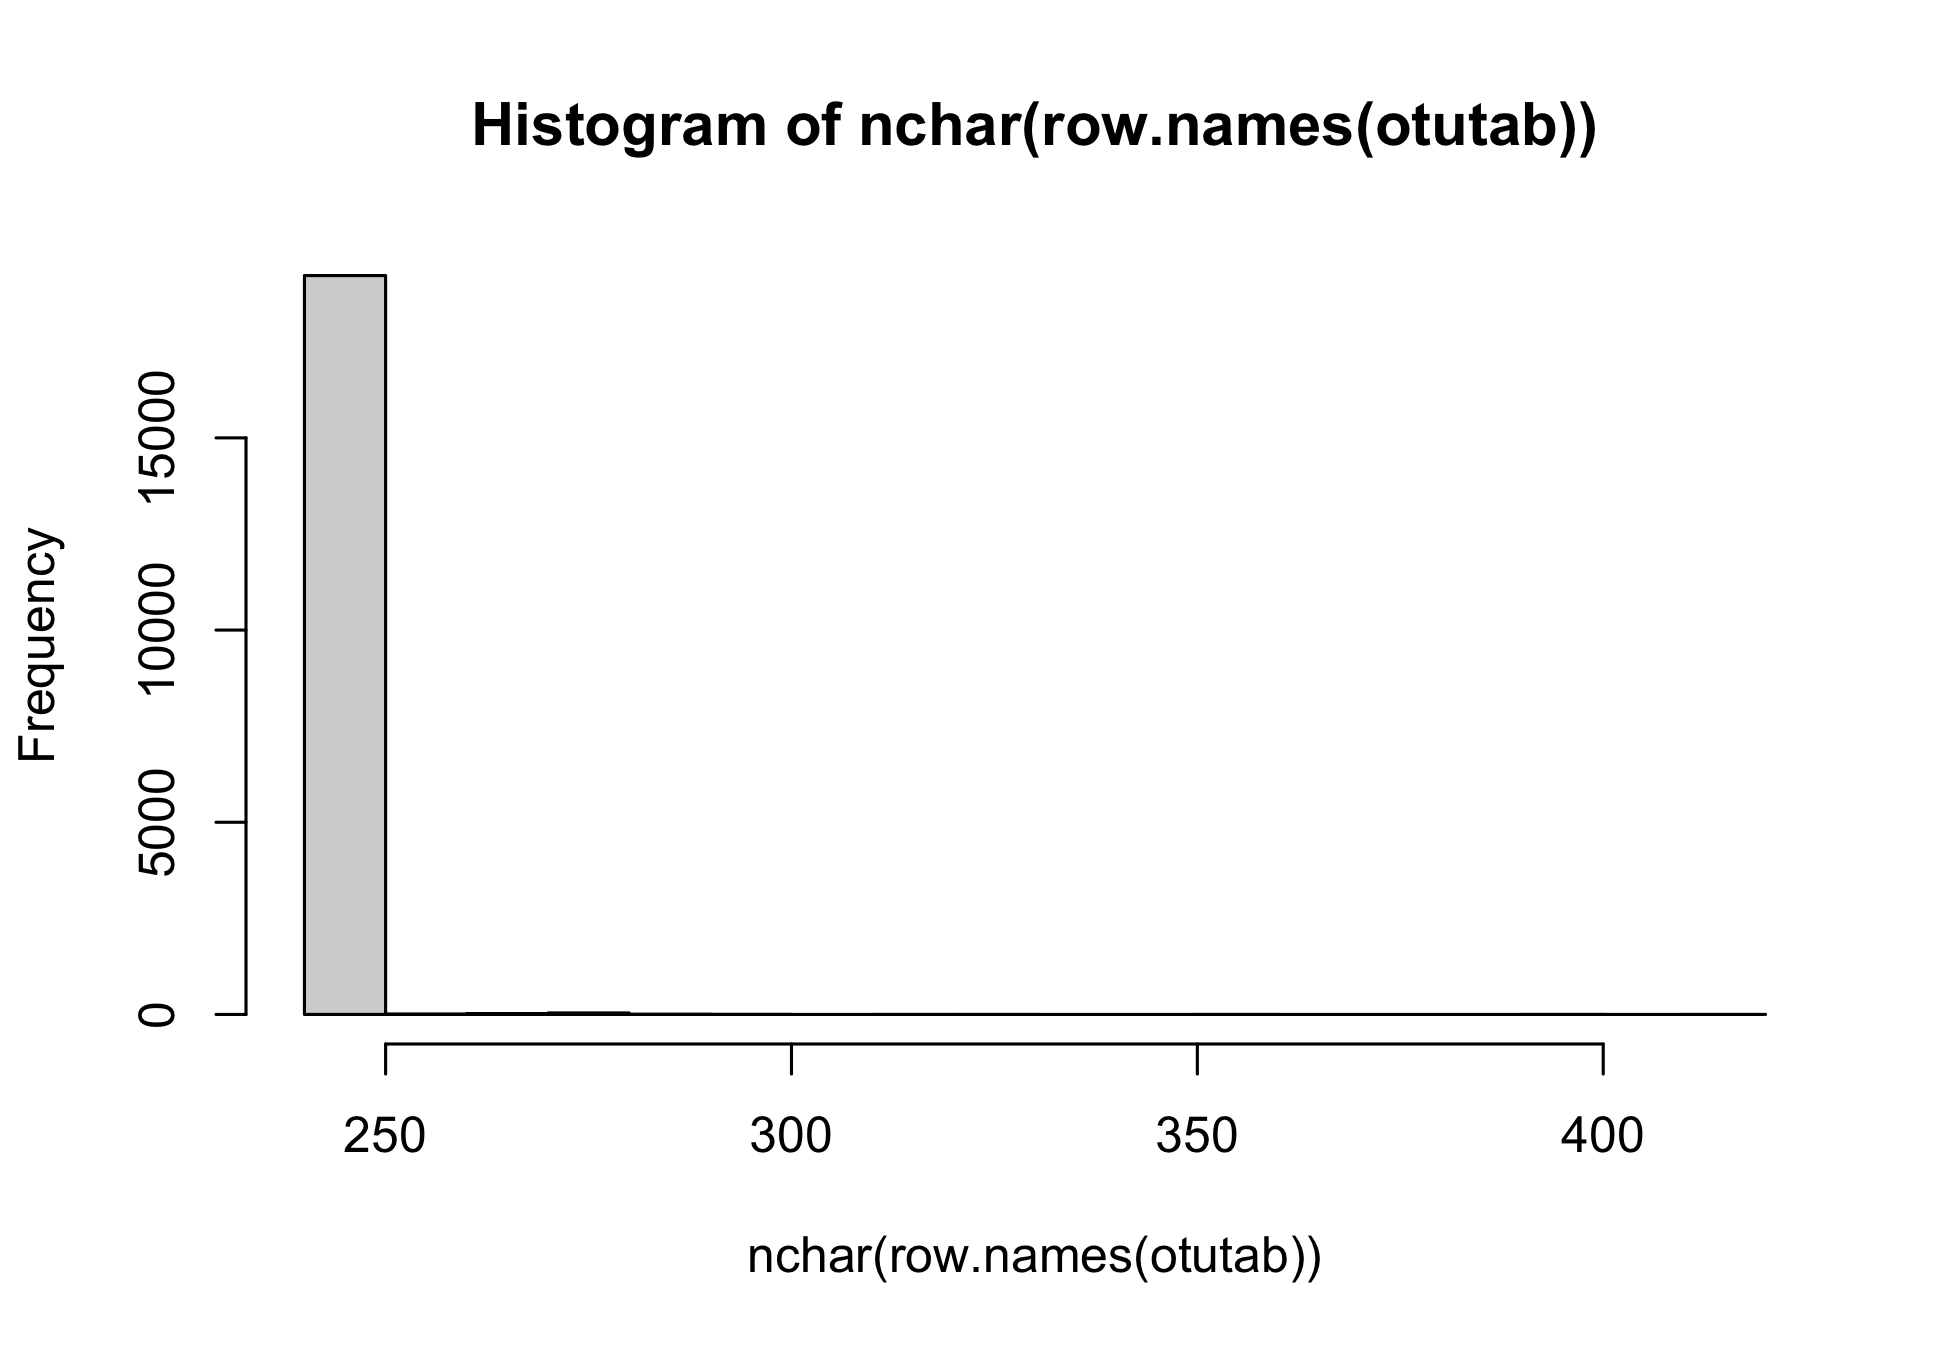
\includegraphics{output-rmd/load-biom-1.png}

\begin{Shaded}
\begin{Highlighting}[]
\KeywordTok{colnames}\NormalTok{(otutab)}
\end{Highlighting}
\end{Shaded}

\begin{verbatim}
##   [1] "001-K1-0-17_S1__F_filt.fastq.gz"         
##   [2] "002-K1-17-45_S2__F_filt.fastq.gz"        
##   [3] "003-K1-45-60_S3__F_filt.fastq.gz"        
##   [4] "004-K2-Muck_S4__F_filt.fastq.gz"         
##   [5] "005-K3-0-15_S5__F_filt.fastq.gz"         
##   [6] "006-K3-15-35_S6__F_filt.fastq.gz"        
##   [7] "007-K3-35-50_S7__F_filt.fastq.gz"        
##   [8] "008-K4-0-15_S8__F_filt.fastq.gz"         
##   [9] "009-K4-15-30_S9__F_filt.fastq.gz"        
##  [10] "010-K4-30-50_S10__F_filt.fastq.gz"       
##  [11] "011-R1-0-27_S11__F_filt.fastq.gz"        
##  [12] "012-R1-27-50_S12__F_filt.fastq.gz"       
##  [13] "013-R1-50-70_S13__F_filt.fastq.gz"       
##  [14] "014-R2-0-30_S14__F_filt.fastq.gz"        
##  [15] "015-R2-30-45_S15__F_filt.fastq.gz"       
##  [16] "016-R2-45-60_S16__F_filt.fastq.gz"       
##  [17] "017-R2-60-100_S17__F_filt.fastq.gz"      
##  [18] "018-R3-0-20_S18__F_filt.fastq.gz"        
##  [19] "019-R3-20-30_S19__F_filt.fastq.gz"       
##  [20] "020-M1-0-31_S20__F_filt.fastq.gz"        
##  [21] "021-M1-31-50_S21__F_filt.fastq.gz"       
##  [22] "022-M1-50-70_S22__F_filt.fastq.gz"       
##  [23] "023-M2-0-24_S23__F_filt.fastq.gz"        
##  [24] "024-M2-24-38_S24__F_filt.fastq.gz"       
##  [25] "025-M2-38-55_S25__F_filt.fastq.gz"       
##  [26] "026-M3-0-15_S26__F_filt.fastq.gz"        
##  [27] "027-M3-15-30_S27__F_filt.fastq.gz"       
##  [28] "028-S-0-30_S28__F_filt.fastq.gz"         
##  [29] "029-S-30-60_S29__F_filt.fastq.gz"        
##  [30] "030-H1-0-30_S30__F_filt.fastq.gz"        
##  [31] "031-H1-30-40_S31__F_filt.fastq.gz"       
##  [32] "032-H1-40-60_S32__F_filt.fastq.gz"       
##  [33] "033-H2-0-30_S33__F_filt.fastq.gz"        
##  [34] "034-H2-30-60_S34__F_filt.fastq.gz"       
##  [35] "035-A249-0-35_S35__F_filt.fastq.gz"      
##  [36] "036-A249-35-60_S36__F_filt.fastq.gz"     
##  [37] "037-A341-0-33_S37__F_filt.fastq.gz"      
##  [38] "038-A341-33-55_S38__F_filt.fastq.gz"     
##  [39] "039-A341-55-75_S39__F_filt.fastq.gz"     
##  [40] "040-A341-75-85_S40__F_filt.fastq.gz"     
##  [41] "041-L2-0-23_S41__F_filt.fastq.gz"        
##  [42] "042-L2-23-45_S42__F_filt.fastq.gz"       
##  [43] "043-L3-0-12_S43__F_filt.fastq.gz"        
##  [44] "044-L3-12-20_S44__F_filt.fastq.gz"       
##  [45] "045-L3-20-40_S45__F_filt.fastq.gz"       
##  [46] "046-L4-0-10_S46__F_filt.fastq.gz"        
##  [47] "047-L4-10-20_S47__F_filt.fastq.gz"       
##  [48] "048-L4-20-40_S48__F_filt.fastq.gz"       
##  [49] "049-W3-Compost_S49__F_filt.fastq.gz"     
##  [50] "050-W4-0-28_S50__F_filt.fastq.gz"        
##  [51] "051-W4-28-45_S51__F_filt.fastq.gz"       
##  [52] "052-W4-45-55_S52__F_filt.fastq.gz"       
##  [53] "053-W5-0-35_S53__F_filt.fastq.gz"        
##  [54] "054-W5-35-65_S54__F_filt.fastq.gz"       
##  [55] "055-W7-0-15_S55__F_filt.fastq.gz"        
##  [56] "056-W7-15-30_S56__F_filt.fastq.gz"       
##  [57] "057-P1-0-30_S57__F_filt.fastq.gz"        
##  [58] "058-P1-30-45_S58__F_filt.fastq.gz"       
##  [59] "059-P1-45-55_S59__F_filt.fastq.gz"       
##  [60] "060-P2-0-20_S60__F_filt.fastq.gz"        
##  [61] "061-P2-20-45_S61__F_filt.fastq.gz"       
##  [62] "062-P2-45-55_S62__F_filt.fastq.gz"       
##  [63] "063-P4-0-25_S63__F_filt.fastq.gz"        
##  [64] "064-P4-25-35_S64__F_filt.fastq.gz"       
##  [65] "065-P4-35-50_S65__F_filt.fastq.gz"       
##  [66] "181-Sp11-Cr31-0-20_S66__F_filt.fastq.gz" 
##  [67] "182-Sp11-Cr32-0-16_S67__F_filt.fastq.gz" 
##  [68] "183-Sp11-Cr33-0-20_S68__F_filt.fastq.gz" 
##  [69] "184-Sp12-Cr34-0-16_S69__F_filt.fastq.gz" 
##  [70] "185-Sp12-Cr35-0-18_S70__F_filt.fastq.gz" 
##  [71] "186-Sp12-Cr36-0-20_S71__F_filt.fastq.gz" 
##  [72] "187-Sp13-Cr37-0-20_S72__F_filt.fastq.gz" 
##  [73] "188-Sp13-Cr38-0-20_S73__F_filt.fastq.gz" 
##  [74] "189-Sp13-Cr39-0-19_S74__F_filt.fastq.gz" 
##  [75] "190-Sp14-Cr40-0-17_S75__F_filt.fastq.gz" 
##  [76] "191-Sp14-Cr41-0-18_S76__F_filt.fastq.gz" 
##  [77] "192-Sp14-Cr42-0-20_S77__F_filt.fastq.gz" 
##  [78] "193-Sp15-Cr43-0-18_S78__F_filt.fastq.gz" 
##  [79] "194-Sp15-Cr44-0-17_S79__F_filt.fastq.gz" 
##  [80] "195-Sp15-Cr45-0-20_S80__F_filt.fastq.gz" 
##  [81] "196-Sp16-Cr46-0-20_S81__F_filt.fastq.gz" 
##  [82] "197-Sp16-Cr47-0-17_S82__F_filt.fastq.gz" 
##  [83] "198-Sp16-Cr48-0-20_S83__F_filt.fastq.gz" 
##  [84] "199-Sp17-Cr49-0-20_S84__F_filt.fastq.gz" 
##  [85] "200-Sp17-Cr50-0-18_S85__F_filt.fastq.gz" 
##  [86] "201-Sp17-Cr51-0-18_S86__F_filt.fastq.gz" 
##  [87] "202-Sp18-Cr52-0-18_S87__F_filt.fastq.gz" 
##  [88] "203-Sp18-Cr53-0-19_S88__F_filt.fastq.gz" 
##  [89] "204-Sp18-Cr54-0-20_S89__F_filt.fastq.gz" 
##  [90] "205-Sp19-Cr55-0-20_S90__F_filt.fastq.gz" 
##  [91] "206-Sp19-Cr56-0-18_S91__F_filt.fastq.gz" 
##  [92] "207-Sp19-Cr57-0-18_S92__F_filt.fastq.gz" 
##  [93] "208-Sp20-Cr58-0-20_S93__F_filt.fastq.gz" 
##  [94] "209-Sp20-Cr59-0-19_S94__F_filt.fastq.gz" 
##  [95] "210-Sp20-Cr60-0-20_S95__F_filt.fastq.gz" 
##  [96] "211-Sp1-Cr1-0-20_S96__F_filt.fastq.gz"   
##  [97] "212-Sp1-Cr2-0-20_S97__F_filt.fastq.gz"   
##  [98] "213-Sp1-Cr3-0-20_S98__F_filt.fastq.gz"   
##  [99] "214-Sp2-Cr4-0-20_S99__F_filt.fastq.gz"   
## [100] "215-Sp2-Cr5-0-20_S100__F_filt.fastq.gz"  
## [101] "216-Sp2-Cr6-0-20_S101__F_filt.fastq.gz"  
## [102] "217-Sp3-Cr7-0-20_S102__F_filt.fastq.gz"  
## [103] "218-Sp3-Cr8-0-20_S103__F_filt.fastq.gz"  
## [104] "219-Sp3-Cr9-0-20_S104__F_filt.fastq.gz"  
## [105] "220-Sp4-Cr10-0-20_S105__F_filt.fastq.gz" 
## [106] "221-Sp4-Cr11-0-20_S106__F_filt.fastq.gz" 
## [107] "222-Sp4-Cr12-0-20_S107__F_filt.fastq.gz" 
## [108] "223-Sp5-Cr13-0-20_S108__F_filt.fastq.gz" 
## [109] "224-Sp5-Cr14-0-20_S109__F_filt.fastq.gz" 
## [110] "225-Sp5-Cr15-0-20_S110__F_filt.fastq.gz" 
## [111] "226-Sp6-Cr16-0-15_S111__F_filt.fastq.gz" 
## [112] "227-Sp6-Cr17-0-20_S112__F_filt.fastq.gz" 
## [113] "228-Sp6-Cr18-0-20_S113__F_filt.fastq.gz" 
## [114] "229-Sp7-Cr19-0-20_S114__F_filt.fastq.gz" 
## [115] "230-Sp7-Cr20-0-20_S115__F_filt.fastq.gz" 
## [116] "231-Sp7-Cr21-0-13_S116__F_filt.fastq.gz" 
## [117] "232-Sp8-Cr22-0-20_S117__F_filt.fastq.gz" 
## [118] "233-Sp8-Cr23-0-20_S118__F_filt.fastq.gz" 
## [119] "234-Sp8-Cr24-0-20_S119__F_filt.fastq.gz" 
## [120] "235-Sp9-Cr25-0-15_S120__F_filt.fastq.gz" 
## [121] "236-Sp9-Cr26-0-20_S121__F_filt.fastq.gz" 
## [122] "237-Sp9-Cr27-0-15_S122__F_filt.fastq.gz" 
## [123] "238-Sp10-Cr28-0-20_S123__F_filt.fastq.gz"
## [124] "239-Sp10-Cr29-0-15_S124__F_filt.fastq.gz"
## [125] "240-Sp10-Cr30-0-20_S125__F_filt.fastq.gz"
## [126] "241-S-0-30-Dry_S126__F_filt.fastq.gz"
\end{verbatim}

\begin{Shaded}
\begin{Highlighting}[]
\CommentTok{# The sample names have suffixes appended to them - we just want sample IDs}
\CommentTok{# Get names}
\NormalTok{names =}\StringTok{ }\KeywordTok{colnames}\NormalTok{(otutab)}
\CommentTok{# Remove last 17 characters}
\NormalTok{newnames =}\StringTok{ }\KeywordTok{gsub}\NormalTok{(}\StringTok{'.\{17\}$'}\NormalTok{, }\StringTok{''}\NormalTok{, names)}
\CommentTok{# Check out names}
\NormalTok{newnames}
\end{Highlighting}
\end{Shaded}

\begin{verbatim}
##   [1] "001-K1-0-17_S1"          "002-K1-17-45_S2"        
##   [3] "003-K1-45-60_S3"         "004-K2-Muck_S4"         
##   [5] "005-K3-0-15_S5"          "006-K3-15-35_S6"        
##   [7] "007-K3-35-50_S7"         "008-K4-0-15_S8"         
##   [9] "009-K4-15-30_S9"         "010-K4-30-50_S10"       
##  [11] "011-R1-0-27_S11"         "012-R1-27-50_S12"       
##  [13] "013-R1-50-70_S13"        "014-R2-0-30_S14"        
##  [15] "015-R2-30-45_S15"        "016-R2-45-60_S16"       
##  [17] "017-R2-60-100_S17"       "018-R3-0-20_S18"        
##  [19] "019-R3-20-30_S19"        "020-M1-0-31_S20"        
##  [21] "021-M1-31-50_S21"        "022-M1-50-70_S22"       
##  [23] "023-M2-0-24_S23"         "024-M2-24-38_S24"       
##  [25] "025-M2-38-55_S25"        "026-M3-0-15_S26"        
##  [27] "027-M3-15-30_S27"        "028-S-0-30_S28"         
##  [29] "029-S-30-60_S29"         "030-H1-0-30_S30"        
##  [31] "031-H1-30-40_S31"        "032-H1-40-60_S32"       
##  [33] "033-H2-0-30_S33"         "034-H2-30-60_S34"       
##  [35] "035-A249-0-35_S35"       "036-A249-35-60_S36"     
##  [37] "037-A341-0-33_S37"       "038-A341-33-55_S38"     
##  [39] "039-A341-55-75_S39"      "040-A341-75-85_S40"     
##  [41] "041-L2-0-23_S41"         "042-L2-23-45_S42"       
##  [43] "043-L3-0-12_S43"         "044-L3-12-20_S44"       
##  [45] "045-L3-20-40_S45"        "046-L4-0-10_S46"        
##  [47] "047-L4-10-20_S47"        "048-L4-20-40_S48"       
##  [49] "049-W3-Compost_S49"      "050-W4-0-28_S50"        
##  [51] "051-W4-28-45_S51"        "052-W4-45-55_S52"       
##  [53] "053-W5-0-35_S53"         "054-W5-35-65_S54"       
##  [55] "055-W7-0-15_S55"         "056-W7-15-30_S56"       
##  [57] "057-P1-0-30_S57"         "058-P1-30-45_S58"       
##  [59] "059-P1-45-55_S59"        "060-P2-0-20_S60"        
##  [61] "061-P2-20-45_S61"        "062-P2-45-55_S62"       
##  [63] "063-P4-0-25_S63"         "064-P4-25-35_S64"       
##  [65] "065-P4-35-50_S65"        "181-Sp11-Cr31-0-20_S66" 
##  [67] "182-Sp11-Cr32-0-16_S67"  "183-Sp11-Cr33-0-20_S68" 
##  [69] "184-Sp12-Cr34-0-16_S69"  "185-Sp12-Cr35-0-18_S70" 
##  [71] "186-Sp12-Cr36-0-20_S71"  "187-Sp13-Cr37-0-20_S72" 
##  [73] "188-Sp13-Cr38-0-20_S73"  "189-Sp13-Cr39-0-19_S74" 
##  [75] "190-Sp14-Cr40-0-17_S75"  "191-Sp14-Cr41-0-18_S76" 
##  [77] "192-Sp14-Cr42-0-20_S77"  "193-Sp15-Cr43-0-18_S78" 
##  [79] "194-Sp15-Cr44-0-17_S79"  "195-Sp15-Cr45-0-20_S80" 
##  [81] "196-Sp16-Cr46-0-20_S81"  "197-Sp16-Cr47-0-17_S82" 
##  [83] "198-Sp16-Cr48-0-20_S83"  "199-Sp17-Cr49-0-20_S84" 
##  [85] "200-Sp17-Cr50-0-18_S85"  "201-Sp17-Cr51-0-18_S86" 
##  [87] "202-Sp18-Cr52-0-18_S87"  "203-Sp18-Cr53-0-19_S88" 
##  [89] "204-Sp18-Cr54-0-20_S89"  "205-Sp19-Cr55-0-20_S90" 
##  [91] "206-Sp19-Cr56-0-18_S91"  "207-Sp19-Cr57-0-18_S92" 
##  [93] "208-Sp20-Cr58-0-20_S93"  "209-Sp20-Cr59-0-19_S94" 
##  [95] "210-Sp20-Cr60-0-20_S95"  "211-Sp1-Cr1-0-20_S96"   
##  [97] "212-Sp1-Cr2-0-20_S97"    "213-Sp1-Cr3-0-20_S98"   
##  [99] "214-Sp2-Cr4-0-20_S99"    "215-Sp2-Cr5-0-20_S100"  
## [101] "216-Sp2-Cr6-0-20_S101"   "217-Sp3-Cr7-0-20_S102"  
## [103] "218-Sp3-Cr8-0-20_S103"   "219-Sp3-Cr9-0-20_S104"  
## [105] "220-Sp4-Cr10-0-20_S105"  "221-Sp4-Cr11-0-20_S106" 
## [107] "222-Sp4-Cr12-0-20_S107"  "223-Sp5-Cr13-0-20_S108" 
## [109] "224-Sp5-Cr14-0-20_S109"  "225-Sp5-Cr15-0-20_S110" 
## [111] "226-Sp6-Cr16-0-15_S111"  "227-Sp6-Cr17-0-20_S112" 
## [113] "228-Sp6-Cr18-0-20_S113"  "229-Sp7-Cr19-0-20_S114" 
## [115] "230-Sp7-Cr20-0-20_S115"  "231-Sp7-Cr21-0-13_S116" 
## [117] "232-Sp8-Cr22-0-20_S117"  "233-Sp8-Cr23-0-20_S118" 
## [119] "234-Sp8-Cr24-0-20_S119"  "235-Sp9-Cr25-0-15_S120" 
## [121] "236-Sp9-Cr26-0-20_S121"  "237-Sp9-Cr27-0-15_S122" 
## [123] "238-Sp10-Cr28-0-20_S123" "239-Sp10-Cr29-0-15_S124"
## [125] "240-Sp10-Cr30-0-20_S125" "241-S-0-30-Dry_S126"
\end{verbatim}

\begin{Shaded}
\begin{Highlighting}[]
\CommentTok{# Assign new names to samples}
\KeywordTok{colnames}\NormalTok{(otutab) =}\StringTok{ }\NormalTok{newnames}

\CommentTok{# Same thing if we wanted to simplify OTU names to IDs}
\CommentTok{# Instead of sequences (although that's useful)}
\NormalTok{otunames=}\KeywordTok{row.names}\NormalTok{(otutab)}
\KeywordTok{length}\NormalTok{(otunames)}
\end{Highlighting}
\end{Shaded}

\begin{verbatim}
## [1] 19313
\end{verbatim}

\begin{Shaded}
\begin{Highlighting}[]
\NormalTok{newotunames =}\StringTok{ }\KeywordTok{paste}\NormalTok{(}\StringTok{"OTU"}\NormalTok{,}\KeywordTok{rep}\NormalTok{(}\DecValTok{1}\OperatorTok{:}\KeywordTok{length}\NormalTok{(otunames)),}\DataTypeTok{sep=}\StringTok{""}\NormalTok{)}
\KeywordTok{head}\NormalTok{(newotunames)}
\end{Highlighting}
\end{Shaded}

\begin{verbatim}
## [1] "OTU1" "OTU2" "OTU3" "OTU4" "OTU5" "OTU6"
\end{verbatim}

\begin{Shaded}
\begin{Highlighting}[]
\KeywordTok{row.names}\NormalTok{(otutab) =}\StringTok{ }\NormalTok{newotunames}
\KeywordTok{head}\NormalTok{(otutab)}
\end{Highlighting}
\end{Shaded}

\begin{verbatim}
## OTU Table:          [6 taxa and 126 samples]
##                      taxa are rows
##      001-K1-0-17_S1 002-K1-17-45_S2 003-K1-45-60_S3 004-K2-Muck_S4
## OTU1              0               0              49              0
## OTU2            461             369               0              0
## OTU3            157             522             429              0
## OTU4            482             159               0              0
## OTU5              0               0               0              0
## OTU6            181             247             271              0
##      005-K3-0-15_S5 006-K3-15-35_S6 007-K3-35-50_S7 008-K4-0-15_S8
## OTU1            115               0              25              0
## OTU2            546             509             983              0
## OTU3             64             343             452              0
## OTU4            452             227             313              0
## OTU5              0               0              24              0
## OTU6            269             429            1184              0
##      009-K4-15-30_S9 010-K4-30-50_S10 011-R1-0-27_S11 012-R1-27-50_S12
## OTU1               0                0            1096              635
## OTU2               0              156             205               84
## OTU3             635             1162             184             1659
## OTU4               0               75             262                0
## OTU5               0                0               0                0
## OTU6               0                0               0              198
##      013-R1-50-70_S13 014-R2-0-30_S14 015-R2-30-45_S15 016-R2-45-60_S16
## OTU1              225            1303              730              349
## OTU2                0               0              233                0
## OTU3             1094               0              984              332
## OTU4                0             167               71                0
## OTU5                0             333              193                0
## OTU6                0               0             1665              456
##      017-R2-60-100_S17 018-R3-0-20_S18 019-R3-20-30_S19 020-M1-0-31_S20
## OTU1              1483             426                0             216
## OTU2                 0             211               64             246
## OTU3               838              45             1711               6
## OTU4                 0              87                0             112
## OTU5                 0              72                0             536
## OTU6               555               0               57               0
##      021-M1-31-50_S21 022-M1-50-70_S22 023-M2-0-24_S23 024-M2-24-38_S24
## OTU1               89              128             149                0
## OTU2              298              258             105                0
## OTU3             1691             5550               5               72
## OTU4              108              183              81                0
## OTU5              279               53             329               98
## OTU6                0              248               0                0
##      025-M2-38-55_S25 026-M3-0-15_S26 027-M3-15-30_S27 028-S-0-30_S28
## OTU1               39             115              656             51
## OTU2                0             424              644            436
## OTU3              904              15             1119             80
## OTU4                0             201              119            240
## OTU5               52             547              457              0
## OTU6                0               0              671            144
##      029-S-30-60_S29 030-H1-0-30_S30 031-H1-30-40_S31 032-H1-40-60_S32
## OTU1              71             354              158              129
## OTU2            1128               0              140              902
## OTU3            1042               0                0                0
## OTU4             181              87               17              105
## OTU5               0             999              163               31
## OTU6             574               0              106              704
##      033-H2-0-30_S33 034-H2-30-60_S34 035-A249-0-35_S35 036-A249-35-60_S36
## OTU1              96              287               462                 95
## OTU2             119              497               322                315
## OTU3               0               15                 0                311
## OTU4              60               82               195                149
## OTU5             138               71              1203                173
## OTU6               0              296               405                479
##      037-A341-0-33_S37 038-A341-33-55_S38 039-A341-55-75_S39 040-A341-75-85_S40
## OTU1               305                119                232                 64
## OTU2               157                695                389                220
## OTU3                 0                126               1302               2972
## OTU4                88                  0                133                 43
## OTU5               682                312                443                129
## OTU6                 0                573                681                256
##      041-L2-0-23_S41 042-L2-23-45_S42 043-L3-0-12_S43 044-L3-12-20_S44
## OTU1              77              174               0              130
## OTU2             788             2370             317              830
## OTU3               0              240               0               14
## OTU4             133              269             121              216
## OTU5             272              166             180              561
## OTU6             263              788               0              483
##      045-L3-20-40_S45 046-L4-0-10_S46 047-L4-10-20_S47 048-L4-20-40_S48
## OTU1               71              27                0               56
## OTU2              674            1202             2267              864
## OTU3              614               0               16              343
## OTU4              265             235              314              367
## OTU5              397             186              303              196
## OTU6              606              32              720              522
##      049-W3-Compost_S49 050-W4-0-28_S50 051-W4-28-45_S51 052-W4-45-55_S52
## OTU1                  0               0              970              257
## OTU2                  0             324             1291             1013
## OTU3                  0               0             2177             1017
## OTU4                  0               0              388              222
## OTU5                  0               0              324              477
## OTU6                  0               0             1538              600
##      053-W5-0-35_S53 054-W5-35-65_S54 055-W7-0-15_S55 056-W7-15-30_S56
## OTU1             367               31             180                0
## OTU2             547             1871             978              459
## OTU3              32              117              94              917
## OTU4             212              210             152               66
## OTU5             430               49             198                0
## OTU6             293             1051             795              542
##      057-P1-0-30_S57 058-P1-30-45_S58 059-P1-45-55_S59 060-P2-0-20_S60
## OTU1             665              135              875             486
## OTU2             548                0               71              77
## OTU3               0               28              130               0
## OTU4              91              105               60             157
## OTU5             588                0               80             447
## OTU6               0                0              390               0
##      061-P2-20-45_S61 062-P2-45-55_S62 063-P4-0-25_S63 064-P4-25-35_S64
## OTU1              192              462             160              335
## OTU2              136                0             395              273
## OTU3                0                0               0                0
## OTU4              124              129             154              244
## OTU5                0              159             497              319
## OTU6                0                0               0                0
##      065-P4-35-50_S65 181-Sp11-Cr31-0-20_S66 182-Sp11-Cr32-0-16_S67
## OTU1              211                    307                    195
## OTU2               79                    231                    242
## OTU3                0                      0                      0
## OTU4              158                    124                    157
## OTU5              256                    204                    170
## OTU6                0                      0                      0
##      183-Sp11-Cr33-0-20_S68 184-Sp12-Cr34-0-16_S69 185-Sp12-Cr35-0-18_S70
## OTU1                    785                    975                    685
## OTU2                    151                    267                    240
## OTU3                      0                      0                      0
## OTU4                    204                    275                   2352
## OTU5                     81                    461                    380
## OTU6                      0                      0                      0
##      186-Sp12-Cr36-0-20_S71 187-Sp13-Cr37-0-20_S72 188-Sp13-Cr38-0-20_S73
## OTU1                    744                    423                   1472
## OTU2                    171                    279                    395
## OTU3                      0                      0                     62
## OTU4                    318                    324                    363
## OTU5                    126                    263                     92
## OTU6                      0                      0                    144
##      189-Sp13-Cr39-0-19_S74 190-Sp14-Cr40-0-17_S75 191-Sp14-Cr41-0-18_S76
## OTU1                   1393                    121                    730
## OTU2                    467                      0                    120
## OTU3                     72                     43                    115
## OTU4                    361                    181                    228
## OTU5                    173                      0                      0
## OTU6                    129                      0                      0
##      192-Sp14-Cr42-0-20_S77 193-Sp15-Cr43-0-18_S78 194-Sp15-Cr44-0-17_S79
## OTU1                    635                   1568                   1439
## OTU2                    179                      0                      0
## OTU3                    140                      0                    479
## OTU4                    359                    376                    235
## OTU5                     47                      0                      0
## OTU6                      0                      0                      0
##      195-Sp15-Cr45-0-20_S80 196-Sp16-Cr46-0-20_S81 197-Sp16-Cr47-0-17_S82
## OTU1                   1037                    321                   1055
## OTU2                      0                      0                    348
## OTU3                      0                      0                      0
## OTU4                    688                    175                    348
## OTU5                     50                    138                    323
## OTU6                      0                      0                    141
##      198-Sp16-Cr48-0-20_S83 199-Sp17-Cr49-0-20_S84 200-Sp17-Cr50-0-18_S85
## OTU1                    397                    492                   1223
## OTU2                    192                      0                      0
## OTU3                      0                    281                    101
## OTU4                    516                    166                   1959
## OTU5                    130                      0                     90
## OTU6                      0                      0                      0
##      201-Sp17-Cr51-0-18_S86 202-Sp18-Cr52-0-18_S87 203-Sp18-Cr53-0-19_S88
## OTU1                    482                   1306                    857
## OTU2                      0                    236                    271
## OTU3                     83                      0                      0
## OTU4                    164                    278                    279
## OTU5                      0                    553                    300
## OTU6                      0                    107                      0
##      204-Sp18-Cr54-0-20_S89 205-Sp19-Cr55-0-20_S90 206-Sp19-Cr56-0-18_S91
## OTU1                   1367                   1716                    113
## OTU2                    227                    162                      0
## OTU3                      0                    242                     51
## OTU4                    347                    446                      0
## OTU5                    384                      0                      0
## OTU6                     83                      0                      0
##      207-Sp19-Cr57-0-18_S92 208-Sp20-Cr58-0-20_S93 209-Sp20-Cr59-0-19_S94
## OTU1                   1179                    997                   1546
## OTU2                      0                    314                    323
## OTU3                     41                      0                     70
## OTU4                      0                    341                    711
## OTU5                      0                    315                    408
## OTU6                      0                      0                    256
##      210-Sp20-Cr60-0-20_S95 211-Sp1-Cr1-0-20_S96 212-Sp1-Cr2-0-20_S97
## OTU1                    878                   99                   96
## OTU2                    225                    0                    0
## OTU3                      0                    0                    0
## OTU4                    181                  127                 2578
## OTU5                    204                    0                    0
## OTU6                    194                    0                    0
##      213-Sp1-Cr3-0-20_S98 214-Sp2-Cr4-0-20_S99 215-Sp2-Cr5-0-20_S100
## OTU1                  253                 1054                     0
## OTU2                    0                  228                     0
## OTU3                   50                    0                     0
## OTU4                    0                  153                     0
## OTU5                    0                    0                     0
## OTU6                    0                    0                     0
##      216-Sp2-Cr6-0-20_S101 217-Sp3-Cr7-0-20_S102 218-Sp3-Cr8-0-20_S103
## OTU1                   356                  1342                  1200
## OTU2                   344                   240                   257
## OTU3                   150                     0                     0
## OTU4                   154                   465                   164
## OTU5                     0                   405                   375
## OTU6                   131                    99                   111
##      219-Sp3-Cr9-0-20_S104 220-Sp4-Cr10-0-20_S105 221-Sp4-Cr11-0-20_S106
## OTU1                  1786                    962                    676
## OTU2                   286                    176                    102
## OTU3                     0                      0                      0
## OTU4                   245                    303                    107
## OTU5                   425                    191                     84
## OTU6                   130                    176                      0
##      222-Sp4-Cr12-0-20_S107 223-Sp5-Cr13-0-20_S108 224-Sp5-Cr14-0-20_S109
## OTU1                   1114                    204                   1062
## OTU2                    363                    132                    313
## OTU3                     33                      0                      0
## OTU4                    336                    202                    417
## OTU5                    547                    224                    505
## OTU6                    388                      0                    228
##      225-Sp5-Cr15-0-20_S110 226-Sp6-Cr16-0-15_S111 227-Sp6-Cr17-0-20_S112
## OTU1                    908                    160                    754
## OTU2                    136                      0                    131
## OTU3                      0                      0                      0
## OTU4                    227                    196                    316
## OTU5                    204                    143                    329
## OTU6                      0                      0                     70
##      228-Sp6-Cr18-0-20_S113 229-Sp7-Cr19-0-20_S114 230-Sp7-Cr20-0-20_S115
## OTU1                    377                    296                    300
## OTU2                    233                      0                      0
## OTU3                      0                    250                      0
## OTU4                    172                    235                    250
## OTU5                    330                      0                      0
## OTU6                      0                      0                      0
##      231-Sp7-Cr21-0-13_S116 232-Sp8-Cr22-0-20_S117 233-Sp8-Cr23-0-20_S118
## OTU1                    525                   1144                    831
## OTU2                      0                    469                    484
## OTU3                     44                     93                     97
## OTU4                      0                    415                    280
## OTU5                      0                    183                     84
## OTU6                      0                    129                      0
##      234-Sp8-Cr24-0-20_S119 235-Sp9-Cr25-0-15_S120 236-Sp9-Cr26-0-20_S121
## OTU1                    312                    753                    405
## OTU2                    776                    160                    204
## OTU3                     71                      0                      0
## OTU4                    287                    190                    196
## OTU5                    169                    412                    484
## OTU6                      0                      0                      0
##      237-Sp9-Cr27-0-15_S122 238-Sp10-Cr28-0-20_S123 239-Sp10-Cr29-0-15_S124
## OTU1                    611                     353                     271
## OTU2                    126                       0                       0
## OTU3                      0                     144                      43
## OTU4                     61                     169                     319
## OTU5                    224                      35                      55
## OTU6                      0                       0                       0
##      240-Sp10-Cr30-0-20_S125 241-S-0-30-Dry_S126
## OTU1                     130                   0
## OTU2                       0                 204
## OTU3                      58                 312
## OTU4                     114                 160
## OTU5                       0                   0
## OTU6                       0                   0
\end{verbatim}

\begin{Shaded}
\begin{Highlighting}[]
\CommentTok{# Cut off the sampling ID to match metadata}
\ControlFlowTok{for}\NormalTok{ (i }\ControlFlowTok{in} \DecValTok{1}\OperatorTok{:}\KeywordTok{length}\NormalTok{(}\KeywordTok{colnames}\NormalTok{(otutab)))\{}
\NormalTok{  newname =}\StringTok{ }\KeywordTok{strsplit}\NormalTok{(}\KeywordTok{colnames}\NormalTok{(otutab[i]),}\StringTok{"_"}\NormalTok{)[[i]][}\DecValTok{1}\NormalTok{]}
  \KeywordTok{colnames}\NormalTok{(otutab)[i]=newname}
\NormalTok{\}}

\CommentTok{# Import sample data}
\NormalTok{samdat =}\StringTok{ }\KeywordTok{read.csv}\NormalTok{(}\StringTok{"source/metrology-compiled/2020-03-12-hatch-data-merged-as-metadata.csv"}\NormalTok{, }\DataTypeTok{header=}\NormalTok{T)}
\CommentTok{# samdat$Sample.ID = as.character(samdat$Sample.ID)}
\CommentTok{# samdat$Sample.ID[1:9] = paste("00",samdat$Sample.ID[1:9],sep="")}
\CommentTok{# samdat$Sample.ID[10:length(samdat$Sample.ID)] = paste("0",samdat$Sample.ID[10:length(samdat$Sample.ID)],sep="")}

\CommentTok{# Check we have all the same sample names now}
\NormalTok{samdat}\OperatorTok{$}\NormalTok{Sample.ID[}\DecValTok{1}\OperatorTok{:}\DecValTok{65}\NormalTok{] }\OperatorTok{==}\StringTok{ }\KeywordTok{colnames}\NormalTok{(otutab)[}\DecValTok{1}\OperatorTok{:}\DecValTok{65}\NormalTok{]}
\end{Highlighting}
\end{Shaded}

\begin{verbatim}
##  [1] TRUE TRUE TRUE TRUE TRUE TRUE TRUE TRUE TRUE TRUE TRUE TRUE TRUE TRUE TRUE
## [16] TRUE TRUE TRUE TRUE TRUE TRUE TRUE TRUE TRUE TRUE TRUE TRUE TRUE TRUE TRUE
## [31] TRUE TRUE TRUE TRUE TRUE TRUE TRUE TRUE TRUE TRUE TRUE TRUE TRUE TRUE TRUE
## [46] TRUE TRUE TRUE TRUE TRUE TRUE TRUE TRUE TRUE TRUE TRUE TRUE TRUE TRUE TRUE
## [61] TRUE TRUE TRUE TRUE TRUE
\end{verbatim}

\begin{Shaded}
\begin{Highlighting}[]
\NormalTok{samdat}\OperatorTok{$}\NormalTok{Sample.ID[}\DecValTok{66}\OperatorTok{:}\DecValTok{125}\NormalTok{] }\OperatorTok{==}\StringTok{ }\KeywordTok{colnames}\NormalTok{(otutab)[}\DecValTok{66}\OperatorTok{:}\DecValTok{125}\NormalTok{]}
\end{Highlighting}
\end{Shaded}

\begin{verbatim}
##  [1] TRUE TRUE TRUE TRUE TRUE TRUE TRUE TRUE TRUE TRUE TRUE TRUE TRUE TRUE TRUE
## [16] TRUE TRUE TRUE TRUE TRUE TRUE TRUE TRUE TRUE TRUE TRUE TRUE TRUE TRUE TRUE
## [31] TRUE TRUE TRUE TRUE TRUE TRUE TRUE TRUE TRUE TRUE TRUE TRUE TRUE TRUE TRUE
## [46] TRUE TRUE TRUE TRUE TRUE TRUE TRUE TRUE TRUE TRUE TRUE TRUE TRUE TRUE TRUE
\end{verbatim}

\begin{Shaded}
\begin{Highlighting}[]
\NormalTok{samdat =}\StringTok{ }\KeywordTok{sample_data}\NormalTok{(samdat)}

\CommentTok{# Exponentiate all pH values}
\NormalTok{samdat}\OperatorTok{$}\NormalTok{DNA.Extr.Hplus.After.C1 <-}\StringTok{ }\DecValTok{10}\OperatorTok{^-}\NormalTok{samdat}\OperatorTok{$}\NormalTok{DNA.Extr.pH.After.C1}
\NormalTok{samdat}\OperatorTok{$}\NormalTok{DNA.Extr.Hplus.After.C2 <-}\StringTok{ }\DecValTok{10}\OperatorTok{^-}\NormalTok{samdat}\OperatorTok{$}\NormalTok{DNA.Extr.pH.After.C2}
\NormalTok{samdat}\OperatorTok{$}\NormalTok{Lab.CO2.Hplus.one2one <-}\StringTok{ }\DecValTok{10}\OperatorTok{^-}\NormalTok{samdat}\OperatorTok{$}\NormalTok{Lab.CO2.pH.one2one}
\NormalTok{samdat}\OperatorTok{$}\NormalTok{Lab.CO2.Hplus.one2two <-}\StringTok{ }\DecValTok{10}\OperatorTok{^-}\NormalTok{samdat}\OperatorTok{$}\NormalTok{Lab.CO2.pH.one2two}
\NormalTok{samdat}\OperatorTok{$}\NormalTok{Lab.CO2.Hplus.one2three <-}\StringTok{ }\DecValTok{10}\OperatorTok{^-}\NormalTok{samdat}\OperatorTok{$}\NormalTok{Lab.CO2.pH.one2three}
\NormalTok{samdat}\OperatorTok{$}\NormalTok{Lab.CO2.Hplus.one2four <-}\StringTok{ }\DecValTok{10}\OperatorTok{^-}\NormalTok{samdat}\OperatorTok{$}\NormalTok{Lab.CO2.pH.one2four}
\NormalTok{samdat}\OperatorTok{$}\NormalTok{High.CO2.Hplus.one2one <-}\StringTok{ }\DecValTok{10}\OperatorTok{^-}\NormalTok{samdat}\OperatorTok{$}\NormalTok{High.CO2.pH.one2one}
\NormalTok{samdat}\OperatorTok{$}\NormalTok{High.CO2.Hplus.one2two <-}\StringTok{ }\DecValTok{10}\OperatorTok{^-}\NormalTok{samdat}\OperatorTok{$}\NormalTok{High.CO2.pH.one2two}
\NormalTok{samdat}\OperatorTok{$}\NormalTok{High.CO2.Hplus.one2three <-}\StringTok{ }\DecValTok{10}\OperatorTok{^-}\NormalTok{samdat}\OperatorTok{$}\NormalTok{High.CO2.pH.one2three}
\NormalTok{samdat}\OperatorTok{$}\NormalTok{High.CO2.Hplus.one2four <-}\StringTok{ }\DecValTok{10}\OperatorTok{^-}\NormalTok{samdat}\OperatorTok{$}\NormalTok{High.CO2.pH.one2four}

\KeywordTok{row.names}\NormalTok{(samdat) =}\StringTok{ }\NormalTok{samdat}\OperatorTok{$}\NormalTok{Sample.ID}

\CommentTok{# Create phyloseq object}
\NormalTok{ps =}\StringTok{ }\KeywordTok{phyloseq}\NormalTok{(}\DataTypeTok{otu_table=}\NormalTok{otutab,}\DataTypeTok{sample_data=}\NormalTok{samdat)}
\NormalTok{ps =}\StringTok{ }\KeywordTok{subset_samples}\NormalTok{(ps, Sample.ID }\OperatorTok{!=}\StringTok{ "049-W3-Compost"} \OperatorTok{&}\StringTok{ }\NormalTok{Sample.ID}\OperatorTok{!=}\StringTok{"004-K2-Muck"} \OperatorTok{&}\StringTok{ }\NormalTok{Sample.ID}\OperatorTok{!=}\StringTok{"028-S-0-30"} \OperatorTok{&}\StringTok{ }\NormalTok{Sample.ID}\OperatorTok{!=}\StringTok{"029-S-30-60"}\NormalTok{)}
\end{Highlighting}
\end{Shaded}

\begin{Shaded}
\begin{Highlighting}[]
\NormalTok{ps.melt =}\StringTok{ }\KeywordTok{psmelt}\NormalTok{(ps)}
\NormalTok{ps.melt}

\KeywordTok{head}\NormalTok{(ps.melt)}

\KeywordTok{hist}\NormalTok{(}\KeywordTok{sample_sums}\NormalTok{(ps))}
\end{Highlighting}
\end{Shaded}

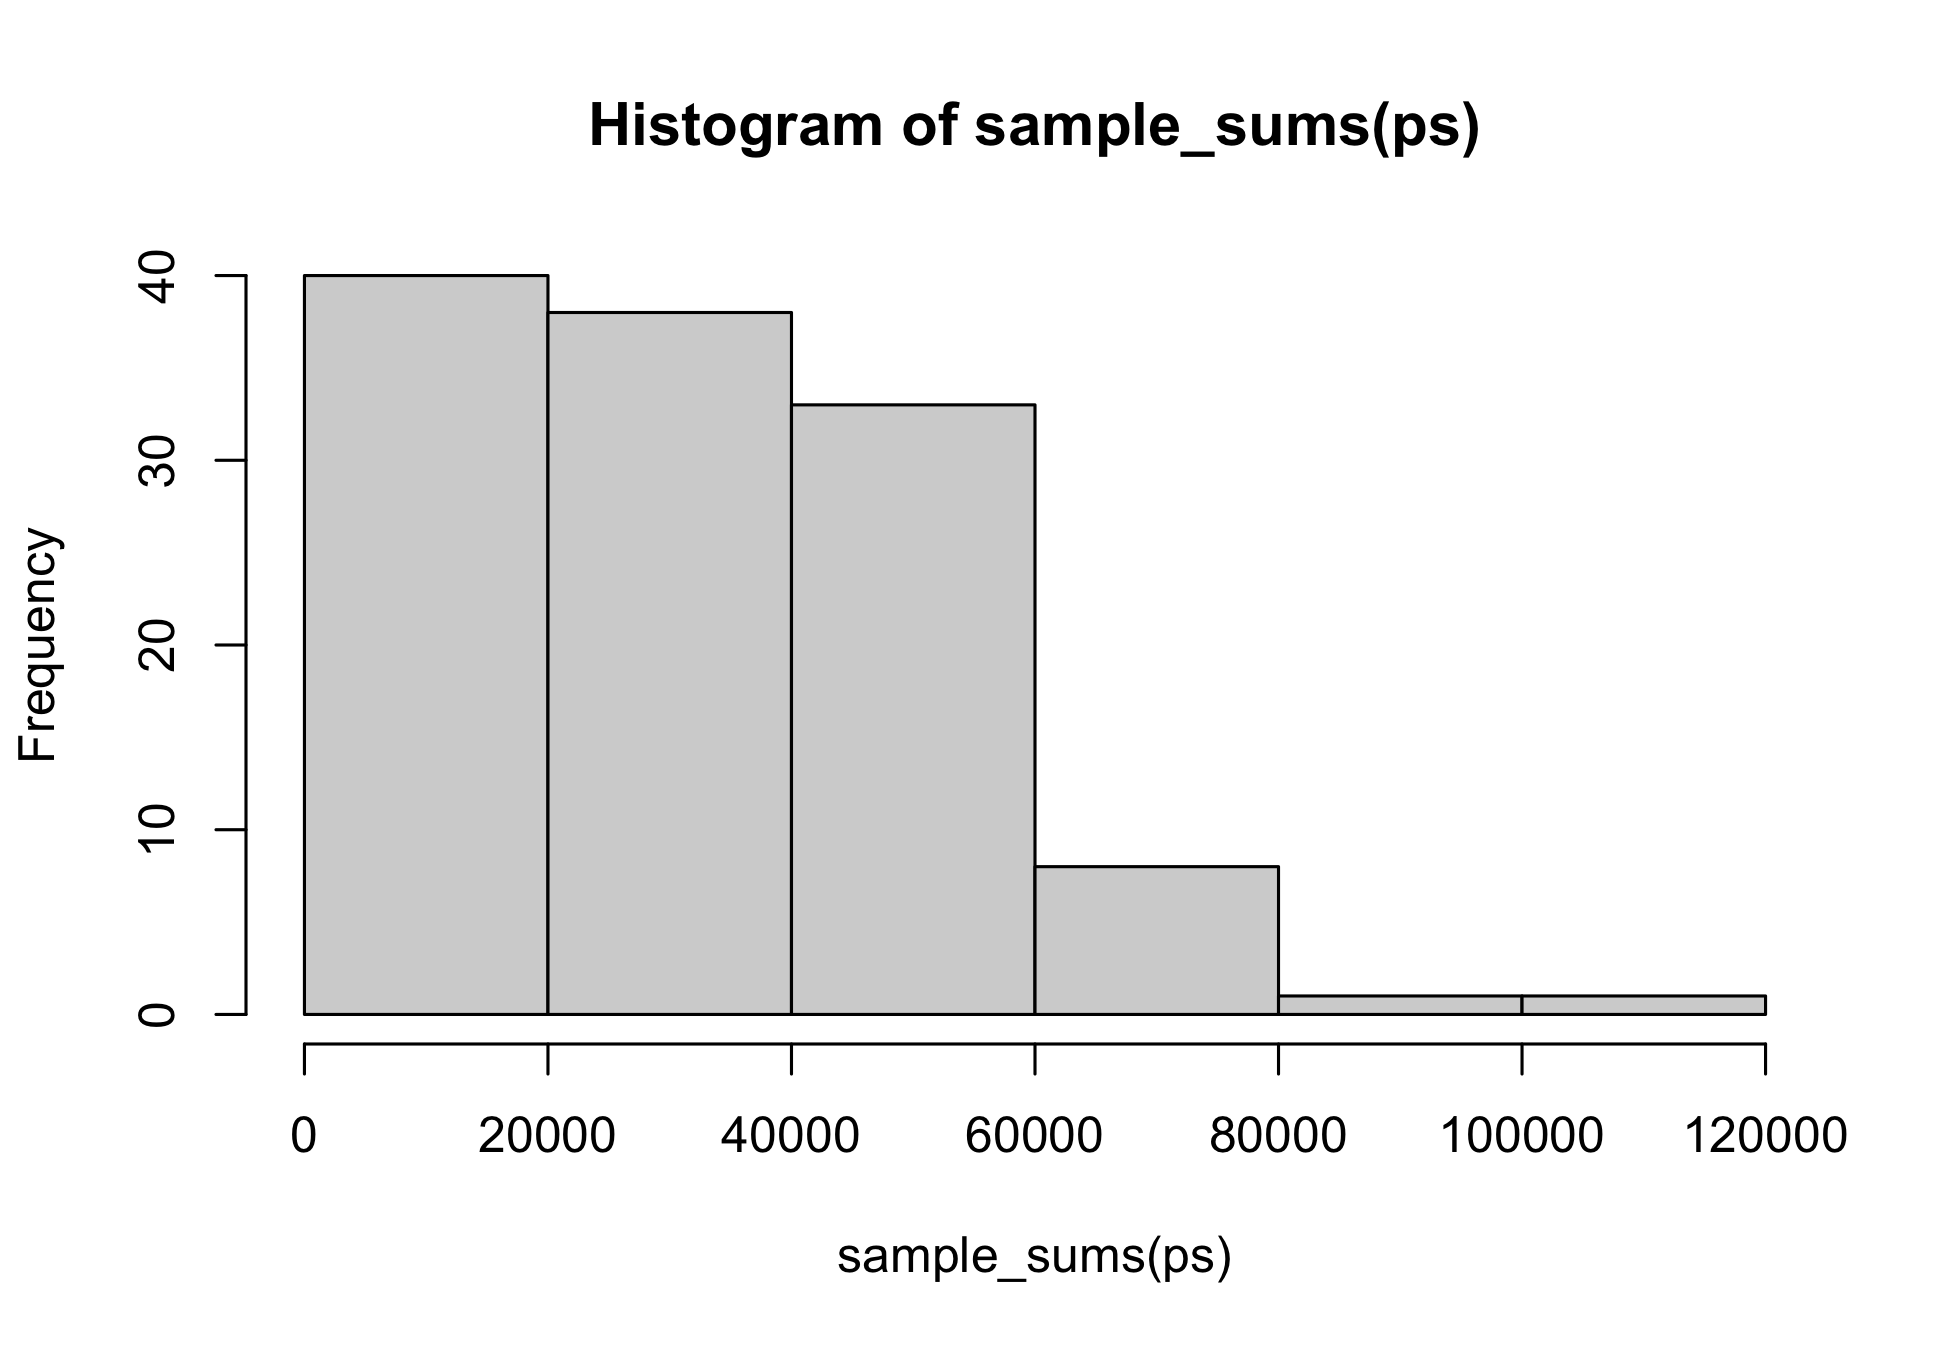
\includegraphics{output-rmd/unnamed-chunk-1-1.png}

\begin{Shaded}
\begin{Highlighting}[]
\CommentTok{# Relative abundances}
\NormalTok{ps.norm =}\StringTok{ }\KeywordTok{transform_sample_counts}\NormalTok{(ps,}\ControlFlowTok{function}\NormalTok{(x) x}\OperatorTok{/}\KeywordTok{sum}\NormalTok{(x))}
\KeywordTok{head}\NormalTok{(}\KeywordTok{otu_table}\NormalTok{(ps.norm))}
\KeywordTok{sample_sums}\NormalTok{(ps.norm)}
\CommentTok{# Looks good}

\KeywordTok{colnames}\NormalTok{(}\KeywordTok{sample_data}\NormalTok{(ps.norm))}
\end{Highlighting}
\end{Shaded}

\hypertarget{acidity-values}{%
\subsection{Acidity Values}\label{acidity-values}}

\hypertarget{diversity-plots}{%
\subsubsection{Diversity Plots}\label{diversity-plots}}

\begin{Shaded}
\begin{Highlighting}[]
\NormalTok{ps.ord.nmds =}\StringTok{ }\KeywordTok{ordinate}\NormalTok{(ps.norm, }\StringTok{"NMDS"}\NormalTok{, }\StringTok{"bray"}\NormalTok{, }\DataTypeTok{trymax=}\DecValTok{1000}\NormalTok{, }\DataTypeTok{k=}\DecValTok{3}\NormalTok{)}
\end{Highlighting}
\end{Shaded}

\begin{verbatim}
## Run 0 stress 0.1077299 
## Run 1 stress 0.1062409 
## ... New best solution
## ... Procrustes: rmse 0.009714332  max resid 0.07846253 
## Run 2 stress 0.1064443 
## ... Procrustes: rmse 0.003447317  max resid 0.02062134 
## Run 3 stress 0.1109859 
## Run 4 stress 0.1107367 
## Run 5 stress 0.1112542 
## Run 6 stress 0.1089057 
## Run 7 stress 0.1088437 
## Run 8 stress 0.1114757 
## Run 9 stress 0.1077522 
## Run 10 stress 0.10623 
## ... New best solution
## ... Procrustes: rmse 0.000980044  max resid 0.006106316 
## ... Similar to previous best
## Run 11 stress 0.1080661 
## Run 12 stress 0.1099741 
## Run 13 stress 0.1106391 
## Run 14 stress 0.1105539 
## Run 15 stress 0.1062336 
## ... Procrustes: rmse 0.0008791491  max resid 0.005394994 
## ... Similar to previous best
## Run 16 stress 0.1107269 
## Run 17 stress 0.1140442 
## Run 18 stress 0.1069135 
## Run 19 stress 0.1069105 
## Run 20 stress 0.1106394 
## *** Solution reached
\end{verbatim}

\begin{Shaded}
\begin{Highlighting}[]
\NormalTok{p =}\StringTok{ }\KeywordTok{plot_ordination}\NormalTok{(ps.norm, ps.ord.nmds, }\DataTypeTok{type=}\StringTok{"samples"}\NormalTok{)}
\NormalTok{palette =}\StringTok{ }\KeywordTok{brewer.pal}\NormalTok{(}\DecValTok{8}\NormalTok{, }\StringTok{"Spectral"}\NormalTok{)}
\NormalTok{p =}\StringTok{ }\NormalTok{p }\OperatorTok{+}\StringTok{ }\KeywordTok{aes}\NormalTok{(}\DataTypeTok{colour=}\NormalTok{Lab.CO2.pH.one2one, }\DataTypeTok{shape=}\NormalTok{Study) }\OperatorTok{+}\StringTok{ }\KeywordTok{geom_point}\NormalTok{(}\DataTypeTok{size=}\DecValTok{3}\NormalTok{) }\OperatorTok{+}\StringTok{ }
\StringTok{  }\KeywordTok{scale_colour_gradientn}\NormalTok{(}\DataTypeTok{colors=}\NormalTok{palette) }\OperatorTok{+}\StringTok{ }
\StringTok{  }\KeywordTok{theme_bw}\NormalTok{()}
\NormalTok{p}
\end{Highlighting}
\end{Shaded}

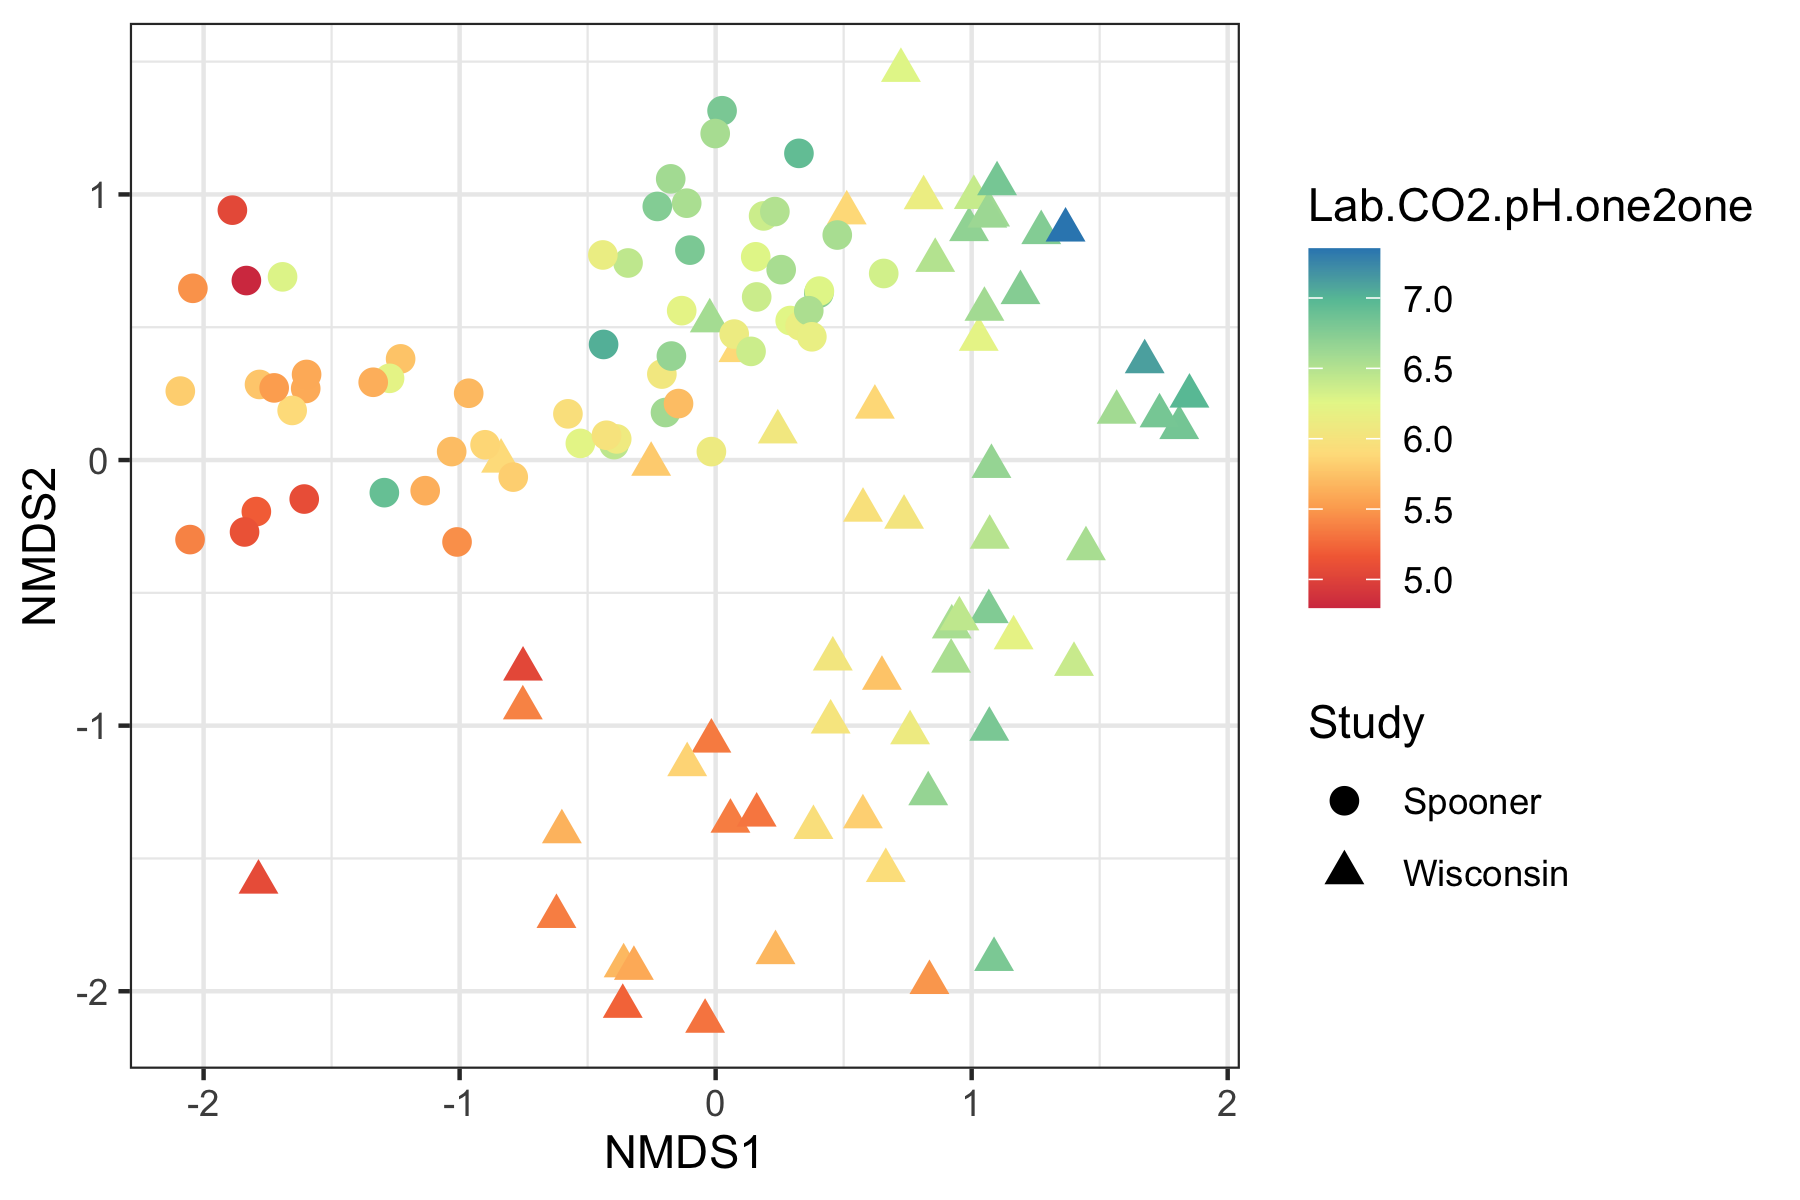
\includegraphics{output-rmd/nmds-bray-soilph-Lab.CO2.pH.one2one-both-studies-1.png}

\begin{Shaded}
\begin{Highlighting}[]
\NormalTok{ps.ord.nmds =}\StringTok{ }\KeywordTok{ordinate}\NormalTok{(ps.norm, }\StringTok{"NMDS"}\NormalTok{, }\StringTok{"bray"}\NormalTok{,}\DataTypeTok{trymax=}\DecValTok{1000}\NormalTok{,}\DataTypeTok{k=}\DecValTok{3}\NormalTok{)}
\end{Highlighting}
\end{Shaded}

\begin{verbatim}
## Run 0 stress 0.1077299 
## Run 1 stress 0.1094413 
## Run 2 stress 0.1090134 
## Run 3 stress 0.1130495 
## Run 4 stress 0.1109678 
## Run 5 stress 0.1089022 
## Run 6 stress 0.1062346 
## ... New best solution
## ... Procrustes: rmse 0.009771967  max resid 0.0785758 
## Run 7 stress 0.1100476 
## Run 8 stress 0.1092704 
## Run 9 stress 0.1092401 
## Run 10 stress 0.1143248 
## Run 11 stress 0.1095969 
## Run 12 stress 0.1110525 
## Run 13 stress 0.1095997 
## Run 14 stress 0.1108272 
## Run 15 stress 0.1088219 
## Run 16 stress 0.1088249 
## Run 17 stress 0.1113368 
## Run 18 stress 0.109001 
## Run 19 stress 0.1105526 
## Run 20 stress 0.1089912 
## Run 21 stress 0.1105958 
## Run 22 stress 0.1085858 
## Run 23 stress 0.1092051 
## Run 24 stress 0.1071714 
## Run 25 stress 0.1097783 
## Run 26 stress 0.1118896 
## Run 27 stress 0.1091024 
## Run 28 stress 0.1092383 
## Run 29 stress 0.1088098 
## Run 30 stress 0.110727 
## Run 31 stress 0.1097888 
## Run 32 stress 0.1092023 
## Run 33 stress 0.1093198 
## Run 34 stress 0.1071659 
## Run 35 stress 0.110058 
## Run 36 stress 0.1081499 
## Run 37 stress 0.1080465 
## Run 38 stress 0.1120458 
## Run 39 stress 0.1112988 
## Run 40 stress 0.1108596 
## Run 41 stress 0.1100633 
## Run 42 stress 0.1120326 
## Run 43 stress 0.1133401 
## Run 44 stress 0.1123775 
## Run 45 stress 0.1109117 
## Run 46 stress 0.1132935 
## Run 47 stress 0.1080668 
## Run 48 stress 0.1107055 
## Run 49 stress 0.1112626 
## Run 50 stress 0.1115894 
## Run 51 stress 0.1073883 
## Run 52 stress 0.109006 
## Run 53 stress 0.1080555 
## Run 54 stress 0.1120686 
## Run 55 stress 0.1166553 
## Run 56 stress 0.1099762 
## Run 57 stress 0.1080678 
## Run 58 stress 0.1087489 
## Run 59 stress 0.1118025 
## Run 60 stress 0.1083055 
## Run 61 stress 0.1120662 
## Run 62 stress 0.1119852 
## Run 63 stress 0.1087742 
## Run 64 stress 0.1085347 
## Run 65 stress 0.1083901 
## Run 66 stress 0.1109853 
## Run 67 stress 0.1110456 
## Run 68 stress 0.1116767 
## Run 69 stress 0.1099292 
## Run 70 stress 0.1073877 
## Run 71 stress 0.1137116 
## Run 72 stress 0.1087757 
## Run 73 stress 0.1076178 
## Run 74 stress 0.1119471 
## Run 75 stress 0.1062314 
## ... New best solution
## ... Procrustes: rmse 0.001088941  max resid 0.008606552 
## ... Similar to previous best
## *** Solution reached
\end{verbatim}

\begin{Shaded}
\begin{Highlighting}[]
\NormalTok{p =}\StringTok{ }\KeywordTok{plot_ordination}\NormalTok{(ps.norm, ps.ord.nmds, }\DataTypeTok{type=}\StringTok{"samples"}\NormalTok{)}
\NormalTok{palette =}\StringTok{ }\KeywordTok{brewer.pal}\NormalTok{(}\DecValTok{8}\NormalTok{, }\StringTok{"Spectral"}\NormalTok{)}
\NormalTok{p =}\StringTok{ }\NormalTok{p }\OperatorTok{+}\StringTok{ }\KeywordTok{aes}\NormalTok{(}\DataTypeTok{colour=}\NormalTok{Lab.CO2.pH.one2one) }\OperatorTok{+}\StringTok{ }\KeywordTok{geom_point}\NormalTok{(}\DataTypeTok{size=}\DecValTok{3}\NormalTok{) }\OperatorTok{+}\StringTok{ }
\StringTok{  }\KeywordTok{scale_colour_gradientn}\NormalTok{(}\DataTypeTok{colors=}\NormalTok{palette) }\OperatorTok{+}\StringTok{ }\KeywordTok{facet_wrap}\NormalTok{(}\OperatorTok{~}\NormalTok{Study) }\OperatorTok{+}\StringTok{ }
\StringTok{  }\KeywordTok{theme_bw}\NormalTok{()}
\NormalTok{p}
\end{Highlighting}
\end{Shaded}

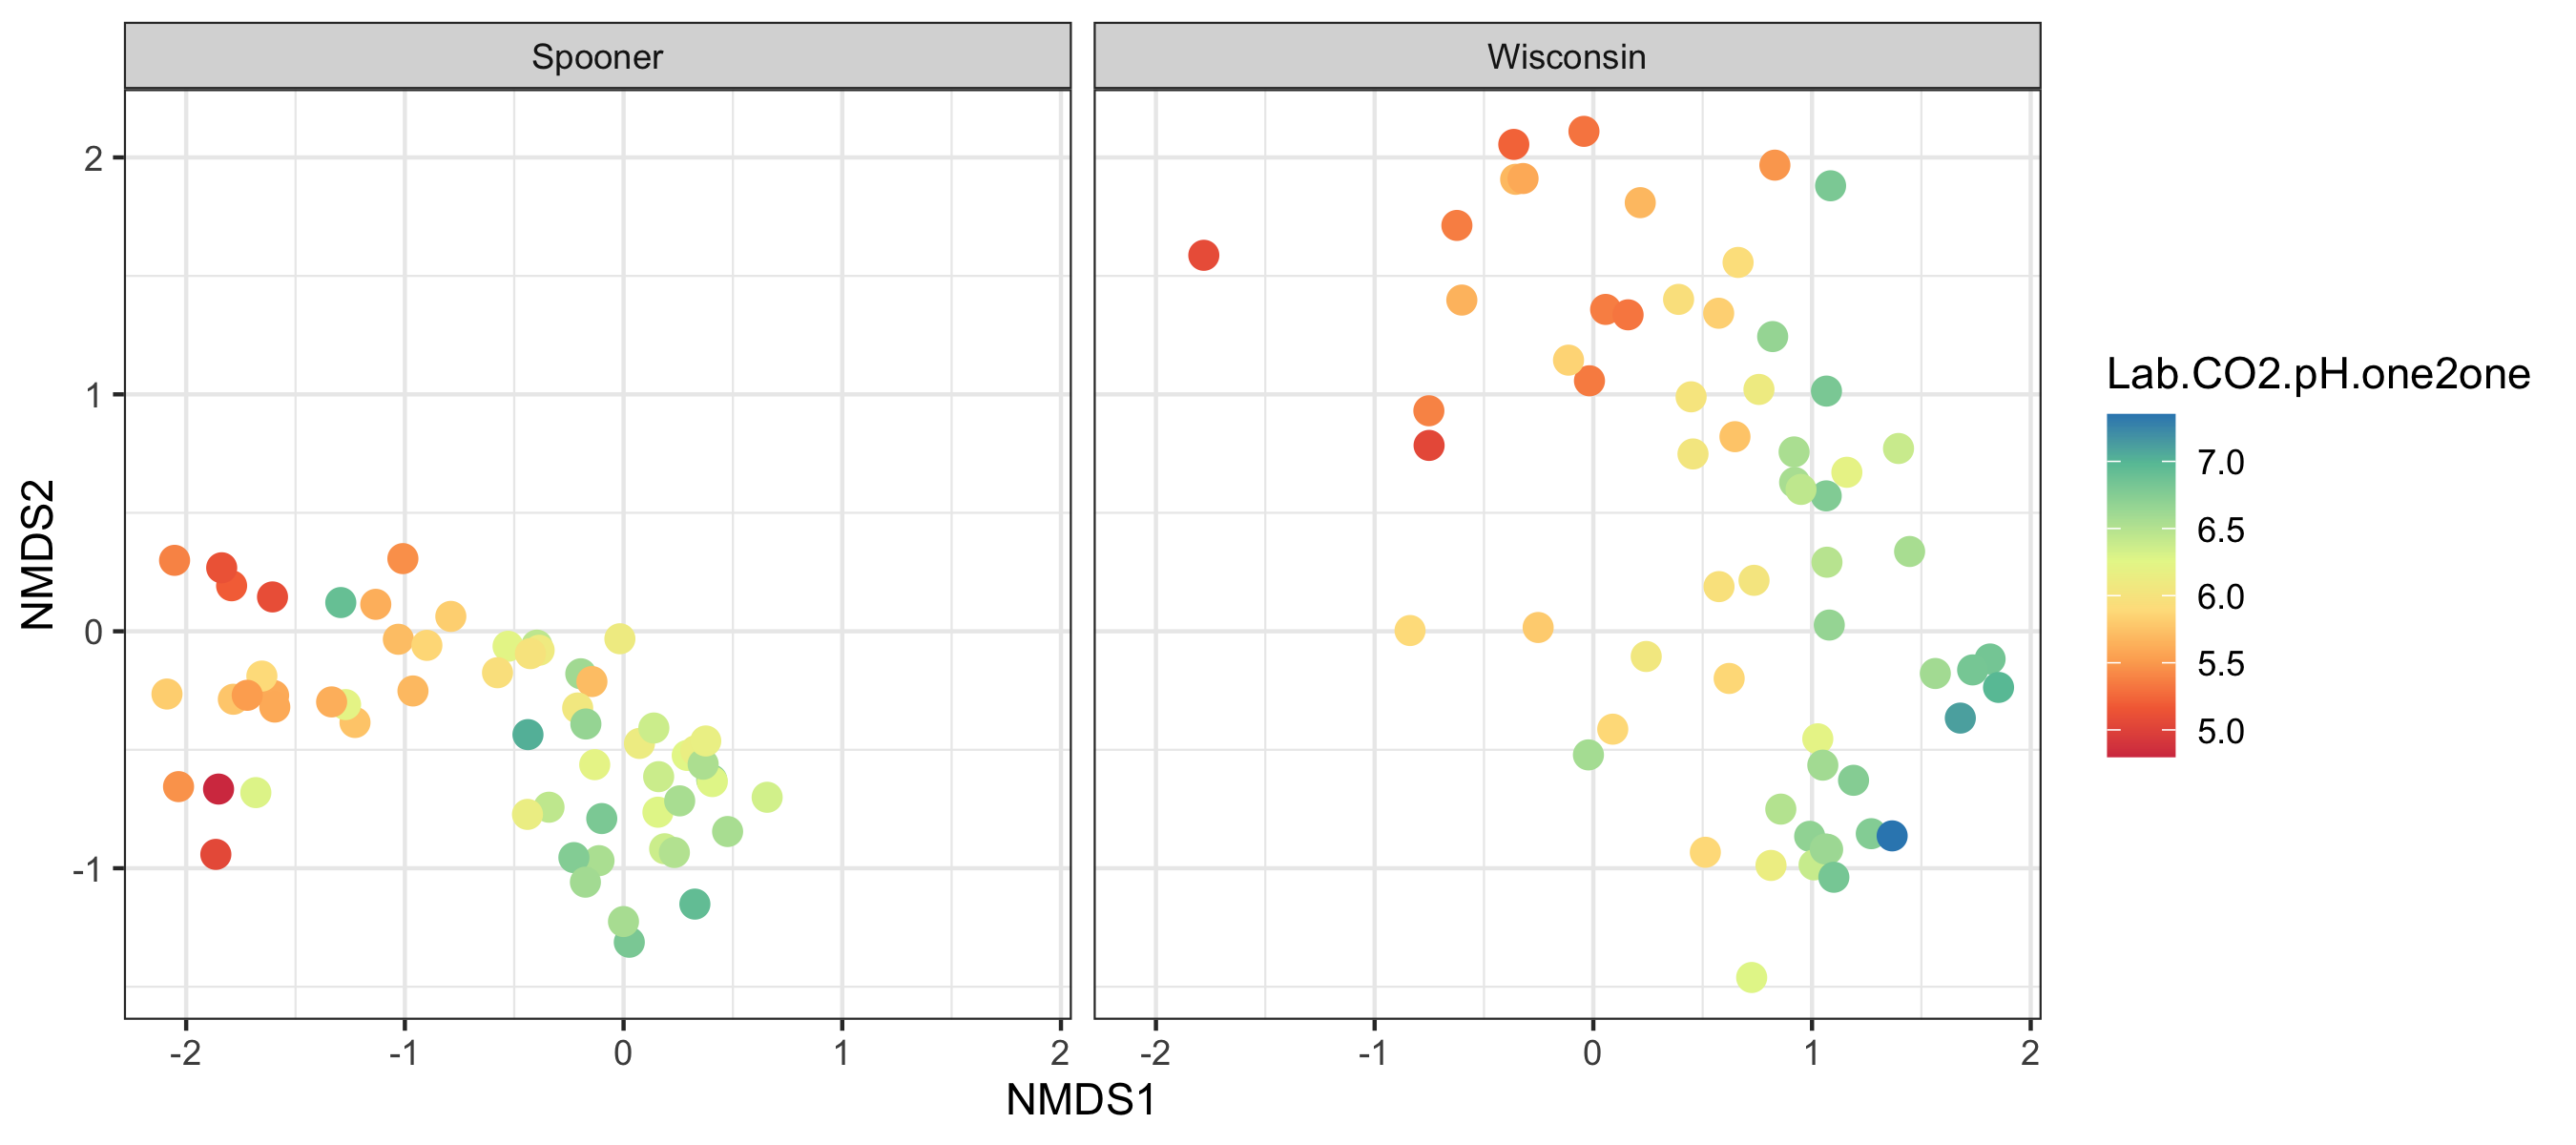
\includegraphics{output-rmd/nmds-bray-soilph-Lab.CO2.pH.one2one-1.png}

\begin{Shaded}
\begin{Highlighting}[]
\NormalTok{ps.ord.nmds =}\StringTok{ }\KeywordTok{ordinate}\NormalTok{(ps.norm, }\StringTok{"NMDS"}\NormalTok{, }\StringTok{"bray"}\NormalTok{,}\DataTypeTok{trymax=}\DecValTok{1000}\NormalTok{,}\DataTypeTok{k=}\DecValTok{3}\NormalTok{)}
\end{Highlighting}
\end{Shaded}

\begin{verbatim}
## Run 0 stress 0.1077299 
## Run 1 stress 0.1125296 
## Run 2 stress 0.108823 
## Run 3 stress 0.1099643 
## Run 4 stress 0.1132349 
## Run 5 stress 0.1138727 
## Run 6 stress 0.1062301 
## ... New best solution
## ... Procrustes: rmse 0.009744973  max resid 0.07842577 
## Run 7 stress 0.1095965 
## Run 8 stress 0.110972 
## Run 9 stress 0.1125236 
## Run 10 stress 0.1109878 
## Run 11 stress 0.1100633 
## Run 12 stress 0.1095954 
## Run 13 stress 0.1090077 
## Run 14 stress 0.1136866 
## Run 15 stress 0.1123311 
## Run 16 stress 0.1139963 
## Run 17 stress 0.1086012 
## Run 18 stress 0.1154131 
## Run 19 stress 0.1089932 
## Run 20 stress 0.1106866 
## Run 21 stress 0.1080464 
## Run 22 stress 0.1140193 
## Run 23 stress 0.1099605 
## Run 24 stress 0.1109841 
## Run 25 stress 0.1077256 
## Run 26 stress 0.1084994 
## Run 27 stress 0.1080723 
## Run 28 stress 0.110893 
## Run 29 stress 0.1097717 
## Run 30 stress 0.1110333 
## Run 31 stress 0.1109642 
## Run 32 stress 0.1109888 
## Run 33 stress 0.11281 
## Run 34 stress 0.1099802 
## Run 35 stress 0.1109729 
## Run 36 stress 0.1108072 
## Run 37 stress 0.106238 
## ... Procrustes: rmse 0.0007889766  max resid 0.00535384 
## ... Similar to previous best
## *** Solution reached
\end{verbatim}

\begin{Shaded}
\begin{Highlighting}[]
\NormalTok{p =}\StringTok{ }\KeywordTok{plot_ordination}\NormalTok{(ps.norm, ps.ord.nmds, }\DataTypeTok{type=}\StringTok{"samples"}\NormalTok{)}
\NormalTok{palette =}\StringTok{ }\KeywordTok{brewer.pal}\NormalTok{(}\DecValTok{8}\NormalTok{, }\StringTok{"Spectral"}\NormalTok{)}
\NormalTok{p =}\StringTok{ }\NormalTok{p }\OperatorTok{+}\StringTok{ }\KeywordTok{aes}\NormalTok{(}\DataTypeTok{colour=}\NormalTok{Lab.CO2.pH.one2two) }\OperatorTok{+}\StringTok{ }\KeywordTok{geom_point}\NormalTok{(}\DataTypeTok{size=}\DecValTok{3}\NormalTok{) }\OperatorTok{+}\StringTok{ }
\StringTok{  }\KeywordTok{scale_colour_gradientn}\NormalTok{(}\DataTypeTok{colors=}\NormalTok{palette) }\OperatorTok{+}\StringTok{ }\KeywordTok{facet_wrap}\NormalTok{(}\OperatorTok{~}\NormalTok{Study) }\OperatorTok{+}\StringTok{ }
\StringTok{  }\KeywordTok{theme_bw}\NormalTok{()}
\NormalTok{p}
\end{Highlighting}
\end{Shaded}

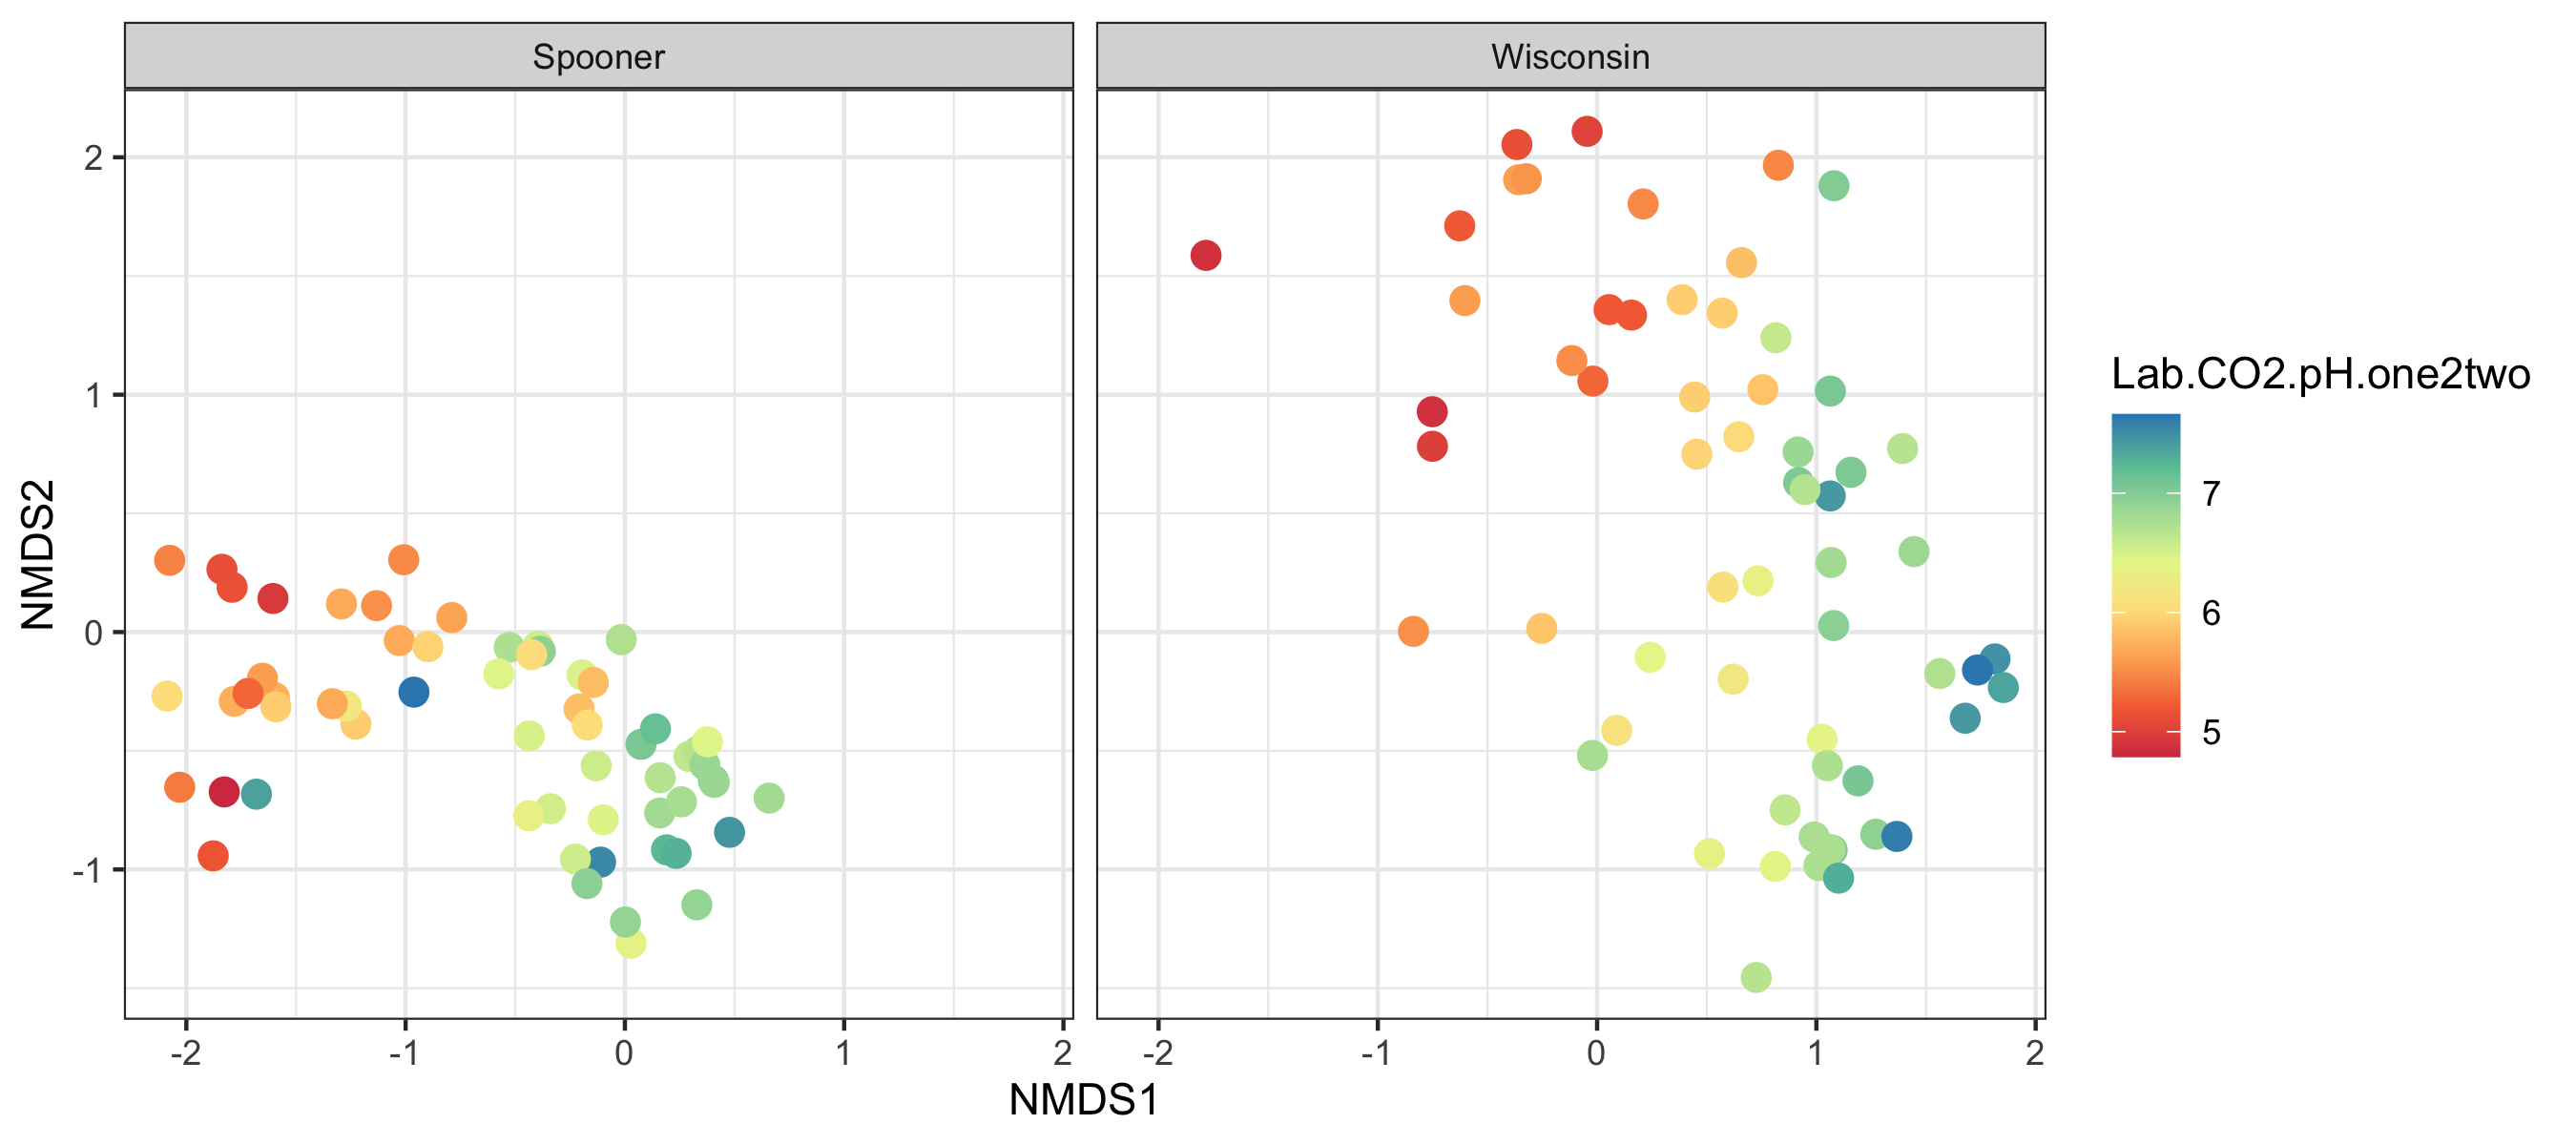
\includegraphics{output-rmd/nmds-bray-soilph-Lab.CO2.pH.one2two-1.png}

\begin{Shaded}
\begin{Highlighting}[]
\NormalTok{ps.ord.nmds =}\StringTok{ }\KeywordTok{ordinate}\NormalTok{(ps.norm, }\StringTok{"NMDS"}\NormalTok{, }\StringTok{"bray"}\NormalTok{,}\DataTypeTok{trymax=}\DecValTok{1000}\NormalTok{,}\DataTypeTok{k=}\DecValTok{3}\NormalTok{)}
\end{Highlighting}
\end{Shaded}

\begin{verbatim}
## Run 0 stress 0.1077299 
## Run 1 stress 0.1092029 
## Run 2 stress 0.1069171 
## ... New best solution
## ... Procrustes: rmse 0.00726917  max resid 0.07791938 
## Run 3 stress 0.1093431 
## Run 4 stress 0.1080699 
## Run 5 stress 0.1144399 
## Run 6 stress 0.1062303 
## ... New best solution
## ... Procrustes: rmse 0.006430935  max resid 0.06670596 
## Run 7 stress 0.1077258 
## Run 8 stress 0.1139906 
## Run 9 stress 0.109203 
## Run 10 stress 0.1115327 
## Run 11 stress 0.1111465 
## Run 12 stress 0.1124179 
## Run 13 stress 0.1128584 
## Run 14 stress 0.1091048 
## Run 15 stress 0.1106371 
## Run 16 stress 0.1071655 
## Run 17 stress 0.1092379 
## Run 18 stress 0.1093682 
## Run 19 stress 0.1143651 
## Run 20 stress 0.1093339 
## Run 21 stress 0.1093397 
## Run 22 stress 0.1108196 
## Run 23 stress 0.1092021 
## Run 24 stress 0.112283 
## Run 25 stress 0.1105506 
## Run 26 stress 0.1111652 
## Run 27 stress 0.1087668 
## Run 28 stress 0.1097707 
## Run 29 stress 0.111256 
## Run 30 stress 0.1109354 
## Run 31 stress 0.111803 
## Run 32 stress 0.1080736 
## Run 33 stress 0.1099536 
## Run 34 stress 0.10947 
## Run 35 stress 0.1109173 
## Run 36 stress 0.1094513 
## Run 37 stress 0.1092505 
## Run 38 stress 0.1091018 
## Run 39 stress 0.1106403 
## Run 40 stress 0.109263 
## Run 41 stress 0.1085864 
## Run 42 stress 0.1094456 
## Run 43 stress 0.1105605 
## Run 44 stress 0.1107981 
## Run 45 stress 0.1112406 
## Run 46 stress 0.1109157 
## Run 47 stress 0.1105099 
## Run 48 stress 0.1094408 
## Run 49 stress 0.1122964 
## Run 50 stress 0.1102929 
## Run 51 stress 0.1094315 
## Run 52 stress 0.1069118 
## Run 53 stress 0.1062347 
## ... Procrustes: rmse 0.001146508  max resid 0.00875042 
## ... Similar to previous best
## *** Solution reached
\end{verbatim}

\begin{Shaded}
\begin{Highlighting}[]
\NormalTok{p =}\StringTok{ }\KeywordTok{plot_ordination}\NormalTok{(ps.norm, ps.ord.nmds, }\DataTypeTok{type=}\StringTok{"samples"}\NormalTok{)}
\NormalTok{palette =}\StringTok{ }\KeywordTok{brewer.pal}\NormalTok{(}\DecValTok{8}\NormalTok{, }\StringTok{"Spectral"}\NormalTok{)}
\NormalTok{p =}\StringTok{ }\NormalTok{p }\OperatorTok{+}\StringTok{ }\KeywordTok{aes}\NormalTok{(}\DataTypeTok{colour=}\NormalTok{Lab.CO2.pH.one2three) }\OperatorTok{+}\StringTok{ }\KeywordTok{geom_point}\NormalTok{(}\DataTypeTok{size=}\DecValTok{3}\NormalTok{) }\OperatorTok{+}\StringTok{ }
\StringTok{  }\KeywordTok{scale_colour_gradientn}\NormalTok{(}\DataTypeTok{colors=}\NormalTok{palette) }\OperatorTok{+}\StringTok{ }\KeywordTok{facet_wrap}\NormalTok{(}\OperatorTok{~}\NormalTok{Study) }\OperatorTok{+}\StringTok{ }
\StringTok{  }\KeywordTok{theme_bw}\NormalTok{()}
\NormalTok{p}
\end{Highlighting}
\end{Shaded}

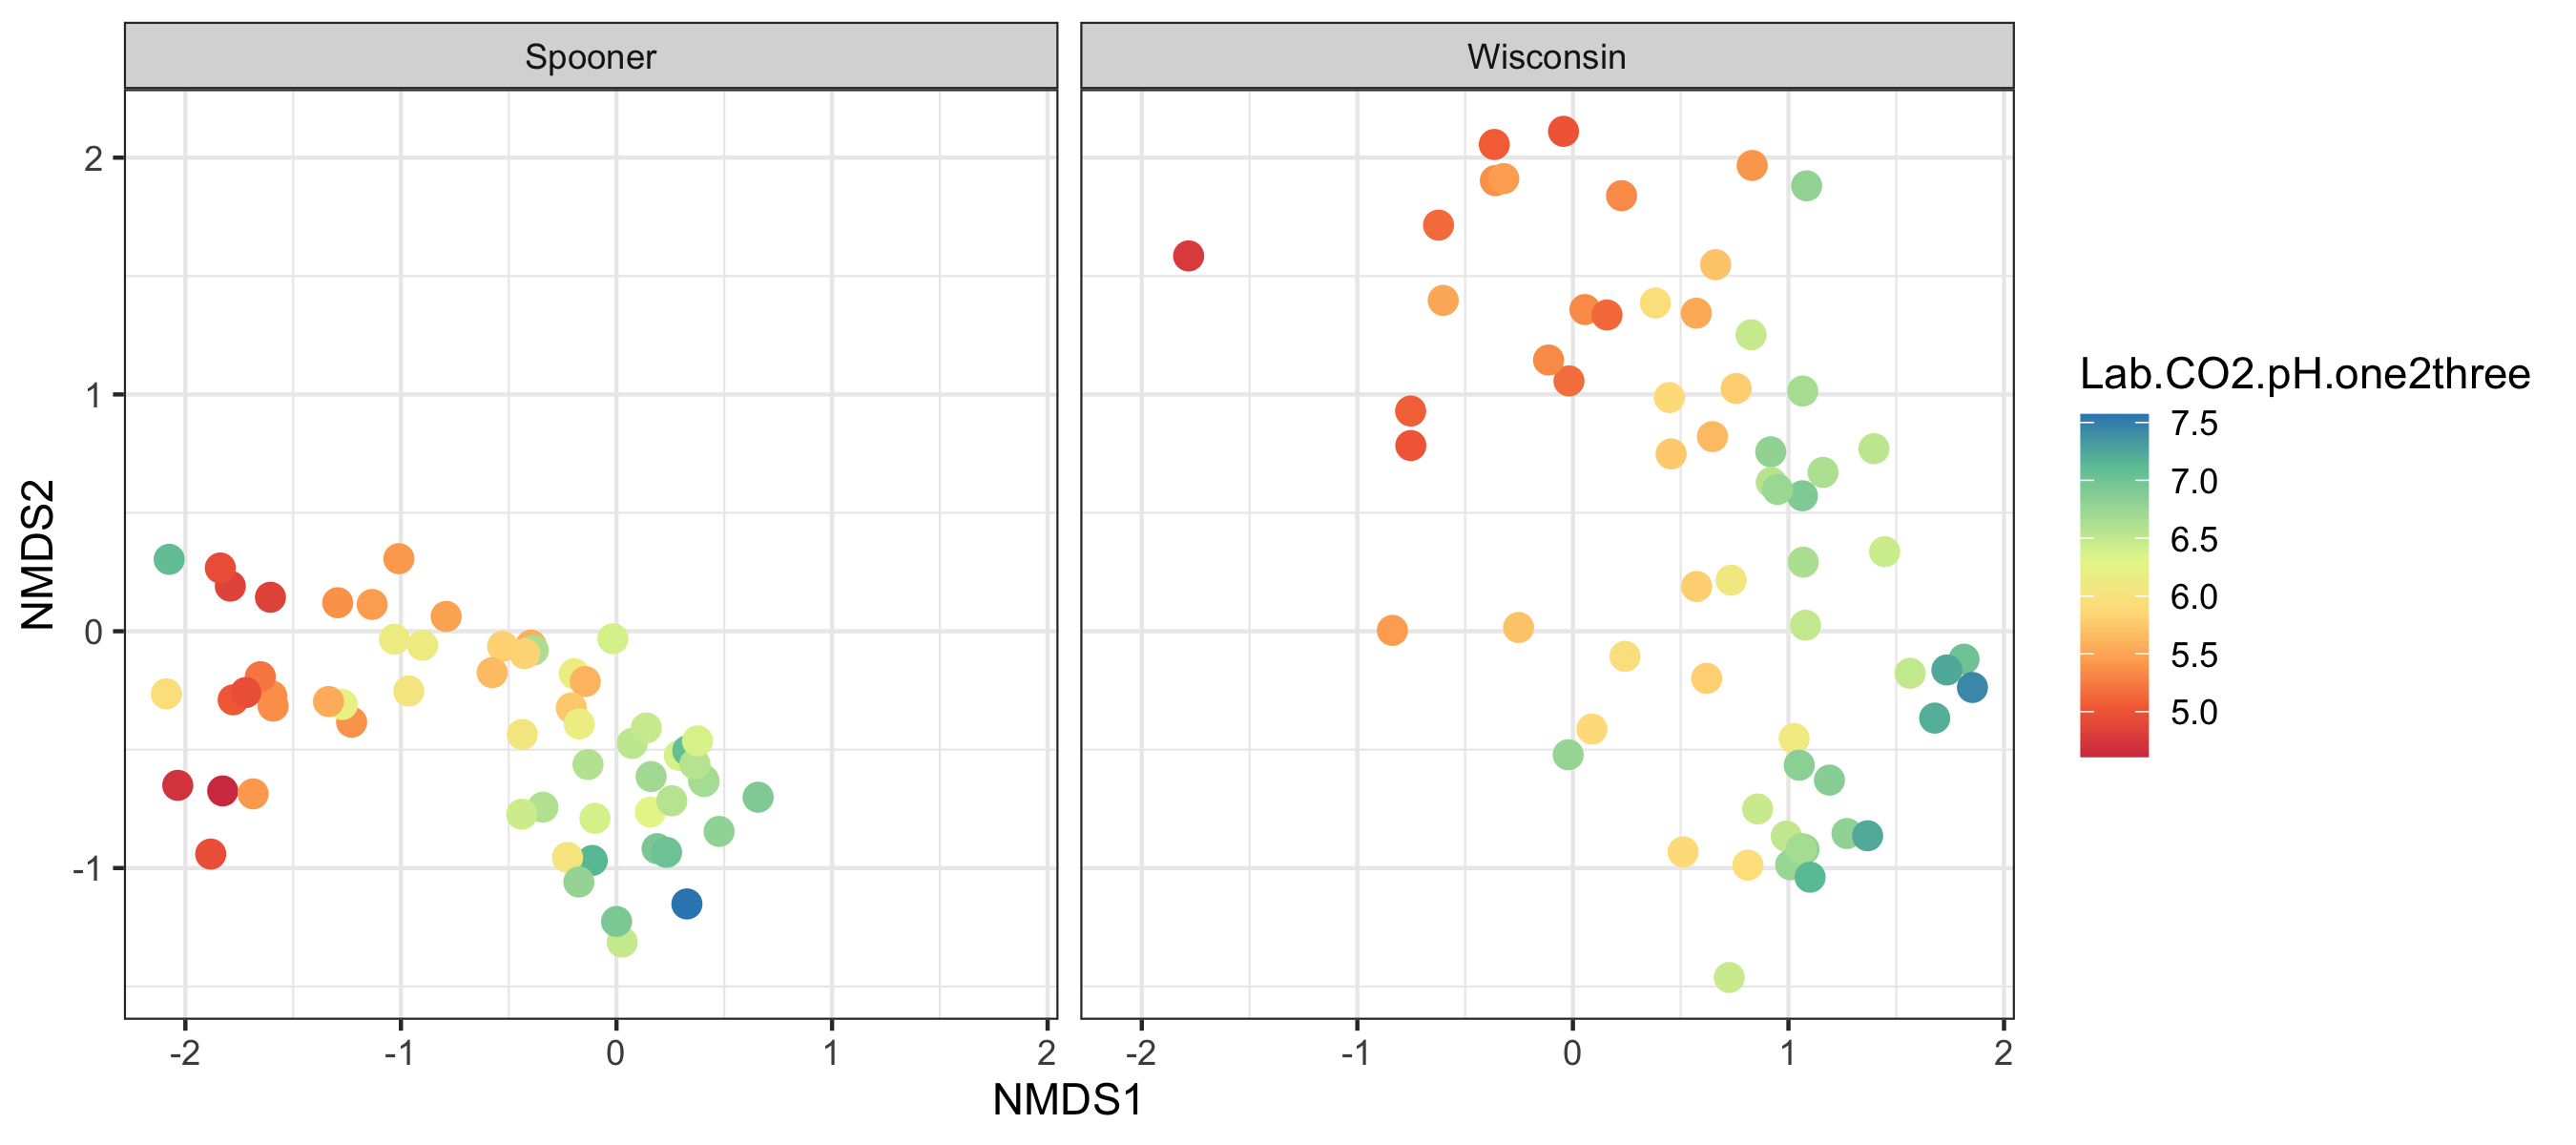
\includegraphics{output-rmd/nmds-bray-soilph-Lab.CO2.pH.one2thre-1.png}

\begin{Shaded}
\begin{Highlighting}[]
\NormalTok{ps.ord.nmds =}\StringTok{ }\KeywordTok{ordinate}\NormalTok{(ps.norm, }\StringTok{"NMDS"}\NormalTok{, }\StringTok{"bray"}\NormalTok{,}\DataTypeTok{trymax=}\DecValTok{1000}\NormalTok{,}\DataTypeTok{k=}\DecValTok{3}\NormalTok{)}
\end{Highlighting}
\end{Shaded}

\begin{verbatim}
## Run 0 stress 0.1077299 
## Run 1 stress 0.111801 
## Run 2 stress 0.1073872 
## ... New best solution
## ... Procrustes: rmse 0.009287425  max resid 0.07734785 
## Run 3 stress 0.1105522 
## Run 4 stress 0.1104812 
## Run 5 stress 0.1137769 
## Run 6 stress 0.1095989 
## Run 7 stress 0.1112492 
## Run 8 stress 0.1078906 
## Run 9 stress 0.1088104 
## Run 10 stress 0.1106 
## Run 11 stress 0.1102486 
## Run 12 stress 0.1085066 
## Run 13 stress 0.1097292 
## Run 14 stress 0.1085885 
## Run 15 stress 0.1108186 
## Run 16 stress 0.1112486 
## Run 17 stress 0.1109846 
## Run 18 stress 0.1119729 
## Run 19 stress 0.1109225 
## Run 20 stress 0.108043 
## Run 21 stress 0.1062276 
## ... New best solution
## ... Procrustes: rmse 0.008551883  max resid 0.06883626 
## Run 22 stress 0.1096065 
## Run 23 stress 0.1092481 
## Run 24 stress 0.1113343 
## Run 25 stress 0.1106847 
## Run 26 stress 0.1109521 
## Run 27 stress 0.108317 
## Run 28 stress 0.1071662 
## Run 29 stress 0.1105536 
## Run 30 stress 0.1062267 
## ... New best solution
## ... Procrustes: rmse 0.0001598635  max resid 0.001335009 
## ... Similar to previous best
## *** Solution reached
\end{verbatim}

\begin{Shaded}
\begin{Highlighting}[]
\NormalTok{p =}\StringTok{ }\KeywordTok{plot_ordination}\NormalTok{(ps.norm, ps.ord.nmds, }\DataTypeTok{type=}\StringTok{"samples"}\NormalTok{)}
\NormalTok{palette =}\StringTok{ }\KeywordTok{brewer.pal}\NormalTok{(}\DecValTok{8}\NormalTok{, }\StringTok{"Spectral"}\NormalTok{)}
\NormalTok{p =}\StringTok{ }\NormalTok{p }\OperatorTok{+}\StringTok{ }\KeywordTok{aes}\NormalTok{(}\DataTypeTok{colour=}\NormalTok{Lab.CO2.pH.one2four) }\OperatorTok{+}\StringTok{ }\KeywordTok{geom_point}\NormalTok{(}\DataTypeTok{size=}\DecValTok{3}\NormalTok{) }\OperatorTok{+}\StringTok{ }
\StringTok{  }\KeywordTok{scale_colour_gradientn}\NormalTok{(}\DataTypeTok{colors=}\NormalTok{palette) }\OperatorTok{+}\StringTok{ }\KeywordTok{facet_wrap}\NormalTok{(}\OperatorTok{~}\NormalTok{Study) }\OperatorTok{+}\StringTok{ }
\StringTok{  }\KeywordTok{theme_bw}\NormalTok{()}
\NormalTok{p}
\end{Highlighting}
\end{Shaded}

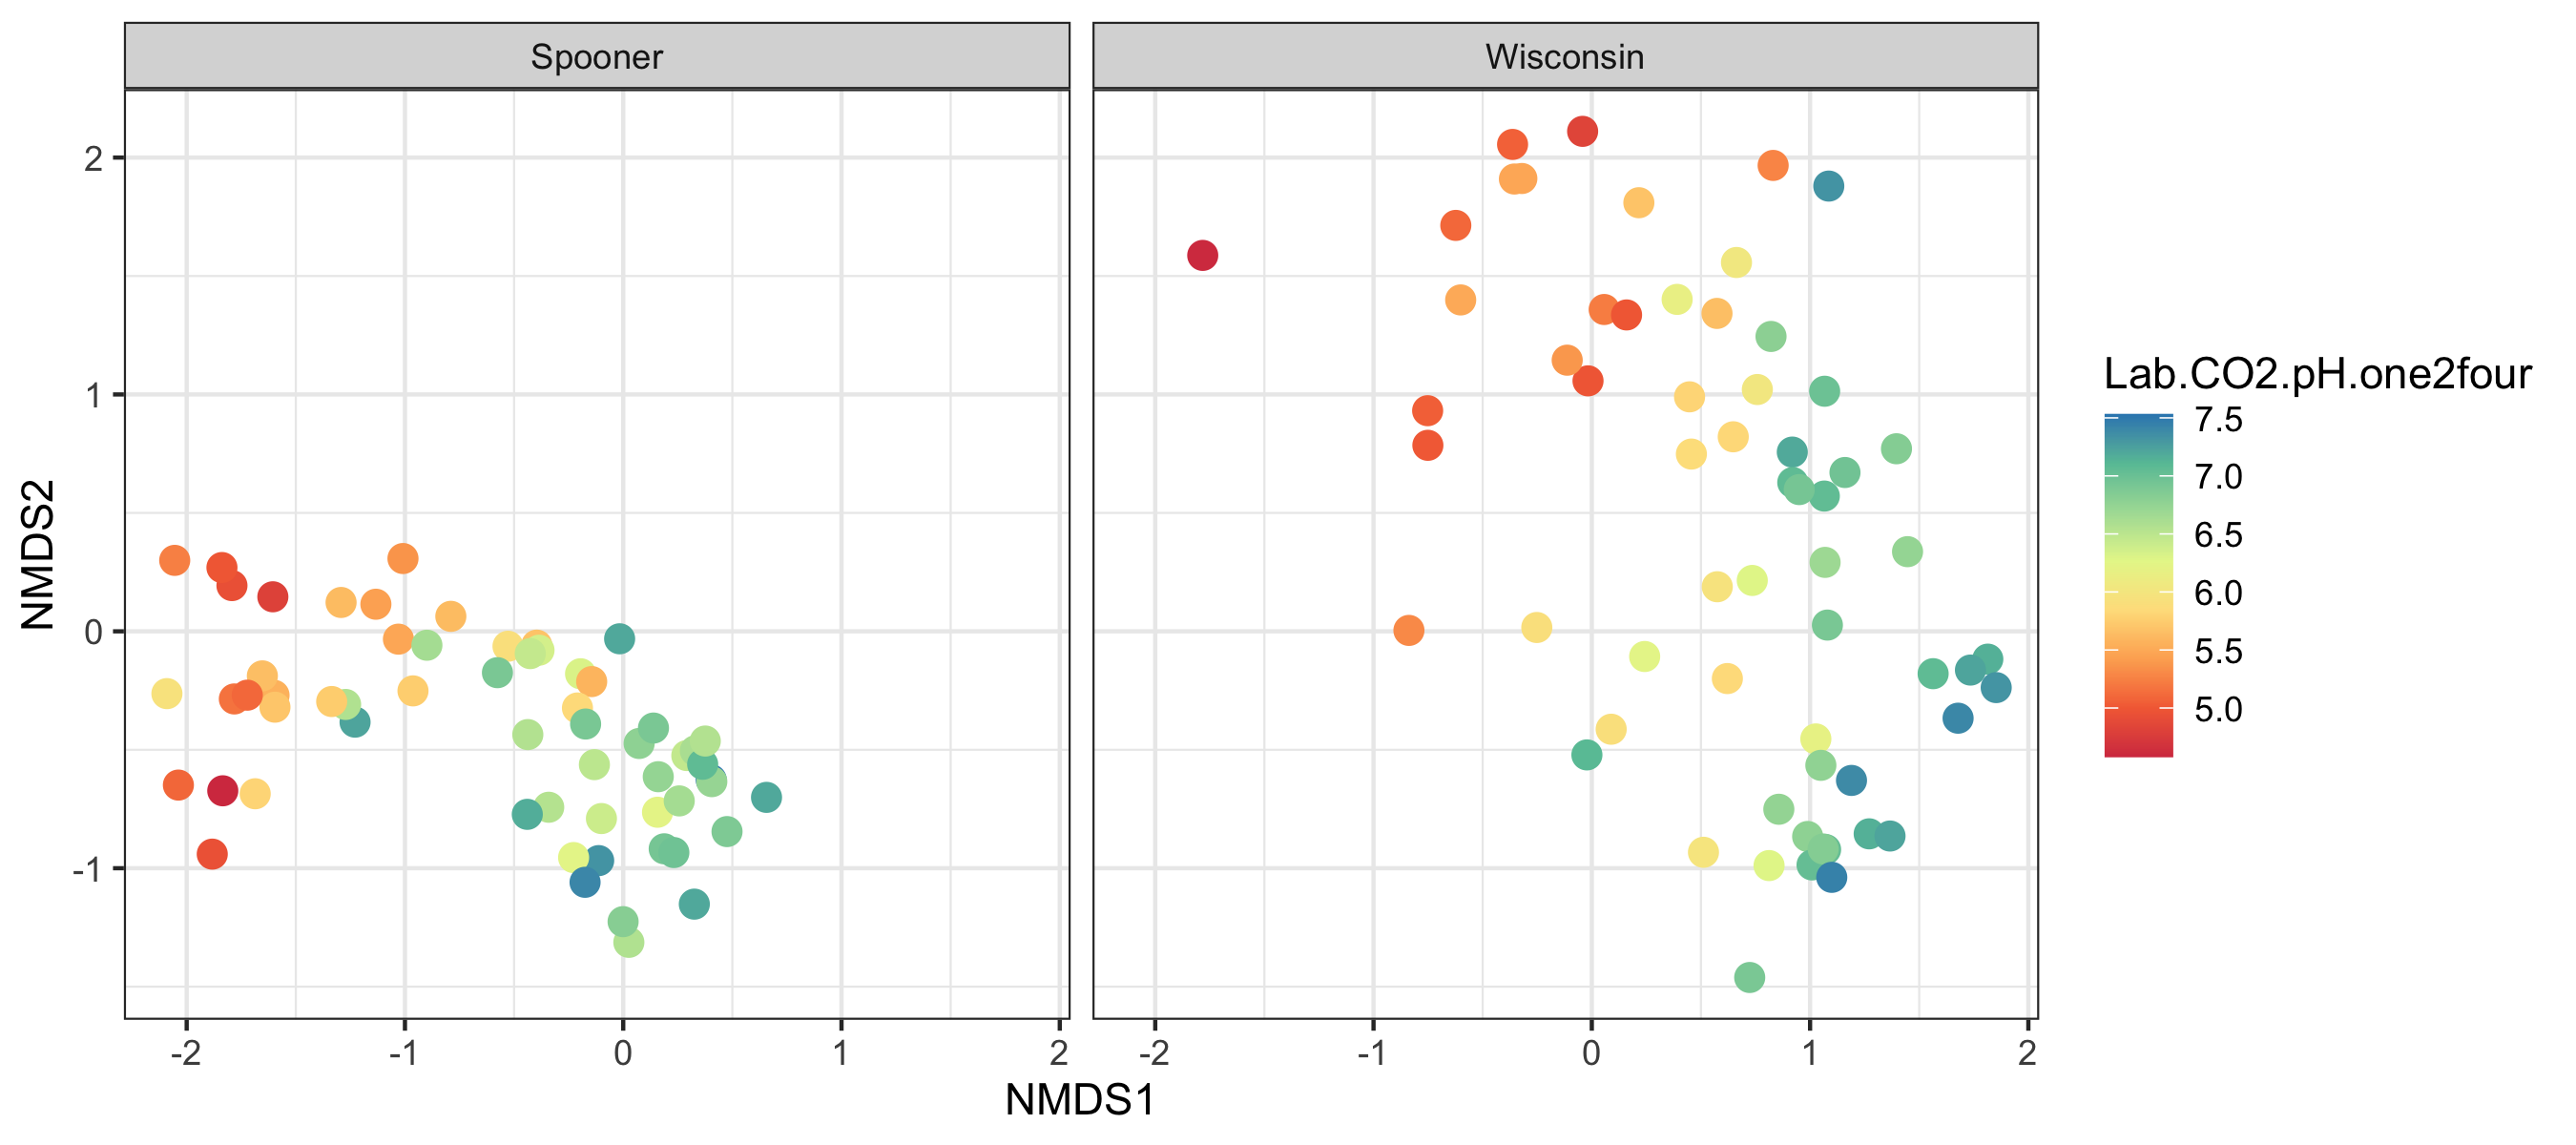
\includegraphics{output-rmd/nmds-bray-soilph-Lab.CO2.pH.one2four-1.png}

\begin{Shaded}
\begin{Highlighting}[]
\NormalTok{p <-}\StringTok{ }\KeywordTok{plot_richness}\NormalTok{(ps, }\DataTypeTok{x=}\StringTok{"Lab.CO2.pH.one2one"}\NormalTok{, }\DataTypeTok{measures=}\KeywordTok{c}\NormalTok{(}\StringTok{"Observed"}\NormalTok{,}\StringTok{"Simpson"}\NormalTok{,}\StringTok{"Shannon"}\NormalTok{), }\DataTypeTok{scales =} \StringTok{"free_y"}\NormalTok{, }\DataTypeTok{shape=}\StringTok{"Study"}\NormalTok{)}
\NormalTok{p }\OperatorTok{+}\StringTok{ }\KeywordTok{geom_point}\NormalTok{(}\DataTypeTok{size=}\DecValTok{4}\NormalTok{, }\DataTypeTok{alpha=}\FloatTok{0.2}\NormalTok{) }\OperatorTok{+}\StringTok{ }\KeywordTok{theme_bw}\NormalTok{()}
\end{Highlighting}
\end{Shaded}

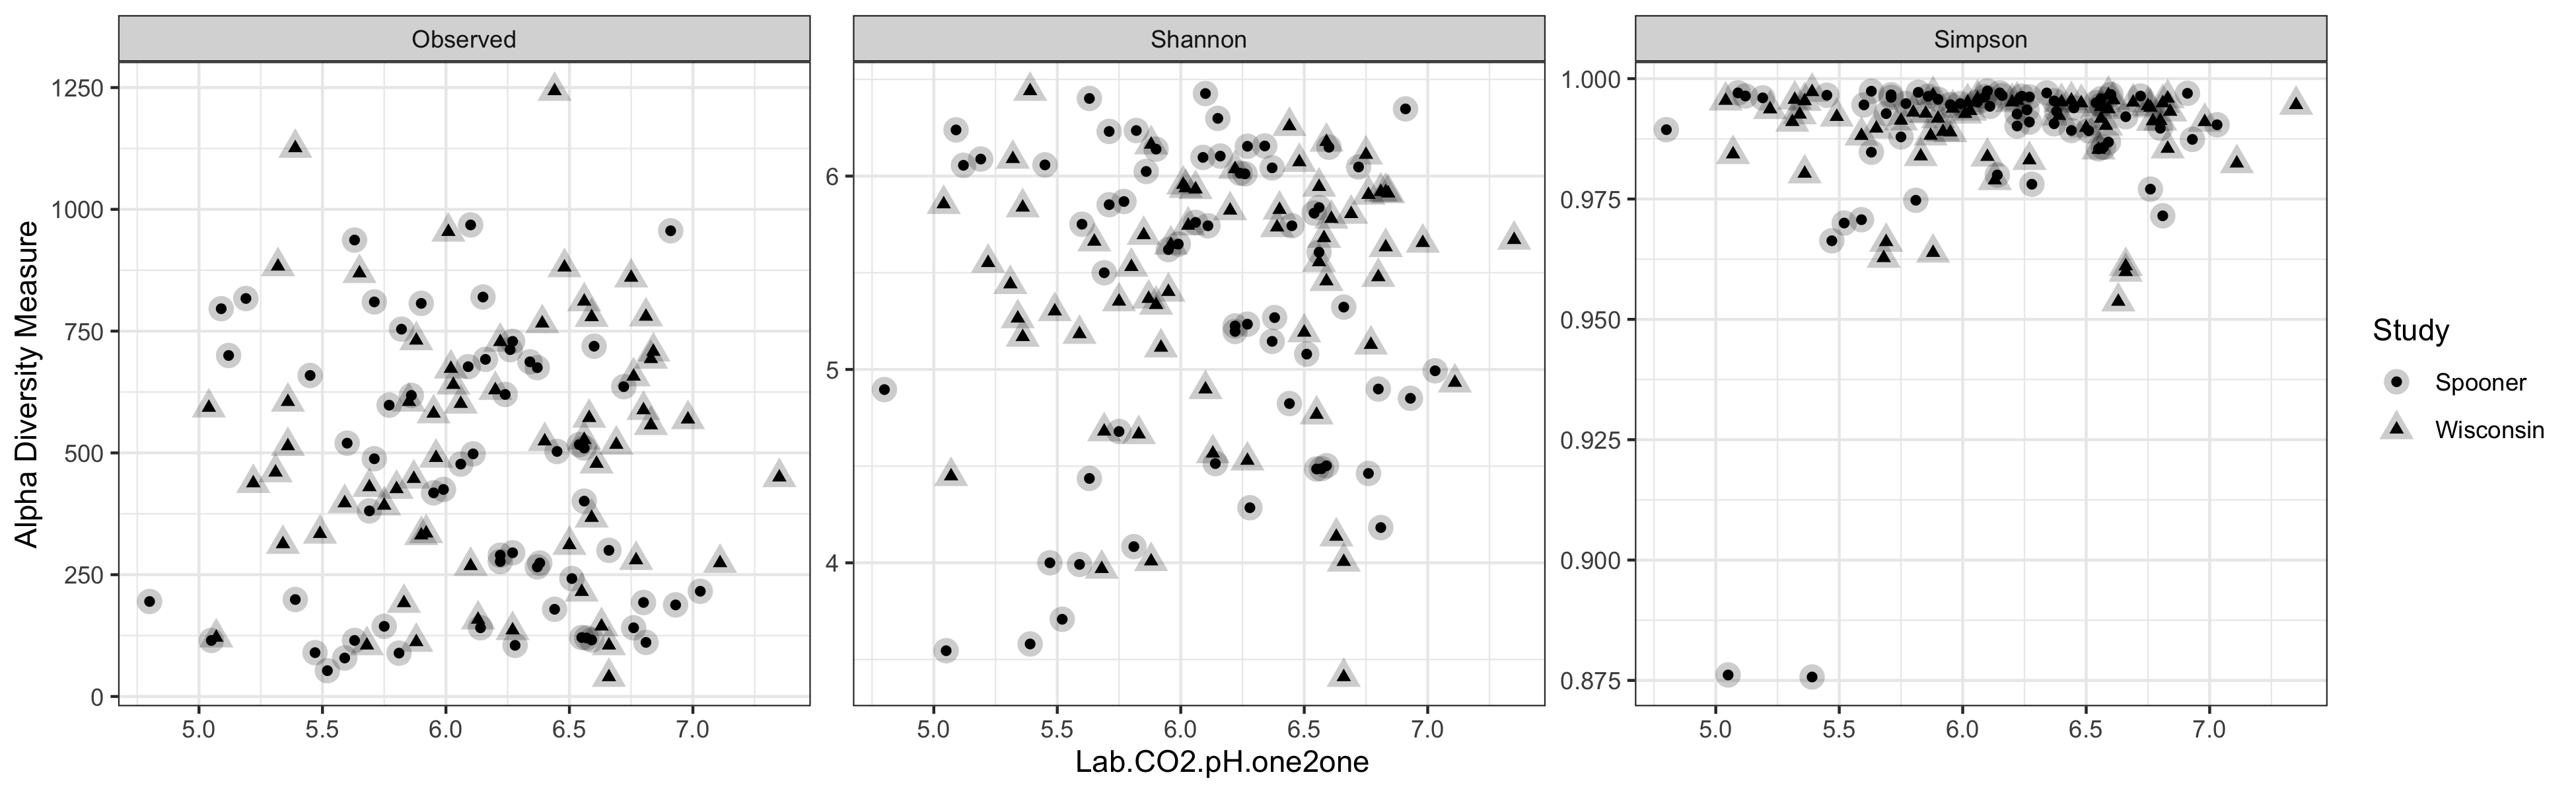
\includegraphics{output-rmd/richness-ph-Lab.CO2.pH.one2one-1.png}

\begin{Shaded}
\begin{Highlighting}[]
\NormalTok{p <-}\StringTok{ }\KeywordTok{plot_richness}\NormalTok{(ps, }\DataTypeTok{x=}\StringTok{"Lab.CO2.pH.one2two"}\NormalTok{, }\DataTypeTok{measures=}\KeywordTok{c}\NormalTok{(}\StringTok{"Observed"}\NormalTok{,}\StringTok{"Simpson"}\NormalTok{,}\StringTok{"Shannon"}\NormalTok{), }\DataTypeTok{scales =} \StringTok{"free_y"}\NormalTok{, }\DataTypeTok{shape=}\StringTok{"Study"}\NormalTok{)}
\NormalTok{p }\OperatorTok{+}\StringTok{ }\KeywordTok{geom_point}\NormalTok{(}\DataTypeTok{size=}\DecValTok{4}\NormalTok{, }\DataTypeTok{alpha=}\FloatTok{0.2}\NormalTok{) }\OperatorTok{+}\StringTok{ }\KeywordTok{theme_bw}\NormalTok{()}
\end{Highlighting}
\end{Shaded}

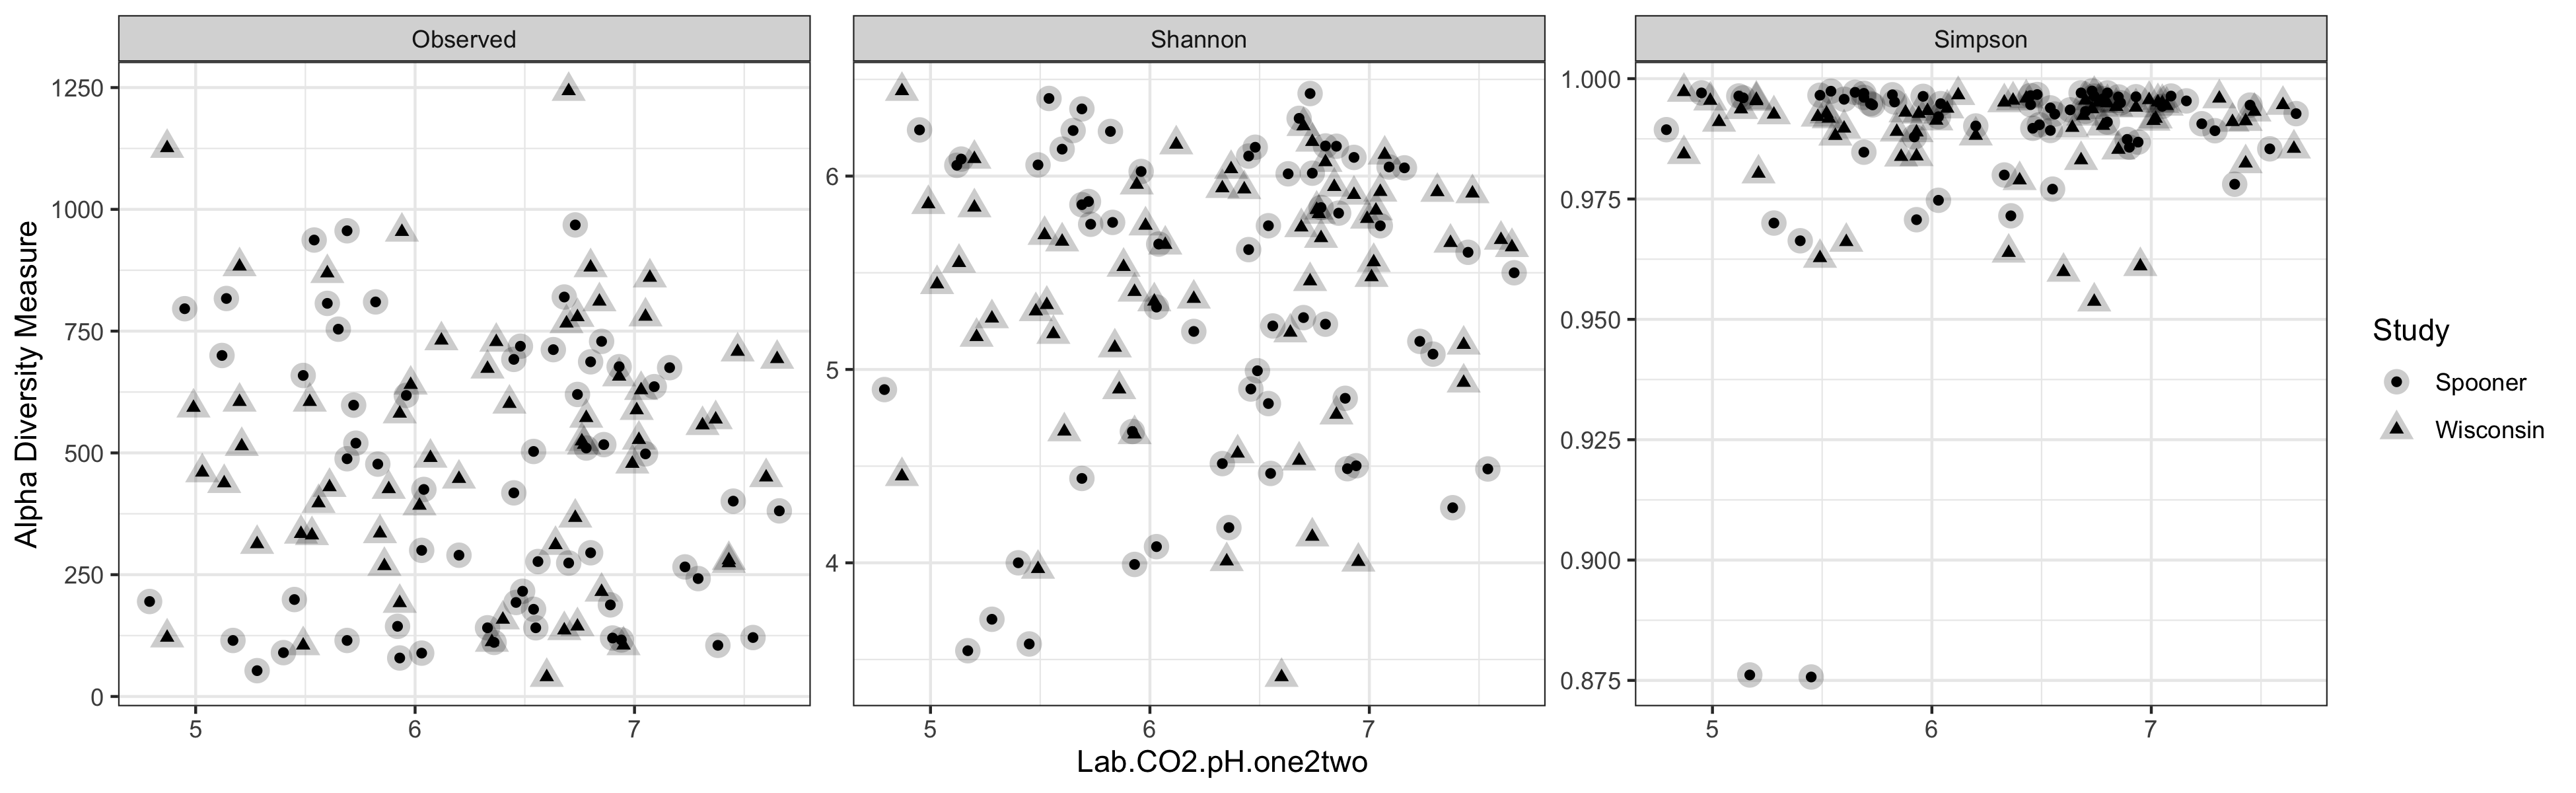
\includegraphics{output-rmd/richness-ph-Lab.CO2.pH.one2two-1.png}

\begin{Shaded}
\begin{Highlighting}[]
\NormalTok{p <-}\StringTok{ }\KeywordTok{plot_richness}\NormalTok{(ps, }\DataTypeTok{x=}\StringTok{"Lab.CO2.pH.one2three"}\NormalTok{, }\DataTypeTok{measures=}\KeywordTok{c}\NormalTok{(}\StringTok{"Observed"}\NormalTok{,}\StringTok{"Simpson"}\NormalTok{,}\StringTok{"Shannon"}\NormalTok{), }\DataTypeTok{scales =} \StringTok{"free_y"}\NormalTok{, }\DataTypeTok{shape=}\StringTok{"Study"}\NormalTok{)}
\NormalTok{p }\OperatorTok{+}\StringTok{ }\KeywordTok{geom_point}\NormalTok{(}\DataTypeTok{size=}\DecValTok{4}\NormalTok{, }\DataTypeTok{alpha=}\FloatTok{0.2}\NormalTok{) }\OperatorTok{+}\StringTok{ }\KeywordTok{theme_bw}\NormalTok{()}
\end{Highlighting}
\end{Shaded}

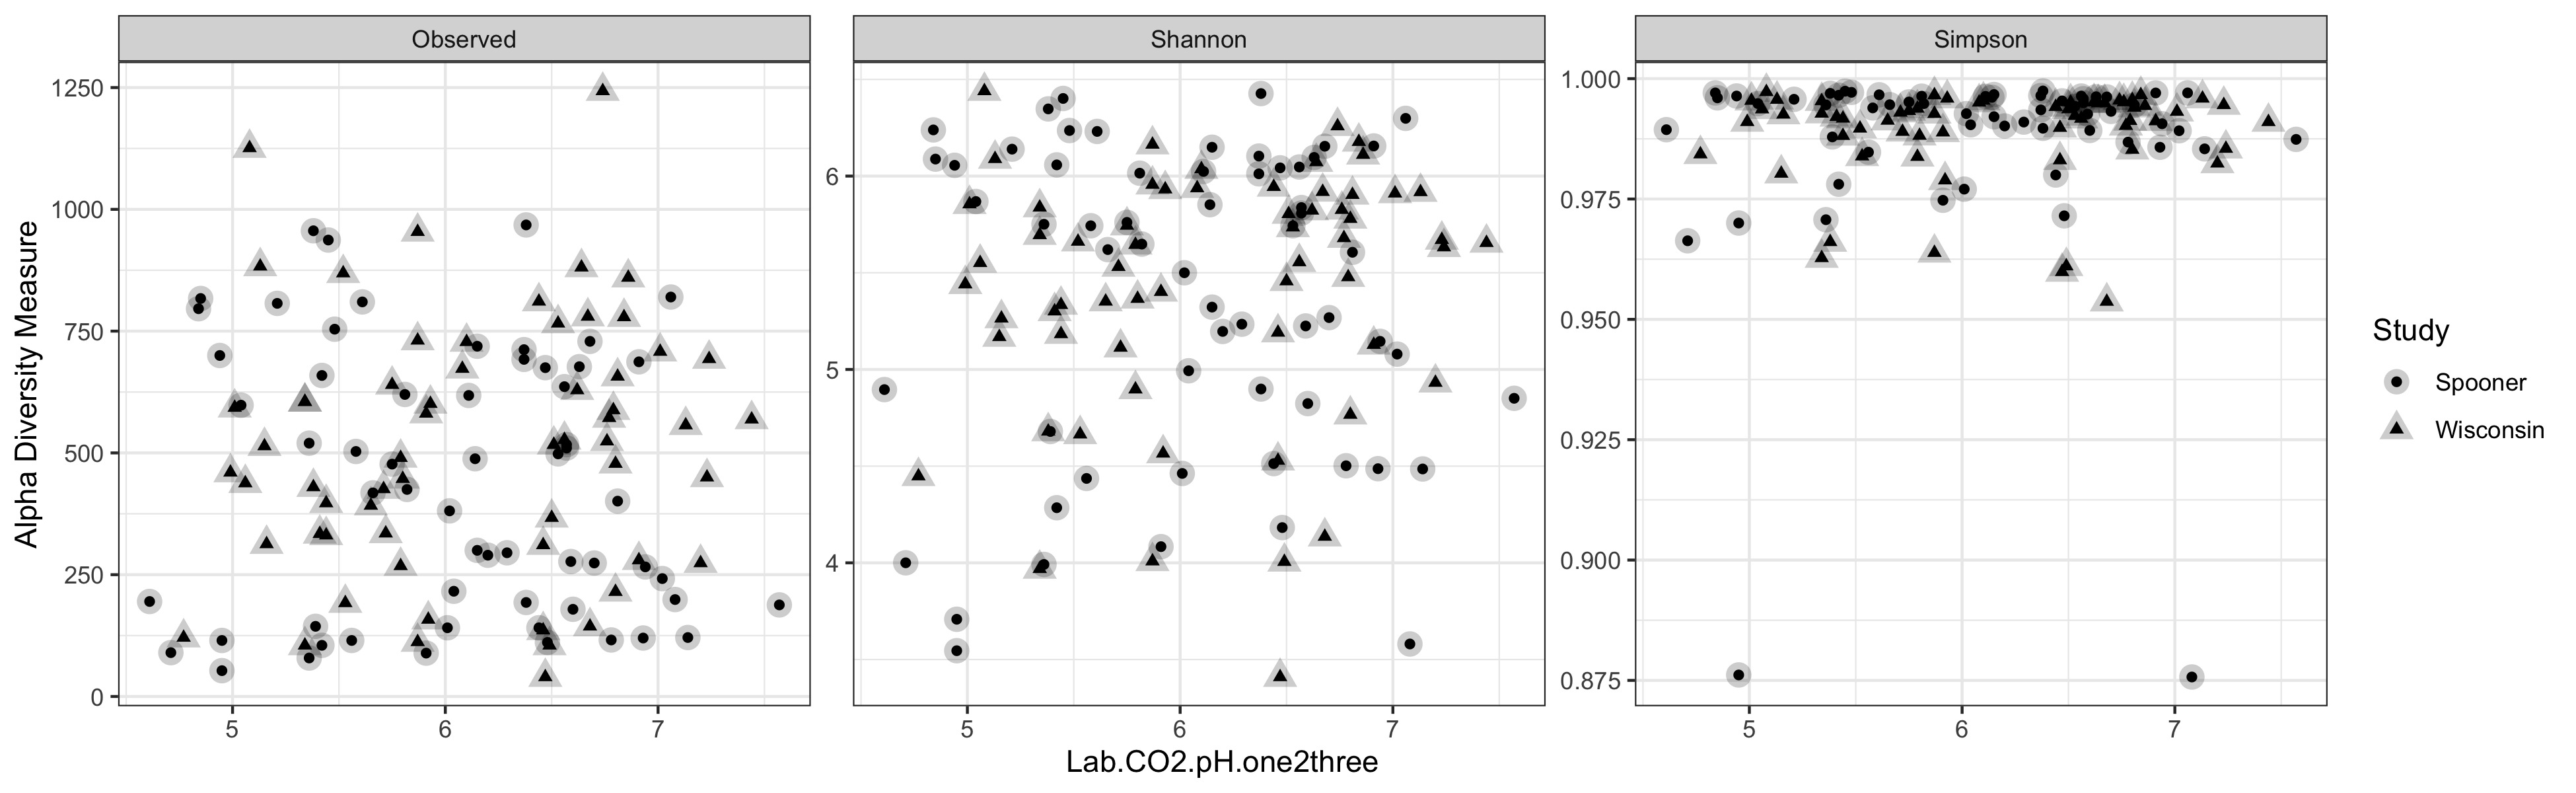
\includegraphics{output-rmd/richness-ph-Lab.CO2.pH.one2three-1.png}

\begin{Shaded}
\begin{Highlighting}[]
\NormalTok{p <-}\StringTok{ }\KeywordTok{plot_richness}\NormalTok{(ps, }\DataTypeTok{x=}\StringTok{"Lab.CO2.pH.one2four"}\NormalTok{, }\DataTypeTok{measures=}\KeywordTok{c}\NormalTok{(}\StringTok{"Observed"}\NormalTok{,}\StringTok{"Simpson"}\NormalTok{,}\StringTok{"Shannon"}\NormalTok{), }\DataTypeTok{scales =} \StringTok{"free_y"}\NormalTok{, }\DataTypeTok{shape=}\StringTok{"Study"}\NormalTok{)}
\NormalTok{p }\OperatorTok{+}\StringTok{ }\KeywordTok{geom_point}\NormalTok{(}\DataTypeTok{size=}\DecValTok{4}\NormalTok{, }\DataTypeTok{alpha=}\FloatTok{0.2}\NormalTok{) }\OperatorTok{+}\StringTok{ }\KeywordTok{theme_bw}\NormalTok{()}
\end{Highlighting}
\end{Shaded}

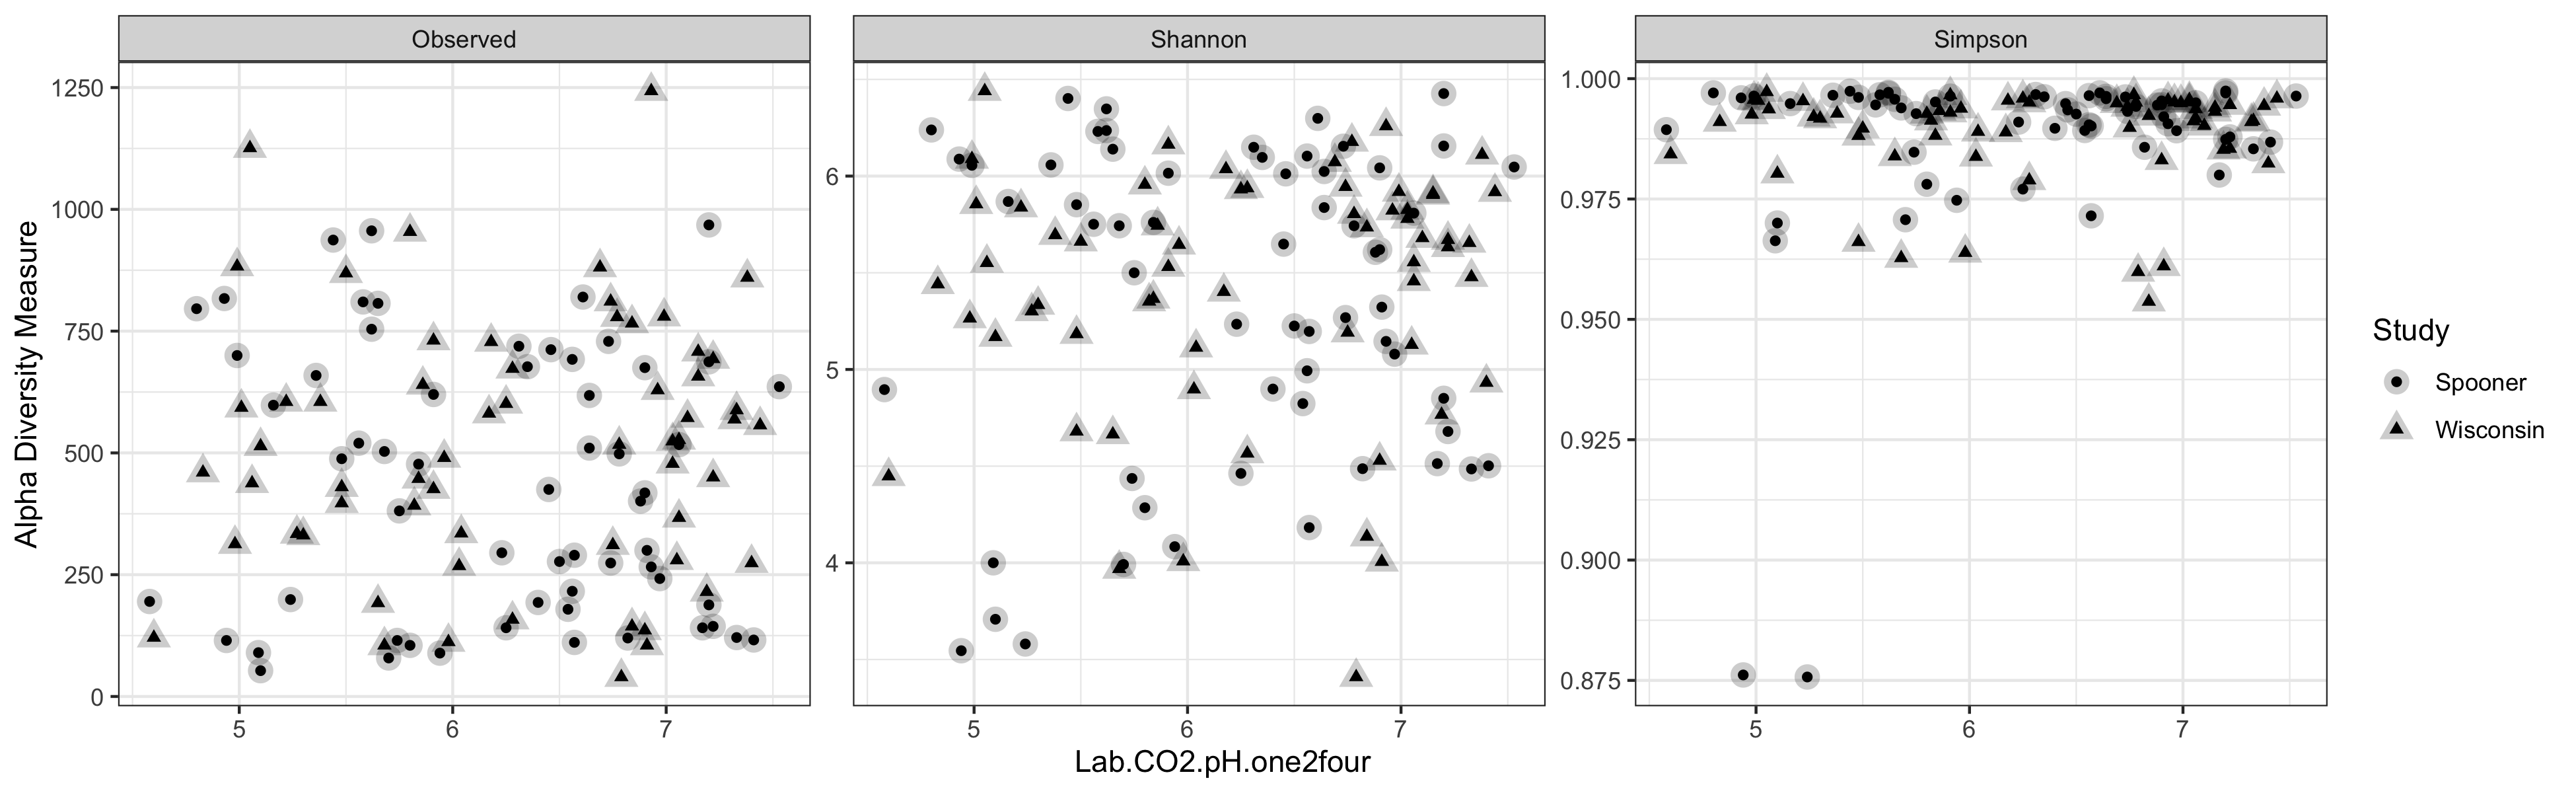
\includegraphics{output-rmd/richness-ph-Lab.CO2.pH.one2four-1.png}

\begin{Shaded}
\begin{Highlighting}[]
\NormalTok{p <-}\StringTok{ }\KeywordTok{plot_richness}\NormalTok{(ps, }\DataTypeTok{x=}\StringTok{"Lab.CO2.Hplus.one2one"}\NormalTok{, }\DataTypeTok{measures=}\KeywordTok{c}\NormalTok{(}\StringTok{"Observed"}\NormalTok{,}\StringTok{"Simpson"}\NormalTok{,}\StringTok{"Shannon"}\NormalTok{), }\DataTypeTok{scales =} \StringTok{"free_y"}\NormalTok{, }\DataTypeTok{shape=}\StringTok{"Study"}\NormalTok{)}
\NormalTok{p }\OperatorTok{+}\StringTok{ }\KeywordTok{geom_point}\NormalTok{(}\DataTypeTok{size=}\DecValTok{4}\NormalTok{, }\DataTypeTok{alpha=}\FloatTok{0.2}\NormalTok{) }\OperatorTok{+}\StringTok{ }\KeywordTok{theme_bw}\NormalTok{()}
\end{Highlighting}
\end{Shaded}

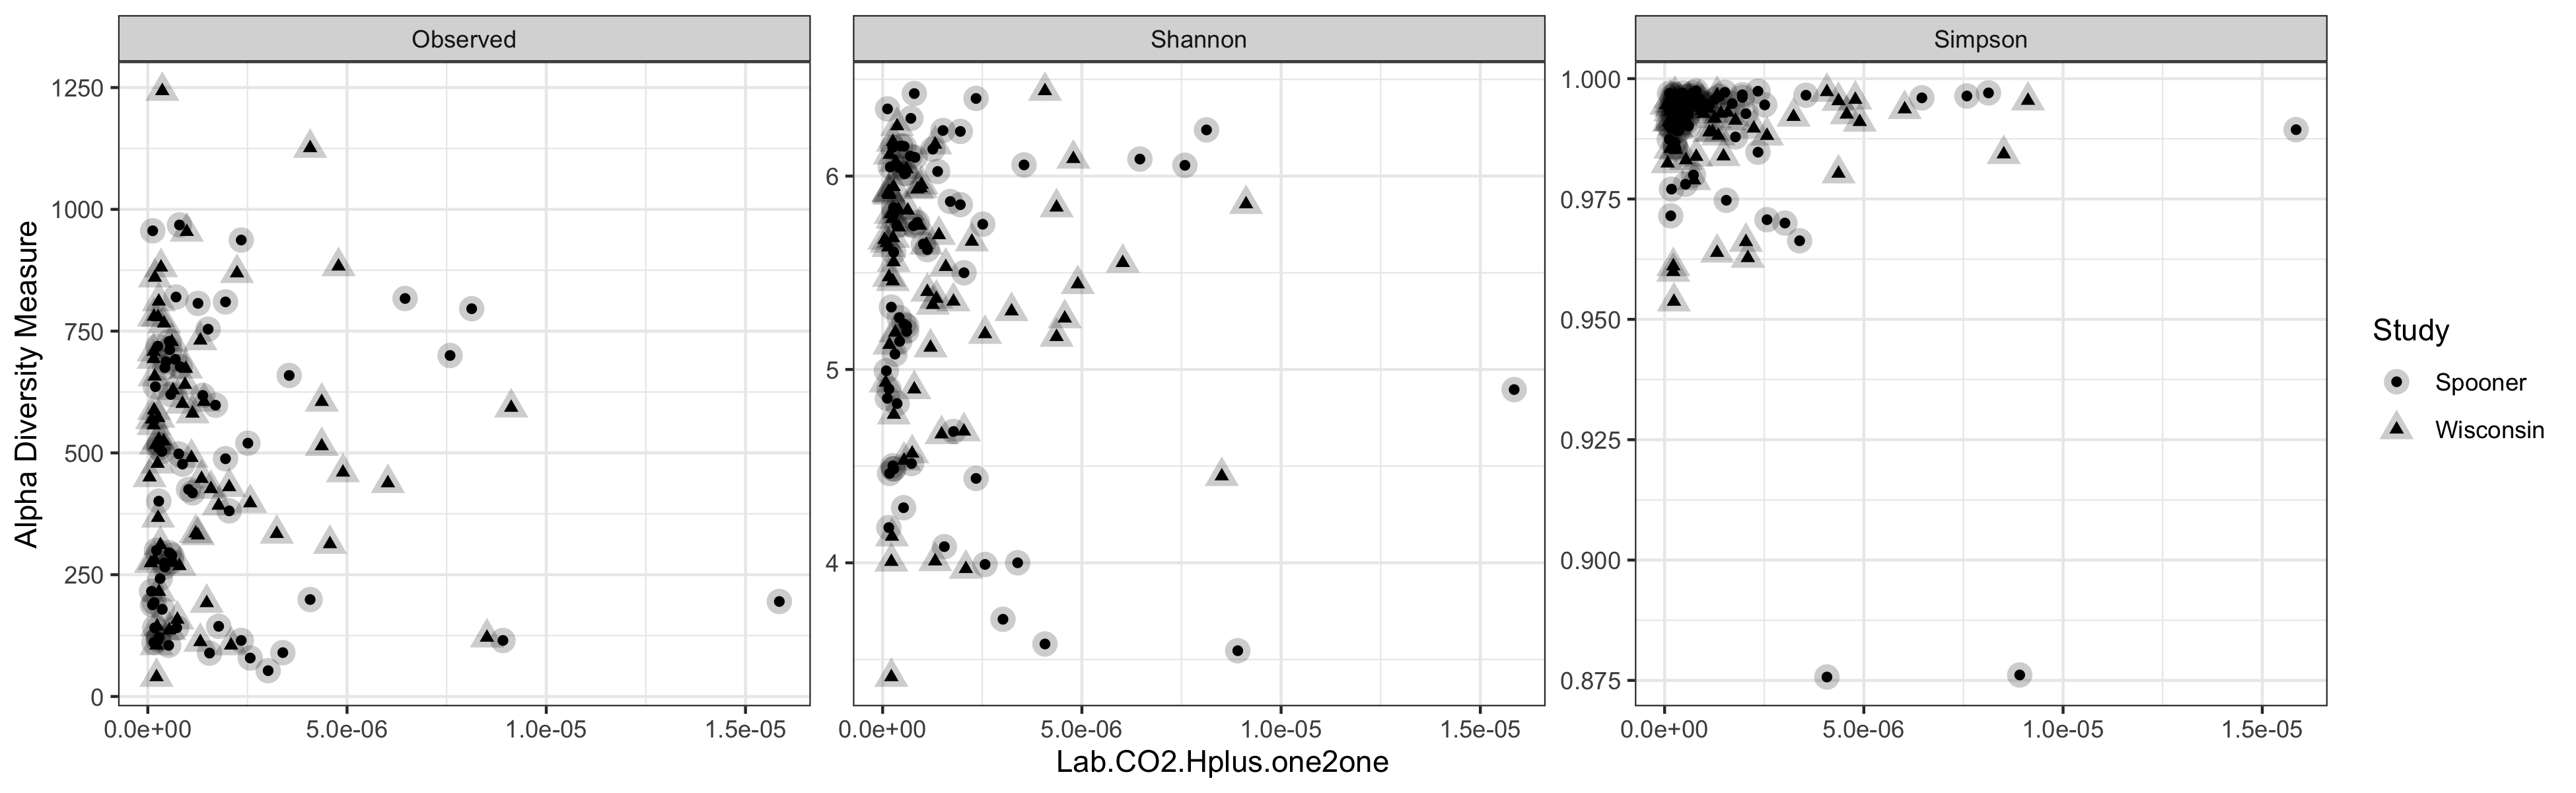
\includegraphics{output-rmd/richness-ph-Lab.CO2.Hplus.one2one-1.png}

\begin{Shaded}
\begin{Highlighting}[]
\NormalTok{p <-}\StringTok{ }\KeywordTok{plot_richness}\NormalTok{(ps, }\DataTypeTok{x=}\StringTok{"Lab.CO2.Hplus.one2two"}\NormalTok{, }\DataTypeTok{measures=}\KeywordTok{c}\NormalTok{(}\StringTok{"Observed"}\NormalTok{,}\StringTok{"Simpson"}\NormalTok{,}\StringTok{"Shannon"}\NormalTok{), }\DataTypeTok{scales =} \StringTok{"free_y"}\NormalTok{, }\DataTypeTok{shape=}\StringTok{"Study"}\NormalTok{)}
\NormalTok{p }\OperatorTok{+}\StringTok{ }\KeywordTok{geom_point}\NormalTok{(}\DataTypeTok{size=}\DecValTok{4}\NormalTok{, }\DataTypeTok{alpha=}\FloatTok{0.2}\NormalTok{) }\OperatorTok{+}\StringTok{ }\KeywordTok{theme_bw}\NormalTok{()}
\end{Highlighting}
\end{Shaded}

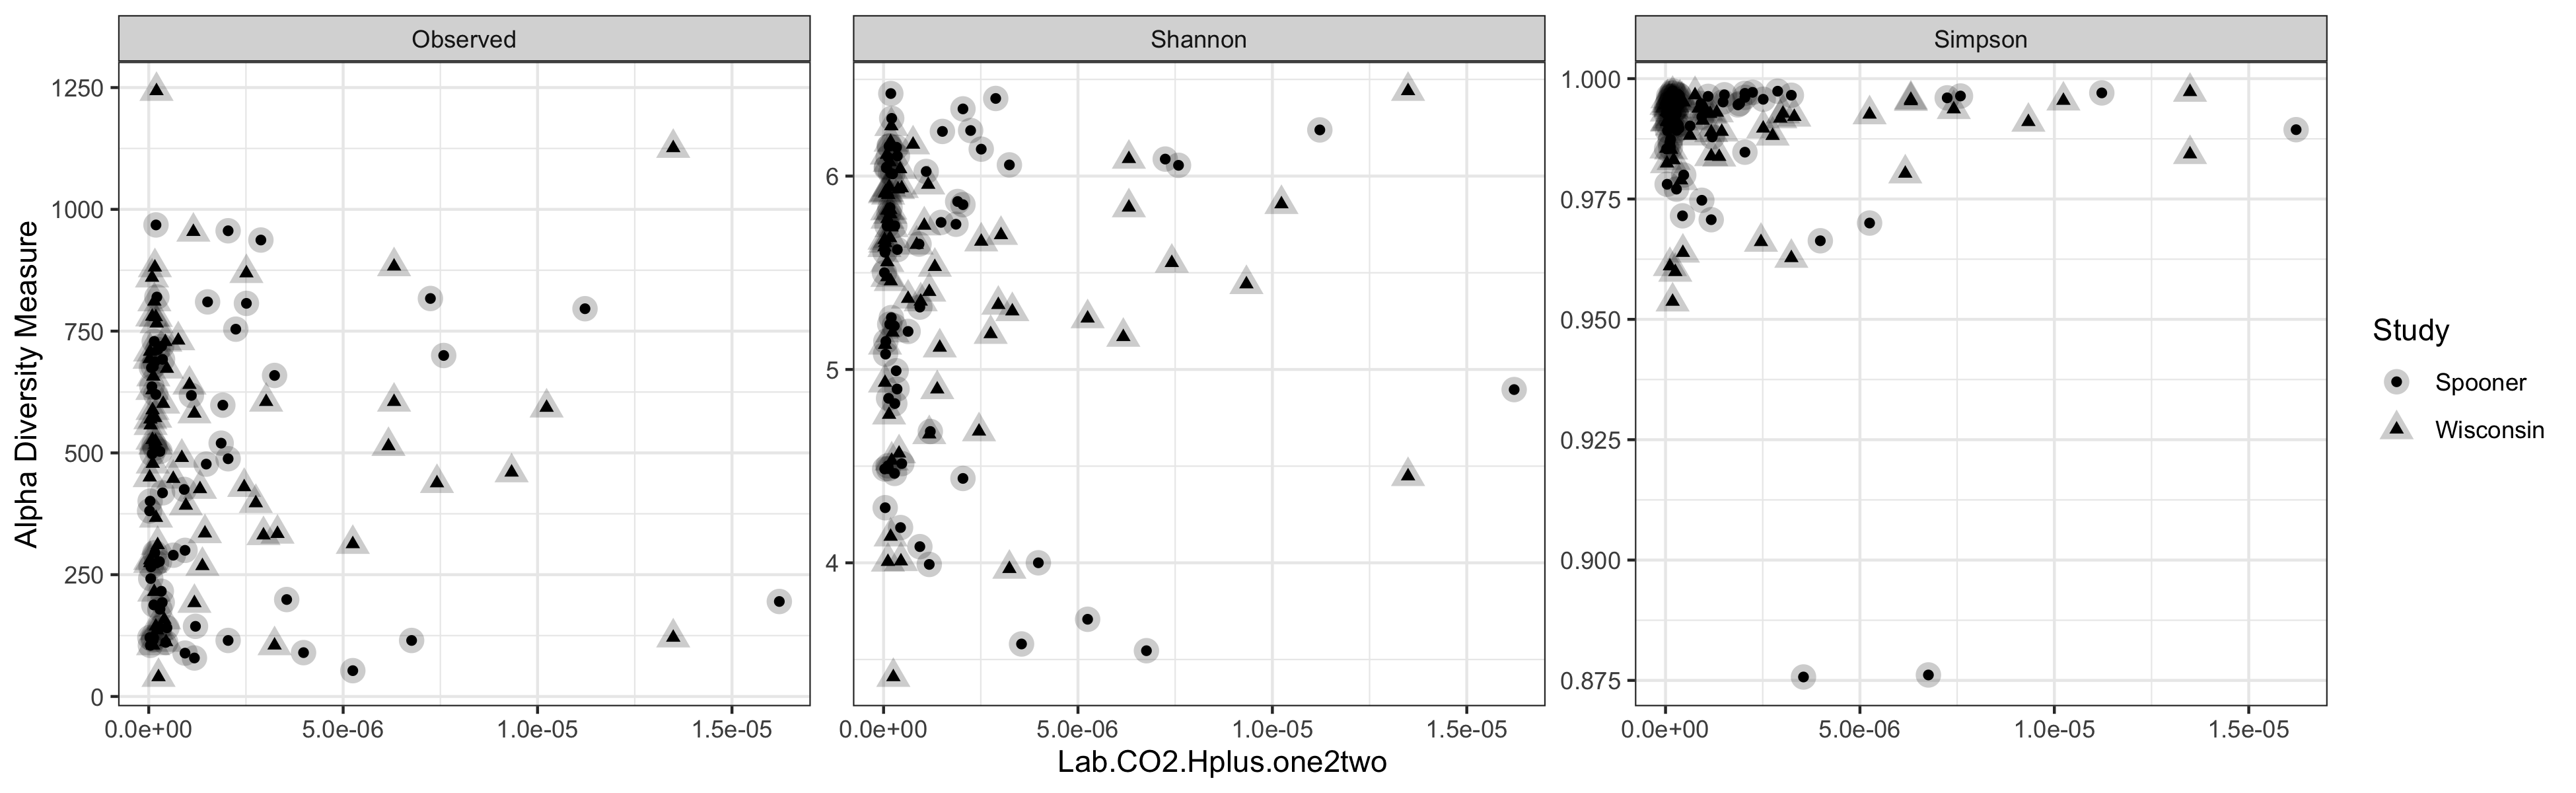
\includegraphics{output-rmd/richness-ph-Lab.CO2.Hplus.one2two-1.png}

\begin{Shaded}
\begin{Highlighting}[]
\NormalTok{p <-}\StringTok{ }\KeywordTok{plot_richness}\NormalTok{(ps, }\DataTypeTok{x=}\StringTok{"Lab.CO2.Hplus.one2three"}\NormalTok{, }\DataTypeTok{measures=}\KeywordTok{c}\NormalTok{(}\StringTok{"Observed"}\NormalTok{,}\StringTok{"Simpson"}\NormalTok{,}\StringTok{"Shannon"}\NormalTok{), }\DataTypeTok{scales =} \StringTok{"free_y"}\NormalTok{, }\DataTypeTok{shape=}\StringTok{"Study"}\NormalTok{)}
\NormalTok{p }\OperatorTok{+}\StringTok{ }\KeywordTok{geom_point}\NormalTok{(}\DataTypeTok{size=}\DecValTok{4}\NormalTok{, }\DataTypeTok{alpha=}\FloatTok{0.2}\NormalTok{) }\OperatorTok{+}\StringTok{ }\KeywordTok{theme_bw}\NormalTok{()}
\end{Highlighting}
\end{Shaded}

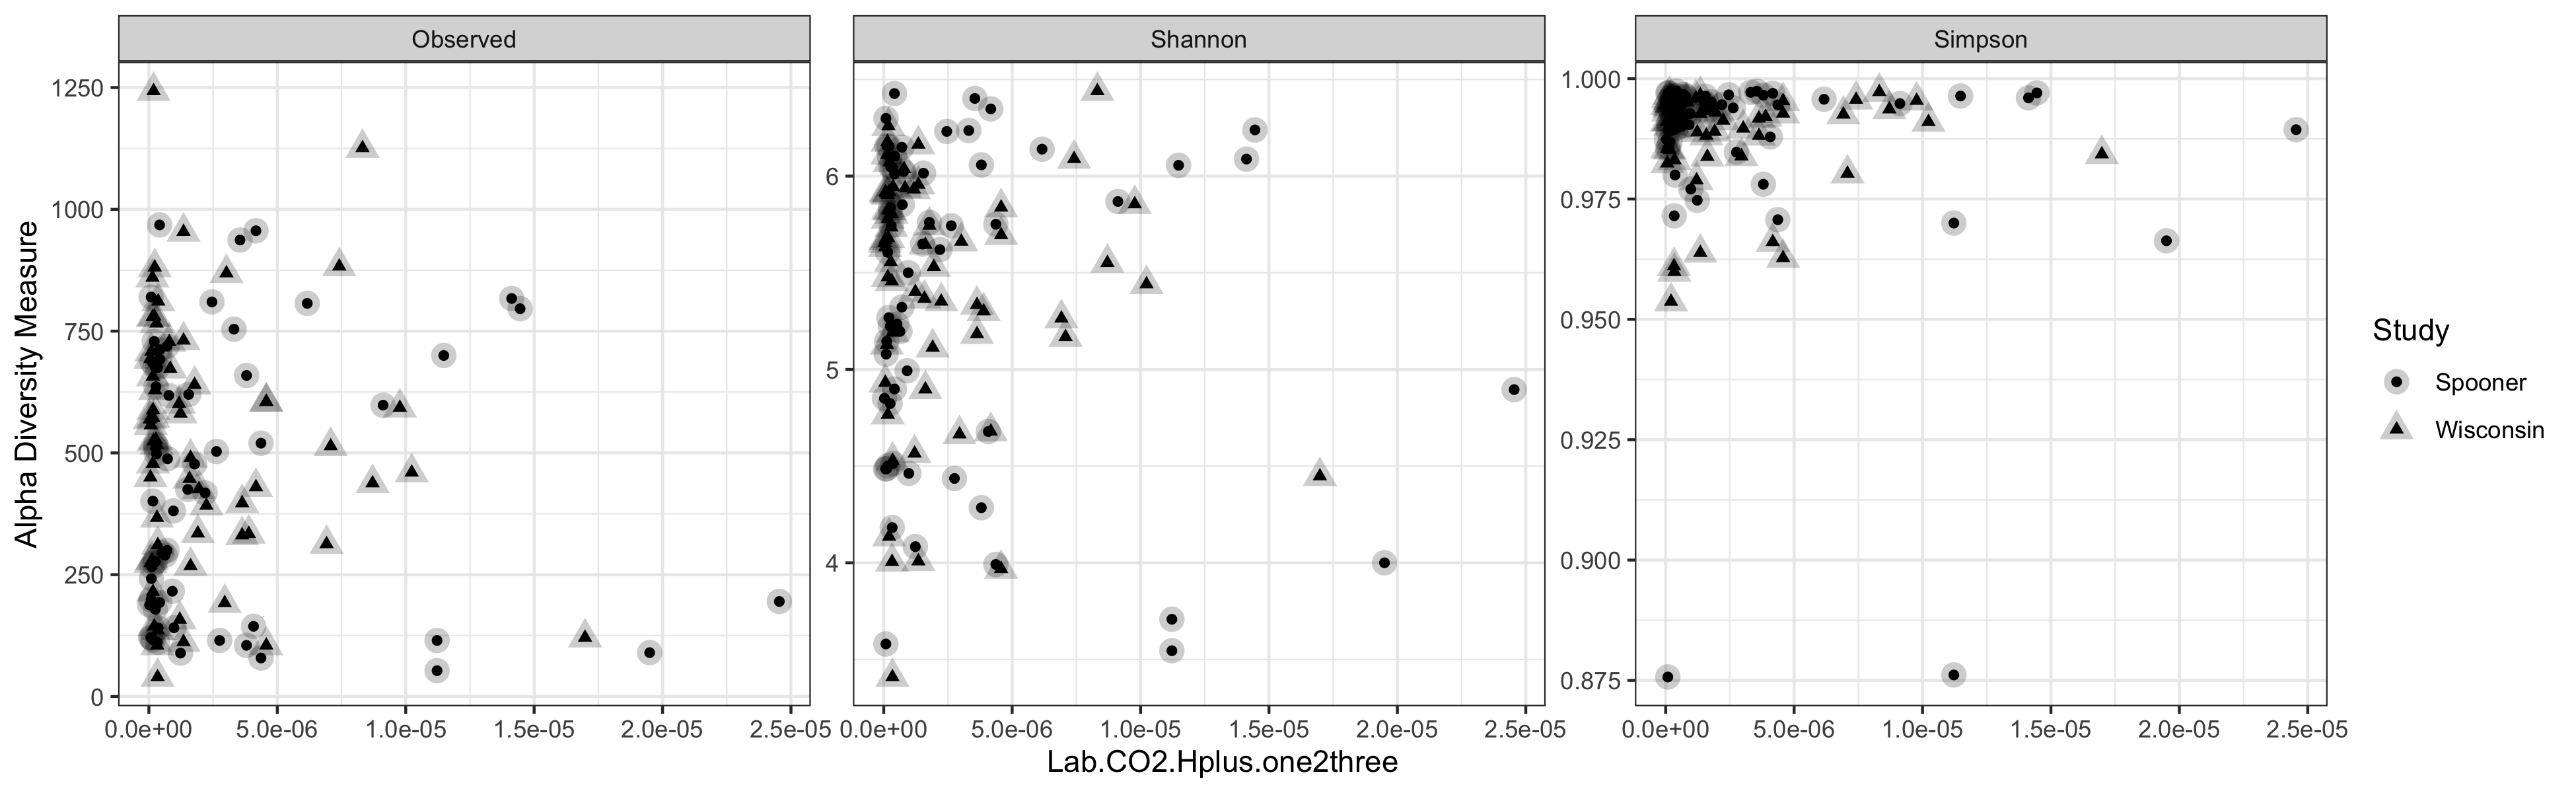
\includegraphics{output-rmd/richness-ph-Lab.CO2.Hplus.one2three-1.png}

\begin{Shaded}
\begin{Highlighting}[]
\NormalTok{p <-}\StringTok{ }\KeywordTok{plot_richness}\NormalTok{(ps, }\DataTypeTok{x=}\StringTok{"Lab.CO2.Hplus.one2four"}\NormalTok{, }\DataTypeTok{measures=}\KeywordTok{c}\NormalTok{(}\StringTok{"Observed"}\NormalTok{,}\StringTok{"Simpson"}\NormalTok{,}\StringTok{"Shannon"}\NormalTok{), }\DataTypeTok{scales =} \StringTok{"free_y"}\NormalTok{, }\DataTypeTok{shape=}\StringTok{"Study"}\NormalTok{)}
\NormalTok{p }\OperatorTok{+}\StringTok{ }\KeywordTok{geom_point}\NormalTok{(}\DataTypeTok{size=}\DecValTok{4}\NormalTok{, }\DataTypeTok{alpha=}\FloatTok{0.2}\NormalTok{) }\OperatorTok{+}\StringTok{ }\KeywordTok{theme_bw}\NormalTok{()}
\end{Highlighting}
\end{Shaded}

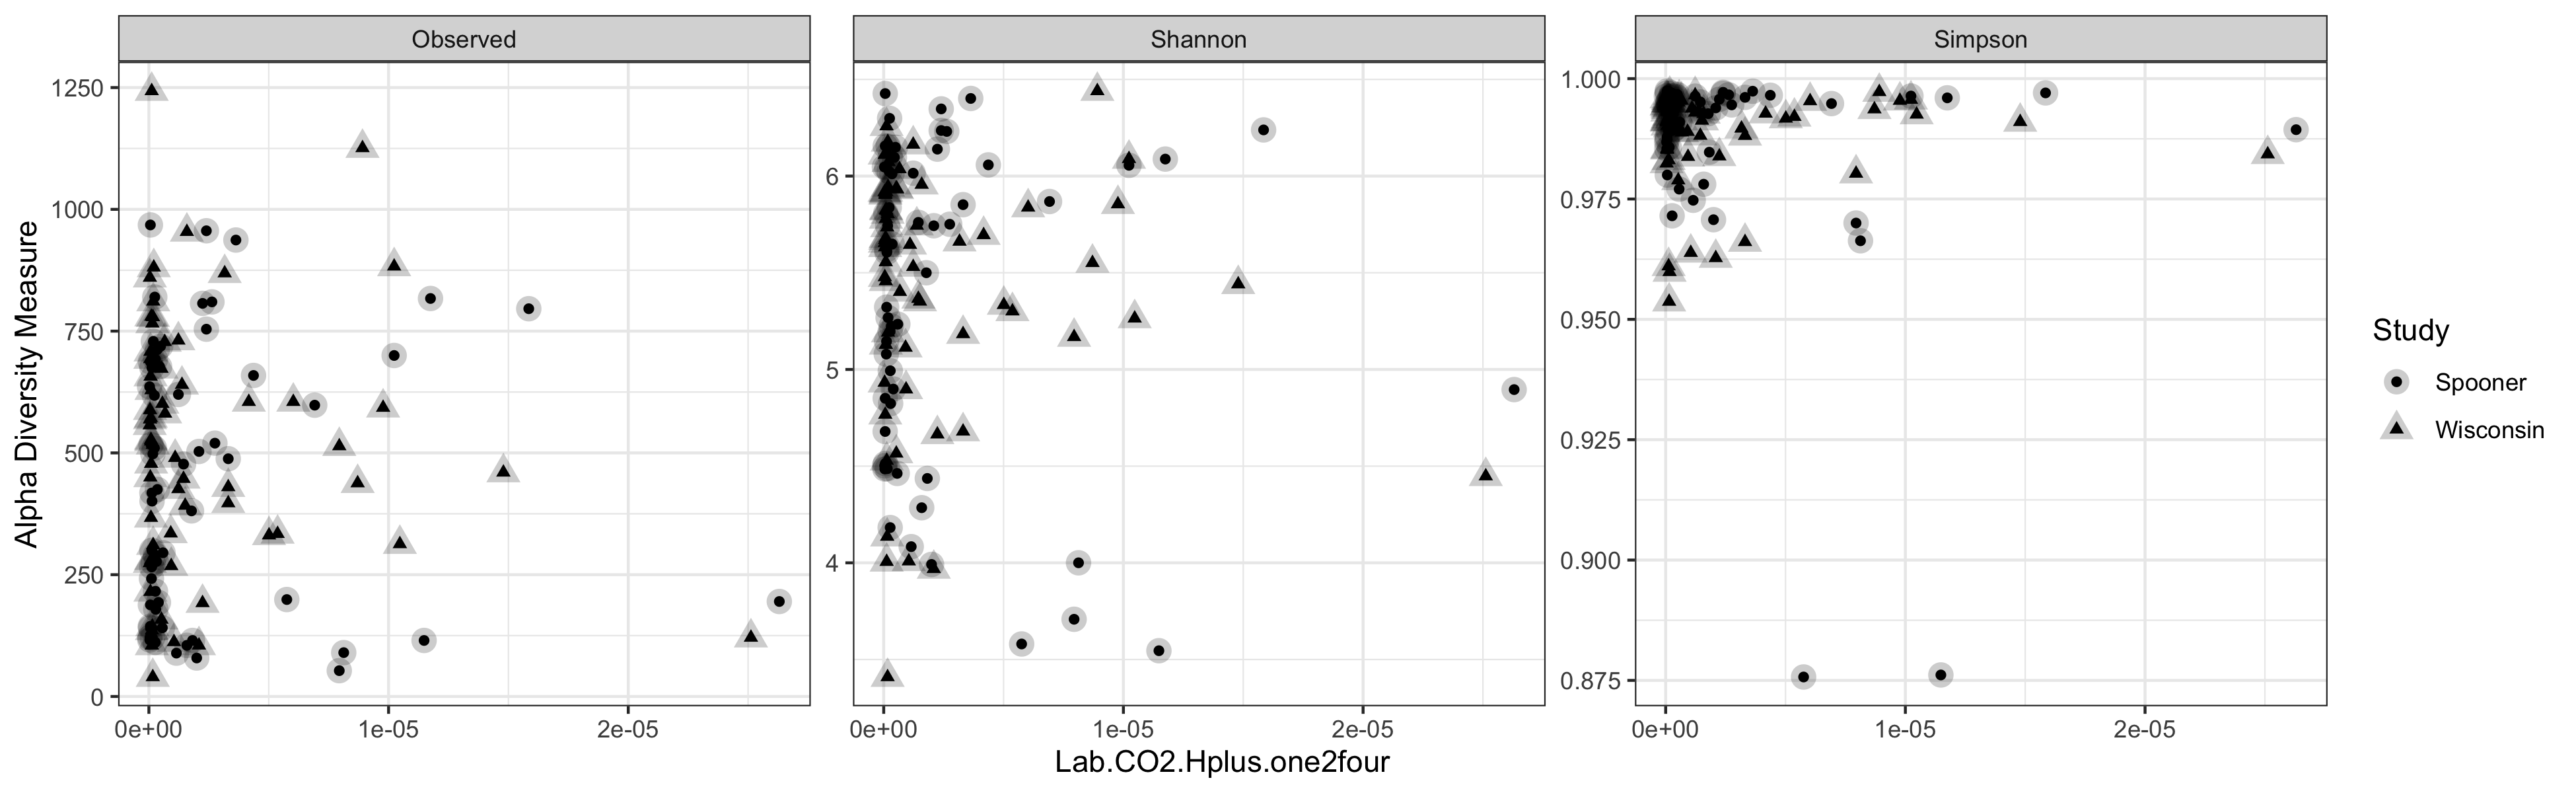
\includegraphics{output-rmd/richness-ph-Lab.CO2.Hplus.one2four-1.png}

\hypertarget{spooner-vs.-wisconsin}{%
\section{Spooner Vs. Wisconsin}\label{spooner-vs.-wisconsin}}

\begin{Shaded}
\begin{Highlighting}[]
\NormalTok{ps.wisc <-}\StringTok{ }\KeywordTok{subset_samples}\NormalTok{(ps, Study}\OperatorTok{==}\StringTok{"Wisconsin"}\NormalTok{)}
\NormalTok{ps.spoon <-}\StringTok{ }\KeywordTok{subset_samples}\NormalTok{(ps, Study}\OperatorTok{==}\StringTok{"Spooner"}\NormalTok{)}
\end{Highlighting}
\end{Shaded}

\begin{Shaded}
\begin{Highlighting}[]
\NormalTok{p.Lab.CO2.pH.one2one.wisc <-}\StringTok{ }\KeywordTok{plot_richness}\NormalTok{(ps.wisc, }\DataTypeTok{x=}\StringTok{"Lab.CO2.pH.one2one"}\NormalTok{, }\DataTypeTok{measures=}\KeywordTok{c}\NormalTok{(}\StringTok{"Observed"}\NormalTok{,}\StringTok{"Simpson"}\NormalTok{,}\StringTok{"Shannon"}\NormalTok{), }\DataTypeTok{scales =} \StringTok{"free_y"}\NormalTok{) }\OperatorTok{+}\StringTok{ }\KeywordTok{geom_point}\NormalTok{(}\DataTypeTok{size=}\DecValTok{4}\NormalTok{, }\DataTypeTok{alpha=}\FloatTok{0.2}\NormalTok{) }\OperatorTok{+}\StringTok{ }\KeywordTok{theme_bw}\NormalTok{() }\OperatorTok{+}\StringTok{ }\KeywordTok{labs}\NormalTok{(}\DataTypeTok{x =} \StringTok{"pH of Wisconsin Soils of 1:1 Water:Soil Ratio at approx. 400 ppm Carbon Dioxide"}\NormalTok{)}
\NormalTok{p.Lab.CO2.pH.one2one.wisc}
\end{Highlighting}
\end{Shaded}

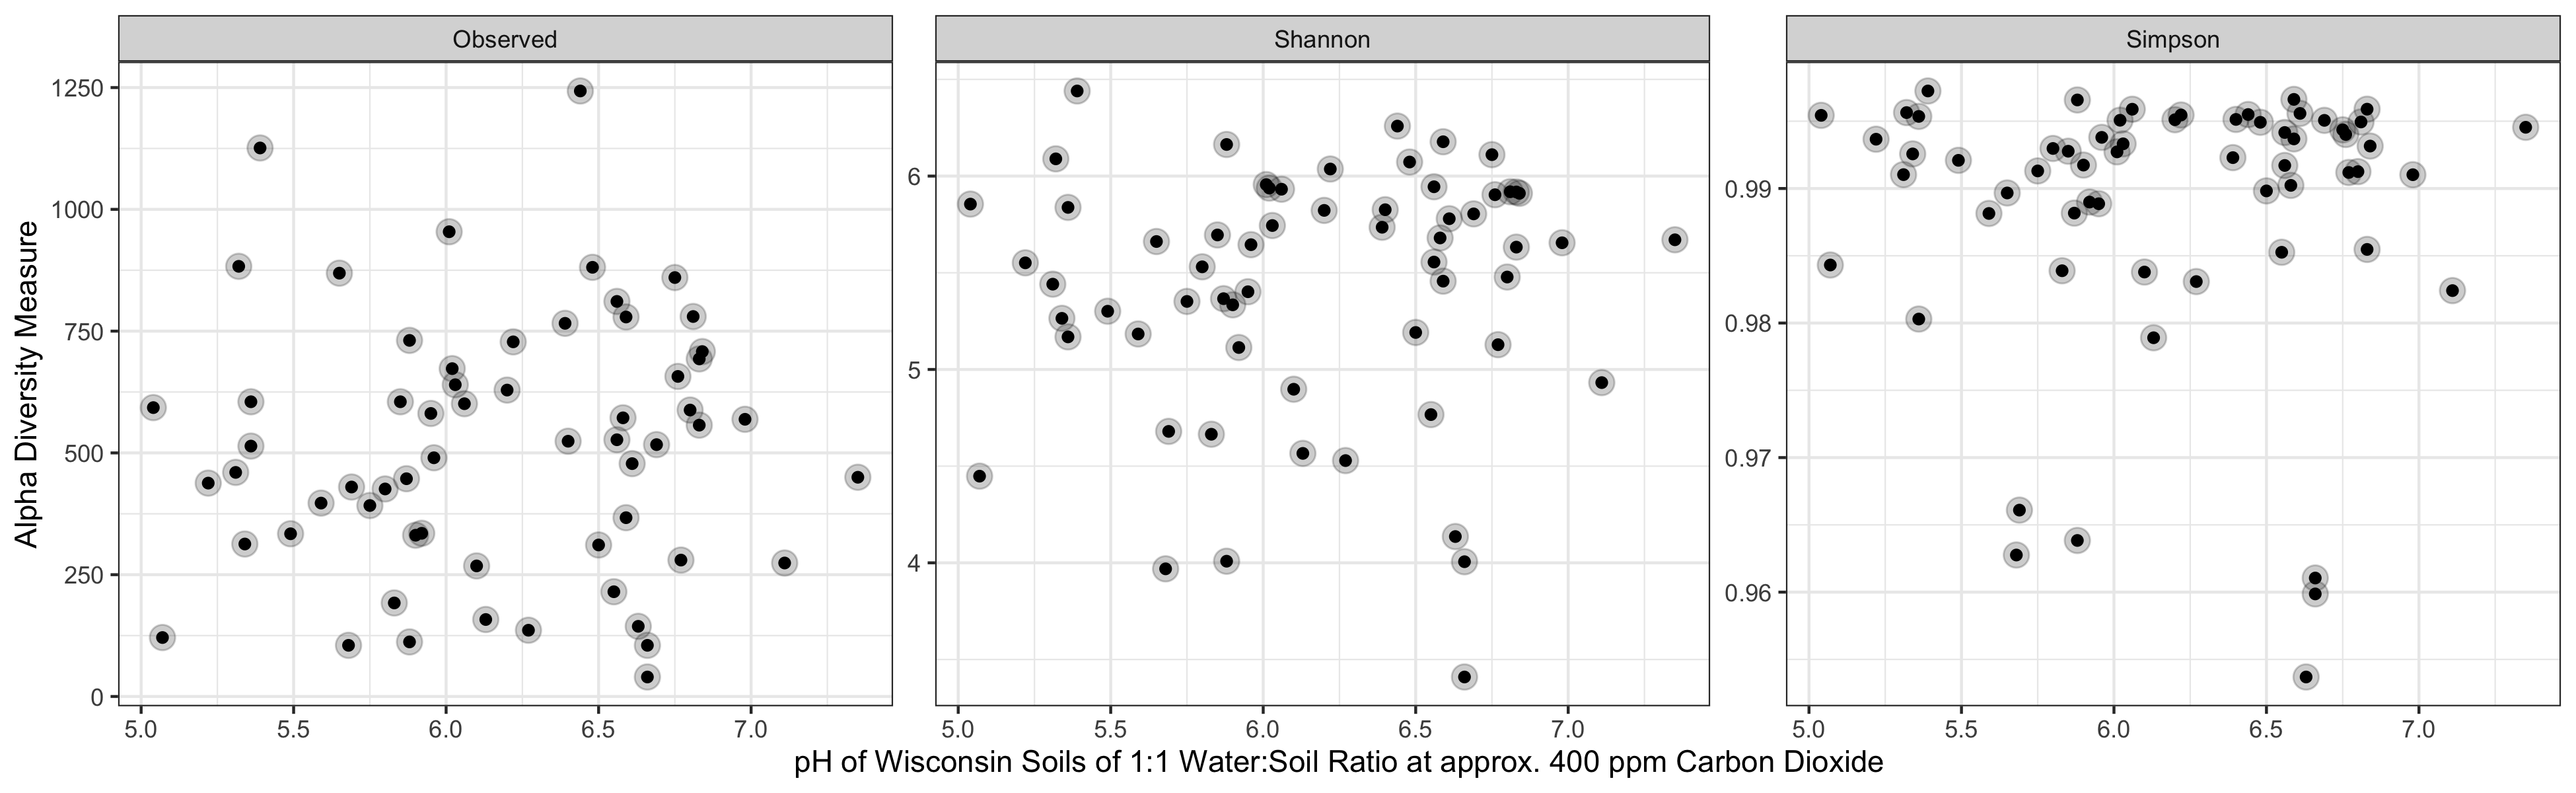
\includegraphics{output-rmd/richness-ph-Lab.CO2.pH.one2one.wisc-1.png}

\begin{Shaded}
\begin{Highlighting}[]
\NormalTok{p <-}\StringTok{ }\KeywordTok{plot_richness}\NormalTok{(ps.wisc, }\DataTypeTok{x=}\StringTok{"Lab.CO2.pH.one2two"}\NormalTok{, }\DataTypeTok{measures=}\KeywordTok{c}\NormalTok{(}\StringTok{"Observed"}\NormalTok{,}\StringTok{"Simpson"}\NormalTok{,}\StringTok{"Shannon"}\NormalTok{), }\DataTypeTok{scales =} \StringTok{"free_y"}\NormalTok{)}
\NormalTok{p }\OperatorTok{+}\StringTok{ }\KeywordTok{geom_point}\NormalTok{(}\DataTypeTok{size=}\DecValTok{4}\NormalTok{, }\DataTypeTok{alpha=}\FloatTok{0.2}\NormalTok{) }\OperatorTok{+}\StringTok{ }\KeywordTok{theme_bw}\NormalTok{()}
\end{Highlighting}
\end{Shaded}

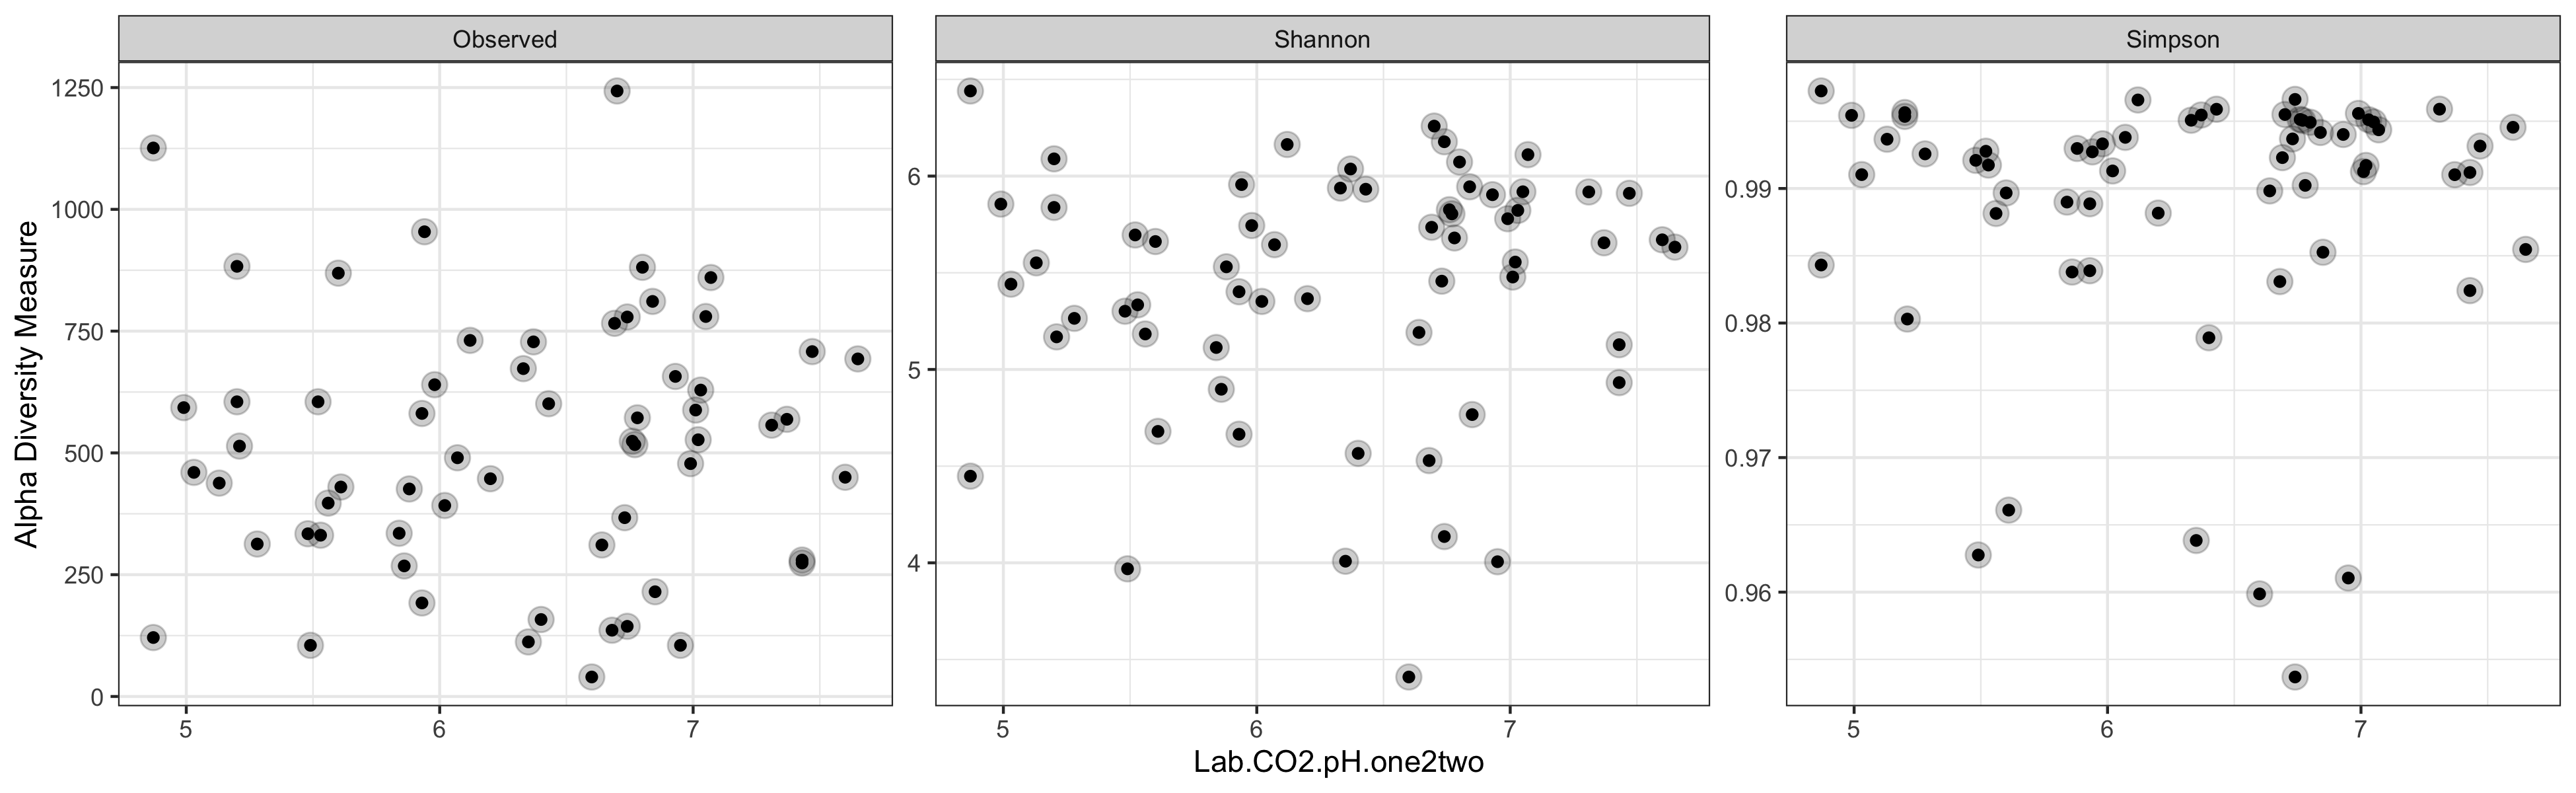
\includegraphics{output-rmd/richness-ph-Lab.CO2.pH.one2two.wisc-1.png}

\begin{Shaded}
\begin{Highlighting}[]
\NormalTok{p <-}\StringTok{ }\KeywordTok{plot_richness}\NormalTok{(ps.wisc, }\DataTypeTok{x=}\StringTok{"Lab.CO2.pH.one2three"}\NormalTok{, }\DataTypeTok{measures=}\KeywordTok{c}\NormalTok{(}\StringTok{"Observed"}\NormalTok{,}\StringTok{"Simpson"}\NormalTok{,}\StringTok{"Shannon"}\NormalTok{), }\DataTypeTok{scales =} \StringTok{"free_y"}\NormalTok{)}
\NormalTok{p }\OperatorTok{+}\StringTok{ }\KeywordTok{geom_point}\NormalTok{(}\DataTypeTok{size=}\DecValTok{4}\NormalTok{, }\DataTypeTok{alpha=}\FloatTok{0.2}\NormalTok{) }\OperatorTok{+}\StringTok{ }\KeywordTok{theme_bw}\NormalTok{()}
\end{Highlighting}
\end{Shaded}

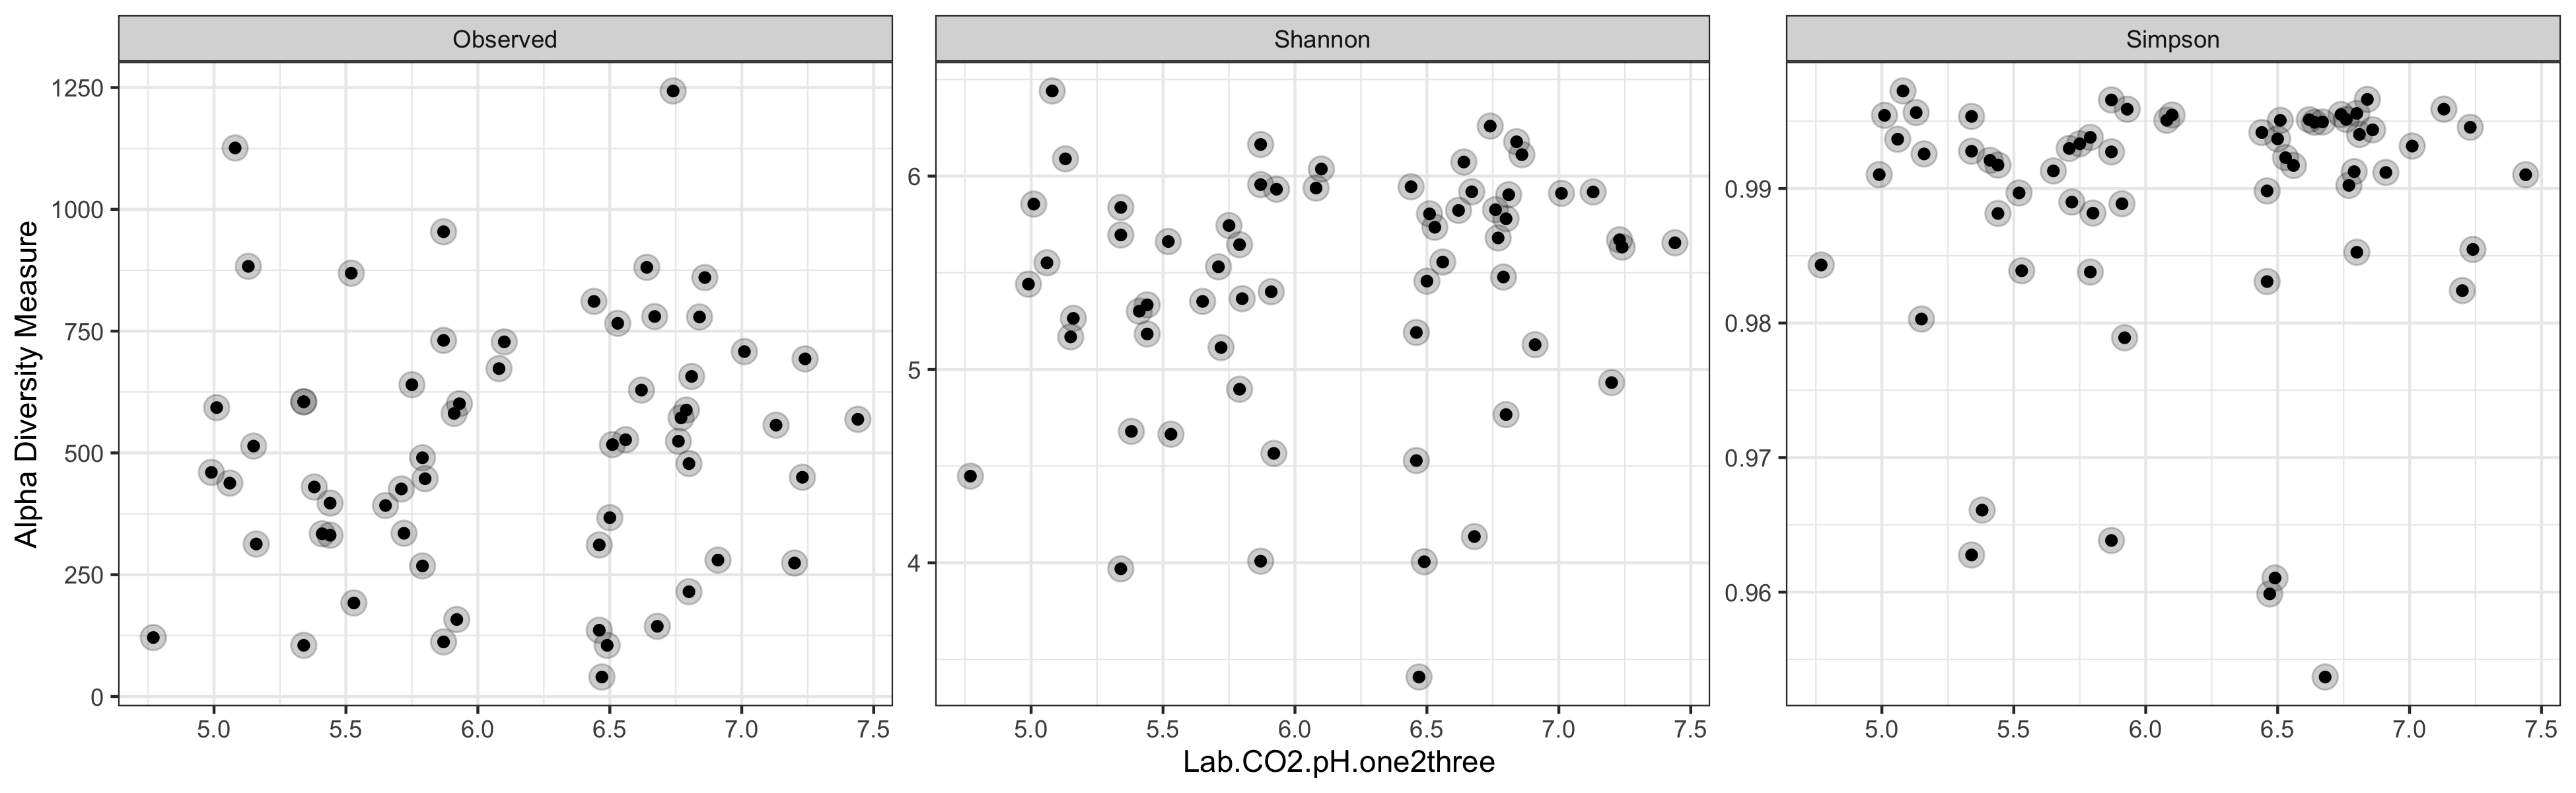
\includegraphics{output-rmd/richness-ph-Lab.CO2.pH.one2three.wisc-1.png}

\begin{Shaded}
\begin{Highlighting}[]
\NormalTok{p.Lab.CO2.pH.one2four.wisc <-}\StringTok{ }\KeywordTok{plot_richness}\NormalTok{(ps.wisc, }\DataTypeTok{x=}\StringTok{"Lab.CO2.pH.one2four"}\NormalTok{, }\DataTypeTok{measures=}\KeywordTok{c}\NormalTok{(}\StringTok{"Observed"}\NormalTok{,}\StringTok{"Simpson"}\NormalTok{,}\StringTok{"Shannon"}\NormalTok{), }\DataTypeTok{scales =} \StringTok{"free_y"}\NormalTok{) }\OperatorTok{+}\StringTok{ }\KeywordTok{geom_point}\NormalTok{(}\DataTypeTok{size=}\DecValTok{4}\NormalTok{, }\DataTypeTok{alpha=}\FloatTok{0.2}\NormalTok{) }\OperatorTok{+}\StringTok{ }\KeywordTok{theme_bw}\NormalTok{()  }\OperatorTok{+}\StringTok{ }\KeywordTok{labs}\NormalTok{(}\DataTypeTok{x =} \StringTok{"pH of Wisconsin Soils of 1:4 Water:Soil Ratio at approx. 400 ppm Carbon Dioxide"}\NormalTok{)}
\NormalTok{p.Lab.CO2.pH.one2four.wisc}
\end{Highlighting}
\end{Shaded}

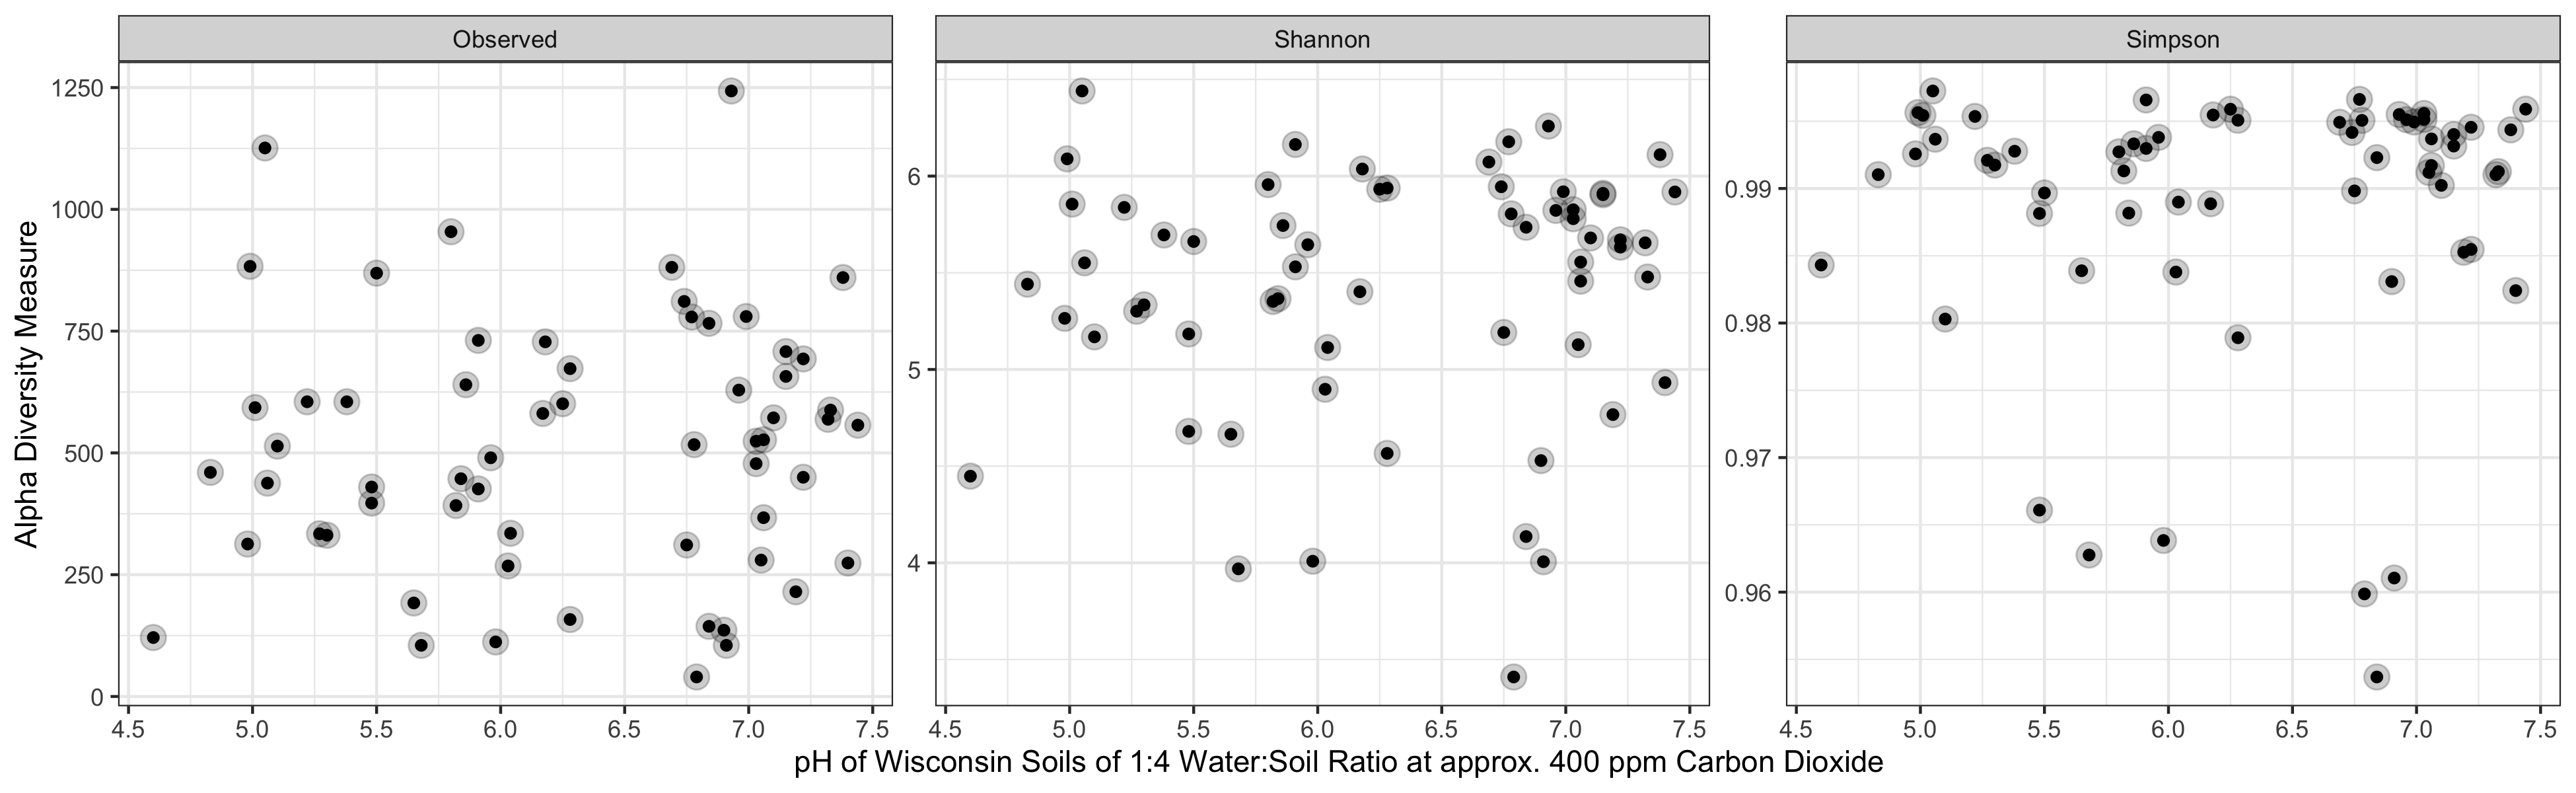
\includegraphics{output-rmd/richness-ph-Lab.CO2.pH.one2four.wisc-1.png}

\begin{Shaded}
\begin{Highlighting}[]
\NormalTok{p <-}\StringTok{ }\KeywordTok{plot_richness}\NormalTok{(ps.wisc, }\DataTypeTok{x=}\StringTok{"Lab.CO2.Hplus.one2one"}\NormalTok{, }\DataTypeTok{measures=}\KeywordTok{c}\NormalTok{(}\StringTok{"Observed"}\NormalTok{,}\StringTok{"Simpson"}\NormalTok{,}\StringTok{"Shannon"}\NormalTok{), }\DataTypeTok{scales =} \StringTok{"free_y"}\NormalTok{)}
\NormalTok{p }\OperatorTok{+}\StringTok{ }\KeywordTok{geom_point}\NormalTok{(}\DataTypeTok{size=}\DecValTok{4}\NormalTok{, }\DataTypeTok{alpha=}\FloatTok{0.2}\NormalTok{) }\OperatorTok{+}\StringTok{ }\KeywordTok{theme_bw}\NormalTok{()}
\end{Highlighting}
\end{Shaded}

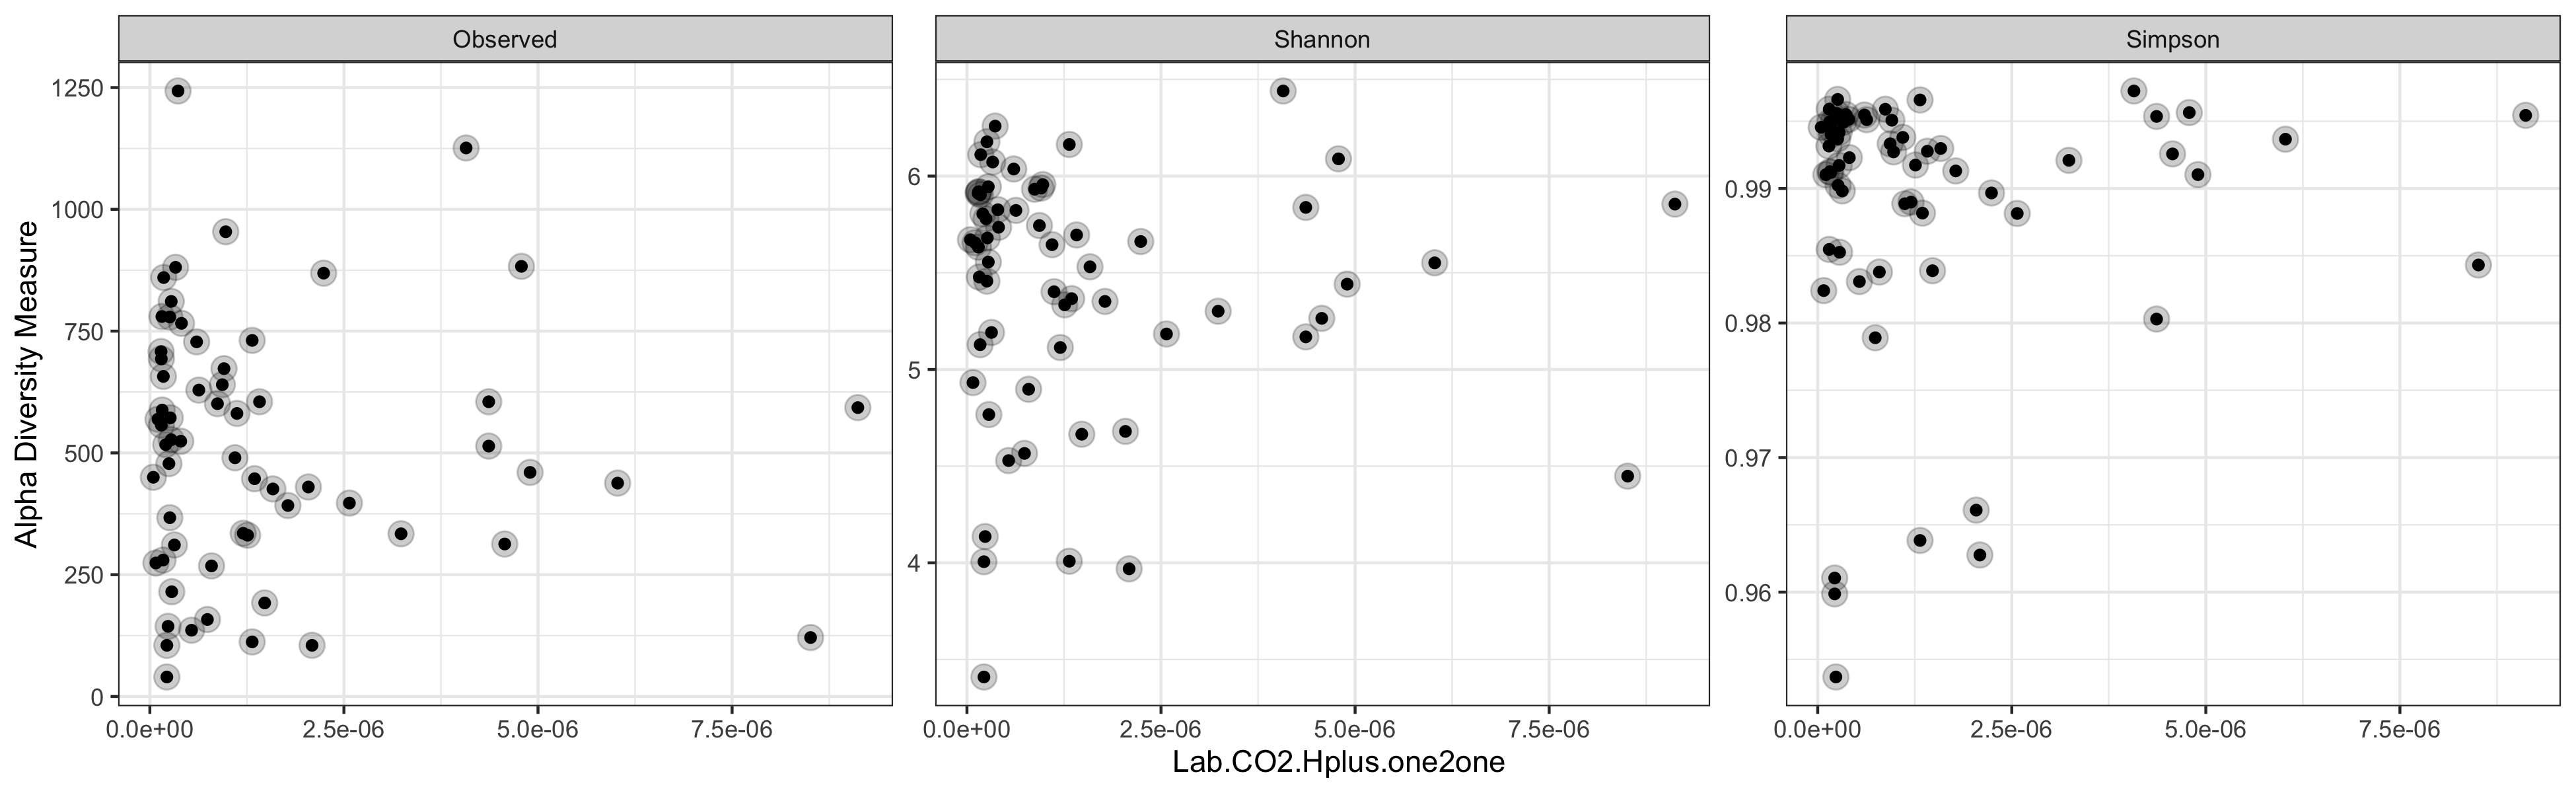
\includegraphics{output-rmd/richness-ph-Lab.CO2.Hplus.one2one.wisc-1.png}

\begin{Shaded}
\begin{Highlighting}[]
\NormalTok{p <-}\StringTok{ }\KeywordTok{plot_richness}\NormalTok{(ps.wisc, }\DataTypeTok{x=}\StringTok{"Lab.CO2.Hplus.one2two"}\NormalTok{, }\DataTypeTok{measures=}\KeywordTok{c}\NormalTok{(}\StringTok{"Observed"}\NormalTok{,}\StringTok{"Simpson"}\NormalTok{,}\StringTok{"Shannon"}\NormalTok{), }\DataTypeTok{scales =} \StringTok{"free_y"}\NormalTok{)}
\NormalTok{p }\OperatorTok{+}\StringTok{ }\KeywordTok{geom_point}\NormalTok{(}\DataTypeTok{size=}\DecValTok{4}\NormalTok{, }\DataTypeTok{alpha=}\FloatTok{0.2}\NormalTok{) }\OperatorTok{+}\StringTok{ }\KeywordTok{theme_bw}\NormalTok{()}
\end{Highlighting}
\end{Shaded}

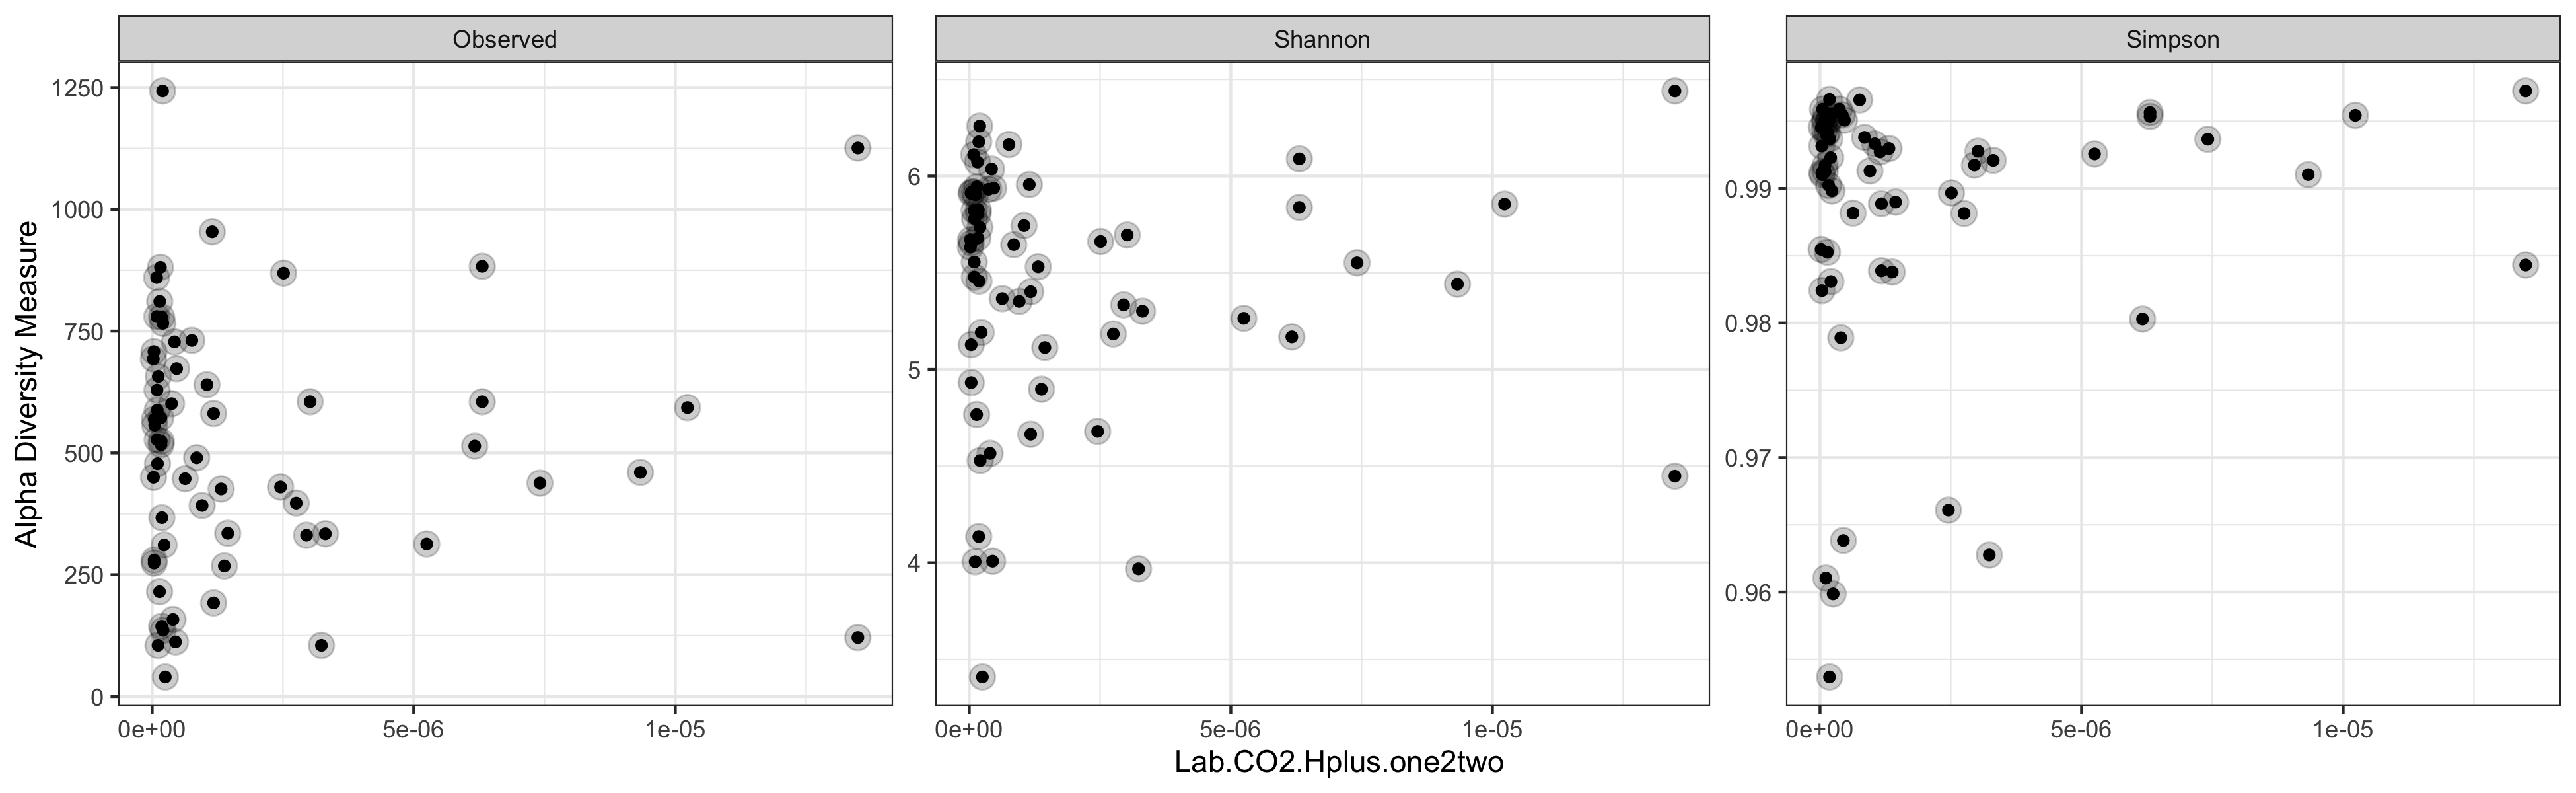
\includegraphics{output-rmd/richness-ph-Lab.CO2.Hplus.one2two.wisc-1.png}

\begin{Shaded}
\begin{Highlighting}[]
\NormalTok{p <-}\StringTok{ }\KeywordTok{plot_richness}\NormalTok{(ps.wisc, }\DataTypeTok{x=}\StringTok{"Lab.CO2.Hplus.one2three"}\NormalTok{, }\DataTypeTok{measures=}\KeywordTok{c}\NormalTok{(}\StringTok{"Observed"}\NormalTok{,}\StringTok{"Simpson"}\NormalTok{,}\StringTok{"Shannon"}\NormalTok{), }\DataTypeTok{scales =} \StringTok{"free_y"}\NormalTok{)}
\NormalTok{p }\OperatorTok{+}\StringTok{ }\KeywordTok{geom_point}\NormalTok{(}\DataTypeTok{size=}\DecValTok{4}\NormalTok{, }\DataTypeTok{alpha=}\FloatTok{0.2}\NormalTok{) }\OperatorTok{+}\StringTok{ }\KeywordTok{theme_bw}\NormalTok{()}
\end{Highlighting}
\end{Shaded}

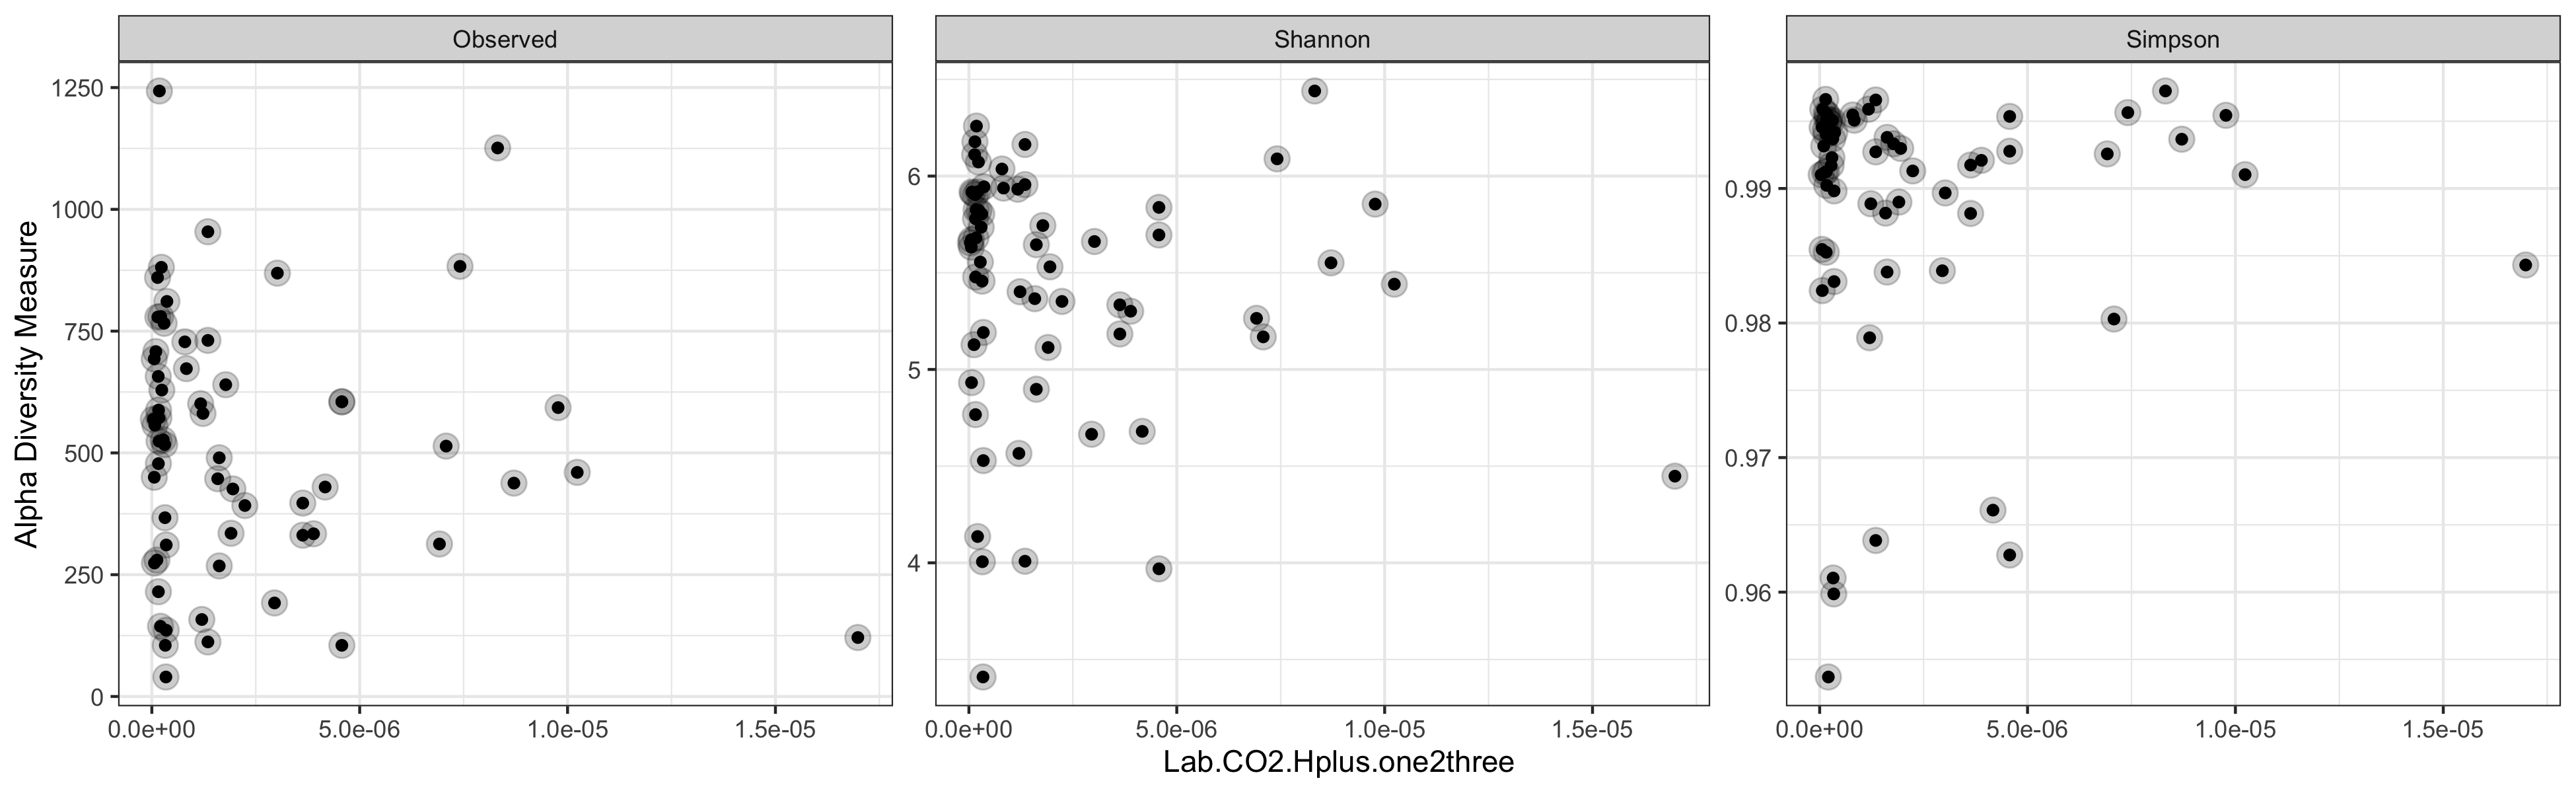
\includegraphics{output-rmd/richness-ph-Lab.CO2.Hplus.one2three.wisc-1.png}

\begin{Shaded}
\begin{Highlighting}[]
\NormalTok{p <-}\StringTok{ }\KeywordTok{plot_richness}\NormalTok{(ps.wisc, }\DataTypeTok{x=}\StringTok{"Lab.CO2.Hplus.one2four"}\NormalTok{, }\DataTypeTok{measures=}\KeywordTok{c}\NormalTok{(}\StringTok{"Observed"}\NormalTok{,}\StringTok{"Simpson"}\NormalTok{,}\StringTok{"Shannon"}\NormalTok{), }\DataTypeTok{scales =} \StringTok{"free_y"}\NormalTok{)}
\NormalTok{p }\OperatorTok{+}\StringTok{ }\KeywordTok{geom_point}\NormalTok{(}\DataTypeTok{size=}\DecValTok{4}\NormalTok{, }\DataTypeTok{alpha=}\FloatTok{0.2}\NormalTok{) }\OperatorTok{+}\StringTok{ }\KeywordTok{theme_bw}\NormalTok{()}
\end{Highlighting}
\end{Shaded}

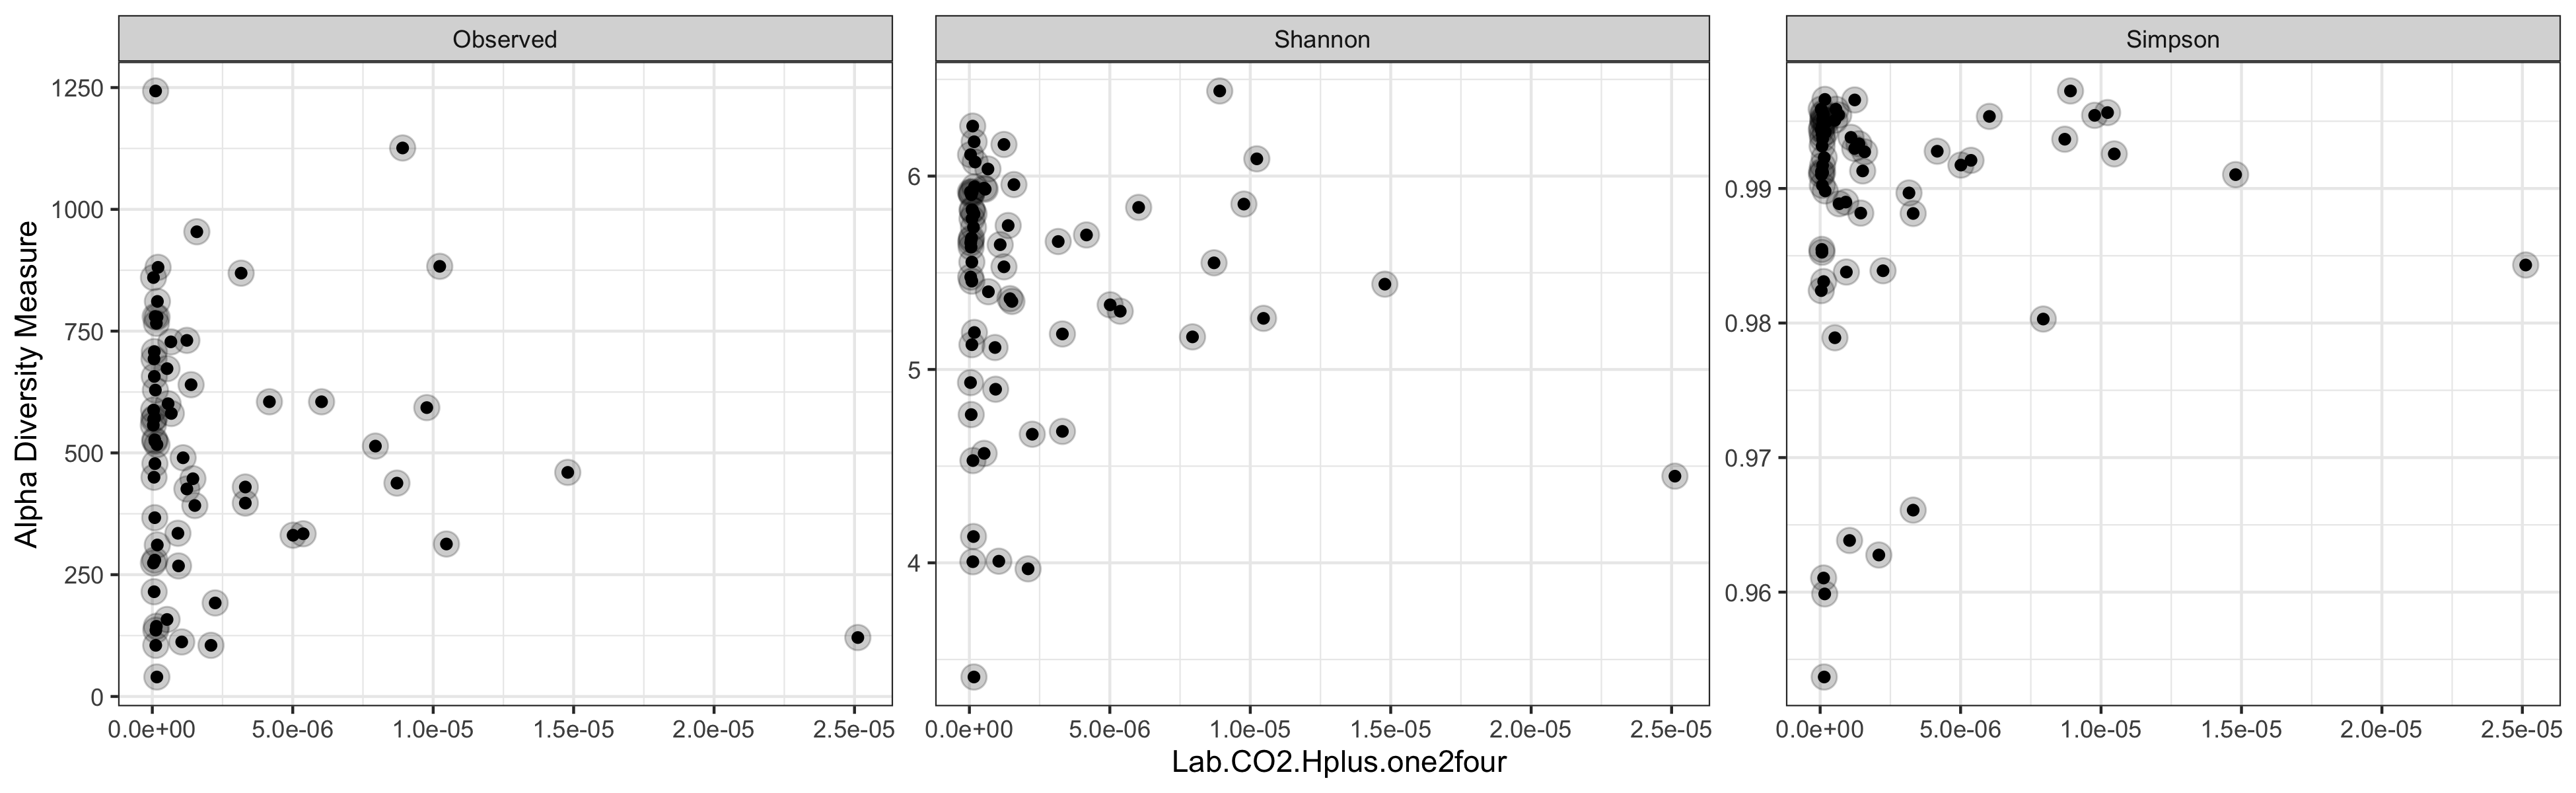
\includegraphics{output-rmd/richness-ph-Lab.CO2.Hplus.one2four.wisc-1.png}

\begin{Shaded}
\begin{Highlighting}[]
\NormalTok{p.Lab.CO2.pH.one2one.spoon <-}\StringTok{ }\KeywordTok{plot_richness}\NormalTok{(ps.spoon, }\DataTypeTok{x=}\StringTok{"Lab.CO2.pH.one2one"}\NormalTok{, }\DataTypeTok{measures=}\KeywordTok{c}\NormalTok{(}\StringTok{"Observed"}\NormalTok{,}\StringTok{"Simpson"}\NormalTok{,}\StringTok{"Shannon"}\NormalTok{), }\DataTypeTok{scales =} \StringTok{"free_y"}\NormalTok{) }\OperatorTok{+}\StringTok{ }\KeywordTok{geom_point}\NormalTok{(}\DataTypeTok{size=}\DecValTok{4}\NormalTok{, }\DataTypeTok{alpha=}\FloatTok{0.2}\NormalTok{) }\OperatorTok{+}\StringTok{ }\KeywordTok{theme_bw}\NormalTok{() }\OperatorTok{+}\StringTok{ }\KeywordTok{labs}\NormalTok{(}\DataTypeTok{x =} \StringTok{"pH of Spooner Soils of 1:1 Water:Soil Ratio at approx. 400 ppm Carbon Dioxide"}\NormalTok{)}
\NormalTok{p.Lab.CO2.pH.one2one.spoon}
\end{Highlighting}
\end{Shaded}

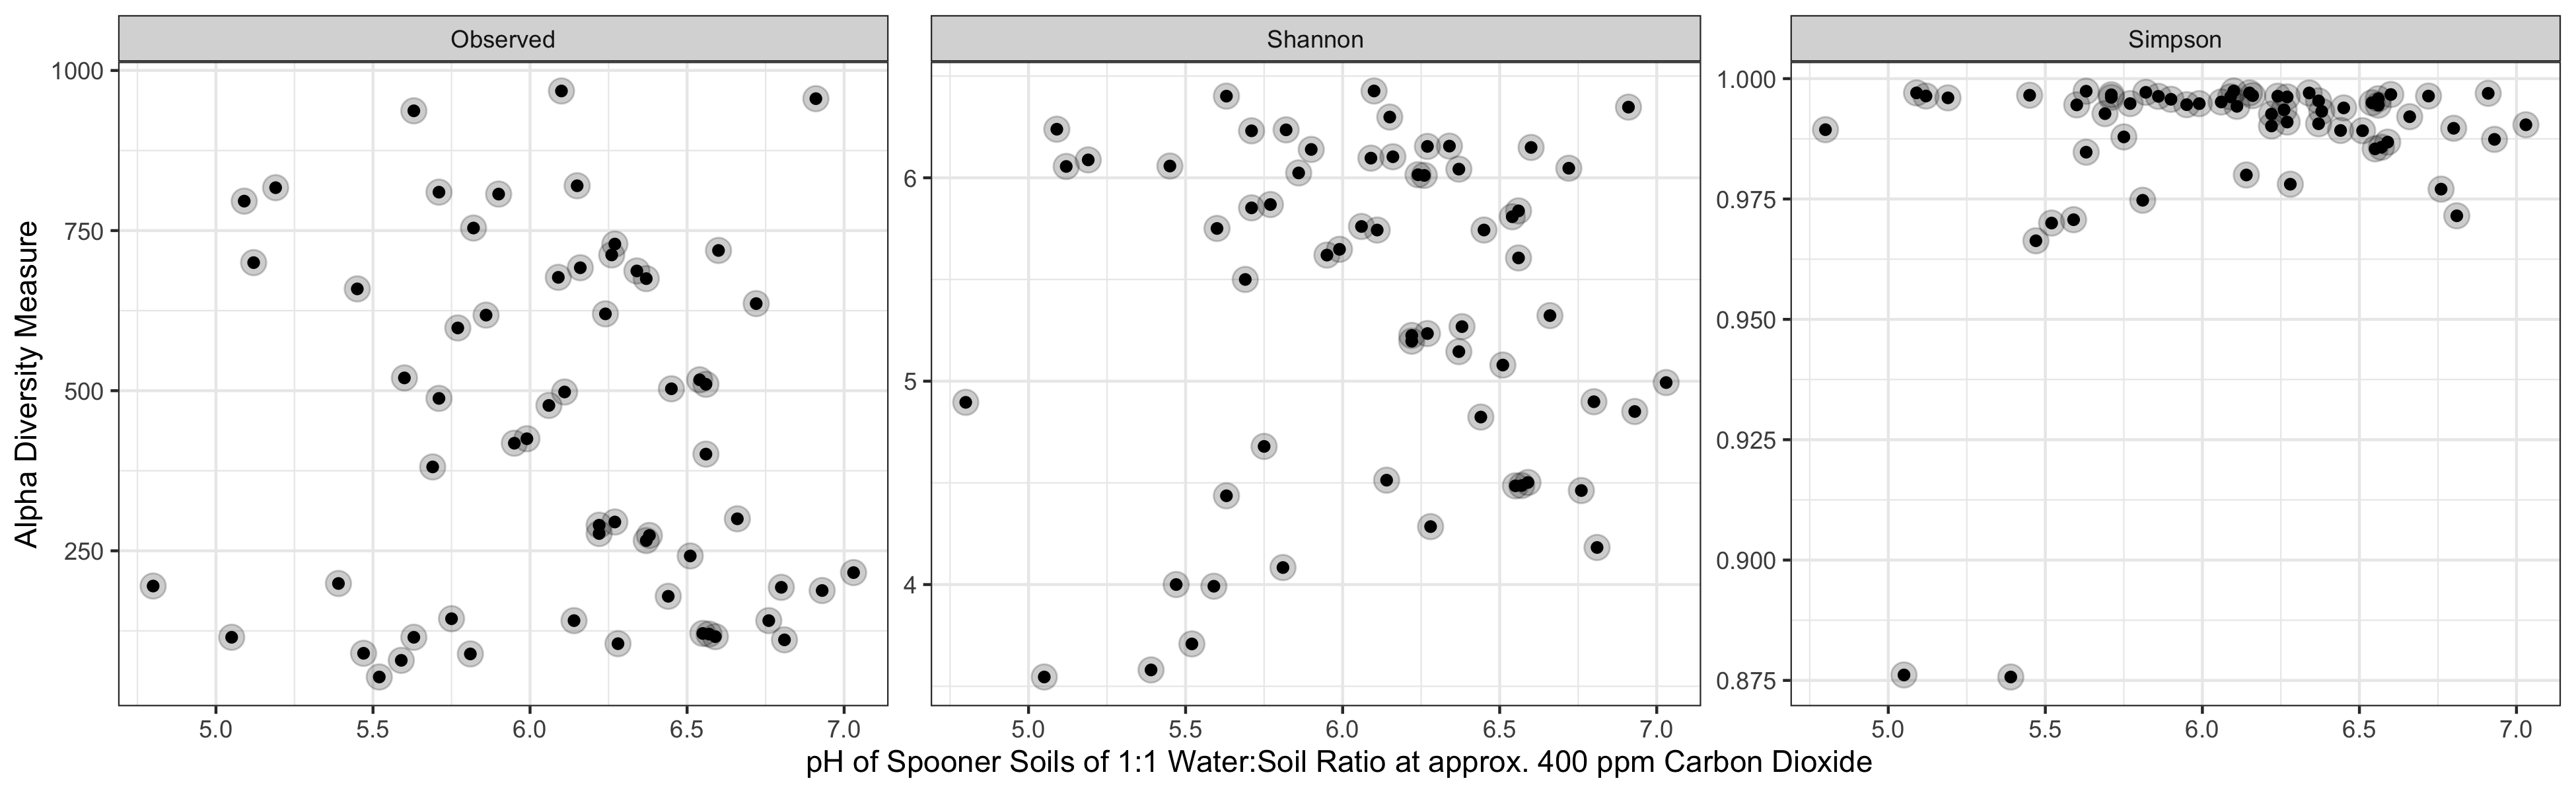
\includegraphics{output-rmd/richness-ph-Lab.CO2.pH.one2one.spoon-1.png}

\begin{Shaded}
\begin{Highlighting}[]
\NormalTok{p <-}\StringTok{ }\KeywordTok{plot_richness}\NormalTok{(ps.spoon, }\DataTypeTok{x=}\StringTok{"Lab.CO2.pH.one2two"}\NormalTok{, }\DataTypeTok{measures=}\KeywordTok{c}\NormalTok{(}\StringTok{"Observed"}\NormalTok{,}\StringTok{"Simpson"}\NormalTok{,}\StringTok{"Shannon"}\NormalTok{), }\DataTypeTok{scales =} \StringTok{"free_y"}\NormalTok{)}
\NormalTok{p }\OperatorTok{+}\StringTok{ }\KeywordTok{geom_point}\NormalTok{(}\DataTypeTok{size=}\DecValTok{4}\NormalTok{, }\DataTypeTok{alpha=}\FloatTok{0.2}\NormalTok{) }\OperatorTok{+}\StringTok{ }\KeywordTok{theme_bw}\NormalTok{()}
\end{Highlighting}
\end{Shaded}

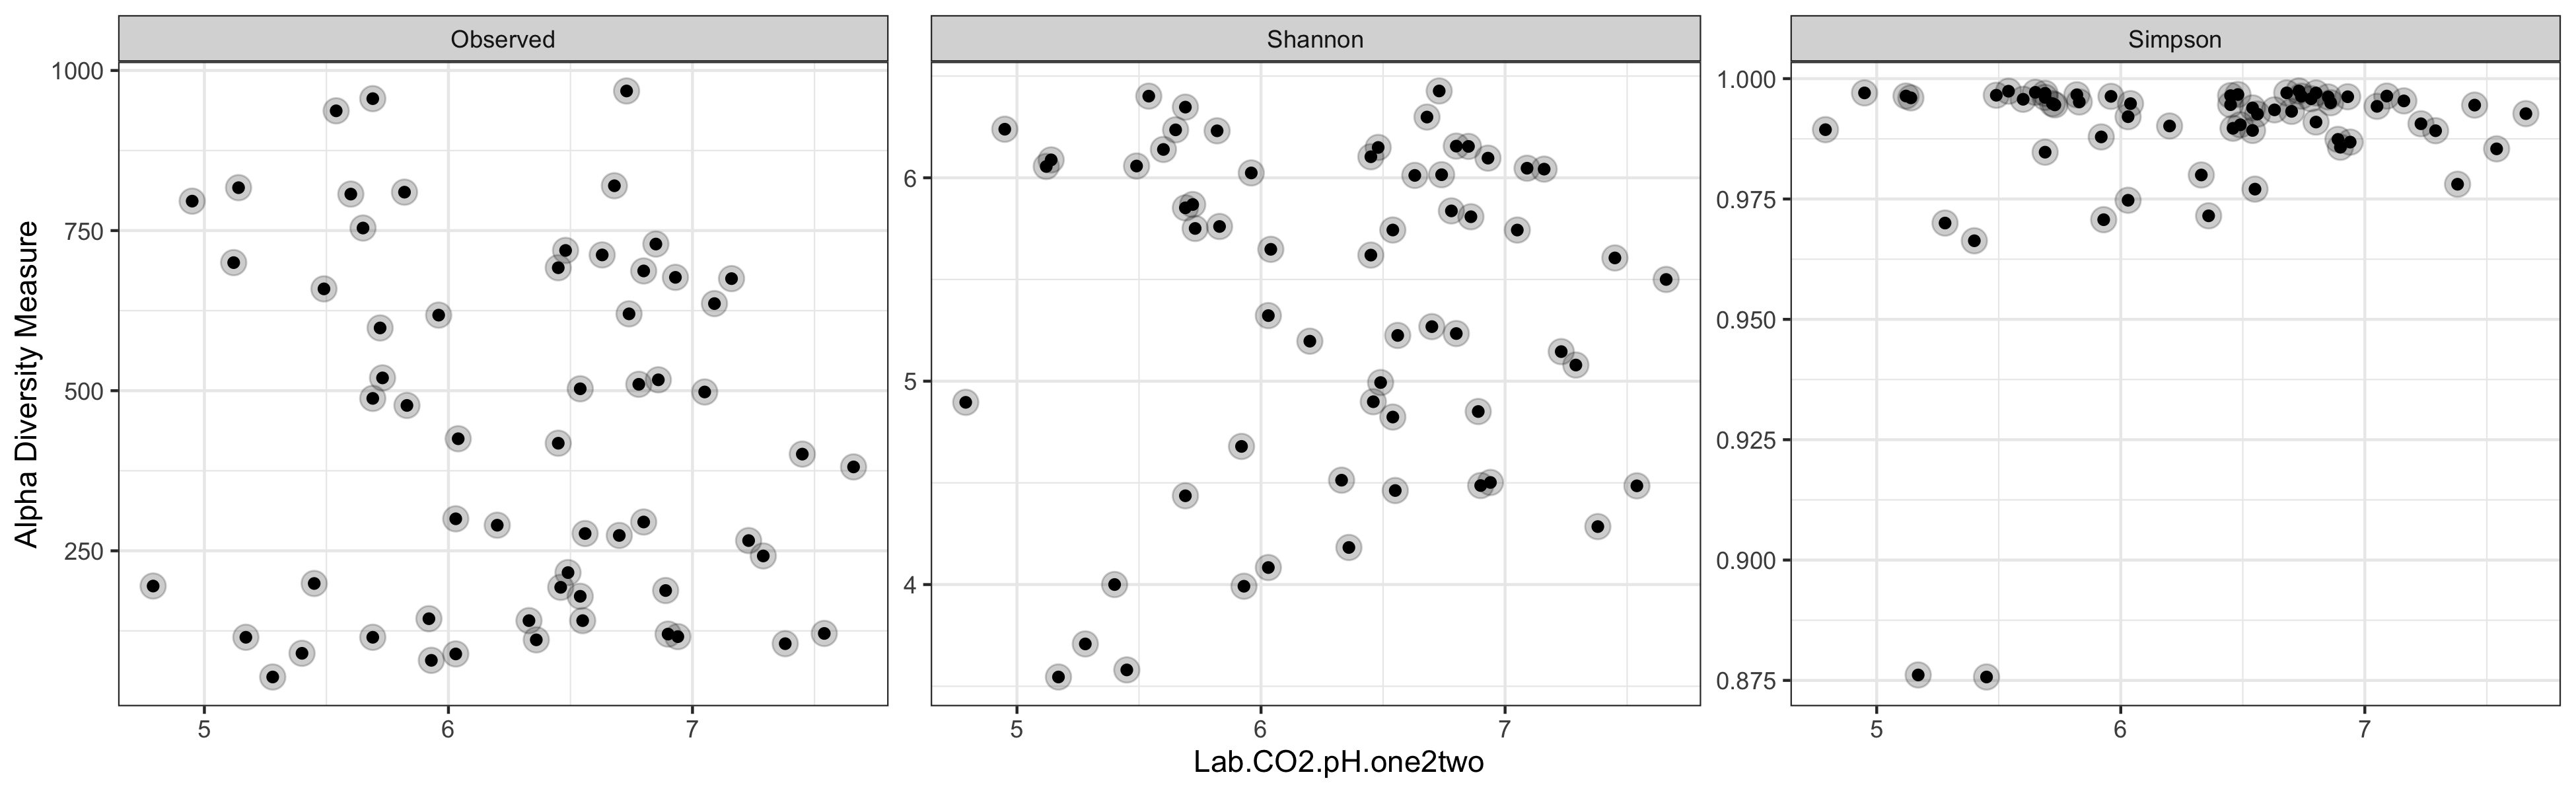
\includegraphics{output-rmd/richness-ph-Lab.CO2.pH.one2two.spoon-1.png}

\begin{Shaded}
\begin{Highlighting}[]
\NormalTok{p <-}\StringTok{ }\KeywordTok{plot_richness}\NormalTok{(ps.spoon, }\DataTypeTok{x=}\StringTok{"Lab.CO2.pH.one2three"}\NormalTok{, }\DataTypeTok{measures=}\KeywordTok{c}\NormalTok{(}\StringTok{"Observed"}\NormalTok{,}\StringTok{"Simpson"}\NormalTok{,}\StringTok{"Shannon"}\NormalTok{), }\DataTypeTok{scales =} \StringTok{"free_y"}\NormalTok{)}
\NormalTok{p }\OperatorTok{+}\StringTok{ }\KeywordTok{geom_point}\NormalTok{(}\DataTypeTok{size=}\DecValTok{4}\NormalTok{, }\DataTypeTok{alpha=}\FloatTok{0.2}\NormalTok{) }\OperatorTok{+}\StringTok{ }\KeywordTok{theme_bw}\NormalTok{()}
\end{Highlighting}
\end{Shaded}

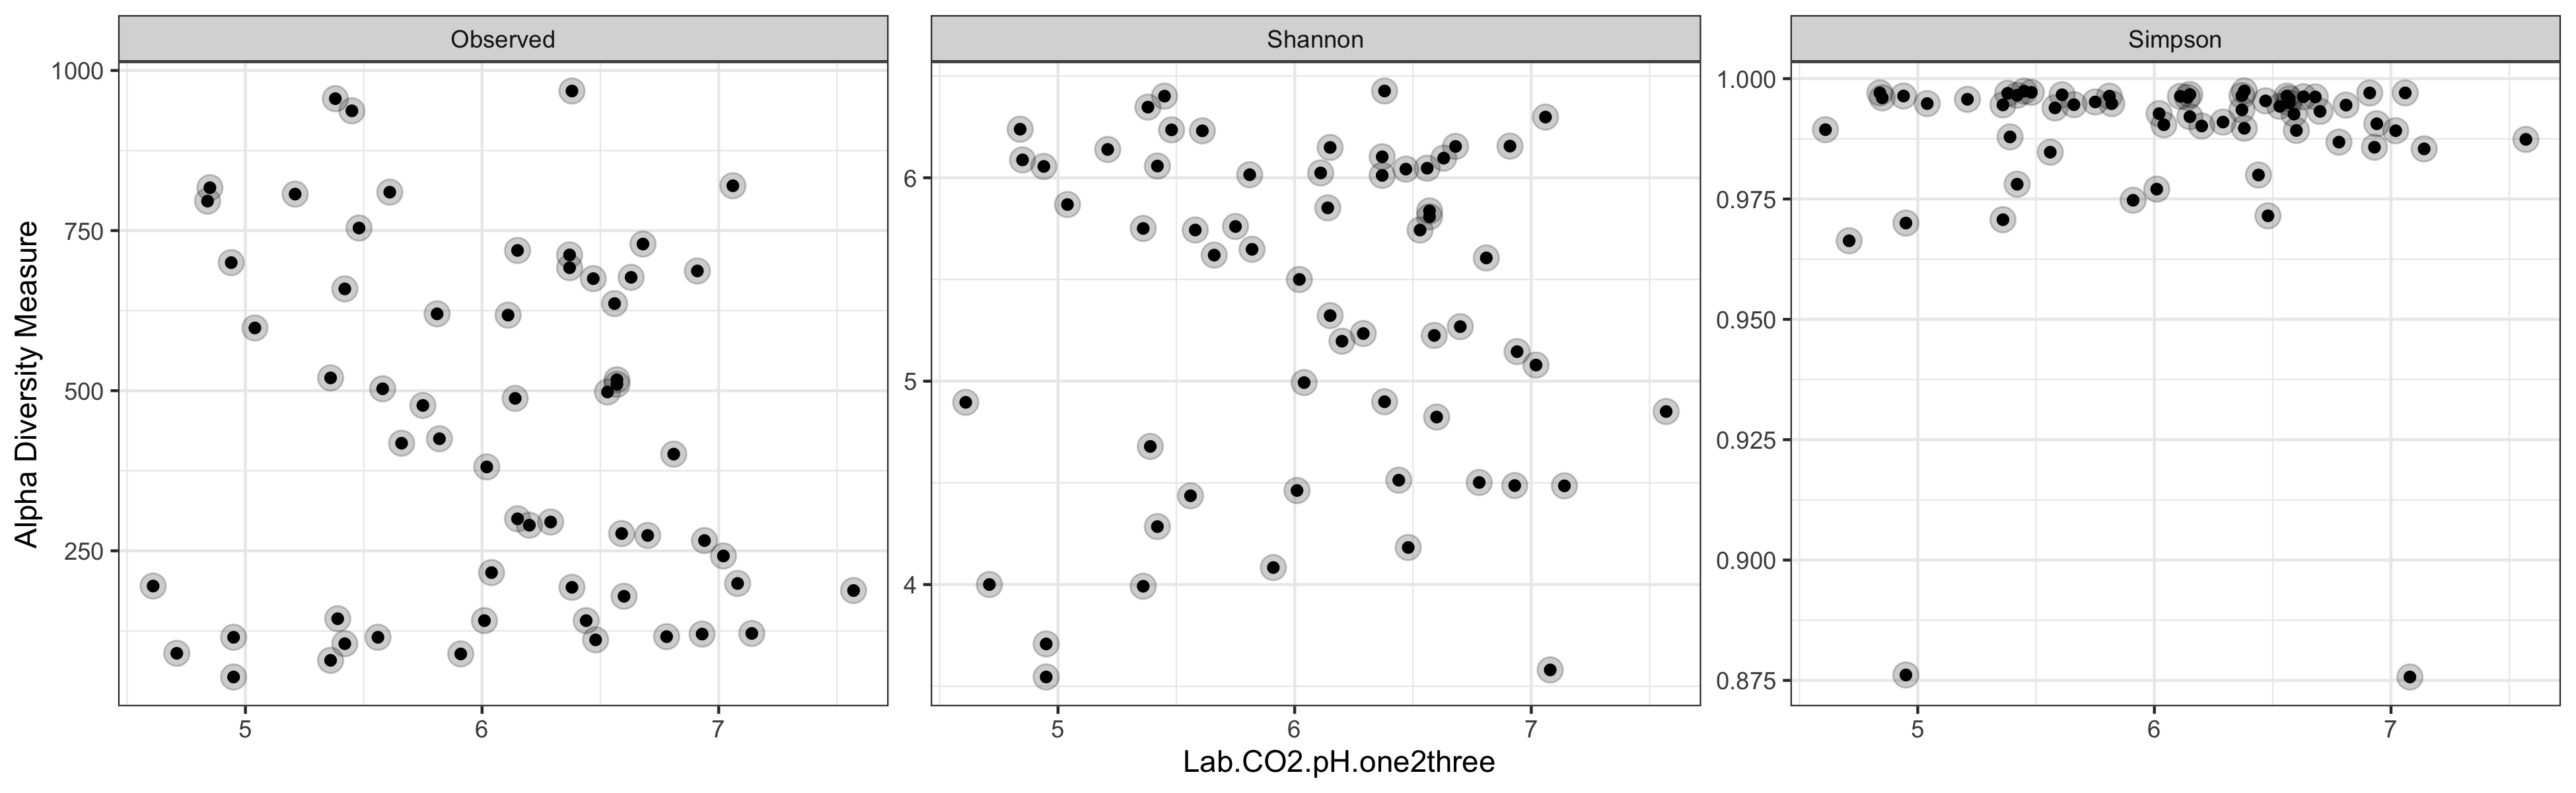
\includegraphics{output-rmd/richness-ph-Lab.CO2.pH.one2three.spoon-1.png}

\begin{Shaded}
\begin{Highlighting}[]
\NormalTok{p.Lab.CO2.pH.one2four.spoon <-}\StringTok{ }\KeywordTok{plot_richness}\NormalTok{(ps.spoon, }\DataTypeTok{x=}\StringTok{"Lab.CO2.pH.one2four"}\NormalTok{, }\DataTypeTok{measures=}\KeywordTok{c}\NormalTok{(}\StringTok{"Observed"}\NormalTok{,}\StringTok{"Simpson"}\NormalTok{,}\StringTok{"Shannon"}\NormalTok{), }\DataTypeTok{scales =} \StringTok{"free_y"}\NormalTok{) }\OperatorTok{+}\StringTok{ }\KeywordTok{geom_point}\NormalTok{(}\DataTypeTok{size=}\DecValTok{4}\NormalTok{, }\DataTypeTok{alpha=}\FloatTok{0.2}\NormalTok{) }\OperatorTok{+}\StringTok{ }\KeywordTok{theme_bw}\NormalTok{() }\OperatorTok{+}\StringTok{ }\KeywordTok{labs}\NormalTok{(}\DataTypeTok{x =} \StringTok{"pH of Spooner Soils of 1:4 Water:Soil Ratio at approx. 400 ppm Carbon Dioxide"}\NormalTok{)}
\NormalTok{p.Lab.CO2.pH.one2four.spoon}
\end{Highlighting}
\end{Shaded}

\includegraphics{output-rmd/richness-ph-Lab.CO2.pH.one2four.spoon-1.png}

\begin{Shaded}
\begin{Highlighting}[]
\NormalTok{p <-}\StringTok{ }\KeywordTok{plot_richness}\NormalTok{(ps.spoon, }\DataTypeTok{x=}\StringTok{"Lab.CO2.Hplus.one2one"}\NormalTok{, }\DataTypeTok{measures=}\KeywordTok{c}\NormalTok{(}\StringTok{"Observed"}\NormalTok{,}\StringTok{"Simpson"}\NormalTok{,}\StringTok{"Shannon"}\NormalTok{), }\DataTypeTok{scales =} \StringTok{"free_y"}\NormalTok{)}
\NormalTok{p }\OperatorTok{+}\StringTok{ }\KeywordTok{geom_point}\NormalTok{(}\DataTypeTok{size=}\DecValTok{4}\NormalTok{, }\DataTypeTok{alpha=}\FloatTok{0.2}\NormalTok{) }\OperatorTok{+}\StringTok{ }\KeywordTok{theme_bw}\NormalTok{()}
\end{Highlighting}
\end{Shaded}

\includegraphics{output-rmd/richness-ph-Lab.CO2.Hplus.one2one.spoon-1.png}

\begin{Shaded}
\begin{Highlighting}[]
\NormalTok{p <-}\StringTok{ }\KeywordTok{plot_richness}\NormalTok{(ps.spoon, }\DataTypeTok{x=}\StringTok{"Lab.CO2.Hplus.one2two"}\NormalTok{, }\DataTypeTok{measures=}\KeywordTok{c}\NormalTok{(}\StringTok{"Observed"}\NormalTok{,}\StringTok{"Simpson"}\NormalTok{,}\StringTok{"Shannon"}\NormalTok{), }\DataTypeTok{scales =} \StringTok{"free_y"}\NormalTok{)}
\NormalTok{p }\OperatorTok{+}\StringTok{ }\KeywordTok{geom_point}\NormalTok{(}\DataTypeTok{size=}\DecValTok{4}\NormalTok{, }\DataTypeTok{alpha=}\FloatTok{0.2}\NormalTok{) }\OperatorTok{+}\StringTok{ }\KeywordTok{theme_bw}\NormalTok{()}
\end{Highlighting}
\end{Shaded}

\includegraphics{output-rmd/richness-ph-Lab.CO2.Hplus.one2two.spoon-1.png}

\begin{Shaded}
\begin{Highlighting}[]
\NormalTok{p <-}\StringTok{ }\KeywordTok{plot_richness}\NormalTok{(ps.spoon, }\DataTypeTok{x=}\StringTok{"Lab.CO2.Hplus.one2three"}\NormalTok{, }\DataTypeTok{measures=}\KeywordTok{c}\NormalTok{(}\StringTok{"Observed"}\NormalTok{,}\StringTok{"Simpson"}\NormalTok{,}\StringTok{"Shannon"}\NormalTok{), }\DataTypeTok{scales =} \StringTok{"free_y"}\NormalTok{)}
\NormalTok{p }\OperatorTok{+}\StringTok{ }\KeywordTok{geom_point}\NormalTok{(}\DataTypeTok{size=}\DecValTok{4}\NormalTok{, }\DataTypeTok{alpha=}\FloatTok{0.2}\NormalTok{) }\OperatorTok{+}\StringTok{ }\KeywordTok{theme_bw}\NormalTok{()}
\end{Highlighting}
\end{Shaded}

\includegraphics{output-rmd/richness-ph-Lab.CO2.Hplus.one2three.spoon-1.png}

\begin{Shaded}
\begin{Highlighting}[]
\NormalTok{p <-}\StringTok{ }\KeywordTok{plot_richness}\NormalTok{(ps.spoon, }\DataTypeTok{x=}\StringTok{"Lab.CO2.Hplus.one2four"}\NormalTok{, }\DataTypeTok{measures=}\KeywordTok{c}\NormalTok{(}\StringTok{"Observed"}\NormalTok{,}\StringTok{"Simpson"}\NormalTok{,}\StringTok{"Shannon"}\NormalTok{), }\DataTypeTok{scales =} \StringTok{"free_y"}\NormalTok{)}
\NormalTok{p }\OperatorTok{+}\StringTok{ }\KeywordTok{geom_point}\NormalTok{(}\DataTypeTok{size=}\DecValTok{4}\NormalTok{, }\DataTypeTok{alpha=}\FloatTok{0.2}\NormalTok{) }\OperatorTok{+}\StringTok{ }\KeywordTok{theme_bw}\NormalTok{()}
\end{Highlighting}
\end{Shaded}

\includegraphics{output-rmd/richness-ph-Lab.CO2.Hplus.one2four.spoon-1.png}

\begin{Shaded}
\begin{Highlighting}[]
\NormalTok{p.High.CO2.pH.one2one.wisc <-}\StringTok{ }\KeywordTok{plot_richness}\NormalTok{(ps.wisc, }\DataTypeTok{x=}\StringTok{"High.CO2.pH.one2one"}\NormalTok{, }\DataTypeTok{measures=}\KeywordTok{c}\NormalTok{(}\StringTok{"Observed"}\NormalTok{,}\StringTok{"Simpson"}\NormalTok{,}\StringTok{"Shannon"}\NormalTok{), }\DataTypeTok{scales =} \StringTok{"free_y"}\NormalTok{) }\OperatorTok{+}\StringTok{ }\KeywordTok{geom_point}\NormalTok{(}\DataTypeTok{size=}\DecValTok{4}\NormalTok{, }\DataTypeTok{alpha=}\FloatTok{0.2}\NormalTok{) }\OperatorTok{+}\StringTok{ }\KeywordTok{theme_bw}\NormalTok{() }\OperatorTok{+}\StringTok{ }\KeywordTok{labs}\NormalTok{(}\DataTypeTok{x =} \StringTok{"pH of Wisconsin Soils of 1:1 Water:Soil Ratio at approx. 2% Carbon Dioxide"}\NormalTok{)}
\NormalTok{p.High.CO2.pH.one2one.wisc}
\end{Highlighting}
\end{Shaded}

\includegraphics{output-rmd/richness-ph-High.CO2.pH.one2one.wisc-1.png}

\begin{Shaded}
\begin{Highlighting}[]
\NormalTok{p <-}\StringTok{ }\KeywordTok{plot_richness}\NormalTok{(ps.wisc, }\DataTypeTok{x=}\StringTok{"High.CO2.pH.one2two"}\NormalTok{, }\DataTypeTok{measures=}\KeywordTok{c}\NormalTok{(}\StringTok{"Observed"}\NormalTok{,}\StringTok{"Simpson"}\NormalTok{,}\StringTok{"Shannon"}\NormalTok{), }\DataTypeTok{scales =} \StringTok{"free_y"}\NormalTok{)}
\NormalTok{p }\OperatorTok{+}\StringTok{ }\KeywordTok{geom_point}\NormalTok{(}\DataTypeTok{size=}\DecValTok{4}\NormalTok{, }\DataTypeTok{alpha=}\FloatTok{0.2}\NormalTok{) }\OperatorTok{+}\StringTok{ }\KeywordTok{theme_bw}\NormalTok{()}
\end{Highlighting}
\end{Shaded}

\includegraphics{output-rmd/richness-ph-High.CO2.pH.one2two.wisc-1.png}

\begin{Shaded}
\begin{Highlighting}[]
\NormalTok{p <-}\StringTok{ }\KeywordTok{plot_richness}\NormalTok{(ps.wisc, }\DataTypeTok{x=}\StringTok{"High.CO2.pH.one2three"}\NormalTok{, }\DataTypeTok{measures=}\KeywordTok{c}\NormalTok{(}\StringTok{"Observed"}\NormalTok{,}\StringTok{"Simpson"}\NormalTok{,}\StringTok{"Shannon"}\NormalTok{), }\DataTypeTok{scales =} \StringTok{"free_y"}\NormalTok{)}
\NormalTok{p }\OperatorTok{+}\StringTok{ }\KeywordTok{geom_point}\NormalTok{(}\DataTypeTok{size=}\DecValTok{4}\NormalTok{, }\DataTypeTok{alpha=}\FloatTok{0.2}\NormalTok{) }\OperatorTok{+}\StringTok{ }\KeywordTok{theme_bw}\NormalTok{()}
\end{Highlighting}
\end{Shaded}

\includegraphics{output-rmd/richness-ph-High.CO2.pH.one2three.wisc-1.png}

\begin{Shaded}
\begin{Highlighting}[]
\NormalTok{p.High.CO2.pH.one2four.wisc <-}\StringTok{ }\KeywordTok{plot_richness}\NormalTok{(ps.wisc, }\DataTypeTok{x=}\StringTok{"High.CO2.pH.one2four"}\NormalTok{, }\DataTypeTok{measures=}\KeywordTok{c}\NormalTok{(}\StringTok{"Observed"}\NormalTok{,}\StringTok{"Simpson"}\NormalTok{,}\StringTok{"Shannon"}\NormalTok{), }\DataTypeTok{scales =} \StringTok{"free_y"}\NormalTok{) }\OperatorTok{+}\StringTok{ }\KeywordTok{geom_point}\NormalTok{(}\DataTypeTok{size=}\DecValTok{4}\NormalTok{, }\DataTypeTok{alpha=}\FloatTok{0.2}\NormalTok{) }\OperatorTok{+}\StringTok{ }\KeywordTok{theme_bw}\NormalTok{() }\OperatorTok{+}\StringTok{ }\KeywordTok{labs}\NormalTok{(}\DataTypeTok{x =} \StringTok{"pH of Wisconsin Soils of 1:4 Water:Soil Ratio at approx. 2% Carbon Dioxide"}\NormalTok{)}
\NormalTok{p.High.CO2.pH.one2four.wisc}
\end{Highlighting}
\end{Shaded}

\includegraphics{output-rmd/richness-ph-High.CO2.pH.one2four.wisc-1.png}

\begin{Shaded}
\begin{Highlighting}[]
\NormalTok{p <-}\StringTok{ }\KeywordTok{plot_richness}\NormalTok{(ps.wisc, }\DataTypeTok{x=}\StringTok{"High.CO2.Hplus.one2one"}\NormalTok{, }\DataTypeTok{measures=}\KeywordTok{c}\NormalTok{(}\StringTok{"Observed"}\NormalTok{,}\StringTok{"Simpson"}\NormalTok{,}\StringTok{"Shannon"}\NormalTok{), }\DataTypeTok{scales =} \StringTok{"free_y"}\NormalTok{)}
\NormalTok{p }\OperatorTok{+}\StringTok{ }\KeywordTok{geom_point}\NormalTok{(}\DataTypeTok{size=}\DecValTok{4}\NormalTok{, }\DataTypeTok{alpha=}\FloatTok{0.2}\NormalTok{) }\OperatorTok{+}\StringTok{ }\KeywordTok{theme_bw}\NormalTok{()}
\end{Highlighting}
\end{Shaded}

\includegraphics{output-rmd/richness-ph-High.CO2.Hplus.one2one.wisc-1.png}

\begin{Shaded}
\begin{Highlighting}[]
\NormalTok{p <-}\StringTok{ }\KeywordTok{plot_richness}\NormalTok{(ps.wisc, }\DataTypeTok{x=}\StringTok{"High.CO2.Hplus.one2two"}\NormalTok{, }\DataTypeTok{measures=}\KeywordTok{c}\NormalTok{(}\StringTok{"Observed"}\NormalTok{,}\StringTok{"Simpson"}\NormalTok{,}\StringTok{"Shannon"}\NormalTok{), }\DataTypeTok{scales =} \StringTok{"free_y"}\NormalTok{)}
\NormalTok{p }\OperatorTok{+}\StringTok{ }\KeywordTok{geom_point}\NormalTok{(}\DataTypeTok{size=}\DecValTok{4}\NormalTok{, }\DataTypeTok{alpha=}\FloatTok{0.2}\NormalTok{) }\OperatorTok{+}\StringTok{ }\KeywordTok{theme_bw}\NormalTok{()}
\end{Highlighting}
\end{Shaded}

\includegraphics{output-rmd/richness-ph-High.CO2.Hplus.one2two.wisc-1.png}

\begin{Shaded}
\begin{Highlighting}[]
\NormalTok{p <-}\StringTok{ }\KeywordTok{plot_richness}\NormalTok{(ps.wisc, }\DataTypeTok{x=}\StringTok{"High.CO2.Hplus.one2three"}\NormalTok{, }\DataTypeTok{measures=}\KeywordTok{c}\NormalTok{(}\StringTok{"Observed"}\NormalTok{,}\StringTok{"Simpson"}\NormalTok{,}\StringTok{"Shannon"}\NormalTok{), }\DataTypeTok{scales =} \StringTok{"free_y"}\NormalTok{)}
\NormalTok{p }\OperatorTok{+}\StringTok{ }\KeywordTok{geom_point}\NormalTok{(}\DataTypeTok{size=}\DecValTok{4}\NormalTok{, }\DataTypeTok{alpha=}\FloatTok{0.2}\NormalTok{) }\OperatorTok{+}\StringTok{ }\KeywordTok{theme_bw}\NormalTok{()}
\end{Highlighting}
\end{Shaded}

\includegraphics{output-rmd/richness-ph-High.CO2.Hplus.one2three.wisc-1.png}

\begin{Shaded}
\begin{Highlighting}[]
\NormalTok{p <-}\StringTok{ }\KeywordTok{plot_richness}\NormalTok{(ps.wisc, }\DataTypeTok{x=}\StringTok{"High.CO2.Hplus.one2four"}\NormalTok{, }\DataTypeTok{measures=}\KeywordTok{c}\NormalTok{(}\StringTok{"Observed"}\NormalTok{,}\StringTok{"Simpson"}\NormalTok{,}\StringTok{"Shannon"}\NormalTok{), }\DataTypeTok{scales =} \StringTok{"free_y"}\NormalTok{)}
\NormalTok{p }\OperatorTok{+}\StringTok{ }\KeywordTok{geom_point}\NormalTok{(}\DataTypeTok{size=}\DecValTok{4}\NormalTok{, }\DataTypeTok{alpha=}\FloatTok{0.2}\NormalTok{) }\OperatorTok{+}\StringTok{ }\KeywordTok{theme_bw}\NormalTok{()}
\end{Highlighting}
\end{Shaded}

\includegraphics{output-rmd/richness-ph-High.CO2.Hplus.one2four.wisc-1.png}

\begin{Shaded}
\begin{Highlighting}[]
\NormalTok{p.High.CO2.pH.one2one.spoon <-}\StringTok{ }\KeywordTok{plot_richness}\NormalTok{(ps.spoon, }\DataTypeTok{x=}\StringTok{"High.CO2.pH.one2one"}\NormalTok{, }\DataTypeTok{measures=}\KeywordTok{c}\NormalTok{(}\StringTok{"Observed"}\NormalTok{,}\StringTok{"Simpson"}\NormalTok{,}\StringTok{"Shannon"}\NormalTok{), }\DataTypeTok{scales =} \StringTok{"free_y"}\NormalTok{) }\OperatorTok{+}\StringTok{ }\KeywordTok{geom_point}\NormalTok{(}\DataTypeTok{size=}\DecValTok{4}\NormalTok{, }\DataTypeTok{alpha=}\FloatTok{0.2}\NormalTok{) }\OperatorTok{+}\StringTok{ }\KeywordTok{theme_bw}\NormalTok{() }\OperatorTok{+}\StringTok{ }\KeywordTok{labs}\NormalTok{(}\DataTypeTok{x =} \StringTok{"pH of Spooner Soils of 1:1 Water:Soil Ratio at approx. 2% Carbon Dioxide"}\NormalTok{)}
\NormalTok{p.High.CO2.pH.one2one.spoon}
\end{Highlighting}
\end{Shaded}

\includegraphics{output-rmd/richness-ph-High.CO2.pH.one2one.spoon-1.png}

\begin{Shaded}
\begin{Highlighting}[]
\NormalTok{p <-}\StringTok{ }\KeywordTok{plot_richness}\NormalTok{(ps.spoon, }\DataTypeTok{x=}\StringTok{"High.CO2.pH.one2two"}\NormalTok{, }\DataTypeTok{measures=}\KeywordTok{c}\NormalTok{(}\StringTok{"Observed"}\NormalTok{,}\StringTok{"Simpson"}\NormalTok{,}\StringTok{"Shannon"}\NormalTok{), }\DataTypeTok{scales =} \StringTok{"free_y"}\NormalTok{)}
\NormalTok{p }\OperatorTok{+}\StringTok{ }\KeywordTok{geom_point}\NormalTok{(}\DataTypeTok{size=}\DecValTok{4}\NormalTok{, }\DataTypeTok{alpha=}\FloatTok{0.2}\NormalTok{) }\OperatorTok{+}\StringTok{ }\KeywordTok{theme_bw}\NormalTok{()}
\end{Highlighting}
\end{Shaded}

\includegraphics{output-rmd/richness-ph-High.CO2.pH.one2two.spoon-1.png}

\begin{Shaded}
\begin{Highlighting}[]
\NormalTok{p <-}\StringTok{ }\KeywordTok{plot_richness}\NormalTok{(ps.spoon, }\DataTypeTok{x=}\StringTok{"High.CO2.pH.one2three"}\NormalTok{, }\DataTypeTok{measures=}\KeywordTok{c}\NormalTok{(}\StringTok{"Observed"}\NormalTok{,}\StringTok{"Simpson"}\NormalTok{,}\StringTok{"Shannon"}\NormalTok{), }\DataTypeTok{scales =} \StringTok{"free_y"}\NormalTok{)}
\NormalTok{p }\OperatorTok{+}\StringTok{ }\KeywordTok{geom_point}\NormalTok{(}\DataTypeTok{size=}\DecValTok{4}\NormalTok{, }\DataTypeTok{alpha=}\FloatTok{0.2}\NormalTok{) }\OperatorTok{+}\StringTok{ }\KeywordTok{theme_bw}\NormalTok{()}
\end{Highlighting}
\end{Shaded}

\includegraphics{output-rmd/richness-ph-High.CO2.pH.one2three.spoon-1.png}

\begin{Shaded}
\begin{Highlighting}[]
\NormalTok{p.High.CO2.pH.one2four.spoon <-}\StringTok{ }\KeywordTok{plot_richness}\NormalTok{(ps.spoon, }\DataTypeTok{x =} \StringTok{"High.CO2.pH.one2four"}\NormalTok{, }\DataTypeTok{measures =} \KeywordTok{c}\NormalTok{(}\StringTok{"Observed"}\NormalTok{,}\StringTok{"Simpson"}\NormalTok{,}\StringTok{"Shannon"}\NormalTok{)) }\OperatorTok{+}\StringTok{ }\KeywordTok{geom_point}\NormalTok{(}\DataTypeTok{size=}\DecValTok{4}\NormalTok{, }\DataTypeTok{alpha=}\FloatTok{0.2}\NormalTok{) }\OperatorTok{+}\StringTok{ }\KeywordTok{theme_bw}\NormalTok{() }\OperatorTok{+}\StringTok{ }\KeywordTok{labs}\NormalTok{(}\DataTypeTok{x =} \StringTok{"pH of Spooner Soils of 1:4 Water:Soil Ratio at approx. 2% Carbon Dioxide"}\NormalTok{)}
\NormalTok{p.High.CO2.pH.one2four.spoon}
\end{Highlighting}
\end{Shaded}

\includegraphics{output-rmd/richness-ph-High.CO2.pH.one2four.spoon-1.png}

\begin{Shaded}
\begin{Highlighting}[]
\NormalTok{p <-}\StringTok{ }\KeywordTok{plot_richness}\NormalTok{(ps.spoon, }\DataTypeTok{x=}\StringTok{"High.CO2.Hplus.one2one"}\NormalTok{, }\DataTypeTok{measures=}\KeywordTok{c}\NormalTok{(}\StringTok{"Observed"}\NormalTok{,}\StringTok{"Simpson"}\NormalTok{,}\StringTok{"Shannon"}\NormalTok{), }\DataTypeTok{scales =} \StringTok{"free_y"}\NormalTok{)}
\NormalTok{p }\OperatorTok{+}\StringTok{ }\KeywordTok{geom_point}\NormalTok{(}\DataTypeTok{size=}\DecValTok{4}\NormalTok{, }\DataTypeTok{alpha=}\FloatTok{0.2}\NormalTok{) }\OperatorTok{+}\StringTok{ }\KeywordTok{theme_bw}\NormalTok{()}
\end{Highlighting}
\end{Shaded}

\includegraphics{output-rmd/richness-ph-High.CO2.Hplus.one2one.spoon-1.png}

\begin{Shaded}
\begin{Highlighting}[]
\NormalTok{p <-}\StringTok{ }\KeywordTok{plot_richness}\NormalTok{(ps.spoon, }\DataTypeTok{x=}\StringTok{"High.CO2.Hplus.one2two"}\NormalTok{, }\DataTypeTok{measures=}\KeywordTok{c}\NormalTok{(}\StringTok{"Observed"}\NormalTok{,}\StringTok{"Simpson"}\NormalTok{,}\StringTok{"Shannon"}\NormalTok{), }\DataTypeTok{scales =} \StringTok{"free_y"}\NormalTok{)}
\NormalTok{p }\OperatorTok{+}\StringTok{ }\KeywordTok{geom_point}\NormalTok{(}\DataTypeTok{size=}\DecValTok{4}\NormalTok{, }\DataTypeTok{alpha=}\FloatTok{0.2}\NormalTok{) }\OperatorTok{+}\StringTok{ }\KeywordTok{theme_bw}\NormalTok{()}
\end{Highlighting}
\end{Shaded}

\includegraphics{output-rmd/richness-ph-High.CO2.Hplus.one2two.spoon-1.png}

\begin{Shaded}
\begin{Highlighting}[]
\NormalTok{p <-}\StringTok{ }\KeywordTok{plot_richness}\NormalTok{(ps, }\DataTypeTok{x=}\StringTok{"High.CO2.Hplus.one2three"}\NormalTok{, }\DataTypeTok{measures=}\KeywordTok{c}\NormalTok{(}\StringTok{"Observed"}\NormalTok{,}\StringTok{"Simpson"}\NormalTok{,}\StringTok{"Shannon"}\NormalTok{), }\DataTypeTok{scales =} \StringTok{"free_y"}\NormalTok{)}
\NormalTok{p }\OperatorTok{+}\StringTok{ }\KeywordTok{geom_point}\NormalTok{(}\DataTypeTok{size=}\DecValTok{4}\NormalTok{, }\DataTypeTok{alpha=}\FloatTok{0.2}\NormalTok{) }\OperatorTok{+}\StringTok{ }\KeywordTok{theme_bw}\NormalTok{()}
\end{Highlighting}
\end{Shaded}

\includegraphics{output-rmd/richness-ph-High.CO2.Hplus.one2three-1.png}

\begin{Shaded}
\begin{Highlighting}[]
\NormalTok{p <-}\StringTok{ }\KeywordTok{plot_richness}\NormalTok{(ps.spoon, }\DataTypeTok{x=}\StringTok{"High.CO2.Hplus.one2four"}\NormalTok{, }\DataTypeTok{measures=}\KeywordTok{c}\NormalTok{(}\StringTok{"Observed"}\NormalTok{,}\StringTok{"Simpson"}\NormalTok{,}\StringTok{"Shannon"}\NormalTok{), }\DataTypeTok{scales =} \StringTok{"free_y"}\NormalTok{)}
\NormalTok{p }\OperatorTok{+}\StringTok{ }\KeywordTok{geom_point}\NormalTok{(}\DataTypeTok{size=}\DecValTok{4}\NormalTok{, }\DataTypeTok{alpha=}\FloatTok{0.2}\NormalTok{) }\OperatorTok{+}\StringTok{ }\KeywordTok{theme_bw}\NormalTok{()}
\end{Highlighting}
\end{Shaded}

\includegraphics{output-rmd/richness-ph-High.CO2.Hplus.one2four.spoon-1.png}

\begin{Shaded}
\begin{Highlighting}[]
\KeywordTok{plot_grid}\NormalTok{(p.Lab.CO2.pH.one2one.wisc, p.Lab.CO2.pH.one2four.wisc, p.High.CO2.pH.one2one.wisc, p.High.CO2.pH.one2four.wisc, p.Lab.CO2.pH.one2one.spoon, p.Lab.CO2.pH.one2four.spoon, p.High.CO2.pH.one2one.spoon, p.High.CO2.pH.one2four.spoon, }\DataTypeTok{ncol=}\DecValTok{2}\NormalTok{, }\DataTypeTok{align =} \StringTok{"hv"}\NormalTok{, }\DataTypeTok{labels=}\NormalTok{LETTERS[}\DecValTok{1}\OperatorTok{:}\DecValTok{8}\NormalTok{])}
\end{Highlighting}
\end{Shaded}

\includegraphics{output-rmd/diversity-plot-1.png}

\hypertarget{permanova-plot}{%
\subsubsection{Permanova Plot}\label{permanova-plot}}

\begin{Shaded}
\begin{Highlighting}[]
\NormalTok{df =}\StringTok{ }\KeywordTok{as}\NormalTok{(}\KeywordTok{sample_data}\NormalTok{(ps.norm), }\StringTok{"data.frame"}\NormalTok{)}
\NormalTok{d =}\StringTok{ }\NormalTok{phyloseq}\OperatorTok{::}\KeywordTok{distance}\NormalTok{(ps.norm, }\StringTok{"bray"}\NormalTok{) }
\NormalTok{ps.adonis =}\StringTok{ }\KeywordTok{adonis}\NormalTok{(d }\OperatorTok{~}\StringTok{ }\NormalTok{Lab.CO2.pH.one2one}\OperatorTok{+}\NormalTok{Lab.CO2.pH.one2two}\OperatorTok{+}\NormalTok{Lab.CO2.pH.one2two}\OperatorTok{+}\NormalTok{Lab.CO2.pH.one2three}\OperatorTok{+}\NormalTok{Lab.CO2.pH.one2four}\OperatorTok{+}\NormalTok{High.CO2.pH.one2one}\OperatorTok{+}\NormalTok{High.CO2.pH.one2two}\OperatorTok{+}\NormalTok{High.CO2.pH.one2two}\OperatorTok{+}\NormalTok{High.CO2.pH.one2three}\OperatorTok{+}\NormalTok{High.CO2.pH.one2four}\OperatorTok{+}\NormalTok{Lab.CO2.Hplus.one2one}\OperatorTok{+}\NormalTok{Lab.CO2.Hplus.one2two}\OperatorTok{+}\NormalTok{Lab.CO2.Hplus.one2two}\OperatorTok{+}\NormalTok{Lab.CO2.Hplus.one2three}\OperatorTok{+}\NormalTok{Lab.CO2.Hplus.one2four}\OperatorTok{+}\NormalTok{High.CO2.Hplus.one2one}\OperatorTok{+}\NormalTok{High.CO2.Hplus.one2two}\OperatorTok{+}\NormalTok{High.CO2.Hplus.one2two}\OperatorTok{+}\NormalTok{High.CO2.Hplus.one2three}\OperatorTok{+}\NormalTok{High.CO2.Hplus.one2four}\OperatorTok{+}\NormalTok{DNA.Extr.pH.After.C1}\OperatorTok{+}\NormalTok{DNA.Extr.pH.After.C2}\OperatorTok{+}\NormalTok{DNA.Extr.Hplus.After.C1}\OperatorTok{+}\NormalTok{DNA.Extr.Hplus.After.C2}\OperatorTok{+}\NormalTok{Study, df)}
\NormalTok{ps.adonis}
\end{Highlighting}
\end{Shaded}

\begin{verbatim}
## 
## Call:
## adonis(formula = d ~ Lab.CO2.pH.one2one + Lab.CO2.pH.one2two +      Lab.CO2.pH.one2two + Lab.CO2.pH.one2three + Lab.CO2.pH.one2four +      High.CO2.pH.one2one + High.CO2.pH.one2two + High.CO2.pH.one2two +      High.CO2.pH.one2three + High.CO2.pH.one2four + Lab.CO2.Hplus.one2one +      Lab.CO2.Hplus.one2two + Lab.CO2.Hplus.one2two + Lab.CO2.Hplus.one2three +      Lab.CO2.Hplus.one2four + High.CO2.Hplus.one2one + High.CO2.Hplus.one2two +      High.CO2.Hplus.one2two + High.CO2.Hplus.one2three + High.CO2.Hplus.one2four +      DNA.Extr.pH.After.C1 + DNA.Extr.pH.After.C2 + DNA.Extr.Hplus.After.C1 +      DNA.Extr.Hplus.After.C2 + Study, data = df) 
## 
## Permutation: free
## Number of permutations: 999
## 
## Terms added sequentially (first to last)
## 
##                           Df SumsOfSqs MeanSqs F.Model      R2 Pr(>F)    
## Lab.CO2.pH.one2one         1     2.952 2.95168  9.7717 0.06344  0.001 ***
## Lab.CO2.pH.one2two         1     0.603 0.60337  1.9975 0.01297  0.005 ** 
## Lab.CO2.pH.one2three       1     0.701 0.70089  2.3203 0.01506  0.001 ***
## Lab.CO2.pH.one2four        1     0.335 0.33453  1.1075 0.00719  0.261    
## High.CO2.pH.one2one        1     0.910 0.91019  3.0132 0.01956  0.001 ***
## High.CO2.pH.one2two        1     0.600 0.60000  1.9863 0.01290  0.007 ** 
## High.CO2.pH.one2three      1     0.497 0.49731  1.6464 0.01069  0.022 *  
## High.CO2.pH.one2four       1     0.321 0.32081  1.0621 0.00690  0.336    
## Lab.CO2.Hplus.one2one      1     0.849 0.84852  2.8091 0.01824  0.001 ***
## Lab.CO2.Hplus.one2two      1     0.629 0.62932  2.0834 0.01353  0.003 ** 
## Lab.CO2.Hplus.one2three    1     0.743 0.74341  2.4611 0.01598  0.001 ***
## Lab.CO2.Hplus.one2four     1     0.430 0.42957  1.4221 0.00923  0.066 .  
## High.CO2.Hplus.one2one     1     0.453 0.45338  1.5009 0.00974  0.039 *  
## High.CO2.Hplus.one2two     1     0.661 0.66125  2.1891 0.01421  0.003 ** 
## High.CO2.Hplus.one2three   1     0.578 0.57763  1.9123 0.01242  0.002 ** 
## High.CO2.Hplus.one2four    1     0.286 0.28562  0.9455 0.00614  0.541    
## DNA.Extr.pH.After.C1       1     1.102 1.10180  3.6476 0.02368  0.001 ***
## DNA.Extr.pH.After.C2       1     0.826 0.82577  2.7338 0.01775  0.001 ***
## DNA.Extr.Hplus.After.C1    1     0.594 0.59370  1.9655 0.01276  0.005 ** 
## DNA.Extr.Hplus.After.C2    1     0.386 0.38618  1.2785 0.00830  0.123    
## Study                      1     2.166 2.16598  7.1706 0.04655  0.001 ***
## Residuals                 99    29.904 0.30207         0.64276           
## Total                    120    46.525                 1.00000           
## ---
## Signif. codes:  0 '***' 0.001 '**' 0.01 '*' 0.05 '.' 0.1 ' ' 1
\end{verbatim}

\begin{Shaded}
\begin{Highlighting}[]
\NormalTok{df =}\StringTok{ }\KeywordTok{as}\NormalTok{(}\KeywordTok{sample_data}\NormalTok{(ps.norm), }\StringTok{"data.frame"}\NormalTok{)}
\NormalTok{d =}\StringTok{ }\NormalTok{phyloseq}\OperatorTok{::}\KeywordTok{distance}\NormalTok{(ps.norm, }\StringTok{"bray"}\NormalTok{) }
\NormalTok{ps.adonis =}\StringTok{ }\KeywordTok{adonis}\NormalTok{(d }\OperatorTok{~}\StringTok{ }\NormalTok{Lab.CO2.pH.one2one}\OperatorTok{+}\NormalTok{Lab.CO2.pH.one2two}\OperatorTok{+}\NormalTok{Lab.CO2.pH.one2two}\OperatorTok{+}\NormalTok{Lab.CO2.pH.one2three}\OperatorTok{+}\NormalTok{Lab.CO2.pH.one2four}\OperatorTok{+}\NormalTok{High.CO2.pH.one2one}\OperatorTok{+}\NormalTok{High.CO2.pH.one2two}\OperatorTok{+}\NormalTok{High.CO2.pH.one2two}\OperatorTok{+}\NormalTok{High.CO2.pH.one2three}\OperatorTok{+}\NormalTok{High.CO2.pH.one2four}\OperatorTok{+}\NormalTok{DNA.Extr.pH.After.C1}\OperatorTok{+}\NormalTok{DNA.Extr.pH.After.C2, df)}
\NormalTok{ps.adonis}
\end{Highlighting}
\end{Shaded}

\begin{verbatim}
## 
## Call:
## adonis(formula = d ~ Lab.CO2.pH.one2one + Lab.CO2.pH.one2two +      Lab.CO2.pH.one2two + Lab.CO2.pH.one2three + Lab.CO2.pH.one2four +      High.CO2.pH.one2one + High.CO2.pH.one2two + High.CO2.pH.one2two +      High.CO2.pH.one2three + High.CO2.pH.one2four + DNA.Extr.pH.After.C1 +      DNA.Extr.pH.After.C2, data = df) 
## 
## Permutation: free
## Number of permutations: 999
## 
## Terms added sequentially (first to last)
## 
##                        Df SumsOfSqs MeanSqs F.Model      R2 Pr(>F)    
## Lab.CO2.pH.one2one      1     2.952 2.95168  8.6315 0.06344  0.001 ***
## Lab.CO2.pH.one2two      1     0.603 0.60337  1.7644 0.01297  0.012 *  
## Lab.CO2.pH.one2three    1     0.701 0.70089  2.0496 0.01506  0.001 ***
## Lab.CO2.pH.one2four     1     0.335 0.33453  0.9783 0.00719  0.448    
## High.CO2.pH.one2one     1     0.910 0.91019  2.6616 0.01956  0.001 ***
## High.CO2.pH.one2two     1     0.600 0.60000  1.7545 0.01290  0.009 ** 
## High.CO2.pH.one2three   1     0.497 0.49731  1.4543 0.01069  0.071 .  
## High.CO2.pH.one2four    1     0.321 0.32081  0.9381 0.00690  0.520    
## DNA.Extr.pH.After.C1    1     1.123 1.12257  3.2827 0.02413  0.001 ***
## DNA.Extr.pH.After.C2    1     0.868 0.86770  2.5374 0.01865  0.001 ***
## Residuals             110    37.616 0.34197         0.80851           
## Total                 120    46.525                 1.00000           
## ---
## Signif. codes:  0 '***' 0.001 '**' 0.01 '*' 0.05 '.' 0.1 ' ' 1
\end{verbatim}

\begin{Shaded}
\begin{Highlighting}[]
\NormalTok{rows.permanova <-}\StringTok{ }\KeywordTok{rownames}\NormalTok{(ps.adonis}\OperatorTok{$}\NormalTok{aov.tab)[}\DecValTok{1}\OperatorTok{:}\DecValTok{10}\NormalTok{]}
\NormalTok{rows.permanova.nice <-}\StringTok{ }\KeywordTok{c}\NormalTok{(}\StringTok{"1-to-1 Soil pH at 400ppm CO2"}\NormalTok{,}\StringTok{"1-to-2 Soil pH at 400ppm CO2"}\NormalTok{,}\StringTok{"1-to-3 Soil pH at 400ppm CO2"}\NormalTok{,}\StringTok{"1-to-4 Soil pH at 400ppm CO2"}\NormalTok{,}\StringTok{"1-to-1 Soil pH at 2% CO2"}\NormalTok{,}\StringTok{"1-to-2 Soil pH at 2% CO2"}\NormalTok{,}\StringTok{"1-to-3 Soil pH at 2% CO2"}\NormalTok{,}\StringTok{"1-to-4 Soil pH at 2% CO2"}\NormalTok{,}\StringTok{"Lysate pH in Buffer C1"}\NormalTok{,}\StringTok{"Lysate pH in Buffer C2"}\NormalTok{)}
\NormalTok{rsp.permanova <-}\StringTok{ }\NormalTok{ps.adonis}\OperatorTok{$}\NormalTok{aov.tab[,}\DecValTok{5}\NormalTok{][}\DecValTok{1}\OperatorTok{:}\DecValTok{10}\NormalTok{]}
\NormalTok{Suspension <-}\StringTok{ }\KeywordTok{c}\NormalTok{(}\StringTok{"1-to-1"}\NormalTok{,}\StringTok{"1-to-2"}\NormalTok{,}\StringTok{"1-to-3"}\NormalTok{,}\StringTok{"1-to-4"}\NormalTok{,}\StringTok{"1-to-1"}\NormalTok{,}\StringTok{"1-to-2"}\NormalTok{,}\StringTok{"1-to-3"}\NormalTok{,}\StringTok{"1-to-4"}\NormalTok{,}\StringTok{"Buffer C1"}\NormalTok{, }\StringTok{"Buffer C2"}\NormalTok{)}
\NormalTok{CO2.Level <-}\StringTok{ }\KeywordTok{c}\NormalTok{(}\StringTok{"400ppm"}\NormalTok{,}\StringTok{"400ppm"}\NormalTok{,}\StringTok{"400ppm"}\NormalTok{,}\StringTok{"400ppm"}\NormalTok{,}\StringTok{"2%"}\NormalTok{,}\StringTok{"2%"}\NormalTok{,}\StringTok{"2%"}\NormalTok{,}\StringTok{"2%"}\NormalTok{,}\StringTok{"Laboratory"}\NormalTok{,}\StringTok{"Laboratory"}\NormalTok{)}
\NormalTok{dat.rsp.permanova <-}\StringTok{ }\KeywordTok{data.frame}\NormalTok{(rows.permanova, rows.permanova.nice, rsp.permanova, Suspension, CO2.Level)}
\NormalTok{p <-}\StringTok{ }\KeywordTok{ggplot}\NormalTok{(dat.rsp.permanova, }\KeywordTok{aes}\NormalTok{(rsp.permanova, rows.permanova.nice, }\DataTypeTok{color=}\NormalTok{CO2.Level, }\DataTypeTok{shape=}\NormalTok{Suspension))}
\NormalTok{p }\OperatorTok{+}\StringTok{ }\KeywordTok{geom_point}\NormalTok{(}\DataTypeTok{size =} \DecValTok{4}\NormalTok{) }\OperatorTok{+}\StringTok{ }\KeywordTok{theme_bw}\NormalTok{() }\OperatorTok{+}\StringTok{ }\KeywordTok{labs}\NormalTok{(}\DataTypeTok{y =} \StringTok{"Treatment"}\NormalTok{) }\OperatorTok{+}
\StringTok{  }\KeywordTok{scale_x_continuous}\NormalTok{(}\DataTypeTok{name=}\StringTok{"PERMANOVA R-squared Value"}\NormalTok{, }\DataTypeTok{limits=}\KeywordTok{c}\NormalTok{(}\DecValTok{0}\NormalTok{, }\FloatTok{0.075}\NormalTok{), }\DataTypeTok{breaks=}\KeywordTok{c}\NormalTok{(}\DecValTok{0}\NormalTok{, }\FloatTok{.01}\NormalTok{, }\FloatTok{.02}\NormalTok{, }\FloatTok{.03}\NormalTok{, }\FloatTok{.04}\NormalTok{, }\FloatTok{.05}\NormalTok{, }\FloatTok{.06}\NormalTok{, }\FloatTok{0.07}\NormalTok{))}
\end{Highlighting}
\end{Shaded}

\includegraphics{output-rmd/rsq-permanova-plot-ph-1.png}

\begin{Shaded}
\begin{Highlighting}[]
\NormalTok{df =}\StringTok{ }\KeywordTok{as}\NormalTok{(}\KeywordTok{sample_data}\NormalTok{(ps.norm), }\StringTok{"data.frame"}\NormalTok{)}
\NormalTok{d =}\StringTok{ }\NormalTok{phyloseq}\OperatorTok{::}\KeywordTok{distance}\NormalTok{(ps.norm, }\StringTok{"bray"}\NormalTok{) }
\NormalTok{ps.adonis.hplus =}\StringTok{ }\KeywordTok{adonis}\NormalTok{(d }\OperatorTok{~}\StringTok{ }\NormalTok{Lab.CO2.Hplus.one2one}\OperatorTok{+}\NormalTok{Lab.CO2.Hplus.one2two}\OperatorTok{+}\NormalTok{Lab.CO2.Hplus.one2two}\OperatorTok{+}\NormalTok{Lab.CO2.Hplus.one2three}\OperatorTok{+}\NormalTok{Lab.CO2.Hplus.one2four}\OperatorTok{+}\NormalTok{High.CO2.Hplus.one2one}\OperatorTok{+}\NormalTok{High.CO2.Hplus.one2two}\OperatorTok{+}\NormalTok{High.CO2.Hplus.one2two}\OperatorTok{+}\NormalTok{High.CO2.Hplus.one2three}\OperatorTok{+}\NormalTok{High.CO2.Hplus.one2four}\OperatorTok{+}\NormalTok{DNA.Extr.Hplus.After.C1}\OperatorTok{+}\NormalTok{DNA.Extr.Hplus.After.C2, df)}
\NormalTok{ps.adonis.hplus}
\end{Highlighting}
\end{Shaded}

\begin{verbatim}
## 
## Call:
## adonis(formula = d ~ Lab.CO2.Hplus.one2one + Lab.CO2.Hplus.one2two +      Lab.CO2.Hplus.one2two + Lab.CO2.Hplus.one2three + Lab.CO2.Hplus.one2four +      High.CO2.Hplus.one2one + High.CO2.Hplus.one2two + High.CO2.Hplus.one2two +      High.CO2.Hplus.one2three + High.CO2.Hplus.one2four + DNA.Extr.Hplus.After.C1 +      DNA.Extr.Hplus.After.C2, data = df) 
## 
## Permutation: free
## Number of permutations: 999
## 
## Terms added sequentially (first to last)
## 
##                           Df SumsOfSqs MeanSqs F.Model      R2 Pr(>F)    
## Lab.CO2.Hplus.one2one      1     2.253 2.25328  6.5741 0.04843  0.001 ***
## Lab.CO2.Hplus.one2two      1     0.687 0.68712  2.0047 0.01477  0.004 ** 
## Lab.CO2.Hplus.one2three    1     1.014 1.01373  2.9576 0.02179  0.001 ***
## Lab.CO2.Hplus.one2four     1     0.468 0.46801  1.3654 0.01006  0.093 .  
## High.CO2.Hplus.one2one     1     0.703 0.70293  2.0508 0.01511  0.005 ** 
## High.CO2.Hplus.one2two     1     0.500 0.49958  1.4576 0.01074  0.049 *  
## High.CO2.Hplus.one2three   1     0.668 0.66790  1.9486 0.01436  0.004 ** 
## High.CO2.Hplus.one2four    1     0.475 0.47459  1.3846 0.01020  0.076 .  
## DNA.Extr.Hplus.After.C1    1     1.192 1.19234  3.4787 0.02563  0.001 ***
## DNA.Extr.Hplus.After.C2    1     0.863 0.86310  2.5181 0.01855  0.001 ***
## Residuals                110    37.703 0.34275         0.81037           
## Total                    120    46.525                 1.00000           
## ---
## Signif. codes:  0 '***' 0.001 '**' 0.01 '*' 0.05 '.' 0.1 ' ' 1
\end{verbatim}

\begin{Shaded}
\begin{Highlighting}[]
\NormalTok{rows.permanova.hplus <-}\StringTok{ }\KeywordTok{rownames}\NormalTok{(ps.adonis.hplus}\OperatorTok{$}\NormalTok{aov.tab)[}\DecValTok{1}\OperatorTok{:}\DecValTok{10}\NormalTok{]}
\NormalTok{rows.permanova.nice.hplus <-}\StringTok{ }\KeywordTok{c}\NormalTok{(}\StringTok{"1-to-1 Soil a(H+) at 400ppm CO2"}\NormalTok{,}\StringTok{"1-to-2 Soil a(H+) at 400ppm CO2"}\NormalTok{,}\StringTok{"1-to-3 Soil a(H+) at 400ppm CO2"}\NormalTok{,}\StringTok{"1-to-4 Soil Hplus at 400ppm CO2"}\NormalTok{,}\StringTok{"1-to-1 Soil a(H+) at 2% CO2"}\NormalTok{,}\StringTok{"1-to-2 Soil a(H+) at 2% CO2"}\NormalTok{,}\StringTok{"1-to-3 Soil a(H+) at 2% CO2"}\NormalTok{,}\StringTok{"1-to-4 Soil a(H+) at 2% CO2"}\NormalTok{,}\StringTok{"Lysate a(H+) in Buffer C1"}\NormalTok{,}\StringTok{"Lysate a(H+) in Buffer C2"}\NormalTok{)}
\NormalTok{rsp.permanova.hplus <-}\StringTok{ }\NormalTok{ps.adonis.hplus}\OperatorTok{$}\NormalTok{aov.tab[,}\DecValTok{5}\NormalTok{][}\DecValTok{1}\OperatorTok{:}\DecValTok{10}\NormalTok{]}
\NormalTok{Suspension <-}\StringTok{ }\KeywordTok{c}\NormalTok{(}\StringTok{"1-to-1"}\NormalTok{,}\StringTok{"1-to-2"}\NormalTok{,}\StringTok{"1-to-3"}\NormalTok{,}\StringTok{"1-to-4"}\NormalTok{,}\StringTok{"1-to-1"}\NormalTok{,}\StringTok{"1-to-2"}\NormalTok{,}\StringTok{"1-to-3"}\NormalTok{,}\StringTok{"1-to-4"}\NormalTok{,}\StringTok{"Buffer C1"}\NormalTok{, }\StringTok{"Buffer C2"}\NormalTok{)}
\NormalTok{CO2.Level <-}\StringTok{ }\KeywordTok{c}\NormalTok{(}\StringTok{"400ppm"}\NormalTok{,}\StringTok{"400ppm"}\NormalTok{,}\StringTok{"400ppm"}\NormalTok{,}\StringTok{"400ppm"}\NormalTok{,}\StringTok{"2%"}\NormalTok{,}\StringTok{"2%"}\NormalTok{,}\StringTok{"2%"}\NormalTok{,}\StringTok{"2%"}\NormalTok{,}\StringTok{"Laboratory"}\NormalTok{,}\StringTok{"Laboratory"}\NormalTok{)}
\NormalTok{dat.rsp.permanova.hplus <-}\StringTok{ }\KeywordTok{data.frame}\NormalTok{(rows.permanova.hplus, rows.permanova.nice.hplus, rsp.permanova.hplus, Suspension, CO2.Level)}
\NormalTok{p <-}\StringTok{ }\KeywordTok{ggplot}\NormalTok{(dat.rsp.permanova.hplus, }\KeywordTok{aes}\NormalTok{(rsp.permanova.hplus, rows.permanova.nice.hplus, }\DataTypeTok{color=}\NormalTok{CO2.Level, }\DataTypeTok{shape=}\NormalTok{Suspension))}
\NormalTok{p }\OperatorTok{+}\StringTok{ }\KeywordTok{geom_point}\NormalTok{(}\DataTypeTok{size =} \DecValTok{4}\NormalTok{) }\OperatorTok{+}\StringTok{ }\KeywordTok{theme_bw}\NormalTok{() }\OperatorTok{+}\StringTok{ }\KeywordTok{labs}\NormalTok{(}\DataTypeTok{y =} \StringTok{"Treatment"}\NormalTok{) }\OperatorTok{+}
\StringTok{  }\KeywordTok{scale_x_continuous}\NormalTok{(}\DataTypeTok{name=}\StringTok{"PERMANOVA R-squared Value"}\NormalTok{)}
\end{Highlighting}
\end{Shaded}

\includegraphics{output-rmd/rsq-permanova-plot-hplus-1.png}

\hypertarget{spooner-vs.wisconsin}{%
\paragraph{Spooner vs.~Wisconsin}\label{spooner-vs.wisconsin}}

\begin{Shaded}
\begin{Highlighting}[]
\NormalTok{ps.norm.wisc <-}\StringTok{ }\KeywordTok{subset_samples}\NormalTok{(ps.norm, Study}\OperatorTok{==}\StringTok{"Wisconsin"}\NormalTok{)}
\NormalTok{ps.norm.spoon <-}\StringTok{ }\KeywordTok{subset_samples}\NormalTok{(ps.norm, Study}\OperatorTok{==}\StringTok{"Spooner"}\NormalTok{)}
\end{Highlighting}
\end{Shaded}

\begin{Shaded}
\begin{Highlighting}[]
\NormalTok{df.wisc =}\StringTok{ }\KeywordTok{as}\NormalTok{(}\KeywordTok{sample_data}\NormalTok{(ps.norm.wisc), }\StringTok{"data.frame"}\NormalTok{)}
\NormalTok{d.wisc =}\StringTok{ }\NormalTok{phyloseq}\OperatorTok{::}\KeywordTok{distance}\NormalTok{(ps.norm.wisc, }\StringTok{"bray"}\NormalTok{) }
\NormalTok{ps.adonis.wisc =}\StringTok{ }\KeywordTok{adonis}\NormalTok{(d.wisc }\OperatorTok{~}\StringTok{ }\NormalTok{Lab.CO2.pH.one2one}\OperatorTok{+}\NormalTok{Lab.CO2.pH.one2two}\OperatorTok{+}\NormalTok{Lab.CO2.pH.one2two}\OperatorTok{+}\NormalTok{Lab.CO2.pH.one2three}\OperatorTok{+}\NormalTok{Lab.CO2.pH.one2four}\OperatorTok{+}\NormalTok{High.CO2.pH.one2one}\OperatorTok{+}\NormalTok{High.CO2.pH.one2two}\OperatorTok{+}\NormalTok{High.CO2.pH.one2two}\OperatorTok{+}\NormalTok{High.CO2.pH.one2three}\OperatorTok{+}\NormalTok{High.CO2.pH.one2four}\OperatorTok{+}\NormalTok{Lab.CO2.Hplus.one2one}\OperatorTok{+}\NormalTok{Lab.CO2.Hplus.one2two}\OperatorTok{+}\NormalTok{Lab.CO2.Hplus.one2two}\OperatorTok{+}\NormalTok{Lab.CO2.Hplus.one2three}\OperatorTok{+}\NormalTok{Lab.CO2.Hplus.one2four}\OperatorTok{+}\NormalTok{High.CO2.Hplus.one2one}\OperatorTok{+}\NormalTok{High.CO2.Hplus.one2two}\OperatorTok{+}\NormalTok{High.CO2.Hplus.one2two}\OperatorTok{+}\NormalTok{High.CO2.Hplus.one2three}\OperatorTok{+}\NormalTok{High.CO2.Hplus.one2four}\OperatorTok{+}\NormalTok{DNA.Extr.pH.After.C1}\OperatorTok{+}\NormalTok{DNA.Extr.pH.After.C2}\OperatorTok{+}\NormalTok{DNA.Extr.Hplus.After.C1}\OperatorTok{+}\NormalTok{DNA.Extr.Hplus.After.C2, df.wisc)}
\NormalTok{ps.adonis.wisc}
\end{Highlighting}
\end{Shaded}

\begin{verbatim}
## 
## Call:
## adonis(formula = d.wisc ~ Lab.CO2.pH.one2one + Lab.CO2.pH.one2two +      Lab.CO2.pH.one2two + Lab.CO2.pH.one2three + Lab.CO2.pH.one2four +      High.CO2.pH.one2one + High.CO2.pH.one2two + High.CO2.pH.one2two +      High.CO2.pH.one2three + High.CO2.pH.one2four + Lab.CO2.Hplus.one2one +      Lab.CO2.Hplus.one2two + Lab.CO2.Hplus.one2two + Lab.CO2.Hplus.one2three +      Lab.CO2.Hplus.one2four + High.CO2.Hplus.one2one + High.CO2.Hplus.one2two +      High.CO2.Hplus.one2two + High.CO2.Hplus.one2three + High.CO2.Hplus.one2four +      DNA.Extr.pH.After.C1 + DNA.Extr.pH.After.C2 + DNA.Extr.Hplus.After.C1 +      DNA.Extr.Hplus.After.C2, data = df.wisc) 
## 
## Permutation: free
## Number of permutations: 999
## 
## Terms added sequentially (first to last)
## 
##                          Df SumsOfSqs MeanSqs F.Model      R2 Pr(>F)    
## Lab.CO2.pH.one2one        1    2.0581 2.05808  6.4018 0.08640  0.001 ***
## Lab.CO2.pH.one2two        1    0.6290 0.62904  1.9567 0.02641  0.004 ** 
## Lab.CO2.pH.one2three      1    0.5595 0.55949  1.7403 0.02349  0.012 *  
## Lab.CO2.pH.one2four       1    0.5704 0.57044  1.7744 0.02395  0.009 ** 
## High.CO2.pH.one2one       1    0.4111 0.41109  1.2787 0.01726  0.113    
## High.CO2.pH.one2two       1    0.5882 0.58818  1.8296 0.02469  0.004 ** 
## High.CO2.pH.one2three     1    0.3704 0.37042  1.1522 0.01555  0.237    
## High.CO2.pH.one2four      1    0.3224 0.32244  1.0030 0.01354  0.434    
## Lab.CO2.Hplus.one2one     1    0.5697 0.56972  1.7721 0.02392  0.011 *  
## Lab.CO2.Hplus.one2two     1    0.3363 0.33628  1.0460 0.01412  0.376    
## Lab.CO2.Hplus.one2three   1    0.4433 0.44328  1.3788 0.01861  0.048 *  
## Lab.CO2.Hplus.one2four    1    0.4666 0.46659  1.4513 0.01959  0.036 *  
## High.CO2.Hplus.one2one    1    0.2911 0.29115  0.9056 0.01222  0.617    
## High.CO2.Hplus.one2two    1    0.2878 0.28778  0.8952 0.01208  0.661    
## High.CO2.Hplus.one2three  1    0.4182 0.41822  1.3009 0.01756  0.106    
## High.CO2.Hplus.one2four   1    0.3205 0.32052  0.9970 0.01346  0.444    
## DNA.Extr.pH.After.C1      1    1.0913 1.09133  3.3946 0.04581  0.001 ***
## DNA.Extr.pH.After.C2      1    0.4466 0.44662  1.3892 0.01875  0.083 .  
## DNA.Extr.Hplus.After.C1   1    0.4789 0.47891  1.4897 0.02010  0.034 *  
## DNA.Extr.Hplus.After.C2   1    0.3023 0.30234  0.9404 0.01269  0.540    
## Residuals                40   12.8594 0.32149         0.53983           
## Total                    60   23.8213                 1.00000           
## ---
## Signif. codes:  0 '***' 0.001 '**' 0.01 '*' 0.05 '.' 0.1 ' ' 1
\end{verbatim}

\begin{Shaded}
\begin{Highlighting}[]
\NormalTok{ps.adonis.wisc.ph =}\StringTok{ }\KeywordTok{adonis}\NormalTok{(d.wisc }\OperatorTok{~}\StringTok{ }\NormalTok{Lab.CO2.pH.one2one}\OperatorTok{+}\NormalTok{Lab.CO2.pH.one2two}\OperatorTok{+}\NormalTok{Lab.CO2.pH.one2two}\OperatorTok{+}\NormalTok{Lab.CO2.pH.one2three}\OperatorTok{+}\NormalTok{Lab.CO2.pH.one2four}\OperatorTok{+}\NormalTok{High.CO2.pH.one2one}\OperatorTok{+}\NormalTok{High.CO2.pH.one2two}\OperatorTok{+}\NormalTok{High.CO2.pH.one2two}\OperatorTok{+}\NormalTok{High.CO2.pH.one2three}\OperatorTok{+}\NormalTok{High.CO2.pH.one2four}\OperatorTok{+}\NormalTok{DNA.Extr.pH.After.C1}\OperatorTok{+}\NormalTok{DNA.Extr.pH.After.C2, df.wisc)}
\NormalTok{ps.adonis.wisc.ph}
\end{Highlighting}
\end{Shaded}

\begin{verbatim}
## 
## Call:
## adonis(formula = d.wisc ~ Lab.CO2.pH.one2one + Lab.CO2.pH.one2two +      Lab.CO2.pH.one2two + Lab.CO2.pH.one2three + Lab.CO2.pH.one2four +      High.CO2.pH.one2one + High.CO2.pH.one2two + High.CO2.pH.one2two +      High.CO2.pH.one2three + High.CO2.pH.one2four + DNA.Extr.pH.After.C1 +      DNA.Extr.pH.After.C2, data = df.wisc) 
## 
## Permutation: free
## Number of permutations: 999
## 
## Terms added sequentially (first to last)
## 
##                       Df SumsOfSqs MeanSqs F.Model      R2 Pr(>F)    
## Lab.CO2.pH.one2one     1    2.0581 2.05808  6.1835 0.08640  0.001 ***
## Lab.CO2.pH.one2two     1    0.6290 0.62904  1.8899 0.02641  0.007 ** 
## Lab.CO2.pH.one2three   1    0.5595 0.55949  1.6810 0.02349  0.012 *  
## Lab.CO2.pH.one2four    1    0.5704 0.57044  1.7139 0.02395  0.017 *  
## High.CO2.pH.one2one    1    0.4111 0.41109  1.2351 0.01726  0.142    
## High.CO2.pH.one2two    1    0.5882 0.58818  1.7672 0.02469  0.009 ** 
## High.CO2.pH.one2three  1    0.3704 0.37042  1.1129 0.01555  0.270    
## High.CO2.pH.one2four   1    0.3224 0.32244  0.9688 0.01354  0.510    
## DNA.Extr.pH.After.C1   1    1.1165 1.11646  3.3544 0.04687  0.001 ***
## DNA.Extr.pH.After.C2   1    0.5540 0.55403  1.6646 0.02326  0.019 *  
## Residuals             50   16.6417 0.33283         0.69860           
## Total                 60   23.8213                 1.00000           
## ---
## Signif. codes:  0 '***' 0.001 '**' 0.01 '*' 0.05 '.' 0.1 ' ' 1
\end{verbatim}

\begin{Shaded}
\begin{Highlighting}[]
\NormalTok{df.spoon =}\StringTok{ }\KeywordTok{as}\NormalTok{(}\KeywordTok{sample_data}\NormalTok{(ps.norm.spoon), }\StringTok{"data.frame"}\NormalTok{)}
\NormalTok{d.spoon =}\StringTok{ }\NormalTok{phyloseq}\OperatorTok{::}\KeywordTok{distance}\NormalTok{(ps.norm.spoon, }\StringTok{"bray"}\NormalTok{) }
\NormalTok{ps.adonis.spoon =}\StringTok{ }\KeywordTok{adonis}\NormalTok{(d.spoon }\OperatorTok{~}\StringTok{ }\NormalTok{Lab.CO2.pH.one2one}\OperatorTok{+}\NormalTok{Lab.CO2.pH.one2two}\OperatorTok{+}\NormalTok{Lab.CO2.pH.one2two}\OperatorTok{+}\NormalTok{Lab.CO2.pH.one2three}\OperatorTok{+}\NormalTok{Lab.CO2.pH.one2four}\OperatorTok{+}\NormalTok{High.CO2.pH.one2one}\OperatorTok{+}\NormalTok{High.CO2.pH.one2two}\OperatorTok{+}\NormalTok{High.CO2.pH.one2two}\OperatorTok{+}\NormalTok{High.CO2.pH.one2three}\OperatorTok{+}\NormalTok{High.CO2.pH.one2four}\OperatorTok{+}\NormalTok{Lab.CO2.Hplus.one2one}\OperatorTok{+}\NormalTok{Lab.CO2.Hplus.one2two}\OperatorTok{+}\NormalTok{Lab.CO2.Hplus.one2two}\OperatorTok{+}\NormalTok{Lab.CO2.Hplus.one2three}\OperatorTok{+}\NormalTok{Lab.CO2.Hplus.one2four}\OperatorTok{+}\NormalTok{High.CO2.Hplus.one2one}\OperatorTok{+}\NormalTok{High.CO2.Hplus.one2two}\OperatorTok{+}\NormalTok{High.CO2.Hplus.one2two}\OperatorTok{+}\NormalTok{High.CO2.Hplus.one2three}\OperatorTok{+}\NormalTok{High.CO2.Hplus.one2four}\OperatorTok{+}\NormalTok{DNA.Extr.pH.After.C1}\OperatorTok{+}\NormalTok{DNA.Extr.pH.After.C2}\OperatorTok{+}\NormalTok{DNA.Extr.Hplus.After.C1}\OperatorTok{+}\NormalTok{DNA.Extr.Hplus.After.C2, df.spoon)}
\NormalTok{ps.adonis.spoon}
\end{Highlighting}
\end{Shaded}

\begin{verbatim}
## 
## Call:
## adonis(formula = d.spoon ~ Lab.CO2.pH.one2one + Lab.CO2.pH.one2two +      Lab.CO2.pH.one2two + Lab.CO2.pH.one2three + Lab.CO2.pH.one2four +      High.CO2.pH.one2one + High.CO2.pH.one2two + High.CO2.pH.one2two +      High.CO2.pH.one2three + High.CO2.pH.one2four + Lab.CO2.Hplus.one2one +      Lab.CO2.Hplus.one2two + Lab.CO2.Hplus.one2two + Lab.CO2.Hplus.one2three +      Lab.CO2.Hplus.one2four + High.CO2.Hplus.one2one + High.CO2.Hplus.one2two +      High.CO2.Hplus.one2two + High.CO2.Hplus.one2three + High.CO2.Hplus.one2four +      DNA.Extr.pH.After.C1 + DNA.Extr.pH.After.C2 + DNA.Extr.Hplus.After.C1 +      DNA.Extr.Hplus.After.C2, data = df.spoon) 
## 
## Permutation: free
## Number of permutations: 999
## 
## Terms added sequentially (first to last)
## 
##                          Df SumsOfSqs MeanSqs F.Model      R2 Pr(>F)    
## Lab.CO2.pH.one2one        1    2.4938 2.49377 10.3131 0.13412  0.001 ***
## Lab.CO2.pH.one2two        1    0.6785 0.67845  2.8058 0.03649  0.001 ***
## Lab.CO2.pH.one2three      1    0.6836 0.68357  2.8269 0.03676  0.002 ** 
## Lab.CO2.pH.one2four       1    0.3348 0.33480  1.3846 0.01801  0.142    
## High.CO2.pH.one2one       1    0.3530 0.35301  1.4599 0.01899  0.112    
## High.CO2.pH.one2two       1    0.3725 0.37248  1.5404 0.02003  0.101    
## High.CO2.pH.one2three     1    0.2919 0.29194  1.2073 0.01570  0.220    
## High.CO2.pH.one2four      1    0.2276 0.22762  0.9413 0.01224  0.441    
## Lab.CO2.Hplus.one2one     1    0.5811 0.58113  2.4033 0.03125  0.003 ** 
## Lab.CO2.Hplus.one2two     1    0.2752 0.27525  1.1383 0.01480  0.276    
## Lab.CO2.Hplus.one2three   1    0.6204 0.62042  2.5658 0.03337  0.003 ** 
## Lab.CO2.Hplus.one2four    1    0.2236 0.22357  0.9246 0.01202  0.530    
## High.CO2.Hplus.one2one    1    0.2818 0.28177  1.1653 0.01515  0.237    
## High.CO2.Hplus.one2two    1    0.3028 0.30277  1.2521 0.01628  0.205    
## High.CO2.Hplus.one2three  1    0.2962 0.29623  1.2251 0.01593  0.217    
## High.CO2.Hplus.one2four   1    0.1776 0.17763  0.7346 0.00955  0.768    
## DNA.Extr.pH.After.C1      1    0.2648 0.26477  1.0950 0.01424  0.325    
## DNA.Extr.pH.After.C2      1    0.2522 0.25219  1.0429 0.01356  0.353    
## DNA.Extr.Hplus.After.C1   1    0.2147 0.21475  0.8881 0.01155  0.550    
## DNA.Extr.Hplus.After.C2   1    0.2371 0.23708  0.9805 0.01275  0.417    
## Residuals                39    9.4304 0.24181         0.50719           
## Total                    59   18.5936                 1.00000           
## ---
## Signif. codes:  0 '***' 0.001 '**' 0.01 '*' 0.05 '.' 0.1 ' ' 1
\end{verbatim}

\begin{Shaded}
\begin{Highlighting}[]
\NormalTok{ps.adonis.spoon.ph =}\StringTok{ }\KeywordTok{adonis}\NormalTok{(d.spoon }\OperatorTok{~}\StringTok{ }\NormalTok{Lab.CO2.pH.one2one}\OperatorTok{+}\NormalTok{Lab.CO2.pH.one2two}\OperatorTok{+}\NormalTok{Lab.CO2.pH.one2two}\OperatorTok{+}\NormalTok{Lab.CO2.pH.one2three}\OperatorTok{+}\NormalTok{Lab.CO2.pH.one2four}\OperatorTok{+}\NormalTok{High.CO2.pH.one2one}\OperatorTok{+}\NormalTok{High.CO2.pH.one2two}\OperatorTok{+}\NormalTok{High.CO2.pH.one2two}\OperatorTok{+}\NormalTok{High.CO2.pH.one2three}\OperatorTok{+}\NormalTok{High.CO2.pH.one2four}\OperatorTok{+}\NormalTok{DNA.Extr.pH.After.C1}\OperatorTok{+}\NormalTok{DNA.Extr.pH.After.C2, df.spoon)}
\NormalTok{ps.adonis.spoon.ph}
\end{Highlighting}
\end{Shaded}

\begin{verbatim}
## 
## Call:
## adonis(formula = d.spoon ~ Lab.CO2.pH.one2one + Lab.CO2.pH.one2two +      Lab.CO2.pH.one2two + Lab.CO2.pH.one2three + Lab.CO2.pH.one2four +      High.CO2.pH.one2one + High.CO2.pH.one2two + High.CO2.pH.one2two +      High.CO2.pH.one2three + High.CO2.pH.one2four + DNA.Extr.pH.After.C1 +      DNA.Extr.pH.After.C2, data = df.spoon) 
## 
## Permutation: free
## Number of permutations: 999
## 
## Terms added sequentially (first to last)
## 
##                       Df SumsOfSqs MeanSqs F.Model      R2 Pr(>F)    
## Lab.CO2.pH.one2one     1    2.4938 2.49377  9.7438 0.13412  0.001 ***
## Lab.CO2.pH.one2two     1    0.6785 0.67845  2.6509 0.03649  0.004 ** 
## Lab.CO2.pH.one2three   1    0.6836 0.68357  2.6709 0.03676  0.004 ** 
## Lab.CO2.pH.one2four    1    0.3348 0.33480  1.3081 0.01801  0.184    
## High.CO2.pH.one2one    1    0.3530 0.35301  1.3793 0.01899  0.123    
## High.CO2.pH.one2two    1    0.3725 0.37248  1.4554 0.02003  0.098 .  
## High.CO2.pH.one2three  1    0.2919 0.29194  1.1407 0.01570  0.257    
## High.CO2.pH.one2four   1    0.2276 0.22762  0.8894 0.01224  0.526    
## DNA.Extr.pH.After.C1   1    0.3739 0.37386  1.4608 0.02011  0.106    
## DNA.Extr.pH.After.C2   1    0.2434 0.24336  0.9509 0.01309  0.435    
## Residuals             49   12.5408 0.25593         0.67447           
## Total                 59   18.5936                 1.00000           
## ---
## Signif. codes:  0 '***' 0.001 '**' 0.01 '*' 0.05 '.' 0.1 ' ' 1
\end{verbatim}

\begin{Shaded}
\begin{Highlighting}[]
\NormalTok{rows.permanova <-}\StringTok{ }\KeywordTok{c}\NormalTok{(}\KeywordTok{rownames}\NormalTok{(ps.adonis.wisc.ph}\OperatorTok{$}\NormalTok{aov.tab)[}\DecValTok{1}\OperatorTok{:}\DecValTok{10}\NormalTok{], }\KeywordTok{rownames}\NormalTok{(ps.adonis.spoon.ph}\OperatorTok{$}\NormalTok{aov.tab)[}\DecValTok{1}\OperatorTok{:}\DecValTok{10}\NormalTok{])}
\NormalTok{rows.permanova.nice <-}\StringTok{ }\KeywordTok{c}\NormalTok{(}\StringTok{"1-to-1 Soil pH at 400ppm CO2"}\NormalTok{,}\StringTok{"1-to-2 Soil pH at 400ppm CO2"}\NormalTok{,}\StringTok{"1-to-3 Soil pH at 400ppm CO2"}\NormalTok{,}\StringTok{"1-to-4 Soil pH at 400ppm CO2"}\NormalTok{,}\StringTok{"1-to-1 Soil pH at 2% CO2"}\NormalTok{,}\StringTok{"1-to-2 Soil pH at 2% CO2"}\NormalTok{,}\StringTok{"1-to-3 Soil pH at 2% CO2"}\NormalTok{,}\StringTok{"1-to-4 Soil pH at 2% CO2"}\NormalTok{,}\StringTok{"Lysate pH in Buffer C1"}\NormalTok{,}\StringTok{"Lysate pH in Buffer C2"}\NormalTok{)}
\NormalTok{rows.permanova.nice <-}\StringTok{ }\KeywordTok{c}\NormalTok{(rows.permanova.nice, rows.permanova.nice)}
\NormalTok{rsp.permanova <-}\StringTok{ }\KeywordTok{c}\NormalTok{(ps.adonis.wisc.ph}\OperatorTok{$}\NormalTok{aov.tab[,}\DecValTok{5}\NormalTok{][}\DecValTok{1}\OperatorTok{:}\DecValTok{10}\NormalTok{], ps.adonis.spoon.ph}\OperatorTok{$}\NormalTok{aov.tab[,}\DecValTok{5}\NormalTok{][}\DecValTok{1}\OperatorTok{:}\DecValTok{10}\NormalTok{])}
\NormalTok{Study <-}\StringTok{ }\KeywordTok{c}\NormalTok{(}\StringTok{"Wisconsin"}\NormalTok{,}\StringTok{"Wisconsin"}\NormalTok{,}\StringTok{"Wisconsin"}\NormalTok{,}\StringTok{"Wisconsin"}\NormalTok{,}\StringTok{"Wisconsin"}\NormalTok{,}\StringTok{"Wisconsin"}\NormalTok{,}\StringTok{"Wisconsin"}\NormalTok{,}\StringTok{"Wisconsin"}\NormalTok{,}\StringTok{"Wisconsin"}\NormalTok{,}\StringTok{"Wisconsin"}\NormalTok{,}\StringTok{"Spooner"}\NormalTok{,}\StringTok{"Spooner"}\NormalTok{,}\StringTok{"Spooner"}\NormalTok{,}\StringTok{"Spooner"}\NormalTok{,}\StringTok{"Spooner"}\NormalTok{,}\StringTok{"Spooner"}\NormalTok{,}\StringTok{"Spooner"}\NormalTok{,}\StringTok{"Spooner"}\NormalTok{,}\StringTok{"Spooner"}\NormalTok{,}\StringTok{"Spooner"}\NormalTok{)}
\NormalTok{Suspension <-}\StringTok{ }\KeywordTok{c}\NormalTok{(}\StringTok{"1-to-1"}\NormalTok{,}\StringTok{"1-to-2"}\NormalTok{,}\StringTok{"1-to-3"}\NormalTok{,}\StringTok{"1-to-4"}\NormalTok{,}\StringTok{"1-to-1"}\NormalTok{,}\StringTok{"1-to-2"}\NormalTok{,}\StringTok{"1-to-3"}\NormalTok{,}\StringTok{"1-to-4"}\NormalTok{,}\StringTok{"Buffer C1"}\NormalTok{, }\StringTok{"Buffer C2"}\NormalTok{)}
\NormalTok{Suspension <-}\StringTok{ }\KeywordTok{c}\NormalTok{(Suspension, Suspension)}
\NormalTok{CO2.Level <-}\StringTok{ }\KeywordTok{c}\NormalTok{(}\StringTok{"400ppm"}\NormalTok{,}\StringTok{"400ppm"}\NormalTok{,}\StringTok{"400ppm"}\NormalTok{,}\StringTok{"400ppm"}\NormalTok{,}\StringTok{"2%"}\NormalTok{,}\StringTok{"2%"}\NormalTok{,}\StringTok{"2%"}\NormalTok{,}\StringTok{"2%"}\NormalTok{,}\StringTok{"Laboratory"}\NormalTok{,}\StringTok{"Laboratory"}\NormalTok{)}
\NormalTok{CO2.Level <-}\StringTok{ }\KeywordTok{c}\NormalTok{(CO2.Level, CO2.Level)}
\NormalTok{dat.rsp.permanova <-}\StringTok{ }\KeywordTok{data.frame}\NormalTok{(rows.permanova, rows.permanova.nice, rsp.permanova, Suspension, CO2.Level, Study)}
\NormalTok{p <-}\StringTok{ }\KeywordTok{ggplot}\NormalTok{(dat.rsp.permanova, }\KeywordTok{aes}\NormalTok{(rsp.permanova, rows.permanova.nice, }\DataTypeTok{shape=}\NormalTok{Study))}
\NormalTok{p }\OperatorTok{+}\StringTok{ }\KeywordTok{geom_point}\NormalTok{(}\DataTypeTok{size =} \DecValTok{3}\NormalTok{) }\OperatorTok{+}\StringTok{ }\KeywordTok{geom_point}\NormalTok{(}\DataTypeTok{color=}\StringTok{"grey"}\NormalTok{, }\DataTypeTok{size =} \DecValTok{1}\NormalTok{) }\OperatorTok{+}\StringTok{ }\KeywordTok{theme_bw}\NormalTok{() }\OperatorTok{+}\StringTok{ }\KeywordTok{labs}\NormalTok{(}\DataTypeTok{y =} \StringTok{"Treatment or Lysate"}\NormalTok{) }\OperatorTok{+}\StringTok{ }
\StringTok{  }\KeywordTok{scale_x_continuous}\NormalTok{(}\DataTypeTok{name=}\StringTok{"PERMANOVA R-squared Value"}\NormalTok{, }\DataTypeTok{limits=}\KeywordTok{c}\NormalTok{(}\DecValTok{0}\NormalTok{, }\FloatTok{0.15}\NormalTok{), }
                     \DataTypeTok{breaks=}\KeywordTok{seq}\NormalTok{(}\DecValTok{0}\OperatorTok{:}\FloatTok{0.15}\NormalTok{, }\DataTypeTok{by=}\NormalTok{.}\DecValTok{02}\NormalTok{))}
\end{Highlighting}
\end{Shaded}

\includegraphics{output-rmd/rsq-permanova-plot-ph-wisc-spoon-1.png}

\begin{figure}
\centering
\includegraphics[width=0.5\textwidth,height=\textheight]{/Volumes/brausm05/Sync/projects/soil-ph-microbial/source/2020-03-24-whitman-figure-request/2020-03-24-whitman-figure-request-sketch.jpeg}
\caption{2020-03-24-whitman-figure-request-sketch.jpeg}
\end{figure}

\begin{Shaded}
\begin{Highlighting}[]
\NormalTok{dat}\FloatTok{.1}\NormalTok{to1 <-}\StringTok{ }\KeywordTok{subset}\NormalTok{(dat.wisc, Study}\OperatorTok{!=}\StringTok{""}\OperatorTok{&}\NormalTok{Water.Soil.Ratio}\OperatorTok{==}\StringTok{"1-to-1"}\NormalTok{)}
\NormalTok{ph1to1lab <-}\StringTok{ }\NormalTok{dat}\FloatTok{.1}\NormalTok{to1}\OperatorTok{$}\NormalTok{Lab.CO2.pH}
\NormalTok{ph1to1high <-}\StringTok{ }\NormalTok{dat}\FloatTok{.1}\NormalTok{to1}\OperatorTok{$}\NormalTok{High.CO2.pH}
\NormalTok{dat}\FloatTok{.1}\NormalTok{to2 <-}\StringTok{ }\KeywordTok{subset}\NormalTok{(dat.wisc, Study}\OperatorTok{!=}\StringTok{""}\OperatorTok{&}\NormalTok{Water.Soil.Ratio}\OperatorTok{==}\StringTok{"1-to-2"}\NormalTok{)}
\NormalTok{ph1to2lab <-}\StringTok{ }\NormalTok{dat}\FloatTok{.1}\NormalTok{to2}\OperatorTok{$}\NormalTok{Lab.CO2.pH}
\NormalTok{ph1to2high <-}\StringTok{ }\NormalTok{dat}\FloatTok{.1}\NormalTok{to2}\OperatorTok{$}\NormalTok{High.CO2.pH}
\NormalTok{dat}\FloatTok{.1}\NormalTok{to3 <-}\StringTok{ }\KeywordTok{subset}\NormalTok{(dat.wisc, Study}\OperatorTok{!=}\StringTok{""}\OperatorTok{&}\NormalTok{Water.Soil.Ratio}\OperatorTok{==}\StringTok{"1-to-3"}\NormalTok{)}
\NormalTok{ph1to3lab <-}\StringTok{ }\NormalTok{dat}\FloatTok{.1}\NormalTok{to3}\OperatorTok{$}\NormalTok{Lab.CO2.pH}
\NormalTok{ph1to3high <-}\StringTok{ }\NormalTok{dat}\FloatTok{.1}\NormalTok{to3}\OperatorTok{$}\NormalTok{High.CO2.pH}
\NormalTok{dat}\FloatTok{.1}\NormalTok{to4 <-}\StringTok{ }\KeywordTok{subset}\NormalTok{(dat.wisc, Study}\OperatorTok{!=}\StringTok{""}\OperatorTok{&}\NormalTok{Water.Soil.Ratio}\OperatorTok{==}\StringTok{"1-to-4"}\NormalTok{)}
\NormalTok{ph1to4lab <-}\StringTok{ }\NormalTok{dat}\FloatTok{.1}\NormalTok{to4}\OperatorTok{$}\NormalTok{Lab.CO2.pH}
\NormalTok{ph1to4high <-}\StringTok{ }\NormalTok{dat}\FloatTok{.1}\NormalTok{to4}\OperatorTok{$}\NormalTok{High.CO2.pH}
\end{Highlighting}
\end{Shaded}

\begin{Shaded}
\begin{Highlighting}[]
\NormalTok{lmod2lab <-}\StringTok{ }\KeywordTok{lm}\NormalTok{(ph1to2lab }\OperatorTok{~}\StringTok{ }\NormalTok{ph1to1lab)}
\NormalTok{coeff=}\KeywordTok{coefficients}\NormalTok{(lmod2lab)}
\NormalTok{eq =}\StringTok{ }\KeywordTok{paste0}\NormalTok{(}\StringTok{"slope = "}\NormalTok{, }\KeywordTok{round}\NormalTok{(coeff[}\DecValTok{2}\NormalTok{],}\DecValTok{2}\NormalTok{), }\StringTok{", int. = "}\NormalTok{, }\KeywordTok{round}\NormalTok{(coeff[}\DecValTok{1}\NormalTok{],}\DecValTok{2}\NormalTok{))}
\KeywordTok{plot}\NormalTok{(ph1to1lab, ph1to2lab, }\DataTypeTok{main=}\NormalTok{eq,}
   \DataTypeTok{xlab=}\StringTok{"1:1 pH at ~400ppm CO2"}\NormalTok{, }\DataTypeTok{ylab=}\StringTok{"1:2 pH at ~400ppm CO2"}\NormalTok{)}
\KeywordTok{abline}\NormalTok{(lmod2lab, }\DataTypeTok{col=}\StringTok{"blue"}\NormalTok{, }\DataTypeTok{lty =} \DecValTok{2}\NormalTok{)}
\KeywordTok{abline}\NormalTok{(}\DataTypeTok{a=}\DecValTok{0}\NormalTok{, }\DataTypeTok{b=}\DecValTok{1}\NormalTok{)}
\end{Highlighting}
\end{Shaded}

\includegraphics{output-rmd/whitman-figure-request-2-lab-wisc-1.png}

\begin{Shaded}
\begin{Highlighting}[]
\NormalTok{lmod2high <-}\StringTok{ }\KeywordTok{lm}\NormalTok{(ph1to2high }\OperatorTok{~}\StringTok{ }\NormalTok{ph1to1high)}
\NormalTok{coeff=}\KeywordTok{coefficients}\NormalTok{(lmod2high)}
\NormalTok{eq =}\StringTok{ }\KeywordTok{paste0}\NormalTok{(}\StringTok{"slope = "}\NormalTok{, }\KeywordTok{round}\NormalTok{(coeff[}\DecValTok{2}\NormalTok{],}\DecValTok{2}\NormalTok{), }\StringTok{", int. = "}\NormalTok{, }\KeywordTok{round}\NormalTok{(coeff[}\DecValTok{1}\NormalTok{],}\DecValTok{2}\NormalTok{))}
\KeywordTok{plot}\NormalTok{(ph1to1high, ph1to2high, }\DataTypeTok{main=}\NormalTok{eq,}
   \DataTypeTok{xlab=}\StringTok{"1:1 pH at ~2% CO2"}\NormalTok{, }\DataTypeTok{ylab=}\StringTok{"1:2 pH at ~2% CO2"}\NormalTok{)}
\KeywordTok{abline}\NormalTok{(lmod2high, }\DataTypeTok{col=}\StringTok{"blue"}\NormalTok{, }\DataTypeTok{lty =} \DecValTok{2}\NormalTok{)}
\KeywordTok{abline}\NormalTok{(}\DataTypeTok{a=}\DecValTok{0}\NormalTok{, }\DataTypeTok{b=}\DecValTok{1}\NormalTok{)}
\end{Highlighting}
\end{Shaded}

\includegraphics{output-rmd/whitman-figure-request-2-high-wisc-1.png}

\begin{Shaded}
\begin{Highlighting}[]
\NormalTok{lmod3lab <-}\StringTok{ }\KeywordTok{lm}\NormalTok{(ph1to3lab }\OperatorTok{~}\StringTok{ }\NormalTok{ph1to1lab)}
\NormalTok{coeff=}\KeywordTok{coefficients}\NormalTok{(lmod3lab)}
\NormalTok{eq =}\StringTok{ }\KeywordTok{paste0}\NormalTok{(}\StringTok{"slope = "}\NormalTok{, }\KeywordTok{round}\NormalTok{(coeff[}\DecValTok{2}\NormalTok{],}\DecValTok{2}\NormalTok{), }\StringTok{", int. = "}\NormalTok{, }\KeywordTok{round}\NormalTok{(coeff[}\DecValTok{1}\NormalTok{],}\DecValTok{2}\NormalTok{))}
\KeywordTok{plot}\NormalTok{(ph1to1lab, ph1to3lab, }\DataTypeTok{main=}\NormalTok{eq,}
   \DataTypeTok{xlab=}\StringTok{"1:1 pH at ~400ppm CO2"}\NormalTok{, }\DataTypeTok{ylab=}\StringTok{"1:3 pH at ~400ppm CO2"}\NormalTok{)}
\KeywordTok{abline}\NormalTok{(lmod3lab, }\DataTypeTok{col=}\StringTok{"blue"}\NormalTok{, }\DataTypeTok{lty =} \DecValTok{2}\NormalTok{)}
\KeywordTok{abline}\NormalTok{(}\DataTypeTok{a=}\DecValTok{0}\NormalTok{, }\DataTypeTok{b=}\DecValTok{1}\NormalTok{)}
\end{Highlighting}
\end{Shaded}

\includegraphics{output-rmd/whitman-figure-request-3-lab-wisc-1.png}

\begin{Shaded}
\begin{Highlighting}[]
\NormalTok{lmod3high <-}\StringTok{ }\KeywordTok{lm}\NormalTok{(ph1to3high }\OperatorTok{~}\StringTok{ }\NormalTok{ph1to1high)}
\NormalTok{coeff=}\KeywordTok{coefficients}\NormalTok{(lmod3high)}
\NormalTok{eq =}\StringTok{ }\KeywordTok{paste0}\NormalTok{(}\StringTok{"slope = "}\NormalTok{, }\KeywordTok{round}\NormalTok{(coeff[}\DecValTok{2}\NormalTok{],}\DecValTok{2}\NormalTok{), }\StringTok{", int. = "}\NormalTok{, }\KeywordTok{round}\NormalTok{(coeff[}\DecValTok{1}\NormalTok{],}\DecValTok{2}\NormalTok{))}
\KeywordTok{plot}\NormalTok{(ph1to1high, ph1to3high, }\DataTypeTok{main=}\NormalTok{eq,}
   \DataTypeTok{xlab=}\StringTok{"1:1 pH at ~2% CO2"}\NormalTok{, }\DataTypeTok{ylab=}\StringTok{"1:3 pH at ~2% CO2"}\NormalTok{)}
\KeywordTok{abline}\NormalTok{(lmod3high, }\DataTypeTok{col=}\StringTok{"blue"}\NormalTok{, }\DataTypeTok{lty =} \DecValTok{2}\NormalTok{)}
\KeywordTok{abline}\NormalTok{(}\DataTypeTok{a=}\DecValTok{0}\NormalTok{, }\DataTypeTok{b=}\DecValTok{1}\NormalTok{)}
\end{Highlighting}
\end{Shaded}

\includegraphics{output-rmd/whitman-figure-request-3-high-wisc-1.png}

\begin{Shaded}
\begin{Highlighting}[]
\NormalTok{lmod4lab <-}\StringTok{ }\KeywordTok{lm}\NormalTok{(ph1to4lab }\OperatorTok{~}\StringTok{ }\NormalTok{ph1to1lab)}
\NormalTok{coeff=}\KeywordTok{coefficients}\NormalTok{(lmod4lab)}
\NormalTok{eq =}\StringTok{ }\KeywordTok{paste0}\NormalTok{(}\StringTok{"slope = "}\NormalTok{, }\KeywordTok{round}\NormalTok{(coeff[}\DecValTok{2}\NormalTok{],}\DecValTok{2}\NormalTok{), }\StringTok{", int. = "}\NormalTok{, }\KeywordTok{round}\NormalTok{(coeff[}\DecValTok{1}\NormalTok{],}\DecValTok{2}\NormalTok{))}
\KeywordTok{plot}\NormalTok{(ph1to1lab, ph1to4lab, }\DataTypeTok{main=}\NormalTok{eq,}
   \DataTypeTok{xlab=}\StringTok{"1:1 pH at ~400ppm CO2"}\NormalTok{, }\DataTypeTok{ylab=}\StringTok{"1:4 pH at ~400ppm CO2"}\NormalTok{)}
\KeywordTok{abline}\NormalTok{(lmod4lab, }\DataTypeTok{col=}\StringTok{"blue"}\NormalTok{, }\DataTypeTok{lty =} \DecValTok{2}\NormalTok{)}
\KeywordTok{abline}\NormalTok{(}\DataTypeTok{a=}\DecValTok{0}\NormalTok{, }\DataTypeTok{b=}\DecValTok{1}\NormalTok{)}
\end{Highlighting}
\end{Shaded}

\includegraphics{output-rmd/whitman-figure-request-4-lab-wisc-1.png}

\begin{Shaded}
\begin{Highlighting}[]
\NormalTok{lmod4high <-}\StringTok{ }\KeywordTok{lm}\NormalTok{(ph1to4high }\OperatorTok{~}\StringTok{ }\NormalTok{ph1to1high)}
\NormalTok{coeff=}\KeywordTok{coefficients}\NormalTok{(lmod4high)}
\NormalTok{eq =}\StringTok{ }\KeywordTok{paste0}\NormalTok{(}\StringTok{"slope = "}\NormalTok{, }\KeywordTok{round}\NormalTok{(coeff[}\DecValTok{2}\NormalTok{],}\DecValTok{2}\NormalTok{), }\StringTok{", int. = "}\NormalTok{, }\KeywordTok{round}\NormalTok{(coeff[}\DecValTok{1}\NormalTok{],}\DecValTok{2}\NormalTok{))}
\KeywordTok{plot}\NormalTok{(ph1to1high, ph1to4high, }\DataTypeTok{main=}\NormalTok{eq,}
   \DataTypeTok{xlab=}\StringTok{"1:1 pH at ~2% CO2"}\NormalTok{, }\DataTypeTok{ylab=}\StringTok{"1:4 pH at ~2% CO2"}\NormalTok{)}
\KeywordTok{abline}\NormalTok{(lmod4high, }\DataTypeTok{col=}\StringTok{"blue"}\NormalTok{, }\DataTypeTok{lty =} \DecValTok{2}\NormalTok{)}
\KeywordTok{abline}\NormalTok{(}\DataTypeTok{a=}\DecValTok{0}\NormalTok{, }\DataTypeTok{b=}\DecValTok{1}\NormalTok{)}
\end{Highlighting}
\end{Shaded}

\includegraphics{output-rmd/whitman-figure-request-4-high-wisc-1.png}

\begin{Shaded}
\begin{Highlighting}[]
\NormalTok{lmod2lab.hplus <-}\StringTok{ }\KeywordTok{lm}\NormalTok{(}\KeywordTok{as.numeric}\NormalTok{(}\DecValTok{10}\OperatorTok{^-}\NormalTok{ph1to2lab) }\OperatorTok{~}\StringTok{ }\KeywordTok{as.numeric}\NormalTok{(}\DecValTok{10}\OperatorTok{^-}\NormalTok{ph1to1lab))}
\NormalTok{coeff=}\KeywordTok{coefficients}\NormalTok{(lmod2lab.hplus)}
\NormalTok{eq =}\StringTok{ }\KeywordTok{paste0}\NormalTok{(}\StringTok{"slope = "}\NormalTok{, }\KeywordTok{round}\NormalTok{(coeff[}\DecValTok{2}\NormalTok{],}\DecValTok{2}\NormalTok{), }\StringTok{", int. = "}\NormalTok{, }\KeywordTok{round}\NormalTok{(coeff[}\DecValTok{1}\NormalTok{],}\DecValTok{2}\NormalTok{))}
\KeywordTok{plot}\NormalTok{(}\KeywordTok{as.numeric}\NormalTok{(}\DecValTok{10}\OperatorTok{^-}\NormalTok{ph1to1lab), }\KeywordTok{as.numeric}\NormalTok{(}\DecValTok{10}\OperatorTok{^-}\NormalTok{ph1to2lab), }\DataTypeTok{main=}\NormalTok{eq,}
   \DataTypeTok{xlab=}\StringTok{"1:1 aH+ at ~400ppm CO2"}\NormalTok{, }\DataTypeTok{ylab=}\StringTok{"1:2 aH+ at ~400ppm CO2"}\NormalTok{)}
\KeywordTok{abline}\NormalTok{(lmod2lab.hplus, }\DataTypeTok{col=}\StringTok{"blue"}\NormalTok{, }\DataTypeTok{lty =} \DecValTok{2}\NormalTok{)}
\KeywordTok{abline}\NormalTok{(}\DataTypeTok{a=}\DecValTok{0}\NormalTok{, }\DataTypeTok{b=}\DecValTok{1}\NormalTok{)}
\end{Highlighting}
\end{Shaded}

\includegraphics{output-rmd/whitman-figure-request-2-lab-hplus-wisc-1.png}

\begin{Shaded}
\begin{Highlighting}[]
\NormalTok{lmod2high.hplus <-}\StringTok{ }\KeywordTok{lm}\NormalTok{(}\KeywordTok{as.numeric}\NormalTok{(}\DecValTok{10}\OperatorTok{^-}\NormalTok{ph1to2high) }\OperatorTok{~}\StringTok{ }\KeywordTok{as.numeric}\NormalTok{(}\DecValTok{10}\OperatorTok{^-}\NormalTok{ph1to1high))}
\NormalTok{coeff=}\KeywordTok{coefficients}\NormalTok{(lmod2high.hplus)}
\NormalTok{eq =}\StringTok{ }\KeywordTok{paste0}\NormalTok{(}\StringTok{"slope = "}\NormalTok{, }\KeywordTok{round}\NormalTok{(coeff[}\DecValTok{2}\NormalTok{],}\DecValTok{2}\NormalTok{), }\StringTok{", int. = "}\NormalTok{, }\KeywordTok{round}\NormalTok{(coeff[}\DecValTok{1}\NormalTok{],}\DecValTok{2}\NormalTok{))}
\KeywordTok{plot}\NormalTok{(}\KeywordTok{as.numeric}\NormalTok{(}\DecValTok{10}\OperatorTok{^-}\NormalTok{ph1to1high), }\KeywordTok{as.numeric}\NormalTok{(}\DecValTok{10}\OperatorTok{^-}\NormalTok{ph1to2high), }\DataTypeTok{main=}\NormalTok{eq,}
   \DataTypeTok{xlab=}\StringTok{"1:1 aH= at ~2% CO2"}\NormalTok{, }\DataTypeTok{ylab=}\StringTok{"1:2 aH+ at ~2% CO2"}\NormalTok{)}
\KeywordTok{abline}\NormalTok{(lmod2high.hplus, }\DataTypeTok{col=}\StringTok{"blue"}\NormalTok{, }\DataTypeTok{lty =} \DecValTok{2}\NormalTok{)}
\KeywordTok{abline}\NormalTok{(}\DataTypeTok{a=}\DecValTok{0}\NormalTok{, }\DataTypeTok{b=}\DecValTok{1}\NormalTok{)}
\end{Highlighting}
\end{Shaded}

\includegraphics{output-rmd/whitman-figure-request-2-high-hplus-wisc-1.png}

\begin{Shaded}
\begin{Highlighting}[]
\NormalTok{lmod3lab.hplus <-}\StringTok{ }\KeywordTok{lm}\NormalTok{(}\KeywordTok{as.numeric}\NormalTok{(}\DecValTok{10}\OperatorTok{^-}\NormalTok{ph1to3lab) }\OperatorTok{~}\StringTok{ }\KeywordTok{as.numeric}\NormalTok{(}\DecValTok{10}\OperatorTok{^-}\NormalTok{ph1to1lab))}
\NormalTok{coeff=}\KeywordTok{coefficients}\NormalTok{(lmod3lab.hplus)}
\NormalTok{eq =}\StringTok{ }\KeywordTok{paste0}\NormalTok{(}\StringTok{"slope = "}\NormalTok{, }\KeywordTok{round}\NormalTok{(coeff[}\DecValTok{2}\NormalTok{],}\DecValTok{2}\NormalTok{), }\StringTok{", int. = "}\NormalTok{, }\KeywordTok{round}\NormalTok{(coeff[}\DecValTok{1}\NormalTok{],}\DecValTok{2}\NormalTok{))}
\KeywordTok{plot}\NormalTok{(}\KeywordTok{as.numeric}\NormalTok{(}\DecValTok{10}\OperatorTok{^-}\NormalTok{ph1to1lab), }\KeywordTok{as.numeric}\NormalTok{(}\DecValTok{10}\OperatorTok{^-}\NormalTok{ph1to3lab), }\DataTypeTok{main=}\NormalTok{eq,}
   \DataTypeTok{xlab=}\StringTok{"1:1 aH+ at ~400ppm CO2"}\NormalTok{, }\DataTypeTok{ylab=}\StringTok{"1:3 aH+ at ~400ppm CO2"}\NormalTok{)}
\KeywordTok{abline}\NormalTok{(lmod3lab.hplus, }\DataTypeTok{col=}\StringTok{"blue"}\NormalTok{, }\DataTypeTok{lty =} \DecValTok{2}\NormalTok{)}
\KeywordTok{abline}\NormalTok{(}\DataTypeTok{a=}\DecValTok{0}\NormalTok{, }\DataTypeTok{b=}\DecValTok{1}\NormalTok{)}
\end{Highlighting}
\end{Shaded}

\includegraphics{output-rmd/whitman-figure-request-3-lab-hplus-wisc-1.png}

\begin{Shaded}
\begin{Highlighting}[]
\NormalTok{lmod3high.hplus <-}\StringTok{ }\KeywordTok{lm}\NormalTok{(}\KeywordTok{as.numeric}\NormalTok{(}\DecValTok{10}\OperatorTok{^-}\NormalTok{ph1to3high) }\OperatorTok{~}\StringTok{ }\KeywordTok{as.numeric}\NormalTok{(}\DecValTok{10}\OperatorTok{^-}\NormalTok{ph1to1high))}
\NormalTok{coeff=}\KeywordTok{coefficients}\NormalTok{(lmod3high.hplus)}
\NormalTok{eq =}\StringTok{ }\KeywordTok{paste0}\NormalTok{(}\StringTok{"slope = "}\NormalTok{, }\KeywordTok{round}\NormalTok{(coeff[}\DecValTok{2}\NormalTok{],}\DecValTok{2}\NormalTok{), }\StringTok{", int. = "}\NormalTok{, }\KeywordTok{round}\NormalTok{(coeff[}\DecValTok{1}\NormalTok{],}\DecValTok{2}\NormalTok{))}
\KeywordTok{plot}\NormalTok{(}\KeywordTok{as.numeric}\NormalTok{(}\DecValTok{10}\OperatorTok{^-}\NormalTok{ph1to1high), }\KeywordTok{as.numeric}\NormalTok{(}\DecValTok{10}\OperatorTok{^-}\NormalTok{ph1to3high), }\DataTypeTok{main=}\NormalTok{eq,}
   \DataTypeTok{xlab=}\StringTok{"1:1 aH= at ~2% CO2"}\NormalTok{, }\DataTypeTok{ylab=}\StringTok{"1:3 aH+ at ~2% CO2"}\NormalTok{)}
\KeywordTok{abline}\NormalTok{(lmod3high.hplus, }\DataTypeTok{col=}\StringTok{"blue"}\NormalTok{, }\DataTypeTok{lty =} \DecValTok{2}\NormalTok{)}
\KeywordTok{abline}\NormalTok{(}\DataTypeTok{a=}\DecValTok{0}\NormalTok{, }\DataTypeTok{b=}\DecValTok{1}\NormalTok{)}
\end{Highlighting}
\end{Shaded}

\includegraphics{output-rmd/whitman-figure-request-3-high-hplus-wisc-1.png}

\begin{Shaded}
\begin{Highlighting}[]
\NormalTok{lmod4lab.hplus <-}\StringTok{ }\KeywordTok{lm}\NormalTok{(}\KeywordTok{as.numeric}\NormalTok{(}\DecValTok{10}\OperatorTok{^-}\NormalTok{ph1to4lab) }\OperatorTok{~}\StringTok{ }\KeywordTok{as.numeric}\NormalTok{(}\DecValTok{10}\OperatorTok{^-}\NormalTok{ph1to1lab))}
\NormalTok{coeff=}\KeywordTok{coefficients}\NormalTok{(lmod4lab.hplus)}
\NormalTok{eq =}\StringTok{ }\KeywordTok{paste0}\NormalTok{(}\StringTok{"slope = "}\NormalTok{, }\KeywordTok{round}\NormalTok{(coeff[}\DecValTok{2}\NormalTok{],}\DecValTok{2}\NormalTok{), }\StringTok{", int. = "}\NormalTok{, }\KeywordTok{round}\NormalTok{(coeff[}\DecValTok{1}\NormalTok{],}\DecValTok{2}\NormalTok{))}
\KeywordTok{plot}\NormalTok{(}\KeywordTok{as.numeric}\NormalTok{(}\DecValTok{10}\OperatorTok{^-}\NormalTok{ph1to1lab), }\KeywordTok{as.numeric}\NormalTok{(}\DecValTok{10}\OperatorTok{^-}\NormalTok{ph1to4lab), }\DataTypeTok{main=}\NormalTok{eq,}
   \DataTypeTok{xlab=}\StringTok{"1:1 aH+ at ~400ppm CO2"}\NormalTok{, }\DataTypeTok{ylab=}\StringTok{"1:4 aH+ at ~400ppm CO2"}\NormalTok{)}
\KeywordTok{abline}\NormalTok{(lmod4lab.hplus, }\DataTypeTok{col=}\StringTok{"blue"}\NormalTok{, }\DataTypeTok{lty =} \DecValTok{2}\NormalTok{)}
\KeywordTok{abline}\NormalTok{(}\DataTypeTok{a=}\DecValTok{0}\NormalTok{, }\DataTypeTok{b=}\DecValTok{1}\NormalTok{)}
\end{Highlighting}
\end{Shaded}

\includegraphics{output-rmd/whitman-figure-request-4-lab-hplus-wisc-1.png}

\begin{Shaded}
\begin{Highlighting}[]
\NormalTok{lmod4high.hplus <-}\StringTok{ }\KeywordTok{lm}\NormalTok{(}\KeywordTok{as.numeric}\NormalTok{(}\DecValTok{10}\OperatorTok{^-}\NormalTok{ph1to4high) }\OperatorTok{~}\StringTok{ }\KeywordTok{as.numeric}\NormalTok{(}\DecValTok{10}\OperatorTok{^-}\NormalTok{ph1to1high))}
\NormalTok{coeff=}\KeywordTok{coefficients}\NormalTok{(lmod4high.hplus)}
\NormalTok{eq =}\StringTok{ }\KeywordTok{paste0}\NormalTok{(}\StringTok{"slope = "}\NormalTok{, }\KeywordTok{round}\NormalTok{(coeff[}\DecValTok{2}\NormalTok{],}\DecValTok{2}\NormalTok{), }\StringTok{", int. = "}\NormalTok{, }\KeywordTok{round}\NormalTok{(coeff[}\DecValTok{1}\NormalTok{],}\DecValTok{2}\NormalTok{))}
\KeywordTok{plot}\NormalTok{(}\KeywordTok{as.numeric}\NormalTok{(}\DecValTok{10}\OperatorTok{^-}\NormalTok{ph1to1high), }\KeywordTok{as.numeric}\NormalTok{(}\DecValTok{10}\OperatorTok{^-}\NormalTok{ph1to4high), }\DataTypeTok{main=}\NormalTok{eq,}
   \DataTypeTok{xlab=}\StringTok{"1:1 aH= at ~2% CO2"}\NormalTok{, }\DataTypeTok{ylab=}\StringTok{"1:4 aH+ at ~2% CO2"}\NormalTok{)}
\KeywordTok{abline}\NormalTok{(lmod4high.hplus, }\DataTypeTok{col=}\StringTok{"blue"}\NormalTok{, }\DataTypeTok{lty =} \DecValTok{2}\NormalTok{)}
\KeywordTok{abline}\NormalTok{(}\DataTypeTok{a=}\DecValTok{0}\NormalTok{, }\DataTypeTok{b=}\DecValTok{1}\NormalTok{)}
\end{Highlighting}
\end{Shaded}

\includegraphics{output-rmd/whitman-figure-request-4-high-hplus-wisc-1.png}

\begin{Shaded}
\begin{Highlighting}[]
\NormalTok{dat}\FloatTok{.1}\NormalTok{to1 <-}\StringTok{ }\KeywordTok{subset}\NormalTok{(dat.spooner, Study}\OperatorTok{!=}\StringTok{""}\OperatorTok{&}\NormalTok{Water.Soil.Ratio}\OperatorTok{==}\StringTok{"1-to-1"}\NormalTok{)}
\NormalTok{ph1to1lab <-}\StringTok{ }\NormalTok{dat}\FloatTok{.1}\NormalTok{to1}\OperatorTok{$}\NormalTok{Lab.CO2.pH}
\NormalTok{ph1to1high <-}\StringTok{ }\NormalTok{dat}\FloatTok{.1}\NormalTok{to1}\OperatorTok{$}\NormalTok{High.CO2.pH}
\NormalTok{dat}\FloatTok{.1}\NormalTok{to2 <-}\StringTok{ }\KeywordTok{subset}\NormalTok{(dat.spooner, Study}\OperatorTok{!=}\StringTok{""}\OperatorTok{&}\NormalTok{Water.Soil.Ratio}\OperatorTok{==}\StringTok{"1-to-2"}\NormalTok{)}
\NormalTok{ph1to2lab <-}\StringTok{ }\NormalTok{dat}\FloatTok{.1}\NormalTok{to2}\OperatorTok{$}\NormalTok{Lab.CO2.pH}
\NormalTok{ph1to2high <-}\StringTok{ }\NormalTok{dat}\FloatTok{.1}\NormalTok{to2}\OperatorTok{$}\NormalTok{High.CO2.pH}
\NormalTok{dat}\FloatTok{.1}\NormalTok{to3 <-}\StringTok{ }\KeywordTok{subset}\NormalTok{(dat.spooner, Study}\OperatorTok{!=}\StringTok{""}\OperatorTok{&}\NormalTok{Water.Soil.Ratio}\OperatorTok{==}\StringTok{"1-to-3"}\NormalTok{)}
\NormalTok{ph1to3lab <-}\StringTok{ }\NormalTok{dat}\FloatTok{.1}\NormalTok{to3}\OperatorTok{$}\NormalTok{Lab.CO2.pH}
\NormalTok{ph1to3high <-}\StringTok{ }\NormalTok{dat}\FloatTok{.1}\NormalTok{to3}\OperatorTok{$}\NormalTok{High.CO2.pH}
\NormalTok{dat}\FloatTok{.1}\NormalTok{to4 <-}\StringTok{ }\KeywordTok{subset}\NormalTok{(dat.spooner, Study}\OperatorTok{!=}\StringTok{""}\OperatorTok{&}\NormalTok{Water.Soil.Ratio}\OperatorTok{==}\StringTok{"1-to-4"}\NormalTok{)}
\NormalTok{ph1to4lab <-}\StringTok{ }\NormalTok{dat}\FloatTok{.1}\NormalTok{to4}\OperatorTok{$}\NormalTok{Lab.CO2.pH}
\NormalTok{ph1to4high <-}\StringTok{ }\NormalTok{dat}\FloatTok{.1}\NormalTok{to4}\OperatorTok{$}\NormalTok{High.CO2.pH}
\end{Highlighting}
\end{Shaded}

\begin{Shaded}
\begin{Highlighting}[]
\NormalTok{lmod2lab <-}\StringTok{ }\KeywordTok{lm}\NormalTok{(ph1to2lab }\OperatorTok{~}\StringTok{ }\NormalTok{ph1to1lab)}
\NormalTok{coeff=}\KeywordTok{coefficients}\NormalTok{(lmod2lab)}
\NormalTok{eq =}\StringTok{ }\KeywordTok{paste0}\NormalTok{(}\StringTok{"slope = "}\NormalTok{, }\KeywordTok{round}\NormalTok{(coeff[}\DecValTok{2}\NormalTok{],}\DecValTok{2}\NormalTok{), }\StringTok{", int. = "}\NormalTok{, }\KeywordTok{round}\NormalTok{(coeff[}\DecValTok{1}\NormalTok{],}\DecValTok{2}\NormalTok{))}
\KeywordTok{plot}\NormalTok{(ph1to1lab, ph1to2lab, }\DataTypeTok{main=}\NormalTok{eq,}
   \DataTypeTok{xlab=}\StringTok{"1:1 pH at ~400ppm CO2"}\NormalTok{, }\DataTypeTok{ylab=}\StringTok{"1:2 pH at ~400ppm CO2"}\NormalTok{)}
\KeywordTok{abline}\NormalTok{(lmod2lab, }\DataTypeTok{col=}\StringTok{"blue"}\NormalTok{, }\DataTypeTok{lty =} \DecValTok{2}\NormalTok{)}
\KeywordTok{abline}\NormalTok{(}\DataTypeTok{a=}\DecValTok{0}\NormalTok{, }\DataTypeTok{b=}\DecValTok{1}\NormalTok{)}
\end{Highlighting}
\end{Shaded}

\includegraphics{output-rmd/whitman-figure-request-2-lab-spooner-1.png}

\begin{Shaded}
\begin{Highlighting}[]
\NormalTok{lmod2high <-}\StringTok{ }\KeywordTok{lm}\NormalTok{(ph1to2high }\OperatorTok{~}\StringTok{ }\NormalTok{ph1to1high)}
\NormalTok{coeff=}\KeywordTok{coefficients}\NormalTok{(lmod2high)}
\NormalTok{eq =}\StringTok{ }\KeywordTok{paste0}\NormalTok{(}\StringTok{"slope = "}\NormalTok{, }\KeywordTok{round}\NormalTok{(coeff[}\DecValTok{2}\NormalTok{],}\DecValTok{2}\NormalTok{), }\StringTok{", int. = "}\NormalTok{, }\KeywordTok{round}\NormalTok{(coeff[}\DecValTok{1}\NormalTok{],}\DecValTok{2}\NormalTok{))}
\KeywordTok{plot}\NormalTok{(ph1to1high, ph1to2high, }\DataTypeTok{main=}\NormalTok{eq,}
   \DataTypeTok{xlab=}\StringTok{"1:1 pH at ~2% CO2"}\NormalTok{, }\DataTypeTok{ylab=}\StringTok{"1:2 pH at ~2% CO2"}\NormalTok{)}
\KeywordTok{abline}\NormalTok{(lmod2high, }\DataTypeTok{col=}\StringTok{"blue"}\NormalTok{, }\DataTypeTok{lty =} \DecValTok{2}\NormalTok{)}
\KeywordTok{abline}\NormalTok{(}\DataTypeTok{a=}\DecValTok{0}\NormalTok{, }\DataTypeTok{b=}\DecValTok{1}\NormalTok{)}
\end{Highlighting}
\end{Shaded}

\includegraphics{output-rmd/whitman-figure-request-2-high-spooner-1.png}

\begin{Shaded}
\begin{Highlighting}[]
\NormalTok{lmod3lab <-}\StringTok{ }\KeywordTok{lm}\NormalTok{(ph1to3lab }\OperatorTok{~}\StringTok{ }\NormalTok{ph1to1lab)}
\NormalTok{coeff=}\KeywordTok{coefficients}\NormalTok{(lmod3lab)}
\NormalTok{eq =}\StringTok{ }\KeywordTok{paste0}\NormalTok{(}\StringTok{"slope = "}\NormalTok{, }\KeywordTok{round}\NormalTok{(coeff[}\DecValTok{2}\NormalTok{],}\DecValTok{2}\NormalTok{), }\StringTok{", int. = "}\NormalTok{, }\KeywordTok{round}\NormalTok{(coeff[}\DecValTok{1}\NormalTok{],}\DecValTok{2}\NormalTok{))}
\KeywordTok{plot}\NormalTok{(ph1to1lab, ph1to3lab, }\DataTypeTok{main=}\NormalTok{eq,}
   \DataTypeTok{xlab=}\StringTok{"1:1 pH at ~400ppm CO2"}\NormalTok{, }\DataTypeTok{ylab=}\StringTok{"1:3 pH at ~400ppm CO2"}\NormalTok{)}
\KeywordTok{abline}\NormalTok{(lmod3lab, }\DataTypeTok{col=}\StringTok{"blue"}\NormalTok{, }\DataTypeTok{lty =} \DecValTok{2}\NormalTok{)}
\KeywordTok{abline}\NormalTok{(}\DataTypeTok{a=}\DecValTok{0}\NormalTok{, }\DataTypeTok{b=}\DecValTok{1}\NormalTok{)}
\end{Highlighting}
\end{Shaded}

\includegraphics{output-rmd/whitman-figure-request-3-lab-spooner-1.png}

\begin{Shaded}
\begin{Highlighting}[]
\NormalTok{lmod3high <-}\StringTok{ }\KeywordTok{lm}\NormalTok{(ph1to3high }\OperatorTok{~}\StringTok{ }\NormalTok{ph1to1high)}
\NormalTok{coeff=}\KeywordTok{coefficients}\NormalTok{(lmod3high)}
\NormalTok{eq =}\StringTok{ }\KeywordTok{paste0}\NormalTok{(}\StringTok{"slope = "}\NormalTok{, }\KeywordTok{round}\NormalTok{(coeff[}\DecValTok{2}\NormalTok{],}\DecValTok{2}\NormalTok{), }\StringTok{", int. = "}\NormalTok{, }\KeywordTok{round}\NormalTok{(coeff[}\DecValTok{1}\NormalTok{],}\DecValTok{2}\NormalTok{))}
\KeywordTok{plot}\NormalTok{(ph1to1high, ph1to3high, }\DataTypeTok{main=}\NormalTok{eq,}
   \DataTypeTok{xlab=}\StringTok{"1:1 pH at ~2% CO2"}\NormalTok{, }\DataTypeTok{ylab=}\StringTok{"1:3 pH at ~2% CO2"}\NormalTok{)}
\KeywordTok{abline}\NormalTok{(lmod3high, }\DataTypeTok{col=}\StringTok{"blue"}\NormalTok{, }\DataTypeTok{lty =} \DecValTok{2}\NormalTok{)}
\KeywordTok{abline}\NormalTok{(}\DataTypeTok{a=}\DecValTok{0}\NormalTok{, }\DataTypeTok{b=}\DecValTok{1}\NormalTok{)}
\end{Highlighting}
\end{Shaded}

\includegraphics{output-rmd/whitman-figure-request-3-high-spooner-1.png}

\begin{Shaded}
\begin{Highlighting}[]
\NormalTok{lmod4lab <-}\StringTok{ }\KeywordTok{lm}\NormalTok{(ph1to4lab }\OperatorTok{~}\StringTok{ }\NormalTok{ph1to1lab)}
\NormalTok{coeff=}\KeywordTok{coefficients}\NormalTok{(lmod4lab)}
\NormalTok{eq =}\StringTok{ }\KeywordTok{paste0}\NormalTok{(}\StringTok{"slope = "}\NormalTok{, }\KeywordTok{round}\NormalTok{(coeff[}\DecValTok{2}\NormalTok{],}\DecValTok{2}\NormalTok{), }\StringTok{", int. = "}\NormalTok{, }\KeywordTok{round}\NormalTok{(coeff[}\DecValTok{1}\NormalTok{],}\DecValTok{2}\NormalTok{))}
\KeywordTok{plot}\NormalTok{(ph1to1lab, ph1to4lab, }\DataTypeTok{main=}\NormalTok{eq,}
   \DataTypeTok{xlab=}\StringTok{"1:1 pH at ~400ppm CO2"}\NormalTok{, }\DataTypeTok{ylab=}\StringTok{"1:4 pH at ~400ppm CO2"}\NormalTok{)}
\KeywordTok{abline}\NormalTok{(lmod4lab, }\DataTypeTok{col=}\StringTok{"blue"}\NormalTok{, }\DataTypeTok{lty =} \DecValTok{2}\NormalTok{)}
\KeywordTok{abline}\NormalTok{(}\DataTypeTok{a=}\DecValTok{0}\NormalTok{, }\DataTypeTok{b=}\DecValTok{1}\NormalTok{)}
\end{Highlighting}
\end{Shaded}

\includegraphics{output-rmd/whitman-figure-request-4-lab-spooner-1.png}

\begin{Shaded}
\begin{Highlighting}[]
\NormalTok{lmod4high <-}\StringTok{ }\KeywordTok{lm}\NormalTok{(ph1to4high }\OperatorTok{~}\StringTok{ }\NormalTok{ph1to1high)}
\NormalTok{coeff=}\KeywordTok{coefficients}\NormalTok{(lmod4high)}
\NormalTok{eq =}\StringTok{ }\KeywordTok{paste0}\NormalTok{(}\StringTok{"slope = "}\NormalTok{, }\KeywordTok{round}\NormalTok{(coeff[}\DecValTok{2}\NormalTok{],}\DecValTok{2}\NormalTok{), }\StringTok{", int. = "}\NormalTok{, }\KeywordTok{round}\NormalTok{(coeff[}\DecValTok{1}\NormalTok{],}\DecValTok{2}\NormalTok{))}
\KeywordTok{plot}\NormalTok{(ph1to1high, ph1to4high, }\DataTypeTok{main=}\NormalTok{eq,}
   \DataTypeTok{xlab=}\StringTok{"1:1 pH at ~2% CO2"}\NormalTok{, }\DataTypeTok{ylab=}\StringTok{"1:4 pH at ~2% CO2"}\NormalTok{)}
\KeywordTok{abline}\NormalTok{(lmod4high, }\DataTypeTok{col=}\StringTok{"blue"}\NormalTok{, }\DataTypeTok{lty =} \DecValTok{2}\NormalTok{)}
\KeywordTok{abline}\NormalTok{(}\DataTypeTok{a=}\DecValTok{0}\NormalTok{, }\DataTypeTok{b=}\DecValTok{1}\NormalTok{)}
\end{Highlighting}
\end{Shaded}

\includegraphics{output-rmd/whitman-figure-request-4-high-spooner-1.png}

\begin{Shaded}
\begin{Highlighting}[]
\NormalTok{lmod2lab.hplus <-}\StringTok{ }\KeywordTok{lm}\NormalTok{(}\KeywordTok{as.numeric}\NormalTok{(}\DecValTok{10}\OperatorTok{^-}\NormalTok{ph1to2lab) }\OperatorTok{~}\StringTok{ }\KeywordTok{as.numeric}\NormalTok{(}\DecValTok{10}\OperatorTok{^-}\NormalTok{ph1to1lab))}
\NormalTok{coeff=}\KeywordTok{coefficients}\NormalTok{(lmod2lab.hplus)}
\NormalTok{eq =}\StringTok{ }\KeywordTok{paste0}\NormalTok{(}\StringTok{"slope = "}\NormalTok{, }\KeywordTok{round}\NormalTok{(coeff[}\DecValTok{2}\NormalTok{],}\DecValTok{2}\NormalTok{), }\StringTok{", int. = "}\NormalTok{, }\KeywordTok{round}\NormalTok{(coeff[}\DecValTok{1}\NormalTok{],}\DecValTok{2}\NormalTok{))}
\KeywordTok{plot}\NormalTok{(}\KeywordTok{as.numeric}\NormalTok{(}\DecValTok{10}\OperatorTok{^-}\NormalTok{ph1to1lab), }\KeywordTok{as.numeric}\NormalTok{(}\DecValTok{10}\OperatorTok{^-}\NormalTok{ph1to2lab), }\DataTypeTok{main=}\NormalTok{eq,}
   \DataTypeTok{xlab=}\StringTok{"1:1 aH+ at ~400ppm CO2"}\NormalTok{, }\DataTypeTok{ylab=}\StringTok{"1:2 aH+ at ~400ppm CO2"}\NormalTok{)}
\KeywordTok{abline}\NormalTok{(lmod2lab.hplus, }\DataTypeTok{col=}\StringTok{"blue"}\NormalTok{, }\DataTypeTok{lty =} \DecValTok{2}\NormalTok{)}
\KeywordTok{abline}\NormalTok{(}\DataTypeTok{a=}\DecValTok{0}\NormalTok{, }\DataTypeTok{b=}\DecValTok{1}\NormalTok{)}
\end{Highlighting}
\end{Shaded}

\includegraphics{output-rmd/whitman-figure-request-2-lab-hplus-spooner-1.png}

\begin{Shaded}
\begin{Highlighting}[]
\NormalTok{lmod2high.hplus <-}\StringTok{ }\KeywordTok{lm}\NormalTok{(}\KeywordTok{as.numeric}\NormalTok{(}\DecValTok{10}\OperatorTok{^-}\NormalTok{ph1to2high) }\OperatorTok{~}\StringTok{ }\KeywordTok{as.numeric}\NormalTok{(}\DecValTok{10}\OperatorTok{^-}\NormalTok{ph1to1high))}
\NormalTok{coeff=}\KeywordTok{coefficients}\NormalTok{(lmod2high.hplus)}
\NormalTok{eq =}\StringTok{ }\KeywordTok{paste0}\NormalTok{(}\StringTok{"slope = "}\NormalTok{, }\KeywordTok{round}\NormalTok{(coeff[}\DecValTok{2}\NormalTok{],}\DecValTok{2}\NormalTok{), }\StringTok{", int. = "}\NormalTok{, }\KeywordTok{round}\NormalTok{(coeff[}\DecValTok{1}\NormalTok{],}\DecValTok{2}\NormalTok{))}
\KeywordTok{plot}\NormalTok{(}\KeywordTok{as.numeric}\NormalTok{(}\DecValTok{10}\OperatorTok{^-}\NormalTok{ph1to1high), }\KeywordTok{as.numeric}\NormalTok{(}\DecValTok{10}\OperatorTok{^-}\NormalTok{ph1to2high), }\DataTypeTok{main=}\NormalTok{eq,}
   \DataTypeTok{xlab=}\StringTok{"1:1 aH= at ~2% CO2"}\NormalTok{, }\DataTypeTok{ylab=}\StringTok{"1:2 aH+ at ~2% CO2"}\NormalTok{)}
\KeywordTok{abline}\NormalTok{(lmod2high.hplus, }\DataTypeTok{col=}\StringTok{"blue"}\NormalTok{, }\DataTypeTok{lty =} \DecValTok{2}\NormalTok{)}
\KeywordTok{abline}\NormalTok{(}\DataTypeTok{a=}\DecValTok{0}\NormalTok{, }\DataTypeTok{b=}\DecValTok{1}\NormalTok{)}
\end{Highlighting}
\end{Shaded}

\includegraphics{output-rmd/whitman-figure-request-2-high-hplus-spooner-1.png}

\begin{Shaded}
\begin{Highlighting}[]
\NormalTok{lmod3lab.hplus <-}\StringTok{ }\KeywordTok{lm}\NormalTok{(}\KeywordTok{as.numeric}\NormalTok{(}\DecValTok{10}\OperatorTok{^-}\NormalTok{ph1to3lab) }\OperatorTok{~}\StringTok{ }\KeywordTok{as.numeric}\NormalTok{(}\DecValTok{10}\OperatorTok{^-}\NormalTok{ph1to1lab))}
\NormalTok{coeff=}\KeywordTok{coefficients}\NormalTok{(lmod3lab.hplus)}
\NormalTok{eq =}\StringTok{ }\KeywordTok{paste0}\NormalTok{(}\StringTok{"slope = "}\NormalTok{, }\KeywordTok{round}\NormalTok{(coeff[}\DecValTok{2}\NormalTok{],}\DecValTok{2}\NormalTok{), }\StringTok{", int. = "}\NormalTok{, }\KeywordTok{round}\NormalTok{(coeff[}\DecValTok{1}\NormalTok{],}\DecValTok{2}\NormalTok{))}
\KeywordTok{plot}\NormalTok{(}\KeywordTok{as.numeric}\NormalTok{(}\DecValTok{10}\OperatorTok{^-}\NormalTok{ph1to1lab), }\KeywordTok{as.numeric}\NormalTok{(}\DecValTok{10}\OperatorTok{^-}\NormalTok{ph1to3lab), }\DataTypeTok{main=}\NormalTok{eq,}
   \DataTypeTok{xlab=}\StringTok{"1:1 aH+ at ~400ppm CO2"}\NormalTok{, }\DataTypeTok{ylab=}\StringTok{"1:3 aH+ at ~400ppm CO2"}\NormalTok{)}
\KeywordTok{abline}\NormalTok{(lmod3lab.hplus, }\DataTypeTok{col=}\StringTok{"blue"}\NormalTok{, }\DataTypeTok{lty =} \DecValTok{2}\NormalTok{)}
\KeywordTok{abline}\NormalTok{(}\DataTypeTok{a=}\DecValTok{0}\NormalTok{, }\DataTypeTok{b=}\DecValTok{1}\NormalTok{)}
\end{Highlighting}
\end{Shaded}

\includegraphics{output-rmd/whitman-figure-request-3-lab-hplus-spooner-1.png}

\begin{Shaded}
\begin{Highlighting}[]
\NormalTok{lmod3high.hplus <-}\StringTok{ }\KeywordTok{lm}\NormalTok{(}\KeywordTok{as.numeric}\NormalTok{(}\DecValTok{10}\OperatorTok{^-}\NormalTok{ph1to3high) }\OperatorTok{~}\StringTok{ }\KeywordTok{as.numeric}\NormalTok{(}\DecValTok{10}\OperatorTok{^-}\NormalTok{ph1to1high))}
\NormalTok{coeff=}\KeywordTok{coefficients}\NormalTok{(lmod3high.hplus)}
\NormalTok{eq =}\StringTok{ }\KeywordTok{paste0}\NormalTok{(}\StringTok{"slope = "}\NormalTok{, }\KeywordTok{round}\NormalTok{(coeff[}\DecValTok{2}\NormalTok{],}\DecValTok{2}\NormalTok{), }\StringTok{", int. = "}\NormalTok{, }\KeywordTok{round}\NormalTok{(coeff[}\DecValTok{1}\NormalTok{],}\DecValTok{2}\NormalTok{))}
\KeywordTok{plot}\NormalTok{(}\KeywordTok{as.numeric}\NormalTok{(}\DecValTok{10}\OperatorTok{^-}\NormalTok{ph1to1high), }\KeywordTok{as.numeric}\NormalTok{(}\DecValTok{10}\OperatorTok{^-}\NormalTok{ph1to3high), }\DataTypeTok{main=}\NormalTok{eq,}
   \DataTypeTok{xlab=}\StringTok{"1:1 aH= at ~2% CO2"}\NormalTok{, }\DataTypeTok{ylab=}\StringTok{"1:3 aH+ at ~2% CO2"}\NormalTok{)}
\KeywordTok{abline}\NormalTok{(lmod3high.hplus, }\DataTypeTok{col=}\StringTok{"blue"}\NormalTok{, }\DataTypeTok{lty =} \DecValTok{2}\NormalTok{)}
\KeywordTok{abline}\NormalTok{(}\DataTypeTok{a=}\DecValTok{0}\NormalTok{, }\DataTypeTok{b=}\DecValTok{1}\NormalTok{)}
\end{Highlighting}
\end{Shaded}

\includegraphics{output-rmd/whitman-figure-request-3-high-hplus-spooner-1.png}

\begin{Shaded}
\begin{Highlighting}[]
\NormalTok{lmod4lab.hplus <-}\StringTok{ }\KeywordTok{lm}\NormalTok{(}\KeywordTok{as.numeric}\NormalTok{(}\DecValTok{10}\OperatorTok{^-}\NormalTok{ph1to4lab) }\OperatorTok{~}\StringTok{ }\KeywordTok{as.numeric}\NormalTok{(}\DecValTok{10}\OperatorTok{^-}\NormalTok{ph1to1lab))}
\NormalTok{coeff=}\KeywordTok{coefficients}\NormalTok{(lmod4lab.hplus)}
\NormalTok{eq =}\StringTok{ }\KeywordTok{paste0}\NormalTok{(}\StringTok{"slope = "}\NormalTok{, }\KeywordTok{round}\NormalTok{(coeff[}\DecValTok{2}\NormalTok{],}\DecValTok{2}\NormalTok{), }\StringTok{", int. = "}\NormalTok{, }\KeywordTok{round}\NormalTok{(coeff[}\DecValTok{1}\NormalTok{],}\DecValTok{2}\NormalTok{))}
\KeywordTok{plot}\NormalTok{(}\KeywordTok{as.numeric}\NormalTok{(}\DecValTok{10}\OperatorTok{^-}\NormalTok{ph1to1lab), }\KeywordTok{as.numeric}\NormalTok{(}\DecValTok{10}\OperatorTok{^-}\NormalTok{ph1to4lab), }\DataTypeTok{main=}\NormalTok{eq,}
   \DataTypeTok{xlab=}\StringTok{"1:1 aH+ at ~400ppm CO2"}\NormalTok{, }\DataTypeTok{ylab=}\StringTok{"1:4 aH+ at ~400ppm CO2"}\NormalTok{)}
\KeywordTok{abline}\NormalTok{(lmod4lab.hplus, }\DataTypeTok{col=}\StringTok{"blue"}\NormalTok{, }\DataTypeTok{lty =} \DecValTok{2}\NormalTok{)}
\KeywordTok{abline}\NormalTok{(}\DataTypeTok{a=}\DecValTok{0}\NormalTok{, }\DataTypeTok{b=}\DecValTok{1}\NormalTok{)}
\end{Highlighting}
\end{Shaded}

\includegraphics{output-rmd/whitman-figure-request-4-lab-hplus-spooner-1.png}

\begin{Shaded}
\begin{Highlighting}[]
\NormalTok{lmod4high.hplus <-}\StringTok{ }\KeywordTok{lm}\NormalTok{(}\KeywordTok{as.numeric}\NormalTok{(}\DecValTok{10}\OperatorTok{^-}\NormalTok{ph1to4high) }\OperatorTok{~}\StringTok{ }\KeywordTok{as.numeric}\NormalTok{(}\DecValTok{10}\OperatorTok{^-}\NormalTok{ph1to1high))}
\NormalTok{coeff=}\KeywordTok{coefficients}\NormalTok{(lmod4high.hplus)}
\NormalTok{eq =}\StringTok{ }\KeywordTok{paste0}\NormalTok{(}\StringTok{"slope = "}\NormalTok{, }\KeywordTok{round}\NormalTok{(coeff[}\DecValTok{2}\NormalTok{],}\DecValTok{2}\NormalTok{), }\StringTok{", int. = "}\NormalTok{, }\KeywordTok{round}\NormalTok{(coeff[}\DecValTok{1}\NormalTok{],}\DecValTok{2}\NormalTok{))}
\KeywordTok{plot}\NormalTok{(}\KeywordTok{as.numeric}\NormalTok{(}\DecValTok{10}\OperatorTok{^-}\NormalTok{ph1to1high), }\KeywordTok{as.numeric}\NormalTok{(}\DecValTok{10}\OperatorTok{^-}\NormalTok{ph1to4high), }\DataTypeTok{main=}\NormalTok{eq,}
   \DataTypeTok{xlab=}\StringTok{"1:1 aH= at ~2% CO2"}\NormalTok{, }\DataTypeTok{ylab=}\StringTok{"1:4 aH+ at ~2% CO2"}\NormalTok{)}
\KeywordTok{abline}\NormalTok{(lmod4high.hplus, }\DataTypeTok{col=}\StringTok{"blue"}\NormalTok{, }\DataTypeTok{lty =} \DecValTok{2}\NormalTok{)}
\KeywordTok{abline}\NormalTok{(}\DataTypeTok{a=}\DecValTok{0}\NormalTok{, }\DataTypeTok{b=}\DecValTok{1}\NormalTok{)}
\end{Highlighting}
\end{Shaded}

\includegraphics{output-rmd/whitman-figure-request-4-high-hplus-spooner-1.png}

\begin{center}\rule{0.5\linewidth}{0.5pt}\end{center}

END

\end{document}
